% !TEX program = xelatex
\documentclass[11pt,oneside]{book}

% ==============================================================================
% 1. CÁC THƯ VIỆN & CẤU HÌNH GÓI (PACKAGES)
% ==============================================================================
\usepackage{silence}
\WarningFilter{tcolorbox}{Using nobreak failed}
\WarningFilter{babel}{No hyphenation patterns}
\WarningFilter{microtype}{Unable to apply patch}
\WarningFilter{rerunfilecheck}{File `main.out'}
\WarningFilter{latex}{Overfull}
\WarningFilter{latex}{Underfull}

\usepackage{fontspec}
\usepackage[vietnamese]{babel}
\shorthandoff{"}

\usepackage[
    paper=a4paper,
    top=2.6cm,
    bottom=2.6cm,
    left=2.5cm,
    right=2.5cm,
    headheight=26pt,
    headsep=20pt,
    footskip=30pt
]{geometry}

\usepackage{xcolor}
\usepackage{colortbl}
\definecolor{primaryBlue}{HTML}{0F4C81}     % Classic Navy/Royal Blue
\definecolor{secondaryTeal}{HTML}{008080}   % Teal Accent
\definecolor{darkText}{HTML}{1A1A1A}        % Màu chữ đen dịu
\definecolor{accentOrange}{HTML}{E65100}    % Cam điểm nhấn
\definecolor{accentPurple}{HTML}{5E35B1}    % Tím sang trọng
\definecolor{codeBg}{HTML}{F8FAFC}          % Nền code Slate nhạt
\definecolor{codeBorder}{HTML}{CBD5E1}      % Viền code Slate
\definecolor{codeComment}{HTML}{64748B}     % Màu chú thích Slate
\definecolor{codeKeyword}{HTML}{D97706}     % Từ khóa Cam/Hổ phách đậm
\definecolor{codeString}{HTML}{059669}      % Chuỗi ký tự Emerald
\definecolor{codeKey}{HTML}{0284C7}         % Tên thuộc tính Cyan
\definecolor{codeNumber}{HTML}{7C3AED}      % Giá trị số Indigo

\definecolor{noteBg}{HTML}{F0F7FF}
\definecolor{noteBorder}{HTML}{0F4C81}
\definecolor{tipBg}{HTML}{F0FDF4}
\definecolor{tipBorder}{HTML}{16A34A}
\definecolor{warnBg}{HTML}{FFFBEB}
\definecolor{warnBorder}{HTML}{D97706}
\definecolor{conceptBg}{HTML}{F5F3FF}
\definecolor{conceptBorder}{HTML}{7C3AED}

\usepackage{graphicx}
\graphicspath{{figures/}{../figures/}}
\usepackage{float}
\usepackage{caption}
\usepackage{subcaption}
\usepackage{tikz}
\usetikzlibrary{shapes, shadows, arrows.meta, positioning, calc, decorations.pathreplacing, fit}

\usepackage{tabularx}
\usepackage{booktabs}
\usepackage{multirow}
\usepackage{array}
\usepackage{ragged2e}

\usepackage[most]{tcolorbox}
\usepackage{listings}
\usepackage{fancyhdr}
\usepackage{titlesec}
\usepackage{titletoc}

\usepackage{hyperref}
\hypersetup{
    colorlinks=true,
    linkcolor=primaryBlue,
    citecolor=secondaryTeal,
    urlcolor=accentOrange,
    pdfauthor={Đội Ngũ Biên Soạn Web},
    pdftitle={Giáo Trình HTML5 & Nền Tảng Web},
    pdfkeywords={HTML5, Kiến Trúc Web, Semantic HTML5, Forms, Multimedia, Accessibility, XeLaTeX}
}

\usepackage{indentfirst}
\setlength{\parindent}{18pt}
\setlength{\parskip}{2pt}

\usepackage{enumitem}
\usepackage[normalem]{ulem}
\setlist[itemize]{leftmargin=1.8em, itemsep=2pt, parsep=0pt, topsep=3pt, partopsep=0pt}
\setlist[enumerate]{leftmargin=1.8em, itemsep=2pt, parsep=0pt, topsep=3pt, partopsep=0pt}

\usepackage{setspace}
\setstretch{1.15}
\usepackage{needspace}
\usepackage{seqsplit}

% ==============================================================================
% 2. ĐỊNH NGHĨA KHUNG HỘP (CALLOUT BOXES) & NÂNG CAO (COMMANDS)
% ==============================================================================
\hfuzz=500pt
\vfuzz=500pt
\hbadness=10000
\vbadness=10000
\tcbset{lines before break=1}

\newtcolorbox{noteBox}[1][Ghi Chú Quan Trọng]{
    enhanced,
    before=\par\vspace{6pt}\noindent,
    after=\par\vspace{6pt},
    width=\linewidth,
    colback=noteBg,
    colframe=noteBorder,
    boxrule=0.5pt,
    arc=5pt,
    title={\small\sffamily\bfseries\color{noteBorder} [Ghi Chú]\quad #1},
    coltitle=noteBorder,
    fonttitle=\bfseries\sffamily,
    fontupper=\RaggedRight,
    attach title to upper,
    after title={\par\vspace{3pt}{\color{noteBorder!20}\hrule height 0.5pt}\par\vspace{5pt}},
    top=7pt, bottom=7pt, left=12pt, right=12pt
}

\newtcolorbox{tipBox}[1][Mẹo Thực Hành]{
    enhanced,
    before=\par\vspace{6pt}\noindent,
    after=\par\vspace{6pt},
    width=\linewidth,
    colback=tipBg,
    colframe=tipBorder,
    boxrule=0.5pt,
    arc=5pt,
    title={\small\sffamily\bfseries\color{tipBorder} [Mẹo]\quad #1},
    coltitle=tipBorder,
    fonttitle=\bfseries\sffamily,
    fontupper=\RaggedRight,
    attach title to upper,
    after title={\par\vspace{3pt}{\color{tipBorder!20}\hrule height 0.5pt}\par\vspace{5pt}},
    top=7pt, bottom=7pt, left=12pt, right=12pt
}

\newtcolorbox{warnBox}[1][Cảnh Báo \& Lỗi Thường Gặp]{
    enhanced,
    before=\par\vspace{6pt}\noindent,
    after=\par\vspace{6pt},
    width=\linewidth,
    colback=warnBg,
    colframe=warnBorder,
    boxrule=0.5pt,
    arc=5pt,
    title={\small\sffamily\bfseries\color{warnBorder} [Cảnh Báo]\quad #1},
    coltitle=warnBorder,
    fonttitle=\bfseries\sffamily,
    fontupper=\RaggedRight,
    attach title to upper,
    after title={\par\vspace{3pt}{\color{warnBorder!20}\hrule height 0.5pt}\par\vspace{5pt}},
    top=7pt, bottom=7pt, left=12pt, right=12pt
}

\newtcolorbox{conceptBox}[1][Khái Niệm Cốt Lõi]{
    enhanced,
    before=\par\vspace{6pt}\noindent,
    after=\par\vspace{6pt},
    width=\linewidth,
    colback=conceptBg,
    colframe=conceptBorder,
    boxrule=0.5pt,
    arc=5pt,
    title={\small\sffamily\bfseries\color{conceptBorder} [Khái Niệm]\quad #1},
    coltitle=conceptBorder,
    fonttitle=\bfseries\sffamily,
    fontupper=\RaggedRight,
    attach title to upper,
    after title={\par\vspace{3pt}{\color{conceptBorder!20}\hrule height 0.5pt}\par\vspace{5pt}},
    top=7pt, bottom=7pt, left=12pt, right=12pt
}

\newcommand{\macDots}{%
  \tikz[baseline=-0.5ex]{
    \fill[color=red!75!black] (0,0) circle (3pt);
    \fill[color=yellow!85!black] (8pt,0) circle (3pt);
    \fill[color=green!75!black] (16pt,0) circle (3pt);
  }\hspace{8pt}%
}

\newtcolorbox{codeWindow}[1][Cửa Sổ Mã Nguồn]{
    enhanced,
    before=\par\vspace{8pt}\noindent,
    after=\par\vspace{8pt},
    width=\linewidth,
    colback=codeBg,
    colframe=primaryBlue!30,
    colbacktitle=primaryBlue!8,
    boxrule=0.8pt,
    arc=7pt,
    title={\macDots \small\sffamily\bfseries\color{primaryBlue} #1},
    coltitle=primaryBlue,
    fonttitle=\bfseries\sffamily,
    top=6pt, bottom=4pt, left=8pt, right=8pt,
    toptitle=5pt, bottomtitle=5pt, lefttitle=10pt, righttitle=10pt
}

\newtcolorbox{codeWindowBreakable}[1][Cửa Sổ Mã Nguồn]{
    enhanced,
    breakable,
    before=\par\vspace{8pt}\noindent,
    after=\par\vspace{8pt},
    width=\linewidth,
    colback=codeBg,
    colframe=primaryBlue!30,
    colbacktitle=primaryBlue!8,
    boxrule=0.8pt,
    arc=7pt,
    title={\macDots \small\sffamily\bfseries\color{primaryBlue} #1},
    coltitle=primaryBlue,
    fonttitle=\bfseries\sffamily,
    top=6pt, bottom=2pt, left=8pt, right=8pt,
    toptitle=5pt, bottomtitle=5pt, lefttitle=10pt, righttitle=10pt
}

\newtcolorbox{browserWindow}[1][Mô Phỏng Trình Duyệt Web]{
    enhanced,
    before=\par\vspace{10pt}\noindent,
    after=\par\vspace{10pt},
    width=\linewidth,
    colback=white,
    colframe=primaryBlue!35,
    colbacktitle=gray!10,
    boxrule=0.8pt,
    arc=8pt,
    title={%
        \macDots \;\; {\small\sffamily\bfseries\color{primaryBlue} BROWSER PREVIEW} \hfill
        {\normalfont\small\sffamily\bfseries\color{darkText} #1}%
    },
    coltitle=darkText,
    fonttitle=\bfseries\sffamily,
    top=10pt, bottom=10pt, left=14pt, right=14pt,
    toptitle=6pt, bottomtitle=6pt, lefttitle=10pt, righttitle=10pt
}

\newtcolorbox{prettyTableBox}[1][Bảng Thống Kê]{
    enhanced,
    before=\par\vspace{8pt}\needspace{4.5\baselineskip}\noindent,
    after=\par\vspace{8pt},
    width=\linewidth,
    colback=white,
    colframe=primaryBlue!30,
    colbacktitle=primaryBlue!8,
    boxrule=0.8pt,
    arc=7pt,
    title={\small\sffamily\bfseries\color{primaryBlue} [Bảng]\quad #1},
    coltitle=primaryBlue,
    fonttitle=\bfseries\sffamily,
    top=0pt, bottom=0pt, left=0pt, right=0pt,
    toptitle=5pt, bottomtitle=5pt, lefttitle=10pt, righttitle=10pt
}

\renewcommand{\arraystretch}{1.2}
\arrayrulecolor{primaryBlue!20}

\newcolumntype{C}[1]{>{\centering\arraybackslash}m{#1}}
\newcolumntype{L}[1]{>{\raggedright\arraybackslash}m{#1}}
\newcolumntype{Y}{>{\centering\arraybackslash}X}
\newcolumntype{Z}{>{\raggedright\arraybackslash}X}
\newcolumntype{K}[1]{>{\ttfamily\color{accentOrange}\bfseries\raggedright\arraybackslash}m{#1}}

\newcommand{\thd}[1]{\textcolor{white}{\textbf{\strut #1}}}
\newcommand{\codeinline}[1]{\textcolor{accentOrange}{\texttt{#1}}}
\newcommand{\term}[1]{\textbf{\textcolor{primaryBlue}{#1}}}
\newcommand{\badge}[1]{\tcbox[on line, arc=3pt, colback=primaryBlue!10, colframe=primaryBlue!30, boxsep=1pt, left=3pt, right=3pt, top=1pt, bottom=1pt]{\small\sffamily\color{primaryBlue}#1}}
\DeclareRobustCommand{\taghint}[1]{\texorpdfstring{\textcolor{accentOrange}{\textbf{\texttt{#1}}}}{#1}}

% ==============================================================================
% 3. CẤU HÌNH MÃ NGUỒN (CODE LISTINGS & UNICODE)
% ==============================================================================
\lstdefinelanguage{JavaScript}{
    keywords={break, case, catch, class, const, continue, debugger, default, delete, do, else, export, extends, false, finally, for, function, if, import, in, instanceof, new, null, return, super, switch, this, throw, true, try, typeof, var, void, while, with, yield, async, await, let},
    keywordstyle=\color{codeKeyword}\bfseries,
    ndkeywords={class, export, default, boolean, throw, implements, import, this, fetch, console, log, then},
    ndkeywordstyle=\color{codeKey}\bfseries,
    identifierstyle=\color{darkText},
    sensitive=true,
    comment=[l]{//},
    morecomment=[s]{/*}{*/},
    commentstyle=\color{codeComment}\upshape,
    stringstyle=\color{codeString},
    morestring=[b]',
    morestring=[b]",
    morestring=[b]`
}

\lstdefinelanguage{HTML5}{
    language=html,
    sensitive=true,
    alsoletter={<>=-/},
    morekeywords={
        <!DOCTYPE, html, head, title, meta, link, script, body,
        header, nav, main, section, article, aside, footer,
        h1, h2, h3, h4, h5, h6, p, a, img, ul, ol, li, div, span,
        form, input, button, select, option, textarea, label, table, tr, td, th,
        figure, figcaption, details, summary, dialog, meter, progress, picture, source, video, audio, track, iframe, svg, canvas, math
    },
    keywordstyle=\color{primaryBlue}\bfseries,
    tag=[s]{<}{>},
    tagstyle=\color{primaryBlue}\bfseries,
    stringstyle=\color{codeString},
    morestring=[b]",
    comment=[s]{<!--}{-->},
    commentstyle=\color{codeComment}\upshape
}

\lstdefinelanguage{CSS3}{
    keywords={color, background, background-color, border, border-radius, padding, margin, margin-bottom, font-weight, font-size, display, flex, grid, width, height, appearance},
    keywordstyle=\color{primaryBlue}\bfseries,
    sensitive=false,
    comment=[s]{/*}{*/},
    commentstyle=\color{codeComment}\upshape,
    stringstyle=\color{codeString},
    morestring=[b]",
    morestring=[b]'
}
\lstdefinelanguage{CSS}{language=CSS3}

\lstdefinelanguage{PHP}{
    keywords={<?php, ?>, echo, print, date, if, else, foreach, while, return, function, class, array},
    keywordstyle=\color{codeKeyword}\bfseries,
    ndkeywords={echo, print, date},
    ndkeywordstyle=\color{codeKey}\bfseries,
    stringstyle=\color{codeString},
    morestring=[b]",
    morestring=[b]',
    comment=[l]{//},
    commentstyle=\color{codeComment}\upshape
}

\lstdefinelanguage{HTTP}{
    keywords={GET, POST, PUT, DELETE, PATCH, HEAD, OPTIONS, HTTP, HTTPS, OK},
    keywordstyle=\color{codeKeyword}\bfseries,
    ndkeywords={Host, Content-Type, Content-Length, Cache-Control, Authorization, User-Agent, Accept, Connection, Server, Date, Status, Bearer, status, data, id, name, role},
    ndkeywordstyle=\color{codeKey}\bfseries,
    identifierstyle=\color{darkText},
    sensitive=false,
    stringstyle=\color{codeString},
    morestring=[b]",
    morestring=[b]',
    comment=[l]{//},
    commentstyle=\color{codeComment}\upshape
}

\lstdefinestyle{webcode}{
    backgroundcolor=\color{codeBg},
    basicstyle=\ttfamily\small,
    columns=fullflexible,
    keepspaces=true,
    breakatwhitespace=false,
    breaklines=true,
    captionpos=b,
    deletekeywords={...},
    escapeinside={(*@}{@*)},
    extendedchars=false,
    inputencoding=utf8,
    firstnumber=1,
    frame=none,
    rulecolor=\color{codeBorder},
    language=JavaScript,
    numbersep=8pt,
    numbers=left,
    numberstyle=\ttfamily\scriptsize\color{codeComment},
    showspaces=false,
    showstringspaces=false,
    showtabs=false,
    stepnumber=1,
    tabsize=2,
    aboveskip=3pt,
    belowskip=1pt,
    xleftmargin=16pt,
    xrightmargin=4pt
}

\lstset{style=webcode}

% ==============================================================================
% 4. PHÔNG CHỮ & ĐỊNH DẠNG TIÊU ĐỀ (TITLES & FONTS)
% ==============================================================================
\setmainfont{Times New Roman}[
    BoldFont = Times New Roman Bold,
    ItalicFont = Times New Roman Italic,
    BoldItalicFont = Times New Roman Bold Italic
]
\setsansfont{Arial}[
    BoldFont = Arial Bold,
    ItalicFont = Arial Italic,
    BoldItalicFont = Arial Bold Italic
]
\setmonofont{Consolas}[Scale=0.92]

\titleformat{\chapter}[display]
  {\normalfont\sffamily}
  {
    \begin{tikzpicture}
      \node[fill=primaryBlue, text=white, font=\sffamily\bfseries\small, inner xsep=10pt, inner ysep=4pt, rounded corners=3pt] {CHƯƠNG \thechapter};
    \end{tikzpicture}
  }
  {6pt}
  {\Huge\bfseries\color{darkText}\raggedright}
  [\vspace{8pt}{\color{primaryBlue}\hrule height 1.5pt}\vspace{15pt}]

\titlespacing*{\chapter}{0pt}{-10pt}{20pt}

\titleformat{name=\chapter,numberless}[block]
  {\normalfont\Large\sffamily\bfseries\color{primaryBlue}}
  {}
  {0pt}
  {}
  [\vspace{4pt}{\color{accentOrange}\rule{5cm}{1.2pt}}\vspace{12pt}]

\titlespacing*{name=\chapter,numberless}{0pt}{0pt}{15pt}

\titleformat{\section}
  {\normalfont\Large\sffamily\bfseries\color{primaryBlue}}
  {\thesection}
  {10pt}
  {}

\titlespacing*{\section}{0pt}{14pt}{6pt}

\titleformat{\subsection}
  {\normalfont\large\sffamily\bfseries\color{secondaryTeal}}
  {\thesubsection}
  {8pt}
  {}

\titlespacing*{\subsection}{0pt}{10pt}{4pt}

\titleformat{\subsubsection}
  {\normalfont\normalsize\sffamily\bfseries\color{primaryBlue!85!black}}
  {\thesubsubsection}
  {6pt}
  {}

\titlespacing*{\subsubsection}{0pt}{8pt}{3pt}

\titleformat{\paragraph}[hang]
  {\normalfont\normalsize\sffamily\bfseries\color{primaryBlue}}
  {\theparagraph}
  {0pt}
  {}

\titlespacing*{\paragraph}{0pt}{7pt}{3pt}

\titleformat{\part}[display]
  {\normalfont\sffamily\centering}
  {
    \begin{tikzpicture}
      \node[fill=primaryBlue, text=white, font=\sffamily\bfseries\Large, inner xsep=18pt, inner ysep=6pt, rounded corners=4pt] {PHẦN \thepart};
    \end{tikzpicture}
  }
  {12pt}
  {\Huge\bfseries\color{darkText}}
  [\vspace{15pt}\centerline{\color{primaryBlue!40}\rule{8cm}{1pt}}]

\titlespacing*{\part}{0pt}{100pt}{0pt}

\pagestyle{fancy}
\fancyhf{}
\fancyhead[R]{\sffamily\small\color{darkText}\rightmark}
\fancyfoot[R]{\sffamily\bfseries\color{primaryBlue}\thepage}
\fancyfoot[C]{\sffamily\small\color{codeComment}Giáo Trình Chuyên Sâu HTML5 \& Kiến Trúc Web}

\renewcommand{\headrulewidth}{0.6pt}
\renewcommand{\headrule}{{\color{primaryBlue!40}\hrule width\headwidth height\headrulewidth}}
\renewcommand{\footrulewidth}{0.4pt}
\renewcommand{\footrule}{{\color{codeBorder}\hrule width\headwidth height\footrulewidth}}

\fancypagestyle{plain}{
  \fancyhf{}
  \fancyfoot[R]{\sffamily\bfseries\color{primaryBlue}\thepage}
  \renewcommand{\headrulewidth}{0pt}
  \renewcommand{\footrulewidth}{0.4pt}
}

% ==============================================================================
% BẮT ĐẦU TÀI LIỆU
% ==============================================================================
\begin{document}
\shorthandoff{"}

% ------------------------------------------------------------------------------
% TRANG BÌA CHÍNH (HTML5 MASTERCLASS COVER PAGE)
% ------------------------------------------------------------------------------
\begin{titlepage}
    \begin{tikzpicture}[remember picture, overlay]
        \fill[primaryBlue] (current page.north west) -- (current page.north east) -- ($(current page.north east)+(0,-10.5cm)$) -- ($(current page.north west)+(0,-8.5cm)$) -- cycle;
        \fill[accentOrange] ($(current page.north west)+(0,-8.5cm)$) -- ($(current page.north east)+(0,-10.5cm)$) -- ($(current page.north east)+(0,-10.9cm)$) -- ($(current page.north west)+(0,-8.9cm)$) -- cycle;
        \fill[white!15] ($(current page.north east)+(-6cm,0)$) -- (current page.north east) -- ($(current page.north east)+(0,-4.5cm)$) -- cycle;

        \fill[primaryBlue] ($(current page.south west)+(0,0)$) rectangle ($(current page.south east)+(0,1.3cm)$);
        \fill[accentOrange] ($(current page.south west)+(0,1.3cm)$) rectangle ($(current page.south east)+(0,1.48cm)$);

        \node[anchor=north west] at ($(current page.north west)+(2.2cm,-1.5cm)$) {
            {\sffamily \bfseries \small \color{white!85} GIÁO TRÌNH ĐÀO TẠO KỸ SƯ FRONTEND CHUYÊN SÂU}
        };

        \node[anchor=north west, text width=16cm] at ($(current page.north west)+(2.2cm,-2.8cm)$) {
            {\fontsize{34pt}{40pt}\selectfont \sffamily \bfseries \color{white} GIÁO TRÌNH HTML5} \\[0.4cm]
            {\fontsize{24pt}{30pt}\selectfont \sffamily \bfseries \color{accentOrange} KIẾN TRÚC WEB \& SIÊU VĂN BẢN} \\[0.5cm]
            {\large \sffamily \color{white!95} Từ Nền Tảng Web, Môi Trường Dev Đến Semantic HTML5, Forms \& A11y}
        };

        \node[anchor=north west] at ($(current page.north west)+(2.2cm,-9.4cm)$) {
            \begin{tcolorbox}[
                on line,
                colback=white,
                colframe=primaryBlue!40,
                boxrule=1.2pt,
                arc=16pt,
                left=16pt, right=16pt, top=8pt, bottom=8pt,
                drop shadow=black!12!white
            ]
                {\sffamily \bfseries \small \color{primaryBlue}
                \textcolor{accentOrange}{\rule{5pt}{5pt}}\; Kiến Trúc Web \quad$\bullet$\quad 
                \textcolor{accentOrange}{\rule{5pt}{5pt}}\; Semantic HTML5 \quad$\bullet$\quad 
                \textcolor{accentOrange}{\rule{5pt}{5pt}}\; Forms \& A11y \quad$\bullet$\quad 
                \textcolor{accentOrange}{\rule{5pt}{5pt}}\; Multimedia \& SEO}
            \end{tcolorbox}
        };

        \node[anchor=center, text width=15.5cm, align=center] at ($(current page.center)+(0,-2.5cm)$) {
            \begin{tcolorbox}[
                colback=white,
                colframe=primaryBlue!25,
                boxrule=1pt,
                arc=10pt,
                top=16pt, bottom=16pt, left=20pt, right=20pt,
                drop shadow=black!6!white
            ]
                \centering
                {\Large \sffamily \bfseries \color{primaryBlue} TÀI LIỆU CHUYÊN SÂU TẬP TRUNG HTML5 \& WEB FUNDAMENTALS} \\[0.3cm]
                {\color{accentOrange}\rule{6cm}{1.2pt}} \\[0.3cm]
                {\small \sffamily \color{darkText} 
                Tệp LaTeX độc lập tích hợp toàn bộ cấu hình \& gói thư viện $\bullet$ Sẵn sàng di chuyển sang mọi trình biên dịch}
            \end{tcolorbox}
        };

        \node[anchor=south west] at ($(current page.south west)+(2.2cm,1.9cm)$) {
            {\sffamily \bfseries \small \color{primaryBlue} ĐỘI NGŨ BIÊN SOẠN WEB} \\
            {\sffamily \scriptsize \color{codeComment} Tài liệu lưu hành nội bộ}
        };

        \node[anchor=south east] at ($(current page.south east)+(-2.2cm,1.9cm)$) {
            {\sffamily \bfseries \small \color{primaryBlue} NĂM 2026} \\
            {\sffamily \scriptsize \color{codeComment} Phiên bản Standalone}
        };

        \node[anchor=south, color=white, font=\sffamily\scriptsize\bfseries] at ($(current page.south)+(0,0.5cm)$) {
            XÂY DỰNG NỀN MÓNG VỮNG CHẮC — LÀM CHỦ CẤU TRÚC NỘI DUNG WEB HIỆN ĐẠI
        };
    \end{tikzpicture}
\end{titlepage}

% ------------------------------------------------------------------------------
% TRANG BÌA PHỤ (SECONDARY COVER PAGE)
% ------------------------------------------------------------------------------
\clearpage
\thispagestyle{empty}
\begin{tikzpicture}[remember picture, overlay]
    \draw[primaryBlue, line width=1.4pt] 
        ($(current page.north west)+(2.0cm,-2.0cm)$) rectangle ($(current page.south east)+(-2.0cm,2.0cm)$);
    \draw[accentOrange, line width=0.7pt] 
        ($(current page.north west)+(2.15cm,-2.15cm)$) rectangle ($(current page.south east)+(-2.15cm,2.15cm)$);

    \node[anchor=north, align=center, text width=15cm] at ($(current page.north)+(0,-3.5cm)$) {
        {\small \sffamily \bfseries \color{primaryBlue} ĐỘI NGŨ BIÊN SOẠN WEB} \\[0.2cm]
        {\scriptsize \sffamily \color{codeComment} TÀI LIỆU LƯU HÀNH NỘI BỘ -- CHUYÊN ĐỀ HTML5 \& NỀN TẢNG WEB}
    };

    \node[anchor=center, align=center, text width=15cm] at ($(current page.center)+(0,2.2cm)$) {
        {\fontsize{28pt}{34pt}\selectfont \sffamily \bfseries \color{primaryBlue} GIÁO TRÌNH HTML5} \\[0.4cm]
        {\fontsize{20pt}{26pt}\selectfont \sffamily \bfseries \color{accentOrange} KIẾN TRÚC WEB \& SIÊU VĂN BẢN} \\[0.6cm]
        {\large \sffamily \color{darkText} Từ Nền Tảng Web, Môi Trường Dev Đến Semantic HTML5, Forms \& A11y}
    };

    \draw[primaryBlue!35, line width=0.8pt] ($(current page.center)+(-4cm,-1.0cm)$) -- ($(current page.center)+(4cm,-1.0cm)$);

    \node[anchor=center, align=center, text width=15cm] at ($(current page.center)+(0,-2.8cm)$) {
        {\large \sffamily \bfseries \color{primaryBlue} TẬP TRUNG BIÊN SOẠN \& THỰC HÀNH HTML5} \\[0.3cm]
        {\small \sffamily \color{codeComment} Biên soạn chi tiết $\bullet$ Minh họa trực quan $\bullet$ Tối ưu tốc độ biên dịch}
    };

    \node[anchor=south, align=center, text width=15cm] at ($(current page.south)+(0,3.2cm)$) {
        {\sffamily \bfseries \small \color{primaryBlue} NĂM 2026} \\[0.1cm]
        {\sffamily \scriptsize \color{darkText} Phiên bản XeLaTeX Unicode}
    };
\end{tikzpicture}
\clearpage

% ==============================================================================
% MỤC LỤC TÀI LIỆU (TABLE OF CONTENTS)
% ==============================================================================
\frontmatter
\renewcommand{\contentsname}{MỤC LỤC TÀI LIỆU HTML5}
\setcounter{tocdepth}{2}

\tableofcontents
\clearpage

% ==============================================================================
% NỘI DUNG GIÁO TRÌNH HTML5 & WEB FUNDAMENTALS
% ==============================================================================
\mainmatter

% ==============================================================================
% PHẦN 1: NỀN TẢNG LẬP TRÌNH WEB & TỔNG QUAN KIẾN TRÚC
% ==============================================================================
\part{Nền Tảng Lập Trình Web \& Tổng Quan Kiến Trúc}


% ==============================================================================
% CHƯƠNG 1: KIẾN TRÚC WEB & CÁCH TRÌNH DUYỆT HOẠT ĐỘNG
% ==============================================================================
\chapter{Kiến Trúc Web \& Các Khái Niệm Cốt Lõi}
\label{chap:web_architecture}

\section{Lịch Sử và Nguồn Gốc của Lập Trình Web}
\label{sec:web_history}

Lập trình web đã phát triển vượt bậc trong hơn 30 năm qua, từ những trang web tĩnh đầu tiên cho đến các ứng dụng web động mạnh mẽ ngày nay. Dưới đây là cái nhìn tổng quan về lịch sử lập trình web.

\subsection{Những năm đầu của World Wide Web (1990 -- 1995)}

\begin{prettyTableBox}[Các Mốc Lịch Sử World Wide Web (1990 -- 1995)]
\rowcolors{2}{white}{primaryBlue!4}
\begin{tabularx}{\linewidth}{>{\bfseries\color{primaryBlue}\centering\arraybackslash}p{2.2cm} X}
\rowcolor{primaryBlue}
\textcolor{white}{\textbf{Năm}} & \textcolor{white}{\textbf{Sự kiện quan trọng}} \\
1989 & Tim Berners-Lee đề xuất ý tưởng về World Wide Web (WWW) tại CERN. \\
1990 & Berners-Lee phát triển trình duyệt web đầu tiên: WorldWideWeb (NeXT). \\
1991 & Trang web đầu tiên ra đời tại CERN, chỉ có văn bản và các liên kết. \\
1993 & Trình duyệt đồ họa đầu tiên Mosaic được phát triển, giúp web phổ biến hơn. \\
1994 & Netscape Navigator ra mắt, thống trị thị trường trình duyệt. \\
\end{tabularx}
\end{prettyTableBox}

\paragraph{\textbf{Đặc điểm:}}
\begin{itemize}
    \item Trang web hoàn toàn tĩnh, chỉ hiển thị văn bản và hình ảnh.
    \item Sử dụng HTML cơ bản để tạo các trang web đơn giản.
\end{itemize}

\paragraph{Ví dụ trang web đầu tiên:}
\begin{codeWindow}[Mã Nguồn HTML Trang Web Đầu Tiên]
\begin{lstlisting}[language=HTML5, frame=none]
<html>
  <head><title>(*@Trang web đầu tiên@*)</title></head>
  <body>
    <h1>(*@Chào mừng đến với World Wide Web!@*)</h1>
    <p>(*@Đây là trang web đầu tiên trên thế giới.@*)</p>
  </body>
</html>
\end{lstlisting}
\end{codeWindow}

\begin{noteBox}[Bổ sung kiến thức: Sự ra đời của HTML]
HTML (HyperText Markup Language) ban đầu do Tim Berners-Lee thiết kế năm 1991 chỉ bao gồm 18 thẻ cơ bản. Mục đích chính ban đầu của HTML chỉ là chia sẻ các tài liệu nghiên cứu khoa học có chứa liên kết siêu văn bản (\textit{hyperlinks}) giữa các nhà vật lý tại CERN.
\end{noteBox}

\subsection{Sự phát triển của Web động (1995 -- 2005)}

\begin{prettyTableBox}[Công Nghệ Động \& Hệ CSDL Đầu Tiên (1995 -- 2005)]
\rowcolors{2}{white}{primaryBlue!4}
\begin{tabularx}{\linewidth}{>{\bfseries\color{primaryBlue}\centering\arraybackslash}p{2.2cm} X}
\rowcolor{primaryBlue}
\textcolor{white}{\textbf{Năm}} & \textcolor{white}{\textbf{Công nghệ quan trọng}} \\
1995 & JavaScript ra đời bởi Netscape, giúp tạo hiệu ứng động. \\
1995 & PHP (Personal Home Page) xuất hiện, hỗ trợ tạo web động. \\
1995 & MySQL ra mắt, giúp quản lý cơ sở dữ liệu cho web. \\
1996 & CSS1 ra đời, giúp định dạng giao diện web dễ dàng hơn. \\
2000 & XHTML ra mắt, giúp chuẩn hóa HTML. \\
2003 & WordPress được phát triển, giúp tạo blog dễ dàng. \\
\end{tabularx}
\end{prettyTableBox}

\paragraph{Đặc điểm:}
\begin{itemize}
    \item Web bắt đầu có tính tương tác nhờ JavaScript.
    \item Sự xuất hiện của PHP + MySQL giúp xây dựng website động.
    \item CSS giúp tùy chỉnh giao diện dễ dàng hơn.
\end{itemize}

\paragraph{Ví dụ trang web động với PHP:}
\begin{codeWindow}[Mã Nguồn PHP Minh Họa Trang Web Động]
\begin{lstlisting}[language=PHP, frame=none]
<?php
(*@echo "Chào mừng! Hôm nay là " . date("Y-m-d");@*)
?>
\end{lstlisting}
\end{codeWindow}

\begin{tipBox}[Kỷ nguyên LAMP Stack]
Trong giai đoạn này, bộ tứ công nghệ \textbf{LAMP} (Linux, Apache, MySQL, PHP) đã trở thành tiêu chuẩn vàng thống trị ngành phát triển web động, là nền tảng khởi đầu cho các hệ quản trị nội dung (CMS) khổng lồ như WordPress, Joomla và Drupal.
\end{tipBox}

\subsection{Web 2.0 -- Mạng xã hội và Web động (2005 -- 2015)}

\begin{prettyTableBox}[Kỷ Nguyên Web 2.0 \& Mạng Xã Hội (2005 -- 2015)]
\rowcolors{2}{white}{primaryBlue!4}
\begin{tabularx}{\linewidth}{>{\bfseries\color{primaryBlue}\centering\arraybackslash}p{2.2cm} X}
\rowcolor{primaryBlue}
\textcolor{white}{\textbf{Năm}} & \textcolor{white}{\textbf{Công nghệ quan trọng}} \\
2005 & AJAX giúp web tải dữ liệu mà không cần tải lại trang. \\
2006 & Facebook API ra đời, mở ra kỷ nguyên mạng xã hội. \\
2008 & Google Chrome ra mắt, hỗ trợ tốt JavaScript. \\
2009 & Node.js xuất hiện, giúp viết backend bằng JavaScript. \\
2010 & HTML5 và CSS3 ra mắt, cải tiến mạnh về đồ họa và video. \\
\end{tabularx}
\end{prettyTableBox}

\paragraph{Đặc điểm:}
\begin{itemize}
    \item Web 2.0 xuất hiện với mạng xã hội như Facebook, Twitter.
    \item AJAX giúp web trở nên nhanh và mượt hơn.
    \item HTML5 \& CSS3 giúp phát triển web mạnh mẽ hơn.
\end{itemize}

\paragraph{Ví dụ AJAX gửi yêu cầu mà không tải lại trang:}
\begin{codeWindow}[Yêu Cầu AJAX Sử Dụng Fetch API]
\begin{lstlisting}[language=JavaScript, frame=none]
fetch("server.php")
  .then(response => response.text())
  .then(data => console.log(data));
\end{lstlisting}
\end{codeWindow}

\begin{conceptBox}[Bước ngoặt AJAX \& Node.js]
\textbf{AJAX} (Asynchronous JavaScript and XML) xóa bỏ trải nghiệm "trắng màn hình" mỗi khi người dùng click chuột. Trong khi đó, \textbf{Node.js} (2009) dựa trên V8 Engine của Chrome đã biến JavaScript từ ngôn ngữ kịch bản chạy ở trình duyệt thành ngôn ngữ lập trình đa nền tảng, cho phép lập trình viên dùng duy nhất JS cho cả Frontend và Backend (Full-stack JS).
\end{conceptBox}

\subsection{Web 3.0 -- Trí tuệ nhân tạo và Blockchain (2015 -- Nay)}

\begin{prettyTableBox}[Kỷ Nguyên Web 3.0, AI \& Decentralized Apps (2015 -- Nay)]
\rowcolors{2}{white}{primaryBlue!4}
\begin{tabularx}{\linewidth}{>{\bfseries\color{primaryBlue}\centering\arraybackslash}p{2.2cm} X}
\rowcolor{primaryBlue}
\textcolor{white}{\textbf{Năm}} & \textcolor{white}{\textbf{Công nghệ quan trọng}} \\
2015 & React.js và Vue.js xuất hiện, giúp phát triển SPA (Single Page Application). \\
2018 & WebAssembly cho phép chạy mã máy trên trình duyệt. \\
2020 & AI, Chatbot, Blockchain tích hợp vào web. \\
2022 & Web 3.0 với ứng dụng phi tập trung (DApps) phát triển mạnh. \\
\end{tabularx}
\end{prettyTableBox}

\paragraph{Đặc điểm:}
\begin{itemize}
    \item SPA (Single Page Application): Web hoạt động mượt mà như ứng dụng di động.
    \item AI \& Machine Learning giúp cá nhân hóa trải nghiệm web.
    \item Web 3.0: Dữ liệu phân tán, bảo mật tốt hơn nhờ blockchain.
\end{itemize}

\paragraph{Ví dụ React.js tạo trang web hiện đại:}
\begin{codeWindow}[Component React.js Hiện Đại]
\begin{lstlisting}[language=JavaScript, frame=none]
function App() {
  return <h1>(*@Chào mừng đến với Web 3.0!@*)</h1>;
}
\end{lstlisting}
\end{codeWindow}

\subsection{Tương lai của lập trình web}

\begin{itemize}
    \item \textbf{AI và Trí tuệ nhân tạo}: Các website sẽ trở nên thông minh hơn.
    \item \textbf{Web 3.0 \& Blockchain}: Mạng phi tập trung giúp bảo mật tốt hơn.
    \item \textbf{VR/AR Web}: Web sẽ hỗ trợ thực tế ảo (VR) và thực tế tăng cường (AR).
    \item \textbf{No-code \& Low-code}: Xây dựng web mà không cần code nhiều.
\end{itemize}

\begin{noteBox}[Kết luận]
Lập trình web đã phát triển mạnh mẽ trong hơn 30 năm và sẽ còn tiến xa hơn trong tương lai.
\end{noteBox}

% ==============================================================================
% 2. MÔ HÌNH CLIENT - SERVER
% ==============================================================================
\section{Mô Hình Client -- Server (Client -- Server Architecture)}
\label{sec:client_server}

Mô hình \term{Client -- Server} là một mô hình kiến trúc mạng nền tảng, trong đó các máy tính được phân chia chức năng thành hai nhóm chính:

\begin{itemize}
    \item \term{Server (Máy chủ)}: Là máy tính chuyên nghiệp cung cấp tài nguyên, dữ liệu hoặc dịch vụ.
    \item \term{Client (Máy khách)}: Là máy tính hoặc thiết bị gửi yêu cầu (\textit{Request}) đến Server để sử dụng tài nguyên/dịch vụ đó.
\end{itemize}

Thay vì mỗi máy tính phải tự lưu trữ toàn bộ dữ liệu, Client chỉ cần gửi yêu cầu (\textit{Request}), còn Server đảm nhận việc xử lý yêu cầu và trả về kết quả (\textit{Response}).

\begin{figure}[H]
    \centering
    \begin{tcolorbox}[
        enhanced,
        width=\linewidth,
        colback=codeBg,
        colframe=primaryBlue!25,
        arc=7pt,
        boxrule=0.8pt,
        top=8pt, bottom=8pt, left=4pt, right=4pt,
        drop shadow=black!3!white
    ]
    \centering
    \resizebox{0.85\linewidth}{!}{%
    \begin{tikzpicture}[
        >=stealth,
        serverNode/.style={
            draw=primaryBlue!80,
            fill=primaryBlue!12,
            thick,
            rounded corners=6pt,
            minimum height=1.1cm,
            minimum width=3.2cm,
            font=\sffamily\bfseries\small,
            text=primaryBlue,
            align=center
        },
        clientNode/.style={
            draw=secondaryTeal!80,
            fill=secondaryTeal!10,
            thick,
            rounded corners=5pt,
            minimum height=0.85cm,
            minimum width=2.4cm,
            font=\sffamily\bfseries\small,
            text=secondaryTeal,
            align=center
        },
        connLine/.style={
            <->,
            thick,
            primaryBlue!70,
            line width=1.1pt
        }
    ]
    % Server Top Center
    \node[serverNode] (server) at (4, 2.2) {Server (Máy Chủ)\\ \scriptsize\normalfont Cung cấp dữ liệu \& dịch vụ};

    % Clients Bottom
    \node[clientNode] (c1) at (0, 0) {Client 1\\ \scriptsize (Máy tính)};
    \node[clientNode] (c2) at (4, 0) {Client 2\\ \scriptsize (Điện thoại)};
    \node[clientNode] (cn) at (8, 0) {Client N\\ \scriptsize (Máy tính bảng)};

    % Connections
    \draw[connLine] (c1.north) -- (server.south west) node[midway, left, font=\tiny\sffamily\color{codeComment}] {Request / Response};
    \draw[connLine] (c2.north) -- (server.south) node[midway, right, font=\tiny\sffamily\color{codeComment}] {Request / Response};
    \draw[connLine] (cn.north) -- (server.south east) node[midway, right, font=\tiny\sffamily\color{codeComment}] {Request / Response};
    \end{tikzpicture}%
    }
    \end{tcolorbox}
    \vspace{-2pt}
    \caption{Mô hình Kiến trúc Client -- Server}
    \label{fig:client_server_arch}
\end{figure}

\subsection{Cách hoạt động của Mô hình Client -- Server}

Quá trình giao tiếp giữa Client và Server diễn ra theo chu kỳ 5 bước chính:

\begin{conceptBox}[Quy Trình 5 Bước Giao Tiếp Client -- Server]
\begin{enumerate}[label=\textbf{\color{conceptBorder}Bước \arabic*:}, leftmargin=4.5em, itemsep=3pt, parsep=0pt, topsep=4pt]
    \item \textbf{Client gửi yêu cầu đến Server}: Ví dụ như mở website, đăng nhập tài khoản, xem sản phẩm hoặc gửi tin nhắn.
    \item \textbf{Server tiếp nhận yêu cầu}: Máy chủ lắng nghe cổng mạng và nhận gói tin yêu cầu.
    \item \textbf{Server xử lý dữ liệu}: Thực hiện truy vấn CSDL, kiểm tra quyền tài khoản, tính toán logic hoặc đọc file.
    \item \textbf{Server gửi kết quả về Client}: Đóng gói dữ liệu kết quả và trả về qua phản hồi (\textit{Response}).
    \item \textbf{Client hiển thị kết quả}: Trình duyệt hoặc ứng dụng hiển thị dữ liệu phản hồi cho người dùng.
\end{enumerate}
\end{conceptBox}

\subsection{Ví dụ thực tế: Truy cập Website Google}

Khi người dùng nhập địa chỉ \codeinline{https://google.com} vào trình duyệt:
\begin{enumerate}[label=\textbf{\color{primaryBlue}\arabic*.}, leftmargin=2em, itemsep=2pt, parsep=0pt, topsep=2pt]
    \item Trình duyệt (Client) gửi yêu cầu (\textit{Request}) đến máy chủ Google.
    \item Máy chủ Google nhận yêu cầu.
    \item Google xử lý yêu cầu tìm kiếm.
    \item Máy chủ trả về trang HTML.
    \item Trình duyệt hiển thị giao diện Google cho người dùng xem.
\end{enumerate}
\textit{Người dùng chỉ nhìn thấy kết quả cuối cùng mà không cần biết Server đã xử lý bên dưới phức tạp ra sao.}

\subsection{Tìm hiểu sâu về Server (Máy chủ)}

\paragraph{Khái niệm:} Server là máy tính hoặc hệ thống máy tính có nhiệm vụ \textbf{cung cấp dịch vụ, dữ liệu hoặc tài nguyên} cho nhiều Client cùng lúc thông qua kết nối mạng.

\paragraph{Đặc điểm của Server:}
\begin{itemize}
    \item Hoạt động liên tục 24/7/365 không ngừng nghỉ.
    \item Cấu hình phần cứng chuyên dụng (CPU nhiều nhân, RAM lớn, ổ SSD NVMe tốc độ cao).
    \item Kết nối mạng băng thông rộng cao và ổn định.
    \item Chạy hệ điều hành tối ưu cho máy chủ (\textit{Linux Server, Windows Server}).
\end{itemize}

\begin{prettyTableBox}[Các Loại Server Phổ Biến Trong Ngành Web]
\rowcolors{2}{white}{primaryBlue!4}
\begin{tabularx}{\linewidth}{>{\bfseries\color{primaryBlue}}C{3.2cm} >{\bfseries}L{3.2cm} Z}
\rowcolor{primaryBlue}
\thd{Loại Server} & \thd{Nhiệm vụ chính} & \thd{Phần mềm / Công nghệ phổ biến} \\
Web Server & Lưu trữ \& trả về HTML, CSS, JS & Apache, Nginx, IIS, LiteSpeed \\
Database Server & Lưu trữ \& quản lý CSDL & MySQL, PostgreSQL, SQL Server, Oracle \\
File Server & Chia sẻ tập tin trong mạng & NAS, Samba, FTP Server \\
Mail Server & Xử lý gửi \& nhận Email & Microsoft Exchange, Postfix, Exim \\
Application Server & Chạy ứng dụng doanh nghiệp & Tomcat, WildFly, GlassFish, Node.js \\
\end{tabularx}
\end{prettyTableBox}

\begin{tipBox}[Một Máy Chủ Có Thể Đảm Nhận Nhiều Nhiệm Vụ]
Một máy chủ hoàn toàn có thể chạy đồng thời Web Server, Database Server và Mail Server. Tuy nhiên, trong các hệ thống lớn, người ta thường tách riêng từng dịch vụ ra các Server độc lập để tối ưu hiệu năng và dễ dàng mở rộng (\textit{Scaling}).
\end{tipBox}

\subsection{Tìm hiểu sâu về Client (Máy khách)}

\paragraph{Khái niệm:} Client là thiết bị hoặc ứng dụng tiêu thụ dịch vụ do Server cung cấp. Client bao gồm: Máy tính bàn, Laptop, Điện thoại thông minh, Máy tính bảng, Smart TV, thiết bị IoT.

\paragraph{Nhiệm vụ của Client:}
\begin{itemize}
    \item Gửi yêu cầu (\textit{Request}) đến Server.
    \item Nhận dữ liệu phản hồi (\textit{Response}) từ Server.
    \item Render và hiển thị giao diện cho người dùng tương tác.
\end{itemize}

\begin{figure}[H]
    \centering
    \begin{tcolorbox}[
        enhanced,
        width=\linewidth,
        colback=codeBg,
        colframe=primaryBlue!25,
        arc=7pt,
        boxrule=0.8pt,
        top=10pt, bottom=10pt, left=6pt, right=6pt,
        drop shadow=black!3!white
    ]
    \centering
    \resizebox{0.95\linewidth}{!}{%
    \begin{tikzpicture}[
        >=stealth,
        boxNode/.style={
            draw=primaryBlue!80,
            fill=primaryBlue!10,
            thick,
            rounded corners=6pt,
            minimum height=1.0cm,
            minimum width=3.4cm,
            font=\sffamily\bfseries\small,
            text=primaryBlue,
            align=center
        },
        arrowLine1/.style={
            ->,
            thick,
            accentOrange,
            line width=1.2pt
        },
        arrowLine2/.style={
            <-,
            thick,
            accentPurple,
            line width=1.2pt
        }
    ]
    \node[boxNode] (client) at (0, 0) {Client\\ \scriptsize (Trình duyệt / App)};
    \node[boxNode] (server) at (8.5, 0) {Facebook Server\\ \scriptsize (Máy chủ Facebook)};

    % Top arrow: Request
    \draw[arrowLine1] (client.east |- 0, 0.25) -- (server.west |- 0, 0.25) 
        node[midway, above=3pt, font=\sffamily\small\bfseries\color{accentOrange}] {1. Gửi Yêu Cầu bài viết (Request)};

    % Bottom arrow: Response
    \draw[arrowLine2] (client.east |- 0, -0.25) -- (server.west |- 0, -0.25) 
        node[midway, below=3pt, font=\sffamily\small\bfseries\color{accentPurple}] {2. Trả Về News Feed (Response)};

    \end{tikzpicture}%
    }
    \end{tcolorbox}
    \vspace{-2pt}
    \caption{Luồng Truy Vấn Facebook giữa Client và Server}
    \label{fig:facebook_client_server}
\end{figure}

\begin{noteBox}[Một Máy Tính Vừa Là Client Vừa Là Server]
Khi lập trình web local trên máy cá nhân, máy tính của bạn vừa đóng vai trò \textbf{Client} (mở trình duyệt xem web) vừa đóng vai trò \textbf{Server} (chạy môi trường XAMPP, Node.js hoặc Python local server).
\end{noteBox}

% ==============================================================================
% 3. GIAO THỨC MẠNG
% ==============================================================================
\section{Giao Thức Mạng (Network Protocol)}
\label{sec:protocols}

\subsection{Khái niệm \& Vai trò của Giao thức Mạng}

\term{Giao thức mạng (Network Protocol)} là tập hợp các quy tắc, tiêu chuẩn và quy ước được thiết lập để các thiết bị trong mạng có thể giao tiếp, trao đổi dữ liệu với nhau một cách chính xác và thống nhất.

Nói cách khác, giao thức mạng giống như \textbf{ngôn ngữ chung} mà các thiết bị phải tuân theo để có thể hiểu nhau. Nếu mỗi thiết bị sử dụng một cách giao tiếp khác nhau, dữ liệu sẽ không thể được truyền nhận hoặc sẽ bị hiểu sai.

Ví dụ, khi một người Việt nói chuyện với một người Anh, cả hai cần sử dụng một ngôn ngữ chung (chẳng hạn tiếng Anh) để hiểu nhau. Trong mạng máy tính cũng vậy, các thiết bị phải sử dụng cùng một giao thức để truyền và nhận dữ liệu.

Giao thức mạng đóng vai trò nền tảng trong mọi hoạt động của Internet và mạng máy tính. Nó quy định toàn bộ quá trình truyền thông giữa các thiết bị, bao gồm:
\begin{itemize}[leftmargin=2.2em, itemsep=2pt, parsep=0pt]
    \item \textbf{Thiết lập connection}: Xác định cách thiết lập kết nối giữa các máy tính.
    \item \textbf{Đóng gói \& Phân đoạn}: Quy định cách đóng gói dữ liệu và chia thành các gói tin (\textit{Packets}).
    \item \textbf{Định tuyến địa chỉ}: Xác định chính xác địa chỉ gửi (\textit{Source IP}) và địa chỉ nhận (\textit{Destination IP}).
    \item \textbf{Kiểm soát lỗi \& Tốc độ}: Kiểm tra tính toàn vẹn dữ liệu, phát hiện/xử lý lỗi và điều khiển tốc độ truyền nhằm tránh tắc nghẽn mạng.
    \item \textbf{Giải phóng kết nối}: Quy định quy trình kết thúc kết nối sau khi hoàn tất truyền nhận.
\end{itemize}

Nhờ các giao thức mạng, dữ liệu có thể được truyền đi một cách chính xác, an toàn và hiệu quả ngay cả khi phải đi qua nhiều thiết bị trung gian như router, switch hoặc firewall.

\subsection{Giao thức hoạt động như thế nào?}

Giả sử người dùng mở trình duyệt và truy cập địa chỉ \codeinline{https://www.google.com}. Quá trình truyền dữ liệu diễn ra qua 10 bước phối hợp nhịp nhàng giữa các tầng giao thức:

\begin{conceptBox}[Quy Trình 10 Bước Phối Hợp Giữa Các Giao Thức Mạng]
\begin{enumerate}[label=\textbf{\color{conceptBorder}Bước \arabic*:}, leftmargin=4.8em, itemsep=3pt, parsep=0pt, topsep=4pt]
    \item \textbf{Nhập URL}: Người dùng nhập đường dẫn \codeinline{https://www.google.com} trên trình duyệt.
    \item \textbf{Gửi Yêu Cầu HTTPS}: Trình duyệt khởi tạo giao thức HTTPS để chuẩn bị gửi yêu cầu bảo mật.
    \item \textbf{Thiết Lập Kết Nối TCP}: HTTPS sử dụng tầng giao vận TCP để mở kết nối 3 bước (\textit{3-way handshake}) với máy chủ.
    \item \textbf{Chia Gói Tin (Packets)}: TCP cắt nhỏ dữ liệu thành nhiều gói tin và đánh số thứ tự từng gói.
    \item \textbf{Định Tuyến IP}: Giao thức IP gán địa chỉ nguồn/đích và định tuyến các gói tin qua mạng Internet.
    \item \textbf{Máy Chủ Nhận Gói Tin}: Máy chủ Google tiếp nhận các gói tin truyền tới từ mạng.
    \item \textbf{Máy Chủ Xử Lý}: Máy chủ Google phân tích và xử lý yêu cầu tìm kiếm của người dùng.
    \item \textbf{Máy Chủ Trả Dữ Liệu}: Máy chủ đóng gói dữ liệu HTML, CSS, JavaScript gửi phản hồi lại cho Client.
    \item \textbf{Tái Hợp Gói Tin}: Tầng TCP ở phía Client kiểm tra lỗi và ghép các gói tin lại theo đúng thứ tự.
    \item \textbf{Hiển Thị Trang Web}: Trình duyệt đọc mã HTML/CSS/JS và vẽ ra giao diện web hoàn chỉnh.
\end{enumerate}
\end{conceptBox}
\textit{Có thể thấy, chỉ một thao tác đơn giản là mở một trang web nhưng đã có rất nhiều giao thức phối hợp chặt chẽ với nhau để hoàn thành quá trình truyền dữ liệu.}

\subsection{Bộ giao thức TCP/IP}

Internet hiện nay hoạt động dựa trên \term{bộ giao thức TCP/IP (Transmission Control Protocol / Internet Protocol)}. TCP/IP không phải là một giao thức duy nhất mà là một \textbf{tập hợp nhiều giao thức khác nhau}, mỗi giao thức đảm nhận một chức năng riêng.

Mô hình TCP/IP tiêu chuẩn được chia thành bốn tầng chính:

\begin{prettyTableBox}[Mô Hình 4 Tầng Của Bộ Giao Thức TCP/IP]
\rowcolors{2}{white}{primaryBlue!4}
\begin{tabularx}{\linewidth}{>{\bfseries\color{primaryBlue}}C{3.8cm} Z}
\rowcolor{primaryBlue}
\thd{Tầng (Layer)} & \thd{Chức năng \& Giao thức tiêu biểu} \\
Application Layer (Ứng dụng) & Cung cấp giao diện dịch vụ cho người dùng (HTTP, HTTPS, FTP, SMTP, DNS). \\
Transport Layer (Giao vận) & Quản lý kết nối truyền dữ liệu đầu-cuối giữa hai thiết bị (TCP, UDP). \\
Internet Layer (Mạng) & Định tuyến và chuyển tiếp các gói tin qua mạng Internet (IP, ICMP). \\
Network Access (Truy nhập) & Truyền dữ liệu tín hiệu trên môi trường vật lý (Ethernet, Wi-Fi). \\
\end{tabularx}
\end{prettyTableBox}

Các tầng này phối hợp với nhau để đảm bảo dữ liệu được truyền từ thiết bị gửi đến thiết bị nhận một cách chính xác.

\subsection{Các Giao Thức Mạng Phổ Biến}

\subsubsection{Giao thức TCP (Transmission Control Protocol)}

TCP là giao thức truyền dữ liệu đáng tin cậy nhất trên Internet với các đặc điểm cốt lõi:
\begin{itemize}[leftmargin=1.8em, itemsep=2pt, parsep=0pt]
    \item Thiết lập kết nối trước khi truyền dữ liệu (\textit{Connection-oriented}).
    \item Chia dữ liệu thành nhiều gói tin và đánh số thứ tự từng gói.
    \item Kiểm tra lỗi, tự động yêu cầu truyền lại gói tin bị mất và ghép dữ liệu đúng thứ tự tại máy nhận.
\end{itemize}

\textbf{Ứng dụng tiêu biểu}: Được dùng trong Website, Email, Ngân hàng điện tử, Mạng xã hội và các Hệ thống quản lý dữ liệu nơi tính chính xác của dữ liệu là ưu tiên hàng đầu.

\begin{tipBox}[Ví dụ thực tế về TCP]
Khi tải một tệp PDF, nếu một gói tin bị mất trên đường truyền, TCP sẽ tự động yêu cầu gửi lại gói tin đó thay vì tiếp tục với dữ liệu bị thiếu, đảm bảo file PDF sau khi tải về không bị hỏng.
\end{tipBox}

\subsubsection{Giao thức UDP (User Datagram Protocol)}

UDP là giao thức truyền dữ liệu không yêu cầu thiết lập kết nối trước và không kiểm tra việc dữ liệu có đến nơi hay không.
\begin{itemize}[leftmargin=1.8em, itemsep=2pt, parsep=0pt]
    \item Không thiết lập kết nối trước khi truyền, không kiểm tra lỗi hay truyền lại gói tin bị mất.
    \item Tốc độ truyền cực nhanh và độ trễ (\textit{latency}) rất thấp.
\end{itemize}

\textbf{Ứng dụng tiêu biểu}: Phù hợp cho Xem video trực tuyến, Livestream, Họp trực tuyến, Chơi game online và Cuộc gọi VoIP -- những ứng dụng ưu tiên tốc độ thời gian thực hơn độ chính xác tuyệt đối.

\begin{tipBox}[Ví dụ thực tế về UDP]
Khi xem một trận bóng đá trực tiếp, nếu mất một vài khung hình thì người xem vẫn có thể tiếp tục theo dõi trận đấu. Tuy nhiên, nếu phải chờ truyền lại từng gói tin bị mất, hình ảnh sẽ bị giật và trải nghiệm sẽ kém hơn. Vì vậy UDP được ưu tiên trong các ứng dụng thời gian thực.
\end{tipBox}

\subsubsection{Giao thức IP (Internet Protocol)}

IP là giao thức chịu trách nhiệm xác định địa chỉ và định tuyến các gói tin trên Internet. Nhiệm vụ của IP bao gồm:
\begin{itemize}[leftmargin=1.8em, itemsep=2pt, parsep=0pt]
    \item Gán địa chỉ IP cho thiết bị, xác định địa chỉ nguồn và địa chỉ đích.
    \item Chọn đường đi tối ưu cho gói tin qua các router trung gian và chuyển tiếp dữ liệu đến đúng máy nhận.
\end{itemize}
\textit{Lưu ý: IP không đảm bảo dữ liệu sẽ đến nơi, nhiệm vụ kiểm soát tin cậy này do tầng TCP đảm nhận.}

\begin{noteBox}[Ví dụ định tuyến IP]
Một gói tin từ Việt Nam đến máy chủ ở Hoa Kỳ có thể phải đi qua nhiều quốc gia và nhiều router khác nhau. Giao thức IP chịu trách nhiệm tìm đường đi phù hợp cho gói tin.
\end{noteBox}

\subsubsection{Giao thức HTTP (HyperText Transfer Protocol)}

HTTP là giao thức dùng để truyền tải tài liệu siêu văn bản (HyperText) dùng cho các trang web, hoạt động theo mô hình \textbf{Request -- Response}:
\begin{enumerate}[label=\textbf{\arabic*.}, leftmargin=1.8em, itemsep=2pt, parsep=0pt]
    \item Trình duyệt gửi yêu cầu (\textit{HTTP Request}).
    \item Máy chủ xử lý yêu cầu và phản hồi (\textit{HTTP Response}).
    \item Trình duyệt nhận và hiển thị nội dung.
\end{enumerate}

\begin{codeWindow}[Ví Dụ Một Cặp HTTP Request \& Response]
\begin{lstlisting}[language=HTTP, frame=none]
GET /index.html HTTP/1.1
Host: example.com

HTTP/1.1 200 OK
Content-Type: text/html
\end{lstlisting}
\end{codeWindow}

\begin{warnBox}[Cảnh Báo An Toàn Của HTTP]
HTTP không mã hóa dữ liệu, vì vậy thông tin truyền trên mạng có thể bị đọc hoặc chỉnh sửa nếu bị kẻ xấu chặn bắt.
\end{warnBox}

\subsubsection{Giao thức HTTPS (HyperText Transfer Protocol Secure)}

HTTPS là phiên bản bảo mật của HTTP, kết hợp giữa \textbf{HTTP} và chứng chỉ \textbf{SSL/TLS} (\textit{Secure Sockets Layer / Transport Layer Security}).

\paragraph{Ưu điểm vượt trội:}
\begin{itemize}[leftmargin=1.8em, itemsep=2pt, parsep=0pt]
    \item Mã hóa toàn bộ dữ liệu truyền giữa trình duyệt và máy chủ, ngăn chặn nghe lén.
    \item Bảo vệ thông tin tài khoản, mật khẩu và giao dịch ngân hàng.
    \item Chống giả mạo máy chủ và đảm bảo tính toàn vẹn của dữ liệu.
\end{itemize}
\textit{Khi truy cập website sử dụng HTTPS (ví dụ: \codeinline{https://google.com}), trình duyệt hiển thị biểu tượng ổ khóa an toàn. Hầu hết các website hiện đại ngày nay đều bắt buộc sử dụng HTTPS.}

\subsubsection{Giao thức FTP (File Transfer Protocol)}

FTP là giao thức dùng để truyền tập tin giữa máy tính và máy chủ, thường dùng để: Upload mã nguồn website lên Hosting, tải dữ liệu hoặc quản lý tệp trên máy chủ từ xa qua các phần mềm như FileZilla, WinSCP, Cyberduck.

\begin{tipBox}[Ví dụ thực tế sử dụng FTP]
Một lập trình viên sau khi hoàn thành website sẽ sử dụng FileZilla để tải toàn bộ mã nguồn từ máy tính cá nhân lên Hosting thông qua giao thức FTP.
\end{tipBox}

\subsubsection{Giao thức SMTP (Simple Mail Transfer Protocol)}

SMTP là giao thức chuyên dụng chịu trách nhiệm gửi thư điện tử (Email) từ máy tính người gửi đến máy chủ thư và chuyển tiếp Email giữa các máy chủ thư với nhau.

\begin{noteBox}[Ví dụ về SMTP]
Khi gửi Email bằng Gmail, SMTP sẽ chuyển nội dung thư từ máy tính của bạn đến máy chủ Gmail và sau đó đến máy chủ của người nhận.
\end{noteBox}

\subsubsection{Giao thức POP3 \& IMAP (Nhận Email)}

POP3 và IMAP là hai giao thức chịu trách nhiệm nhận Email từ máy chủ về Client:
\begin{itemize}[leftmargin=1.8em, itemsep=2pt, parsep=0pt]
    \item \textbf{POP3 (Post Office Protocol v3)}: Tải Email từ máy chủ về máy tính cá nhân và có thể xóa thư trên máy chủ sau khi tải. Phù hợp khi chỉ sử dụng một thiết bị duy nhất.
    \item \textbf{IMAP (Internet Message Access Protocol)}: Đồng bộ Email liên tục trên nhiều thiết bị (điện thoại, máy tính) và giữ nguyên thư trên máy chủ.
\end{itemize}
\textit{Hiện nay, hầu hết các dịch vụ Email hiện đại đều mặc định sử dụng giao thức IMAP.}

\subsubsection{Hệ Thống Phân Giải Tên Miền DNS (Domain Name System)}

DNS là hệ thống dịch chuyển tên miền dễ nhớ (ví dụ: \codeinline{www.google.com}) thành địa chỉ IP số (ví dụ: \codeinline{142.250.xxx.xxx}) để máy tính có thể định tuyến đến đúng máy chủ. Quá trình phân giải này diễn ra tự động và tức thì mỗi khi bạn gõ tên miền trên trình duyệt.

\subsection{Bảng so sánh tổng hợp các giao thức mạng}

\begin{prettyTableBox}[Bảng So Sánh Chi Tiết 10 Giao Thức Mạng Phổ Biến]
\rowcolors{2}{white}{primaryBlue!4}
\begin{tabularx}{\linewidth}{>{\bfseries\color{primaryBlue}}C{1.8cm} Z C{2.2cm} Z}
\rowcolor{primaryBlue}
\thd{Giao thức} & \thd{Chức năng} & \thd{Có mã hóa} & \thd{Ví dụ sử dụng} \\
TCP & Truyền dữ liệu tin cậy & Không & Website, Email, Ngân hàng \\
UDP & Truyền dữ liệu nhanh & Không & Game, Livestream, VoIP \\
IP & Định tuyến gói tin & Không & Mọi kết nối Internet \\
HTTP & Truyền trang web & Không & Website cũ \\
HTTPS & Truyền trang web an toàn & Có & Website hiện đại, thương mại điện tử \\
FTP & Truyền tập tin & Không (FTP truyền thống) & Upload website \\
SMTP & Gửi Email & Có thể kết hợp TLS & Gửi thư điện tử \\
POP3 & Tải Email về thiết bị & Có thể kết hợp TLS & Nhận Email trên một thiết bị \\
IMAP & Đồng bộ Email & Có thể kết hợp TLS & Đồng bộ Email trên nhiều thiết bị \\
DNS & Phân giải tên miền thành địa chỉ IP & Không (DNS truyền thống, có DoH/DoT) & Truy cập website \\
\end{tabularx}
\end{prettyTableBox}

\begin{noteBox}[Tổng Kết Giao Thức Mạng]
Giao thức mạng là nền tảng của mọi hoạt động trên Internet. Khi người dùng truy cập một website, nhiều giao thức sẽ phối hợp với nhau: \textbf{DNS} phân giải tên miền thành địa chỉ IP, \textbf{TCP} thiết lập kết nối đáng tin cậy, \textbf{IP} định tuyến các gói tin, \textbf{HTTPS} mã hóa và truyền dữ liệu giữa trình duyệt và máy chủ. Nhờ sự kết hợp này, dữ liệu được truyền đi chính xác, an toàn và hiệu quả. Đây cũng là nền tảng để các ứng dụng web, ứng dụng di động và hầu hết các dịch vụ Internet hiện đại hoạt động.
\end{noteBox}

% ==============================================================================
% 4. ĐỊA CHỈ IP (INTERNET PROTOCOL ADDRESS)
% ==============================================================================
\section{Địa Chỉ IP (IP Address)}
\label{sec:ip_address}

Địa chỉ IP là địa chỉ định danh duy nhất của mỗi thiết bị trong mạng (tương tự như số nhà trong đời thực). 

\begin{itemize}[leftmargin=1.8em, itemsep=2pt, parsep=0pt]
    \item \textbf{IPv4}: Chuỗi 4 nhóm số phân cách bởi dấu chấm (từ \codeinline{0} đến \codeinline{255}), ví dụ: \codeinline{192.168.1.100}, \codeinline{8.8.8.8} (Google DNS).
    \item \textbf{Localhost (\codeinline{127.0.0.1})}: Địa chỉ IP đặc biệt trỏ về chính máy tính bạn đang sử dụng. Khi lập trình web local, ta truy cập qua \codeinline{http://localhost}.
\end{itemize}

% ==============================================================================
% 5. TÊN MIỀN (DOMAIN NAME)
% ==============================================================================
\section{Tên Miền (Domain Name)}
\label{sec:domain_name_deep_dive}

\subsection{Khái niệm Tên Miền}

\term{Tên miền (Domain Name)} là một chuỗi ký tự có ý nghĩa, được sử dụng để \textbf{định danh và truy cập một website hoặc một dịch vụ trên Internet}. Mỗi tên miền được liên kết với một hoặc nhiều \textbf{địa chỉ IP} thông qua hệ thống \textbf{DNS (Domain Name System)}.

Nói một cách đơn giản, tên miền đóng vai trò như \textbf{"địa chỉ dễ nhớ"} của một website. Thay vì phải ghi nhớ các dãy số IP dài và khó nhớ, người dùng chỉ cần nhập tên miền vào trình duyệt để truy cập website.

\begin{prettyTableBox}[Ví Dụ Ánh Xạ Giữa Tên Miền Và Địa Chỉ IP]
\rowcolors{2}{white}{primaryBlue!4}
\begin{tabularx}{\linewidth}{>{\bfseries\color{primaryBlue}\centering\arraybackslash}p{4cm} >{\codeinline\centering\arraybackslash}X}
\rowcolor{primaryBlue}
\textcolor{white}{\textbf{Tên miền (Domain)}} & \textcolor{white}{\textbf{Địa chỉ IP (Ví dụ thực tế)}} \\
google.com & 142.250.xxx.xxx \\
facebook.com & 157.240.xxx.xxx \\
ut.edu.vn & 35.197.136.140 \\
\end{tabularx}
\end{prettyTableBox}

Khi người dùng nhập địa chỉ \codeinline{https://www.google.com}, trình duyệt sẽ không kết nối trực tiếp đến tên miền mà sẽ yêu cầu hệ thống DNS chuyển đổi tên miền này thành địa chỉ IP của máy chủ Google trước khi thiết lập kết nối.

\subsection{Tại sao cần tên miền?}

Máy tính trên Internet chỉ có thể giao tiếp với nhau thông qua \textbf{địa chỉ IP}, trong khi con người lại dễ ghi nhớ tên hơn các dãy số. Ví dụ: Thay vì phải nhớ dãy số phức tạp \codeinline{142.250.190.78}, chúng ta chỉ cần nhớ tên gọi ngắn gọn \codeinline{google.com}.

\paragraph{Các lợi ích cốt lõi của Tên miền:}
\begin{itemize}[leftmargin=1.8em, itemsep=2pt, parsep=0pt]
    \item Dễ nhớ hơn địa chỉ IP rất nhiều.
    \item Tạo sự chuyên nghiệp và uy tín cho website.
    \item Xây dựng và bảo vệ thương hiệu trên môi trường Internet.
    \item Giúp người dùng truy cập nhanh chóng và chính xác.
    \item Cho phép linh hoạt thay đổi máy chủ mà không cần thay đổi địa chỉ website (chỉ cần cập nhật bản ghi DNS).
\end{itemize}

\begin{tipBox}[Tính Linh Hoạt Của Tên Miền]
Nếu Google thay đổi toàn bộ hệ thống máy chủ và địa chỉ IP mới, người dùng vẫn chỉ cần truy cập \codeinline{google.com}, hệ thống DNS sẽ tự động chuyển hướng đến địa chỉ IP mới mà không ảnh hưởng tới người dùng.
\end{tipBox}

\subsection{Tên miền hoạt động như thế nào?}

Giả sử người dùng nhập địa chỉ \codeinline{https://www.ut.edu.vn}. Quá trình phân giải tên miền diễn ra qua 8 bước:

\begin{conceptBox}[Quy Trình 8 Bước Hoạt Động Phân Giải Tên Miền (DNS Resolution)]
\begin{enumerate}[label=\textbf{\color{conceptBorder}Bước \arabic*:}, leftmargin=4.8em, itemsep=3pt, parsep=0pt, topsep=4pt]
    \item \textbf{Nhập Tên Miền}: Người dùng nhập tên miền vào trình duyệt.
    \item \textbf{Kiểm Tra DNS Cache}: Trình duyệt kiểm tra xem IP của tên miền đã lưu trong bộ nhớ đệm (\textit{DNS Cache}) chưa. Nếu có $\rightarrow$ sử dụng ngay; nếu chưa $\rightarrow$ chuyển sang bước 3.
    \item \textbf{Gửi Yêu Cầu DNS}: Trình duyệt gửi yêu cầu đến \textbf{DNS Server} hỏi: \textit{"Địa chỉ IP của \codeinline{www.ut.edu.vn} là gì?"}.
    \item \textbf{Tìm Kiếm Database}: DNS Server thực hiện tìm kiếm trong cơ sở dữ liệu phân giải của mình.
    \item \textbf{Trả Về IP}: DNS Server trả về địa chỉ IP tương ứng (ví dụ: \codeinline{35.197.136.140}).
    \item \textbf{Kết Nối Server}: Trình duyệt sử dụng địa chỉ IP đó để thiết lập kết nối đến máy chủ web.
    \item \textbf{Xử Lý Yêu Cầu}: Máy chủ web xử lý yêu cầu và trả về nội dung trang web.
    \item \textbf{Hiển Thị Website}: Trình duyệt kết xuất và hiển thị trang web cho người dùng.
\end{enumerate}
\end{conceptBox}
\textit{Lưu ý: Toàn bộ quá trình phân giải tên miền (DNS Resolution) thường chỉ mất vài mili giây và diễn ra hoàn toàn tự động.}

\subsection{Cấu trúc của tên miền}

Tên miền được tổ chức theo dạng phân cấp (\textit{Hierarchy}), các cấp được phân tách bằng dấu chấm (\codeinline{.}).

Xét ví dụ tên miền \codeinline{www.ut.edu.vn}:
\begin{center}
\begin{tabular}{c c c c}
\codeinline{www} & \codeinline{ut} & \codeinline{edu} & \codeinline{vn} \\
$\uparrow$ & $\uparrow$ & $\uparrow$ & $\uparrow$ \\
\textbf{\color{accentOrange}Subdomain} & \textbf{\color{primaryBlue}Tên tổ chức} & \textbf{\color{conceptBorder}Cấp 2 (SLD)} & \textbf{\color{secondaryTeal}Cấp cao nhất (TLD)} \\
\end{tabular}
\end{center}

Xét ví dụ khác \codeinline{mail.google.com}:
\begin{prettyTableBox}[Phân Tích Cấu Trúc Tên Miền mail.google.com]
\rowcolors{2}{white}{primaryBlue!4}
\begin{tabularx}{\linewidth}{>{\bfseries\color{primaryBlue}\centering\arraybackslash}p{3cm} X}
\rowcolor{primaryBlue}
\textcolor{white}{\textbf{Thành phần}} & \textcolor{white}{\textbf{Ý nghĩa chức năng}} \\
mail & Subdomain (máy chủ thư điện tử chuyên dụng). \\
google & Tên doanh nghiệp / tổ chức sở hữu. \\
com & Tên miền cấp cao nhất (Top-Level Domain -- TLD). \\
\end{tabularx}
\end{prettyTableBox}

\subsection{Các cấp của tên miền}

\subsubsection{1. Tên miền cấp cao nhất (Top-Level Domain -- TLD)}
Đây là phần nằm ngoài cùng bên phải của tên miền. Ví dụ: \codeinline{.com}, \codeinline{.net}, \codeinline{.org}, \codeinline{.edu}, \codeinline{.gov}, \codeinline{.vn}.

\begin{prettyTableBox}[Các Tên Miền Dùng Chung (gTLD) Phổ Biến Phân Theo Lĩnh Vực]
\rowcolors{2}{white}{primaryBlue!4}
\begin{tabularx}{\linewidth}{K{2.5cm} Z}
\rowcolor{primaryBlue}
\thd{Đuôi TLD} & \thd{Ý nghĩa định danh lĩnh vực} \\
.com & Commercial -- Thương mại, doanh nghiệp \\
.org & Organization -- Tổ chức phi lợi nhuận \\
.net & Network -- Hạ tầng mạng và dịch vụ Internet \\
.edu & Education -- Giáo dục, trường học, viện nghiên cứu \\
.gov & Government -- Cơ quan chính phủ \\
.mil & Military -- Quân đội Hoa Kỳ \\
.info & Information -- Trang thông tin đại chúng \\
.biz & Business -- Hoạt động kinh doanh thương mại \\
\end{tabularx}
\end{prettyTableBox}

Ngoài ra còn có các tên miền quốc gia (\textit{Country Code Top-Level Domain -- ccTLD}):
\begin{prettyTableBox}[Một Số Tên Miền Quốc Gia (ccTLD) Tiêu Biểu]
\rowcolors{2}{white}{primaryBlue!4}
\begin{tabularx}{\linewidth}{K{2.5cm} Z}
\rowcolor{primaryBlue}
\thd{Đuôi ccTLD} & \thd{Quốc gia sở hữu} \\
.vn & Việt Nam \\
.jp & Nhật Bản \\
.kr & Hàn Quốc \\
.uk & Vương quốc Anh \\
.us & Hoa Kỳ \\
.au & Úc \\
\end{tabularx}
\end{prettyTableBox}

\subsubsection{2. Tên miền cấp hai (Second-Level Domain -- SLD)}
Đây là phần đứng ngay trước TLD. Ví dụ trong \codeinline{google.com}, thì \codeinline{google} là tên miền cấp hai.

\subsubsection{3. Tên miền cấp ba (Subdomain)}
Subdomain là tên miền con được tạo ra từ tên miền chính để phân chia dịch vụ.

\begin{prettyTableBox}[Các Subdomain Phổ Biến Trong Phát Triển Web]
\rowcolors{2}{white}{primaryBlue!4}
\begin{tabularx}{\linewidth}{K{3cm} Z}
\rowcolor{primaryBlue}
\thd{Subdomain} & \thd{Chức năng định danh dịch vụ} \\
www & Website chính (\textit{World Wide Web}) \\
mail & Hệ thống quản trị Email \\
blog & Trang nhật ký bài viết / tin tức \\
api & Cổng giao tiếp API cho ứng dụng \\
docs & Hệ thống tài liệu hướng dẫn \\
admin & Trang quản trị hệ thống nội bộ \\
shop & Cửa hàng thương mại điện tử \\
\end{tabularx}
\end{prettyTableBox}

Ví dụ thực tế: \codeinline{api.facebook.com}, \codeinline{docs.python.org}, \codeinline{mail.google.com}.

\subsection{Phân loại tên miền}

\paragraph{1. Tên miền quốc tế:} Là các tên miền được quản lý trên phạm vi toàn cầu (ví dụ: \codeinline{google.com}, \codeinline{facebook.com}, \codeinline{github.com}, \codeinline{microsoft.com}). Tổ chức chịu trách nhiệm quản lý toàn cầu là \textbf{ICANN} (\textit{Internet Corporation for Assigned Names and Numbers}).

\paragraph{2. Tên miền quốc gia:} Là tên miền dành riêng cho từng quốc gia (ví dụ: \codeinline{.gov.vn}, \codeinline{.edu.vn}, \codeinline{.com.vn}, \codeinline{.org.vn}). Tại Việt Nam, các tên miền đuôi \codeinline{.vn} được quản lý trực tiếp bởi Trung tâm Internet Việt Nam \textbf{VNNIC} (\textit{Vietnam Internet Network Information Center}). Ví dụ: \codeinline{moet.gov.vn}, \codeinline{ut.edu.vn}.

\subsection{Quy trình đăng ký tên miền}

Tên miền không tự động thuộc sở hữu của bất kỳ cá nhân hay tổ chức nào. Muốn sở hữu một tên miền, người dùng phải thực hiện 4 bước:
\begin{enumerate}[label=\textbf{\arabic*.}, leftmargin=1.8em, itemsep=2pt, parsep=0pt]
    \item Kiểm tra xem tên miền mong muốn đã có người đăng ký hay chưa.
    \item Đăng ký thông qua nhà đăng ký tên miền hợp pháp (\textit{Domain Registrar}).
    \item Thanh toán phí đăng ký quyền sử dụng.
    \item Gia hạn quyền sử dụng định kỳ (thường tính theo từng năm).
\end{enumerate}
Ví dụ: Bạn muốn đăng ký tên miền \codeinline{myshop.vn}. Nếu chưa ai sở hữu, bạn có thể đăng ký sử dụng ngay. Nếu đã có người đăng ký, bạn phải chọn tên miền khác hoặc thương lượng mua lại.

\subsection{Vai trò của hệ thống DNS đối với tên miền}

Tên miền chỉ đơn thuần là một chuỗi chữ cái đại diện. Để truy cập được website, nhất thiết phải có \textbf{DNS (Domain Name System)} làm nhiệm vụ chuyển đổi tên miền thành địa chỉ IP số:
\begin{center}
\codeinline{www.google.com} \quad $\rightarrow$ \quad DNS \quad $\rightarrow$ \quad \codeinline{142.250.xxx.xxx} \quad $\rightarrow$ \quad Google Server
\end{center}

\begin{warnBox}[Hậu Quả Khi Hệ Thống DNS Sự Cố]
Nếu hệ thống DNS gặp sự cố hoặc bị hỏng, trình duyệt sẽ không thể biết địa chỉ IP của máy chủ, dẫn đến website không thể truy cập mặc dù máy chủ web vẫn đang hoạt động bình thường.
\end{warnBox}

\subsection{Ví dụ tổng hợp phân tích tên miền}

Xét tên miền dịch vụ Email \codeinline{https://mail.google.com}:
\begin{prettyTableBox}[Phân Tích Tên Miền mail.google.com]
\rowcolors{2}{white}{primaryBlue!4}
\begin{tabularx}{\linewidth}{>{\bfseries\color{primaryBlue}}C{2.5cm} K{3cm} Z}
\rowcolor{primaryBlue}
\thd{Thành phần} & \thd{Giá trị} & \thd{Ý nghĩa chức năng} \\
Giao thức & https & Giao thức bảo mật mã hóa SSL/TLS. \\
Subdomain & mail & Máy chủ cung cấp dịch vụ Email Gmail. \\
Domain chính & google & Tên doanh nghiệp / tổ chức sở hữu. \\
TLD & com & Tên miền cấp cao nhất thương mại. \\
\end{tabularx}
\end{prettyTableBox}

Xét ví dụ tên miền trước. Một URL đầy đủ tiêu chuẩn có cấu trúc cú pháp như sau:
\begin{center}
\texttt{%
\textcolor{primaryBlue}{protocol}%
\textcolor{codeComment}{://}%
\textcolor{codeKey}{host\_name}%
\textcolor{codeComment}{:}%
\textcolor{codeNumber}{port}%
\textcolor{codeComment}{/}%
\textcolor{codeString}{path}%
\textcolor{codeComment}{/}%
\textcolor{codeString}{file}%
\textcolor{codeComment}{?}%
\textcolor{accentOrange}{query}%
\textcolor{codeComment}{\#}%
\textcolor{secondaryTeal}{fragment}%
}
\end{center}

Để phân biệt rõ ràng giữa tên miền và địa chỉ IP, ta có bảng so sánh chi tiết dưới đây:
\begin{prettyTableBox}[Bảng So Sánh Tên Miền Và Địa Chỉ IP]
\rowcolors{2}{white}{primaryBlue!4}
\begin{tabularx}{\linewidth}{>{\bfseries\color{primaryBlue}}C{3.2cm} Z Z}
\rowcolor{primaryBlue}
\thd{Tiêu chí} & \thd{Tên Miền (Domain Name)} & \thd{Địa Chỉ IP (IP Address)} \\
Bản chất & Chuỗi ký tự chữ cái có ý nghĩa dễ nhớ. & Dãy số định danh thiết bị mạng. \\
Mục đích & Giúp người dùng truy cập website dễ dàng. & Giúp máy tính định vị và giao tiếp với nhau. \\
Ví dụ minh họa & \codeinline{google.com} & \codeinline{142.250.190.78} \\
Đối tượng sử dụng & Con người trực tiếp tương tác. & Máy tính, router và thiết bị mạng. \\
Khả năng thay đổi & Thường giữ ổn định định danh thương hiệu. & Thay đổi linh hoạt khi đổi hạ tầng máy chủ. \\
\end{tabularx}
\end{prettyTableBox}

\subsection{Mối quan hệ tổng hòa giữa Domain, DNS và IP}

Ba khái niệm Domain, DNS và IP luôn phối hợp khép kín theo mô hình sau:

\begin{figure}[H]
    \centering
    \begin{tcolorbox}[
        enhanced,
        width=\linewidth,
        colback=codeBg,
        colframe=primaryBlue!25,
        arc=7pt,
        boxrule=0.8pt,
        top=8pt, bottom=8pt, left=4pt, right=4pt,
        drop shadow=black!3!white
    ]
    \centering
    \small\sffamily
    \begin{tabular}{c c c c c}
        \badge{Người Dùng} & $\rightarrow$ \codeinline{google.com} $\rightarrow$ & \badge{DNS Server} & $\rightarrow$ \codeinline{142.250.xxx.xxx} $\rightarrow$ & \badge{Google Server} \\
        & (Nhập tên miền) & & (Phân giải IP) & $\downarrow$ \\
        & & & & \badge{Trang Web} \\
    \end{tabular}
    \end{tcolorbox}
    \vspace{-2pt}
    \caption{Sơ Đồ Mối Quan Hệ Giữa Domain, DNS Server Và Máy Chủ IP}
    \label{fig:domain_dns_ip_relation}
\end{figure}

\begin{noteBox}[Tổng Kết Mối Quan Hệ Domain - DNS - IP]
Tên miền là cầu nối giữa con người và hệ thống mạng Internet. Con người sử dụng \textbf{Domain Name} vì dễ nhớ, trong khi máy tính sử dụng \textbf{IP Address} để giao tiếp. Hệ thống \textbf{DNS} đóng vai trò trung gian, tự động phân giải tên miền thành địa chỉ IP. Nhờ cơ chế này, người dùng có thể truy cập các website bằng những tên gọi thân thiện như \codeinline{google.com}, \codeinline{facebook.com} hay \codeinline{ut.edu.vn} mà không cần ghi nhớ các dãy số IP phức tạp.
\end{noteBox}

% ==============================================================================
% 6. CỔNG DỊCH VỤ (PORT)
% ==============================================================================
\section{Cổng Dịch Vụ (Port)}
\label{sec:port}

Port là số hiệu định danh xác định dịch vụ hoặc chương trình cụ thể đang chạy trên máy chủ (phạm vi từ \codeinline{0} đến \codeinline{65535}).

\begin{prettyTableBox}[Các Cổng Dịch Vụ (Port) Phổ Biến Theo Tiêu Chuẩn]
\rowcolors{2}{white}{primaryBlue!4}
\begin{tabularx}{\linewidth}{K{2.8cm} >{\bfseries\color{primaryBlue}}C{2.8cm} Z}
\rowcolor{primaryBlue}
\thd{Số Cổng (Port)} & \thd{Dịch Vụ} & \thd{Mô Tả Chức Năng} \\
\codeinline{20, 21} & FTP & Truyền tập tin dữ liệu tập trung \\
\codeinline{22} & SSH & Truy cập điều khiển máy chủ từ xa an toàn \\
\codeinline{25} & SMTP & Gửi thư điện tử (Email) \\
\codeinline{53} & DNS & Phân giải tên miền thành địa chỉ IP \\
\codeinline{80} & HTTP & Truyền tải trang web không mã hóa \\
\codeinline{110 / 143} & POP3 / IMAP & Nhận và đồng bộ thư điện tử \\
\codeinline{443} & HTTPS & Truyền tải trang web bảo mật mã hóa SSL/TLS \\
\codeinline{3306} & MySQL & Hệ quản trị cơ sở dữ liệu MySQL \\
\codeinline{5432} & PostgreSQL & Hệ quản trị cơ sở dữ liệu PostgreSQL \\
\end{tabularx}
\end{prettyTableBox}

% ==============================================================================
% 7. URL (UNIFORM RESOURCE LOCATOR)
% ==============================================================================
\section{URL (Uniform Resource Locator)}
\label{sec:url_deep_dive}

\subsection{Khái niệm URL}

\term{URL (Uniform Resource Locator)} là địa chỉ dùng để xác định \textbf{vị trí của một tài nguyên trên Internet hoặc trong mạng nội bộ}, đồng thời chỉ ra \textbf{cách thức truy cập} đến tài nguyên đó.

Tài nguyên (\textit{Resource}) trên Internet có thể bao gồm:
\begin{itemize}[leftmargin=1.8em, itemsep=2pt, parsep=0pt]
    \item Một trang web (\textit{Web Page}).
    \item Một hình ảnh, video, tệp âm thanh hoặc tệp PDF.
    \item Một điểm cuối giao diện lập trình ứng dụng (\textit{API Endpoint}).
    \item Một tài liệu trực tuyến hoặc một tệp tin tải xuống.
\end{itemize}

\begin{tipBox}[Ví Dụ Thực Tế Về Địa Chỉ Nhà]
Nói một cách đơn giản, URL giống như \textbf{địa chỉ nhà} trong đời thực. Nếu muốn gửi thư cho ai đó, bạn cần biết địa chỉ nhà của họ; tương tự, nếu muốn truy cập một tài nguyên trên Internet, trình duyệt cần biết URL chính xác của tài nguyên đó.
\end{tipBox}

\textbf{Ví dụ về đường dẫn URL}:
\begin{itemize}[leftmargin=1.8em, itemsep=2pt, parsep=0pt]
    \item \codeinline{https://www.google.com}: URL trang chủ của Google.
    \item \codeinline{https://ut.edu.vn/articles/triet-ly-giao-duc-119.html}: URL bài viết trên website Trường Đại học Giao thông Vận tải TP.HCM.
\end{itemize}

\subsection{Vai trò của URL}

URL đóng vai trò vô cùng quan trọng trong hệ thống Web vì nó giúp:
\begin{itemize}[leftmargin=1.8em, itemsep=2pt, parsep=0pt]
    \item Xác định chính xác vị trí của tài nguyên trên mạng toàn cầu.
    \item Cho biết giao thức truyền dữ liệu cần sử dụng (HTTP, HTTPS, FTP...).
    \item Chỉ định máy chủ lưu trữ tài nguyên và cổng giao tiếp.
    \item Xác định đường dẫn chính xác đến tệp tin trên máy chủ.
    \item Cho phép người dùng chia sẻ hoặc truy cập trực tiếp một nội dung cụ thể.
\end{itemize}
\textit{Nếu không có URL, trình duyệt sẽ không thể biết phải kết nối đến máy chủ nào và lấy tài nguyên gì.}

\subsection{Cấu trúc tổng quát của URL}

Một URL đầy đủ tiêu chuẩn có cấu trúc cú pháp chi tiết như sau:
\begin{center}
\resizebox{\linewidth}{!}{%
\begin{tikzpicture}[
    node distance=1.5pt and 2pt,
    every node/.style={outer sep=0pt, inner sep=3pt},
    block/.style={rounded corners=3pt, inner sep=5pt, font=\ttfamily\bfseries\small},
    delim/.style={font=\ttfamily\bfseries\color{codeComment}, inner sep=2pt},
    protoBox/.style={block, fill=primaryBlue!12, text=primaryBlue, draw=primaryBlue!30},
    hostBox/.style={block, fill=codeKey!12, text=codeKey, draw=codeKey!30},
    portBox/.style={block, fill=codeNumber!12, text=codeNumber, draw=codeNumber!30},
    pathBox/.style={block, fill=codeString!12, text=codeString, draw=codeString!30},
    fileBox/.style={block, fill=codeString!20, text=codeString, draw=codeString!45},
    queryBox/.style={block, fill=accentOrange!12, text=accentOrange, draw=accentOrange!30},
    fragBox/.style={block, fill=secondaryTeal!12, text=secondaryTeal, draw=secondaryTeal!30},
    % Annotation styles
    annoBox/.style={rounded corners=4pt, draw=gray!30, fill=white, font=\sffamily\scriptsize, align=center, inner sep=4pt, drop shadow={opacity=0.1, shadow xshift=1pt, shadow yshift=-1pt}},
    protoAnno/.style={annoBox, draw=primaryBlue!30, fill=primaryBlue!3},
    hostAnno/.style={annoBox, draw=codeKey!30, fill=codeKey!3},
    portAnno/.style={annoBox, draw=codeNumber!30, fill=codeNumber!3},
    pathAnno/.style={annoBox, draw=codeString!30, fill=codeString!3},
    fileAnno/.style={annoBox, draw=codeString!40, fill=codeString!5},
    queryAnno/.style={annoBox, draw=accentOrange!30, fill=accentOrange!3},
    fragAnno/.style={annoBox, draw=secondaryTeal!30, fill=secondaryTeal!3},
    annoLine/.style={draw=gray!40, ->, >=stealth, thick, shorten >=1pt, line width=0.8pt}
]
    % Layout URL components
    \node (proto) [protoBox] {protocol};
    \node (d1) [delim, right=of proto] {://};
    \node (host) [hostBox, right=of d1] {host\_name};
    \node (d2) [delim, right=of host] {:};
    \node (port) [portBox, right=of d2] {port};
    \node (d3) [delim, right=of port] {/};
    \node (path) [pathBox, right=of d3] {path};
    \node (d4) [delim, right=of path] {/};
    \node (file) [fileBox, right=of d4] {file};
    \node (d5) [delim, right=of file] {?};
    \node (query) [queryBox, right=of d5] {query};
    \node (d6) [delim, right=of query] {\#};
    \node (frag) [fragBox, right=of d6] {fragment};

    % Draw row 1 annotations (nearer)
    \node (proto_lbl) [protoAnno, below=0.6cm of proto] {\textbf{Giao thức truyền dữ liệu}\\(http, https, ftp...)};
    \node (port_lbl) [portAnno, below=0.6cm of port] {\textbf{Cổng kết nối}\\(Mặc định 80/443)};
    \node (file_lbl) [fileAnno, below=0.6cm of file] {\textbf{Tệp tin tài nguyên}\\(index.html, logo.png...)};
    \node (frag_lbl) [fragAnno, below=0.6cm of frag] {\textbf{Vị trí neo trong trang}\\(\#section-id, \#top...)};

    % Draw row 2 annotations (further)
    \node (host_lbl) [hostAnno, below=1.8cm of host] {\textbf{Tên miền hoặc IP}\\(google.com, 1.1.1.1...)};
    \node (path_lbl) [pathAnno, below=1.8cm of path] {\textbf{Đường dẫn thư mục}\\(/assets/images/...)};
    \node (query_lbl) [queryAnno, below=1.8cm of query] {\textbf{Tham số truyền dữ liệu}\\(?q=keyword\&page=2...)};

    % Connect lines
    \draw [annoLine, primaryBlue!70] (proto.south) -- (proto_lbl.north);
    \draw [annoLine, codeKey!70] (host.south) -- (host_lbl.north);
    \draw [annoLine, codeNumber!70] (port.south) -- (port_lbl.north);
    \draw [annoLine, codeString!70] (path.south) -- (path_lbl.north);
    \draw [annoLine, codeString!85] (file.south) -- (file_lbl.north);
    \draw [annoLine, accentOrange!70] (query.south) -- (query_lbl.north);
    \draw [annoLine, secondaryTeal!70] (frag.south) -- (frag_lbl.north);
\end{tikzpicture}%
}
\end{center}

\begin{prettyTableBox}[Bảng Phân Tích Ý Nghĩa 7 Thành Phần Căn Bản Của URL]
\rowcolors{2}{white}{primaryBlue!4}
\begin{tabularx}{\linewidth}{C{2.5cm} Z}
\rowcolor{primaryBlue}
\thd{Thành phần} & \thd{Ý nghĩa \& Chức năng} \\
\textcolor{primaryBlue}{\bfseries protocol} & Giao thức truyền dữ liệu (HTTP, HTTPS, FTP, SMTP...). \\
\textcolor{codeKey}{\bfseries host\_name} & Tên miền hoặc địa chỉ IP định danh máy chủ. \\
\textcolor{codeNumber}{\bfseries port} & Cổng dịch vụ kết nối của máy chủ (mặc định 80 cho HTTP, 443 cho HTTPS). \\
\textcolor{codeString}{\bfseries path} & Đường dẫn đến thư mục chứa tài nguyên trên máy chủ. \\
\textcolor{codeString}{\bfseries file} & Tên tệp tin tài nguyên cụ thể cần truy cập. \\
\textcolor{accentOrange}{\bfseries query} & Các tham số truyền dữ liệu cho máy chủ (\textit{Query String}). \\
\textcolor{secondaryTeal}{\bfseries fragment} & Vị trí mỏ neo cụ thể bên trong tài liệu (\textit{Anchor}). \\
\end{tabularx}
\end{prettyTableBox}

\subsubsection{Giao thức (Protocol)}
Thành phần \codeinline{https} chỉ định giao thức mà trình duyệt sử dụng để giao tiếp với máy chủ.

\begin{prettyTableBox}[Các Giao Thức Thường Gặp Trong URL]
\rowcolors{2}{white}{primaryBlue!4}
\begin{tabularx}{\linewidth}{>{\bfseries\color{primaryBlue}}C{3.2cm} Z}
\rowcolor{primaryBlue}
\thd{Giao thức} & \thd{Mục đích sử dụng} \\
HTTP & Truyền trang web không mã hóa văn bản thuần (\textit{plain text}). \\
HTTPS & Truyền trang web bảo mật được mã hóa SSL/TLS. \\
FTP & Truyền tập tin dữ liệu lớn giữa Client và Server. \\
SMTP & Gửi thư điện tử Email. \\
WebSocket (ws, wss) & Giao tiếp hai chiều thời gian thực giữa trình duyệt và máy chủ. \\
\end{tabularx}
\end{prettyTableBox}

Ví dụ: \codeinline{http://example.com} không mã hóa dữ liệu, trong khi \codeinline{https://example.com} mã hóa toàn bộ dữ liệu giữa trình duyệt và máy chủ.

\subsubsection{Tên máy chủ (Host Name)}
Thành phần \codeinline{ut.edu.vn} là tên miền đại diện cho máy chủ. Trình duyệt gửi yêu cầu đến địa chỉ IP tương ứng thông qua hệ thống DNS:
\begin{center}
\codeinline{google.com} \quad $\rightarrow$ \quad DNS \quad $\rightarrow$ \quad \codeinline{142.250.xxx.xxx} \quad $\rightarrow$ \quad Kết nối máy chủ Google
\end{center}
Host cũng có thể là địa chỉ IP trực tiếp, ví dụ: \codeinline{http://192.168.1.100} hoặc \codeinline{http://127.0.0.1} (Localhost).

\subsubsection{Cổng dịch vụ (Port)}
Thành phần \codeinline{:443} xác định cổng dịch vụ tiếp nhận yêu cầu trên máy chủ. Một máy chủ chạy nhiều dịch vụ cùng lúc nên cần Port để phân biệt.

\begin{prettyTableBox}[Các Cổng Dịch Vụ Mặc Định Phổ Biến]
\rowcolors{2}{white}{primaryBlue!4}
\begin{tabularx}{\linewidth}{K{2.5cm} >{\bfseries\color{primaryBlue}}C{3cm} Z}
\rowcolor{primaryBlue}
\thd{Số Port} & \thd{Dịch vụ} & \thd{Ghi chú mặc định} \\
80 & HTTP & Trình duyệt tự động ẩn trên URL \\
443 & HTTPS & Trình duyệt tự động ẩn trên URL \\
21 & FTP & Cổng truyền file \\
22 & SSH & Cổng điều khiển máy chủ an toàn \\
3306 & MySQL & Cổng cơ sở dữ liệu \\
\end{tabularx}
\end{prettyTableBox}

Thông thường, \codeinline{https://google.com} thực chất là \codeinline{https://google.com:443}, nhưng trình duyệt tự động ẩn cổng 443 vì đây là chuẩn mặc định của HTTPS.

\subsubsection{Đường dẫn thư mục (Path)}
Thành phần \codeinline{/articles/} chỉ ra đường dẫn thư mục lưu trữ tài nguyên trên ổ cứng máy chủ. Ví dụ trong \codeinline{https://example.com/images/logo.png}, thì \codeinline{/images/} là thư mục chứa hình ảnh.

\subsubsection{Tên tài nguyên (File)}
Thành phần \codeinline{triet-ly-giao-duc-119.html} là tên tệp tài nguyên cụ thể (HTML, PDF, PNG, JPG, MP4, CSS, JS), ví dụ: \codeinline{logo.png} hoặc \codeinline{index.html}.

\begin{noteBox}[Lưu Ý Về Định Tuyến Routing Hiện Đại]
Ngày nay, nhiều website sử dụng cơ chế định tuyến (\textit{Routing}), vì vậy URL có thể không hiển thị tên tệp thực tế. Ví dụ: \codeinline{https://facebook.com/profile} dù không có đuôi \codeinline{.html}, máy chủ vẫn xử lý và trả về giao diện trang cá nhân phù hợp.
\end{noteBox}

\subsubsection{Tham số truy vấn (Query String)}
Thành phần \codeinline{?id=10\&page=2} là tập hợp các tham số gửi dữ liệu lên máy chủ theo cặp \codeinline{key=value}, các tham số phân cách nhau bằng dấu \codeinline{\&}.

Ví dụ:
\begin{itemize}[leftmargin=1.8em, itemsep=2pt, parsep=0pt]
    \item \codeinline{https://shop.com/products?id=15}: Server biết người dùng muốn xem sản phẩm có mã số 15.
    \item \codeinline{https://google.com/search?q=frontend}: Tham số \codeinline{q} có giá trị \codeinline{frontend}, máy chủ Google sẽ tìm kiếm từ khóa "frontend".
\end{itemize}

\subsubsection{Mỏ neo nội dung (Fragment)}
Thành phần \codeinline{\#section3} được dùng làm vị trí mỏ neo. \textbf{Fragment không được gửi lên máy chủ}, nó chỉ giúp trình duyệt tự động cuộn màn hình xuống vị trí thẻ có ID tương ứng.

Ví dụ: Trong \codeinline{https://example.com/tutorial.html\#chapter5}, trình duyệt cuộn ngay xuống phần \codeinline{chapter5}. Fragment thường dùng trong mục lục, tài liệu hướng dẫn, ebook và website dài.

\subsection{URL hoạt động như thế nào?}

Giả sử người dùng nhập URL:
\begin{center}
\codeinline{https://www.example.com/products/laptop?id=15}
\end{center}

Quá trình xử lý URL diễn ra qua 10 bước chuẩn hóa:

\begin{conceptBox}[Quy Trình 10 Bước Trình Duyệt Xử Lý Và Tải URL]
\begin{enumerate}[label=\textbf{\color{conceptBorder}Bước \arabic*:}, leftmargin=4.8em, itemsep=3pt, parsep=0pt, topsep=4pt]
    \item \textbf{Nhập URL}: Người dùng nhập URL vào thanh địa chỉ trình duyệt.
    \item \textbf{Phân Tích URL}: Trình duyệt kiểm tra giao thức HTTPS và tên miền \codeinline{www.example.com}.
    \item \textbf{Tra Cứu DNS}: Trình duyệt gửi yêu cầu đến hệ thống DNS để chuyển tên miền \codeinline{www.example.com} thành IP \codeinline{203.113.xx.xx}.
    \item \textbf{Mở Kết Nối}: Trình duyệt thiết lập kết nối TCP và SSL/TLS (đối với HTTPS) đến máy chủ.
    \item \textbf{Gửi Request}: Trình duyệt gửi yêu cầu: \codeinline{GET /products/laptop?id=15 HTTP/1.1} (\codeinline{Host: www.example.com}).
    \item \textbf{Tiếp Nhận Request}: Máy chủ tiếp nhận yêu cầu gửi tới.
    \item \textbf{Xử Lý Server}: Máy chủ xử lý: truy vấn CSDL tìm sản phẩm ID=15 và sinh trang HTML.
    \item \textbf{Trả Phản Hồi}: Máy chủ gửi trả về kết quả phản hồi cho Client.
    \item \textbf{Tải Tài Nguyên Phụ}: Trình duyệt tải các tệp HTML, CSS, JavaScript, hình ảnh, font chữ.
    \item \textbf{Render Hiển Thị}: Trình duyệt kết xuất (Render) và hiển thị trang web cho người dùng.
\end{enumerate}
\end{conceptBox}

\subsection{Phân biệt URL Tuyệt Đối và URL Tương Đối}

Trong phát triển web, có hai loại URL chính:

\begin{prettyTableBox}[So Sánh URL Tuyệt Đối Và URL Tương Đối]
\rowcolors{2}{white}{primaryBlue!4}
\begin{tabularx}{\linewidth}{>{\bfseries\color{primaryBlue}}C{2.8cm} Z Z}
\rowcolor{primaryBlue}
\thd{Đặc điểm} & \thd{URL Tuyệt Đối (Absolute URL)} & \thd{URL Tương Đối (Relative URL)} \\
Cấu trúc & Chứa đầy đủ thông tin từ giao thức đến tài nguyên. & Chỉ chứa đường dẫn tương đối so với trang hiện tại. \\
Ví dụ & \codeinline{https://example.com/images/logo.png} & \codeinline{images/logo.png} hoặc \codeinline{../css/style.css} \\
Phạm vi sử dụng & Truy cập từ bất kỳ đâu trên Internet. & Liên kết giữa các tài nguyên trong cùng một website. \\
Ưu điểm & Không phụ thuộc vào vị trí file hiện tại. & Linh hoạt hơn khi thay đổi tên miền hoặc môi trường triển khai. \\
\end{tabularx}
\end{prettyTableBox}

\subsection{Ví dụ tổng hợp phân tích cấu trúc URL}

Xét URL phức hợp thực tế dưới đây:
\begin{center}
\codeinline{https://shop.example.com:443/products/electronics/laptop.html?id=20\&color=black\#review}
\end{center}

\begin{prettyTableBox}[Bảng Tổng Hợp Phân Tích Cấu Trúc URL Phức Hợp]
\rowcolors{2}{white}{primaryBlue!4}
\begin{tabularx}{\linewidth}{>{\bfseries\color{primaryBlue}}C{2.2cm} K{4cm} Z}
\rowcolor{primaryBlue}
\thd{Thành phần} & \thd{Giá trị mẫu} & \thd{Ý nghĩa chức năng} \\
Protocol & https & Giao thức truyền dữ liệu an toàn. \\
Host & shop.example.com & Tên miền của máy chủ. \\
Port & 443 & Cổng HTTPS. \\
Path & /products/electronics/ & Thư mục chứa tài nguyên. \\
File & laptop.html & Trang hoặc tài nguyên được yêu cầu. \\
Query & id=20\&color=black & Tham số gửi đến máy chủ. \\
Fragment & review & Vị trí trong trang mà trình duyệt sẽ cuộn tới. \\
\end{tabularx}
\end{prettyTableBox}

\begin{noteBox}[Ứng Dụng URL Trong Các Framework Web Hiện Đại (Routing)]
Trong các ứng dụng web hiện đại (React, Angular, Vue, Next.js...), URL không chỉ dùng để xác định vị trí tài nguyên vật lý mà còn được sử dụng để \textbf{định tuyến (Routing)} giữa các trang hoặc trạng thái của ứng dụng. Ví dụ, URL \codeinline{https://shop.example.com/products/20} có thể được Router ánh xạ đến trang chi tiết sản phẩm có mã số 20 mà không cần tồn tại tệp \codeinline{products/20.html} trên máy chủ. Điều này giúp tạo ra các URL thân thiện, dễ đọc và tối ưu cho SEO.
\end{noteBox}

% ==============================================================================
% 6. WEBPAGE, WEBSITE VÀ HOSTING
% ==============================================================================
\section{Trang Web, Website \& Dịch Vụ Hosting}
\label{sec:hosting}

\subsection{Phân biệt Web Page và Website}
\begin{itemize}
    \item \textbf{Web Page (Trang web)}: Là một tài liệu HTML đơn lẻ hiển thị trên trình duyệt, tạo thành từ HTML, CSS và JavaScript.
    \item \textbf{Website}: Là một tập hợp nhiều Web Page có liên quan với nhau, cùng chia sẻ chung một tên miền (ví dụ: \codeinline{wikipedia.org} gồm trang chủ, trang bài viết, trang đăng nhập...).
\end{itemize}

\subsection{Dịch vụ Hosting \& Các loại Hosting}

Hosting là dịch vụ cho thuê không gian lưu trữ và tài nguyên tính toán trên máy chủ để đưa website lên mạng Internet.

\begin{prettyTableBox}[Phân Loại Các Dạng Dịch Vụ Hosting]
\rowcolors{2}{white}{primaryBlue!4}
\begin{tabularx}{\linewidth}{>{\bfseries\color{primaryBlue}}C{3.2cm} Z Z}
\rowcolor{primaryBlue}
\thd{Loại Hosting} & \thd{Ưu điểm} & \thd{Nhược điểm} \\
Shared Hosting & Chi phí rất rẻ, dễ cài đặt quản lý & Chia sẻ tài nguyên, dễ bị ảnh hưởng bởi web khác \\
VPS (Máy chủ ảo) & Hiệu năng cao, toàn quyền quản trị & Cần có kiến thức quản trị hệ thống Linux/Windows \\
Dedicated Server & Hiệu năng tối đa, bảo mật tuyệt đối & Chi phí đầu tư \& vận hành rất cao \\
Cloud Hosting & Mở rộng linh hoạt, độ ổn định cực cao & Chi phí tính theo lưu lượng sử dụng thực tế \\
\end{tabularx}
\end{prettyTableBox}


% ==============================================================================
% 7. CÁCH TRÌNH DUYỆT RENDER TRANG (CRITICAL RENDERING PATH)
% ==============================================================================
\section{Cách Trình Duyệt Render Trang (Critical Rendering Path)}
\label{sec:crp}

Để trở thành một kĩ sư Frontend chuyên nghiệp, việc hiểu cách trình duyệt chuyển đổi mã HTML/CSS thô thành các điểm ảnh (pixels) trên màn hình là cực kỳ quan trọng. Quá trình này được gọi là \term{Critical Rendering Path (CRP)}.

\begin{figure}[H]
    \centering
    \begin{tcolorbox}[
        enhanced,
        width=\linewidth,
        colback=codeBg,
        colframe=primaryBlue!25,
        arc=7pt,
        boxrule=0.8pt,
        top=8pt, bottom=8pt, left=4pt, right=4pt,
        drop shadow=black!3!white
    ]
    \centering
    \resizebox{0.98\linewidth}{!}{%
    \begin{tikzpicture}[
        >=stealth,
        tagNode/.style={
            draw=accentOrange!70,
            fill=accentOrange!10,
            thick,
            rounded corners=4pt,
            minimum height=0.75cm,
            minimum width=1.5cm,
            font=\sffamily\bfseries\small,
            text=accentOrange
        },
        treeNode/.style={
            draw=primaryBlue!60,
            fill=primaryBlue!8,
            thick,
            rounded corners=4pt,
            minimum height=0.75cm,
            minimum width=2.3cm,
            font=\sffamily\bfseries\small,
            text=primaryBlue
        },
        renderNode/.style={
            draw=conceptBorder!70,
            fill=conceptBg,
            thick,
            rounded corners=4pt,
            minimum height=0.75cm,
            minimum width=2.4cm,
            font=\sffamily\bfseries\small,
            text=conceptBorder
        },
        stepNode/.style={
            draw=tipBorder!70,
            fill=tipBg,
            thick,
            rounded corners=4pt,
            minimum height=0.75cm,
            minimum width=2.2cm,
            font=\sffamily\bfseries\small,
            text=tipBorder
        },
        flowArrow/.style={
            ->,
            thick,
            primaryBlue!75,
            line width=1.1pt
        }
    ]

    % Positions (Explicit Coordinates for Perfect Horizontal/Vertical Balance)
    \node[tagNode] (html) at (0, 0.9) {HTML};
    \node[treeNode] (dom) at (2.4, 0.9) {DOM Tree};

    \node[tagNode] (css) at (0, -0.9) {CSS};
    \node[treeNode] (cssom) at (2.4, -0.9) {CSSOM Tree};

    \node[renderNode] (render) at (5.7, 0) {Render Tree};

    \node[stepNode] (layout) at (9.0, 0) {Layout (Reflow)};
    \node[stepNode] (paint) at (12.1, 0) {Paint};
    \node[stepNode] (composite) at (15.0, 0) {Composite};

    % Connections (Smooth Curves without Z-Bends or Overlaps)
    \draw[flowArrow] (html) -- (dom);
    \draw[flowArrow] (css) -- (cssom);

    \draw[flowArrow] (dom.east) to[out=0, in=155] (render.west);
    \draw[flowArrow] (cssom.east) to[out=0, in=205] (render.west);

    \draw[flowArrow] (render) -- (layout);
    \draw[flowArrow] (layout) -- (paint);
    \draw[flowArrow] (paint) -- (composite);

    \end{tikzpicture}%
    }
    \end{tcolorbox}
    \vspace{-2pt}
    \caption{Cơ chế Critical Rendering Path của Trình duyệt Web}
    \label{fig:crp_process}
\end{figure}

Các giai đoạn cụ thể:
\begin{enumerate}
    \item \textbf{Xây dựng DOM (Document Object Model)}: Trình duyệt đọc dữ liệu nhị phân (bytes) của HTML, chuyển thành các ký tự, tokens, nodes và tạo nên cây DOM.
    \item \textbf{Xây dựng CSSOM (CSS Object Model)}: Tương tự DOM, trình duyệt phân tích các quy tắc CSS để dựng cây quy tắc kiểu dáng CSSOM.
    \item \textbf{Tạo Render Tree}: Kết hợp DOM và CSSOM để lọc ra các phần tử thực sự hiển thị trên màn hình (loại bỏ các thẻ có \texttt{display: none}).
    \item \textbf{Bố cục (Layout / Reflow)}: Tính toán tọa độ chính xác ($x, y$) và kích thước ($width, height$) của từng phần tử trong màn hình (\textit{viewport}).
    \item \textbf{Vẽ (Paint)}: Tô màu, kẻ viền, vẽ văn bản và ảnh lên các lớp (\textit{layers}).
    \item \textbf{Hợp nhất Lớp (Composite)}: Ghép các lớp lại theo đúng thứ tự hiển thị (z-index, 3D transforms) và đẩy ra màn hình.
\end{enumerate}

\begin{warnBox}[Tránh Hiện Tượng Reflow \& Repaint Cắm Đầu]
Khi bạn thay đổi kích thước phần tử bằng JavaScript hoặc CSS Animation như \codeinline{width}, \codeinline{height}, \codeinline{margin}, trình duyệt bắt buộc phải chạy lại từ bước \textbf{Layout (Reflow)}, gây hiện tượng giật lag (jank). 

\textbf{Mẹo tốt nhất}: Ưu tiên sử dụng \codeinline{transform} (scale, translate) và \codeinline{opacity} vì chúng chỉ kích hoạt bước \textbf{Composite}, giúp animation mượt mà ở tần số 60fps.
\end{warnBox}

% ==============================================================================
% 8. LẬP TRÌNH FRONT-END LÀ GÌ?
% ==============================================================================
\section{Lập Trình Front-End (Frontend Development)}
\label{sec:frontend_dev}

\term{Lập trình Front-end} là quá trình phát triển giao diện người dùng của một ứng dụng hoặc trang web, bao gồm tất cả những gì mà người dùng có thể nhìn thấy và tương tác trực tiếp. Lập trình Front-end tập trung vào việc hiển thị nội dung, bố cục, hình ảnh, hiệu ứng động và các yếu tố tương tác như nút bấm, biểu mẫu nhập liệu, menu điều hướng,...

\subsection{Các công nghệ chính trong lập trình Front-end}

Nền tảng cốt lõi của lập trình Front-end dựa trên bộ ba công nghệ tiêu chuẩn web:

\begin{prettyTableBox}[Bộ Ba Công Nghệ Cốt Lõi Của Lập Trình Front-End]
\rowcolors{2}{white}{primaryBlue!4}
\begin{tabularx}{\linewidth}{K{2.5cm} >{\bfseries\color{primaryBlue}}C{3.2cm} Z}
\rowcolor{primaryBlue}
\thd{Công nghệ} & \thd{Tên đầy đủ} & \thd{Vai trò \& Chức năng chính} \\
HTML & HyperText Markup Language & Ngôn ngữ đánh dấu giúp xây dựng cấu trúc và định hình nội dung của trang web. \\
CSS & Cascading Style Sheets & Ngôn ngữ dùng để thiết kế, định dạng giao diện (màu sắc, bố cục, font chữ, hiệu ứng...). \\
JavaScript (JS) & JavaScript Programming Language & Ngôn ngữ lập trình giúp trang web có các chức năng động và xử lý tương tác người dùng. \\
\end{tabularx}
\end{prettyTableBox}

\subsection{Các thư viện và framework phổ biến}

Để tối ưu tốc độ phát triển và xây dựng các ứng dụng lớn, lập trình viên Front-end thường sử dụng các công cụ hiện đại:

\begin{itemize}[leftmargin=1.8em, itemsep=3pt, parsep=0pt]
    \item \term{React.js}: Thư viện JavaScript mạnh mẽ do Meta phát triển, giúp xây dựng giao diện người dùng theo dạng thành phần tái sử dụng (\textit{Component-based}).
    \item \term{Vue.js}: Framework nhẹ, linh hoạt, dễ tiếp cận và học tập, phù hợp cho nhiều quy mô dự án.
    \item \term{Angular}: Framework toàn diện và mạnh mẽ của Google, sử dụng TypeScript để xây dựng các ứng dụng web phức tạp cấp doanh nghiệp (\textit{Enterprise Apps}).
    \item \term{Tailwind CSS, Bootstrap}: Thư viện và framework CSS giúp thiết kế giao diện nhanh chóng, chuẩn hóa và nhất quán trên các thiết bị.
\end{itemize}

\subsection{Công việc của lập trình viên Front-end}

Một kĩ sư lập trình Front-end đảm nhận các trách nhiệm chính bao gồm:
\begin{enumerate}[label=\textbf{\color{primaryBlue}\arabic*.}, leftmargin=2em, itemsep=3pt, parsep=0pt, topsep=2pt]
    \item Thiết kế và phát triển giao diện trang web hoặc ứng dụng theo bản vẽ UI/UX.
    \item Tối ưu hiệu suất hiển thị và tốc độ tải trang (\textit{Page Speed Optimization}).
    \item Đảm bảo tính tương thích trên nhiều thiết bị và kích thước màn hình khác nhau (\textit{Responsive Web Design}).
    \item Xử lý các thao tác tương tác của người dùng và giao tiếp dữ liệu với máy chủ Backend thông qua API.
\end{enumerate}

\subsection{Sự khác biệt giữa Front-end và Back-end}

\begin{prettyTableBox}[Bảng So Sánh Sự Khác Biệt Giữa Front-End Và Back-End]
\rowcolors{2}{white}{primaryBlue!4}
\begin{tabularx}{\linewidth}{>{\bfseries\color{primaryBlue}}C{2.6cm} Z Z}
\rowcolor{primaryBlue}
\thd{Yếu tố} & \thd{Front-end} & \thd{Back-end} \\
Vai trò & Hiển thị giao diện, trực tiếp tương tác với người dùng. & Xử lý logic nghiệp vụ, lưu trữ và quản lý dữ liệu. \\
Công nghệ chính & HTML, CSS, JavaScript, React, Vue, Angular. & Node.js, Python, Java, C\#, SQL, NoSQL. \\
Giao tiếp & Làm việc với API, nhận dữ liệu từ Backend để hiển thị. & Xây dựng API, xử lý dữ liệu, xác thực và bảo mật người dùng. \\
\end{tabularx}
\end{prettyTableBox}

\subsection{Học lập trình Front-end bắt đầu từ đâu?}

Để trở thành một lập trình viên Front-end chuyên nghiệp, bạn có thể tham khảo lộ trình 5 bước nền tảng:
\begin{conceptBox}[Lộ Trình 5 Bước Học Lập Trình Front-End Từ Cơ Bản Đến Chuyên Nghiệp]
\begin{enumerate}[label=\textbf{\color{conceptBorder}Bước \arabic*:}, leftmargin=4.8em, itemsep=3pt, parsep=0pt, topsep=4pt]
    \item \textbf{Nắm Vững HTML \& CSS}: Học cấu trúc trang web cơ bản, dàn trang, phối màu và làm chủ \textit{Responsive Design}.
    \item \textbf{Thành Thạo JavaScript}: Học cú pháp cơ bản, xử lý sự kiện, thao tác DOM và JavaScript ES6+.
    \item \textbf{Làm Quen Framework Modern UI}: Chọn và thành thạo một trong các thư viện/framework phổ biến như React.js, Vue.js hoặc Angular.
    \item \textbf{Quản Lý Mã Nguồn Git/GitHub}: Học các lệnh Git cơ bản để quản lý phiên bản mã nguồn và làm việc nhóm hiệu quả.
    \item \textbf{Kết Nối Backend Qua API}: Tìm hiểu về REST API, giao thức HTTP và dữ liệu JSON để kết nối ứng dụng với máy chủ Backend.
\end{enumerate}
\end{conceptBox}

% ==============================================================================
% 9. KHÁI NIỆM UI VÀ UX: SỰ KHÁC BIỆT VÀ MỐI QUAN HỆ
% ==============================================================================
\section{Khái Niệm UI và UX: Sự Khác Biệt \& Mối Quan Hệ}
\label{sec:ui_ux_concepts}

\term{UI (User Interface)} và \term{UX (User Experience)} là hai khái niệm quan trọng trong thiết kế và phát triển phần mềm, đặc biệt là trong lĩnh vực lập trình Front-end. Mặc dù liên quan mật thiết với nhau, nhưng chúng có vai trò và mục đích hoàn toàn khác nhau.

\subsection{UI (User Interface) -- Giao diện người dùng}

\term{UI (Giao diện người dùng)} là tất cả những yếu tố trên màn hình mà người dùng có thể nhìn thấy và tương tác trực tiếp, bao gồm:
\begin{itemize}[leftmargin=1.8em, itemsep=2pt, parsep=0pt]
    \item Bố cục (\textit{layout}) của trang web hoặc ứng dụng.
    \item Màu sắc, kiểu chữ (\textit{typography}), biểu tượng (\textit{icons}), nút bấm, hình ảnh.
    \item Hiệu ứng chuyển động (\textit{animations \& transitions}).
    \item Các thành phần tương tác như nút bấm, biểu mẫu nhập liệu, menu điều hướng, v.v.
\end{itemize}

\begin{tipBox}[Mục Tiêu Của UI]
Mục tiêu cốt lõi của UI là làm cho giao diện ứng dụng trở nên \textbf{trực quan, thẩm mỹ, hài hòa và dễ sử dụng}.
\end{tipBox}

\paragraph{Ví dụ về UI tốt:}
\begin{itemize}[leftmargin=1.8em, itemsep=2pt, parsep=0pt]
    \item Một trang web có thiết kế đẹp mắt, màu sắc hài hòa, phông chữ dễ đọc và cấu trúc bố cục giúp tìm kiếm thông tin nhanh chóng.
    \item Một ứng dụng di động có các nút bấm rõ ràng, kích thước hợp lý, dễ thao tác vuốt chạm trên cả điện thoại và máy tính.
\end{itemize}

\subsection{UX (User Experience) -- Trải nghiệm người dùng}

\term{UX (Trải nghiệm người dùng)} là tổng thể cảm nhận và phản ứng của người dùng khi sử dụng sản phẩm. UX không chỉ liên quan đến giao diện hiển thị mà còn bao gồm:
\begin{itemize}[leftmargin=1.8em, itemsep=2pt, parsep=0pt]
    \item Tính dễ sử dụng (\textit{usability}) của sản phẩm.
    \item Mức độ tiện lợi, nhanh chóng khi người dùng hoàn thành một tác vụ.
    \item Cảm xúc của người dùng trong suốt quá trình trải nghiệm (thoải mái, hài lòng hay bực bội, khó chịu...).
    \item Khả năng giải quyết đúng nhu cầu và mong muốn thực tế của người dùng.
\end{itemize}

\begin{tipBox}[Mục Tiêu Của UX]
Mục tiêu cốt lõi của UX là \textbf{tạo ra trải nghiệm tốt nhất}, giúp người dùng đạt được mục tiêu của họ một cách dễ dàng, nhanh chóng và thoải mái nhất.
\end{tipBox}

\paragraph{Ví dụ về UX tốt:}
\begin{itemize}[leftmargin=1.8em, itemsep=2pt, parsep=0pt]
    \item Một ứng dụng đặt hàng online có quy trình thanh toán nhanh gọn 1-click, không bắt người dùng nhập lại các thông tin không cần thiết.
    \item Một trang web có hệ thống tìm kiếm thông minh với gợi ý tự động, giúp người dùng dễ dàng tìm thấy chính xác sản phẩm họ cần.
\end{itemize}

\subsection{Sự khác biệt giữa UI và UX}

\begin{prettyTableBox}[Bảng So Sánh Sự Khác Biệt Chi Tiết Giữa UI Và UX]
\rowcolors{2}{white}{primaryBlue!4}
\begin{tabularx}{\linewidth}{>{\bfseries\color{primaryBlue}}C{2.6cm} Z Z}
\rowcolor{primaryBlue}
\thd{Tiêu chí} & \thd{UI (Giao diện người dùng)} & \thd{UX (Trải nghiệm người dùng)} \\
Định nghĩa & Giao diện trực quan mà người dùng nhìn thấy và tương tác. & Cảm giác và tổng thể trải nghiệm của người dùng khi sử dụng sản phẩm. \\
Mục tiêu & Tạo ra giao diện đẹp, bắt mắt, hấp dẫn và dễ nhìn. & Giúp người dùng có trải nghiệm thoải mái, dễ dàng và đạt hiệu quả cao. \\
Thành phần & Màu sắc, hình ảnh, bố cục, typography, hiệu ứng động. & Luồng điều hướng, tốc độ tải trang, sự thuận tiện trong thao tác. \\
Liên quan đến & Thiết kế đồ họa, phối màu, lập trình Front-end. & Tâm lý học người dùng, nghiên cứu hành vi và tối ưu luồng. \\
\end{tabularx}
\end{prettyTableBox}

\subsection{Mối quan hệ giữa UI và UX}

UI và UX có sự liên kết hữu cơ và chặt chẽ với nhau:
\begin{itemize}[leftmargin=1.8em, itemsep=3pt, parsep=0pt]
    \item \textbf{UI đẹp nhưng UX tệ}: Sản phẩm có giao diện cực kỳ bắt mắt nhưng tốc độ tải trang quá chậm, luồng thanh toán rắc rối hoặc khó tìm kiếm thông tin $\rightarrow$ Người dùng sẽ nhanh chóng rời bỏ sản phẩm.
    \item \textbf{UX tốt nhưng UI xấu}: Sản phẩm rất tiện lợi và dễ sử dụng nhưng thiết kế sơ sài, màu sắc nhếch nhác, thiếu chuyên nghiệp $\rightarrow$ Giảm niềm tin của người dùng và làm giảm trải nghiệm chung.
\end{itemize}

\begin{noteBox}[Sự Kết Hợp Hoàn Hảo Giữa UI Và UX]
Một sản phẩm công nghệ thành công \textbf{bắt buộc phải có cả UI đẹp mắt lẫn UX mượt mà}. Hai yếu tố này bổ trợ cho nhau để mang lại sản phẩm toàn diện cho người dùng.
\end{noteBox}

\subsection{Làm thế nào để cải thiện UI/UX?}

\paragraph{Về mặt UI (Giao diện):}
\begin{itemize}[leftmargin=1.8em, itemsep=2pt, parsep=0pt]
    \item Sử dụng màu sắc hợp lý, chuẩn hóa bảng màu và đảm bảo độ tương phản tốt giữa chữ và nền.
    \item Chọn kiểu chữ dễ đọc, kích thước phông và khoảng cách dòng phù hợp.
    \item Giữ thiết kế đơn giản, tối giản (\textit{Clean Design}), tránh đưa quá nhiều chi tiết gây rối mắt.
    \item Đảm bảo tính đồng nhất (\textit{Consistency}) trong toàn bộ thiết kế (như kiểu dáng nút bấm, khoảng cách các lề).
\end{itemize}

\paragraph{Về mặt UX (Trải nghiệm):}
\begin{itemize}[leftmargin=1.8em, itemsep=2pt, parsep=0pt]
    \item Tìm hiểu nhu cầu và hành vi thực tế của người dùng thông qua khảo sát và thử nghiệm kiểm thử (\textit{User Testing}).
    \item Cắt giảm các bước thao tác trung gian không cần thiết để tối ưu hóa quy trình.
    \item Cải thiện tốc độ tải trang và phản hồi giao diện tức thì khi người dùng tương tác.
    \item Áp dụng triết lý "Mobile-First", đảm bảo sản phẩm hoạt động mượt mà và mĩ quan trên mọi kích thước màn hình.
\end{itemize}

\begin{warnBox}[Kết Luận Về UI/UX Trong Phát Triển Web]
\begin{itemize}[leftmargin=1.2em, itemsep=2pt, parsep=0pt]
    \item \textbf{UI} giúp sản phẩm trở nên đẹp mắt, ấn tượng và thu hút người dùng ngay từ cái nhìn đầu tiên.
    \item \textbf{UX} giúp sản phẩm trở nên tiện lợi, dễ dùng và giải quyết triệt để nhu cầu người dùng.
    \item Một ứng dụng web thành công phải kết hợp hoàn hảo cả UI xuất sắc và UX tối ưu để giữ chân người dùng lâu dài.
\end{itemize}
\end{warnBox}

% ==============================================================================
% 10. TÓM TẮT CHƯƠNG 1
% ==============================================================================
\section{Tóm Tắt Chương 1}

\begin{noteBox}[Tổng Kết Cốt Lõi Chương 1]
Mô hình \textbf{Client--Server} chính là nền tảng khởi đầu của hầu hết mọi ứng dụng web hiện đại. Để một website vận hành hoàn chỉnh trên Internet, cần sự phối hợp nhịp nhàng của nhiều thành phần: 
\begin{center}
\textbf{Client} gửi yêu cầu $\rightarrow$ \textbf{DNS} phân giải \textbf{Domain} thành \textbf{IP} $\rightarrow$ Kết nối đến \textbf{Server} qua \textbf{Protocol} \& \textbf{Port} $\rightarrow$ Server xử lý và phản hồi \textbf{Web Page} qua \textbf{URL}.
\end{center}
Website được triển khai trên hạ tầng \textbf{Hosting}, trình duyệt kết xuất giao diện qua quy trình \textbf{Critical Rendering Path (CRP)}. Từ đó, kĩ sư \textbf{Front-end} vận dụng bộ ba công nghệ \textbf{HTML, CSS, JavaScript} và các framework hiện đại kết hợp nguyên lý \textbf{UI/UX} để tạo ra các ứng dụng web chất lượng cao, tối ưu trải nghiệm người dùng.
\end{noteBox}



% ==============================================================================
% CHƯƠNG 2: MÔI TRƯỜNG & CÔNG CỤ LẬP TRÌNH FRONTEND MASTERCLASS
% ==============================================================================
\chapter{Môi Trường \& Công Cụ Lập Trình Frontend Masterclass}
\label{chap:dev_environment}

Một môi trường phát triển (\term{Development Environment}) được chuẩn hóa, kết hợp với bộ công cụ hiện đại và quy trình quản lý mã nguồn chuyên nghiệp là yếu tố quyết định tốc độ làm việc, chất lượng sản phẩm và khả năng làm việc nhóm của một kĩ sư Frontend chuyên nghiệp.

% ==============================================================================
% 1. TRÌNH SOẠN THẢO MÃ NGUỒN: VISUAL STUDIO CODE
% ==============================================================================
\section{Trình Soạn Thảo Mã Nguồn: Visual Studio Code (VS Code)}

\term{Visual Studio Code (VS Code)} là trình biên soạn mã nguồn (\textit{Code Editor}) phổ biến nhất thế giới hiện nay cho các lập trình viên Web. VS Code sở hữu tốc độ xử lý nhanh, tiêu tốn ít tài nguyên hệ thống, tích hợp sẵn Terminal, Git client và có một chợ ứng dụng mở rộng (\textit{Extension Marketplace}) cực kỳ phong phú.

\subsection{Top Extension Quan Trọng Cho Frontend Developer}

Để biến VS Code thành một môi trường lập trình Frontend mạnh mẽ, các kĩ sư web cần cài đặt các Extension cốt lõi sau:

\begin{prettyTableBox}[Bảng Tổng Hợp Các Extension Hàng Đầu Cho VS Code]
\rowcolors{2}{white}{primaryBlue!4}
\begin{tabularx}{\linewidth}{>{\bfseries\color{primaryBlue}}C{3.2cm} K{2.8cm} Z}
\rowcolor{primaryBlue}
\thd{Tên Extension} & \thd{Từ khóa Search} & \thd{Chức năng \& Ý nghĩa kỹ thuật cốt lõi} \\
Live Server & Ritwick Dey & Tự động tạo local server và làm mới trình duyệt (\textit{Hot Reloading}) ngay khi lưu file HTML/CSS/JS. \\
Prettier & Prettier & Tự động định dạng mã nguồn chuẩn mực, thẳng hàng, căn lề tự động theo chuẩn công nghiệp. \\
ESLint & Microsoft & Kiểm tra lỗi cú pháp, cảnh báo mã xấu (\textit{code smell}) và bắt buộc tuân thủ chuẩn JavaScript. \\
Auto Rename Tag & Jun Han & Tự động đổi tên thẻ đóng tương ứng khi bạn chỉnh sửa thẻ mở trong HTML/JSX. \\
GitLens & GitKraken & Hiển thị chi tiết lịch sử commit, tác giả và thời gian chỉnh sửa trực tiếp trên từng dòng code. \\
Path Intellisense & Christian Kohler & Tự động gợi ý đường dẫn tệp tin (\textit{file path}) khi nhúng hình ảnh, CSS hoặc JS. \\
\end{tabularx}
\end{prettyTableBox}

\subsection{Cấu Hình settings.json Chuẩn Cho VS Code \& Prettier}

Để đảm bảo mã nguồn luôn được tự động định dạng chuẩn mực mỗi khi bấm lưu tệp (\texttt{Ctrl+S}), bạn hãy thiết lập tệp cấu hình \codeinline{.vscode/settings.json} trong thư mục gốc của dự án:

\begin{codeWindow}[Cấu Hình tệp .vscode/settings.json Chuẩn Cho Prettier]
\begin{lstlisting}[language=JavaScript]
{
  "editor.formatOnSave": true,
  "editor.defaultFormatter": "esbenp.prettier-vscode",
  "prettier.singleQuote": true,
  "prettier.semi": true,
  "prettier.tabWidth": 2,
  "prettier.trailingComma": "es5",
  "editor.codeActionsOnSave": {
    "source.fixAll.eslint": "explicit"
  }
}
\end{lstlisting}
\end{codeWindow}

\subsection{Bảng Tra Cứu Phím Tắt Nâng Cao Năng Suất Lập Trình}

\begin{prettyTableBox}[Bảng Tra Cứu Phím Tắt VS Code Thường Dùng Cho Frontend]
\rowcolors{2}{white}{primaryBlue!4}
\begin{tabularx}{\linewidth}{K{3.8cm} >{\bfseries\color{primaryBlue}}C{3.5cm} Z}
\rowcolor{primaryBlue}
\thd{Phím tắt (Windows)} & \thd{Phím tắt (macOS)} & \thd{Chức năng \& Tác dụng nhanh} \\
Ctrl + S & Cmd + S & Lưu tệp tin và kích hoạt tự động định dạng Prettier. \\
Ctrl + / & Cmd + / & Bật/Tắt ghi chú (\textit{Comment}) cho dòng hoặc khối code. \\
Alt + Shift + F & Option + Shift + F & Định dạng lại toàn bộ tệp tin mã nguồn ngay lập tức. \\
Alt + Up / Down & Option + Up / Down & Di chuyển dòng code hiện tại lên hoặc xuống. \\
Shift + Alt + Down & Shift + Option + Down & Nhân bản (\textit{Duplicate}) dòng code hiện tại xuống dưới. \\
Ctrl + D & Cmd + D & Chọn các từ giống nhau tiếp theo để sửa đồng loạt. \\
Ctrl + \codeinline{} & Cmd + \codeinline{} & Ẩn/Hiện cửa sổ dòng lệnh Terminal tích hợp. \\
\end{tabularx}
\end{prettyTableBox}

\subsection{Cơ Chế Chú Thích Mã Nguồn Trong VS Code (VS Code Commenting)}

Trong Visual Studio Code (VS Code), bạn có thể sử dụng các tổ hợp phím tắt nhanh để tạo hoặc gỡ chú thích (\textit{comment}) một cách hiệu quả, giúp lập hồ sơ ghi chú tài liệu hoặc vô hiệu hóa tạm thời các đoạn mã nguồn trong quá trình phát triển.

\begin{prettyTableBox}[Tổ Hợp Phím Tắt Chú Thích Trong VS Code]
\rowcolors{2}{white}{primaryBlue!4}
\begin{tabularx}{\linewidth}{>{\bfseries\color{primaryBlue}}C{3.8cm} K{3cm} K{3cm} Z}
\rowcolor{primaryBlue}
\thd{Loại chú thích} & \thd{Windows/Linux} & \thd{macOS} & \thd{Nguyên lý hoạt động} \\
Dòng đơn (Single-line) & Ctrl + / & Cmd + / & Tự động chèn ký hiệu chú thích ở đầu dòng hiện tại. \\
Nhiều dòng (Multi-line) & Shift + Alt + A & Shift + Option + A & Bọc đoạn mã nguồn được bôi đen trong khối chú thích. \\
\end{tabularx}
\end{prettyTableBox}

Dưới đây là cú pháp và ví dụ minh họa cách viết chú thích trong các ngôn ngữ lập trình phổ biến:

\begin{codeWindow}[Ví dụ cú pháp chú thích trong các ngôn ngữ lập trình]
\begin{lstlisting}[language=HTML5]
<!-- (*@1. HTML: Sử dụng cặp thẻ mở/đóng đặc trưng@*) -->
<!-- (*@Đây là một chú thích dòng đơn trong HTML@*) -->
<!-- 
  (*@Đây là một chú thích trên nhiều dòng trong HTML@*)
-->
\end{lstlisting}
\begin{lstlisting}[language=JavaScript]
/* (*@2. CSS: Chỉ hỗ trợ kiểu chú thích khối@*) */
/* (*@Đây là một chú thích trong CSS@*) */
/* 
  (*@Đây là một chú thích nhiều dòng trong CSS@*)
*/

// 3. JS / C++ / C# / Java: (*@Hỗ trợ cả chú thích dòng đơn và khối@*)
// (*@Đây là chú thích dòng đơn (dùng hai dấu gạch chéo)@*)
/* 
  (*@Đây là chú thích nhiều dòng (dùng cặp ký hiệu mở/đóng)@*)
*/
\end{lstlisting}
\begin{lstlisting}[language=Python]
# 4. Python: (*@Sử dụng ký tự thăng@*) (#) (*@làm chú thích dòng đơn@*)
# (*@Đây là một chú thích dòng đơn trong Python@*)
# (*@Python không hỗ trợ chú thích nhiều dòng chính thức, nhưng có thể dùng Docstring thay thế:@*)
'''
(*@Đây là một chú thích nhiều dòng sử dụng Docstring trong Python@*)
'''
\end{lstlisting}
\end{codeWindow}

\begin{tipBox}[Mẹo Sử Dụng Phím Tắt Chú Thích Hiệu Quả]
\begin{itemize}[leftmargin=1.8em, itemsep=2pt, parsep=0pt]
    \item \textbf{Hủy chú thích nhanh}: Để bỏ chú thích dòng hoặc khối code, chỉ cần đặt con trỏ tại dòng đó hoặc bôi đen khối đó, rồi nhấn lại chính tổ hợp phím tắt tương ứng (\texttt{Ctrl + /} hoặc \texttt{Shift + Alt + A}).
    \item \textbf{Chú thích đồng loạt}: Nếu bôi đen nhiều dòng và nhấn \texttt{Ctrl + /}, VS Code sẽ tự động chèn ký hiệu chú thích dòng đơn vào đầu mỗi dòng được chọn cùng lúc.
\end{itemize}
\end{tipBox}

% ==============================================================================
% 2. LÀM CHỦ CHROME DEVTOOLS
% ==============================================================================
\section{Làm Chủ Chrome DevTools (Developer Tools Masterclass)}

\term{Chrome Developer Tools (Chrome DevTools)} là bộ công cụ kiểm tra và gỡ lỗi (\textit{Debugging}) bá đạo được tích hợp sẵn trong trình duyệt Google Chrome. Nhấn phím \texttt{F12} hoặc \texttt{Ctrl+Shift+I} (trên macOS: \texttt{Cmd+Option+I}) để mở DevTools.

\subsection{5 Tab DevTools Cốt Lõi Không Thể Sống Thiếu}

\begin{prettyTableBox}[Bảng Phân Tích 5 Tab DevTools Quan Trọng Nhất]
\rowcolors{2}{white}{primaryBlue!4}
\begin{tabularx}{\linewidth}{>{\bfseries\color{primaryBlue}}C{2.8cm} K{2.2cm} Z}
\rowcolor{primaryBlue}
\thd{Tên Tab DevTools} & \thd{Phím tắt mở} & \thd{Tác dụng \& Ứng dụng gỡ lỗi kỹ thuật cốt lõi} \\
Elements Tab & Ctrl+Shift+C & Kiểm tra và chỉnh sửa cấu trúc DOM, hiển thị sơ đồ Box Model, Flexbox/Grid và thử nghiệm CSS thời gian thực. \\
Console Tab & Esc / Ctrl+` & Xem nhật ký lỗi JavaScript, chạy thử các đoạn mã JS trực tiếp và kiểm tra dữ liệu qua \codeinline{console.log()}, \codeinline{console.table()}. \\
Network Tab & F12 $\rightarrow$ Network & Theo dõi tất cả yêu cầu HTTP/HTTPS (Requests), thời gian phản hồi, dung lượng tài nguyên và dữ liệu API (JSON/Payloads). \\
Application Tab & F12 $\rightarrow$ App & Kiểm tra bộ nhớ đệm trình duyệt: LocalStorage, SessionStorage, Cookies, Cache Storage và Service Workers. \\
Lighthouse Tab & F12 $\rightarrow$ Audit & Đánh giá điểm số tự động về Hiệu năng (Performance), Độ truy cập (Accessibility), SEO và Best Practices. \\
\end{tabularx}
\end{prettyTableBox}

\begin{tipBox}[Mẹo Kiểm Tra Responsive Trên Nhiều Thiết Bị Với Toggle Device Toolbar]
Nhấn tổ hợp phím \texttt{Ctrl + Shift + M} (hoặc click vào biểu tượng Điện thoại/Máy tính bảng ở góc trên bên trái cửa sổ DevTools) để bật chế độ giả lập màn hình di động. Bạn có thể chọn thử nghiệm trên iPhone, iPad, Samsung Galaxy hoặc tùy chỉnh độ phân giải màn hình linh hoạt.
\end{tipBox}

% ==============================================================================
% 3. QUẢN LÝ MÃ NGUỒN VỚI GIT & GITHUB
% ==============================================================================
\section{Quản Lý Mã Nguồn Với Git \& GitHub (Git Version Control System)}

\term{Git} là Hệ thống quản lý phiên bản phân tán (\textit{Distributed Version Control System}) giúp theo dõi mọi sự thay đổi trong mã nguồn, lưu lại các mốc lịch sử và hỗ trợ nhiều lập trình viên cùng làm việc trên một dự án mà không bị ghi đè code của nhau.

\term{GitHub} là nền tảng điện toán đám mây cung cấp dịch vụ lưu trữ kho mã nguồn (\textit{Repository}) sử dụng Git, giúp chia sẻ code, quản lý dự án và làm việc nhóm trực tuyến.

\subsection{Mô Hình Hoạt Động 4 Trạng Thái Của Git}

\begin{prettyTableBox}[Bảng Phân Tích 4 Trạng Thái Làm Việc Của Git]
\rowcolors{2}{white}{primaryBlue!4}
\begin{tabularx}{\linewidth}{>{\bfseries\color{primaryBlue}}C{3.2cm} K{2.8cm} Z}
\rowcolor{primaryBlue}
\thd{Trạng Thái / Khu Vực} & \thd{Lệnh di chuyển} & \thd{Ý nghĩa \& Bản chất kỹ thuật} \\
Working Directory & Tệp vừa sửa & Thư mục làm việc thực tế chứa các tệp tin mã nguồn đang được chỉnh sửa. \\
Staging Area & \codeinline{git add .} & Trạng thái đệm chuẩn bị. Đánh dấu các tệp tin sẵn sàng để đóng gói commit. \\
Local Repository & \codeinline{git commit} & Kho lưu trữ nội bộ trên máy tính cá nhân, lưu giữ các bản đóng gói history. \\
Remote Repository & \codeinline{git push} & Kho lưu trữ trực tuyến trên GitHub/GitLab giúp đồng bộ mã nguồn với nhóm. \\
\end{tabularx}
\end{prettyTableBox}

\subsection{Quy Trình Làm Việc Chuẩn Với Git \& GitHub Hàng Ngày}

\begin{codeWindow}[Quy Trình Làm Việc Chuẩn Với Git \& GitHub (Terminal Commands)]
\begin{lstlisting}[language=HTTP]
# 1. Khai bao thong tin ca nhan (Luu y: Chi thuc hien 1 lan dau tien)
git config --global user.name "Nguyen Van A"
git config --global user.email "nguyenvana@example.com"

# 2. Khoi tao kho luu tru local moi trong thu muc du an
git init

# 3. Kiem tra trang thai cac tep tin (Tracked / Untracked)
git status

# 4. Dua toan bo tep tin thay doi vao Staging Area
git add .

# 5. Dong goi phien ban thay doi voi thong diep commit ro rang
git commit -m "feat: Khoi tao giao dien trang chu HTML5"

# 6. Ket noi kho local voi GitHub va truyen tai code len Remote
git remote add origin https://github.com/user/my-project.git
git branch -M main
git push -u origin main
\end{lstlisting}
\end{codeWindow}

\subsection{Quy Chuẩn Viết Commit Message (Conventional Commits Standard)}

Một kĩ sư Frontend chuyên nghiệp luôn tuân thủ quy chuẩn viết thông điệp Commit (\term{Conventional Commits}) để lịch sử dự án rõ ràng, dễ tra cứu:

\begin{prettyTableBox}[Bảng Tiêu Chuẩn Tiền Đề Commit (Conventional Commits)]
\rowcolors{2}{white}{primaryBlue!4}
\begin{tabularx}{\linewidth}{K{2.5cm} >{\bfseries\color{primaryBlue}}C{3.0cm} Z}
\rowcolor{primaryBlue}
\thd{Tiền đề Prefix} & \thd{Ý nghĩa thay đổi} & \thd{Ví dụ thông điệp Commit chuẩn} \\
\codeinline{feat:} & Tính năng mới & \codeinline{feat: add responsive navigation bar} \\
\codeinline{fix:} & Sửa lỗi bug & \codeinline{fix: resolve broken image path on mobile} \\
\codeinline{docs:} & Cập nhật tài liệu & \codeinline{docs: update README with installation steps} \\
\codeinline{style:} & Định dạng code & \codeinline{style: reformat HTML with prettier} \\
\codeinline{refactor:} & Tái cấu trúc code & \codeinline{refactor: simplify header component layout} \\
\codeinline{chore:} & Cập nhật cấu hình & \codeinline{chore: update package dependencies} \\
\end{tabularx}
\end{prettyTableBox}

% ==============================================================================
% 4. TÓM TẮT CHƯƠNG 2
% ==============================================================================
\section{Tóm Tắt Chương 2}

\begin{noteBox}[Tổng Kết Cốt Lõi Chương 2 \& Checklist Môi Trường Mẫu]
Một môi trường phát triển chuyên nghiệp với VS Code được cấu hình chuẩn hóa, cài đặt đầy đủ các Extension hỗ trợ, thành thạo bộ công cụ Chrome DevTools để kiểm tra DOM/Network, cùng quy trình quản lý mã nguồn Git/GitHub chuẩn mực sẽ nâng cao hiệu suất làm việc và chất lượng sản phẩm của kĩ sư Web lên gấp nhiều lần.
\end{noteBox}



% ==============================================================================
% PHẦN 2: HTML5 -- CẤU TRÚC & ĐỊNH DẠNG SIÊU VĂN BẢN
% ==============================================================================
\part{HTML5 -- Cấu Trúc \& Định Dạng Siêu Văn Bản}


% ==============================================================================
% CHƯƠNG 3: TỔNG QUAN HTML5, CẤU TRÚC TÀI LIỆU & THẺ <META> MASTERCLASS
% ==============================================================================
\chapter{Tổng Quan HTML5, Cấu Trúc Tài Liệu \& Thẻ \taghint{<meta>} Masterclass}
\label{chap:html5_fundamentals}

\begin{tcolorbox}[
    enhanced,
    before=\par\vspace{4pt}\noindent,
    after=\par\vspace{10pt},
    width=\linewidth,
    colback=primaryBlue!3!white,
    colframe=primaryBlue!35,
    boxrule=0.8pt,
    arc=7pt,
    drop shadow=black!4!white,
    title={\small\sffamily\bfseries\color{primaryBlue} [MỤC LỤC TRỌNG TÂM CHƯƠNG 3]\quad Các Chủ Đề Cốt Lõi Cần Nắm Vững},
    coltitle=primaryBlue,
    fonttitle=\bfseries\sffamily,
    top=8pt, bottom=8pt, left=12pt, right=12pt
]
\sffamily\small
\begin{description}[font=\sffamily\bfseries\color{primaryBlue}, leftmargin=1.2em, itemsep=4pt, parsep=0pt]
    \item[Mục 1: Tổng Quan Về HTML \& Giải Phẫu Element] Nền tảng ngôn ngữ đánh dấu, phân biệt Tag và Element, 4 thành phần giải phẫu cấu trúc HTML.
    \item[Mục 2: Cấu Trúc Chuẩn Của Tài Liệu HTML5] Thẻ \codeinline{<!DOCTYPE html>}, thẻ \codeinline{<html>}, \codeinline{<head>} và \codeinline{<body>} theo chuẩn W3C.
    \item[Mục 3: Thẻ <meta> \& Cấu Hình SEO Masterclass] Tối ưu UTF-8, Responsive Viewport, SEO Meta Description, Open Graph và Twitter Cards.
    \item[Mục 4: Bộ Thẻ HTML Phổ Biến Trong Web Development] Định dạng văn bản, liên kết (\codeinline{<a>}), danh sách (\codeinline{<ul>}, \codeinline{<ol>}), nhúng ảnh (\codeinline{<img>}).
    \item[Mục 5: Mô Hình Hiển Thị Block, Inline \& Inline-Block] Phân biệt thuộc tính \codeinline{display}, dòng chảy tài liệu (\textit{Normal Flow}) và quy tắc lồng thẻ.
    \item[Mục 6: Bảng Biểu (Tables) \& Định Dạng CSS Masterclass] Cấu trúc \codeinline{<table>}, thuộc tính gộp ô \codeinline{colspan}/\codeinline{rowspan} và định dạng viền CSS.
    \item[Mục 7: Thẻ Nhúng <iframe> \& An Toàn Bảo Mật Web] Nhúng trang ngoài, kiểm soát quyền truy cập qua thuộc tính \codeinline{sandbox} và \codeinline{allow}.
    \item[Mục 8: Semantic HTML5 Masterclass \& Cấu Trúc Ngữ Nghĩa] Các thẻ Landmark (\codeinline{<header>}, \codeinline{<nav>}, \codeinline{<main>}, \codeinline{<article>}), SEO \& Accessibility Tree.
    \item[Mục 9: Tóm Tắt \& Bộ Câu Hỏi Phỏng Vấn Frontend] Tổng kết kiến thức trọng tâm và bộ câu hỏi thường gặp khi đi phỏng vấn tuyển dụng.
\end{description}
\end{tcolorbox}

\term{HTML (HyperText Markup Language)} là ngôn ngữ đánh dấu siêu văn bản dùng để xây dựng và trình bày nội dung trên các trang web. Đây là ngôn ngữ cơ bản nhất trong phát triển web, đóng vai trò tạo dựng cấu trúc khung xương cho toàn bộ ứng dụng web.

% ==============================================================================
% 1. TỔNG QUAN VỀ HTML
% ==============================================================================
\section{Tổng Quan Về HTML}

Để hiểu đúng bản chất của HTML, kĩ sư Web cần nắm vững các đặc điểm cốt lõi sau:

\begin{itemize}[leftmargin=1.8em, itemsep=4pt, parsep=0pt]
    \item \textbf{Không phải ngôn ngữ lập trình}: HTML không phải là ngôn ngữ lập trình (không xử lý logic nghiệp vụ, không có biến hay vòng lặp) mà là một \term{ngôn ngữ đánh dấu (Markup Language)}.
    \item \textbf{Sử dụng thẻ (Tags)}: HTML sử dụng các thẻ (\textit{tags}) đặt trong cặp dấu ngoặc nhọn (ví dụ: \codeinline{<html>}, \codeinline{<body>}, \codeinline{<p>}) để đánh dấu và định dạng các phần tử nội dung.
    \item \textbf{Trình duyệt giải mã HTML}: Các trình duyệt web hiện đại (Google Chrome, Mozilla Firefox, Microsoft Edge, Apple Safari...) đọc mã nguồn HTML và kết xuất (\textit{render}) thành giao diện người dùng trực quan.
\end{itemize}

\subsection{Cấu Trúc Giải Phẫu Một Phần Tử HTML (HTML Element Anatomy)}

Để xây dựng một trang web chuẩn mực, nhà phát triển cần hiểu rõ giải phẫu cấu trúc của một phần tử HTML. Về bản chất, một phần tử HTML hoàn chỉnh (\term{HTML Element}) được hợp thành từ 4 thành phần kỹ thuật cốt lõi: \textbf{Thẻ mở (Opening Tag)}, \textbf{Thuộc tính (Attribute)}, \textbf{Nội dung (Content)} và \textbf{Thẻ đóng (Closing Tag)}.

Sơ đồ trực quan dưới đây mô tả giải phẫu chi tiết của phần tử \codeinline{<p class="highlight">Chào mừng đến HTML5</p>}:

\begin{center}
\begin{tcolorbox}[
    enhanced,
    colback=codeBg,
    colframe=primaryBlue!30,
    arc=6pt,
    boxrule=0.8pt,
    drop shadow=black!4!white,
    top=24pt, bottom=18pt, left=10pt, right=10pt
]
\centering
\begin{tikzpicture}[
    font=\sffamily\small,
    tagNode/.style={fill=primaryBlue!12, draw=primaryBlue, rounded corners=3pt, inner sep=5pt, font=\ttfamily\bfseries\color{primaryBlue}},
    attrNode/.style={fill=accentOrange!12, draw=accentOrange, rounded corners=3pt, inner sep=5pt, font=\ttfamily\bfseries\color{accentOrange}},
    contentNode/.style={fill=codeString!15, draw=codeString, rounded corners=3pt, inner sep=5pt, font=\ttfamily\bfseries\color{codeString}},
    symbolNode/.style={font=\ttfamily\bfseries\Large\color{darkText}},
    labelNode/.style={font=\sffamily\bfseries\scriptsize, align=center},
    arrowLine/.style={->, >=stealth, line width=0.8pt}
]

% Nodes of the code element with wider spacing
\node[tagNode] (tagopen) {<p};
\node[attrNode, right=16pt of tagopen] (attr) {class="highlight"};
\node[symbolNode, right=8pt of attr] (gt) {>};
\node[contentNode, right=8pt of gt] (content) {Chào mừng đến HTML5};
\node[tagNode, right=16pt of content] (tagclose) {</p>};

% Pointer Labels Below - with clean spacing
\node[labelNode, color=primaryBlue, below=22pt of tagopen] (lblopen) {Thẻ mở\\(Opening Tag)};
\node[labelNode, color=accentOrange, below=22pt of attr] (lblattr) {Thuộc tính\\(Attribute: key="value")};
\node[labelNode, color=codeString, below=22pt of content] (lblcontent) {Nội dung\\(Content)};
\node[labelNode, color=primaryBlue, below=22pt of tagclose] (lblclose) {Thẻ đóng\\(Closing Tag)};

% Pointer Arrows
\draw[arrowLine, color=primaryBlue] (lblopen) -- (tagopen);
\draw[arrowLine, color=accentOrange] (lblattr) -- (attr);
\draw[arrowLine, color=codeString] (lblcontent) -- (content);
\draw[arrowLine, color=primaryBlue] (lblclose) -- (tagclose);

% Overarching Top Brace
\draw[thick, color=primaryBlue, decorate, decoration={brace, amplitude=6pt, raise=6pt}] 
    (tagopen.north west) -- (tagclose.north east) 
    node[midway, above=12pt, font=\sffamily\bfseries\small\color{primaryBlue}] {Phần Tử HTML Hoàn Chỉnh (HTML Element)};

\end{tikzpicture}
\end{tcolorbox}
\end{center}

Bảng dưới đây phân tích chi tiết chức năng và quy tắc kỹ thuật của từng thành phần trong giải phẫu phần tử HTML:

\begin{prettyTableBox}[Bảng Phân Tích Chi Tiết Các Thành Phần Trong Giải Phẫu HTML Element]
\rowcolors{2}{white}{primaryBlue!4}
\begin{tabularx}{\linewidth}{K{3.2cm} >{\bfseries\color{primaryBlue}}C{3.2cm} Z}
\rowcolor{primaryBlue}
\thd{Thành phần giải phẫu} & \thd{Cú pháp đại diện} & \thd{Ý nghĩa và Quy tắc kỹ thuật} \\
Thẻ mở (\textit{Opening Tag}) & \codeinline{<p ...>} & Đánh dấu điểm bắt đầu của phần tử HTML. Bao gồm tên thẻ nằm giữa cặp dấu \codeinline{<} và \codeinline{>}. \\
Thuộc tính (\textit{Attribute}) & \codeinline{class="highlight"} & Cung cấp thêm thông tin cấu hình hoặc định danh cho phần tử. Luôn khai báo bên trong thẻ mở theo dạng cặp \codeinline{tên="giá\_trị"}. \\
Nội dung (\textit{Content}) & \codeinline{Chào mừng...} & Phần văn bản, hình ảnh hoặc các thẻ con lồng nhau hiển thị cho người dùng tương tác. \\
Thẻ đóng (\textit{Closing Tag}) & \codeinline{</p>} & Đánh dấu điểm kết thúc của phần tử HTML. Có cú pháp tương tự thẻ mở nhưng bổ sung dấu gạch chéo \codeinline{/} trước tên thẻ. \\
\end{tabularx}
\end{prettyTableBox}

\begin{conceptBox}[Phân Biệt Cốt Lõi: Thẻ (Tag) và Phần Tử (Element)]
Trong lập trình Web, thuật ngữ \textbf{Thẻ (Tag)} và \textbf{Phần tử (Element)} thường bị nhầm lẫn:
\begin{itemize}[leftmargin=1.5em, itemsep=2pt, parsep=0pt]
    \item \textbf{Tag (Thẻ)}: Chỉ bao gồm đoạn mã khai báo mở \codeinline{<p>} hoặc đóng \codeinline{</p>}.
    \item \textbf{Element (Phần tử)}: Bao gồm toàn bộ cấu trúc từ thẻ mở, các thuộc tính, phần nội dung bên trong cho đến hết thẻ đóng (ví dụ: \codeinline{<p class="highlight">Nội dung</p>}).
\end{itemize}
\end{conceptBox}

\subsubsection{1. HTML Elements (Phần tử HTML)}
\term{Element} (phần tử) trong HTML là một thành phần cơ bản của trang web, được sử dụng để tạo và hiển thị nội dung. Một phần tử HTML bao gồm một thẻ mở, nội dung và một thẻ đóng (đối với thẻ có đóng).

\begin{itemize}[leftmargin=1.8em, itemsep=3pt, parsep=0pt]
    \item \textbf{Cấu trúc cơ bản của một phần tử HTML}: \codeinline{<tagname> Nội dung </tagname>}. Ví dụ: \codeinline{<p>Đây là một đoạn văn bản.</p>}.
    \item \textbf{Thẻ tự đóng (Self-closing tags)}: Một số phần tử có thể không có thẻ đóng, được gọi là các thẻ tự đóng. Ví dụ: \codeinline{<img src="image.jpg" alt="Mô tả hình ảnh">}, \codeinline{<br>}, \codeinline{<input type="text">}. Trong các thẻ tự đóng này, dấu \codeinline{/>} có thể được sử dụng (ví dụ: \codeinline{<img />}) nhưng hoàn toàn không bắt buộc trong chuẩn HTML5.
\end{itemize}

\subsubsection{2. Các loại Elements trong HTML}
Các phần tử HTML được phân thành nhiều nhóm chức năng dựa trên cách hiển thị và hoạt động của chúng:
\begin{itemize}[leftmargin=1.8em, itemsep=4pt, parsep=0pt]
    \item \textbf{Block-level Elements (Phần tử khối)}: Luôn bắt đầu trên một dòng mới và chiếm toàn bộ chiều rộng của phần tử cha (trải dài hết bề ngang màn hình). Ví dụ: \codeinline{<div>}, \codeinline{<p>}, \codeinline{<h1>} - \codeinline{<h6>}, \codeinline{<ul>}, \codeinline{<ol>}, \codeinline{<table>}.
    \item \textbf{Inline Elements (Phần tử nội dòng)}: Chỉ chiếm không gian vừa đủ chứa nội dung của nó và không bắt đầu trên một dòng mới. Ví dụ: \codeinline{<a>}, \codeinline{<span>}, \codeinline{<b>}, \codeinline{<i>}, \codeinline{<img>}.
    \item \textbf{Self-closing Elements (Phần tử tự đóng)}: Không có thẻ đóng, chỉ cần một thẻ mở duy nhất và dấu \codeinline{/} tùy chọn. Ví dụ: \codeinline{<img>}, \codeinline{<input>}, \codeinline{<br>}, \codeinline{<hr>}.
\end{itemize}

\begin{codeWindow}[Ví dụ về các loại phần tử HTML]
\begin{lstlisting}[language=HTML5]
<!-- (*@1. Phần tử khối (Block-level): Luôn chiếm toàn bộ chiều rộng@*) --><div>
  <h1>(*@Đây là tiêu đề@*)</h1>
  <p>(*@Đây là đoạn văn.@*)</p>
</div>

<!-- (*@2. Phần tử nội dòng (Inline): Chỉ chiếm không gian của nội dung@*) --><p>(*@Đây là@*)<span style="color: red;">(*@một phần của đoạn văn@*)</span>(*@được tô màu đỏ.@*)</p>

<!-- (*@3. Phần tử tự đóng (Self-closing): Không cần thẻ đóng đóng lại@*) --><img src="logo.png" alt="(*@Logo của trang web@*)">
<input type="text" placeholder="(*@Nhập tên của bạn@*)">
\end{lstlisting}
\end{codeWindow}

\subsubsection{3. HTML Attributes (Thuộc tính HTML)}

\begin{conceptBox}[Khái Niệm Cốt Lõi: Thuộc Tính HTML (HTML Attributes)]
\term{Attribute} (thuộc tính) là các thông số mở rộng được khai báo \textbf{bên trong thẻ mở}, có vai trò cung cấp thông tin bổ sung, định danh hoặc cấu hình hành vi hiển thị của phần tử HTML.
\begin{itemize}[leftmargin=1.5em, itemsep=2pt, parsep=0pt]
    \item \textbf{Vị trí bắt buộc}: Luôn nằm ngay sau tên thẻ trong thẻ mở (không bao giờ nằm trong thẻ đóng).
    \item \textbf{Quy tắc cú pháp chuẩn}: Luôn có dạng cặp khóa -- giá trị \codeinline{name="value"}.
    \item \textbf{Đa thuộc tính}: Một thẻ mở có thể chứa đồng thời nhiều thuộc tính, mỗi thuộc tính phân tách nhau bằng ít nhất một khoảng trắng (\textit{space}).
\end{itemize}
\end{conceptBox}

\begin{center}
\begin{tcolorbox}[
    enhanced,
    colback=codeBg,
    colframe=primaryBlue!30,
    arc=6pt,
    boxrule=0.8pt,
    drop shadow=black!4!white,
    top=18pt, bottom=18pt, left=10pt, right=10pt
]
\centering
\begin{tikzpicture}[
    font=\sffamily\small,
    tagNode/.style={fill=primaryBlue!12, draw=primaryBlue, rounded corners=3pt, inner sep=4pt, font=\ttfamily\bfseries\color{primaryBlue}},
    nameNode/.style={fill=accentOrange!15, draw=accentOrange, rounded corners=3pt, inner sep=4pt, font=\ttfamily\bfseries\color{accentOrange}},
    valNode/.style={fill=codeString!15, draw=codeString, rounded corners=3pt, inner sep=4pt, font=\ttfamily\bfseries\color{codeString}},
    symNode/.style={font=\ttfamily\bfseries\color{darkText}},
    lblNode/.style={font=\sffamily\bfseries\scriptsize, align=center},
    arrLine/.style={->, >=stealth, line width=0.8pt}
]

\node[tagNode] (tag) {<a};
\node[nameNode, right=8pt of tag] (attrname) {href};
\node[symNode, right=2pt of attrname] (eq) {=};
\node[valNode, right=2pt of eq] (attrval) {"https://www.google.com"};
\node[nameNode, right=10pt of attrval] (targetname) {target};
\node[symNode, right=2pt of targetname] (eq2) {=};
\node[valNode, right=2pt of eq2] (targetval) {"\_blank"};
\node[tagNode, right=8pt of targetval] (gt) {>};

% Braces and labels
\node[lblNode, color=primaryBlue, below=20pt of tag] (l_tag) {Thẻ mở};
\draw[arrLine, color=primaryBlue] (l_tag) -- (tag);

\draw[thick, color=accentOrange, decorate, decoration={brace, mirror, amplitude=5pt, raise=4pt}] 
    (attrname.south west) -- (attrval.south east) 
    node[midway, below=12pt, font=\sffamily\bfseries\scriptsize\color{accentOrange}] {Thuộc tính 1: Đích đến URL};

\draw[thick, color=secondaryTeal, decorate, decoration={brace, mirror, amplitude=5pt, raise=4pt}] 
    (targetname.south west) -- (targetval.south east) 
    node[midway, below=12pt, font=\sffamily\bfseries\scriptsize\color{secondaryTeal}] {Thuộc tính 2: Cách mở tab};

\end{tikzpicture}
\end{tcolorbox}
\end{center}

\begin{prettyTableBox}[Bảng Giải Phẫu Chi Tiết Các Thành Phần Cú Pháp Thuộc Tính]
\rowcolors{2}{white}{primaryBlue!4}
\begin{tabularx}{\linewidth}{>{\bfseries\color{primaryBlue}}p{3.2cm} K{4.5cm} Z}
\rowcolor{primaryBlue}
\thd{Thành phần} & \thd{Cú pháp đại diện} & \thd{Ý nghĩa và Quy tắc kỹ thuật} \\
Tên thuộc tính (\textit{Name}) & href, target, class & Viết thường toàn bộ theo chuẩn W3C, xác định loại cấu hình cần áp dụng cho thẻ. \\
Dấu gán (\textit{Equal sign}) & = & Phân cách giữa tên thuộc tính và giá trị, viết liền không khoảng cách. \\
Giá trị (\textit{Value}) & "https://...", "\_blank" & Luôn đặt trong cặp dấu nháy kép \codeinline{""}, chứa tham số cấu hình tương ứng. \\
Khoảng cách (\textit{Space}) & dấu cách giữa các thuộc tính & Dùng để phân tách khi một thẻ mở khai báo đồng thời từ hai thuộc tính trở lên. \\
\end{tabularx}
\end{prettyTableBox}

\subsubsection{4. Các loại thuộc tính trong HTML}
Trong tài liệu HTML5, các thuộc tính được phân chia thành 5 nhóm kỹ thuật chính:

\begin{prettyTableBox}[Phân Loại 5 Nhóm Thuộc Tính Quan Trọng Trong HTML5]
\rowcolors{2}{white}{primaryBlue!4}
\begin{tabularx}{\linewidth}{>{\bfseries\color{primaryBlue}}p{3.0cm} p{3.8cm} Z}
\rowcolor{primaryBlue}
\thd{Nhóm thuộc tính} & \thd{Các thuộc tính tiêu biểu} & \thd{Mục đích sử dụng \& Lưu ý kỹ thuật} \\
Toàn cục (\textit{Global}) & \codeinline{id}, \codeinline{class}, \codeinline{style}, \codeinline{title}, \codeinline{hidden} & Áp dụng được cho mọi thẻ HTML. Dùng để định danh, style CSS và gán hành vi JavaScript. \\
Liên kết (\textit{Links}) & \codeinline{href}, \codeinline{target}, \codeinline{rel}, \codeinline{download} & Cấu hình địa chỉ đích, phương thức mở tab và quan hệ bảo mật giữa trang hiện tại và URL đích. \\
Đa phương tiện (\textit{Media}) & \codeinline{src}, \codeinline{alt}, \codeinline{width}, \codeinline{height}, \codeinline{loading} & Chỉ định nguồn tài nguyên ảnh/video, văn bản thay thế (\textit{alt text}) và tối ưu hiệu suất tải. \\
Biểu mẫu (\textit{Forms}) & \codeinline{type}, \codeinline{name}, \codeinline{value}, \codeinline{placeholder} & Kiểm soát định dạng nhập liệu (\textit{text, email, password...}) và truyền dữ liệu lên máy chủ. \\
Logic (\textit{Boolean}) & \codeinline{required}, \codeinline{disabled}, \codeinline{readonly}, \codeinline{checked} & Thuộc tính nhị phân (chỉ cần khai báo tên thuộc tính là kích hoạt, không cần truyền giá trị). \\
\end{tabularx}
\end{prettyTableBox}

\begin{codeWindow}[Ví dụ minh họa cách khai báo các loại thuộc tính HTML]
\begin{lstlisting}[language=HTML5]
<!-- (*@1. Thuộc tính toàn cục (Global Attributes)@*) --><p id="intro" class="highlight" style="color: blue;" title="(*@Đây là một đoạn văn bản@*)">
  (*@Đoạn văn bản có thuộc tính@*)
</p>

<!-- (*@2. Thuộc tính liên kết (<a>) và hình ảnh (<img>)@*) --><a href="https://example.com" target="_blank">(*@Nhấn vào đây@*)</a><img src="image.jpg" alt="(*@Ảnh đẹp@*)" width="300">

<!-- (*@3. Thuộc tính biểu mẫu (<input>) và thuộc tính Boolean@*) --><input type="text" name="username" placeholder="(*@Nhập tên của bạn@*)" required>
(*@<input type="checkbox" checked> Tôi đồng ý@*)
<input type="text" disabled placeholder="(*@Bạn không thể nhập vào đây@*)">
\end{lstlisting}
\end{codeWindow}

\subsubsection{5. Phân biệt Elements và Attributes}

\begin{prettyTableBox}[Bảng So Sánh Giữa HTML Elements và HTML Attributes]
\rowcolors{2}{white}{primaryBlue!4}
\begin{tabularx}{\linewidth}{>{\bfseries\color{primaryBlue}}C{3.0cm} Z Z}
\rowcolor{primaryBlue}
\thd{Đặc điểm} & \thd{HTML Elements (Phần tử)} & \thd{HTML Attributes (Thuộc tính)} \\
Chức năng & Tạo cấu trúc và nội dung hiển thị cho trang web. & Cung cấp thông tin bổ sung hoặc cấu hình cho các phần tử. \\
Vị trí & Bao quanh phần nội dung, có thể có cả thẻ mở và thẻ đóng. & Luôn nằm bên trong thẻ mở của phần tử. \\
Ví dụ & \codeinline{<p>Đoạn văn</p>} & \codeinline{<p style="color: red;">Đoạn văn</p>} \\
\end{tabularx}
\end{prettyTableBox}

\subsubsection{6. Tổng kết}

\begin{noteBox}[Tổng Kết Cốt Lõi Về Elements \& Attributes]
\begin{itemize}[leftmargin=1.8em, itemsep=3pt, parsep=0pt]
    \item \textbf{Elements (Phần tử)} là khối xây dựng chính của tài liệu HTML, có thể chứa nội dung hoặc lồng chứa các phần tử con khác.
    \item \textbf{Attributes (Thuộc tính)} cung cấp thông tin cấu hình bổ sung về phần tử, luôn nằm trong thẻ mở dưới dạng \codeinline{key="value"}.
    \item Các phần tử HTML được phân loại dựa trên phạm vi hiển thị: phần tử khối (\textit{block-level}), phần tử nội dòng (\textit{inline}) và phần tử tự đóng (\textit{self-closing}).
    \item Các thuộc tính quan trọng như \codeinline{id}, \codeinline{class}, \codeinline{style}, \codeinline{src}, \codeinline{href}, \codeinline{alt}, \codeinline{placeholder}, cũng như các thuộc tính Boolean như \codeinline{checked}, \codeinline{disabled} rất hữu ích và phổ biến trong lập trình web.
\end{itemize}
\end{noteBox}

% ==============================================================================
% 2. CẤU TRÚC CƠ BẢN CỦA MỘT TÀI LIỆU HTML
% ==============================================================================
\section{Cấu Trúc Cơ Bản Của Một Tài Liệu HTML}

Một trang web HTML chuẩn mực có cấu trúc cú pháp cơ bản như sau:

\begin{codeWindow}[Mã Nguồn HTML5 Cơ Bản Tiêu Chuẩn]
\begin{lstlisting}[language=HTML5]
<!DOCTYPE html>
<html lang="vi">
<head>
    <meta charset="UTF-8">
    <meta name="viewport" content="width=device-width, initial-scale=1.0">
    <title>(*@Tiêu đề Trang@*)</title>
</head>
<body>
    <h1>(*@Chào mừng đến với HTML@*)</h1>
    <p>(*@Đây là một đoạn văn bản.@*)</p>
</body>
</html>
\end{lstlisting}
\end{codeWindow}

\subsection{Giải Thích Chi Tiết 10 Thành Phần Trong Cấu Trúc HTML}

\begin{prettyTableBox}[Bảng Phân Tích Chi Tiết 10 Thành Phần Trong Cấu Trúc HTML5]
\rowcolors{2}{white}{primaryBlue!4}
\begin{tabularx}{\linewidth}{K{4.8cm} >{\bfseries\color{primaryBlue}}C{3.0cm} Z}
\rowcolor{primaryBlue}
\thd{Mã nguồn / Dòng} & \thd{Thành phần} & \thd{Giải thích tác dụng \& Ý nghĩa kỹ thuật cốt lõi} \\
\codeinline{<!DOCTYPE html>} & Khai báo DOCTYPE & Khai báo chuẩn HTML5. Giúp trình duyệt chạy ở chế độ chuẩn (\textit{Standards Mode}), tránh rơi vào \textit{Quirks Mode} gây vỡ khung Box Model. \\
\codeinline{<html lang="vi">} & Thẻ gốc HTML & Thẻ gốc bao bọc toàn bộ trang web. Thuộc tính \codeinline{lang="vi"} giúp Googlebot phân loại tiếng Việt và Trình đọc màn hình phát âm chuẩn. \\
\codeinline{<head>} & Đầu trang Metadata & Container chứa các thông tin siêu dữ liệu (Metadata), liên kết CSS, Font chữ. Không hiển thị trực tiếp lên giao diện. \\
\codeinline{<meta charset="UTF-8">} & Mã hóa UTF-8 & Khai báo bộ mã ký tự Unicode UTF-8. Bảo đảm hiển thị chính xác tiếng Việt có dấu (\textit{á, ớ, ũ, đ...}), chống lỗi vỡ phông \texttt{??}. \\
\codeinline{<meta name="viewport"...>} & Viewport Responsive & Điều chỉnh trang web co giãn vừa vặn trên điện thoại di động (\codeinline{width=device-width}) với mức zoom ban đầu \codeinline{initial-scale=1.0}. \\
\codeinline{<title>... </title>} & Tiêu đề trang web & Tiêu đề hiển thị trên Tab trình duyệt và dòng tiêu đề kết quả tìm kiếm Google (SERP). Hỗ trợ SEO và UX. \\
\codeinline{<body>} & Thân trang Web & Container chứa toàn bộ nội dung hiển thị cho người dùng tương tác (văn bản, ảnh, video, biểu mẫu, nút bấm...). \\
\codeinline{<h1>...</h1>} & Tiêu đề chính cấp 1 & Thẻ tiêu đề lớn nhất, quan trọng nhất trang. Định hình chủ đề chính cho bài viết và giúp Googlebot đánh giá từ khóa. \\
\codeinline{<p>...</p>} & Đoạn văn bản & Thẻ tạo đoạn văn bản. Trình duyệt tự động chèn khoảng trống lề trên/dưới giúp bố cục nội dung mạch lạc, dễ đọc. \\
\codeinline{</body></html>} & Các thẻ đóng & Đánh dấu kết thúc phần thân \codeinline{</body>} và kết thúc toàn bộ tài liệu HTML \codeinline{</html>}. \\
\end{tabularx}
\end{prettyTableBox}

\begin{noteBox}[Tóm Tắt Nhanh 10 Thành Phần Khai Báo HTML Chuẩn]
\begin{itemize}[leftmargin=1.2em, itemsep=2pt, parsep=0pt]
    \item \codeinline{<!DOCTYPE html>} $\rightarrow$ Khai báo chuẩn HTML5.
    \item \codeinline{<html lang="vi">} $\rightarrow$ Thẻ gốc và ngôn ngữ tiếng Việt.
    \item \codeinline{<head>} $\rightarrow$ Chứa thông tin siêu dữ liệu (Metadata).
    \item \codeinline{<meta charset="UTF-8">} $\rightarrow$ Mã hóa phông chữ tiếng Việt có dấu.
    \item \codeinline{<meta name="viewport">} $\rightarrow$ Tối ưu hiển thị Responsive trên di động.
    \item \codeinline{<title>} $\rightarrow$ Tiêu đề hiển thị trên Tab trình duyệt \& Google SERP.
    \item \codeinline{<body>} $\rightarrow$ Chứa nội dung hiển thị của trang.
    \item \codeinline{<h1>} $\rightarrow$ Tiêu đề chính quan trọng nhất.
    \item \codeinline{<p>} $\rightarrow$ Đoạn văn bản.
    \item \codeinline{</body></html>} $\rightarrow$ Đóng kết thúc tài liệu HTML.
\end{itemize}
\end{noteBox}

% ==============================================================================
% 3. CHI TIẾT CHUYÊN SÂU VỀ THẺ <META> TRONG HTML
% ==============================================================================
\section{Chi Tiết Chuyên Sâu Về Thẻ \taghint{<meta>} Trong HTML (Meta Masterclass)}
\label{sec:meta_tags_masterclass}

\subsection{Thẻ \taghint{<meta>} là gì?}

\term{Thẻ <meta>} được đặt bên trong phần \codeinline{<head>} của tài liệu HTML. Nó cung cấp các thông tin siêu dữ liệu (\term{Metadata}) -- tức là các dữ liệu mô tả thông tin về trang web nhưng \textbf{không hiển thị trực tiếp} trên giao diện màn hình.

Các công cụ tìm kiếm (Googlebot, Bingbot), trình duyệt web và các nền tảng mạng xã hội (Facebook, Twitter, Zalo) sử dụng thẻ \codeinline{<meta>} để phân tích nội dung, xác định cách thức hiển thị và xử lý trang web.

\paragraph{Cấu trúc tổng quát của thẻ \codeinline{<meta>}:}
\begin{center}
\codeinline{<meta name="tên-thuộc-tính" content="giá-trị">}
\end{center}

\subsection{Các loại thẻ \taghint{<meta>} phổ biến \& ứng dụng}

\subsubsection{1. Mã hóa ký tự (charset)}
\begin{center}
\codeinline{<meta charset="UTF-8">}
\end{center}
\textbf{Tác dụng}: Xác định bộ mã ký tự của trang web là UTF-8. Giúp trình duyệt hiển thị đúng các ký tự tiếng Việt có dấu (\textit{á, ớ, đ, ũ...}). Nếu thiếu thẻ này, trang web có nguy cơ vỡ phông và xuất hiện ký tự lỗi \texttt{} hoặc \texttt{??}.

\subsubsection{2. Thiết lập Viewport (Tương thích thiết bị di động)}
\begin{center}
\codeinline{<meta name="viewport" content="width=device-width, initial-scale=1.0">}
\end{center}
\textbf{Tác dụng}: Đảm bảo trang web tự động co giãn vừa vặn trên thiết bị di động.
\begin{itemize}[leftmargin=1.8em, itemsep=2pt, parsep=0pt]
    \item \codeinline{width=device-width}: Đặt chiều rộng trang bằng đúng chiều rộng màn hình thiết bị.
    \item \codeinline{initial-scale=1.0}: Giữ nguyên tỷ lệ thu phóng mặc định ban đầu.
\end{itemize}

\subsubsection{3. Mô tả trang web (description)}
\begin{center}
\codeinline{<meta name="description" content="Đây là một trang web học HTML cơ bản.">}
\end{center}
\textbf{Tác dụng}: Cung cấp đoạn văn ngắn (từ 150 đến 160 ký tự) mô tả tóm tắt nội dung trang web cho các công cụ tìm kiếm.

\begin{tcolorbox}[
    enhanced,
    width=\linewidth,
    colback=white,
    colframe=codeBorder,
    arc=6pt,
    boxrule=0.8pt,
    top=10pt, bottom=10pt, left=14pt, right=14pt,
    drop shadow=black!3!white
]
{\sffamily\bfseries\scriptsize\color{codeComment} MINH HỌA KẾT QUẢ TÌM KIẾM GOOGLE (SERP PREVIEW)}\\[4pt]
{\sffamily\bfseries\Large\color{primaryBlue} \underline{HTML Cơ Bản -- Học HTML Từ A Đến Z}}\\[3pt]
{\sffamily\small\color{codeString} https://example.com/html-co-ban}\\[6pt]
{\sffamily\small\color{darkText} Đây là một trang web học HTML cơ bản từ nền tảng đến nâng cao. Cung cấp đầy đủ kiến thức về cấu trúc HTML5, các thẻ meta chuẩn SEO và nguyên lý thiết kế web hiện đại.}
\end{tcolorbox}

\textit{Lưu ý: Nếu không khai báo thẻ \codeinline{description}, Google sẽ tự động trích xuất một đoạn văn ngẫu nhiên bất kỳ trên trang web để hiển thị, gây mất tính chuyên nghiệp.}

\subsubsection{4. Từ khóa SEO (keywords)}
\begin{center}
\codeinline{<meta name="keywords" content="HTML, học lập trình, thiết kế web">}
\end{center}
\textbf{Tác dụng \& Lưu ý}: Trích dẫn các từ khóa chính của trang web. Trước đây thẻ này hỗ trợ SEO rất lớn, tuy nhiên hiện nay thuật toán tìm kiếm của Google đã ngừng sử dụng thẻ này để xếp hạng bài viết nhằm chống gian lận spam từ khóa.

\subsubsection{5. Khai báo tác giả (author)}
\begin{center}
\codeinline{<meta name="author" content="Nguyễn Văn A">}
\end{center}
\textbf{Tác dụng}: Xác định tên cá nhân hoặc tổ chức biên soạn mã nguồn trang web. Hữu ích cho việc quản trị hệ thống và xác minh bản quyền.

\subsubsection{6. Điều hướng tự động sau khoảng thời gian (refresh)}
\begin{center}
\codeinline{<meta http-equiv="refresh" content="5; url=https://example.com">}
\end{center}
\textbf{Tác dụng}: Tự động chuyển hướng (\textit{Redirect}) người dùng sang trang \codeinline{https://example.com} sau 5 giây. 
\begin{warnBox}[Lưu ý về SEO với thẻ Refresh]
Hạn chế sử dụng thẻ này cho mục đích chuyển hướng SEO, nên ưu tiên sử dụng mã chuyển hướng HTTP 301 trên máy chủ hoặc chuyển hướng bằng JavaScript.
\end{warnBox}

\subsubsection{7. Kiểm soát con bọ tìm kiếm (robots)}
\begin{center}
\codeinline{<meta name="robots" content="index, follow">}
\end{center}
\textbf{Tác dụng}: Chỉ dẫn cho các con bọ tìm kiếm (\textit{Search Engine Crawlers}) cách thức lập chỉ mục trang web.
\begin{itemize}[leftmargin=1.8em, itemsep=2pt, parsep=0pt]
    \item \codeinline{index}: Cho phép Google lưu và hiển thị trang web trên kết quả tìm kiếm.
    \item \codeinline{noindex}: Cấm Google lập chỉ mục trang này.
    \item \codeinline{follow}: Cho phép con bọ đi theo các đường liên kết (\textit{links}) có trên trang.
    \item \codeinline{nofollow}: Cấm con bọ đi theo các đường liên kết trên trang.
\end{itemize}

Ví dụ chặn Google lập chỉ mục trang quản trị nội bộ hoặc trang thử nghiệm:
\begin{center}
\codeinline{<meta name="robots" content="noindex, nofollow">}
\end{center}

\subsubsection{8. Kiểm soát bộ nhớ đệm Trình duyệt (cache-control)}
\begin{center}
\codeinline{<meta http-equiv="cache-control" content="no-cache">}
\end{center}
\textbf{Tác dụng}: Ngăn trình duyệt lưu lại bộ nhớ đệm (\textit{cache}) của trang web. Rất hữu ích khi bạn cập nhật phiên bản ứng dụng liên tục và muốn người dùng luôn tải về dữ liệu mới nhất.

\subsubsection{9. Mạng xã hội: Open Graph (Facebook) \& Twitter Cards}

Khi chia sẻ đường link trang web lên các mạng xã hội như Facebook, Zalo, LinkedIn, Twitter... các thẻ \codeinline{<meta>} chuẩn hóa sẽ quyết định giao diện thẻ hiển thị (\textit{Rich Cards}):

\begin{codeWindow}[Các Thẻ Meta Facebook Open Graph Tiêu Chuẩn (og:...)]
\begin{lstlisting}[language=HTML5]
<meta property="og:title" content="(*@Học HTML từ A đến Z@*)">
<meta property="og:description" content="(*@Trang web dạy HTML miễn phí từ cơ bản đến nâng cao.@*)">
<meta property="og:image" content="https://example.com/image.jpg">
<meta property="og:url" content="https://example.com">
\end{lstlisting}
\end{codeWindow}

\begin{codeWindow}[Các Thẻ Meta Twitter Cards Tiêu Chuẩn (twitter:...)]
\begin{lstlisting}[language=HTML5]
<meta name="twitter:card" content="summary_large_image">
<meta name="twitter:title" content="(*@Học HTML từ A đến Z@*)">
<meta name="twitter:description" content="(*@Trang web dạy HTML miễn phí từ cơ bản đến nâng cao.@*)">
<meta name="twitter:image" content="https://example.com/image.jpg">
\end{lstlisting}
\end{codeWindow}

\subsection{Ví dụ mã nguồn tệp HTML chứa bộ thẻ \taghint{<meta>} đầy đủ tiêu chuẩn}

\begin{codeWindow}[Tệp Mã Nguồn HTML Mẫu Hoàn Chỉnh Bộ Thẻ Meta Tiêu Chuẩn]
\begin{lstlisting}[language=HTML5]
<!DOCTYPE html>
<html lang="vi">
<head>
    <!-- (*@1. Mã hóa ký tự tiếng Việt@*) -->    <meta charset="UTF-8">
    
    <!-- (*@2. Cấu hình Responsive di động@*) -->    <meta name="viewport" content="width=device-width, initial-scale=1.0">
    
    <!-- (*@3. SEO Metadata cơ bản@*) -->    <meta name="description" content="(*@Trang web dạy HTML miễn phí từ cơ bản đến nâng cao.@*)">
    <meta name="keywords" content="(*@HTML, CSS, JavaScript, học lập trình, thiết kế web@*)">
    <meta name="author" content="(*@Nguyễn Văn A@*)">
    <meta name="robots" content="index, follow">
    
    <!-- 4. Facebook Open Graph Tags -->
    <meta property="og:title" content="(*@Học HTML từ A đến Z@*)">
    <meta property="og:description" content="(*@Trang web dạy HTML miễn phí từ cơ bản đến nâng cao.@*)">
    <meta property="og:image" content="https://example.com/image.jpg">
    <meta property="og:url" content="https://example.com">
    
    <!-- (*@5. Tiêu đề trang tab trình duyệt@*) -->    <title>(*@Học HTML Cơ Bản@*)</title>
</head>
<body>
    <h1>(*@Chào mừng đến với HTML!@*)</h1>
    <p>(*@Trang web học lập trình web chuẩn mực dành cho kĩ sư Frontend.@*)</p>
</body>
</html>
\end{lstlisting}
\end{codeWindow}

\begin{prettyTableBox}[Tóm Tắt Bốn Thẻ <meta> Bắt Buộc Phải Có Cho Mọi Website]
\rowcolors{2}{white}{primaryBlue!4}
\begin{tabularx}{\linewidth}{K{5.8cm} Z}
\rowcolor{primaryBlue}
\thd{Cú pháp Thẻ Meta} & \thd{Tác dụng cốt lõi không thể thiếu} \\
\codeinline{<meta charset="UTF-8">} & Bảo đảm hiển thị đúng tiếng Việt có dấu, không vỡ phông. \\
\codeinline{<meta name="viewport" content="...">} & Bảo đảm hiển thị chuẩn mực trên mọi màn hình di động. \\
\codeinline{<meta name="description" content="...">} & Hiển thị đoạn văn tóm tắt chuyên nghiệp trên Google SERP. \\
\codeinline{<meta property="og:title" content="...">} & Hiển thị ảnh đại diện, tiêu đề đẹp mắt khi chia sẻ lên MXH. \\
\end{tabularx}
\end{prettyTableBox}

% ==============================================================================
% 4. CÁC THẺ HTML PHỔ BIẾN TRONG PHÁT TRIỂN WEB
% ==============================================================================
\section{Các Thẻ HTML Phổ Biến Trong Phát Triển Web}
\label{sec:common_html_tags}

\subsection{Thẻ Tiêu Đề Trong HTML (Heading Tags: \taghint{<h1>} - \taghint{<h6>})}
\label{subsec:heading_tags}

\term{Heading Tag (Thẻ tiêu đề)} trong HTML (gồm 6 cấp độ từ \codeinline{<h1>} đến \codeinline{<h6>}) là nhóm thẻ được sử dụng để xác định tiêu đề và định hình cấu trúc phân cấp nội dung cho trang web.

\begin{itemize}[leftmargin=1.8em, itemsep=4pt, parsep=0pt]
    \item \textbf{Định vị chức năng}: Tiêu đề giúp phân chia nội dung rõ ràng, mạch lạc, giúp cả người đọc lẫn các con bọ tìm kiếm (\textit{Search Engine Crawlers}) dễ dàng thấu hiểu mô hình cấu trúc của trang web.
    \item \textbf{Phân cấp 6 cấp độ}: Cấu trúc bao gồm 6 cấp độ từ \codeinline{<h1>} (quan trọng nhất) đến \codeinline{<h6>} (ít quan trọng nhất).
    \item \textbf{Kích thước mặc định}: Theo thiết lập mặc định của các trình duyệt, kích thước phông chữ (\textit{font-size}) sẽ giảm dần từ \codeinline{<h1>} xuống \codeinline{<h6>}.
\end{itemize}

\subsubsection{1. Cấu trúc và cú pháp khai báo thẻ tiêu đề}

\begin{codeWindow}[Cú Pháp Khai Báo 6 Cấp Độ Thẻ Tiêu Đề Heading]
\begin{lstlisting}[language=HTML5]
<h1>(*@Tiêu đề cấp 1@*)</h1>
<h2>(*@Tiêu đề cấp 2@*)</h2>
<h3>(*@Tiêu đề cấp 3@*)</h3>
<h4>(*@Tiêu đề cấp 4@*)</h4>
<h5>(*@Tiêu đề cấp 5@*)</h5>
<h6>(*@Tiêu đề cấp 6@*)</h6>
\end{lstlisting}
\end{codeWindow}

Dưới đây là tệp mã nguồn HTML minh họa cách tổ chức các thẻ tiêu đề trong một tài liệu web thực tế:

\begin{codeWindow}[Ví Dụ Thực Tế Tổ Chức Thẻ Tiêu Đề Trong Tài Liệu HTML]
\begin{lstlisting}[language=HTML5]
<!DOCTYPE html>
<html lang="vi">
<head>
    <meta charset="UTF-8">
    <meta name="viewport" content="width=device-width, initial-scale=1.0">
    <title>(*@Ví dụ thẻ tiêu đề@*)</title>
</head>
<body>
    <h1>(*@Chào mừng đến với trang web của tôi@*)</h1>
    <h2>(*@Giới thiệu về HTML@*)</h2>
    <h3>(*@Lịch sử của HTML@*)</h3>
    <h4>(*@HTML5 có gì mới?@*)</h4>
    <h5>(*@Những cải tiến về API@*)</h5>
    <h6>(*@Kết luận@*)</h6>
</body>
</html>
\end{lstlisting}
\end{codeWindow}

\begin{tcolorbox}[
    enhanced,
    colback=codeBg!30!white,
    colframe=primaryBlue!25,
    arc=8pt,
    boxrule=0.8pt,
    drop shadow=black!4!white,
    top=12pt, bottom=12pt, left=16pt, right=16pt,
    title={%
        \tikz[baseline=-0.5ex]{
            \fill[codeKeyword!80] (0,0) circle (3.5pt);
            \fill[accentOrange!80] (10pt,0) circle (3.5pt);
            \fill[codeString!80] (20pt,0) circle (3.5pt);
        }%
        \hspace{8pt}%
        \color{darkText!70}\sffamily\bfseries\scriptsize KẾT QUẢ HIỂN THỊ KÍCH THƯỚC TRÊN TRÌNH DUYỆT WEB (BROWSER PREVIEW)%
    },
    coltitle=darkText,
    colbacktitle=codeBg!80!white
]
\begin{itemize}[leftmargin=0pt, label={}, itemsep=10pt, parsep=0pt]
    \item {\fontsize{20pt}{24pt}\selectfont\sffamily\bfseries\color{primaryBlue} Chào mừng đến với trang web của tôi}\\[3pt]
          \tikz[baseline=-0.5ex]{\node[fill=primaryBlue!15, draw=primaryBlue!40, rounded corners=3pt, inner xsep=5pt, inner ysep=2pt, font=\ttfamily\bfseries\tiny\color{primaryBlue}]{<h1>};} \hfill {\scriptsize\color{codeComment}\textbf{Font-size}: 32px (2.00em) \quad|\quad \textbf{Vai trò}: Tiêu đề chính duy nhất}
          
    \item {\fontsize{16pt}{20pt}\selectfont\sffamily\bfseries\color{primaryBlue!90} Giới thiệu về HTML}\\[3pt]
          \tikz[baseline=-0.5ex]{\node[fill=primaryBlue!12, draw=primaryBlue!30, rounded corners=3pt, inner xsep=5pt, inner ysep=2pt, font=\ttfamily\bfseries\tiny\color{primaryBlue}]{<h2>};} \hfill {\scriptsize\color{codeComment}\textbf{Font-size}: 24px (1.50em) \quad|\quad \textbf{Vai trò}: Tiêu đề phụ mục lớn}

    \item {\fontsize{13pt}{16pt}\selectfont\sffamily\bfseries\color{primaryBlue!80} Lịch sử của HTML}\\[3pt]
          \tikz[baseline=-0.5ex]{\node[fill=accentOrange!15, draw=accentOrange!40, rounded corners=3pt, inner xsep=5pt, inner ysep=2pt, font=\ttfamily\bfseries\tiny\color{accentOrange}]{<h3>};} \hfill {\scriptsize\color{codeComment}\textbf{Font-size}: 18.72px (1.17em) \quad|\quad \textbf{Vai trò}: Tiêu đề con trong h2}

    \item {\fontsize{11pt}{14pt}\selectfont\sffamily\bfseries\color{darkText} HTML5 có gì mới?}\\[3pt]
          \tikz[baseline=-0.5ex]{\node[fill=codeString!15, draw=codeString!40, rounded corners=3pt, inner xsep=5pt, inner ysep=2pt, font=\ttfamily\bfseries\tiny\color{codeString}]{<h4>};} \hfill {\scriptsize\color{codeComment}\textbf{Font-size}: 16px (1.00em) \quad|\quad \textbf{Vai trò}: Phân nhỏ mục h3}

    \item {\fontsize{9.5pt}{12pt}\selectfont\sffamily\bfseries\color{darkText} Những cải tiến về API}\\[3pt]
          \tikz[baseline=-0.5ex]{\node[fill=darkText!10, draw=darkText!30, rounded corners=3pt, inner xsep=5pt, inner ysep=2pt, font=\ttfamily\bfseries\tiny\color{darkText}]{<h5>};} \hfill {\scriptsize\color{codeComment}\textbf{Font-size}: 13.28px (0.83em) \quad|\quad \textbf{Vai trò}: Chi tiết nhỏ trong h4}

    \item {\fontsize{8.5pt}{11pt}\selectfont\sffamily\bfseries\color{codeComment} Kết luận}\\[3pt]
          \tikz[baseline=-0.5ex]{\node[fill=darkText!10, draw=darkText!30, rounded corners=3pt, inner xsep=5pt, inner ysep=2pt, font=\ttfamily\bfseries\tiny\color{codeComment}]{<h6>};} \hfill {\scriptsize\color{codeComment}\textbf{Font-size}: 10.72px (0.67em) \quad|\quad \textbf{Vai trò}: Phân cấp sâu nhất}
\end{itemize}
\end{tcolorbox}

\begin{noteBox}[Kết Quả Hiển Thị \& Ý Nghĩa Quản Lý]
\begin{itemize}[leftmargin=1.5em, itemsep=2pt, parsep=0pt]
    \item \codeinline{<h1>} có kích thước lớn nhất và nổi bật nhất, dùng làm tiêu đề chính của toàn bộ trang.
    \item \codeinline{<h2>} đến \codeinline{<h6>} đóng vai trò làm các tiêu đề phụ và tiêu đề con, giúp tổ chức các mục nhỏ một cách hợp lý và chuẩn mực.
\end{itemize}
\end{noteBox}

\subsubsection{2. Kích thước phông chữ mặc định và tùy chỉnh bằng CSS}

Mặc định, các trình duyệt web tự động áp dụng thông số kích thước phông chữ (\textit{font-size}) cho các thẻ tiêu đề dựa trên đơn vị \codeinline{px} (hoặc tương đương \codeinline{em}):

\begin{prettyTableBox}[Bảng Thông Số Kích Thước Phông Chữ Mặc Định Của Các Thẻ Tiêu Đề]
\rowcolors{2}{white}{primaryBlue!4}
\begin{tabularx}{\linewidth}{>{\bfseries\color{primaryBlue}}C{3.0cm} K{3.5cm} Z}
\rowcolor{primaryBlue}
\thd{Thẻ tiêu đề} & \thd{Cỡ chữ mặc định (px)} & \thd{Quy đổi tương đương (em / rem)} \\
\codeinline{<h1>} & \textbf{32px} & 2.00em (lớn nhất) \\
\codeinline{<h2>} & \textbf{24px} & 1.50em \\
\codeinline{<h3>} & \textbf{18.72px} & 1.17em \\
\codeinline{<h4>} & \textbf{16px} & 1.00em (bằng kích thước chữ cơ sở) \\
\codeinline{<h5>} & \textbf{13.28px} & 0.83em \\
\codeinline{<h6>} & \textbf{10.72px} & 0.67em (nhỏ nhất) \\
\end{tabularx}
\end{prettyTableBox}

Trong thực tế lập trình giao diện, bạn có thể dễ dàng can thiệp và ghi đè kích thước hoặc màu sắc của các thẻ tiêu đề bằng mã CSS:

\begin{codeWindow}[Mã Nguồn CSS Tùy Chỉnh Kích Thước Và Màu Sắc Cho Thẻ Tiêu Đề]
\begin{lstlisting}[language=HTML5]
/* (*@Tùy chỉnh kích thước và màu sắc cho thẻ h1@*) */
h1 {
    font-size: 40px; /* (*@Tăng kích thước chữ cho h1@*) */
    color: blue; /* (*@Màu xanh dương@*) */
}

/* (*@Tùy chỉnh kích thước và màu sắc cho thẻ h2@*) */
h2 {
    font-size: 30px;
    color: red;
}
\end{lstlisting}
\end{codeWindow}

\subsubsection{3. Hướng dẫn ngữ cảnh sử dụng chuẩn xác từng cấp độ thẻ tiêu đề}

\begin{prettyTableBox}[Bảng Hướng Dẫn Chi Tiết Ngữ Cảnh Sử Dụng Thẻ Tiêu Đề]
\rowcolors{2}{white}{primaryBlue!4}
\begin{tabularx}{\linewidth}{>{\bfseries\color{primaryBlue}}C{2.5cm} Z}
\rowcolor{primaryBlue}
\thd{Thẻ} & \thd{Khi nào nên sử dụng? Quy tắc ngữ cảnh kỹ thuật} \\
\codeinline{<h1>} & Dùng cho tiêu đề chính của trang, chỉ nên có một thẻ \codeinline{<h1>} trên mỗi trang. \\
\codeinline{<h2>} & Dùng cho tiêu đề phụ, thường là các phần lớn trong nội dung. \\
\codeinline{<h3>} & Dùng cho tiêu đề con của \codeinline{<h2>}, chia nhỏ nội dung hơn. \\
\codeinline{<h4>} & Dùng khi cần phân nhỏ nội dung trong \codeinline{<h3>}. \\
\codeinline{<h5>} & Hiếm khi dùng, chỉ dùng khi cần chia nhỏ hơn trong \codeinline{<h4>}. \\
\codeinline{<h6>} & Ít được sử dụng, chỉ khi cần phân chia nhỏ hơn nữa. \\
\end{tabularx}
\end{prettyTableBox}

\subsubsection{4. Tầm quan trọng của thẻ tiêu đề đối với SEO (Search Engine Optimization)}

Trong kỹ thuật tối ưu hóa công cụ tìm kiếm (SEO), các thẻ tiêu đề đóng vai trò là "bản đồ chỉ đường" định hình chủ đề cho các con bọ thu thập dữ liệu của Google:

\begin{itemize}[leftmargin=1.8em, itemsep=3pt, parsep=0pt]
    \item \textbf{Thẻ \codeinline{<h1>} là quan trọng nhất đối với SEO}: Thẻ này giúp Google hiểu nội dung chính của trang.
    \item \textbf{Duy nhất một \codeinline{<h1>}}: Chỉ nên có một \codeinline{<h1>} trên mỗi trang để tránh nhầm lẫn.
    \item \textbf{Phân chia logic \codeinline{<h2>} - \codeinline{<h6>}}: Dùng \codeinline{<h2>} - \codeinline{<h6>} để phân chia nội dung hợp lý, giúp bài viết dễ đọc hơn.
    \item \textbf{Tránh lạm dụng}: Không lạm dụng quá nhiều tiêu đề trong một trang, nên có cấu trúc logic.
\end{itemize}

Dưới đây là ví dụ minh họa cách tối ưu tiêu đề cho SEO:

\begin{codeWindow}[Mã Nguồn Mẫu Phân Cấp Thẻ Tiêu Đề Chuẩn SEO]
\begin{lstlisting}[language=HTML5]
<h1>(*@Hướng dẫn học HTML cơ bản@*)</h1>
<h2>(*@1. HTML là gì?@*)</h2>
<h3>(*@1.1. Lịch sử của HTML@*)</h3>
<h3>(*@1.2. Các phiên bản HTML@*)</h3>
<h2>(*@2. Cách viết mã HTML@*)</h2>
<h3>(*@2.1. Cấu trúc cơ bản của một trang HTML@*)</h3>
<h3>(*@2.2. Các thẻ quan trọng trong HTML@*)</h3>
\end{lstlisting}
\end{codeWindow}

\begin{tipBox}[Lợi Ích Cốt Lõi Khi Phân Cấp Chuẩn SEO]
\begin{itemize}[leftmargin=1.5em, itemsep=2pt, parsep=0pt]
    \item \textbf{Dành cho người đọc}: Giúp người đọc dễ theo dõi nội dung bài viết.
    \item \textbf{Dành cho công cụ tìm kiếm}: Công cụ tìm kiếm hiểu rõ cấu trúc bài viết hơn.
\end{itemize}
\end{tipBox}

\subsubsection{5. Các lưu ý quan trọng và lỗi sai phổ biến khi dùng thẻ tiêu đề}

\begin{warnBox}[Các Lỗi Sai Thường Gặp \& Quy Tắc Sử Dụng Thẻ Tiêu Đề]
\begin{itemize}[leftmargin=1.5em, itemsep=3pt, parsep=0pt]
    \item \textcolor{codeKeyword}{\textbf{[SAI]}} \textbf{Không sử dụng \codeinline{<h1>} nhiều lần trong một trang}.
    \item \textcolor{codeKeyword}{\textbf{[SAI]}} \textbf{Không bỏ qua cấp độ tiêu đề} (không nhảy từ \codeinline{<h1>} xuống \codeinline{<h4>} mà không có \codeinline{<h2>}, \codeinline{<h3>}).
    \item \textcolor{codeString}{\textbf{[ĐÚNG]}} \textbf{Sử dụng tiêu đề theo thứ tự hợp lý} để đảm bảo cấu trúc rõ ràng.
    \item \textcolor{codeKeyword}{\textbf{[SAI]}} \textbf{Không dùng tiêu đề chỉ để làm chữ to}. Nếu chỉ muốn thay đổi kích thước chữ, hãy dùng CSS (\codeinline{font-size}) thay vì dùng thẻ tiêu đề.
\end{itemize}
\end{warnBox}

\paragraph{Ví dụ sai cách dùng thẻ tiêu đề:}
\begin{codeWindow}[Mã Nguồn Ví Dụ Sai Cách Dùng Thẻ Tiêu Đề (Nhảy Cấp)]
\begin{lstlisting}[language=HTML5]
<!-- (*@\textcolor{codeKeyword}{\textbf{[SAI]}} SAI: Nhảy từ h1 xuống h4 mà không có h2, h3@*) -->
<h1>(*@Chào mừng đến với trang web@*)</h1>
<h4>(*@Giới thiệu về HTML@*)</h4>
<h2>(*@Lịch sử HTML@*)</h2>
\end{lstlisting}
\end{codeWindow}

\paragraph{Ví dụ đúng cách dùng thẻ tiêu đề:}
\begin{codeWindow}[Mã Nguồn Ví Dụ Đúng Cách Dùng Thẻ Tiêu Đề (Phân Cấp Tuần Tự)]
\begin{lstlisting}[language=HTML5]
<!-- (*@\textcolor{codeString}{\textbf{[ĐÚNG]}} ĐÚNG: Phân cấp tuần tự h1 -> h2 -> h3@*) -->
<h1>(*@Chào mừng đến với trang web@*)</h1>
<h2>(*@Giới thiệu về HTML@*)</h2>
<h3>(*@Lịch sử HTML@*)</h3>
\end{lstlisting}
\end{codeWindow}

\subsubsection{6. Tổng kết bài học}

\begin{noteBox}[Tổng Kết Các Điểm Cốt Lõi Về Thẻ Tiêu Đề (Heading Tags)]
\begin{itemize}[leftmargin=1.5em, itemsep=2pt, parsep=0pt]
    \item Thẻ tiêu đề \codeinline{<h1>} - \codeinline{<h6>} giúp tổ chức nội dung trang web rõ ràng.
    \item Chỉ nên có một \codeinline{<h1>} trên mỗi trang web.
    \item Dùng \codeinline{<h2>} - \codeinline{<h6>} theo thứ tự logic để phân chia nội dung.
    \item Có ảnh hưởng lớn đến SEO, giúp công cụ tìm kiếm hiểu cấu trúc trang web.
    \item Không nên dùng tiêu đề chỉ để làm chữ to, hãy dùng CSS để điều chỉnh kích thước chữ.
\end{itemize}
\end{noteBox}

\subsubsection{7. Đọc thêm: Chuyên sâu về Heading trong Frontend \& HTML5 Modern Standard}

\begin{conceptBox}[Mở Rộng Kiến Thức: Kỹ Thuật Heading Chuyên Sâu Cho Kĩ Sư Frontend]
\begin{itemize}[leftmargin=1.5em, itemsep=3pt, parsep=0pt]
    \item \textbf{Khả năng truy cập (Accessibility - A11y)}: Trình đọc màn hình (\textit{Screen Readers} như NVDA, JAWS) cho phép người dùng khiếm thị bấm phím \codeinline{H} để duyệt nhanh danh sách các tiêu đề trên trang. Việc nhảy cấp tiêu đề (ví dụ từ \codeinline{<h1>} xuống \codeinline{<h4>}) sẽ khiến trình đọc màn hình báo lỗi cấu trúc bài viết.
    \item \textbf{Chuẩn HTML5 Sectioning Roots}: Theo tiêu chuẩn HTML5, khi tiêu đề nằm trong các thẻ ngữ nghĩa độc lập như \codeinline{<article>} hoặc \codeinline{<section>}, mỗi thẻ ngữ nghĩa được tính là một phạm vi (\textit{sectioning context}) có thể chứa thẻ \codeinline{<h1>} riêng biệt mà vẫn tối ưu SEO.
    \item \textbf{CSS Reset Headings}: Trong các dự án thực tế dùng Framework như Tailwind CSS hay Bootstrap, kích thước phông chữ của các thẻ tiêu đề thường được reset về mặc định và yêu cầu lập trình viên định kiểu bằng class CSS để tăng tính đồng bộ UI.
\end{itemize}
\end{conceptBox}

\subsection{Thẻ Văn Bản Và Định Dạng Trong HTML (Text Formatting Tags)}
\label{subsec:text_formatting_tags}

Trong HTML, các thẻ văn bản được sử dụng để định dạng, trình bày cấu trúc và truyền tải ý nghĩa ngữ nghĩa (\textit{semantics}) cho nội dung văn bản trên trang web. Dưới đây là danh sách tổng hợp chi tiết tất cả các thẻ văn bản quan trọng cùng ví dụ thực thi thực tế.

\subsubsection{1. Thẻ đoạn văn (\taghint{<p>} - Paragraph)}

Thẻ \codeinline{<p>} (viết tắt của \textbf{Paragraph}) được dùng để tạo một đoạn văn bản trên trang web. Theo mặc định, trình duyệt sẽ tự động chèn một khoảng trống phía trên/dưới và xuống dòng sau mỗi thẻ \codeinline{<p>}.

\begin{codeWindow}[Ví Dụ Khai Báo Thẻ Đoạn Văn]
\begin{lstlisting}[language=HTML5]
<p>(*@Đây là một đoạn văn bản trong HTML.@*)</p>
<p>(*@HTML rất quan trọng trong phát triển web.@*)</p>
\end{lstlisting}
\end{codeWindow}
\begin{tcolorbox}[
    enhanced,
    colback=white,
    colframe=primaryBlue!20,
    arc=6pt,
    boxrule=0.8pt,
    drop shadow=black!3!white,
    top=8pt, bottom=8pt, left=12pt, right=12pt,
    title={\sffamily\bfseries\scriptsize\color{codeComment} KẾT QUẢ HIỂN THỊ TRÊN TRÌNH DUYỆT (BROWSER PREVIEW)},
    coltitle=codeComment,
    colbacktitle=codeBg!80!white
]
Đây là một đoạn văn bản trong HTML.\\[4pt]
HTML rất quan trọng trong phát triển web.
\end{tcolorbox}


\paragraph{Quy tắc thu gọn khoảng trắng (Whitespace Collapsing) của thẻ <p>:}
Mặc định, trình duyệt HTML sẽ tự động bỏ qua và thu gọn các khoảng trắng liên tiếp trong nội dung văn bản của thẻ \codeinline{<p>}:
\begin{itemize}[leftmargin=1.5em, itemsep=2pt, parsep=0pt]
    \item Nhiều khoảng trắng liên tiếp sẽ bị thu gọn thành một khoảng trắng duy nhất.
    \item Dấu xuống dòng trong tệp mã nguồn cũng không được tính là khoảng xuống dòng trên giao diện.
\end{itemize}

\begin{codeWindow}[Mã Nguồn Minh Họa Khoảng Trắng Bị Thu Gọn (Nhiều Khoảng Trắng và Xuống Dòng)]
\begin{lstlisting}[language=HTML5]
<p>(*@Đây\hspace{1.2cm}là\hspace{1.2cm}một\hspace{1.2cm}đoạn\hspace{1.2cm}văn\hspace{1.2cm}bản.@*)</p>
\end{lstlisting}
\end{codeWindow}

\begin{tcolorbox}[
    enhanced,
    colback=codeBg!30!white,
    colframe=primaryBlue!20,
    arc=6pt,
    boxrule=0.8pt,
    title={\sffamily\bfseries\scriptsize\color{codeComment} KẾT QUẢ HIỂN THỊ TRÊN TRÌNH DUYỆT (BROWSER PREVIEW)},
    coltitle=codeComment,
    colbacktitle=codeBg!80!white
]
Đây là một đoạn văn bản. \hfill \scriptsize\color{codeComment}(Các khoảng trắng thừa đã bị trình duyệt thu gọn)
\end{tcolorbox}

\paragraph{Bảng so sánh các phương pháp xử lý và giữ khoảng trắng trong HTML:}

\begin{prettyTableBox}[Bảng So Sánh Các Giải Pháp Giữ Khoảng Trắng Vẫn Xuống Dòng]
\rowcolors{2}{white}{primaryBlue!4}
\begin{tabularx}{\linewidth}{>{\bfseries\color{primaryBlue}}C{3.8cm} Z}
\rowcolor{primaryBlue}
\thd{Phương pháp / Cú pháp} & \thd{Hiệu quả kỹ thuật và đánh giá} \\
\codeinline{\&nbsp;} & Giữ khoảng trắng nhưng phải thêm thủ công từng chỗ. \\
\codeinline{<pre>} & Giữ nguyên cả khoảng trắng và xuống dòng, nhưng không thể dùng CSS để định dạng dễ dàng. \\
\codeinline{white-space: pre;} & Giữ nguyên khoảng trắng và xuống dòng, có thể kết hợp với CSS. \\
\codeinline{white-space: pre-wrap;} & Giữ khoảng trắng nhưng vẫn cho phép tự động xuống dòng khi chạm mép màn hình. \\
\end{tabularx}
\end{prettyTableBox}

\begin{noteBox}[Kết Luận Phương Pháp Xuống Dòng \& Giữ Khoảng Trắng]
\begin{itemize}[leftmargin=1.5em, itemsep=2pt, parsep=0pt]
    \item Nếu cần hiển thị văn bản đúng với định dạng gốc $\rightarrow$ Dùng \codeinline{<pre>} hoặc CSS \codeinline{white-space: pre;}.
    \item Nếu chỉ muốn thêm vài khoảng trắng $\rightarrow$ Dùng ký tự thực thể \codeinline{\&nbsp;}.
\end{itemize}
\end{noteBox}

\subsubsection{2. Thẻ xuống dòng (\taghint{<br>} - Line Break)}

Thẻ \codeinline{<br>} (viết tắt của \textbf{Line Break}) dùng để xuống dòng trực tiếp trong một đoạn văn mà không cần tạo thành một đoạn văn mới. Đây là thẻ tự đóng (\textit{self-closing tag}), không cần thẻ đóng \codeinline{</br>}.

\begin{codeWindow}[Ví Dụ Ngắt Dòng Bằng Thẻ br]
\begin{lstlisting}[language=HTML5]
<p>(*@Đây là dòng đầu tiên.@*)<br>(*@Đây là dòng thứ hai.@*)</p>
\end{lstlisting}
\end{codeWindow}
\begin{tcolorbox}[
    enhanced,
    colback=white,
    colframe=primaryBlue!20,
    arc=6pt,
    boxrule=0.8pt,
    drop shadow=black!3!white,
    top=8pt, bottom=8pt, left=12pt, right=12pt,
    title={\sffamily\bfseries\scriptsize\color{codeComment} KẾT QUẢ HIỂN THỊ TRÊN TRÌNH DUYỆT (BROWSER PREVIEW)},
    coltitle=codeComment,
    colbacktitle=codeBg!80!white
]
Đây là dòng đầu tiên.\\
Đây là dòng thứ hai.
\end{tcolorbox}


\subsubsection{3. Thẻ ngắt dòng theo chủ đề (\taghint{<hr>} - Horizontal Rule)}

Thẻ \codeinline{<hr>} (viết tắt của \textbf{Horizontal Rule}) dùng để tạo một đường kẻ ngang phân tách các nội dung theo chủ đề khác nhau. Đây cũng là một thẻ tự đóng.

\begin{codeWindow}[Ví Dụ Phân Tách Phân Đoạn Bằng Thẻ hr]
\begin{lstlisting}[language=HTML5]
<p>(*@Đây là phần đầu tiên.@*)</p>
<hr>
<p>(*@Đây là phần tiếp theo.@*)</p>
\end{lstlisting}
\end{codeWindow}
\begin{tcolorbox}[
    enhanced,
    colback=white,
    colframe=primaryBlue!20,
    arc=6pt,
    boxrule=0.8pt,
    drop shadow=black!3!white,
    top=8pt, bottom=8pt, left=12pt, right=12pt,
    title={\sffamily\bfseries\scriptsize\color{codeComment} KẾT QUẢ HIỂN THỊ TRÊN TRÌNH DUYỆT (BROWSER PREVIEW)},
    coltitle=codeComment,
    colbacktitle=codeBg!80!white
]
Đây là phần đầu tiên.
\par\vspace{3pt}{\color{darkText!25}\hrule height 0.8pt}\par\vspace{3pt}
Đây là phần tiếp theo.
\end{tcolorbox}


\subsubsection{4. Thẻ in đậm (\taghint{<b>} và \taghint{<strong>})}

\begin{itemize}[leftmargin=1.8em, itemsep=3pt, parsep=0pt]
    \item \codeinline{<b>} (\textbf{Bold}): In đậm văn bản thuần túy về mặt thị giác, không mang ý nghĩa ngữ nghĩa đặc biệt.
    \item \codeinline{<strong>} (\textbf{Strong Importance}): In đậm văn bản và khẳng định tầm quan trọng của nội dung, mang lại giá trị SEO tốt hơn.
\end{itemize}

\begin{codeWindow}[Mã Nguồn Khai Báo Thẻ In Đậm b Và strong]
\begin{lstlisting}[language=HTML5]
<p>(*@Đây là một@*)<b>(*@đoạn văn bản in đậm@*)</b>.</p>
<p>(*@Đây là một@*)<strong>(*@đoạn văn bản quan trọng@*)</strong>.</p>
\end{lstlisting}
\end{codeWindow}
\begin{tcolorbox}[
    enhanced,
    colback=white,
    colframe=primaryBlue!20,
    arc=6pt,
    boxrule=0.8pt,
    drop shadow=black!3!white,
    top=8pt, bottom=8pt, left=12pt, right=12pt,
    title={\sffamily\bfseries\scriptsize\color{codeComment} KẾT QUẢ HIỂN THỊ TRÊN TRÌNH DUYỆT (BROWSER PREVIEW)},
    coltitle=codeComment,
    colbacktitle=codeBg!80!white
]
Đây là một \textbf{đoạn văn bản in đậm}.\\[3pt]
Đây là một \textbf{đoạn văn bản quan trọng}.
\end{tcolorbox}


\subsubsection{5. Thẻ in nghiêng (\taghint{<i>} và \taghint{<em>})}

\begin{itemize}[leftmargin=1.8em, itemsep=3pt, parsep=0pt]
    \item \codeinline{<i>} (\textbf{Italic}): In nghiêng văn bản thuần túy về thị giác, không mang ý nghĩa nhấn mạnh.
    \item \codeinline{<em>} (\textbf{Emphasized Text}): In nghiêng văn bản và nhấn mạnh nội dung, hỗ trợ tối ưu SEO và trình đọc màn hình.
\end{itemize}

\begin{codeWindow}[Mã Nguồn Khai Báo Thẻ In Nghiêng i Và em]
\begin{lstlisting}[language=HTML5]
<p>(*@Đây là một@*)<i>(*@đoạn văn bản in nghiêng@*)</i>.</p>
<p>(*@Đây là một@*)<em>(*@đoạn văn bản cần nhấn mạnh@*)</em>.</p>
\end{lstlisting}
\end{codeWindow}
\begin{tcolorbox}[
    enhanced,
    colback=white,
    colframe=primaryBlue!20,
    arc=6pt,
    boxrule=0.8pt,
    drop shadow=black!3!white,
    top=8pt, bottom=8pt, left=12pt, right=12pt,
    title={\sffamily\bfseries\scriptsize\color{codeComment} KẾT QUẢ HIỂN THỊ TRÊN TRÌNH DUYỆT (BROWSER PREVIEW)},
    coltitle=codeComment,
    colbacktitle=codeBg!80!white
]
Đây là một \textit{đoạn văn bản in nghiêng}.\\[3pt]
Đây là một \textit{đoạn văn bản cần nhấn mạnh}.
\end{tcolorbox}


\subsubsection{6. Thẻ gạch chân (\taghint{<u>} - Underline)}

Thẻ \codeinline{<u>} (\textbf{Underline}) dùng để gạch chân văn bản.

\begin{codeWindow}[Mã Nguồn Khai Báo Thẻ Gạch Chân u]
\begin{lstlisting}[language=HTML5]
<p>(*@Đây là một@*)<u>(*@đoạn văn bản gạch chân@*)</u>.</p>
\end{lstlisting}
\end{codeWindow}
\begin{tcolorbox}[
    enhanced,
    colback=white,
    colframe=primaryBlue!20,
    arc=6pt,
    boxrule=0.8pt,
    drop shadow=black!3!white,
    top=8pt, bottom=8pt, left=12pt, right=12pt,
    title={\sffamily\bfseries\scriptsize\color{codeComment} KẾT QUẢ HIỂN THỊ TRÊN TRÌNH DUYỆT (BROWSER PREVIEW)},
    coltitle=codeComment,
    colbacktitle=codeBg!80!white
]
Đây là một \underline{đoạn văn bản gạch chân}.
\end{tcolorbox}


\subsubsection{7. Thẻ gạch ngang (\taghint{<s>}, \taghint{<del>} và \taghint{<strike>})}

\begin{itemize}[leftmargin=1.8em, itemsep=3pt, parsep=0pt]
    \item \codeinline{<s>} (\textbf{Strikethrough}): Gạch ngang văn bản nhưng không có ý nghĩa nội dung bị xóa.
    \item \codeinline{<del>} (\textbf{Deleted Text}): Gạch ngang văn bản với ý nghĩa ngữ nghĩa là nội dung đã bị xóa bỏ.
    \item \codeinline{<strike>} (\textbf{Strikeout}): Tương tự \codeinline{<s>}, nhưng đã bị coi là lỗi thời (\textit{deprecated}) trong chuẩn HTML5.
\end{itemize}

\begin{codeWindow}[Mã Nguồn Khai Báo Các Thẻ Gạch Ngang Văn Bản]
\begin{lstlisting}[language=HTML5]
<p>(*@Giá cũ:@*)<s>(*@500.000đ@*)</s>(*@Giá mới: 450.000đ@*)</p>
<p>(*@Giá cũ:@*)<del>(*@600.000đ@*)</del>(*@Giá mới: 550.000đ@*)</p>
\end{lstlisting}
\end{codeWindow}

\begin{tcolorbox}[
    enhanced,
    colback=white,
    colframe=primaryBlue!20,
    arc=6pt,
    boxrule=0.8pt,
    drop shadow=black!3!white,
    top=8pt, bottom=8pt, left=12pt, right=12pt,
    title={\sffamily\bfseries\scriptsize\color{codeComment} KẾT QUẢ HIỂN THỊ TRÊN TRÌNH DUYỆT (BROWSER PREVIEW)},
    coltitle=codeComment,
    colbacktitle=codeBg!80!white
]
Giá cũ: \tikz[baseline=-0.6ex]{\node[inner sep=0pt](a){500.000đ};\draw[thick, color=darkText!70] (a.west) -- (a.east);} Giá mới: 450.000đ\\[3pt]
Giá cũ: \tikz[baseline=-0.6ex]{\node[inner sep=0pt](b){600.000đ};\draw[thick, color=codeKeyword] (b.west) -- (b.east);} Giá mới: 550.000đ
\end{tcolorbox}


\subsubsection{8. Thẻ chỉ số trên (\taghint{<sup>}) và chỉ số dưới (\taghint{<sub>})}

\begin{itemize}[leftmargin=1.8em, itemsep=3pt, parsep=0pt]
    \item \codeinline{<sup>} (\textbf{Superscript}): Chỉ số trên, thường dùng trong công thức số mũ hoặc ký hiệu chú thích.
    \item \codeinline{<sub>} (\textbf{Subscript}): Chỉ số dưới, thường dùng trong công thức hóa học hoặc các biến số.
\end{itemize}

\begin{codeWindow}[Mã Nguồn Khai Báo Chỉ Số Trên sup Và Chỉ Số Dưới sub]
\begin{lstlisting}[language=HTML5]
<p>(*@Công thức toán học: x@*)<sup>2</sup> + y<sup>2</sup> = z<sup>2</sup></p>
<p>(*@Công thức hóa học: H@*)<sub>2</sub>O</p>
\end{lstlisting}
\end{codeWindow}

\begin{tcolorbox}[
    enhanced,
    colback=white,
    colframe=primaryBlue!20,
    arc=6pt,
    boxrule=0.8pt,
    drop shadow=black!3!white,
    top=8pt, bottom=8pt, left=12pt, right=12pt,
    title={\sffamily\bfseries\scriptsize\color{codeComment} KẾT QUẢ HIỂN THỊ TRÊN TRÌNH DUYỆT (BROWSER PREVIEW)},
    coltitle=codeComment,
    colbacktitle=codeBg!80!white
]
Công thức toán học: $x^2 + y^2 = z^2$\\[3pt]
Công thức hóa học: $\text{H}_2\text{O}$
\end{tcolorbox}


\subsubsection{9. Thẻ đánh dấu nội dung (\taghint{<mark>} - Highlight)}

Thẻ \codeinline{<mark>} dùng để tô sáng (\textit{highlight}) một đoạn văn bản nhằm gây sự chú ý đặc biệt.

\begin{codeWindow}[Mã Nguồn Khai Báo Thẻ Tô Sáng mark]
\begin{lstlisting}[language=HTML5]
<p>(*@Đây là một đoạn văn bản có từ@*)<mark>(*@quan trọng@*)</mark>(*@được tô sáng.@*)</p>
\end{lstlisting}
\end{codeWindow}

\begin{tcolorbox}[
    enhanced,
    colback=white,
    colframe=primaryBlue!20,
    arc=6pt,
    boxrule=0.8pt,
    drop shadow=black!3!white,
    top=8pt, bottom=8pt, left=12pt, right=12pt,
    title={\sffamily\bfseries\scriptsize\color{codeComment} KẾT QUẢ HIỂN THỊ TRÊN TRÌNH DUYỆT (BROWSER PREVIEW)},
    coltitle=codeComment,
    colbacktitle=codeBg!80!white
]
Đây là một đoạn văn bản có từ \colorbox{yellow!40}{quan trọng} được tô sáng.
\end{tcolorbox}


\subsubsection{10. Thẻ trích dẫn (\taghint{<blockquote>}, \taghint{<q>}, \taghint{<cite>})}

\begin{itemize}[leftmargin=1.8em, itemsep=3pt, parsep=0pt]
    \item \codeinline{<blockquote>} (\textbf{Block Quotation}): Dùng để trích dẫn một khối văn bản dài.
    \item \codeinline{<q>} (\textbf{Short Quotation}): Dùng để trích dẫn một câu ngắn trong dòng văn bản.
    \item \codeinline{<cite>} (\textbf{Citation}): Dùng để ghi nhận nguồn gốc tham chiếu hoặc tên tác phẩm.
\end{itemize}

\begin{codeWindow}[Mã Nguồn Khai Báo Các Thẻ Trích Dẫn]
\begin{lstlisting}[language=HTML5]
<blockquote>
    (*@"Thành công không phải là chìa khóa của hạnh phúc. Hạnh phúc là chìa khóa của thành công." - Albert Schweitzer@*)
</blockquote>
<p>(*@Steve Jobs đã nói:@*)<q>Stay hungry, stay foolish.</q></p>
<p><cite>HTML Guide</cite>(*@là một tài liệu hướng dẫn HTML phổ biến.@*)</p>
\end{lstlisting}
\end{codeWindow}

\begin{tcolorbox}[
    enhanced,
    colback=white,
    colframe=primaryBlue!20,
    arc=6pt,
    boxrule=0.8pt,
    drop shadow=black!3!white,
    top=8pt, bottom=8pt, left=12pt, right=12pt,
    title={\sffamily\bfseries\scriptsize\color{codeComment} KẾT QUẢ HIỂN THỊ TRÊN TRÌNH DUYỆT (BROWSER PREVIEW)},
    coltitle=codeComment,
    colbacktitle=codeBg!80!white
]
\begin{quote}
\itshape "Thành công không phải là chìa khóa của hạnh phúc. Hạnh phúc là chìa khóa của thành công." -- Albert Schweitzer
\end{quote}
Steve Jobs đã nói: \codeinline{}\textit{Stay hungry, stay foolish.}''\\[3pt]
\textit{HTML Guide} là một tài liệu hướng dẫn HTML phổ biến.
\end{tcolorbox}


\subsubsection{11. Thẻ định dạng trước (\taghint{<pre>} - Preformatted Text)}

Thẻ \codeinline{<pre>} (\textbf{Preformatted Text}) dùng để hiển thị văn bản giữ nguyên chính xác tất cả định dạng khoảng trắng và dấu xuống dòng từ tệp mã nguồn.

\begin{codeWindow}[Mã Nguồn Căn Chỉnh Cột Bằng Thẻ Preformatted pre]
\begin{lstlisting}[language=HTML5]
<pre>
(*@Họ và tên:    Nguyễn Văn A@*)
(*@Nghề nghiệp:  Kỹ sư Frontend@*)
(*@Kỹ năng:      HTML5, CSS3, JavaScript@*)
</pre>
\end{lstlisting}
\end{codeWindow}
\begin{tcolorbox}[
    enhanced,
    colback=white,
    colframe=primaryBlue!20,
    arc=6pt,
    boxrule=0.8pt,
    drop shadow=black!3!white,
    top=8pt, bottom=8pt, left=12pt, right=12pt,
    title={\sffamily\bfseries\scriptsize\color{codeComment} KẾT QUẢ HIỂN THỊ TRÊN TRÌNH DUYỆT (MONOSPACE ALIGNMENT PREVIEW)},
    coltitle=codeComment,
    colbacktitle=codeBg!80!white
]
{\ttfamily
Họ và tên:\hspace{1.2cm}Nguyễn Văn A\\
Nghề nghiệp:\hspace{1.0cm}Kỹ sư Frontend\\
Kỹ năng:\hspace{1.4cm}HTML5, CSS3, JavaScript
}
\end{tcolorbox}


\subsubsection{12. Thẻ mã nguồn (\taghint{<code>}, \taghint{<kbd>}, \taghint{<samp>}, \taghint{<var>})}

\begin{itemize}[leftmargin=1.8em, itemsep=3pt, parsep=0pt]
    \item \codeinline{<code>} (\textbf{Code}): Hiển thị một đoạn mã lập trình ngắn.
    \item \codeinline{<kbd>} (\textbf{Keyboard Input}): Hiển thị phím bấm hoặc tổ hợp phím nhập từ bàn phím.
    \item \codeinline{<samp>} (\textbf{Sample Output}): Hiển thị kết quả đầu ra mẫu của chương trình.
    \item \codeinline{<var>} (\textbf{Variable}): Hiển thị một biến số trong toán học hoặc mã lập trình.
\end{itemize}

\begin{codeWindow}[Mã Nguồn Khai Báo Nhóm Thẻ Mã Nguồn Chi Tiết (code, kbd, samp, var)]
\begin{lstlisting}[language=HTML5]
<p>(*@Lệnh JavaScript:@*)<code>console.log("Hello World");</code></p>
<p>(*@Tổ hợp phím tắt:@*)<kbd>Ctrl</kbd> + <kbd>Shift</kbd> + <kbd>R</kbd></p>
<p>(*@Thông báo hệ thống:@*)<samp>200 OK - Request Successful</samp></p>
<p>(*@Biến toán học:@*)<var>y</var> = <var>f</var>(<var>x</var>)</p>
\end{lstlisting}
\end{codeWindow}
\begin{tcolorbox}[
    enhanced,
    colback=white,
    colframe=primaryBlue!20,
    arc=6pt,
    boxrule=0.8pt,
    drop shadow=black!3!white,
    top=8pt, bottom=8pt, left=12pt, right=12pt,
    title={\sffamily\bfseries\scriptsize\color{codeComment} KẾT QUẢ HIỂN THỊ TRÊN TRÌNH DUYỆT (PROGRAMMING ELEMENTS PREVIEW)},
    coltitle=codeComment,
    colbacktitle=codeBg!80!white
]
Lệnh JavaScript: \codeinline{console.log("Hello World");}\\[4pt]
Tổ hợp phím tắt: \tikz[baseline=-0.5ex]{\node[fill=codeBg!80!white, draw=codeComment!40, rounded corners=3pt, inner xsep=4pt, inner ysep=2pt, font=\ttfamily\bfseries\tiny\color{darkText}]{Ctrl};} + \tikz[baseline=-0.5ex]{\node[fill=codeBg!80!white, draw=codeComment!40, rounded corners=3pt, inner xsep=4pt, inner ysep=2pt, font=\ttfamily\bfseries\tiny\color{darkText}]{Shift};} + \tikz[baseline=-0.5ex]{\node[fill=codeBg!80!white, draw=codeComment!40, rounded corners=3pt, inner xsep=4pt, inner ysep=2pt, font=\ttfamily\bfseries\tiny\color{darkText}]{R};}\\[4pt]
Thông báo hệ thống: {\ttfamily\color{codeString} 200 OK - Request Successful}\\[4pt]
Biến toán học: $\mathit{y} = \mathit{f}(\mathit{x})$
\end{tcolorbox}


\subsubsection{13. Thẻ văn bản nhỏ (\taghint{<small>} - Small Text)}

\paragraph{1. Giới thiệu về thẻ <small>:}
Thẻ \codeinline{<small>} được dùng để hiển thị văn bản với kích thước nhỏ hơn văn bản thông thường. Chủ yếu được dùng để hiển thị ghi chú, chú thích, hoặc thông tin pháp lý/bản quyền. Kích thước chữ của thẻ \codeinline{<small>} thường nhỏ hơn một cấp so với văn bản xung quanh nó và được hỗ trợ mặc định bởi tất cả các trình duyệt.

\paragraph{2. Cú pháp và ví dụ sử dụng:}
\begin{codeWindow}[Mã Nguồn Mẫu Sử Dụng Thẻ small]
\begin{lstlisting}[language=HTML5]
<p>(*@Đây là văn bản bình thường.@*)<small>(*@Đây là văn bản nhỏ.@*)</small></p>
\end{lstlisting}
\end{codeWindow}

\begin{tcolorbox}[
    enhanced,
    colback=white,
    colframe=primaryBlue!20,
    arc=6pt,
    boxrule=0.8pt,
    drop shadow=black!3!white,
    top=8pt, bottom=8pt, left=12pt, right=12pt,
    title={\sffamily\bfseries\scriptsize\color{codeComment} KẾT QUẢ HIỂN THỊ TRÊN TRÌNH DUYỆT (BROWSER PREVIEW)},
    coltitle=codeComment,
    colbacktitle=codeBg!80!white
]
Đây là văn bản bình thường. {\small Đây là văn bản nhỏ.}
\end{tcolorbox}


\paragraph{3. Ứng dụng thực tế của thẻ <small>:}
\begin{itemize}[leftmargin=1.5em, itemsep=2pt, parsep=0pt]
    \item Hiển thị chú thích hoặc thông tin pháp lý.
    \item Dùng để hiển thị cảnh báo nhỏ hoặc ghi chú về bản quyền.
    \item Thường xuất hiện trong khu vực chân trang (\textit{footer}) của trang web.
\end{itemize}

\begin{codeWindow}[Mã Nguồn Mẫu Sử Dụng Thẻ small Trong Chân Trang (Footer)]
\begin{lstlisting}[language=HTML5]
<footer>
    <p>(*@\&copy; 2025 Công ty ABC.@*)<small>(*@Mọi quyền được bảo lưu.@*)</small></p>
</footer>
\end{lstlisting}
\end{codeWindow}

\begin{tcolorbox}[
    enhanced,
    colback=white,
    colframe=primaryBlue!20,
    arc=6pt,
    boxrule=0.8pt,
    drop shadow=black!3!white,
    top=8pt, bottom=8pt, left=12pt, right=12pt,
    title={\sffamily\bfseries\scriptsize\color{codeComment} KẾT QUẢ HIỂN THỊ TRÊN TRÌNH DUYỆT (BROWSER PREVIEW)},
    coltitle=codeComment,
    colbacktitle=codeBg!80!white
]
\copyright\ 2025 Công ty ABC. {\small Mọi quyền được bảo lưu.}
\end{tcolorbox}


\paragraph{4. Kết hợp thẻ <small> với CSS:}
Mặc định, thẻ \codeinline{<small>} giảm kích thước văn bản theo tỉ lệ trình duyệt, nhưng ta có thể dễ dàng tùy chỉnh bằng mã CSS:

\begin{codeWindow}[Mã Nguồn Tùy Chỉnh Kích Thước Thẻ small Bằng CSS]
\begin{lstlisting}[language=HTML5]
<style>
    small {
        font-size: 12px;
        color: gray;
    }
</style>
<p>(*@Chữ thường@*)<small>(*@và chữ nhỏ với CSS.@*)</small></p>
\end{lstlisting}
\end{codeWindow}

\begin{tcolorbox}[
    enhanced,
    colback=white,
    colframe=primaryBlue!20,
    arc=6pt,
    boxrule=0.8pt,
    drop shadow=black!3!white,
    top=8pt, bottom=8pt, left=12pt, right=12pt,
    title={\sffamily\bfseries\scriptsize\color{codeComment} KẾT QUẢ HIỂN THỊ TRÊN TRÌNH DUYỆT (BROWSER PREVIEW)},
    coltitle=codeComment,
    colbacktitle=codeBg!80!white
]
Chữ thường {\fontsize{8.5pt}{10pt}\selectfont\color{darkText!60} và chữ nhỏ với CSS.}
\end{tcolorbox}


\paragraph{5. So sánh thẻ <small> với các phương pháp giảm kích thước chữ khác:}

\begin{prettyTableBox}[Bảng So Sánh Các Phương Pháp Giảm Kích Thước Chữ Trong HTML]
\rowcolors{2}{white}{primaryBlue!4}
\begin{tabularx}{\linewidth}{>{\bfseries\color{primaryBlue}}C{3.0cm} K{4.5cm} Z}
\rowcolor{primaryBlue}
\thd{Cách thực hiện} & \thd{Cú pháp đại diện} & \thd{Kết quả hiển thị kỹ thuật} \\
Dùng \codeinline{<small>} & \codeinline{<small>Chữ nhỏ</small>} & Kích thước giảm tự động (mặc định trình duyệt). \\
Dùng CSS (\codeinline{font-size}) & \codeinline{<span style="font-size:12px;">...</span>} & Kiểm soát chính xác tuyệt đối kích thước phông chữ. \\
Dùng \codeinline{<sub>} / \codeinline{<sup>} & \codeinline{<sub>Chữ nhỏ dưới</sub>} / \codeinline{<sup>...</sup>} & Kích thước nhỏ hơn nhưng đồng thời thay đổi vị trí tọa độ dòng. \\
\end{tabularx}
\end{prettyTableBox}


\subsubsection{14. Thẻ chèn nội dung mới (\taghint{<ins>} - Inserted Text)}

Thẻ \codeinline{<ins>} (\textbf{Inserted Text}) được sử dụng song hành với thẻ \codeinline{<del>} để biểu thị đoạn văn bản mới được thêm vào trong quá trình chỉnh sửa tài liệu. Trình duyệt mặc định gạch chân dưới văn bản trong thẻ \codeinline{<ins>}.

\begin{codeWindow}[Mã Nguồn Sử Dụng Thẻ ins Kết Hợp Với del]
\begin{lstlisting}[language=HTML5]
<p>(*@Giá cũ:@*)<del>(*@500.000đ@*)</del>(*@Giá mới:@*)<ins>(*@400.000đ@*)</ins></p>
\end{lstlisting}
\end{codeWindow}

\begin{tcolorbox}[
    enhanced, colback=white, colframe=primaryBlue!20, arc=6pt, boxrule=0.8pt, drop shadow=black!3!white,
    top=8pt, bottom=8pt, left=12pt, right=12pt,
    title={\sffamily\bfseries\scriptsize\color{codeComment} KẾT QUẢ HIỂN THỊ TRÊN TRÌNH DUYỆT (BROWSER PREVIEW)},
    coltitle=codeComment, colbacktitle=codeBg!80!white
]
Giá cũ: \tikz[baseline=-0.6ex]{\node[inner sep=0pt](a){500.000đ};\draw[thick, color=codeKeyword] (a.west) -- (a.east);} Giá mới: \underline{\textbf{\color{codeString}400.000đ}}
\end{tcolorbox}

\subsubsection{15. Thẻ từ viết tắt (\taghint{<abbr>} - Abbreviation)}

Thẻ \codeinline{<abbr>} (\textbf{Abbreviation}) dùng để định nghĩa các từ viết tắt. Khi kết hợp với thuộc tính \codeinline{title}, trình duyệt sẽ hiển thị tooltip giải nghĩa đầy đủ khi người dùng rê chuột vào.

\begin{codeWindow}[Mã Nguồn Sử Dụng Thẻ Abbreviation abbr]
\begin{lstlisting}[language=HTML5]
<p>(*@Học lập trình web với@*)<abbr title="HyperText Markup Language">HTML</abbr>(*@và@*)<abbr title="Cascading Style Sheets">CSS</abbr>.</p>
\end{lstlisting}
\end{codeWindow}

\begin{tcolorbox}[
    enhanced, colback=white, colframe=primaryBlue!20, arc=6pt, boxrule=0.8pt, drop shadow=black!3!white,
    top=8pt, bottom=8pt, left=12pt, right=12pt,
    title={\sffamily\bfseries\scriptsize\color{codeComment} KẾT QUẢ HIỂN THỊ TRÊN TRÌNH DUYỆT (BROWSER PREVIEW)},
    coltitle=codeComment, colbacktitle=codeBg!80!white
]
Học lập trình web với \tikz[baseline=-0.5ex]{\node[draw=darkText!40, densely dotted, inner xsep=2pt, inner ysep=1pt, font=\bfseries\color{primaryBlue}]{HTML};} (Rê chuột hiện tooltip: \textit{HyperText Markup Language}) và \tikz[baseline=-0.5ex]{\node[draw=darkText!40, densely dotted, inner xsep=2pt, inner ysep=1pt, font=\bfseries\color{primaryBlue}]{CSS};}.
\end{tcolorbox}

\subsubsection{16. Thẻ thời gian chuẩn hóa SEO (\taghint{<time>} - Time Element)}

Thẻ \codeinline{<time>} giúp máy móc và công cụ tìm kiếm Googlebot nhận diện chính xác dữ liệu ngày tháng thời gian thông qua thuộc tính chuẩn hóa \codeinline{datetime}.

\begin{codeWindow}[Mã Nguồn Khai Báo Thẻ Thời Gian time]
\begin{lstlisting}[language=HTML5]
<p>(*@Bài viết xuất bản ngày@*)<time datetime="2026-07-22">22/07/2026</time>.</p>
<p>(*@Sự kiện diễn ra lúc@*)<time datetime="2026-07-22T20:00">(*@20:00 tối nay@*)</time>.</p>
\end{lstlisting}
\end{codeWindow}

\begin{tcolorbox}[
    enhanced, colback=white, colframe=primaryBlue!20, arc=6pt, boxrule=0.8pt, drop shadow=black!3!white,
    top=8pt, bottom=8pt, left=12pt, right=12pt,
    title={\sffamily\bfseries\scriptsize\color{codeComment} KẾT QUẢ HIỂN THỊ TRÊN TRÌNH DUYỆT (BROWSER PREVIEW)},
    coltitle=codeComment, colbacktitle=codeBg!80!white
]
Bài viết xuất bản ngày 22/07/2026. \hfill \scriptsize\color{codeComment}(Dữ liệu chuẩn hóa ISO: 2026-07-22)\\[3pt]
Sự kiện diễn ra lúc 20:00 tối nay.
\end{tcolorbox}

\subsubsection{17. Thẻ thông tin liên hệ (\taghint{<address>} - Contact Info)}

Thẻ \codeinline{<address>} dùng để xác định thông tin liên lạc của tác giả hoặc chủ sở hữu bài viết/doanh nghiệp.

\begin{codeWindow}[Mã Nguồn Khai Báo Thẻ Liên Hệ address]
\begin{lstlisting}[language=HTML5]
<address>
    (*@Viết bởi Nguyễn Văn A<br>@*)
    Email: contact@example.com<br>
    (*@Địa chỉ: TP. Hồ Chí Minh, Việt Nam@*)
</address>
\end{lstlisting}
\end{codeWindow}

\begin{tcolorbox}[
    enhanced, colback=white, colframe=primaryBlue!20, arc=6pt, boxrule=0.8pt, drop shadow=black!3!white,
    top=8pt, bottom=8pt, left=12pt, right=12pt,
    title={\sffamily\bfseries\scriptsize\color{codeComment} KẾT QUẢ HIỂN THỊ TRÊN TRÌNH DUYỆT (BROWSER PREVIEW)},
    coltitle=codeComment, colbacktitle=codeBg!80!white
]
{\itshape
Viết bởi Nguyễn Văn A\\
Email: contact@example.com\\
Địa chỉ: TP. Hồ Chí Minh, Việt Nam
}
\end{tcolorbox}

\subsubsection{18. Thẻ định nghĩa thuật ngữ (\taghint{<dfn>} - Definition)}

Thẻ \codeinline{<dfn>} (\textbf{Definition Element}) dùng để đánh dấu lần đầu tiên một thuật ngữ kỹ thuật mới được giới thiệu và định nghĩa trong văn bản.

\begin{codeWindow}[Mã Nguồn Khai Báo Thẻ Định Nghĩa dfn]
\begin{lstlisting}[language=HTML5]
<p><dfn>HTML</dfn>(*@là ngôn ngữ đánh dấu siêu văn bản dùng để tạo cấu trúc trang web.@*)</p>
\end{lstlisting}
\end{codeWindow}

\begin{tcolorbox}[
    enhanced, colback=white, colframe=primaryBlue!20, arc=6pt, boxrule=0.8pt, drop shadow=black!3!white,
    top=8pt, bottom=8pt, left=12pt, right=12pt,
    title={\sffamily\bfseries\scriptsize\color{codeComment} KẾT QUẢ HIỂN THỊ TRÊN TRÌNH DUYỆT (BROWSER PREVIEW)},
    coltitle=codeComment, colbacktitle=codeBg!80!white
]
\textbf{\textit{HTML}} là ngôn ngữ đánh dấu siêu văn bản dùng để tạo cấu trúc trang web.
\end{tcolorbox}

\subsubsection{19. Thẻ gom nhóm nội dòng trung tính (\taghint{<span>} - Inline Container)}

Thẻ \codeinline{<span>} là thẻ nội dòng (\textit{inline}) trung tính, không mang ý nghĩa ngữ nghĩa mặc định, được dùng làm thùng chứa để áp dụng CSS hoặc JavaScript cho một đoạn văn bản cụ thể.

\begin{codeWindow}[Mã Nguồn Khai Báo Thẻ span Kết Hợp Với CSS]
\begin{lstlisting}[language=HTML5]
<p>(*@Chào mừng đến với trang web@*)<span style="color: red; font-weight: bold;">(*@nổi bật@*)</span>.</p>
\end{lstlisting}
\end{codeWindow}

\begin{tcolorbox}[
    enhanced, colback=white, colframe=primaryBlue!20, arc=6pt, boxrule=0.8pt, drop shadow=black!3!white,
    top=8pt, bottom=8pt, left=12pt, right=12pt,
    title={\sffamily\bfseries\scriptsize\color{codeComment} KẾT QUẢ HIỂN THỊ TRÊN TRÌNH DUYỆT (BROWSER PREVIEW)},
    coltitle=codeComment, colbacktitle=codeBg!80!white
]
Chào mừng đến với trang web \textbf{\color{red}nổi bật}.
\end{tcolorbox}

\subsubsection{20. Tổng kết danh sách các thẻ định dạng văn bản HTML}

\begin{prettyTableBox}[Bảng Tổng Kết Công Dụng Tất Cả Các Thẻ Định Dạng Văn Bản HTML]
\rowcolors{2}{white}{primaryBlue!4}
\begin{tabularx}{\linewidth}{>{\bfseries\color{primaryBlue}}C{3.2cm} Z}
\rowcolor{primaryBlue}
\thd{Thẻ HTML} & \thd{Công dụng kỹ thuật cốt lõi} \\
\codeinline{<p>} & Tạo đoạn văn bản độc lập với khoảng cách dòng chuẩn. \\
\codeinline{<br>} & Ngắt dòng trực tiếp không tạo đoạn mới (thẻ tự đóng). \\
\codeinline{<hr>} & Tạo đường kẻ ngang phân tách chủ đề (thẻ tự đóng). \\
\codeinline{<b>} / \codeinline{<strong>} & In đậm văn bản (giao diện / khẳng định mức độ quan trọng ngữ nghĩa). \\
\codeinline{<i>} / \codeinline{<em>} & In nghiêng văn bản (giao diện / nhấn mạnh ngữ nghĩa). \\
\codeinline{<u>} & Gạch chân đoạn văn bản. \\
\codeinline{<s>} / \codeinline{<del>} & Gạch ngang văn bản (giao diện / văn bản bị xóa ngữ nghĩa). \\
\codeinline{<ins>} & Chèn đoạn văn bản mới thêm vào khi chỉnh sửa tài liệu. \\
\codeinline{<sup>} / \codeinline{<sub>} & Định dạng chỉ số trên (số mũ) / chỉ số dưới (hóa học). \\
\codeinline{<mark>} & Tô sáng (highlight) đoạn văn bản. \\
\codeinline{<blockquote>} / \codeinline{<q>} & Trích dẫn khối đoạn văn dài / trích dẫn dòng ngắn. \\
\codeinline{<pre>} & Hiển thị văn bản giữ nguyên định dạng khoảng trắng gốc. \\
\codeinline{<code>} / \codeinline{<kbd>} / \codeinline{<samp>} & Hiển thị mã nguồn / phím bấm bàn phím / đầu ra mẫu. \\
\codeinline{<var>} & Hiển thị biến số toán học hoặc mã lập trình. \\
\codeinline{<small>} & Hiển thị văn bản cỡ nhỏ cho ghi chú, bản quyền, footer. \\
\codeinline{<abbr>} & Từ viết tắt kèm thuộc tính giải nghĩa tooltip \codeinline{title}. \\
\codeinline{<time>} & Chuẩn hóa dữ liệu ngày tháng thời gian tối ưu SEO (\codeinline{datetime}). \\
\codeinline{<address>} & Xác định thông tin liên hệ của tác giả hoặc doanh nghiệp. \\
\codeinline{<dfn>} & Đánh dấu thuật ngữ mới lần đầu được định nghĩa. \\
\codeinline{<span>} & Thẻ gom nhóm nội dòng trung tính để định kiểu bằng CSS. \\
\end{tabularx}
\end{prettyTableBox}

\subsubsection{15. Khung minh họa kết quả hiển thị trên trình duyệt (Browser Output Preview)}

\begin{tcolorbox}[
    enhanced,
    colback=white,
    colframe=primaryBlue!25,
    arc=8pt,
    boxrule=0.8pt,
    drop shadow=black!4!white,
    top=12pt, bottom=12pt, left=16pt, right=16pt,
    title={%
        \tikz[baseline=-0.5ex]{
            \fill[codeKeyword!80] (0,0) circle (3.5pt);
            \fill[accentOrange!80] (10pt,0) circle (3.5pt);
            \fill[codeString!80] (20pt,0) circle (3.5pt);
        }%
        \hspace{8pt}%
        \color{darkText!70}\sffamily\bfseries\scriptsize MINH HỌA GIAO DIỆN KẾT QUẢ CÁC THẺ VĂN BẢN TRÊN TRÌNH DUYỆT (BROWSER PREVIEW)%
    },
    coltitle=darkText,
    colbacktitle=codeBg!80!white
]
\begin{itemize}[leftmargin=0pt, label={}, itemsep=8pt, parsep=0pt]
    \item \textbf{Thẻ In đậm}: Đây là \textbf{đoạn in đậm b} và đây là \textbf{đoạn quan trọng strong}.
    \item \textbf{Thẻ In nghiêng}: Đây là \textit{đoạn in nghiêng i} và đây là \textit{đoạn nhấn mạnh em}.
    \item \textbf{Thẻ Gạch chân \& Gạch ngang}: \underline{Gạch chân u}, \tikz[baseline=-0.6ex]{\node[inner sep=0pt](a){Gạch ngang s};\draw[thick, color=darkText!70] (a.west) -- (a.east);}, và \tikz[baseline=-0.6ex]{\node[inner sep=0pt](b){Đã xóa del};\draw[thick, color=codeKeyword] (b.west) -- (b.east);}.
    \item \textbf{Thẻ Chỉ số}: Phương trình toán học $x^2 + y^2 = z^2$ và công thức hóa học $\text{H}_2\text{O}$.
    \item \textbf{Thẻ Tô sáng \& Nhỏ}: Văn bản có từ \colorbox{yellow!40}{quan trọng mark} và \small{văn bản chú thích nhỏ small}.
    \item \textbf{Thẻ Trích dẫn ngắn}: Steve Jobs đã nói: \codeinline{}\textit{Stay hungry, stay foolish.}''
    \item \textbf{Thẻ Phím bấm \& Mã}: Nhấn \tikz[baseline=-0.5ex]{\node[fill=codeBg!80!white, draw=codeComment!40, rounded corners=3pt, inner xsep=4pt, inner ysep=2pt, font=\ttfamily\bfseries\tiny\color{darkText}]{Ctrl + S};} để chạy đoạn mã \codeinline{console.log()}.
\end{itemize}
\end{tcolorbox}

\subsubsection{16. Đọc thêm: Ngữ nghĩa (Semantics) và Truy cập (Accessibility) của Thẻ Văn Bản}

\begin{conceptBox}[Mở Rộng Kiến Thức: Ý Nghĩa Ngữ Nghĩa Vẫn Chuẩn A11y Trong Frontend Modern]
\begin{itemize}[leftmargin=1.5em, itemsep=3pt, parsep=0pt]
    \item \textbf{Khác biệt cốt lõi giữa \codeinline{<b>} vs \codeinline{<strong>} và \codeinline{<i>} vs \codeinline{<em>}}: Các thẻ \codeinline{<b>} và \codeinline{<i>} chỉ đơn thuần là chỉ thị giao diện (\textit{presentational elements}) cho trình duyệt vẽ phông chữ. Ngược lại, \codeinline{<strong>} và \codeinline{<em>} mang ý nghĩa ngữ nghĩa (\textit{semantic elements}). Khi trình đọc màn hình (\textit{Screen Reader}) đọc đến \codeinline{<strong>}, nó sẽ nhấn giọng hoặc tăng âm lượng để báo hiệu từ quan trọng cho người khiếm thị.
    \item \textbf{Thẻ \codeinline{<del>} và \codeinline{<ins>} trong kiểm soát phiên bản}: Trong các ứng dụng Web quản lý tài liệu (như Google Docs, Wiki, Git Diff View), thẻ \codeinline{<del>} biểu thị đoạn bị gạch bỏ và \codeinline{<ins>} biểu thị đoạn được chèn mới giúp công cụ tìm kiếm hiểu lịch sử thay đổi tài liệu.
    \item \textbf{Tránh lạm dụng \codeinline{<u>} (Underline)}: Trong giao diện Web hiện đại, người dùng mặc định coi văn bản gạch chân là một đường liên kết (\codeinline{<a>}). Sử dụng thẻ \codeinline{<u>} quá nhiều có thể gây hiểu nhầm cho người dùng khi họ bấm vào mà không có phản hồi chuyển trang.
\end{itemize}
\end{conceptBox}

\subsection{c. Thẻ liên kết (Anchor - \taghint{<a>})}

Thẻ \codeinline{<a>} (viết tắt của \textit{"anchor"} - điểm neo) là xương sống của không gian mạng World Wide Web (WWW). Thẻ này được sử dụng để tạo ra các liên kết siêu văn bản (\textit{hyperlinks}) giúp kết nối các trang web, điều hướng đến một vị trí cụ thể trong cùng trang, hoặc kết nối đến các tài nguyên đa dạng như tệp tin tải xuống, địa chỉ email, số điện thoại và kích hoạt các hành động JavaScript. Khi người dùng nhấp vào một liên kết, trình duyệt sẽ tự động điều hướng đến đích của liên kết đó.

\subsubsection{1. Cấu trúc cú pháp cơ bản của thẻ \taghint{<a>}}

Cú pháp của thẻ \codeinline{<a>} rất đơn giản nhưng chứa đựng thuộc tính điều hướng quan trọng nhất:

\begin{codeWindow}[Cú Pháp Khai Báo Thẻ Liên Kết a]
\begin{lstlisting}[language=HTML5]
<a href="URL_dich">(*@Nội dung hiển thị liên kết@*)</a>
\end{lstlisting}
\end{codeWindow}

\begin{conceptBox}[Phân Tích Thành Phần Trong Cú Pháp Thẻ <a>]
\begin{itemize}[leftmargin=1.5em, itemsep=3pt, parsep=0pt]
    \item \codeinline{<a ...>}: Thẻ mở bắt đầu một liên kết siêu văn bản.
    \item \codeinline{href="URL\_dich"} (\textbf{Hyperlink Reference}): Thuộc tính bắt buộc và quan trọng nhất, chỉ định địa chỉ URL đích hoặc tài nguyên mà liên kết sẽ dẫn đến. Nếu thiếu thuộc tính \codeinline{href}, thẻ \codeinline{<a>} sẽ không được trình duyệt xem là một liên kết điều hướng thực thụ.
    \item \textbf{Nội dung hiển thị liên kết}: Văn bản, hình ảnh hoặc các phần tử khối HTML mà người dùng nhìn thấy và nhấp chuột vào.
    \item \codeinline{</a>}: Thẻ đóng hoàn tất phần tử liên kết.
\end{itemize}
\end{conceptBox}

\begin{codeWindow}[Mã Nguồn Khai Báo Liên Kết Cơ Bản Minh Họa]
\begin{lstlisting}[language=HTML5]
<a href="https://www.google.com">(*@Tìm kiếm trên Google@*)</a>
\end{lstlisting}
\end{codeWindow}

\begin{tcolorbox}[
    enhanced, colback=white, colframe=primaryBlue!20, arc=6pt, boxrule=0.8pt, drop shadow=black!3!white,
    top=8pt, bottom=8pt, left=12pt, right=12pt,
    title={\sffamily\bfseries\scriptsize\color{codeComment} KẾT QUẢ HIỂN THỊ TRÊN TRÌNH DUYỆT (BROWSER PREVIEW)},
    coltitle=codeComment, colbacktitle=codeBg!80!white
]
Hiển thị liên kết: \underline{\smash{\textbf{\color{primaryBlue}Tìm kiếm trên Google}}} \hfill \scriptsize\color{codeComment}(Bấm vào sẽ chuyển hướng đến https://www.google.com)
\end{tcolorbox}

\subsubsection{2. Phân loại các dạng liên kết thường gặp với thẻ \taghint{<a>}}

Trong phát triển Web thực tế, thuộc tính \codeinline{href} có thể chứa các dạng đường dẫn URL khác nhau tùy theo mục đích sử dụng:

\begin{center}
\begin{tikzpicture}[node distance=10pt and 14pt, auto, >=stealth]
    \node [draw=primaryBlue, fill=primaryBlue!10, rounded corners=4pt, font=\sffamily\bfseries\small\color{primaryBlue}, inner xsep=8pt, inner ysep=4pt] (root) {Các Dạng Liên Kết Thẻ <a>};
    
    \node [draw=codeString, fill=codeString!8, rounded corners=3pt, font=\sffamily\bfseries\scriptsize\color{codeString}, below=22pt of root] (anc) {3. Anchor Link};
    \node [draw=darkText!60, fill=darkText!5, rounded corners=3pt, font=\sffamily\bfseries\scriptsize\color{darkText}, left=6pt of anc] (int) {2. Internal Link};
    \node [draw=codeKeyword, fill=codeKeyword!8, rounded corners=3pt, font=\sffamily\bfseries\scriptsize\color{codeKeyword}, left=6pt of int] (ext) {1. External Link};
    \node [draw=accentPurple, fill=accentPurple!8, rounded corners=3pt, font=\sffamily\bfseries\scriptsize\color{accentPurple}, right=6pt of anc] (mail) {4. Mailto Link};
    \node [draw=accentOrange, fill=accentOrange!8, rounded corners=3pt, font=\sffamily\bfseries\scriptsize\color{accentOrange}, right=6pt of mail] (tel) {5. Tel Link};
    
    \draw[->, thick, primaryBlue!60] (root) -- (ext);
    \draw[->, thick, primaryBlue!60] (root) -- (int);
    \draw[->, thick, primaryBlue!60] (root) -- (anc);
    \draw[->, thick, primaryBlue!60] (root) -- (mail);
    \draw[->, thick, primaryBlue!60] (root) -- (tel);
\end{tikzpicture}
\end{center}

\paragraph{2.1. Đường dẫn tuyệt đối (Absolute URL - External Link):}
Chỉ định một địa chỉ web đầy đủ bao gồm giao thức (\codeinline{http://}, \codeinline{https://}), tên miền và đường dẫn chi tiết. Dùng khi muốn điều hướng người dùng sang một trang web ngoài hệ thống.

\begin{codeWindow}[Mã Nguồn Liên Kết Đường Dẫn Tuyệt Đối (External Link)]
\begin{lstlisting}[language=HTML5]
<a href="https://www.google.com">(*@Truy cập Google@*)</a>
<a href="https://www.facebook.com">(*@Mở Facebook@*)</a>
<a href="https://www.example.com/pages/about.html">(*@Về chúng tôi@*)</a>
\end{lstlisting}
\end{codeWindow}

\paragraph{2.2. Đường dẫn tương đối (Relative URL - Internal Link):}
Chỉ định vị trí tệp tương đối so với vị trí của trang hiện tại. Rất hữu ích khi liên kết giữa các trang con trong cùng hệ thống website:
\begin{itemize}[leftmargin=1.5em, itemsep=2pt, parsep=0pt]
    \item \textbf{Trong cùng thư mục}: \codeinline{<a href="contact.html">Liên hệ</a>}
    \item \textbf{Trong thư mục con}: \codeinline{<a href="pages/about.html">Về chúng tôi</a>}
    \item \textbf{Trong thư mục cha (quay ra ngoài 1 cấp)}: \codeinline{<a href="../index.html">Trang chủ</a>}
    \item \textbf{Từ thư mục gốc website}: \codeinline{<a href="/about.html">Giới thiệu</a>}
\end{itemize}

\begin{codeWindow}[Mã Nguồn Liên Kết Đường Dẫn Tương Đối (Internal Link)]
\begin{lstlisting}[language=HTML5]
<!-- (*@1. Cùng thư mục@*) -->
<a href="contact.html">(*@Liên hệ@*)</a>

<!-- (*@2. Thư mục con pages@*) -->
<a href="pages/about.html">(*@Về chúng tôi@*)</a>

<!-- (*@3. Thư mục cha cấp trên@*) -->
<a href="../index.html">(*@Trang chủ@*)</a>

<!-- (*@4. Thư mục gốc website@*) -->
<a href="/about.html">(*@Giới thiệu@*)</a>
\end{lstlisting}
\end{codeWindow}

\paragraph{2.3. Liên kết neo nội bộ trong cùng trang (Anchors / Internal Page Links):}
Cho phép điều hướng hoặc cuộn tự động đến một vị trí phân đoạn cụ thể trong cùng một trang web qua 2 bước:
\begin{enumerate}[leftmargin=1.5em, itemsep=2pt, parsep=0pt]
    \item \textbf{Bước 1: Đặt ID cho phần tử đích}: Gán thuộc tính \codeinline{id} duy nhất cho phần tử cần nhảy tới.
    \item \textbf{Bước 2: Tạo liên kết với dấu \codeinline{\#}}: Sử dụng ký tự \codeinline{\#} theo sau là tên \codeinline{id} của phần tử đích trong thuộc tính \codeinline{href}.
\end{enumerate}

\begin{codeWindow}[Mã Nguồn Tạo Liên Kết Cuộn Đến Vị Trí ID Trong Trang]
\begin{lstlisting}[language=HTML5]
<!-- (*@Ví dụ 1: Nhảy đến Phần 2@*) -->
<a href="#section2">(*@Đến phần 2@*)</a>
<!-- (*@... các đoạn văn bản ...@*) -->
<h2 id="section2">(*@Phần 2@*)</h2>

<!-- (*@Ví dụ 2: Nhảy đến phần giới thiệu sản phẩm@*) -->
<a href="#section1">(*@Đi đến phần giới thiệu@*)</a>
<h2 id="section1">(*@Giới thiệu về sản phẩm@*)</h2>

<!-- (*@Ví dụ 3: Nhảy xuống chân trang@*) -->
<a href="#footer">(*@Đi đến cuối trang@*)</a>
<footer id="footer">(*@Đây là chân trang@*)</footer>
\end{lstlisting}
\end{codeWindow}

\paragraph{2.4. Liên kết kích hoạt ứng dụng Email (mailto:):}
Mở ứng dụng thư điện tử mặc định của thiết bị (Outlook, Mail, Gmail) và tự động điền sẵn địa chỉ người nhận. Bạn cũng có thể thiết lập trước tiêu đề (\textit{subject}) và nội dung (\textit{body}) bằng cách mã hóa ký tự khoảng trắng thành \codeinline{\%20}:

\begin{codeWindow}[Mã Nguồn Tạo Liên Kết Gửi Email Mặc Định]
\begin{lstlisting}[language=HTML5]
<!-- (*@1. Gửi email cơ bản@*) -->
<a href="mailto:abc@example.com">(*@Gửi email@*)</a>
<a href="mailto:info@example.com">(*@Gửi email cho chúng tôi@*)</a>

<!-- (*@2. Gửi email có sẵn Tiêu đề và Nội dung (%20 là mã hóa URL cho dấu cách)@*) -->
<a href="mailto:info@example.com?subject=Ho%20tro%20san%20pham&body=Toi%20co%20mot%20cau%20hoi:">(*@Hỗ trợ@*)</a>
\end{lstlisting}
\end{codeWindow}

\paragraph{2.5. Liên kết gọi điện thoại (tel:):}
Cho phép người dùng nhấp vào để thực hiện cuộc gọi trực tiếp (trên các thiết bị di động như Smartphone hoặc ứng dụng nghe gọi):

\begin{codeWindow}[Mã Nguồn Tạo Liên Kết Cuộc Gọi Điện Thoại]
\begin{lstlisting}[language=HTML5]
<a href="tel:+84123456789">(*@Gọi ngay@*)</a>
<a href="tel:+84123456789">(*@Gọi ngay: 0123.456.789@*)</a>
\end{lstlisting}
\end{codeWindow}

\paragraph{2.6. Liên kết gợi ý tải xuống tệp tin (Download):}
Trình duyệt thường mở xem trực tiếp các tệp tin như hình ảnh, PDF hay MP4. Sử dụng thuộc tính \codeinline{download} ra lệnh cho trình duyệt tải tệp về máy, đồng thời có thể chỉ định tên tệp tải về mới đề xuất:

\begin{codeWindow}[Mã Nguồn Tạo Liên Kết Tải File Về Máy (Download)]
\begin{lstlisting}[language=HTML5]
<!-- (*@1. Tải file PDF cơ bản@*) -->
<a href="file.pdf" download>Download PDF</a>

<!-- (*@2. Tải file PDF và đổi tên tệp đề xuất thành@*) bao_cao_quy_III.pdf -->
<a href="document.pdf" download="bao_cao_quy_III.pdf">(*@Tải báo cáo PDF@*)</a>

<!-- (*@3. Tải file ảnh và đổi tên tệp đề xuất thành@*) beautiful_sunset.jpg -->
<a href="my-image.jpg" download="beautiful_sunset.jpg">(*@Tải ảnh hoàng hôn@*)</a>
\end{lstlisting}
\end{codeWindow}

\paragraph{2.7. Thuộc tính title - Cung cấp văn bản gợi ý (Tooltip):}
Thuộc tính \codeinline{title} cung cấp văn bản thông tin bổ sung dạng khung gợi ý (\textit{tooltip}) xuất hiện khi người dùng di con trỏ chuột dừng trên liên kết:

\begin{codeWindow}[Mã Nguồn Sử Dụng Thuộc Tính title Tạo Tooltip]
\begin{lstlisting}[language=HTML5]
<a href="/download/report.zip" title="(*@Tải xuống báo cáo tài chính năm 2023@*)">(*@Tải báo cáo@*)</a>
\end{lstlisting}
\end{codeWindow}

\paragraph{2.8. Liên kết thực thi câu lệnh JavaScript:}
Nhúng trực tiếp lệnh JavaScript vào \codeinline{href} để chạy hàm xử lý tương tác:

\begin{codeWindow}[Mã Nguồn Chạy JavaScript Trực Tiếp Trong href]
\begin{lstlisting}[language=HTML5]
<a href="javascript:alert('Hello!')">(*@Nhấp để hiện thông báo@*)</a>
\end{lstlisting}
\end{codeWindow}

\subsubsection{3. Tổng hợp các thuộc tính quan trọng của thẻ \taghint{<a>}}

\begin{prettyTableBox}[Bảng Danh Sách Thuộc Tính Cốt Lõi Của Thẻ a Trong HTML]
\rowcolors{2}{white}{primaryBlue!4}
\begin{tabularx}{\linewidth}{C{2.2cm} L{4.5cm} Z}
\rowcolor{primaryBlue}
\thd{Thuộc tính} & \thd{Ý nghĩa và Công dụng} & \thd{Mô tả chi tiết và Cú pháp mẫu} \\
\codeinline{href} & Đường dẫn URL liên kết đến (bắt buộc để tạo link) & Chỉ định trang web, tệp tin, ID, email hoặc SĐT. Ví dụ: \codeinline{href="https://site.com"} \\
\codeinline{target} & Nơi hiển thị trang mới khi người dùng nhấp vào & Quy định mở ở tab hiện tại (\codeinline{\_self}), tab mới (\codeinline{\_blank}), khung cha (\codeinline{\_parent}), hay top khung (\codeinline{\_top}). \\
\codeinline{download} & Gợi ý tải tệp tin về máy thay vì mở xem & Có thể gán tên tệp đề xuất khi tải về. Ví dụ: \codeinline{download="bao\_cao\_quy\_III.pdf"} \\
\codeinline{rel} & Mối quan hệ giữa trang hiện tại và trang liên kết & Đóng vai trò nâng cao bảo mật (\codeinline{noopener}, \codeinline{noreferrer}) và tối ưu SEO (\codeinline{nofollow}, \codeinline{external}). \\
\codeinline{title} & Văn bản gợi ý (Tooltip) hiển thị khi rê chuột & Cung cấp thông tin bổ sung khi con trỏ chuột dừng trên liên kết. Ví dụ: \codeinline{title="Tải báo cáo năm 2023"} \\
\codeinline{type} & Chỉ định kiểu MIME của tài nguyên đích & Gợi ý định dạng tệp tin cho trình duyệt (ít dùng trong thực tế). Ví dụ: \codeinline{type="application/pdf"} \\
\codeinline{name} & Tạo điểm neo cũ (Legacy Anchor HTML4) & Thuộc tính cũ trong HTML4 để làm điểm neo, hiện tại chuẩn HTML5 đã thay thế hoàn toàn bằng thuộc tính \codeinline{id}. \\
\end{tabularx}
\end{prettyTableBox}

\subsubsection{4. Phân tích chi tiết các thuộc tính nâng cao}

\paragraph{4.1. Thuộc tính target - Điều hướng cửa sổ hiển thị:}

\begin{prettyTableBox}[Bảng Chi Tiết Giá Trị Của Thuộc Tính target]
\rowcolors{2}{white}{primaryBlue!4}
\begin{tabularx}{\linewidth}{C{2.5cm} L{3.5cm} Z}
\rowcolor{primaryBlue}
\thd{Giá trị target} & \thd{Ý nghĩa chính} & \thd{Chi tiết hành vi trình duyệt} \\
\codeinline{\_self} & (Mặc định) Tab hiện tại & Mở trang liên kết ngay trong khung cửa sổ/tab đang xem. \\
\codeinline{\_blank} & Tab / Cửa sổ mới & Mở trang liên kết trong một tab mới hoàn toàn. Phổ biến khi liên kết ra ngoài website. \\
\codeinline{\_parent} & Frame cha & Mở liên kết trong khung cửa sổ cha chứa nó (thường dùng trong \codeinline{<iframe>}). \\
\codeinline{\_top} & Top-level Frame & Mở liên kết ở cấp cửa sổ cao nhất (thoát khỏi tất cả các khung lồng nhau). \\
\codeinline{framename} & Khung có tên & Mở liên kết trong một khung cụ thể có thuộc tính \codeinline{name="framename"}. \\
\end{tabularx}
\end{prettyTableBox}

\begin{codeWindow}[Mã Nguồn Mở Trang Web Trong Tab Mới Bằng target="\_blank"]
\begin{lstlisting}[language=HTML5]
<a href="https://example.com" target="_blank">(*@Mở tab mới@*)</a>
<a href="https://www.w3schools.com" target="_blank">(*@Tìm hiểu thêm tại W3Schools (Mở tab mới)@*)</a>
\end{lstlisting}
\end{codeWindow}

\paragraph{4.2. Thuộc tính rel - Bảo mật chống tấn công Tabnabbing và tối ưu SEO:}
Khi mở liên kết ngoài với \codeinline{target="\_blank"}, nếu không cấu hình an toàn, trang web của bạn đứng trước nguy cơ bị tấn công \textit{Reverse Tabnabbing} (trang mới mở có thể dùng lệnh \codeinline{window.opener.location} để đổi trang web gốc của bạn thành trang phishing giả mạo). Do đó, việc kết hợp thuộc tính \codeinline{rel} là quy tắc bảo mật bắt buộc:

\begin{itemize}[leftmargin=1.5em, itemsep=3pt, parsep=0pt]
    \item \codeinline{noopener}: Ngăn trang mới mở truy cập đối tượng \codeinline{window.opener} của trang hiện tại, triệt hạ hoàn toàn lỗ hổng Tabnabbing.
    \item \codeinline{noreferrer}: Tương tự \codeinline{noopener}, đồng thời chặn trình duyệt gửi tiêu đề HTTP Referer Header sang trang mới (giấu thông tin nguồn xuất phát).
    \item \codeinline{nofollow}: Báo cho công cụ tìm kiếm (Googlebot) không "theo dõi" liên kết này (không truyền điểm uy tín PageRank / Link Juice), dùng cho liên kết quảng cáo hoặc nội dung do người dùng đăng tải tránh spam.
    \item \codeinline{external}: Báo hiệu ngữ nghĩa liên kết dẫn đến một tài liệu bên ngoài hệ thống tên miền hiện tại.
\end{itemize}

\begin{codeWindow}[Mã Nguồn Khai Báo Liên Kết An Toàn Chuẩn Bảo Mật Và SEO]
\begin{lstlisting}[language=HTML5]
<!-- (*@Cấu hình chuẩn bắt buộc cho mọi liên kết dẫn sang trang ngoài@*) -->
<a href="https://example.com" target="_blank" rel="noopener noreferrer">(*@Liên kết ngoài@*)</a>
<a href="https://www.example.org" target="_blank" rel="noopener noreferrer">(*@Trang web bên ngoài@*)</a>
\end{lstlisting}
\end{codeWindow}

\subsubsection{5. Đặt các phần tử khác làm nội dung bên trong thẻ \taghint{<a>}}

Nội dung của thẻ \codeinline{<a>} không bị giới hạn ở văn bản thuần túy. Trong chuẩn HTML5, bạn có thể lồng hình ảnh hoặc thậm chí các phần tử cấp khối (\textit{Block-level elements}) như \codeinline{<div>}, \codeinline{<h1>}, \codeinline{<p>}, \codeinline{<img>} vào trong thẻ \codeinline{<a>} để biến toàn bộ khối giao diện (\textit{UI Card}) thành vùng nhấp chuột:

\paragraph{5.1. Liên kết bằng hình ảnh (\codeinline{<a><img ...></a>}):}
\begin{codeWindow}[Mã Nguồn Tạo Liên Kết Bằng Hình Ảnh]
\begin{lstlisting}[language=HTML5]
<a href="product-details.html">
    <img src="product.jpg" alt="(*@Ảnh sản phẩm@*)">
</a>
\end{lstlisting}
\end{codeWindow}

\paragraph{5.2. Biến toàn bộ UI Card thành liên kết (Block-level wrapping):}
\begin{codeWindow}[Mã Nguồn Bọc Cả Khối UI Card Bằng Thẻ a]
\begin{lstlisting}[language=HTML5]
<a href="/blog/my-post" class="blog-card-link">
    <div class="blog-card">
        <h3>(*@Tiêu đề bài viết Blog@*)</h3>
        <p>(*@Mô tả ngắn gọn về bài viết.@*)</p>
        <img src="blog-thumbnail.jpg" alt="(*@Ảnh thumbnail blog@*)">
    </div>
</a>
\end{lstlisting}
\end{codeWindow}

\subsubsection{6. Styling thẻ \taghint{<a>} với CSS - Quản lý 5 trạng thái tương tác và tạo nút bấm}

Thẻ \codeinline{<a>} sở hữu 5 trạng thái tương tác được định kiểu qua các lớp giả (\textit{pseudo-classes}) trong CSS. Cần tuân theo thứ tự ưu tiên khai báo chuẩn \textbf{LVHA+F} (\textit{Link $\rightarrow$ Visited $\rightarrow$ Focus $\rightarrow$ Hover $\rightarrow$ Active}):

\begin{prettyTableBox}[Bảng So Sánh Các Trạng Thái Tương Tác Của Thẻ a Trong CSS]
\rowcolors{2}{white}{primaryBlue!4}
\begin{tabularx}{\linewidth}{C{2.5cm} L{3.5cm} Z}
\rowcolor{primaryBlue}
\thd{Trạng thái CSS} & \thd{Tên Pseudo-class} & \thd{Thời điểm và hành vi kích hoạt} \\
Link chưa ghé & \codeinline{a:link} & Định kiểu cho các liên kết chưa từng được người dùng bấm vào. \\
Đã truy cập & \codeinline{a:visited} & Định kiểu cho các liên kết đã từng được mở trong lịch sử duyệt web. \\
Tiêu điểm phím & \codeinline{a:focus} & Kích hoạt khi liên kết nhận tiêu điểm chọn bằng bàn phím (\tikz[baseline=-0.5ex]{\node[fill=codeBg!80!white, draw=codeComment!40, rounded corners=3pt, inner xsep=4pt, inner ysep=2pt, font=\ttfamily\bfseries\tiny\color{darkText}]{Tab};}). \\
Rê chuột qua & \codeinline{a:hover} & Kích hoạt khi con trỏ chuột di chuyển đè lên vùng liên kết. \\
Đang nhấp chuột & \codeinline{a:active} & Kích hoạt tại khoảnh khắc người dùng nhấn giữ phím chuột trái. \\
\end{tabularx}
\end{prettyTableBox}

\begin{codeWindow}[Mã Nguồn CSS Định Kiểu Đầy Đủ Các Trạng Thái Thẻ a (Chuẩn LVHA+F)]
\begin{lstlisting}[language=HTML5]
/* (*@1. a:link - Màu chữ và định kiểu mặc định@*) */
a {
    color: #007bff; /* (*@Màu chữ mặc định@*) */
    text-decoration: none; /* (*@Bỏ gạch chân mặc định@*) */
    transition: color 0.3s ease; /* (*@Hiệu ứng chuyển đổi màu mượt mà@*) */
}

/* (*@2. a:visited - Kiểu dáng cho liên kết đã được truy cập@*) */
a:visited {
    color: #6610f2; /* (*@Màu chữ cho liên kết đã ghé thăm@*) */
}

/* (*@3. a:focus - Viền dễ nhận biết khi dùng bàn phím (A11y)@*) */
a:focus {
    outline: 2px solid #007bff; /* (*@Viền để dễ nhận biết khi dùng bàn phím@*) */
    outline-offset: 2px;
}

/* (*@4. a:hover - Kiểu dáng khi con trỏ chuột di chuyển qua liên kết@*) */
a:hover {
    color: #0056b3; /* (*@Đậm hơn khi di chuột@*) */
    text-decoration: underline; /* (*@Gạch chân khi di chuột@*) */
}

/* (*@5. a:active - Kiểu dáng khi liên kết đang được nhấp (giữ chuột)@*) */
a:active {
    color: #004085; /* (*@Thêm nữa khi đang click@*) */
}
\end{lstlisting}
\end{codeWindow}

\paragraph{Tạo nút bấm (Button) đẹp mắt từ thẻ \codeinline{<a>}:}
Trong thực tế giao diện Web, thẻ \codeinline{<a>} thường được biến tấu thành các nút kêu gọi hành động (\textit{Call to Action - CTA}) bằng CSS:

\begin{codeWindow}[Mã Nguồn CSS Chuyển Thẻ a Thành Nút Bấm (Button)]
\begin{lstlisting}[language=HTML5]
<!-- (*@HTML Nút Bấm@*) -->
<a href="#" class="btn">(*@Bấm vào đây@*)</a>

<!-- (*@CSS Làm Đẹp Nút@*) -->
<style>
  .btn {
    display: inline-block;
    background: #007BFF;
    color: white;
    padding: 10px 20px;
    text-decoration: none;
    border-radius: 5px;
  }
  .btn:hover {
    background: #0056b3;
  }
</style>
\end{lstlisting}
\end{codeWindow}

\subsubsection{7. Kết hợp thẻ \taghint{<a>} với JavaScript và Chuyên sâu về <a href="\#">}

\paragraph{7.1. Chạy hành động JavaScript từ thẻ \codeinline{<a>}:}
Có 2 cách chính để kết hợp thẻ \codeinline{<a>} với mã JavaScript:

\begin{codeWindow}[Mã Nguồn Kết Hợp Thẻ a Với JavaScript]
\begin{lstlisting}[language=HTML5]
<!-- (*@Cách 1: Dùng thuộc tính onclick inline (kèm return false để chặn chuyển trang)@*) -->
<a href="#" onclick="alert('Click!'); return false;">(*@Click tôi@*)</a>

<!-- (*@Cách 2 (Khuyến nghị chuẩn Modern): Dùng event listener trong JS@*) -->
<a href="#" id="myLink">(*@Bấm em đi@*)</a>

<script>
  document.getElementById("myLink").addEventListener("click", function(e) {
    e.preventDefault(); // (*@Ngăn cuộn lên đầu trang hoặc nhảy link@*)
    alert("(*@Đã bấm!@*)");
  });
</script>
\end{lstlisting}
\end{codeWindow}

\paragraph{7.2. Phân tích chuyên sâu về \codeinline{<a href="\#">}:}
Khi bạn khai báo \codeinline{href="\#"}, dấu thăng (\codeinline{\#}) đóng vai trò là một định danh mảnh (\textit{fragment identifier}) rỗng:
\begin{itemize}[leftmargin=1.5em, itemsep=3pt, parsep=0pt]
    \item \textbf{Cách hoạt động}: Trình duyệt cố gắng tìm một phần tử có \codeinline{id=""} rỗng. Do không có ID nào rỗng, trình duyệt không gửi yêu cầu HTTP mới mà mặc định cuộn màn hình thẳng lên đầu trang (\codeinline{<body>}/\codeinline{<html>}), đồng thời có thể thêm ký tự \codeinline{\#} vào thanh địa chỉ URL (ví dụ \codeinline{https://yourwebsite.com/yourpage.html\#}).
    \item \textbf{Các trường hợp sử dụng phổ biến}: 
    \begin{enumerate}[leftmargin=1.2em, itemsep=2pt, parsep=0pt]
        \item \textit{Chỗ đặt tạm thời (Placeholder)}: Khi đang phát triển UI và cần liên kết tạm thời chưa có link thật: \codeinline{<a href="\#">Thêm vào giỏ hàng</a>}, \codeinline{<a href="\#">Đăng nhập</a>}.
        \item \textit{Liên kết không làm mới trang (Non-Navigational Links)}: Kết hợp JS mở modal, bật menu hay gửi AJAX.
        \item \textit{Nút quay lại đầu trang}: Dùng cuộn nhanh lên đỉnh trang (\codeinline{<a href="\#">Quay lại đầu trang</a>}).
    \end{enumerate}
    \item \textbf{Ví dụ gây lỗi nếu không ngăn mặc định}: Với mã \codeinline{<a href="\#" onclick="alert('Click!')">Click tôi</a>}, trình duyệt hiện alert nhưng đồng thời cuộn giật về đầu trang do thiếu lệnh ngăn mặc định.
    \item \textbf{Cách xử lý đúng}: Luôn dùng \codeinline{event.preventDefault()} trong JS hoặc \codeinline{return false;} trong thuộc tính \codeinline{onclick}.
\end{itemize}

\begin{codeWindow}[Mã Nguồn Các Mẫu Liên Kết Placeholder Và Chặn Cuộn Mặc Định]
\begin{lstlisting}[language=HTML5]
<!-- (*@1. Placeholder chỗ đặt tạm thời@*) -->
<a href="#">(*@Thêm vào giỏ hàng@*)</a>
<a href="#">(*@Đăng nhập@*)</a>

<!-- (*@2. Nút quay lại đầu trang@*) -->
<a href="#">(*@Quay lại đầu trang@*)</a>

<!-- (*@3. Liên kết tải lại trang hiện tại@*) -->
<a href="" title="(*@Tải lại trang@*)">(*@Làm mới trang@*)</a>

<!-- (*@4. Dùng javascript:void(0) để không làm gì@*) -->
<a href="javascript:void(0)">(*@Liên kết tạm dừng@*)</a>
\end{lstlisting}
\end{codeWindow}

\begin{prettyTableBox}[Bảng So Sánh Các Giải Pháp Thay Thế Cho href="\#"]
\rowcolors{2}{white}{primaryBlue!4}
\begin{tabularx}{\linewidth}{C{3.0cm} L{3.5cm} Z}
\rowcolor{primaryBlue}
\thd{Mục đích nhu cầu} & \thd{Giải pháp khuyến nghị} & \thd{Đánh giá kỹ thuật và Ngữ nghĩa HTML} \\
Thực hiện hành động JS không điều hướng & \codeinline{<button type="button">} & \textbf{Chuẩn ngữ nghĩa tốt nhất (Best Practice)}. Thẻ \codeinline{<button>} sinh ra cho hành động JS, không bị giật trang, tối ưu khả năng truy cập (A11y). \\
Tạo liên kết nhảy tới phần tử thực & \codeinline{<a href="\#some-id">} & Chuẩn xác. Trỏ chính xác đến \codeinline{id} thực tế tồn tại trên trang (ví dụ \codeinline{<footer id="footer">Đây là chân trang</footer>}). \\
Link không reload trang & \codeinline{href="\#"} + \codeinline{e.preventDefault()} & Phổ biến khi làm nút giả bằng thẻ \codeinline{<a>}, nhưng bắt buộc phải có lệnh ngăn hành vi cuộn mặc định. \\
Tạm dừng không tải lại trang & \codeinline{href="javascript:void(0)"} & Ít khuyến nghị hơn vì không thân thiện với SEO và các công cụ đọc màn hình. \\
Để href trống (\codeinline{href=""}) & Tải lại trang hiện tại & Làm mới trình duyệt (tương tự reload), thường không phải hành vi mong muốn cho nút JS. \\
\end{tabularx}
\end{prettyTableBox}

\subsubsection{8. Bảng tổng hợp những lưu ý quan trọng và lỗi thường gặp}

\begin{prettyTableBox}[Bảng Tổng Hợp Cảnh Báo Và Lưu Ý Quan Trọng Khi Sử Dụng Thẻ a]
\rowcolors{2}{white}{primaryBlue!4}
\begin{tabularx}{\linewidth}{C{3.2cm} Z}
\rowcolor{primaryBlue}
\thd{Trường hợp / Lưu ý} & \thd{Giải thích chi tiết và Hướng xử lý} \\
Thiếu thuộc tính \codeinline{href} & Thẻ \codeinline{<a>} không có \codeinline{href} sẽ không phải liên kết (không có hành vi click mặc định, không có con trỏ bàn tay \codeinline{cursor: pointer}). Có thể dùng để làm nút giả lập hoặc dùng CSS \codeinline{pointer-events: none} để vô hiệu hóa sự kiện click. \\
Dùng \codeinline{href="\#"} thiếu JS & Khiến trang bị giật cuộn lên đầu màn hình. Phải bổ sung \codeinline{e.preventDefault()} hoặc \codeinline{return false;}. \\
Mở tab mới thiếu \codeinline{rel} & Dễ bị tấn công Reverse Tabnabbing. Luôn luôn kèm \codeinline{rel="noopener noreferrer"} khi có \codeinline{target="\_blank"}. \\
Dùng \codeinline{<a>} làm nút bấm JS & Về mặt ngữ nghĩa HTML5, nếu chỉ chạy JS mà không điều hướng URL, hãy ưu tiên dùng thẻ \codeinline{<button type="button">} thay vì \codeinline{<a>}. \\
\end{tabularx}
\end{prettyTableBox}

\subsubsection{9. Bảng tổng kết nhanh công dụng các thuộc tính thẻ \taghint{<a>}}

\begin{prettyTableBox}[Bảng Tóm Tắt Nhanh Công Dụng Các Thuộc Tính Của Thẻ a]
\rowcolors{2}{white}{primaryBlue!4}
\begin{tabularx}{\linewidth}{C{3.5cm} Z}
\rowcolor{primaryBlue}
\thd{Thuộc tính / Cấu hình} & \thd{Công dụng chính cốt lõi} \\
\codeinline{href} & Tạo liên kết (Bắt buộc nếu muốn link). \\
\codeinline{target="\_blank"} & Mở trong tab mới. \\
\codeinline{download} & Bắt trình duyệt tải file về máy thay vì mở xem. \\
\codeinline{rel="noopener"} & Tăng bảo mật khi dùng với \codeinline{target="\_blank"}. \\
\codeinline{title} & Tooltip hiển thị khi di chuột vào liên kết. \\
\end{tabularx}
\end{prettyTableBox}

\subsection{d. Thẻ hình ảnh (Image - \taghint{<img>})}

Thẻ \codeinline{<img>} trong HTML được sử dụng để hiển thị hình ảnh trên trang web. Đây là một thẻ \textbf{tự đóng} (\textit{self-closing tag}), nghĩa là không cần thẻ đóng \codeinline{</img>}.

\subsubsection{1. Cấu Trúc Cơ Bản của Thẻ \taghint{<img>}}

Cú pháp chung của thẻ \codeinline{<img>}:

\begin{codeWindow}[Cú Pháp Khai Báo Thẻ Hình Ảnh img]
\begin{lstlisting}[language=HTML5]
<img src="duong-dan-hinh-anh" alt="Mo-ta-hinh-anh">
\end{lstlisting}
\end{codeWindow}

\begin{prettyTableBox}[Bảng Hai Thuộc Tính Cốt Lõi Của Thẻ img]
\rowcolors{2}{white}{primaryBlue!4}
\begin{tabularx}{\linewidth}{C{2.5cm} Z}
\rowcolor{primaryBlue}
\thd{Thuộc tính} & \thd{Ý nghĩa} \\
\codeinline{src} & Đường dẫn đến hình ảnh. \\
\codeinline{alt} & Văn bản mô tả hình ảnh (hiển thị khi hình ảnh lỗi hoặc hỗ trợ SEO). \\
\end{tabularx}
\end{prettyTableBox}

\begin{codeWindow}[Mã Nguồn Ví Dụ Hiển Thị Hình Ảnh Cơ Bản]
\begin{lstlisting}[language=HTML5]
<img src="cat.jpg" alt="(*@Hình ảnh con mèo@*)">
\end{lstlisting}
\end{codeWindow}

\begin{noteBox}[Kết Quả Hiển Thị Trình Duyệt]
Nếu \codeinline{cat.jpg} tồn tại, trình duyệt sẽ hiển thị ảnh. Nếu không, chữ \textit{\codeinline{}Hình ảnh con mèo''} sẽ hiện ra thay thế.
\end{noteBox}

\subsubsection{2. Đường Dẫn (src) Của Ảnh}

\paragraph{2.1. Ảnh từ thư mục nội bộ:}
\begin{codeWindow}[Mã Nguồn Hiển Thị Ảnh Từ Thư Mục Nội Bộ]
\begin{lstlisting}[language=HTML5]
<img src="images/logo.png" alt="Logo website">
\end{lstlisting}
\end{codeWindow}

Hình ảnh \codeinline{logo.png} nằm trong thư mục \codeinline{/images} cùng cấp với file HTML.

\paragraph{2.2. Ảnh từ URL bên ngoài (Ảnh Online):}
\begin{codeWindow}[Mã Nguồn Hiển Thị Ảnh Từ URL Bên Ngoài]
\begin{lstlisting}[language=HTML5]
<img src="https://example.com/image.jpg" alt="(*@Ảnh từ web@*)">
\end{lstlisting}
\end{codeWindow}

Ảnh sẽ được tải trực tiếp từ máy chủ của \codeinline{example.com}.

\subsubsection{3. Các Thuộc Tính Quan Trọng của \taghint{<img>}}

\paragraph{3.1. width và height - Định kích thước ảnh:}
Dùng để điều chỉnh kích thước hiển thị của ảnh.

\begin{codeWindow}[Mã Nguồn Thiết Lập Kích Thước Ảnh Bằng width Và height]
\begin{lstlisting}[language=HTML5]
<img src="dog.jpg" alt="(*@Chó dễ thương@*)" width="200" height="150">
\end{lstlisting}
\end{codeWindow}

Ảnh sẽ có chiều rộng \codeinline{200px} và chiều cao \codeinline{150px}.

\begin{tipBox}[Khai Báo width Và height Để Tránh CLS]
Luôn cố gắng cung cấp cả \codeinline{width} và \codeinline{height} để giúp trình duyệt dành không gian cho hình ảnh \textbf{trước khi} nó tải xong. Điều này giúp tránh hiện tượng \textbf{CLS} (Cumulative Layout Shift) — nội dung bị nhảy dịch khi ảnh tải, cải thiện điểm Core Web Vitals và SEO. Nếu bạn chỉ chỉ định một giá trị, trình duyệt sẽ tự tính giá trị còn lại để giữ tỷ lệ gốc của ảnh.
\end{tipBox}

\paragraph{3.2. alt - Văn bản thay thế:}
\begin{itemize}[leftmargin=1.5em, itemsep=2pt, parsep=0pt]
    \item Dùng khi ảnh bị lỗi hoặc giúp SEO tốt hơn.
    \item Quan trọng để hỗ trợ người khiếm thị (Accessibility).
\end{itemize}

\begin{codeWindow}[Mã Nguồn Văn Bản Alt Thay Thế Khi Ảnh Lỗi]
\begin{lstlisting}[language=HTML5]
<img src="not-found.jpg" alt="(*@Ảnh không tìm thấy@*)">
\end{lstlisting}
\end{codeWindow}

Nếu ảnh không tải được, văn bản \textit{\codeinline{}Ảnh không tìm thấy''} sẽ hiển thị thay thế.

\begin{warnBox}[Không Bao Giờ Để Trống Thuộc Tính alt]
\begin{itemize}[leftmargin=1.5em, itemsep=2pt, parsep=0pt]
    \item \textbf{Không bao giờ bỏ qua} thuộc tính \codeinline{alt}. Đây là yêu cầu của chuẩn WCAG về Accessibility.
    \item Nếu ảnh hoàn toàn là trang trí (không mang ngữ nghĩa), hãy dùng \codeinline{alt=""} (chuỗi rỗng) để trình đọc màn hình bỏ qua nó. Không nên bỏ hẳn thuộc tính.
    \item \textbf{Cấm} dùng tên file làm alt (ví dụ: \codeinline{alt="img123.jpg"}) — không có ý nghĩa gì với người dùng và gây hại SEO.
\end{itemize}
\end{warnBox}

\paragraph{3.3. title - Hiển thị mô tả khi rê chuột:}
\begin{codeWindow}[Mã Nguồn Thuộc Tính title Tạo Tooltip Trên Ảnh]
\begin{lstlisting}[language=HTML5]
<img src="bird.jpg" alt="(*@Chim đẹp@*)" title="(*@Chim cánh cụt dễ thương@*)">
\end{lstlisting}
\end{codeWindow}

Khi rê chuột vào ảnh, sẽ hiển thị tooltip \textit{\codeinline{}Chim cánh cụt dễ thương''}.

\begin{noteBox}[title Không Thay Thế Được alt]
Không nên dùng \codeinline{title} để thay thế \codeinline{alt}. Thuộc tính \codeinline{alt} là bắt buộc và quan trọng hơn cho khả năng truy cập (Accessibility) — trình đọc màn hình đọc \codeinline{alt}, không đọc \codeinline{title}. Thuộc tính \codeinline{title} chỉ là thông tin bổ sung hiển thị khi di chuột.
\end{noteBox}

\paragraph{3.4. loading="lazy" - Tối ưu tải trang:}
\begin{itemize}[leftmargin=1.5em, itemsep=2pt, parsep=0pt]
    \item Dùng để trì hoãn tải ảnh cho đến khi người dùng cuộn đến ảnh đó.
    \item Giúp trang tải nhanh hơn, cải thiện điểm Core Web Vitals.
\end{itemize}

\begin{codeWindow}[Mã Nguồn Sử Dụng Lazy Loading Tối Ưu Tốc Độ Tải Trang]
\begin{lstlisting}[language=HTML5]
<img src="large-image.jpg" alt="(*@Ảnh lớn@*)" loading="lazy">
\end{lstlisting}
\end{codeWindow}

\begin{tipBox}[Kết Hợp loading="lazy" Và decoding="async" Để Tối Ưu Tối Đa]
Kết hợp cả hai thuộc tính cho ảnh không quan trọng ngay lập tức (ảnh nằm dưới màn hình):
\begin{itemize}[leftmargin=1.5em, itemsep=2pt, parsep=0pt]
    \item \codeinline{loading="lazy"}: Trì hoãn tải ảnh cho đến khi người dùng cuộn gần đến.
    \item \codeinline{decoding="async"}: Giải mã ảnh bất đồng bộ — không chặn render trang.
\end{itemize}
Ví dụ lý tưởng: \codeinline{<img src="photo.jpg" alt="..." loading="lazy" decoding="async">}
\end{tipBox}

\begin{warnBox}[Không Dùng loading="lazy" Cho Ảnh Quan Trọng Đầu Trang]
Không áp dụng \codeinline{loading="lazy"} cho ảnh \textbf{hero banner}, logo, hay bất kỳ hình ảnh nào hiển thị ngay khi trang mở (\codeinline{}above the fold''). Điều này sẽ làm chậm thời gian hiển thị nội dung đầu tiên (LCP — Largest Contentful Paint), ảnh hưởng tiêu cực đến Core Web Vitals.
\end{warnBox}

\subsubsection{4. Định Dạng Hình Ảnh Phổ Biến}

\begin{prettyTableBox}[Bảng So Sánh Các Định Dạng Hình Ảnh Phổ Biến Trong Web]
\rowcolors{2}{white}{primaryBlue!4}
\begin{tabularx}{\linewidth}{C{2.2cm} L{5cm} Z}
\rowcolor{primaryBlue}
\thd{Định dạng} & \thd{Ưu điểm} & \thd{Nhược điểm} \\
\codeinline{JPG/JPEG} & Kích thước nhỏ, hiển thị màu sắc đẹp. & Không hỗ trợ nền trong suốt. \\
\codeinline{PNG} & Hỗ trợ nền trong suốt, hình ảnh sắc nét. & Dung lượng lớn hơn JPG. \\
\codeinline{GIF} & Hỗ trợ ảnh động. & Chất lượng thấp, không nhiều màu sắc. \\
\codeinline{SVG} & Hình ảnh vector, không mất chất lượng khi phóng to. & Không phù hợp với ảnh thực tế. \\
\codeinline{WEBP} & Kích thước nhỏ hơn JPG và PNG, chất lượng cao. & Không phải trình duyệt nào cũng hỗ trợ. \\
\end{tabularx}
\end{prettyTableBox}

\begin{codeWindow}[Mã Nguồn Ví Dụ Sử Dụng Ảnh SVG Không Bị Mờ Khi Zoom]
\begin{lstlisting}[language=HTML5]
<img src="vector.svg" alt="(*@Ảnh SVG@*)">
\end{lstlisting}
\end{codeWindow}

\begin{tipBox}[Ưu Tiên WebP Và AVIF Cho Web Hiện Đại]
Trong năm 2024+, hầu hết trình duyệt đã hỗ trợ tốt \codeinline{WebP} và \codeinline{AVIF}. Hãy ưu tiên dùng chúng thay vì JPEG/PNG để giảm dung lượng tải 25--50\% mà vẫn giữ chất lượng tốt. Luôn dùng thẻ \codeinline{<picture>} kèm fallback JPEG để đảm bảo tương thích với trình duyệt cũ.
\end{tipBox}

\subsubsection{5. Hiển Thị Ảnh Nền Bằng CSS (Thay Vì \taghint{<img>})}

Dùng \codeinline{background-image} trong CSS để làm ảnh nền trang web hoặc phần tử giao diện:

\begin{codeWindow}[Mã Nguồn CSS Thiết Lập Ảnh Nền Toàn Trang]
\begin{lstlisting}[language=HTML5]
body {
    background-image: url("background.jpg");
    background-size: cover;
    background-position: center;
}
\end{lstlisting}
\end{codeWindow}

\begin{prettyTableBox}[Bảng Phân Biệt Khi Nào Dùng img vs background-image]
\rowcolors{2}{white}{primaryBlue!4}
\begin{tabularx}{\linewidth}{L{5cm} Z}
\rowcolor{primaryBlue}
\thd{Trường hợp} & \thd{Nên dùng} \\
Ảnh có ý nghĩa nội dung (ảnh sản phẩm, ảnh blog, hình minh họa) & \codeinline{<img>} \\
Ảnh chỉ để trang trí (nền trang, hoa văn, pattern) & \codeinline{background-image} \\
\end{tabularx}
\end{prettyTableBox}

\subsubsection{6. Dùng Thẻ \taghint{<figure>} và \taghint{<figcaption>} Để Mô Tả Ảnh}

Thẻ \codeinline{<figure>} kết hợp với \codeinline{<figcaption>} cho phép gắn chú thích mô tả ngữ nghĩa cho hình ảnh, cải thiện cả SEO lẫn Accessibility:

\begin{codeWindow}[Mã Nguồn Sử Dụng figure Và figcaption Mô Tả Ảnh]
\begin{lstlisting}[language=HTML5]
<figure>
    <img src="mountain.jpg" alt="(*@Ngọn núi cao@*)">
    <figcaption>(*@Hình ảnh một ngọn núi vào mùa đông.@*)</figcaption>
</figure>
\end{lstlisting}
\end{codeWindow}

\begin{tipBox}[Lợi Ích Của figure Và figcaption]
\begin{itemize}[leftmargin=1.5em, itemsep=2pt, parsep=0pt]
    \item Cải thiện SEO và Accessibility — trình đọc màn hình nhận biết mối quan hệ ảnh–chú thích.
    \item Văn bản mô tả ảnh được hiển thị đẹp hơn, chuẩn ngữ nghĩa HTML5.
\end{itemize}
\end{tipBox}

\begin{noteBox}[Đọc Thêm — figure Và figcaption Trong HTML5]
Thẻ \codeinline{<figure>} không chỉ dùng cho ảnh — nó có thể bao bọc bất kỳ nội dung tự đứng độc lập nào như biểu đồ, đoạn code, video, thậm chí bảng biểu. \codeinline{<figcaption>} phải là phần tử con đầu tiên hoặc cuối cùng bên trong \codeinline{<figure>}.
\end{noteBox}

\subsubsection{7. Tạo Ảnh Click Được (\taghint{<a>} + \taghint{<img>})}

Kết hợp thẻ \codeinline{<a>} và \codeinline{<img>} để tạo một liên kết bằng hình ảnh. Khi người dùng bấm vào ảnh, họ sẽ được chuyển đến một trang web hoặc một phần khác trong trang.

\paragraph{7.1. Liên kết đến một trang web khác bằng hình ảnh:}
\begin{codeWindow}[Mã Nguồn Tạo Liên Kết Đến Trang Web Khác Bằng Hình Ảnh]
\begin{lstlisting}[language=HTML5]
<a href="https://www.google.com">
    <img src="google-logo.png" alt="Google" width="150">
</a>
\end{lstlisting}
\end{codeWindow}

Khi bấm vào ảnh, người dùng sẽ được chuyển đến Google.

\paragraph{7.2. Liên kết đến một phần khác trong cùng trang:}
\begin{codeWindow}[Mã Nguồn Tạo Liên Kết Ảnh Cuộn Đến ID Trong Trang]
\begin{lstlisting}[language=HTML5]
<a href="#section2">
    <img src="scroll-down.png" alt="(*@Cuộn xuống@*)" width="50">
</a>
<h2 id="section2">(*@Phần 2: Nội dung quan trọng@*)</h2>
<p>(*@Đây là phần nội dung mà người dùng sẽ nhảy đến khi nhấp vào hình ảnh.@*)</p>
\end{lstlisting}
\end{codeWindow}

Khi bấm vào ảnh, trang sẽ tự động cuộn xuống phần có \codeinline{id="section2"}.

\paragraph{7.3. Mở liên kết trong tab mới (target="\_blank"):}
\begin{codeWindow}[Mã Nguồn Tạo Liên Kết Ảnh Mở Tab Mới]
\begin{lstlisting}[language=HTML5]
<a href="https://www.example.com" target="_blank">
    <img src="example-logo.png" alt="Example" width="120">
</a>
\end{lstlisting}
\end{codeWindow}

Liên kết sẽ mở trong một tab mới thay vì thay thế trang hiện tại.

\paragraph{7.4. Liên kết ảnh với hiệu ứng hover (CSS):}
\begin{codeWindow}[Mã Nguồn Tạo Hiệu Ứng Hover Làm Mờ Ảnh Khi Di Chuột]
\begin{lstlisting}[language=HTML5]
<a href="https://www.example.com">
    <img src="normal.jpg" alt="(*@Hình ảnh@*)" id="hover-img" width="200">
</a>
<style>
    #hover-img:hover {
        opacity: 0.7; /* (*@Làm mờ ảnh khi hover@*) */
    }
</style>
\end{lstlisting}
\end{codeWindow}

Khi di chuột vào ảnh, nó sẽ trở nên mờ hơn.

\paragraph{7.5. Liên kết đến số điện thoại hoặc email bằng ảnh:}
\begin{codeWindow}[Mã Nguồn Liên Kết Gọi Điện Và Gửi Email Bằng Hình Ảnh]
\begin{lstlisting}[language=HTML5]
<!-- (*@Liên kết gọi điện bằng ảnh icon@*) -->
<a href="tel:+84901234567">
    <img src="call-icon.png" alt="(*@Gọi ngay@*)" width="50">
</a>

<!-- (*@Liên kết gửi email bằng ảnh icon@*) -->
<a href="mailto:example@email.com">
    <img src="email-icon.png" alt="(*@Gửi email@*)" width="50">
</a>
\end{lstlisting}
\end{codeWindow}

Khi bấm vào ảnh, người dùng sẽ có thể gọi điện hoặc mở ứng dụng gửi email.

\subsubsection{8. Hiển Thị Ảnh Tròn hoặc Bo Góc Bằng CSS}

\begin{codeWindow}[Mã Nguồn CSS Bo Góc Và Làm Tròn Hình Ảnh]
\begin{lstlisting}[language=HTML5]
/* (*@Bo góc ảnh@*) */
img {
    border-radius: 10px;
}

/* (*@Làm ảnh tròn@*) */
img {
    border-radius: 50%;
}
\end{lstlisting}
\end{codeWindow}

\begin{codeWindow}[Mã Nguồn HTML Ví Dụ Ảnh Tròn Dạng Avatar]
\begin{lstlisting}[language=HTML5]
<img src="avatar.jpg" alt="(*@Ảnh đại diện@*)" width="100" height="100" style="border-radius: 50%;">
\end{lstlisting}
\end{codeWindow}

Ảnh sẽ tròn như avatar Facebook.

\subsubsection{9. Hình Ảnh Đáp Ứng (Responsive) Cho Mọi Màn Hình}

Dùng CSS để ảnh tự điều chỉnh theo kích thước màn hình:

\begin{codeWindow}[Mã Nguồn CSS Làm Ảnh Tự Co Giãn Đáp Ứng Mọi Màn Hình]
\begin{lstlisting}[language=HTML5]
img {
    max-width: 100%;
    height: auto;
}
\end{lstlisting}
\end{codeWindow}

\begin{tipBox}[Lợi Ích Của max-width: 100\%]
\begin{itemize}[leftmargin=1.5em, itemsep=2pt, parsep=0pt]
    \item Ảnh không bị méo trên điện thoại.
    \item Không cần đặt kích thước cố định cho từng thiết bị.
\end{itemize}
\end{tipBox}

\subsubsection{10. Thẻ \taghint{<picture>} - Hiển Thị Ảnh Theo Kích Thước Màn Hình}

Thẻ \codeinline{<picture>} giúp hiển thị ảnh khác nhau tùy vào thiết bị (Media Queries). Trình duyệt sẽ tự chọn nguồn ảnh phù hợp nhất:

\begin{codeWindow}[Mã Nguồn Thẻ picture Hiển Thị Ảnh Theo Kích Thước Màn Hình]
\begin{lstlisting}[language=HTML5]
<picture>
    <source srcset="small.jpg" media="(max-width: 600px)">
    <source srcset="medium.jpg" media="(max-width: 1200px)">
    <img src="large.jpg" alt="(*@Ảnh tự động đổi kích thước@*)">
</picture>
\end{lstlisting}
\end{codeWindow}

\begin{tipBox}[Lợi Ích Của Thẻ picture]
Tải ảnh nhỏ hơn trên điện thoại, giúp trang nhanh hơn và tiết kiệm băng thông cho người dùng di động.
\end{tipBox}

\subsubsection{13. Bảng Đầy Đủ Tất Cả Các Thuộc Tính HTML Của Thẻ img}

\begin{prettyTableBox}[Bảng Đầy Đủ Tất Cả Các Thuộc Tính Của Thẻ img]
\rowcolors{2}{white}{primaryBlue!4}
\begin{tabularx}{\linewidth}{C{2.8cm} Z}
\rowcolor{primaryBlue}
\thd{Thuộc tính} & \thd{Mô tả chi tiết} \\
\codeinline{src} & Đường dẫn hình ảnh (local hoặc URL). Bắt buộc. \\
\codeinline{alt} & Mô tả ảnh dùng khi ảnh lỗi hoặc cho trình đọc màn hình. Bắt buộc về mặt truy cập (Accessibility). \\
\codeinline{width} & Chiều rộng ảnh (px hoặc \%). Nên khai báo để tránh CLS (Cumulative Layout Shift). \\
\codeinline{height} & Chiều cao ảnh. Kết hợp với \codeinline{width} giúp trình duyệt đặt trước không gian trước khi ảnh tải xong. \\
\codeinline{title} & Tooltip khi rê chuột vào ảnh. Không nên dùng thay thế \codeinline{alt}. \\
\codeinline{loading} & Điều khiển hành vi tải ảnh: \codeinline{lazy} (trì hoãn đến khi cuộn tới) hoặc \codeinline{eager} (tải ngay lập tức). \\
\codeinline{decoding} & Gợi ý cách giải mã ảnh: \codeinline{sync} (đồng bộ), \codeinline{async} (bất đồng bộ — ưu tiên), \codeinline{auto}. \\
\codeinline{referrerpolicy} & Kiểm soát header referrer gửi khi tải ảnh. Quan trọng cho bảo mật và quyền riêng tư. \\
\codeinline{crossorigin} & Kiểm soát CORS khi ảnh từ domain khác: \codeinline{anonymous} hoặc \codeinline{use-credentials}. \\
\codeinline{srcset} & Danh sách các URL ảnh kèm mô tả độ rộng (\codeinline{480w}) hoặc mật độ pixel (\codeinline{2x}) cho responsive image. \\
\codeinline{sizes} & Mô tả kích thước hiển thị ảnh tại các điều kiện viewport khác nhau (kết hợp với \codeinline{srcset}). \\
\end{tabularx}
\end{prettyTableBox}

\subsubsection{14. Cách Hoạt Động Của Thẻ img Trong Trình Duyệt}

\begin{conceptBox}[Cơ Chế Xử Lý Thẻ img Bởi Trình Duyệt]
\begin{itemize}[leftmargin=1.5em, itemsep=3pt, parsep=0pt]
    \item Trình duyệt gặp thẻ \codeinline{<img>} sẽ gửi request HTTP đến địa chỉ \codeinline{src}, tải ảnh về rồi hiển thị vào vị trí tương ứng trên trang.
    \item Nếu không tìm thấy ảnh $\rightarrow$ hiện văn bản \codeinline{alt} thay thế.
    \item Ảnh không phải là nội dung \codeinline{}thẻ chứa'' $\rightarrow$ không có thẻ đóng (self-closing).
\end{itemize}
\end{conceptBox}

\begin{noteBox}[Đọc Thêm — Ảnh Và Hiệu Suất Trang]
Mỗi thẻ \codeinline{<img>} tạo ra một yêu cầu HTTP riêng biệt đến máy chủ. Trên trang có nhiều ảnh, số lượng request này tăng lên đáng kể, ảnh hưởng đến tốc độ tải. Các chiến lược giảm thiểu:
\begin{itemize}[leftmargin=1.5em, itemsep=2pt, parsep=0pt]
    \item Dùng \textbf{CSS Sprites} (ghép nhiều icon nhỏ thành 1 ảnh lớn).
    \item Dùng \textbf{Base64 inline} cho ảnh rất nhỏ.
    \item Dùng \textbf{CDN} để phân phối ảnh từ máy chủ gần người dùng nhất.
    \item Dùng \codeinline{loading="lazy"} và \codeinline{decoding="async"} cho ảnh không quan trọng.
\end{itemize}
\end{noteBox}

\subsubsection{15. Các Thuộc Tính CSS Quan Trọng Áp Dụng Cho \taghint{<img>}}

\begin{prettyTableBox}[Bảng Các Thuộc Tính CSS Phổ Biến Cho Thẻ img]
\rowcolors{2}{white}{primaryBlue!4}
\begin{tabularx}{\linewidth}{C{3.5cm} Z}
\rowcolor{primaryBlue}
\thd{Thuộc tính CSS} & \thd{Tác dụng} \\
\codeinline{width}, \codeinline{height} & Kích thước hiển thị. \\
\codeinline{border-radius} & Bo góc (tạo avatar tròn với \codeinline{border-radius: 50\%}). \\
\codeinline{box-shadow} & Đổ bóng ảnh. \\
\codeinline{filter} & Làm mờ (\codeinline{blur}), grayscale, sepia, độ tương phản, v.v. \\
\codeinline{object-fit} & Điều chỉnh cách ảnh lấp đầy vùng chứa mà không bị méo. \\
\codeinline{display: block} & Loại bỏ khoảng trắng bên dưới ảnh (ảnh là inline element mặc định). \\
\codeinline{pointer-events} & Cho phép (\codeinline{auto}) hoặc vô hiệu hóa (\codeinline{none}) sự kiện click ảnh. \\
\end{tabularx}
\end{prettyTableBox}

\paragraph{object-fit – Điều chỉnh ảnh nằm gọn trong khung:}

Thuộc tính \codeinline{object-fit} cực kỳ hữu ích khi bạn muốn ảnh lấp đầy một khung cố định mà không bị méo:

\begin{codeWindow}[Mã Nguồn CSS object-fit Kiểm Soát Ảnh Trong Khung Cố Định]
\begin{lstlisting}[language=HTML5]
<div style="width:200px; height:200px; overflow:hidden;">
    <img src="img.jpg" style="width:100%; height:100%; object-fit:cover;">
</div>
\end{lstlisting}
\end{codeWindow}

\begin{tipBox}[Chọn Giá Trị object-fit Phù Hợp Với Từng Trường Hợp]
\begin{itemize}[leftmargin=1.5em, itemsep=2pt, parsep=0pt]
    \item Dùng \codeinline{cover} cho thumbnail, card ảnh, gallery — đảm bảo khung luôn đầy.
    \item Dùng \codeinline{contain} cho logo, icon — không bao giờ cắt xén hình ảnh.
    \item Tránh dùng \codeinline{fill} trừ khi bạn chắc chắn tỷ lệ ảnh luôn khớp với khung.
\end{itemize}
\end{tipBox}

\begin{prettyTableBox}[Bảng So Sánh Các Giá Trị Của Thuộc Tính object-fit]
\rowcolors{2}{white}{primaryBlue!4}
\begin{tabularx}{\linewidth}{C{2.5cm} Z}
\rowcolor{primaryBlue}
\thd{Giá trị} & \thd{Kết quả} \\
\codeinline{cover} & Cắt ảnh sao cho khung đầy — ảnh luôn lấp kín, có thể bị cắt 2 cạnh. \\
\codeinline{contain} & Ảnh vừa khít bên trong, không bị cắt — có thể xuất hiện viền trống 2 cạnh. \\
\codeinline{fill} & Ảnh bị bóp méo để lấp toàn bộ khung. \\
\codeinline{none} & Ảnh hiển thị kích thước gốc, không co giãn. \\
\codeinline{scale-down} & Chọn cái nhỏ hơn giữa \codeinline{none} và \codeinline{contain}. \\
\end{tabularx}
\end{prettyTableBox}

\subsubsection{16. Các Lỗi Thường Gặp Với Thẻ \taghint{<img>}}

\begin{prettyTableBox}[Bảng Lỗi Thường Gặp Và Cách Khắc Phục Khi Dùng Thẻ img]
\rowcolors{2}{white}{primaryBlue!4}
\begin{tabularx}{\linewidth}{L{3.5cm} L{4cm} Z}
\rowcolor{primaryBlue}
\thd{Vấn đề} & \thd{Nguyên nhân} & \thd{Cách khắc phục} \\
Ảnh không hiện & Sai \codeinline{src}, thiếu ảnh, ảnh bị lỗi & Kiểm tra đường dẫn, đảm bảo file tồn tại. \\
Ảnh quá to hoặc quá nhỏ & Không đặt \codeinline{width}/\codeinline{height} hoặc thiếu CSS & Thêm \codeinline{max-width: 100\%; height: auto} hoặc khai báo kích thước. \\
Có viền xanh khi dùng \codeinline{<a>} & Trình duyệt tự thêm viền outline cho ảnh link & Dùng \codeinline{border: 0} hoặc \codeinline{outline: none} cho \codeinline{img} trong CSS. \\
Có khoảng trắng bên dưới ảnh & Ảnh là inline element, có baseline descender & Dùng \codeinline{display: block} hoặc \codeinline{vertical-align: bottom} trong CSS. \\
Ảnh bị méo trong khung cố định & Không dùng \codeinline{object-fit} & Thêm \codeinline{object-fit: cover} hoặc \codeinline{contain}. \\
\end{tabularx}
\end{prettyTableBox}

\subsubsection{17. Responsive Images Nâng Cao — srcset Và sizes}

Đây là cách hiện đại để cung cấp nhiều phiên bản của cùng một hình ảnh, cho phép trình duyệt chọn phiên bản phù hợp nhất dựa trên kích thước màn hình, độ phân giải pixel và băng thông mạng. Giúp tối ưu hóa hiệu suất đáng kể:

\begin{codeWindow}[Mã Nguồn srcset Và sizes Cho Responsive Images Nâng Cao]
\begin{lstlisting}[language=HTML5]
<img
    srcset="small.jpg 480w,
            medium.jpg 800w,
            large.jpg 1200w"
    sizes="(max-width: 600px) 480px,
           (max-width: 900px) 800px,
           1200px"
    src="medium.jpg"
    alt="(*@Một phong cảnh tuyệt đẹp@*)"
>
\end{lstlisting}
\end{codeWindow}

\begin{itemize}[leftmargin=1.5em, itemsep=3pt, parsep=0pt]
    \item \codeinline{srcset}: Danh sách các URL hình ảnh và "mô tả" của chúng (ví dụ: \codeinline{480w} cho chiều rộng pixel, hoặc \codeinline{1x}, \codeinline{2x} cho mật độ pixel màn hình Retina).
    \item \codeinline{sizes}: Kết hợp với \codeinline{w} trong \codeinline{srcset}, mô tả kích thước mà hình ảnh sẽ được hiển thị tại các điều kiện viewport khác nhau.
    \item \codeinline{src}: Là hình ảnh dự phòng (\textit{fallback}) cho các trình duyệt không hỗ trợ \codeinline{srcset}.
\end{itemize}

\begin{tipBox}[srcset Và sizes — Thực Hành Tốt Nhất]
Khi dùng \codeinline{srcset} với descriptor chiều rộng (\codeinline{w}), luôn kết hợp với \codeinline{sizes} để trình duyệt tính toán chính xác ảnh cần tải. Không cần thiết khai báo \codeinline{sizes} khi dùng descriptor mật độ pixel (\codeinline{1x}, \codeinline{2x}).
\end{tipBox}

\paragraph{Thẻ <picture> với srcset định dạng hiện đại (WebP + AVIF):}

\begin{codeWindow}[Mã Nguồn picture Kết Hợp WebP Và AVIF Fallback]
\begin{lstlisting}[language=HTML5]
<picture>
    <source srcset="image.avif" type="image/avif">
    <source srcset="image.webp" type="image/webp">
    <img src="image.jpg" alt="(*@Mô tả hình ảnh@*)">
</picture>
\end{lstlisting}
\end{codeWindow}

Trình duyệt sẽ chọn thẻ \codeinline{<source>} đầu tiên mà nó hỗ trợ và khớp với điều kiện, sau đó sử dụng \codeinline{src} trong thẻ \codeinline{<img>} làm dự phòng cuối cùng.

\begin{noteBox}[Đọc Thêm — Thứ Tự Ưu Tiên Của Trình Duyệt Trong picture]
Trình duyệt đọc các thẻ \codeinline{<source>} theo thứ tự từ trên xuống và chọn cái đầu tiên phù hợp. Do đó hãy đặt định dạng \textbf{hiện đại nhất} (AVIF) lên đầu, WebP ở giữa, và JPEG/PNG làm fallback cuối cùng trong thẻ \codeinline{<img>}.
\end{noteBox}

\subsubsection{18. Thuộc Tính decoding, referrerpolicy Và crossorigin}

\paragraph{decoding:}
Gợi ý cách trình duyệt nên giải mã hình ảnh:
\begin{itemize}[leftmargin=1.5em, itemsep=2pt, parsep=0pt]
    \item \codeinline{async}: Giải mã bất đồng bộ — không chặn render trang (ưu tiên cho ảnh không quan trọng ngay).
    \item \codeinline{sync}: Giải mã đồng bộ — có thể chặn render.
    \item \codeinline{auto}: Để trình duyệt tự quyết định.
\end{itemize}

\begin{codeWindow}[Mã Nguồn Sử Dụng decoding async Cho Ảnh Không Ưu Tiên]
\begin{lstlisting}[language=HTML5]
<img src="heavy-image.jpg" alt="(*@Ảnh nặng@*)" decoding="async" loading="lazy">
\end{lstlisting}
\end{codeWindow}

\paragraph{referrerpolicy:}
Kiểm soát thông tin Referer HTTP được gửi khi trình duyệt yêu cầu tải ảnh. Quan trọng cho bảo mật và quyền riêng tư. Các giá trị phổ biến: \codeinline{no-referrer}, \codeinline{origin}, \codeinline{unsafe-url}.

\paragraph{crossorigin:}
Điều khiển cách trình duyệt xử lý yêu cầu CORS khi tải ảnh từ một miền khác. Cần thiết khi muốn thao tác với ảnh trên \codeinline{<canvas>} hoặc dùng hiệu ứng CSS phức tạp:

\begin{warnBox}[Cảnh Báo CORS Khi Dùng crossorigin]
Nếu máy chủ cung cấp ảnh không trả về header \codeinline{Access-Control-Allow-Origin} đúng cách, việc khai báo \codeinline{crossorigin} sẽ khiến trình duyệt từ chối tải ảnh hoàn toàn (thay vì hiển thị bình thường). Chỉ dùng \codeinline{crossorigin} khi bạn kiểm soát được cả phía máy chủ ảnh hoặc máy chủ đó đã hỗ trợ CORS.
\end{warnBox}
\begin{itemize}[leftmargin=1.5em, itemsep=2pt, parsep=0pt]
    \item \codeinline{anonymous}: Yêu cầu hình ảnh mà không gửi thông tin định danh người dùng.
    \item \codeinline{use-credentials}: Yêu cầu hình ảnh và gửi cookie, chứng chỉ TLS.
\end{itemize}

\begin{codeWindow}[Mã Nguồn Dùng crossorigin Khi Tải Ảnh Từ Domain Khác]
\begin{lstlisting}[language=HTML5]
<img src="https://cdn.example.com/image.jpg" alt="CDN (*@Ảnh@*)" crossorigin="anonymous">
\end{lstlisting}
\end{codeWindow}

\subsubsection{19. Lưu Ý Quan Trọng Về Tối Ưu Hóa Hình Ảnh}

Hình ảnh thường là tài nguyên nặng nhất trên trang web, ảnh hưởng đáng kể đến tốc độ tải. Các nguyên tắc quan trọng cần tuân thủ:

\begin{itemize}[leftmargin=1.5em, itemsep=4pt, parsep=0pt]
    \item \textbf{Nén hình ảnh}: Sử dụng các công cụ nén ảnh (TinyPNG, Squoosh) để giảm kích thước tệp mà vẫn giữ được chất lượng chấp nhận được.
    \item \textbf{Sử dụng định dạng phù hợp}:
    \begin{itemize}[leftmargin=1.2em, itemsep=1pt, parsep=0pt]
        \item \textit{JPEG/JPG}: Tốt cho ảnh chụp, ảnh có nhiều màu sắc và chi tiết phức tạp.
        \item \textit{PNG}: Tốt cho đồ họa, logo, ảnh có nền trong suốt.
        \item \textit{SVG}: Tốt cho biểu tượng, logo, đồ họa vector (không bị vỡ khi phóng to).
        \item \textit{WebP/AVIF}: Định dạng hiện đại, nén tốt hơn JPEG/PNG — nên dùng với thẻ \codeinline{<picture>} kèm fallback.
    \end{itemize}
    \item \textbf{Kích thước ảnh phù hợp}: Không tải ảnh 4000px để hiển thị 200px. Dùng \codeinline{srcset} và \codeinline{sizes} để phục vụ ảnh theo kích thước màn hình.
    \item \textbf{Sử dụng CDN}: Phân phát hình ảnh từ Mạng phân phối nội dung (CDN) để tải nhanh hơn cho người dùng toàn cầu.
    \item \textbf{Luôn khai báo width \& height}: Giúp trình duyệt tránh hiện tượng CLS (Cumulative Layout Shift) — nội dung bị dịch chuyển sau khi tải.
\end{itemize}

\begin{tipBox}[Bộ Công Cụ Tối Ưu Ảnh Được Khuyến Nghị]
\begin{itemize}[leftmargin=1.5em, itemsep=2pt, parsep=0pt]
    \item \textbf{TinyPNG / TinyJPG}: Nén JPEG và PNG trực tuyến, giảm 60--80\% dung lượng.
    \item \textbf{Squoosh} (squoosh.app): Công cụ của Google, hỗ trợ chuyển đổi sang WebP và AVIF.
    \item \textbf{ImageMagick}: Công cụ dòng lệnh mạnh mẽ cho xử lý ảnh hàng loạt.
    \item \textbf{Cloudinary / Imgix}: CDN ảnh thông minh, tự động tối ưu và phục vụ đúng định dạng.
\end{itemize}
\end{tipBox}

\subsubsection{20. Hỗ Trợ Trình Duyệt}

\begin{noteBox}[Hỗ Trợ Trình Duyệt Của Thẻ img Và Các Thuộc Tính Mới]
\begin{itemize}[leftmargin=1.5em, itemsep=2pt, parsep=0pt]
    \item Thẻ \codeinline{<img>} hỗ trợ tất cả các trình duyệt hiện đại.
    \item \codeinline{loading="lazy"} chỉ được hỗ trợ từ Chrome 76+, Firefox 75+, Edge Chromium. Không hỗ trợ Safari cũ.
\end{itemize}
\end{noteBox}

\subsubsection{21. Bảng Tóm Tắt Nhanh — Có Nên Dùng Thuộc Tính?}

\begin{prettyTableBox}[Bảng Đánh Giá Mức Độ Ưu Tiên Các Thuộc Tính Thẻ img]
\rowcolors{2}{white}{primaryBlue!4}
\begin{tabularx}{\linewidth}{C{2.5cm} C{2.5cm} L{3cm} Z}
\rowcolor{primaryBlue}
\thd{Thuộc tính} & \thd{Có nên dùng?} & \thd{Vì sao?} & \thd{Mô tả} \\
\codeinline{src} & Bắt buộc & Đường dẫn ảnh & Không có src thì không có ảnh. \\
\codeinline{alt} & Quan trọng & Trợ năng và SEO & Giúp người khiếm thị và Google hiểu ảnh. \\
\codeinline{width}, \codeinline{height} & Nên có & Kiểm soát bố cục & Tránh CLS, trình duyệt đặt trước không gian. \\
\codeinline{loading="lazy"} & Nên dùng & Giảm tải trang & Lazy loading tăng tốc đáng kể trang dài. \\
\codeinline{title} & Tùy chọn & Tooltip phụ & Không bắt buộc, chỉ là thông tin bổ sung. \\
\codeinline{decoding="async"} & Nên dùng & Không chặn render & Cải thiện hiệu suất tổng thể trang. \\
\end{tabularx}
\end{prettyTableBox}

\subsubsection{22. Chi Tiết Các Loại Định Dạng Ảnh Phổ Biến}

\paragraph{22.1. JPEG / JPG (.jpg, .jpeg):}

\begin{prettyTableBox}[Bảng Chi Tiết Định Dạng JPEG / JPG]
\rowcolors{2}{white}{primaryBlue!4}
\begin{tabularx}{\linewidth}{L{3.5cm} Z}
\rowcolor{primaryBlue}
\thd{Tiêu chí} & \thd{Mô tả} \\
Loại nén & Nén mất dữ liệu (lossy). \\
Dung lượng & Nhỏ — thích hợp cho web. \\
Chất lượng & Tốt ở mức trung bình đến cao. \\
Hỗ trợ nền trong suốt & Không hỗ trợ. \\
Hỗ trợ trình duyệt & Tất cả trình duyệt. \\
Ứng dụng & Ảnh chụp, ảnh nền, blog, sản phẩm. \\
\end{tabularx}
\end{prettyTableBox}

\begin{codeWindow}[Ví Dụ Sử Dụng Ảnh JPEG]
\begin{lstlisting}[language=HTML5]
<img src="photo.jpg" alt="(*@Ảnh chụp tự nhiên@*)">
\end{lstlisting}
\end{codeWindow}

\paragraph{22.2. PNG (.png):}

\begin{prettyTableBox}[Bảng Chi Tiết Định Dạng PNG]
\rowcolors{2}{white}{primaryBlue!4}
\begin{tabularx}{\linewidth}{L{3.5cm} Z}
\rowcolor{primaryBlue}
\thd{Tiêu chí} & \thd{Mô tả} \\
Loại nén & Nén không mất dữ liệu (lossless). \\
Dung lượng & Trung bình đến lớn. \\
Chất lượng & Rất cao, sắc nét. \\
Hỗ trợ nền trong suốt & Có (Alpha channel). \\
Hỗ trợ trình duyệt & Tất cả trình duyệt. \\
Ứng dụng & Logo, icon, ảnh có nền trong suốt, ảnh đồ họa. \\
\end{tabularx}
\end{prettyTableBox}

\begin{codeWindow}[Ví Dụ Sử Dụng Ảnh PNG]
\begin{lstlisting}[language=HTML5]
<img src="logo.png" alt="(*@Logo công ty trong suốt@*)">
\end{lstlisting}
\end{codeWindow}

\paragraph{22.3. GIF (.gif):}

\begin{prettyTableBox}[Bảng Chi Tiết Định Dạng GIF]
\rowcolors{2}{white}{primaryBlue!4}
\begin{tabularx}{\linewidth}{L{3.5cm} Z}
\rowcolor{primaryBlue}
\thd{Tiêu chí} & \thd{Mô tả} \\
Loại nén & Không mất dữ liệu. \\
Dung lượng & Nhỏ đến vừa. \\
Hỗ trợ nền trong suốt & Có (1-bit alpha, không mềm mại). \\
Hỗ trợ chuyển động & Có (ảnh động nhiều frame). \\
Màu sắc & Chỉ tối đa 256 màu. \\
Ứng dụng & Ảnh động đơn giản, biểu cảm, hiệu ứng nhỏ. \\
\end{tabularx}
\end{prettyTableBox}

\begin{codeWindow}[Ví Dụ Sử Dụng Ảnh GIF Động]
\begin{lstlisting}[language=HTML5]
<img src="funny.gif" alt="(*@Ảnh động hài hước@*)">
\end{lstlisting}
\end{codeWindow}

\paragraph{22.4. SVG (.svg):}

\begin{prettyTableBox}[Bảng Chi Tiết Định Dạng SVG]
\rowcolors{2}{white}{primaryBlue!4}
\begin{tabularx}{\linewidth}{L{3.5cm} Z}
\rowcolor{primaryBlue}
\thd{Tiêu chí} & \thd{Mô tả} \\
Loại ảnh & Vector (dựa trên công thức toán học, không phải pixel). \\
Dung lượng & Rất nhỏ (file text XML). \\
Có thể phóng to không vỡ & Có — không bao giờ bị vỡ pixel. \\
Hỗ trợ trình duyệt & Rất tốt (tất cả trình duyệt hiện đại). \\
Có thể CSS/JS can thiệp & Có thể chỉnh màu, animate bằng CSS và JavaScript. \\
Ứng dụng & Icon, logo, đồ họa đơn giản, biểu đồ. \\
\end{tabularx}
\end{prettyTableBox}

\begin{codeWindow}[Ví Dụ Sử Dụng Ảnh SVG Vector]
\begin{lstlisting}[language=HTML5]
<img src="icon.svg" alt="(*@Biểu tượng vector@*)">
\end{lstlisting}
\end{codeWindow}

\paragraph{22.5. WebP (.webp):}

\begin{prettyTableBox}[Bảng Chi Tiết Định Dạng WebP]
\rowcolors{2}{white}{primaryBlue!4}
\begin{tabularx}{\linewidth}{L{3.5cm} Z}
\rowcolor{primaryBlue}
\thd{Tiêu chí} & \thd{Mô tả} \\
Loại nén & Cả lossy và lossless. \\
Dung lượng & Rất nhỏ (\textasciitilde{}25--30\% nhỏ hơn JPEG/PNG cùng chất lượng). \\
Chất lượng & Rất tốt. \\
Hỗ trợ nền trong suốt & Có. \\
Hỗ trợ ảnh động & Có (thay thế GIF). \\
Hỗ trợ trình duyệt & Chrome, Firefox, Edge, Safari 14+ (tốt). \\
Ứng dụng & Tối ưu tốc độ website, thay thế JPEG/PNG. \\
\end{tabularx}
\end{prettyTableBox}

\begin{codeWindow}[Ví Dụ Sử Dụng Ảnh WebP Tối Ưu]
\begin{lstlisting}[language=HTML5]
<img src="banner.webp" alt="(*@Ảnh tối ưu WebP@*)">
\end{lstlisting}
\end{codeWindow}

\paragraph{22.6. AVIF (.avif) — Định Dạng Hiện Đại:}

\begin{prettyTableBox}[Bảng Chi Tiết Định Dạng AVIF]
\rowcolors{2}{white}{primaryBlue!4}
\begin{tabularx}{\linewidth}{L{3.5cm} Z}
\rowcolor{primaryBlue}
\thd{Tiêu chí} & \thd{Mô tả} \\
Loại nén & Lossy và Lossless. \\
Dung lượng & Nhỏ hơn cả WebP (thế hệ mới nhất). \\
Chất lượng & Rất cao. \\
Hỗ trợ nền trong suốt & Có. \\
Hỗ trợ trình duyệt & Chrome, Firefox, Edge, Safari 16+. \\
Ứng dụng & Web tốc độ cao, ảnh chất lượng tốt, tiết kiệm băng thông. \\
\end{tabularx}
\end{prettyTableBox}

\paragraph{22.7. HEIC / HEIF — Định Dạng Apple:}

\begin{prettyTableBox}[Bảng Chi Tiết Định Dạng HEIC / HEIF]
\rowcolors{2}{white}{primaryBlue!4}
\begin{tabularx}{\linewidth}{L{3.5cm} Z}
\rowcolor{primaryBlue}
\thd{Tiêu chí} & \thd{Mô tả} \\
Dung lượng & Nhỏ hơn JPEG cùng chất lượng. \\
Chất lượng & Cao. \\
Hỗ trợ nền trong suốt & Có. \\
Hỗ trợ trình duyệt & Không đầy đủ — Safari/Apple tốt hơn, Chrome/Firefox hạn chế. \\
Ứng dụng & Ảnh chụp từ iPhone, iPad, macOS. \\
\end{tabularx}
\end{prettyTableBox}

\subsubsection{23. Bảng So Sánh Nhanh Tất Cả Định Dạng Ảnh}

\begin{prettyTableBox}[Bảng So Sánh Nhanh Tất Cả Định Dạng Ảnh Phổ Biến]
\rowcolors{2}{white}{primaryBlue!4}
\begin{tabularx}{\linewidth}{C{1.5cm} C{2.2cm} C{1.8cm} C{2.2cm} C{1.8cm} Z}
\rowcolor{primaryBlue}
\thd{Định dạng} & \thd{Nền trong suốt} & \thd{Ảnh động} & \thd{Nén mất dữ liệu} & \thd{Vector} & \thd{Phù hợp dùng} \\
\codeinline{JPG} & Không & Không & Có (lossy) & Không & Ảnh chụp, gallery. \\
\codeinline{PNG} & Có & Không & Không (lossless) & Không & Logo, icon, nền trong suốt. \\
\codeinline{GIF} & Có & Có & Không & Không & Ảnh động đơn giản. \\
\codeinline{SVG} & Có & Không & Không áp dụng & Có & Icon, logo vector. \\
\codeinline{WebP} & Có & Có & Cả hai & Không & Tối ưu ảnh web. \\
\codeinline{AVIF} & Có & Có & Cả hai & Không & Web tốc độ cao. \\
\codeinline{HEIC} & Có & Không & Lossy & Không & Ảnh iPhone/macOS. \\
\end{tabularx}
\end{prettyTableBox}

\subsubsection{24. Gợi Ý Sử Dụng Định Dạng Ảnh Thực Tế}

\begin{prettyTableBox}[Bảng Gợi Ý Chọn Định Dạng Ảnh Theo Mục Đích Thực Tế]
\rowcolors{2}{white}{primaryBlue!4}
\begin{tabularx}{\linewidth}{L{5cm} Z}
\rowcolor{primaryBlue}
\thd{Mục đích sử dụng} & \thd{Định dạng nên dùng} \\
Ảnh chụp, gallery, sản phẩm & JPG, WebP, AVIF \\
Logo, icon & SVG, PNG \\
Ảnh có nền trong suốt & PNG, WebP, SVG \\
Ảnh động nhỏ (sticker, reaction) & GIF, WebP \\
Tối ưu tốc độ web & WebP, AVIF (kèm fallback JPG/PNG qua \codeinline{<picture>}) \\
Đồ họa vector, biểu đồ & SVG \\
\end{tabularx}
\end{prettyTableBox}

\begin{conceptBox}[Kết Luận Về Thẻ a Kết Hợp Thẻ img]
\begin{itemize}[leftmargin=1.5em, itemsep=3pt, parsep=0pt]
    \item Thẻ \codeinline{<a>} kết hợp với \codeinline{<img>} giúp tạo liên kết trực quan hơn.
    \item Có thể sử dụng để dẫn đến một trang khác, một phần trong trang, hoặc mở ứng dụng (điện thoại, email).
    \item Có thể thêm hiệu ứng hover bằng CSS để tăng trải nghiệm người dùng.
\end{itemize}
\end{conceptBox}



\subsection{e. Lý Thuyết Về Đường Dẫn (Path) Trong HTML}

Trong HTML, \textbf{đường dẫn} (path) là cách để chỉ định vị trí của một tệp (hình ảnh, tệp CSS, JavaScript, tài liệu, v.v.) trên máy chủ hoặc máy tính cá nhân. Đường dẫn có thể là \textbf{tuyệt đối} hoặc \textbf{tương đối}, tùy thuộc vào cách bạn muốn truy cập tệp.

\begin{conceptBox}[Định Nghĩa Đường Dẫn (Path) Trong HTML]
Đường dẫn là cách chỉ định vị trí của một tệp tài nguyên (ảnh, CSS, JavaScript, video, tài liệu) để trình duyệt có thể tìm và hiển thị nó. Đường dẫn được sử dụng phổ biến trong các thuộc tính:
\begin{itemize}[leftmargin=1.5em, itemsep=2pt, parsep=0pt]
    \item \codeinline{<a href="...">}: Đường dẫn cho liên kết.
    \item \codeinline{<img src="...">}: Đường dẫn cho hình ảnh.
    \item \codeinline{<link href="...">}: Đường dẫn cho tệp CSS.
    \item \codeinline{<script src="...">}: Đường dẫn cho tệp JavaScript.
\end{itemize}
\end{conceptBox}

\subsubsection{1. Các Loại Đường Dẫn Trong HTML}

\subsubsection*{1.1. Đường Dẫn Tuyệt Đối (Absolute Path)}

Là đường dẫn đầy đủ tính từ gốc của máy chủ hoặc hệ thống. Dùng khi tệp nằm trên một máy chủ khác hoặc website khác.

\begin{codeWindow}[Ví Dụ Đường Dẫn Tuyệt Đối]
\begin{lstlisting}[language=HTML5]
<img src="https://example.com/images/photo.jpg" alt="(*@Ảnh trên server@*)">
<a href="https://www.google.com">(*@Truy cập Google@*)</a>
\end{lstlisting}
\end{codeWindow}

\begin{itemize}[leftmargin=1.5em, itemsep=2pt, parsep=0pt]
    \item \textbf{Ưu điểm:} Luôn chính xác, không bị ảnh hưởng bởi vị trí tệp HTML.
    \item \textbf{Nhược điểm:} Nếu đường dẫn thay đổi, liên kết sẽ bị lỗi. Tốc độ tải có thể chậm nếu máy chủ xa.
\end{itemize}

\begin{tipBox}[Khi Nào Nên Dùng Đường Dẫn Tuyệt Đối?]
\begin{itemize}[leftmargin=1.5em, itemsep=2pt, parsep=0pt]
    \item Liên kết đến trang web \textbf{bên ngoài} (Google, Facebook, CDN).
    \item Nhúng ảnh từ \textbf{dịch vụ lưu trữ ảnh bên ngoài} (Cloudinary, Imgix, S3).
    \item Tham chiếu đến tài nguyên API hoặc font từ Google Fonts.
    \item Khi website được nhúng vào \textbf{email HTML} — email client không hiểu đường dẫn tương đối.
\end{itemize}
\end{tipBox}

\subsubsection*{1.2. Đường Dẫn Tương Đối (Relative Path)}

Là đường dẫn dựa trên vị trí của tệp HTML đang chứa nó. Dùng khi tệp nằm trên cùng một trang web.

\begin{codeWindow}[Ví Dụ Đường Dẫn Tương Đối]
\begin{lstlisting}[language=HTML5]
<img src="images/photo.jpg" alt="(*@Ảnh nằm trong thư mục images@*)">
<a href="contact.html">(*@Trang Liên hệ@*)</a>
\end{lstlisting}
\end{codeWindow}

\begin{itemize}[leftmargin=1.5em, itemsep=2pt, parsep=0pt]
    \item \textbf{Ưu điểm:} Linh hoạt, dễ thay đổi cấu trúc thư mục mà không bị lỗi. Không cần dùng tên miền đầy đủ.
    \item \textbf{Nhược điểm:} Nếu tệp HTML di chuyển sang thư mục khác, đường dẫn có thể bị lỗi.
\end{itemize}

\begin{noteBox}[Đọc Thêm — URL Encoding Trong Đường Dẫn]
Nếu tên file hoặc thư mục chứa ký tự đặc biệt (khoảng trắng, dấu tiếng Việt, ký hiệu), trình duyệt sẽ tự động mã hóa chúng theo chuẩn URL Encoding. Ví dụ: khoảng trắng thành \codeinline{\%20}, dấu \codeinline{\&} thành \codeinline{\%26}. Để tránh rắc rối, \textbf{đặt tên file và thư mục chỉ dùng chữ thường, số, dấu gạch ngang} \codeinline{-} hoặc gạch dưới \codeinline{\_}.
\end{noteBox}

\subsubsection{2. Các Dạng Đường Dẫn Tương Đối}

\paragraph{2.1. Đường Dẫn Cùng Thư Mục:}
Khi tệp HTML và tài nguyên nằm cùng một thư mục.

\begin{codeWindow}[Ảnh Cùng Thư Mục Với Tệp HTML]
\begin{lstlisting}[language=HTML5]
<img src="photo.jpg" alt="(*@Ảnh cùng thư mục@*)">
\end{lstlisting}
\end{codeWindow}

\paragraph{2.2. Đường Dẫn Vào Thư Mục Con:}
Khi tệp HTML nằm ngoài, còn tài nguyên nằm trong thư mục con.

\begin{codeWindow}[Ảnh Nằm Trong Thư Mục Con images/]
\begin{lstlisting}[language=HTML5]
<img src="images/photo.jpg" alt="(*@Ảnh trong thư mục images@*)">
\end{lstlisting}
\end{codeWindow}

\paragraph{2.3. Đường Dẫn Ra Thư Mục Cha (../):}
Khi tệp HTML nằm trong thư mục con, cần truy cập tệp ở thư mục cha. \codeinline{../} có nghĩa là lùi lại một cấp thư mục. Nếu cần lùi hai cấp, dùng \codeinline{../../}.

\begin{codeWindow}[Lùi Ra Thư Mục Cha Bằng ../]
\begin{lstlisting}[language=HTML5]
<img src="../photo.jpg" alt="(*@Ảnh trong thư mục cha@*)">
<img src="../../images/logo.png" alt="(*@Ảnh lùi 2 cấp@*)">
\end{lstlisting}
\end{codeWindow}

\paragraph{2.4. Đường Dẫn Từ Gốc Trang Web (/):}
Bắt đầu từ thư mục gốc của trang web.

\begin{codeWindow}[Đường Dẫn Từ Gốc Website Dùng /]
\begin{lstlisting}[language=HTML5]
<img src="/images/photo.jpg" alt="(*@Ảnh từ gốc trang web@*)">
\end{lstlisting}
\end{codeWindow}

\begin{noteBox}[Lưu Ý Khi Dùng Đường Dẫn Gốc /]
Đường dẫn bắt đầu bằng \codeinline{/} hoạt động tốt trên máy chủ web, nhưng trên máy tính cá nhân (mở file trực tiếp qua trình duyệt) có thể bị lỗi vì trình duyệt sẽ trỏ về gốc ổ đĩa thay vì thư mục dự án.
\end{noteBox}

\begin{warnBox}[Phân Biệt Chữ Hoa/Thường Trong Đường Dẫn]
Trên hệ thống \textbf{Linux/macOS} (phần lớn server web dùng Linux), đường dẫn \textbf{phân biệt chữ hoa và thường}:
\begin{itemize}[leftmargin=1.5em, itemsep=2pt, parsep=0pt]
    \item \codeinline{Images/photo.jpg} và \codeinline{images/photo.jpg} là \textbf{hai đường dẫn khác nhau}.
    \item Code chạy đúng trên Windows (không phân biệt hoa/thường) nhưng \textbf{bị lỗi khi deploy lên Linux server}.
\end{itemize}
\textbf{Giải pháp:} Luôn dùng \textbf{chữ thường nhất quán} cho tất cả tên file và thư mục.
\end{warnBox}

\begin{prettyTableBox}[Bảng Tóm Tắt Các Dạng Đường Dẫn Tương Đối Phổ Biến]
\rowcolors{2}{white}{primaryBlue!4}
\begin{tabularx}{\linewidth}{L{4cm} Z}
\rowcolor{primaryBlue}
\thd{Đường dẫn} & \thd{Ý nghĩa} \\
\codeinline{image.jpg} & Cùng thư mục với tệp HTML hiện tại. \\
\codeinline{images/image.jpg} & Thư mục con \codeinline{images/} của thư mục hiện tại. \\
\codeinline{../image.jpg} & Thư mục cha (lùi 1 cấp). \\
\codeinline{../../image.jpg} & Hai cấp thư mục cha (lùi 2 cấp). \\
\codeinline{/images/image.jpg} & Từ thư mục gốc của website (server). \\
\end{tabularx}
\end{prettyTableBox}

\subsubsection{3. Ví Dụ Minh Họa Từng Trường Hợp}

\paragraph{3.1. Tệp HTML và hình ảnh cùng thư mục:}

\begin{codeWindow}[Cấu Trúc Thư Mục — HTML Và Ảnh Cùng Cấp]
\begin{lstlisting}[language=HTML5]
project/
├── index.html
└── logo.png
\end{lstlisting}
\end{codeWindow}

\begin{codeWindow}[Mã HTML Trỏ Đến Ảnh Cùng Thư Mục]
\begin{lstlisting}[language=HTML5]
<img src="logo.png" alt="Logo">
<img src="./logo.png" alt="Logo">     <!-- (*@Tương đương nhau@*) -->
\end{lstlisting}
\end{codeWindow}

\begin{noteBox}[Hai Cách Viết Tương Đương]
\codeinline{./baby.jpg} và \codeinline{baby.jpg} hoàn toàn tương đương — cả hai đều trỏ đến thư mục hiện tại. Dấu \codeinline{./} có thể bỏ qua.
\end{noteBox}

\begin{tipBox}[Đặt Tên File Và Thư Mục Theo Chuẩn]
\begin{itemize}[leftmargin=1.5em, itemsep=2pt, parsep=0pt]
    \item Dùng \textbf{chữ thường} và dấu \textbf{gạch ngang} \codeinline{-} để phân cách: \codeinline{my-photo.jpg}, \codeinline{hero-image.webp}.
    \item Không dùng khoảng trắng, dấu tiếng Việt, hay ký tự đặc biệt.
    \item Tổ chức thư mục theo quy ước: \codeinline{images/}, \codeinline{css/}, \codeinline{js/}, \codeinline{assets/}.
\end{itemize}
\end{tipBox}

\paragraph{3.2. Tệp HTML ở ngoài, hình ảnh trong thư mục con:}

\begin{codeWindow}[Cấu Trúc — HTML Ngoài Thư Mục Gốc, Ảnh Trong images/]
\begin{lstlisting}[language=HTML5]
project/
├── index.html
└── images/
    └── photo.jpg
\end{lstlisting}
\end{codeWindow}

\begin{codeWindow}[Mã HTML Trỏ Vào Thư Mục Con images/]
\begin{lstlisting}[language=HTML5]
<img src="images/photo.jpg" alt="(*@Hình ảnh trong thư mục images@*)">
\end{lstlisting}
\end{codeWindow}

\paragraph{3.3. Tệp HTML trong thư mục con, cần lùi ra thư mục cha:}

\begin{codeWindow}[Cấu Trúc — HTML Trong about/, Ảnh Trong images/]
\begin{lstlisting}[language=HTML5]
project/
├── index.html
├── images/
│   └── photo.jpg
└── about/
    └── about.html          (*@<!-- Đang ở đây -->@*)
\end{lstlisting}
\end{codeWindow}

\begin{codeWindow}[Mã HTML Trong about.html Trỏ Ra Thư Mục Cha]
\begin{lstlisting}[language=HTML5]
<!-- (*@Trong about/about.html, lùi 1 cấp để vào images/@*) -->
<img src="../images/photo.jpg" alt="(*@Hình ảnh trong thư mục cha@*)">
\end{lstlisting}
\end{codeWindow}

\paragraph{3.4. Dùng / để chỉ thư mục gốc trên máy chủ:}

\begin{codeWindow}[Cấu Trúc Máy Chủ — Đường Dẫn Tuyệt Đối Từ Gốc]
\begin{lstlisting}[language=HTML5]
/var/www/html/
├── index.html
└── assets/
    └── logo.png
\end{lstlisting}
\end{codeWindow}

\begin{codeWindow}[Mã HTML Dùng Đường Dẫn Từ Gốc Server]
\begin{lstlisting}[language=HTML5]
<img src="/assets/logo.png" alt="(*@Logo từ thư mục gốc@*)">
\end{lstlisting}
\end{codeWindow}

\subsubsection{4. So Sánh Chi Tiết 3 Cách Viết Đường Dẫn}

Xét ví dụ minh họa với 3 cách viết khác nhau cho cùng một hình ảnh:

\begin{codeWindow}[Ba Cách Viết Đường Dẫn Cho Cùng Một Hình Ảnh]
\begin{lstlisting}[language=HTML5]
<img src="img/baby.jpg" alt="Baby Image">    <!-- (*@Cách 1@*) -->
<img src="/project/img/baby.jpg" alt="Baby Image"> <!-- (*@Cách 2@*) -->
<img src="./img/baby.jpg" alt="Baby Image">  <!-- (*@Cách 3@*) -->
\end{lstlisting}
\end{codeWindow}

\paragraph{Cách 1 — img/baby.jpg (Đường dẫn tương đối, không có ./ hay /):}
\begin{itemize}[leftmargin=1.5em, itemsep=2pt, parsep=0pt]
    \item Đây là đường dẫn \textbf{tương đối không có tiền tố}. Trình duyệt tìm thư mục \codeinline{img} cùng cấp với tệp HTML đang chạy.
    \item Nếu HTML ở \codeinline{/project/index.html}, ảnh phải nằm ở \codeinline{/project/img/baby.jpg}.
    \item \textbf{Ưu điểm:} Hoạt động linh hoạt khi di chuyển HTML và thư mục ảnh cùng nhau.
    \item \textbf{Nhược điểm:} Nếu HTML ở thư mục con, đường dẫn này có thể sai.
\end{itemize}

\paragraph{Cách 2 — /project/img/baby.jpg (Đường dẫn tuyệt đối từ gốc website):}
\begin{itemize}[leftmargin=1.5em, itemsep=2pt, parsep=0pt]
    \item Đây là đường dẫn \textbf{tuyệt đối từ gốc website}. Trình duyệt luôn tìm từ thư mục gốc của domain, không phụ thuộc vị trí file HTML.
    \item \textbf{Ưu điểm:} Dễ quản lý trên máy chủ với cấu trúc thư mục cố định.
    \item \textbf{Nhược điểm:} Nếu trang web không được deploy trong thư mục \codeinline{/project/}, đường dẫn sẽ bị lỗi.
\end{itemize}

\begin{warnBox}[Cẩn Thận Với Đường Dẫn Tuyệt Đối Từ Gốc]
Trình duyệt sẽ tìm \codeinline{/project/img/baby.jpg} từ gốc domain (ví dụ: \codeinline{https://yourdomain.com/project/img/baby.jpg}). Chỉ dùng loại đường dẫn này khi chắc chắn cấu trúc thư mục trên server khớp hoàn toàn. Trên môi trường localhost không qua server (mở file trực tiếp), cách này thường bị lỗi.
\end{warnBox}

\paragraph{Cách 3 — ./img/baby.jpg (Đường dẫn tương đối có ./):}
\begin{itemize}[leftmargin=1.5em, itemsep=2pt, parsep=0pt]
    \item Dấu \codeinline{./} có nghĩa là \textbf{thư mục hiện tại} — chính là thư mục chứa tệp HTML đang chạy.
    \item Hoàn toàn \textbf{tương đương} với \codeinline{img/baby.jpg}, vì \codeinline{./} có thể được bỏ qua.
    \item Nếu HTML ở \codeinline{/project/index.html}, ảnh phải nằm ở \codeinline{/project/img/baby.jpg}.
\end{itemize}

\begin{prettyTableBox}[Bảng Tổng Kết So Sánh 3 Cách Viết Đường Dẫn]
\rowcolors{2}{white}{primaryBlue!4}
\begin{tabularx}{\linewidth}{L{3cm} L{3cm} L{3.5cm} Z}
\rowcolor{primaryBlue}
\thd{Cách viết} & \thd{Loại đường dẫn} & \thd{Tìm ảnh ở đâu?} & \thd{Lưu ý} \\
\codeinline{img/baby.jpg} & Tương đối & Cùng cấp với file HTML & Hoạt động tốt nếu HTML cùng cấp với \codeinline{img/}. \\
\codeinline{/img/baby.jpg} & Tuyệt đối từ gốc web & \codeinline{/img/baby.jpg} từ thư mục gốc web & Chỉ dùng nếu chắc ảnh ở thư mục gốc website. \\
\codeinline{./img/baby.jpg} & Tương đối (có ./) & Cùng cấp với file HTML & Tương đương \codeinline{img/baby.jpg}. \\
\end{tabularx}
\end{prettyTableBox}

\begin{tipBox}[Mẹo Kiểm Tra Đường Dẫn Nhanh Bằng DevTools]
Mở \textbf{DevTools} (F12) $\rightarrow$ tab \textbf{Network} $\rightarrow$ tải lại trang. Nếu có tài nguyên nào bị lỗi (status \codeinline{404 Not Found}), đường dẫn đang bị sai. Nhấp vào request đó để xem đường dẫn đầy đủ mà trình duyệt đang thử tải.
\end{tipBox}

\begin{tipBox}[Khuyến Nghị Thực Tế]
Nếu không chắc chắn, hãy sử dụng đường dẫn tương đối (\codeinline{img/baby.jpg}) để tránh lỗi khi chạy local lẫn khi deploy lên server. Chỉ dùng \codeinline{/img/baby.jpg} khi bạn kiểm soát được cấu trúc thư mục gốc của server.
\end{tipBox}

\subsubsection{5. Mô Phỏng Cấu Trúc Thư Mục Thực Tế}

\begin{codeWindow}[Cấu Trúc Thư Mục Dự Án Thực Tế Nhiều Bài]
\begin{lstlisting}[language=HTML5]
khoa-front-end-t2-2023/
├── bai-01/
└── bai-02/
    ├── images/
    │   ├── image-2.jpg
    │   └── image.jpg
    ├── index.html
    ├── audio.mp3
    ├── block-and-inline.html
    ├── class-id.html
    ├── list.jpg
    ├── table-1.jpg
    ├── table-2.jpg
    ├── table.html
    ├── ul-ol.html
    └── video.mp4
\end{lstlisting}
\end{codeWindow}

\begin{itemize}[leftmargin=1.5em, itemsep=3pt, parsep=0pt]
    \item Thư mục \codeinline{bai-02/} chứa tất cả các tệp HTML, hình ảnh, âm thanh và video.
    \item Thư mục \codeinline{images/} bên trong \codeinline{bai-02/} chứa các hình ảnh như \codeinline{image-2.jpg} và \codeinline{image.jpg}.
    \item Tệp \codeinline{index.html} nằm trực tiếp trong \codeinline{bai-02/}, không nằm trong \codeinline{images/}.
\end{itemize}

\paragraph{Trường hợp 1 — Đường dẫn tương đối (không dùng /):}
Khi không dùng dấu \codeinline{/} ở đầu, đang trỏ đến thư mục \codeinline{bai-02/}. Vì \codeinline{images/} đồng cấp với \codeinline{index.html} trong thư mục này:

\begin{codeWindow}[Truy Cập Ảnh Từ index.html Bằng Đường Dẫn Tương Đối]
\begin{lstlisting}[language=HTML5]
<img src="images/image-2.jpg" alt="Image 2">
\end{lstlisting}
\end{codeWindow}

Vì \codeinline{index.html} và thư mục \codeinline{images/} nằm cùng cấp trong \codeinline{bai-02/}, chỉ cần \codeinline{images/image-2.jpg} để trỏ đúng đến ảnh.

\paragraph{Trường hợp 2 — Đường dẫn tuyệt đối từ gốc (dùng /):}
Khi dùng dấu \codeinline{/} ở đầu, trỏ về thư mục gốc \codeinline{khoa-front-end-t2-2023/} và từ thư mục này đi vào \codeinline{bai-02/} rồi mới vào \codeinline{images/}:

\begin{codeWindow}[Truy Cập Ảnh Từ index.html Bằng Đường Dẫn Gốc]
\begin{lstlisting}[language=HTML5]
<img src="/bai-02/images/image-2.jpg" alt="Image 2">
\end{lstlisting}
\end{codeWindow}

\subsubsection{6. Đường Dẫn Trong CSS \& JavaScript}

\paragraph{6.1. Đường Dẫn Trong CSS:}

\begin{codeWindow}[Sử Dụng url() Trong CSS Để Chỉ Đường Dẫn Ảnh Nền]
\begin{lstlisting}[language=HTML5]
body {
    background-image: url("images/background.jpg");
}
\end{lstlisting}
\end{codeWindow}

\begin{noteBox}[Lưu Ý Đường Dẫn CSS Tương Đối Theo Vị Trí File .css]
Đường dẫn \codeinline{url()} trong CSS được tính \textbf{tương đối theo vị trí của file CSS}, không phải theo file HTML. Nếu file CSS nằm trong thư mục \codeinline{css/}, và ảnh nằm trong \codeinline{images/}, thì trong CSS phải viết \codeinline{url("../images/background.jpg")} — lùi 1 cấp ra khỏi \codeinline{css/} rồi vào \codeinline{images/}.
\end{noteBox}

\begin{tipBox}[Dùng Đường Dẫn Tuyệt Đối Từ Gốc Trong CSS Để Tránh Nhầm Lẫn]
Nếu bạn dùng framework (React, Vue, Webpack), hãy ưu tiên đường dẫn tuyệt đối từ gốc \codeinline{/images/background.jpg} trong CSS để tránh nhầm lẫn khi file CSS được đặt ở nhiều cấp thư mục khác nhau.
\end{tipBox}

\paragraph{6.2. Đường Dẫn Trong JavaScript:}

\begin{codeWindow}[Liên Kết File JavaScript Bằng Thẻ script]
\begin{lstlisting}[language=HTML5]
<script src="js/script.js"></script>
\end{lstlisting}
\end{codeWindow}

\begin{noteBox}[Đọc Thêm — Thẻ base Trong HTML]
Thẻ \codeinline{<base href="...">} trong \codeinline{<head>} cho phép bạn đặt \textbf{đường dẫn gốc mặc định} cho tất cả các liên kết tương đối trên trang. Ví dụ:
\begin{itemize}[leftmargin=1.5em, itemsep=1pt, parsep=0pt]
\sloppy
    \item \codeinline{<base href="https://example.com/project/">}
    \item Sau đó \codeinline{<img src="images/photo.jpg">} sẽ được hiểu là:\\
          \codeinline{https://example.com/project/images/photo.jpg}
\end{itemize}
\fussy
Rất hữu ích khi làm Single Page Application (SPA) hoặc khi cần thay đổi base URL trong một lần duy nhất.
\end{noteBox}

\subsubsection{7. So Sánh Đường Dẫn Tuyệt Đối \& Tương Đối}

\begin{prettyTableBox}[Bảng So Sánh Đường Dẫn Tuyệt Đối Và Tương Đối]
\rowcolors{2}{white}{primaryBlue!4}
\begin{tabularx}{\linewidth}{L{3.5cm} L{4cm} Z}
\rowcolor{primaryBlue}
\thd{Loại đường dẫn} & \thd{Cách viết ví dụ} & \thd{Ưu \& Nhược điểm} \\
Tuyệt đối & \codeinline{https://example.com/image.jpg} & Luôn chính xác, không bị ảnh hưởng vị trí tệp HTML. Khó bảo trì, phụ thuộc máy chủ. \\
Tương đối & \codeinline{images/photo.jpg} & Linh hoạt, dễ thay đổi cấu trúc thư mục. Có thể bị lỗi nếu tệp HTML thay đổi vị trí. \\
\end{tabularx}
\end{prettyTableBox}

\subsubsection{8. Khi Nào Dùng Đường Dẫn Tuyệt Đối \& Tương Đối?}

\begin{conceptBox}[Quy Tắc Chọn Loại Đường Dẫn Phù Hợp]
\textbf{Dùng đường dẫn tuyệt đối khi:}
\begin{itemize}[leftmargin=1.5em, itemsep=1pt, parsep=0pt]
    \item Liên kết đến một trang web khác (domain khác).
    \item Cần đảm bảo đường dẫn luôn chính xác bất kể vị trí file HTML.
    \item Tham chiếu đến tài nguyên CDN hoặc API bên ngoài.
\end{itemize}

\textbf{Dùng đường dẫn tương đối khi:}
\begin{itemize}[leftmargin=1.5em, itemsep=1pt, parsep=0pt]
    \item Làm việc trong cùng một trang web / dự án.
    \item Muốn dễ dàng di chuyển file hoặc deploy lên nhiều môi trường khác nhau.
    \item Phát triển local và cần code hoạt động cả local lẫn production.
\end{itemize}
\end{conceptBox}

\begin{prettyTableBox}[Bảng So Sánh Tổng Quan Đường Dẫn Tuyệt Đối Và Tương Đối]
\rowcolors{2}{white}{primaryBlue!4}
\begin{tabularx}{\linewidth}{L{4cm} L{4.5cm} Z}
\rowcolor{primaryBlue}
\thd{Tiêu chí} & \thd{Đường dẫn tuyệt đối} & \thd{Đường dẫn tương đối} \\
Dễ bảo trì & Khó bảo trì nếu thay đổi domain. & Dễ bảo trì khi di chuyển website. \\
Tốc độ tải trang & Có thể chậm nếu trỏ đến nguồn ngoài. & Nhanh hơn do tải từ cùng máy chủ. \\
Linh hoạt khi di chuyển file & Không bị ảnh hưởng. & Có thể bị lỗi nếu thay đổi vị trí tệp. \\
Khả năng hoạt động offline & Không hoạt động nếu trỏ tài nguyên ngoài. & Hoạt động tốt nếu dùng cho nội bộ. \\
Dùng với tài nguyên ngoài website & Dùng tốt cho liên kết bên ngoài. & Không thể trỏ đến tài nguyên bên ngoài. \\
Tính đơn giản khi viết mã & Dễ hiểu nếu URL cố định. & Dễ nhầm lẫn với đường dẫn lùi \codeinline{../}. \\
\end{tabularx}
\end{prettyTableBox}

\subsubsection{9. Lưu Ý Quan Trọng Khi Dùng Đường Dẫn}

\begin{tipBox}[Tối Ưu Hiệu Suất Khi Dùng Đường Dẫn Ảnh]
\begin{itemize}[leftmargin=1.5em, itemsep=2pt, parsep=0pt]
    \item Dùng \textbf{WebP} thay cho JPG/PNG để giảm dung lượng 25--50\%.
    \item Kết hợp \codeinline{loading="lazy"} cho tất cả ảnh không hiển thị ngay:
\end{itemize}
\begin{codeWindow}[Ảnh Tối Ưu Kết Hợp WebP Và Lazy Loading]
\begin{lstlisting}[language=HTML5]
<img src="photo.webp" loading="lazy" alt="(*@Ảnh tối ưu@*)">
\end{lstlisting}
\end{codeWindow}
\end{tipBox}

\begin{conceptBox}[Kết Luận — Đường Dẫn Trong HTML]
\begin{itemize}[leftmargin=1.5em, itemsep=3pt, parsep=0pt]
    \item Đường dẫn giúp trình duyệt tìm đến tệp cần hiển thị.
    \item Có \textbf{đường dẫn tuyệt đối} (URL đầy đủ) và \textbf{đường dẫn tương đối} (dựa trên vị trí tệp HTML).
    \item \codeinline{img/baby.jpg} và \codeinline{./img/baby.jpg} hoàn toàn tương đương — khuyến nghị dùng dạng này cho dự án nội bộ.
    \item Chọn đường dẫn phù hợp giúp tăng hiệu suất và tránh lỗi khi xây dựng trang web.
\end{itemize}
\end{conceptBox}

\subsection{f. Thẻ Video Trong HTML (Video - \taghint{<video>})}

Thẻ \codeinline{<video>} trong HTML được sử dụng để nhúng video trực tiếp vào trang web mà không cần sử dụng trình phát bên thứ ba như YouTube hay Vimeo.

\begin{conceptBox}[Định Nghĩa Thẻ <video> Trong HTML]
Thẻ \codeinline{<video>} là phần tử HTML5 cho phép phát video trực tiếp trên trình duyệt web. Nó hỗ trợ điều khiển phát lại, tự động phát, phát lặp, ảnh đại diện và tích hợp nhiều nguồn video khác nhau qua thẻ con \codeinline{<source>}.
\end{conceptBox}

\subsubsection{1. Cú Pháp Cơ Bản Của Thẻ \taghint{<video>}}

\begin{codeWindow}[Cú Pháp Cơ Bản Nhúng Video Với Thẻ <video>]
\begin{lstlisting}[language=HTML5]
<video controls>
    <source src="video.mp4" type="video/mp4">
    <source src="video.webm" type="video/webm">
    (*@Trình duyệt của bạn không hỗ trợ thẻ video.@*)
</video>
\end{lstlisting}
\end{codeWindow}

\begin{itemize}[leftmargin=1.5em, itemsep=2pt, parsep=0pt]
    \item \codeinline{controls}: Hiển thị các nút điều khiển mặc định của trình duyệt (phát, tạm dừng, âm lượng, toàn màn hình).
    \item \codeinline{<source>}: Xác định các tệp video với định dạng khác nhau để trình duyệt tự động chọn định dạng phù hợp nhất.
    \item \textbf{Dòng văn bản dự phòng (text fallback):} Hiển thị thông báo nếu trình duyệt của người dùng quá cũ không hỗ trợ thẻ \codeinline{<video>}.
\end{itemize}

\paragraph{Phân Tích 2 Cách Sử Dụng Thẻ <video> \& Ý Nghĩa Của Từng Cách:}

Trong thực tế lập trình web, thẻ \codeinline{<video>} có 2 cách khai báo chính với cú pháp và ngữ cảnh sử dụng hoàn toàn khác nhau:

\begin{codeWindow}[Cách 1 — Khai Báo src Trực Tiếp Trong Thẻ Thẻ Mở video]
\begin{lstlisting}[language=HTML5]
<video src="video.mp4" controls width="640" height="360">
    (*@Trình duyệt không hỗ trợ video.@*)
</video>
\end{lstlisting}
\end{codeWindow}

\begin{codeWindow}[Cách 2 — Dùng Các Thẻ Con source Bên Trong Khung video]
\begin{lstlisting}[language=HTML5]
<video controls width="640" height="360">
    <source src="video.mp4" type="video/mp4">
    <source src="video.webm" type="video/webm">
    (*@Trình duyệt không hỗ trợ video.@*)
</video>
\end{lstlisting}
\end{codeWindow}

\begin{prettyTableBox}[Bảng So Sánh 2 Cách Sử Dụng Thẻ <video>]
\rowcolors{2}{white}{primaryBlue!4}
\begin{tabularx}{\linewidth}{p{2.5cm} Z Z}
\rowcolor{primaryBlue}
\thd{Tiêu chí} & \thd{Cách 1: Khai báo src trực tiếp} & \thd{Cách 2: Sử dụng thẻ con <source>} \\
Cú pháp & Ngắn gọn, khai báo \codeinline{src="..."} ngay trong thẻ mở \codeinline{<video>}. & Khai báo nhiều phần tử con \codeinline{<source>} bên trong. \\
Số lượng tệp & Chỉ khai báo được \textbf{duy nhất 1 tệp video}. & Khai báo được \textbf{nhiều tệp dự phòng} ở các định dạng/codec khác nhau. \\
Khả năng tương thích & Kém linh hoạt. Nếu trình duyệt không hỗ trợ định dạng này, video sẽ bị lỗi hoàn toàn. & Cao nhất. Trình duyệt tự đọc lần lượt từ trên xuống và chọn tệp đầu tiên nó hỗ trợ. \\
Tối ưu băng thông & Không tối ưu nếu file có dung lượng lớn mà trình duyệt không phát được. & Trình duyệt đọc thuộc tính \codeinline{type} để quyết định tải file mà không lãng phí băng thông. \\
Ngữ cảnh sử dụng & Dùng cho các dự án nhỏ, chạy thử nghiệm nhanh với duy nhất tệp MP4 chuẩn. & \textbf{Chuẩn hóa Production}: Bắt buộc dùng cho dự án thực tế để đảm bảo tương thích mọi thiết bị. \\
\end{tabularx}
\end{prettyTableBox}

\subsubsection{2. Các Thuộc Tính Của Thẻ \taghint{<video>}}

\begin{prettyTableBox}[Bảng Thuộc Tính Của Thẻ <video>]
\rowcolors{2}{white}{primaryBlue!4}
\begin{tabularx}{\linewidth}{p{2.6cm} Z Z}
\rowcolor{primaryBlue}
\thd{Thuộc tính} & \thd{Ý nghĩa} & \thd{Cú pháp mẫu} \\
\codeinline{controls} & Hiển thị thanh điều khiển video (play, pause, volume...) & \codeinline{<video controls>} \\
\codeinline{autoplay} & Tự động phát video ngay khi tải xong trang & \codeinline{<video autoplay>} \\
\codeinline{loop} & Tự động phát lại video liên tục khi kết thúc & \codeinline{<video loop>} \\
\codeinline{muted} & Tắt âm thanh của video mặc định khi khởi tạo & \codeinline{<video muted>} \\
\codeinline{poster} & Hình ảnh hiển thị làm đại diện (thumbnail) trước khi video được phát & \codeinline{<video poster="thumbnail.jpg">} \\
\codeinline{preload} & Kiểm soát cơ chế tải trước tệp video (\codeinline{auto}, \codeinline{metadata}, \codeinline{none}) & \codeinline{<video preload="metadata">} \\
\codeinline{width} \& \codeinline{height} & Định kích thước chiều rộng và chiều cao cho khung hiển thị video & \codeinline{<video width="640" height="360">} \\
\end{tabularx}
\end{prettyTableBox}

\subsubsection{3. Hỗ Trợ Định Dạng Video Trong HTML}

Không phải trình duyệt nào cũng hỗ trợ tất cả các định dạng video. Việc cung cấp nhiều nguồn video qua thuộc tính \codeinline{type} giúp tối ưu khả năng tương thích.

\begin{prettyTableBox}[Bảng Hỗ Trợ Định Dạng Video Trên Các Trình Duyệt]
\rowcolors{2}{white}{primaryBlue!4}
\begin{tabularx}{\linewidth}{Z Z Y Y Y Y Y}
\rowcolor{primaryBlue}
\thd{Định dạng} & \thd{MIME Type} & \thd{Chrome} & \thd{Firefox} & \thd{Safari} & \thd{Edge} & \thd{Opera} \\
MP4 (H.264) & \codeinline{video/mp4} & \textcolor{green!50!black}{\textbf{Có}} & \textcolor{green!50!black}{\textbf{Có}} & \textcolor{green!50!black}{\textbf{Có}} & \textcolor{green!50!black}{\textbf{Có}} & \textcolor{green!50!black}{\textbf{Có}} \\
WebM (VP8/VP9) & \codeinline{video/webm} & \textcolor{green!50!black}{\textbf{Có}} & \textcolor{green!50!black}{\textbf{Có}} & \textcolor{red!70!black}{\textbf{Không}} & \textcolor{green!50!black}{\textbf{Có}} & \textcolor{green!50!black}{\textbf{Có}} \\
Ogg (Theora) & \codeinline{video/ogg} & \textcolor{green!50!black}{\textbf{Có}} & \textcolor{green!50!black}{\textbf{Có}} & \textcolor{red!70!black}{\textbf{Không}} & \textcolor{red!70!black}{\textbf{Không}} & \textcolor{green!50!black}{\textbf{Có}} \\
\end{tabularx}
\end{prettyTableBox}

\begin{tipBox}[Khuyến Nghị Định Dạng Video]
Nên luôn sử dụng định dạng \textbf{MP4 (h.264)} làm định dạng chính vì nó được hỗ trợ 100\% trên tất cả các trình duyệt hiện đại cũng như các thiết bị di động (iOS/Android).
\end{tipBox}

\subsubsection{4. Các Ví Dụ Chi Tiết}

\paragraph{4.1. Video với điều khiển, tự động phát và lặp lại:}

\begin{codeWindow}[Mẫu Video Có Controls, Autoplay, Loop Và Muted]
\begin{lstlisting}[language=HTML5]
<video controls autoplay loop muted>
    <source src="video.mp4" type="video/mp4">
    <source src="video.webm" type="video/webm">
    (*@Trình duyệt của bạn không hỗ trợ thẻ video.@*)
</video>
\end{lstlisting}
\end{codeWindow}

\begin{warnBox}[Chính Sách Autoplay Trên Các Trình Duyệt Hiện Đại]
Thuộc tính \codeinline{autoplay} \textbf{chỉ hoạt động khi có kèm thuộc tính \codeinline{muted}}. Các trình duyệt hiện đại (Chrome, Safari, Edge) mặc định chặn video tự động phát có âm thanh để tránh làm phiền trải nghiệm người dùng. Các thuộc tính mong muốn cần được khai báo trong thẻ mở \codeinline{<video>}, cách nhau bởi một hoặc nhiều khoảng trắng.
\end{warnBox}

\paragraph{4.2. Video có ảnh đại diện (poster / thumbnail):}

\begin{codeWindow}[Nhúng Video Có Ảnh Đại Diện Khi Chưa Phát]
\begin{lstlisting}[language=HTML5]
<video controls poster="thumbnail.jpg">
    <source src="video.mp4" type="video/mp4">
</video>
\end{lstlisting}
\end{codeWindow}

Ảnh đại diện (\codeinline{poster}) sẽ hiển thị làm khung xem trước cho đến khi người dùng nhấp vào nút "Play".

\paragraph{4.3. Video cung cấp nhiều định dạng dự phòng:}

\begin{codeWindow}[Nhúng Video Đa Định Dạng Tối Ưu Tương Thích Trình Duyệt]
\begin{lstlisting}[language=HTML5]
<video controls>
    <source src="video.mp4" type="video/mp4">
    <source src="video.webm" type="video/webm">
    <source src="video.ogv" type="video/ogg">
    (*@Trình duyệt của bạn không hỗ trợ video.@*)
</video>
\end{lstlisting}
\end{codeWindow}

Trình duyệt sẽ duyệt lần lượt từ trên xuống dưới và phát định dạng đầu tiên mà nó hỗ trợ.

\paragraph{4.4. Điều chỉnh kích thước video (Thuộc tính HTML vs. CSS):}

\textbf{Cách 1: Dùng thuộc tính \codeinline{width} \& \codeinline{height} của HTML}
\begin{codeWindow}[Đặt Kích Thước Trực Tiếp Bằng Thuộc Tính HTML]
\begin{lstlisting}[language=HTML5]
<video controls width="640" height="360">
    <source src="video.mp4" type="video/mp4">
</video>
\end{lstlisting}
\end{codeWindow}
\textbf{Cách 2: Dùng CSS để tạo video co giãn linh hoạt (Responsive Video)}
\begin{codeWindow}[Định Tỷ Lệ Co Giãn Cho Video Bằng CSS]
\begin{lstlisting}[language=HTML5]
<video controls class="video-custom">
    <source src="video.mp4" type="video/mp4">
</video>

<style>
    .video-custom {
        width: 100%;
        max-width: 800px;
        height: auto;
    }
</style>
\end{lstlisting}
\end{codeWindow}

\begin{tipBox}[Lời Khuyên Khi Khai Báo Thẻ <source>]
\begin{itemize}[leftmargin=1.5em, itemsep=2pt, parsep=0pt]
    \item \textbf{Luôn đặt đúng \codeinline{type}:} Giúp trình duyệt nhận biết chính xác bộ giải mã (codec) mà không mất công tải thử file.
    \item \textbf{Cung cấp nhiều định dạng dự phòng:} Luôn khai báo MP3 kèm Ogg để tối ưu trên mọi nền tảng.
    \item \textbf{Kiểm thử đa trình duyệt:} Kiểm tra phát nhạc trên cả Safari (iOS/macOS) và Chrome/Firefox (Android/Windows).
\end{itemize}
\end{tipBox}

\subsubsection{3. Các Thuộc Tính Của Thẻ \taghint{<audio>}}

\begin{prettyTableBox}[Bảng Thuộc Tính Của Thẻ <audio>]
\rowcolors{2}{white}{primaryBlue!4}
\begin{tabularx}{\linewidth}{p{2.5cm} Z Z}
\rowcolor{primaryBlue}
\thd{Thuộc tính} & \thd{Ý nghĩa} & \thd{Cú pháp mẫu} \\
\codeinline{controls} & Hiển thị thanh điều khiển âm thanh mặc định & \codeinline{<audio controls>} \\
\codeinline{autoplay} & Tự động phát âm thanh ngay khi tải xong trang & \codeinline{<audio autoplay>} \\
\codeinline{loop} & Tự động phát lặp lại âm thanh liên tục & \codeinline{<audio loop>} \\
\codeinline{muted} & Tắt tiếng âm thanh mặc định khi khởi tạo & \codeinline{<audio muted>} \\
\codeinline{preload} & Điều khiển cơ chế tải trước tệp âm thanh & \codeinline{<audio preload="auto">} \\
\end{tabularx}
\end{prettyTableBox}

\begin{warnBox}[Hành Vi Autoplay Âm Thanh Trên Trình Duyệt Hiện Đại]
Nếu chọn thuộc tính tự động phát âm thanh (\codeinline{autoplay}), trên phần lớn các trình duyệt hiện đại (Chrome, Safari, Firefox), \textbf{âm thanh sẽ bị chặn hoặc tự động chuyển sang chế độ tắt tiếng (muted)}. Trình duyệt yêu cầu phải có tương tác của người dùng (click, tap) trước khi phát âm thanh có tiếng.
\end{warnBox}

\subsubsection{4. Chi Tiết Về Thuộc Tính preload}

Thuộc tính \codeinline{preload} quyết định cách trình duyệt tải trước tệp âm thanh trước khi người dùng nhấn phát.

\begin{prettyTableBox}[Bảng Các Giá Trị Của Thuộc Tính preload]
\rowcolors{2}{white}{primaryBlue!4}
\begin{tabularx}{\linewidth}{p{2.5cm} Z}
\rowcolor{primaryBlue}
\thd{Giá trị} & \thd{Ý nghĩa \& Cơ chế tải} \\
\codeinline{auto} & Trình duyệt tự động tải trước toàn bộ file âm thanh (có thể gây tốn băng thông người dùng). \\
\codeinline{metadata} & Trình duyệt chỉ tải trước thông tin dữ liệu tả (kích thước file, độ dài thời lượng). \\
\codeinline{none} & Không tải trước bất kỳ dữ liệu nào cho tới khi người dùng bấm nút "Play" (tối ưu băng thông tối đa). \\
\end{tabularx}
\end{prettyTableBox}

\begin{codeWindow}[Ví Dụ Tối Ưu Tải Âm Thanh Bằng preload="metadata"]
\begin{lstlisting}[language=HTML5]
<audio controls preload="metadata">
    <source src="audio.mp3" type="audio/mpeg">
</audio>
\end{lstlisting}
\end{codeWindow}

\subsubsection{5. Điều Khiển Thẻ \taghint{<audio>} Bằng JavaScript}

Thẻ \codeinline{<audio>} cung cấp các phương thức và thuộc tính API mạnh mẽ trong JavaScript như \codeinline{play()} và \codeinline{pause()} để tạo trình phát nhạc tùy chỉnh.

\begin{codeWindow}[Mẫu Điều Khiển Phát / Dừng Âm Thanh Bằng JavaScript]
\begin{lstlisting}[language=HTML5]
<!-- (*@Thẻ audio ẩn giao diện mặc định@*) -->
<audio id="myAudio">
    <source src="audio.mp3" type="audio/mpeg">
</audio>

<!-- (*@Các nút bấm tùy chỉnh giao diện@*) -->
<button onclick="playAudio()">(*@Phát Nhạc@*)</button>
<button onclick="pauseAudio()">(*@Tạm Dừng@*)</button>

<script>
    let audio = document.getElementById("myAudio");

    function playAudio() {
        audio.play();
    }

    function pauseAudio() {
        audio.pause();
    }
</script>
\end{lstlisting}
\end{codeWindow}

\subsubsection{6. Các Lưu Ý Quan Trọng Khi Sử Dụng Thẻ \taghint{<audio>}}

\begin{warnBox}[5 Quy Tắc Vàng Khi Nhúng Âm Thanh Vào Website]
\begin{itemize}[leftmargin=1.5em, itemsep=3pt, parsep=0pt]
    \item \textbf{Đa dạng định dạng:} Tải nhiều định dạng âm thanh (MP3 + Ogg) để đảm bảo hoạt động 100\% trên mọi trình duyệt.
    \item \textbf{Tránh lạm dụng Autoplay:} Hạn chế dùng \codeinline{autoplay} vì gây khó chịu cho người dùng và bị trình duyệt chặn.
    \item \textbf{Tiết kiệm băng thông:} Sử dụng \codeinline{preload="none"} hoặc \codeinline{preload="metadata"} nếu trang web có nhiều tệp âm thanh.
    \item \textbf{Nén dung lượng tệp:} Nén tệp âm thanh ở bitrate phù hợp (128kbps--192kbps) để tối ưu tốc độ tải trang mà vẫn giữ chất lượng nghe tốt.
    \item \textbf{Tùy biến với JavaScript:} Sử dụng JavaScript API nếu cần xây dựng trình phát nhạc riêng theo giao diện thiết kế.
\end{itemize}
\end{warnBox}

\begin{conceptBox}[Kết Luận — Thẻ Audio Trong HTML]
\begin{itemize}[leftmargin=1.5em, itemsep=3pt, parsep=0pt]
    \item Thẻ \codeinline{<audio>} là công cụ mạnh mẽ giúp nhúng âm thanh vào trang web một cách dễ dàng và chuẩn hóa.
    \item Khi sử dụng, cần lưu ý lựa chọn định dạng tệp phù hợp, kiểm soát cơ chế tải âm thanh (\codeinline{preload}), và tối ưu hóa tốc độ tải trang để đem lại trải nghiệm người dùng tốt nhất.
\end{itemize}
\end{conceptBox}

\subsection{h. Thẻ Danh Sách (\codeinline{<ul>} và \codeinline{<ol>}) Trong HTML}

Danh sách (\term{Lists}) là một trong những phần tử cấu trúc quan trọng và được sử dụng phổ biến nhất trong HTML để nhóm các mục thông tin có liên quan lại với nhau một cách hệ thống, từ các mục menu điều hướng (\codeinline{<nav>}) cho đến các danh sách bài viết hay quy trình thực hiện công việc.

% ------------------------------------------------------------------------------
\subsubsection{1. Lý Thuyết Chuyên Sâu \& Quy Tắc Ngữ Nghĩa Của Thẻ Danh Sách}

\paragraph{Bản chất Phần Tử Khối (Block-level Element):}
Cả hai thẻ \codeinline{<ul>} và \codeinline{<ol>} đều là phần tử khối (\term{Block-level elements}). Chúng chiếm 100\% chiều rộng của phần tử cha và luôn bắt đầu trên một dòng mới trong luồng hiển thị HTML.

\paragraph{Quy tắc Cấu Trúc Thẻ Con Hợp Lệ (Strict HTML Validation):}
\begin{warnBox}[Quy Tắc Vàng Về Cấu Trúc Thẻ Con Của ul Và ol]
Theo tiêu chuẩn W3C/WHATWG HTML5:
\begin{itemize}[leftmargin=1.5em, itemsep=3pt, parsep=0pt]
    \item Thẻ con trực tiếp duy nhất hợp lệ của \codeinline{<ul>} và \codeinline{<ol>} bắt buộc phải là thẻ \codeinline{<li>} (\term{List Item}) (hoặc các thẻ môi trường đặc biệt như \codeinline{<template>}, \codeinline{<script>}).
    \item Tuyệt đối \textbf{KHÔNG} được đặt thẻ \codeinline{<div>}, \codeinline{<p>}, \codeinline{<a>}, hay \codeinline{<span>} trực tiếp làm con của \codeinline{<ul>} hoặc \codeinline{<ol>}. Tất cả các thẻ này bắt buộc phải nằm \textbf{bên trong} thẻ \codeinline{<li>}.
\end{itemize}
\end{warnBox}

% ------------------------------------------------------------------------------
\subsubsection{2. Thẻ \codeinline{<ul>} (Unordered List -- Danh Sách Không Có Thứ Tự)}

\paragraph{Mô tả:}
\begin{itemize}[leftmargin=1.8em, itemsep=3pt, parsep=0pt]
    \item Dùng để tạo danh sách không có thứ tự (mỗi mục trong danh sách có dấu đầu dòng thay vì số thứ tự).
    \item Mặc định, dấu đầu dòng là chấm tròn (\codeinline{•}).
    \item Có thể thay đổi kiểu dấu đầu dòng bằng thuộc tính \codeinline{list-style-type} trong CSS.
\end{itemize}

\paragraph{Cú pháp cơ bản:}
\begin{codeWindow}[Mã Nguồn Cú Pháp Cơ Bản Với Thẻ ul]
\begin{lstlisting}[language=HTML5]
<ul>
    <li>(*@Mục 1@*)</li>
    <li>(*@Mục 2@*)</li>
    <li>(*@Mục 3@*)</li>
</ul>
\end{lstlisting}
\end{codeWindow}

\begin{browserWindow}[ul -- Unordered List Mặc Định]
\begin{itemize}[leftmargin=1.5em, itemsep=3pt, parsep=0pt]
    \item \textbf{Mục 1} -- Phần tử danh sách thứ nhất
    \item \textbf{Mục 2} -- Phần tử danh sách thứ hai
    \item \textbf{Mục 3} -- Phần tử danh sách thứ ba
\end{itemize}
\end{browserWindow}

\paragraph{Thay đổi kiểu dấu đầu dòng bằng CSS:}
\begin{codeWindow}[Tùy Chỉnh Ký Hiệu Đầu Dòng Với CSS Inline list-style-type]
\begin{lstlisting}[language=HTML5]
<ul style="list-style-type: square;">
    <li>(*@Mục 1@*)</li>
    <li>(*@Mục 2@*)</li>
    <li>(*@Mục 3@*)</li>
</ul>
\end{lstlisting}
\end{codeWindow}

\begin{browserWindow}[ul -- Kiểu Dấu Đầu Dòng Ô Vuông square]
\begin{itemize}[label=\textcolor{primaryBlue}{\rule{0.7ex}{0.7ex}}, leftmargin=1.5em, itemsep=3pt, parsep=0pt]
    \item \textbf{Mục 1} -- Phần tử danh sách dạng ô vuông thứ nhất.
    \item \textbf{Mục 2} -- Phần tử danh sách dạng ô vuông thứ hai.
    \item \textbf{Mục 3} -- Phần tử danh sách dạng ô vuông thứ ba.
\end{itemize}
\end{browserWindow}

\begin{noteBox}[Lưu Ý Quan Trọng Về Thuộc Tính reversed]
\begin{itemize}[leftmargin=1.5em, itemsep=3pt, parsep=0pt]
    \item Thuộc tính \codeinline{reversed} chỉ thay đổi số thứ tự hiển thị (đếm ngược từ số lượng phần tử về 1) chứ \textbf{không làm đảo ngược vị trí cấu trúc của các thẻ \codeinline{<li>} trong DOM HTML}.
    \item Vì thế, phần tử đầu tiên trong mã HTML \codeinline{<li>Mục 1</li>} vẫn đứng đầu danh sách nhưng mang chỉ số thứ tự cao nhất là \textbf{3. Mục 1}.
    \item Nếu muốn thay đổi cả vị trí xuất hiện thực tế của phần tử, cần sắp xếp lại thứ tự thẻ trong HTML hoặc dùng JavaScript/CSS Flexbox (\codeinline{flex-direction: column-reverse}).
\end{itemize}
\end{noteBox}

% ------------------------------------------------------------------------------
\subsubsection{5. Danh Sách Lồng Nhau (Nested Lists)}

Danh sách có thể lồng nhau để tạo cấp bậc phân nhánh dữ liệu phức tạp.

\paragraph{Ví dụ lồng danh sách không thứ tự:}
\begin{codeWindow}[Cấu Trúc Danh Sách Không Thứ Tự Lồng Nhau Nhiều Cấp]
\begin{lstlisting}[language=HTML5]
<ul>
    <li>(*@Mục chính 1@*)</li>
    <li>(*@Mục chính 2@*)
        <ul>
            <li>(*@Mục phụ 2.1@*)</li>
            <li>(*@Mục phụ 2.2@*)</li>
        </ul>
    </li>
    <li>(*@Mục chính 3@*)</li>
</ul>
\end{lstlisting}
\end{codeWindow}

\begin{browserWindow}[Danh Sách Không Thứ Tự Lồng Nhau 2 Cấp]
\begin{itemize}[leftmargin=1.5em, itemsep=3pt, parsep=0pt]
    \item \textbf{Mục chính 1}
    \item \textbf{Mục chính 2}
    \begin{itemize}[leftmargin=1.5em, itemsep=2pt, parsep=0pt]
        \item Mục phụ 2.1
        \item Mục phụ 2.2
    \end{itemize}
    \item \textbf{Mục chính 3}
\end{itemize}
\end{browserWindow}

\paragraph{Ví dụ danh sách có thứ tự lồng trong danh sách không có thứ tự:}
\begin{codeWindow}[Kết Hợp Danh Sách Có Thứ Tự (ol) Bên Trong Danh Sách Không Thứ Tự (ul)]
\begin{lstlisting}[language=HTML5]
<ul>
    <li>(*@Chủ đề 1@*)</li>
    <li>(*@Chủ đề 2@*)
        <ol>
            <li>(*@Mục 2.1@*)</li>
            <li>(*@Mục 2.2@*)</li>
        </ol>
    </li>
</ul>
\end{lstlisting}
\end{codeWindow}

\begin{browserWindow}[Danh Sách Kết Hợp ul Và ol]
\begin{itemize}[leftmargin=1.5em, itemsep=3pt, parsep=0pt]
    \item \textbf{Chủ đề 1}
    \item \textbf{Chủ đề 2}
    \begin{enumerate}[leftmargin=1.5em, itemsep=2pt, parsep=0pt]
        \item Mục 2.1
        \item Mục 2.2
    \end{enumerate}
\end{itemize}
\end{browserWindow}

% ------------------------------------------------------------------------------
\subsubsection{6. Kỹ Thuật Định Kiểu Danh Sách Bằng CSS Hiện Đại}

\paragraph{Tùy chỉnh khoảng cách vị trí dấu đầu dòng với \codeinline{list-style-position}:}
Thuộc tính \codeinline{list-style-position} kiểm soát dấu đầu dòng nằm bên ngoài (\codeinline{outside}) hay bên trong (\codeinline{inside}) khối nội dung của phần tử \codeinline{<li>}.

\begin{prettyTableBox}[So Sánh list-style-position inside Và outside]
\rowcolors{2}{white}{primaryBlue!4}
\begin{tabularx}{\linewidth}{K{2.5cm} Z}
\rowcolor{primaryBlue}
\thd{Giá trị} & \thd{Đặc điểm \& Trạng thái thụt lề khi xuống dòng} \\
outside & Dấu đầu dòng nằm ngoài khối hộp \codeinline{<li>}. Khi nội dung xuống dòng, văn bản sẽ tự động thụt lề thẳng hàng với dòng trên (Mặc định). \\
inside & Dấu đầu dòng nằm trong khối hộp \codeinline{<li>}. Khi nội dung xuống dòng, dòng thứ 2 sẽ thò ra ngoài thẳng hàng ngay dưới dấu bullet. \\
\end{tabularx}
\end{prettyTableBox}

\paragraph{Trang trí dấu đầu dòng bằng CSS Pseudo-element \codeinline{::marker}:}
CSS3 cung cấp con trỏ \codeinline{::marker} giúp tùy chỉnh màu sắc, phông chữ, biểu tượng trực tiếp cho dấu đầu dòng mà không cần tạo thẻ phụ.

\begin{codeWindow}[Định Kiểu Biểu Tượng Bullet Bằng CSS ::marker]
\begin{lstlisting}[language=HTML5]
<style>
  ul.custom-bullet li::marker {
    color: #e65100;
    font-size: 1.2em;
    content: ">> ";
  }
</style>

<ul class="custom-bullet">
  <li>(*@Khởi động dự án Frontend@*)</li>
  <li>(*@Xây dựng cấu trúc HTML5 chuẩn SEO@*)</li>
</ul>
\end{lstlisting}
\end{codeWindow}

\begin{browserWindow}[CSS ::marker -- Custom Bullet Marker]
\begin{itemize}[label=\textcolor{accentOrange}{\textbf{>>}}, leftmargin=1.8em, itemsep=4pt, parsep=0pt]
    \item \textbf{Khởi động dự án Frontend} \quad\badge{HTML5}
    \item \textbf{Xây dựng cấu trúc chuẩn SEO} \quad\badge{Semantic}
\end{itemize}
\end{browserWindow}

% ------------------------------------------------------------------------------
\subsubsection{7. Các Ví Dụ Vận Dụng Thực Chiến Trong Thiết Kế Web}

\paragraph{Ví dụ 1: Xây dựng Thanh Điều Hướng (Navigation Menu) đa cấp với \codeinline{<ul>} \& CSS Flexbox}
Trong thực tế phát triển Web, thẻ \codeinline{<ul>} được bọc trong thẻ \codeinline{<nav>} là tiêu chuẩn vàng để xây dựng thanh Menu điều hướng.

\begin{codeWindow}[Ứng Dụng ul Tạo Thanh Điều Hướng Header Nav]
\begin{lstlisting}[language=HTML5]
<nav class="navbar">
  <ul class="nav-menu">
    <li><a href="#home">(*@Trang Chủ@*)</a></li>
    <li><a href="#about">(*@Giới Thiệu@*)</a></li>
    <li class="dropdown">
      <a href="#services">(*@Dịch Vụ ▼@*)</a>
      <ul class="dropdown-menu">
        <li><a href="#web-dev">(*@Thiết Kế Web@*)</a></li>
        <li><a href="#seo">(*@Tối Ưu SEO@*)</a></li>
      </ul>
    </li>
    <li><a href="#contact">(*@Liên Hệ@*)</a></li>
  </ul>
</nav>
\end{lstlisting}
\end{codeWindow}

\begin{browserWindow}[Thực Chiến -- Header Navigation Bar]
\begin{tcolorbox}[
    enhanced,
    colback=primaryBlue!5,
    colframe=primaryBlue!30,
    boxrule=0.6pt,
    arc=6pt,
    top=6pt, bottom=6pt, left=10pt, right=10pt
]
\centering\sffamily\bfseries\small
\textcolor{primaryBlue}{Trang Chủ} \qquad
\textcolor{primaryBlue}{Giới Thiệu} \qquad
\badge{Dịch Vụ ▼} \qquad
\textcolor{primaryBlue}{Liên Hệ}
\end{tcolorbox}
\end{browserWindow}

\paragraph{Ví dụ 2: Tạo Quy Trình Thanh Toán (Checkout Step Wizard) bằng thẻ \codeinline{<ol>}}
Thẻ \codeinline{<ol>} thể hiện xuất sắc các quy trình nghiệp vụ có tính tuần tự bắt buộc như các bước mua hàng/thanh toán trực tuyến.

\begin{codeWindow}[Ứng Dụng ol Làm Thanh Tiến Trình Các Bước Mua Hàng]
\begin{lstlisting}[language=HTML5]
<ol class="checkout-steps">
  <li class="completed">(*@Bước 1: Chọn sản phẩm vào giỏ hàng@*)</li>
  <li class="active">(*@Bước 2: Nhập thông tin giao hàng@*)</li>
  <li class="pending">(*@Bước 3: Xác nhận \& Thanh toán@*)</li>
  <li class="pending">(*@Bước 4: Hoàn tất đơn hàng@*)</li>
</ol>
\end{lstlisting}
\end{codeWindow}

\begin{browserWindow}[Thực Chiến -- Checkout Step Progress Wizard]
\begin{tcolorbox}[
    enhanced,
    colback=codeBg,
    colframe=codeBorder,
    boxrule=0.6pt,
    arc=6pt,
    top=8pt, bottom=8pt, left=10pt, right=10pt
]
\centering\sffamily\scriptsize
\tcbox[on line, arc=10pt, colback=tipBg, colframe=tipBorder, boxsep=2pt, left=6pt, right=6pt]{\color{tipBorder}\textbf{[Hoàn thành] Bước 1: Chọn sản phẩm}}
\quad$\rightarrow$\quad
\tcbox[on line, arc=10pt, colback=primaryBlue, colframe=primaryBlue, boxsep=2pt, left=6pt, right=6pt]{\color{white}\textbf{● Bước 2: Nhập thông tin giao hàng}}
\quad$\rightarrow$\quad
\tcbox[on line, arc=10pt, colback=white, colframe=codeComment!40, boxsep=2pt, left=6pt, right=6pt]{\color{codeComment}○ Bước 3: Xác nhận \& Thanh toán}
\quad$\rightarrow$\quad
\tcbox[on line, arc=10pt, colback=white, colframe=codeComment!40, boxsep=2pt, left=6pt, right=6pt]{\color{codeComment}○ Bước 4: Hoàn tất}
\end{tcolorbox}
\end{browserWindow}

\paragraph{Ví dụ 3: Xây dựng Đường Dẫn Điều Hướng Trang (Breadcrumbs) chuẩn SEO \& ARIA}
Thẻ \codeinline{<ol>} kết hợp với thuộc tính ARIA giúp công cụ tìm kiếm Google và các thiết bị đọc màn hình Screen Reader hiểu rõ cấu trúc vị trí phân cấp của trang web.

\begin{codeWindow}[Xây Dựng Breadcrumbs Chuẩn Semantic \& Accessibility]
\begin{lstlisting}[language=HTML5]
<nav aria-label="Breadcrumb">
  <ol class="breadcrumb">
    <li><a href="/">(*@Trang chủ@*)</a></li>
    <li><a href="/lap-trinh-web">(*@Lập Trình Web@*)</a></li>
    <li aria-current="page">(*@Thẻ Danh Sách HTML5@*)</li>
  </ol>
</nav>
\end{lstlisting}
\end{codeWindow}

\begin{browserWindow}[Thực Chiến -- Breadcrumb Navigation SEO]
\begin{tcolorbox}[
    enhanced,
    colback=noteBg!50,
    colframe=noteBorder!25,
    boxrule=0.6pt,
    arc=5pt,
    top=6pt, bottom=6pt, left=10pt, right=10pt
]
\sffamily\small
\textcolor{primaryBlue}{\underline{Trang chủ}} \quad{\color{codeComment}/}\quad
\textcolor{primaryBlue}{\underline{Lập Trình Web}} \quad{\color{codeComment}/}\quad
\textcolor{darkText}{\textbf{Thẻ Danh Sách HTML5}}
\end{tcolorbox}
\end{browserWindow}

% ------------------------------------------------------------------------------
\subsubsection{8. So Sánh Chi Tiết Giữa Thẻ \codeinline{<ul>} và \codeinline{<ol>}}

\begin{prettyTableBox}[Bảng So Sánh Chi Tiết Thẻ <ul> và <ol>]
\rowcolors{2}{white}{primaryBlue!4}
\begin{tabularx}{\linewidth}{K{2.8cm} Z Z}
\rowcolor{primaryBlue}
\thd{Tiêu chí} & \thd{Thẻ \codeinline{<ul>} (Unordered List)} & \thd{Thẻ \codeinline{<ol>} (Ordered List)} \\
Dấu đầu dòng & Chấm tròn (\codeinline{•}), ô vuông (\codeinline{■}), hình tròn (\codeinline{○}), hoặc không có. & Số (\codeinline{1, 2, 3...}), chữ cái (\codeinline{A, B, C...}), số La Mã (\codeinline{I, II, III...}). \\
Mục đích sử dụng & Danh sách không cần thứ tự, ví dụ: danh sách mua sắm, danh sách kỹ năng. & Danh sách có thứ tự logic/bắt buộc, ví dụ: hướng dẫn các bước làm bài, bảng xếp hạng. \\
Thay đổi kiểu dáng & Thông qua CSS (\codeinline{list-style-type}). & Thông qua thuộc tính HTML \codeinline{type} (\codeinline{1, A, I...}) hoặc CSS. \\
Vận dụng thực tế & Menu điều hướng (\codeinline{<nav>}), danh sách bài viết, danh sách tag/icon. & Các bước thanh toán (Checkout Wizard), Breadcrumbs, bảng xếp hạng Top 10. \\
\end{tabularx}
\end{prettyTableBox}

% ------------------------------------------------------------------------------
\begin{tipBox}[Mẹo Khắc Phục Lỗi Mất Accessibility Trên Trình Duyệt Safari]
Khi bạn sử dụng CSS \codeinline{list-style: none;} để xóa dấu đầu dòng (ví dụ khi làm Menu nav), một số phiên bản trình duyệt VoiceOver / Safari trên iOS sẽ loại bỏ luôn ngữ nghĩa "danh sách" của phần tử. Để khắc phục triệt để lỗi này và đảm bảo đạt chuẩn truy cập (\term{Web Accessibility}):

\begin{tcolorbox}[
    enhanced,
    colback=white,
    colframe=tipBorder!35,
    boxrule=0.6pt,
    arc=4pt,
    top=5pt, bottom=5pt, left=10pt, right=10pt,
    before=\par\vspace{4pt}, after=\par\vspace{4pt}
]
{\ttfamily\small\color{codeKey}<ul \color{accentOrange}class\color{darkText}=\color{codeString}"nav-menu" \color{accentOrange}role\color{darkText}=\color{codeString}"list"\color{codeKey}>}\\
\hspace*{1.2em}{\ttfamily\small\color{codeKey}<li><a \color{accentOrange}href\color{darkText}=\color{codeString}"\#"\color{codeKey}>Trang chủ</a></li>}\\
{\ttfamily\small\color{codeKey}</ul>}
\end{tcolorbox}

Thêm thuộc tính \codeinline{role="list"} sẽ ép buộc Screen Reader đọc chính xác: \textit{"Danh sách gồm N mục"}.
\end{tipBox}

% ------------------------------------------------------------------------------
\begin{conceptBox}[Kết Luận — Thẻ <ul> Và <ol> Trong HTML]
\begin{itemize}[leftmargin=1.5em, itemsep=3pt, parsep=0pt]
    \item Thẻ \codeinline{<ul>} được sử dụng cho danh sách không có thứ tự, dấu đầu dòng có thể thay đổi bằng CSS.
    \item Thẻ \codeinline{<ol>} được sử dụng cho danh sách có thứ tự, có thể thay đổi kiểu đánh số bằng thuộc tính \codeinline{type}.
    \item Thẻ con trực tiếp duy nhất hợp lệ của \codeinline{<ul>} và \codeinline{<ol>} bắt buộc phải là thẻ \codeinline{<li>}.
    \item Có thể lồng nhiều cấp danh sách để tạo bố cục có hệ thống hơn.
    \item Nên sử dụng CSS (\codeinline{list-style-type}, \codeinline{::marker}) để tùy chỉnh danh sách thay vì thuộc tính HTML cũ.
\end{itemize}
\end{conceptBox}



\subsection{i. Thẻ bảng (Table)}
Dùng để trình bày dữ liệu dạng hàng và cột:
\begin{prettyTableBox}[Bảng Dữ Liệu HTML Mẫu Khởi Tạo]
\rowcolors{2}{white}{primaryBlue!4}
\begin{tabularx}{\linewidth}{C{4cm} Z}
\rowcolor{primaryBlue}
\thd{Cột Tiêu Đề 1} & \thd{Cột Tiêu Đề 2} \\
Dữ liệu ô số 1 & Dữ liệu ô số 2 \\
Dữ liệu ô số 3 & Dữ liệu ô số 4 \\
\end{tabularx}
\end{prettyTableBox}

% ------------------------------------------------------------------------------
\clearpage
\section{Tổng Quan Sơ Lược Về Biểu Mẫu (HTML Forms Overview)}
\label{sec:html_forms_overview}

Biểu mẫu HTML (\term{HTML Form}) là thành phần cốt lõi trên trang web cho phép người dùng nhập và gửi dữ liệu lên máy chủ (đăng nhập, đăng ký, tìm kiếm, phản hồi, tải lên tệp tin...). Một biểu mẫu cơ bản được định nghĩa bởi cặp thẻ \codeinline{<form>} đi kèm các ô điều khiển nhập liệu (\codeinline{<input>}) và nút gửi dữ liệu (\codeinline{<button>} hoặc \codeinline{<input type="submit">}).

\begin{codeWindow}[Mã Nguồn Khai Báo Biểu Mẫu HTML Đăng Nhập Cơ Bản]
\begin{lstlisting}[language=HTML5]
<form action="/login" method="POST">
  <label for="username">Tên người dùng:</label>
  <input type="text" id="username" name="username" required>

  <label for="password">Mật khẩu:</label>
  <input type="password" id="password" name="password" required>

  <button type="submit">Đăng Nhập</button>
</form>
\end{lstlisting}
\end{codeWindow}

\begin{browserWindow}[Kết Quả Hiển Thị: Biểu Mẫu Đăng Nhập Cơ Bản]
\sffamily\small
\begin{tcolorbox}[colback=white, colframe=primaryBlue!30, arc=4pt, boxrule=0.8pt, top=8pt, bottom=8pt, left=10pt, right=10pt]
  \textbf{Tên người dùng:} \\[2pt]
  \tcbox[on line, arc=3pt, colback=codeBg, colframe=codeBorder, boxsep=2pt, left=8pt, right=60pt]{\textcolor{gray!80}{nguyenvana}} \\[8pt]
  \textbf{Mật khẩu:} \\[2pt]
  \tcbox[on line, arc=3pt, colback=codeBg, colframe=codeBorder, boxsep=2pt, left=8pt, right=60pt]{\textcolor{gray!80}{$\bullet\bullet\bullet\bullet\bullet\bullet\bullet\bullet$}} \\[10pt]
  \tcbox[on line, arc=3pt, colback=primaryBlue, colframe=primaryBlue, boxsep=2pt, left=12pt, right=12pt, top=3pt, bottom=3pt]{\color{white}\bfseries Đăng Nhập}
\end{tcolorbox}
\end{browserWindow}

\begin{noteBox}[Điều Hướng Chuyên Đề: Hệ Thống Biểu Mẫu Web Toàn Diện (HTML Forms Masterclass)]
Để đảm bảo tính liên tục và chiều sâu sư phạm cao nhất, toàn bộ hệ sinh thái kiến thức về Biểu mẫu Web HTML5 được tổ chức trọn vẹn trong một chuyên đề lớn tại \textbf{Chương 5: Biểu Mẫu Web (HTML5 Forms) \& Các Ô Nhập Liệu}, bao gồm hai phần lớn:
\begin{itemize}[leftmargin=1.5em, itemsep=3pt, parsep=0pt]
    \item \textbf{Phần 1: Nền Tảng Biểu Mẫu \& Ô Nhập Liệu Cốt Lõi}: Giải phẫu toàn bộ 22+ loại \codeinline{<input>}, cơ chế truyền nhận dữ liệu HTTP qua \codeinline{GET} vs \codeinline{POST}, chuyên sâu thẻ \codeinline{<label>}, thuộc tính \codeinline{name} và \codeinline{value}, gom nhóm \codeinline{<fieldset>} \& \codeinline{<legend>}, bộ chọn gợi ý \codeinline{<datalist>}, thẻ \codeinline{<textarea>}.
    \item \textbf{Phần 2: Chuyên Sâu Từng Ô Nhập Liệu, Định Dạng CSS \& Trợ Năng A11y}: Chi tiết kỹ thuật từng ô điều khiển chuyên biệt, kỹ thuật tạo kiểu CSS thời thượng (\codeinline{:placeholder-shown}, Floating Label, \codeinline{:focus-within}) và tiêu chuẩn Trợ năng Web (Form Accessibility theo chuẩn W3C/WAI-ARIA).
\end{itemize}
\end{noteBox}

% ------------------------------------------------------------------------------
\section{HTML5 Và Các Tính Năng Mới Hiện Đại}
\label{sec:html5_new_features}

HTML5 là phiên bản tiêu chuẩn mới nhất và mạnh mẽ nhất của HTML, bổ sung nhiều thẻ ngữ nghĩa và giao diện lập trình ứng dụng (API) hiện đại:

\begin{itemize}[leftmargin=1.8em, itemsep=3pt, parsep=0pt]
    \item \textbf{Thẻ ngữ nghĩa mới}: \codeinline{<header>}, \codeinline{<footer>}, \codeinline{<section>}, \codeinline{<article>}, \codeinline{<nav>} giúp phân chia cấu trúc trang web rõ ràng, logic hơn.
    \item \textbf{Thẻ đa phương tiện}: \codeinline{<audio>} và \codeinline{<video>} cho phép nhúng trực tiếp âm thanh và video vào trang web mà không cần các plugin ngoài như Flash.
    \item \textbf{Hỗ trợ API hiện đại}: Web Storage (LocalStorage/SessionStorage), Geolocation (Xác định vị trí địa lý), Canvas \& SVG (Vẽ đồ họa 2D/3D).
\end{itemize}

Ví dụ nhúng tệp video trực tiếp bằng HTML5:
\begin{codeWindow}[Mã Nguồn Mẫu Nhúng Video Trực Tiếp Trong HTML5]
\begin{lstlisting}[language=HTML5]
<video controls width="600">
    <source src="video.mp4" type="video/mp4">
    (*@Trình duyệt của bạn không hỗ trợ thẻ video.@*)
</video>
\end{lstlisting}
\end{codeWindow}

% ==============================================================================
% 6. HTML KẾT HỢP VỚI CSS VÀ JAVASCRIPT
% ==============================================================================
\section{HTML Kết Hợp Với CSS và JavaScript}
\label{sec:html_css_js_integration}

Trong mô hình phát triển web hiện đại, HTML giữ vai trò cấu trúc khung xương. Để tạo nên một trang web hoàn chỉnh, hấp dẫn và tương tác cao, HTML phối hợp chặt chẽ với:
\begin{itemize}[leftmargin=1.8em, itemsep=2pt, parsep=0pt]
    \item \textbf{CSS}: Dùng để tạo kiểu dáng, màu sắc, phông chữ, khoảng cách và bố cục giao diện.
    \item \textbf{JavaScript}: Dùng để tạo tính năng động, xử lý logic và tương tác thời gian thực với người dùng.
\end{itemize}

\paragraph{Ví dụ nhúng trực tiếp mã CSS vào HTML bằng thẻ \codeinline{<style>}:}
\begin{codeWindow}[Mã Nguồn Mẫu Nhúng CSS Nội Bộ (style)]
\begin{lstlisting}[language=HTML5]
<style>
    body { background-color: lightblue; }
    h1 { color: red; }
</style>
\end{lstlisting}
\end{codeWindow}

\paragraph{Ví dụ nhúng trực tiếp mã JavaScript vào HTML bằng thẻ \codeinline{<script>}:}
\begin{codeWindow}[Mã Nguồn Mẫu Nhúng JavaScript Nội Bộ (script)]
\begin{lstlisting}[language=HTML5]
<script>
    (*@alert("Chào mừng đến với học Lập Trình HTML!");@*)
</script>
\end{lstlisting}
\end{codeWindow}

% ==============================================================================
% 7. PHÂN LOẠI PHẦN TỬ HTML: BLOCK, INLINE & INLINE-BLOCK MASTERCLASS
% ==============================================================================
\section{Phân Loại Phần Tử HTML: Block, Inline \& Inline-Block Masterclass}
\label{sec:html_block_inline_masterclass}

Trong HTML, các phần tử (elements) khi hiển thị trên trình duyệt được phân chia thành hai loại mặc định chính:
\begin{enumerate}[leftmargin=1.8em, itemsep=3pt, parsep=0pt]
    \item \textbf{Block Elements (Phần tử khối)}: Tạo dựng bộ khung bố cục (Layout Structure).
    \item \textbf{Inline Elements (Phần tử nội tuyến)}: Định dạng nội dung chi tiết bên trong văn bản (Text Formatting).
    \item \textbf{Inline-Block Elements (Phần tử trung gian)}: Kết hợp tính chất hiển thị chung dòng của Inline và khả năng chỉnh kích thước của Block.
\end{enumerate}

% ------------------------------------------------------------------------------
\subsection{Block Elements (Phần Tử Khối)}

\paragraph{Mô tả chi tiết:}
\begin{itemize}[leftmargin=1.8em, itemsep=3pt, parsep=0pt]
    \item Luôn luôn bắt đầu trên một dòng mới trong luồng hiển thị (Document Flow).
    \item Chiếm toàn bộ chiều rộng ($100\%$ width) của phần tử cha, ngay cả khi nội dung bên trong rất ngắn.
    \item Thường được sử dụng để phân chia khu vực, xây dựng bố cục trang web.
    \item Có thể chứa cả các phần tử khối (\term{Block Elements}) khác và các phần tử nội tuyến (\term{Inline Elements}).
\end{itemize}

\paragraph{Ví dụ mã nguồn phần tử khối:}
\begin{codeWindow}[Mã Nguồn Minh Họa Các Thẻ Block Elements]
\begin{lstlisting}[language=HTML5]
<div style="background: lightblue;">(*@Thẻ div@*)</div>
<p style="background: lightcoral;">(*@Thẻ p@*)</p>
<h1 style="background: lightgreen;">(*@Thẻ h1@*)</h1>
\end{lstlisting}
\end{codeWindow}

\begin{browserWindow}[Hiển Thị Thực Tế Thẻ Block trên Trình Duyệt]
\begin{tcolorbox}[enhanced, colback=blue!10, colframe=blue!40, arc=4pt, boxrule=0.6pt, top=4pt, bottom=4pt, left=8pt, right=8pt, before=\par\vspace{3pt}, after=\par\vspace{3pt}]
\sffamily\small\textbf{Thẻ div} -- Chiếm $100\%$ chiều rộng dòng 1
\end{tcolorbox}
\begin{tcolorbox}[enhanced, colback=red!10, colframe=red!40, arc=4pt, boxrule=0.6pt, top=4pt, bottom=4pt, left=8pt, right=8pt, before=\par\vspace{3pt}, after=\par\vspace{3pt}]
\sffamily\small\textbf{Thẻ p} -- Tự động xuống dòng mới, chiếm $100\%$ chiều rộng dòng 2
\end{tcolorbox}
\begin{tcolorbox}[enhanced, colback=green!10, colframe=green!40, arc=4pt, boxrule=0.6pt, top=4pt, bottom=4pt, left=8pt, right=8pt, before=\par\vspace{3pt}, after=\par\vspace{3pt}]
\sffamily\small\textbf{Thẻ h1} -- Tự động xuống dòng mới, chiếm $100\%$ chiều rộng dòng 3
\end{tcolorbox}
\end{browserWindow}

\paragraph{Ví dụ phần tử khối lồng nhau (Nested Block Elements):}
\begin{codeWindow}[Cấu Trúc Các Thẻ Block Lồng Nhau]
\begin{lstlisting}[language=HTML5]
<div>
    <h2>(*@Tiêu đề bài viết@*)</h2>
    <p>(*@Đây là một đoạn văn bản nằm bên trong khối div.@*)</p>
</div>
\end{lstlisting}
\end{codeWindow}

\begin{browserWindow}[Khối Block Lồng Nhau Chiếm Toàn Bộ Chiều Rộng Chứa]
\begin{tcolorbox}[enhanced, colback=codeBg, colframe=primaryBlue!30, arc=6pt, boxrule=0.8pt, top=6pt, bottom=6pt, left=10pt, right=10pt]
\sffamily\Large\bfseries\color{primaryBlue}Tiêu đề bài viết
\par\vspace{4pt}
\sffamily\small\color{darkText}Đây là một đoạn văn bản nằm bên trong khối div.
\end{tcolorbox}
\end{browserWindow}

\paragraph{Danh sách tổng hợp các thẻ Block Elements phổ biến trong HTML5:}
\begin{prettyTableBox}[Bảng Tra Cứu Thẻ Block Elements Trong HTML5 (Grid 2 Cột Tiết Kiệm Trang)]
\rowcolors{2}{white}{primaryBlue!4}
\begin{tabularx}{\linewidth}{K{2.0cm} Z K{2.0cm} Z}
\rowcolor{primaryBlue}
\thd{Thẻ} & \thd{Chức Năng \& Ứng Dụng} & \thd{Thẻ} & \thd{Chức Năng \& Ứng Dụng} \\
\codeinline{<div>} & Nhóm phần tử, phân chia vùng & \codeinline{<p>} & Đoạn văn bản chính \\
\codeinline{<h1>-<h6>} & Tiêu đề từ lớn đến nhỏ & \codeinline{<ul>} & Danh sách không thứ tự \\
\codeinline{<ol>} & Danh sách có thứ tự & \codeinline{<li>} & Mục trong danh sách \\
\codeinline{<table>} & Bảng dữ liệu & \codeinline{<thead>} & Phần đầu tiêu đề bảng \\
\codeinline{<tbody>} & Phần thân dữ liệu bảng & \codeinline{<tfoot>} & Phần chân tổng kết bảng \\
\codeinline{<tr>} & Hàng trong bảng & \codeinline{<th>} & Ô tiêu đề cột \\
\codeinline{<td>} & Ô dữ liệu bảng & \codeinline{<form>} & Biểu mẫu thu thập nhập liệu \\
\codeinline{<fieldset>} & Nhóm thành phần form & \codeinline{<legend>} & Tiêu đề nhãn fieldset \\
\codeinline{<section>} & Phân vùng theo chủ đề & \codeinline{<article>} & Nội dung độc lập (blog) \\
\codeinline{<aside>} & Thanh bên (sidebar) & \codeinline{<header>} & Phần đầu trang/bài viết \\
\codeinline{<footer>} & Phần chân trang/bài viết & \codeinline{<nav>} & Thanh điều hướng Menu \\
\codeinline{<main>} & Nội dung chính của trang & \codeinline{<figure>} & Chứa ảnh/đồ thị độc lập \\
\codeinline{<figcaption>} & Chú thích cho figure & \codeinline{<blockquote>} & Khối trích dẫn dài \\
\codeinline{<pre>} & Giữ nguyên định dạng & \codeinline{<hr>} & Đường kẻ ngang phân cách \\
\codeinline{<address>} & Địa chỉ tác giả/liên hệ & & \\
\end{tabularx}
\end{prettyTableBox}

% ------------------------------------------------------------------------------
\subsection{Inline Elements (Phần Tử Nội Tuyến)}

\paragraph{Mô tả chi tiết:}
\begin{itemize}[leftmargin=1.8em, itemsep=3pt, parsep=0pt]
    \item \textbf{Không} bắt đầu trên một dòng mới; hiển thị nối tiếp ngay trên cùng dòng với văn bản đứng trước.
    \item Chiếm kích thước chiều rộng (\codeinline{width}) vừa đúng bằng nội dung bên trong nó.
    \item Chủ yếu được sử dụng để định dạng, nhấn mạnh hoặc tạo liên kết cho một phần từ/cụm từ bên trong khối văn bản.
    \item \textbf{Không thể} chứa các phần tử khối (\term{Block Elements}); chỉ được chứa các phần tử nội tuyến khác hoặc văn bản thô.
\end{itemize}

\paragraph{Ví dụ mã nguồn phần tử nội tuyến:}
\begin{codeWindow}[Mã Nguồn Minh Họa Các Thẻ Inline Elements]
\begin{lstlisting}[language=HTML5]
<p>(*@Đây là@*) <span style="color: red;">(*@văn bản màu đỏ@*)</span> (*@trong một đoạn văn.@*)</p>
<b>(*@Đây là một đoạn văn bản.@*)</b> <b>(*@Đây là một đoạn văn bản.@*)</b>
\end{lstlisting}
\end{codeWindow}

\begin{browserWindow}[Hiển Thị Các Phần Tử Inline Nằm Nối Tiếp Trên Cùng Một Dòng]
\sffamily\small
Đây là \textcolor{red}{\textbf{văn bản màu đỏ}} trong một đoạn văn. \textbf{Đây là một đoạn văn bản.} \textbf{Đây là một đoạn văn bản.}
\end{browserWindow}

\paragraph{Ví dụ phần tử nội tuyến trong dòng văn bản:}
\begin{codeWindow}[Định Kiểu Inline Nhấn Mạnh Từ Trong Văn Bản]
\begin{lstlisting}[language=HTML5]
<p>(*@Học lập trình với@*) <strong>HTML</strong> (*@và@*) <em>CSS</em> (*@là rất quan trọng.@*)</p>
\end{lstlisting}
\end{codeWindow}

\begin{browserWindow}[Văn Bản Định Kiểu Bằng Thẻ strong Và em]
\sffamily\small
Học lập trình với \textbf{HTML} và \textit{CSS} là rất quan trọng.
\end{browserWindow}

\paragraph{Danh sách tổng hợp các thẻ Inline Elements phổ biến trong HTML5:}
\begin{prettyTableBox}[Bảng Tra Cứu Thẻ Inline Elements Trong HTML5 (Grid 2 Cột Tiết Kiệm Trang)]
\rowcolors{2}{white}{primaryBlue!4}
\begin{tabularx}{\linewidth}{K{1.8cm} Z K{1.8cm} Z}
\rowcolor{primaryBlue}
\thd{Thẻ} & \thd{Chức Năng \& Ứng Dụng} & \thd{Thẻ} & \thd{Chức Năng \& Ứng Dụng} \\
\codeinline{<span>} & Nhóm nội dung nhỏ định kiểu & \codeinline{<a>} & Liên kết siêu văn bản \\
\codeinline{<strong>} & Chữ in đậm nhấn mạnh & \codeinline{<em>} & Chữ in nghiêng nhấn mạnh \\
\codeinline{<b>} & Chữ in đậm (thị giác) & \codeinline{<i>} & Chữ in nghiêng (thị giác) \\
\codeinline{<u>} & Chữ gạch chân & \codeinline{<small>} & Văn bản nhỏ hơn \\
\codeinline{<mark>} & Tô sáng nền vàng & \codeinline{<sub>} & In chỉ số dưới (H\textsubscript{2}O) \\
\codeinline{<sup>} & In chỉ số trên (x\textsuperscript{2}) & \codeinline{<code>} & Mã nguồn (monospace) \\
\codeinline{<kbd>} & Phím bàn phím (Ctrl+C) & \codeinline{<samp>} & Mẫu kết quả phần mềm \\
\codeinline{<var>} & Biến số công thức & \codeinline{<time>} & Thời gian, ngày tháng \\
\codeinline{<br>} & Xuống dòng ngắt đoạn & \codeinline{<wbr>} & Gợi ý điểm ngắt từ \\
\codeinline{<img>} & Chèn hình ảnh & \codeinline{<map>} & Bản đồ hình ảnh \\
\codeinline{<area>} & Vùng nhấp chuột trong map & \codeinline{<input>} & Trường nhập thông tin \\
\codeinline{<select>} & Dropdown menu & \codeinline{<option>} & Tùy chọn trong select \\
\codeinline{<optgroup>} & Nhóm tùy chọn select & \codeinline{<button>} & Nút bấm thao tác \\
\codeinline{<label>} & Nhãn tiêu đề input & \codeinline{<output>} & Kết quả tính toán Form \\
\codeinline{<progress>} & Thanh tiến trình & \codeinline{<meter>} & Thước đo định lượng \\
\codeinline{<bdi>} & Cách ly hướng văn bản & \codeinline{<bdo>} & Ghi đè hướng văn bản \\
\end{tabularx}
\end{prettyTableBox}

% ------------------------------------------------------------------------------
\subsection{Sự Khác Biệt Giữa Block Elements Và Inline Elements}

\begin{prettyTableBox}[So Sánh Chi Tiết Giữa Block Elements Và Inline Elements]
\rowcolors{2}{white}{primaryBlue!4}
\begin{tabularx}{\linewidth}{K{3.5cm} Z Z}
\rowcolor{primaryBlue}
\thd{Tiêu Chí So Sánh} & \thd{Block Elements (Khối)} & \thd{Inline Elements (Nội tuyền)} \\
Bắt đầu dòng mới? & \textbf{Có} (Luôn luôn xuống dòng mới) & \textbf{Không} (Nằm cùng dòng với văn bản) \\
Chiếm toàn bộ chiều rộng? & \textbf{Có} ($100\%$ chiều rộng phần tử cha) & \textbf{Không} (Chỉ vừa đúng dung lượng nội dung) \\
Chứa phần tử khối khác? & \textbf{Có} (Cho phép lồng khối) & \textbf{Không} (Chỉ chứa Inline hoặc văn bản) \\
Cấu hình Width / Height & \textbf{Hoạt động} tốt qua CSS & \textbf{Bị bỏ qua} bởi trình duyệt \\
Tác động Margin/Padding & Đẩy khung cả 4 hướng (Top, Right, Bottom, Left) & Chỉ đẩy phương ngang (Left, Right); Top/Bottom không đẩy dòng \\
Ứng dụng chính & Xây dựng bố cục, phân vùng trang & Định dạng văn bản, tạo liên kết, gắn icon \\
\end{tabularx}
\end{prettyTableBox}

\paragraph{Ví dụ mã nguồn so sánh trực quan:}
\begin{codeWindow}[Mã Nguồn So Sánh Sự Khác Biệt Giữa Div (Block) Và Span (Inline)]
\begin{lstlisting}[language=HTML5]
<!-- Block Element -->
<div style="background: lightblue;">(*@Đây là div (Block)@*)</div>

<!-- Inline Element -->
<p>(*@Đây là@*) <span style="background: yellow;">span (Inline)</span> (*@trong một đoạn văn.@*)</p>
\end{lstlisting}
\end{codeWindow}

\begin{browserWindow}[Kết Quả Hiển Thị So Sánh Block Chiếm 100\% Width Và Inline Om Sát Nội Dung]
\begin{tcolorbox}[enhanced, colback=blue!15, colframe=blue!30, arc=4pt, boxrule=0.6pt, top=4pt, bottom=4pt, left=8pt, right=8pt, before=\par\vspace{3pt}, after=\par\vspace{3pt}]
\sffamily\small\textbf{Đây là div (Block)} -- Chiếm toàn bộ $100\%$ chiều rộng chiều ngang
\end{tcolorbox}
\par\vspace{3pt}
\sffamily\small
Đây là \tcbox[on line, arc=3pt, colback=yellow!60, colframe=yellow!80!black, boxsep=1.5pt, left=4pt, right=4pt]{\textbf{span (Inline)}} trong một đoạn văn (chỉ chiếm diện tích màu vàng đúng bằng chữ "span (Inline)").
\end{browserWindow}
% ------------------------------------------------------------------------------
\clearpage
\subsection{Chuyên Sâu Thẻ \taghint{<div>} Và \taghint{<span>}: Quy Tắc Sử Dụng \& Anti-Patterns}

Thẻ \codeinline{<div>} và \codeinline{<span>} là hai phần tử container phi ngữ nghĩa (\term{Non-semantic Containers}) phổ biến nhất trong HTML. Việc hiểu rõ tính chất và thời điểm nên/không nên sử dụng hai thẻ này là kỹ năng cốt lõi của lập trình viên Frontend:

\subsubsection{1. Thẻ \taghint{<div>} -- Khối Chứa Nội Dung (Block-Level Container)}

\paragraph{Định nghĩa:}
Thẻ \codeinline{<div>} (viết tắt của \textit{"division"}) là một phần tử \term{Block-level}, thường dùng để nhóm các phần tử khác lại với nhau và giúp định dạng bố cục trang web dễ dàng hơn.

\begin{codeWindow}[Ví Dụ Sử Dụng Thẻ <div> Nhóm Các Phần Tử Khối]
\begin{lstlisting}[language=HTML5]
<div class="box">
    <h2>Tieu de bai viet</h2>
    <p>Day la noi dung cua bai viet.</p>
</div>
\end{lstlisting}
\end{codeWindow}

\begin{noteBox}[Lưu Ý Quan Trọng Về Thẻ <div>]
\begin{itemize}[leftmargin=1.5em, itemsep=3pt, parsep=0pt]
    \item Thẻ \codeinline{<div>} \textbf{không có ý nghĩa ngữ nghĩa}, chủ yếu dùng để tạo nhóm phần tử và xây dựng bố cục layout.
    \item Thường kết hợp với CSS (\codeinline{class}, \codeinline{id}, Flexbox, Grid) để định dạng và căn chỉnh giao diện.
    \item Không nên lạm dụng \codeinline{<div>} thay cho các thẻ Semantic chuẩn mực như \codeinline{<section>}, \codeinline{<article>}, \codeinline{<header>}, \codeinline{<footer>}.
\end{itemize}
\end{noteBox}

\subsubsection{2. Thẻ \taghint{<span>} -- Nhóm Nội Dung Nhỏ Trong Dòng (Inline-Level Container)}

\paragraph{Định nghĩa:}
Thẻ \codeinline{<span>} là một phần tử \term{Inline-level}, dùng để bọc một phần nhỏ nội dung trong đoạn văn hoặc tiêu đề mà \textbf{không làm thay đổi cấu trúc dòng} của văn bản.

\begin{codeWindow}[Ví Dụ Sử Dụng Thẻ <span> Định Kiểu Nội Dòng]
\begin{lstlisting}[language=HTML5]
<p>San pham cua chung toi co mau <span style="color: red;">do</span>, <span style="color: blue;">xanh</span> va <span style="color: green;">luc</span>.</p>
\end{lstlisting}
\end{codeWindow}

\begin{noteBox}[Lưu Ý Quan Trọng Về Thẻ <span>]
\begin{itemize}[leftmargin=1.5em, itemsep=3pt, parsep=0pt]
    \item \codeinline{<span>} \textbf{không làm thay đổi bố cục} dòng chảy văn bản, chỉ dùng để áp dụng CSS hoặc JavaScript vào một vị trí từ/cụm từ cụ thể.
    \item Không nên sử dụng \codeinline{<span>} nếu không thực sự có nhu cầu định kiểu hoặc can thiệp script.
\end{itemize}
\end{noteBox}

\subsubsection{3. Bảng So Sánh Chi Tiết Giữa \taghint{<div>} Và \taghint{<span>}}

\begin{prettyTableBox}[Bảng So Sánh Toàn Diện Thuộc Tính Kỹ Thuật Giữa <div> Và <span>]
\rowcolors{2}{white}{primaryBlue!4}
\begin{tabularx}{\linewidth}{>{\sffamily\bfseries\color{primaryBlue}}K{2.2cm} Z Z}
\rowcolor{primaryBlue}
\thd{\sffamily Tiêu Chí} & \thd{\sffamily Thẻ <div> (Khối -- Block)} & \thd{\sffamily Thẻ <span> (Nội tuyến -- Inline)} \\

Loại phần tử & Block-level (tự động xuống dòng, chiếm $100\%$ chiều rộng). & Inline-level (nằm cùng dòng, chỉ chiếm vừa đúng kích thước nội dung). \\

Mục đích dùng & Nhóm nhiều phần tử phức tạp lại với nhau để phân chia vùng layout. & Nhóm một phần văn bản/ký tự nhỏ bên trong dòng văn bản. \\

Ví dụ ứng dụng & Chia cột, phân khung bố cục trang web (Container, Sidebar). & Định dạng màu sắc, phông chữ cho một từ/cụm từ cụ thể. \\

CSS hay dùng & \codeinline{width}, \codeinline{height}, \codeinline{margin}, \codeinline{padding}, \codeinline{display: block}. & \codeinline{color}, \codeinline{font-size}, \codeinline{font-weight}, \codeinline{display: inline}. \\
\end{tabularx}
\end{prettyTableBox}

\subsubsection{4. Quy Tắc Ra Quyết Định Khi Nào NÊN / KHÔNG NÊN Dùng \taghint{<div>}}

\paragraph{Khi NÊN dùng <div>:}
\begin{itemize}[leftmargin=1.8em, itemsep=3pt, parsep=0pt]
    \item Khi không có thẻ HTML Semantic phù hợp để diễn đạt nội dung.
    \item Khi cần tạo nhóm nhiều phần tử lại với nhau để áp dụng CSS layout hoặc JavaScript event handler.
    \item Khi dùng để bố cục trang web (ví dụ: tạo wrapper container, chia cột Flexbox/Grid).
\end{itemize}

\begin{codeWindow}[Ví Dụ Đúng Bố Cục Trang Web Dùng <div>]
\begin{lstlisting}[language=HTML5]
<!-- [DUNG]: Dung div lam container wrapper bo cuc trang web -->
<div class="container">
    <div class="header">Day la tieu de</div>
    <div class="content">Noi dung chinh</div>
    <div class="footer">Chan trang</div>
</div>
\end{lstlisting}
\end{codeWindow}

\paragraph{Khi KHÔNG NÊN dùng <div>:}
\begin{itemize}[leftmargin=1.8em, itemsep=3pt, parsep=0pt]
    \item Khi đã có thẻ Semantic chuẩn mực phù hợp để thay thế (\codeinline{<header>}, \codeinline{<nav>}, \codeinline{<main>}, \codeinline{<footer>}, \codeinline{<article>}, \codeinline{<section>}).
    \item Khi chỉ cần nhóm văn bản hoặc nội dung nhỏ nội dòng (nền dùng \codeinline{<span>} thay vì \codeinline{<div>}).
\end{itemize}

\begin{codeWindow}[Ví Dụ Khắc Phục Lỗi Dùng <div> Thay Cho Thẻ Semantic]
\begin{lstlisting}[language=HTML5]
<!-- [LOI SAI]: Dung div thua khi da co the Semantic chuan -->
<div class="header">
    <h1>Tieu de</h1>
</div>

<!-- [CACH TOT HON]: Dung the <header> truc tiep chuan ngu nghia -->
<header>
    <h1>Tieu de</h1>
</header>
\end{lstlisting}
\end{codeWindow}

\subsubsection{5. Quy Tắc Ra Quyết Định Khi Nào NÊN / KHÔNG NÊN Dùng \taghint{<span>}}

\paragraph{Khi NÊN dùng <span> thay vì <div>:}
\begin{itemize}[leftmargin=1.8em, itemsep=3pt, parsep=0pt]
    \item Khi chỉ cần bọc một phần nhỏ bên trong dòng văn bản.
    \item Khi không muốn thay đổi cấu trúc dòng chảy bố cục (vì \codeinline{<div>} là Block-level sẽ ép xuống dòng mới, còn \codeinline{<span>} là Inline-level giữ nguyên dòng).
\end{itemize}

\begin{codeWindow}[Ví Dụ Đúng Sử Dụng Thẻ <span> Bọc Văn Bản Nội Dòng]
\begin{lstlisting}[language=HTML5]
<p>Chao mung ban den voi <span class="highlight">HTML5</span>!</p>
<p>Hom nay troi <span style="color: red;">rat dep</span>!</p>
\end{lstlisting}
\end{codeWindow}

\paragraph{Khi NÊN dùng <span>:}
\begin{itemize}[leftmargin=1.8em, itemsep=3pt, parsep=0pt]
    \item Khi cần bọc một từ/cụm từ nhỏ trong văn bản để áp dụng CSS style hoặc xử lý JavaScript.
    \item Khi không muốn ảnh hưởng đến bố cục chung của trang web.
    \item Khi không có thẻ HTML ngữ nghĩa nội dòng nào khác phù hợp hơn.
\end{itemize}

\paragraph{Khi KHÔNG NÊN dùng <span>:}
\begin{itemize}[leftmargin=1.8em, itemsep=3pt, parsep=0pt]
    \item Khi có thẻ HTML ngữ nghĩa khác phù hợp hơn (như \codeinline{<strong>}, \codeinline{<em>}, \codeinline{<mark>}, \codeinline{<code>}, \codeinline{<time>}).
    \item Khi cần bọc nhiều phần tử khối hoặc thay đổi bố cục trang $\rightarrow$ Phải sử dụng \codeinline{<div>} thay vì \codeinline{<span>}.
\end{itemize}

\begin{codeWindow}[Ví Dụ Khắc Phục Lỗi Sai Đặt Block Elements Vào Trong Thẻ <span>]
\begin{lstlisting}[language=HTML5]
<!-- [LOI SAI]: <span> la the Inline, khong duoc chua Block -->
<span>
    <h1>Tieu de lon</h1>
    <p>Noi dung trang web</p>
</span>

<!-- [CACH TOT HON]: Dung <div> lam khoi boc Block Elements -->
<div>
    <h1>Tieu de lon</h1>
    <p>Noi dung trang web</p>
</div>
\end{lstlisting}
\end{codeWindow}

\begin{conceptBox}[Tổng Kết Nguyên Tắc Vàng Sử Dụng Thẻ <div> Và <span>]
\textbf{Đối với thẻ <div>:}
\begin{itemize}[leftmargin=1.5em, itemsep=2pt, parsep=0pt]
    \item Nếu có thẻ Semantic phù hợp (\codeinline{<header>}, \codeinline{<nav>}, \codeinline{<main>}, \codeinline{<article>}), hãy dùng thẻ đó thay vì \codeinline{<div>}.
    \item Nếu cần phân chia bố cục trang web hoặc gom nhóm các phần tử để tạo khung CSS, dùng \codeinline{<div>}.
    \item Nếu chỉ cần bọc nội dung nhỏ trong dòng, hãy dùng \codeinline{<span>}.
    \item \textbf{Cảnh báo}: Tuyệt đối không lạm dụng \codeinline{<div>} quá mức để tránh hiện tượng \term{"Div Soup"} (trang web chứa quá nhiều \codeinline{<div>} không cần thiết, khiến mã nguồn khó hiểu, rối rắm và không tối ưu SEO).
\end{itemize}

\vspace{4pt}
\textbf{Đối với thẻ <span>:}
\begin{itemize}[leftmargin=1.5em, itemsep=2pt, parsep=0pt]
    \item Dùng \codeinline{<span>} khi cần định kiểu hoặc can thiệp nội dung nhỏ trong dòng (không ảnh hưởng tới dòng chảy bố cục).
    \item Dùng \codeinline{<div>} khi cần nhóm nhiều phần tử hoặc thay đổi bố cục khối của trang web.
    \item Tuyệt đối không dùng \codeinline{<span>} để chứa các thẻ Block-level như \codeinline{<h1>-<h6>}, \codeinline{<p>}, \codeinline{<div>}.
    \item Không lạm dụng \codeinline{<span>}; nếu có thẻ ngữ nghĩa phù hợp hơn (như \codeinline{<strong>}, \codeinline{<em>}, \codeinline{<mark>}), hãy ưu tiên sử dụng thẻ đó để mã nguồn chuẩn SEO, dễ đọc và dễ bảo trì hơn.
\end{itemize}
\end{conceptBox}

% ------------------------------------------------------------------------------
\subsection{Inline-Block: Trung Gian Giữa Block Và Inline}

\paragraph{Mô tả chi tiết:}
Trong thiết kế giao diện hiện đại, thuộc tính CSS \codeinline{display: inline-block;} tạo ra một phần tử mang đặc tính lai hoàn hảo:
\begin{itemize}[leftmargin=1.8em, itemsep=3pt, parsep=0pt]
    \item \textbf{Giống Inline}: Không tự động xuống dòng mới, cho phép các phần tử đứng xếp hàng ngang cạnh nhau trên cùng một dòng.
    \item \textbf{Giống Block}: Tự do thiết lập kích thước chiều rộng (\codeinline{width}), chiều cao (\codeinline{height}), khoảng cách lề (\codeinline{margin}) và đệm (\codeinline{padding}) cả 4 hướng.
\end{itemize}

\paragraph{Ví dụ mã nguồn sử dụng \codeinline{display: inline-block;}:}
\begin{codeWindow}[Mã Nguồn Định Kiểu Khối Xếp Hàng Ngang Với display: inline-block]
\begin{lstlisting}[language=HTML5]
<style>
    .box {
        display: inline-block;
        width: 100px;
        height: 50px;
        background-color: lightcoral;
        margin: 5px;
        text-align: center;
        line-height: 50px;
        color: white;
        font-weight: bold;
    }
</style>

<div class="box">A</div>
<div class="box">B</div>
<div class="box">C</div>
\end{lstlisting}
\end{codeWindow}

\begin{browserWindow}[Hiển Thị Các Khối Box Inline-Block Có Kích Thước Custom Nằm Cùng Dòng]
\centering\sffamily
\tcbox[on line, arc=4pt, colback=red!40, colframe=red!60, width=2.2cm, height=1.1cm, boxsep=3pt]{\color{white}\Large\textbf{A}} \quad
\tcbox[on line, arc=4pt, colback=red!40, colframe=red!60, width=2.2cm, height=1.1cm, boxsep=3pt]{\color{white}\Large\textbf{B}} \quad
\tcbox[on line, arc=4pt, colback=red!40, colframe=red!60, width=2.2cm, height=1.1cm, boxsep=3pt]{\color{white}\Large\textbf{C}}
\end{browserWindow}

% ------------------------------------------------------------------------------
\subsection{Lưu Ý Quan Trọng Vấn Đề Chuẩn HTML5 \& Lỗi Thường Gặp}

\begin{warnBox}[Các Quy Tắc Bắt Bắt Buộc Khi Sử Dụng Block Và Inline Elements]
\begin{itemize}[leftmargin=1.5em, itemsep=3pt, parsep=0pt]
    \item \textbf{Luôn tôn trọng quy tắc lồng phần tử}: Không bao giờ đặt thẻ Block Element vào bên trong thẻ Inline Element (ngoại trừ ngoại lệ đặc biệt của thẻ \codeinline{<a>} trong chuẩn HTML5).
    \item \textbf{Thẻ không chứa Block}: Các thẻ như \codeinline{<p>}, \codeinline{<h1>-<h6>}, \codeinline{<li>} là Block Elements nhưng \textbf{không được chứa} phần tử khối khác bên trong.
    \item \textbf{Cảnh báo lỗi hiển thị}: Nếu đặt \codeinline{<div>} bên trong \codeinline{<span>}, trình duyệt sẽ cố gắng tự động sửa lỗi bằng cách đóng thẻ \codeinline{<span>} sớm, làm hỏng toàn bộ cấu trúc cây DOM và gây lỗi vỡ giao diện CSS.
\end{itemize}
\end{warnBox}

\paragraph{Ví dụ minh họa lỗi sai phổ biến đặt Block vào Inline:}
\begin{codeWindow}[Lỗi Sai Cấu Trúc Đặt div (Block) Bên Trong span (Inline)]
\begin{lstlisting}[language=HTML5]
<!-- (*@[Lỗi Sai]: Không thể đặt <div> (Block) bên trong <span> (Inline)@*) -->
<span>
    <div>(*@Block không thể nằm trong Inline@*)</div>
</span>

<!-- (*@[Hoàn Thành]: Cách viết chuẩn ngữ nghĩa:@*) -->
<div>
    <span>(*@Đây là nội dung hợp lệ bên trong Block@*)</span>
</div>
\end{lstlisting}
\end{codeWindow}

\begin{noteBox}[Sự Thay Đổi Quy Tắc Của Thẻ Siêu Liên Kết <a> Từ HTML4 Sang HTML5]
\begin{itemize}[leftmargin=1.5em, itemsep=3pt, parsep=0pt]
    \item \textbf{Trong chuẩn HTML4 cũ}: Thẻ \codeinline{<a>} là một Inline Element nên chỉ có thể chứa các Inline Elements khác (như \codeinline{<span>}, \codeinline{<strong>}, \codeinline{<img>}). Đặt \codeinline{<div>} hay \codeinline{<h2>} vào trong \codeinline{<a>} bị coi là lỗi vi phạm cú pháp W3C.
    \item \textbf{Trong chuẩn HTML5 hiện đại}: Tiêu chuẩn W3C đã chính thức \textbf{cho phép thẻ \codeinline{<a>} bọc bên ngoài các phần tử khối} (\term{Block Elements}) như \codeinline{<div>}, \codeinline{<article>}, \codeinline{<section>}, \codeinline{<h2>}, giúp các lập trình viên dễ dàng biến toàn bộ một khối Card/Bài viết thành một vùng có thể nhấp chuột (Clickable Card).
    \item \textbf{Điều kiện duy nhất}: Không được lồng thẻ \codeinline{<a>} này bên trong một thẻ \codeinline{<a>} khác (Interactive Content Nesting Violation).
\end{itemize}
\end{noteBox}

\paragraph{Ví dụ mã nguồn bọc khối Card bằng thẻ \codeinline{<a>} chuẩn HTML5:}
\begin{codeWindow}[Ứng Dụng HTML5 Cho Phép Thẻ a Bọc Khối Block Card]
\begin{lstlisting}[language=HTML5]
<!-- (*@[Lỗi Sai]: Lỗi sai cũ HTML4 (Tránh lồng nhầm thẻ inline thuần):@*) -->
<a href="#">
    <div>(*@Không nên dùng sai cách cũ@*)</div>
</a>

<!-- (*@[Hoàn Thành]: Cách bọc chuẩn Card Clickable trong HTML5:@*) -->
<a href="/bai-viet/1" class="card-link">
    <div class="product-card">
        <h2>(*@Sản phẩm Laptop ASUS ROG@*)</h2>
        <p>(*@Giá bán: 35.000.000đ -- Nhấp để xem chi tiết@*)</p>
    </div>
</a>
\end{lstlisting}
\end{codeWindow}

% ------------------------------------------------------------------------------
\subsection{Kỹ Thuật Chuyển Đổi Kiểu Hiển Thị Bằng CSS (display Property)}

Ngoài kiểu hiển thị mặc định của trình duyệt, kỹ sư Web có thể chủ động thay đổi hoàn toàn hành vi hiển thị của bất kỳ phần tử nào thông qua thuộc tính CSS \codeinline{display}:

\paragraph{1. Chuyển Block thành Inline (\codeinline{display: inline;}):}
\begin{codeWindow}[Chuyển Thẻ div Thành Inline Bằng CSS]
\begin{lstlisting}[language=HTML5]
<style>
  .block-to-inline { display: inline; }
</style>

<div class="block-to-inline">(*@Bây giờ div này sẽ hiển thị nối tiếp như inline@*)</div>
\end{lstlisting}
\end{codeWindow}

\paragraph{2. Chuyển Inline thành Block (\codeinline{display: block;}):}
\begin{codeWindow}[Chuyển Thẻ span Thành Block Bằng CSS]
\begin{lstlisting}[language=HTML5]
<style>
  .inline-to-block { display: block; }
</style>

<span class="inline-to-block">(*@Bây giờ span này sẽ tự động xuống dòng mới như block@*)</span>
\end{lstlisting}
\end{codeWindow}

\paragraph{3. Kết hợp với Inline-Block (\codeinline{display: inline-block;}):}
\begin{codeWindow}[Định Kiểu Thẻ span Thành Inline-Block Có Kích Thước Kích Thước]
\begin{lstlisting}[language=HTML5]
<style>
  .custom-badge {
      display: inline-block;
      width: 200px;
      height: 45px;
      background-color: #0284c7;
      color: white;
      text-align: center;
      line-height: 45px;
      border-radius: 6px;
  }
</style>

<span class="custom-badge">(*@Tôi có thể chỉnh width \& height!@*)</span>
\end{lstlisting}
\end{codeWindow}

% ------------------------------------------------------------------------------
\Needspace*{80pt}
\subsection{Chuyên Sâu Layout Engines: Block Formatting Context (BFC) \& IFC}

Để hiểu sâu sắc cơ chế dựng hình (\term{Rendering}) của trình duyệt Web (như Chrome Blink, Firefox Gecko, Safari WebKit), kỹ sư Frontend cần nắm vững hai môi trường tính toán bố cục cốt lõi:

\begin{itemize}[leftmargin=1.8em, itemsep=3pt, parsep=0pt]
    \item \textbf{Block Formatting Context (BFC)}: Môi trường dựng hình độc lập dành cho các phần tử khối. Bên trong một BFC, các phần tử con được xếp chồng dọc từ trên xuống dưới. BFC có nhiệm vụ tự chứa các thẻ con có thuộc tính \codeinline{float}, ngăn hiện tượng tràn lề và ngăn chặn sự ảnh hưởng của các phần tử bên ngoài.
    \item \textbf{Inline Formatting Context (IFC)}: Môi trường dựng hình nội tuyến. Các phần tử xếp ngang từ trái sang phải trên cùng một dòng gọi là đường cơ sở (\term{Baseline}). Khi hết chiều rộng container, các phần tử sẽ tự xuống dòng tạo thành các dòng chữ (\term{Line Boxes}).
\end{itemize}

\paragraph{Kỹ thuật kích hoạt BFC chuẩn hiện đại:}
Trong chuẩn CSS3 hiện đại, cách chuẩn nhất để tạo một BFC mới mà không gây ra tác dụng phụ là sử dụng thuộc tính:
\begin{codeWindow}[Kích Hoạt Block Formatting Context Bằng display: flow-root]
\begin{lstlisting}[language=HTML5]
<style>
  .container {
      display: flow-root; /* (*@Cách tạo BFC chuẩn W3C hiện đại@*) */
      background-color: #f8fafc;
      border: 1px solid #cbd5e1;
  }
</style>
\end{lstlisting}
\end{codeWindow}

% ------------------------------------------------------------------------------
\Needspace*{80pt}
\subsection{Hiện Tượng Margin Collapsing (Gộp Lề Đứng) \& Kỹ Thuật Xử Lý}

\paragraph{Mô tả hiện tượng:}
Khi hai phần tử khối (\term{Block Elements}) xếp chồng chiều dọc cạnh nhau trong luồng hiển thị thường (\term{Normal Flow}), khoảng cách lề trên (\codeinline{margin-top}) và lề dưới (\codeinline{margin-bottom}) của chúng \textbf{không cộng dồn lại với nhau}. Thay vào đó, trình duyệt thực hiện gộp lề: khoảng cách thực tế giữa hai khối sẽ bằng giá trị \codeinline{margin} lớn nhất giữa hai phần tử.

\begin{codeWindow}[Mã Nguồn Minh Họa Hiện Tượng Gộp Lề Đứng Margin Collapsing]
\begin{lstlisting}[language=HTML5]
<style>
  .box-top {
      margin-bottom: 30px; /* (*@Lề dưới 30px@*) */
      background-color: #fca5a5;
  }
  .box-bottom {
      margin-top: 20px; /* (*@Lề trên 20px@*) */
      background-color: #93c5fd;
  }
</style>

<div class="box-top">(*@Khối Trên (Margin Bottom 30px)@*)</div>
<div class="box-bottom">(*@Khối Dưới (Margin Top 20px)@*)</div>
<!-- (*@Khoảng cách thực tế giữa 2 khối chỉ là 30px, KHÔNG PHẢI 50px!@*) -->
\end{lstlisting}
\end{codeWindow}

\begin{browserWindow}[Minh Họa Hiện Tượng Gộp Lề (Khoảng Cách Giữa 2 Khối = 30px Khỏi Bị Cộng Dồn)]
\begin{tcolorbox}[enhanced, colback=red!15, colframe=red!40, arc=4pt, boxrule=0.6pt, top=4pt, bottom=4pt, left=8pt, right=8pt]
\sffamily\small\textbf{Khối Trên} (margin-bottom: 30px)
\end{tcolorbox}
\par\vspace{12pt} % Mô phỏng đúng 30px lề bị gộp thay vì 50px
\begin{tcolorbox}[enhanced, colback=blue!15, colframe=blue!40, arc=4pt, boxrule=0.6pt, top=4pt, bottom=4pt, left=8pt, right=8pt]
\sffamily\small\textbf{Khối Dưới} (margin-top: 20px) -- \textit{Khoảng cách giữa 2 khối thực tế chỉ là 30px (lấy max)!}
\end{tcolorbox}
\end{browserWindow}

\begin{tipBox}[3 Giải Pháp Triệt Tiêu Gộp Lề Margin Collapsing Trong Production]
\begin{enumerate}[leftmargin=1.5em, itemsep=4pt, parsep=0pt]
    \item \textbf{Sử dụng Padding / Border}: Thêm \codeinline{padding: 1px;} hoặc \codeinline{border: 1px solid transparent;} vào phần tử cha để ngăn sự tiếp xúc trực tiếp lề đứng giữa cha và con.
    \item \textbf{Tạo BFC mới (Khuyên dùng chuẩn W3C)}: Thêm \codeinline{display: flow-root;} vào phần tử chứa để tạo một Block Formatting Context hoàn toàn độc lập.
    \item \textbf{Chuyển đổi kiểu hiển thị}: Chuyển đổi phần tử sang \codeinline{display: inline-block;} hoặc \codeinline{display: flex;} để loại bỏ luồng hiển thị thường (\term{Normal Flow}).
\end{enumerate}
\end{tipBox}

% ------------------------------------------------------------------------------
\Needspace*{80pt}
\subsection{Giải Mã Khoảng Trắng 4px (Whitespace Gap) Của Inline-Block \& Fix Triệt Để}

\paragraph{Nguyên nhân cốt lõi:}
Khi đặt các phần tử \codeinline{display: inline-block;} xếp hàng ngang, trình duyệt biên dịch các ký tự xuống dòng (\term{Newline}) hoặc dấu cách (\term{Space}) giữa các thẻ HTML như một ký tự khoảng trắng văn bản. Ký tự này chiếm khoảng $\approx 4\text{px}$ chiều rộng (phụ thuộc vào \codeinline{font-size}).

\paragraph{4 Kỹ thuật khắc phục trong thực tế dự án:}
\begin{prettyTableBox}[Bảng Tổng Hợp 4 Phương Pháp Khắc Phục Lỗi Khoảng Trắng Inline-Block]
\rowcolors{2}{white}{primaryBlue!4}
\begin{tabularx}{\linewidth}{K{2.5cm} Z Z}
\rowcolor{primaryBlue}
\thd{Phương Pháp} & \thd{Cách Thực Hiện Trong Mã Nguồn} & \thd{Đánh Giá Thực Tế} \\
1. Viết liền HTML & \codeinline{</div><div>} không xuống dòng & Khó đọc, dễ bị linter format lại. \\
2. Thêm HTML Comment & \codeinline{</div><!-- --><div>} & Làm rối mã nguồn HTML. \\
3. CSS \codeinline{font-size: 0} & Thêm \codeinline{font-size: 0;} ở thẻ cha & Rất hiệu quả, nhưng cần reset lại font-size cho thẻ con. \\
4. CSS Flexbox (Khuyên dùng) & Sử dụng \codeinline{display: flex;} thay thế & \textbf{Chuẩn hiện đại tốt nhất}, triệt tiêu hoàn toàn lỗi 4px. \\
\end{tabularx}
\end{prettyTableBox}

% ------------------------------------------------------------------------------
\Needspace*{80pt}
\subsection{Bảng Tra Cứu So Sánh 5 Giá Trị display Cốt Lõi Trong CSS3}

\begin{prettyTableBox}[So Sánh Tổng Hợp 5 Kiểu Hiển Thị display Trong CSS3]
\rowcolors{2}{white}{primaryBlue!4}
\begin{tabularx}{\linewidth}{K{2.2cm} Z Z Z}
\rowcolor{primaryBlue}
\thd{Giá Trị display} & \thd{Xuống Dòng Mới?} & \thd{Nhận Width/Height?} & \thd{Mục Đích Sử Dụng Main} \\
\codeinline{block} & \textbf{Có} ($100\%$ width) & \textbf{Có} & Phân chia vùng bố cục lớn (div, section, p). \\
\codeinline{inline} & \textbf{Không} (Cùng dòng) & \textbf{Không} & Định kiểu từ/cụm từ trong văn bản (span, strong). \\
\codeinline{inline-block} & \textbf{Không} (Cùng dòng) & \textbf{Có} & Tạo các thẻ Badge, nút bấm có size custom. \\
\codeinline{flex} & Tuỳ thuộc Flex-direction & \textbf{Có} & Xây dựng bố cục linh hoạt 1 chiều (Row/Column). \\
\codeinline{grid} & Khung chứa Block & \textbf{Có} & Xây dựng hệ thống lưới 2 chiều (Hàng \& Cột). \\
\end{tabularx}
\end{prettyTableBox}

% ------------------------------------------------------------------------------
\begin{conceptBox}[Tổng Kết Cốt Lõi — Block, Inline Và Inline-Block Elements]
\begin{itemize}[leftmargin=1.5em, itemsep=3pt, parsep=0pt]
    \item \textbf{Block Elements}: Luôn xuống dòng mới, chiếm $100\%$ chiều rộng. Dùng làm khung bố cục chính. Có thể chứa Block và Inline (trừ \codeinline{<p>}, \codeinline{<h1>-<h6>}).
    \item \textbf{Inline Elements}: Không xuống dòng, ôm vừa sát kích thước nội dung. Dùng trang trí văn bản. Không được chứa phần tử khối.
    \item \textbf{Inline-Block}: Nằm cùng dòng như Inline nhưng cho phép thiết lập \codeinline{width}, \codeinline{height}, \codeinline{margin}, \codeinline{padding} như Block.
    \item \textbf{HTML5 Update}: Thẻ \codeinline{<a>} được phép bọc khối Block Elements để tạo các ô Card nhấp chuột tiện lợi.
    \item \textbf{Layout Context}: Sử dụng \codeinline{display: flow-root;} để tạo Block Formatting Context (BFC) mới, giải quyết Margin Collapsing và Float Overflow.
\end{itemize}
\end{conceptBox}

% ==============================================================================
% 8. THUỘC TÍNH ID VÀ CLASS TRONG HTML MASTERCLASS
% ==============================================================================
\Needspace*{80pt}
\section{Thuộc Tính id Và class Trong HTML Masterclass}
\label{sec:html_id_class_masterclass}

Trong lập trình Web, \codeinline{id} và \codeinline{class} là hai thuộc tính toàn cục (\term{Global Attributes}) quan trọng bậc nhất được sử dụng để định danh (\term{Identify}) và định kiểu (\term{Style}) các phần tử HTML bằng CSS, cũng như thao tác xử lý logic tương tác bằng JavaScript. Dù cùng dùng để gán nhãn cho phần tử, chúng sở hữu những nguyên lý hoạt động, mức độ ưu tiên và phạm vi ứng dụng hoàn toàn khác biệt.

% ------------------------------------------------------------------------------
\subsection{Thuộc Tính id --- Định Danh Duy Nhất Cho Một Phần Tử}

\paragraph{Định nghĩa \& Nguyên lý hoạt động:}
Thuộc tính \codeinline{id} dùng để xác định \textbf{duy nhất} một phần tử trên toàn bộ trang HTML. Về mặt ngữ nghĩa và tiêu chuẩn W3C:
\begin{itemize}[leftmargin=1.8em, itemsep=3pt, parsep=0pt]
    \item Một giá trị \codeinline{id} \textbf{không được phép lặp lại} trên cùng một trang HTML (mang tính duy nhất như số Căn cước công dân / Mã số sinh viên).
    \item Dùng để xác định đích danh phần tử cụ thể khi viết CSS hoặc lập trình JavaScript.
    \item Được truy xuất với tốc độ tối ưu bằng phương thức \codeinline{document.getElementById()} trong JavaScript.
\end{itemize}

\paragraph{1. Cách sử dụng id trong cú pháp HTML:}
\begin{codeWindow}[Khai Báo Thuộc Tính id Trong HTML]
\begin{lstlisting}[language=HTML5]
<h1 id="tieude">(*@Tiêu đề chính@*)</h1>
<p id="mo-ta">(*@Đây là đoạn văn có ID duy nhất.@*)</p>
\end{lstlisting}
\end{codeWindow}

\paragraph{2. Cách sử dụng id trong CSS (Sử dụng ký tự \#):}
Trong CSS, để trỏ tới phần tử có thuộc tính \codeinline{id}, ta sử dụng ký tự \codeinline{\#} phía trước tên ID:
\begin{codeWindow}[Định Kiểu CSS Cho Phần Tử Qua id]
\begin{lstlisting}[language=JavaScript]
#tieude {
    color: blue;
    font-size: 24px;
}
#mo-ta {
    font-style: italic;
}
\end{lstlisting}
\end{codeWindow}

\paragraph{3. Cách truy xuất id trong JavaScript:}
\begin{codeWindow}[Truy Vấn Và Thao Tác DOM Với document.getElementById]
\begin{lstlisting}[language=JavaScript]
document.getElementById("tieude").innerHTML = "(*@Tiêu đề đã thay đổi!@*)";
\end{lstlisting}
\end{codeWindow}

\begin{browserWindow}[Kết Quả Hiển Thị Trình Duyệt Khi Định Kiểu \& Thao Tác JavaScript Qua id]
\centering\sffamily
{\Large\bfseries\color{blue} Tiêu đề đã thay đổi!} \par\vspace{4pt}
{\small\itshape Đây là đoạn văn có ID duy nhất.}
\end{browserWindow}


\begin{warnBox}[Các Quy Tắc Bắt Buộc Khi Sử Dụng id]
\begin{itemize}[leftmargin=1.5em, itemsep=3pt, parsep=0pt]
    \item \textbf{Tính duy nhất (Uniqueness)}: Mỗi \codeinline{id} phải là duy nhất, tuyệt đối không trùng lặp trong cùng một tệp HTML.
    \item \textbf{Phạm vi áp dụng}: Chỉ nên sử dụng \codeinline{id} khi cần xác định đúng một phần tử cụ thể duy nhất (như Header chính, Form đăng nhập, Navigation container).
    \item \textbf{Tránh lạm dụng CSS}: Không nên lạm dụng \codeinline{id} để định kiểu CSS vì độ ưu tiên cao gây khó ghi đè và không thể tái sử dụng mã nguồn.
\end{itemize}
\end{warnBox}

% ------------------------------------------------------------------------------
\subsection{Thuộc Tính class --- Nhóm Các Phần Tử Có Chung Thuộc Tính}

\paragraph{Định nghĩa \& Nguyên lý hoạt động:}
Thuộc tính \codeinline{class} được sử dụng để nhóm nhiều phần tử HTML lại với nhau nhằm chia sẻ chung kiểu hiển thị hoặc hành vi:
\begin{itemize}[leftmargin=1.8em, itemsep=3pt, parsep=0pt]
    \item Thuộc tính \codeinline{class} có thể dùng chung cho \textbf{nhiều phần tử khác nhau} trên cùng một trang.
    \item \textbf{Một phần tử có thể chứa nhiều class cùng lúc}, ngăn cách nhau bởi dấu khoảng trắng (Space).
    \item Là nền tảng cốt lõi để tái sử dụng mã nguồn CSS (Reusable CSS Modules).
\end{itemize}

\paragraph{1. Cách sử dụng class trong HTML:}
\begin{codeWindow}[Gán Thuộc Tính class Cho Nhiều Phần Tử]
\begin{lstlisting}[language=HTML5]
<p class="mau-do">(*@Đây là một đoạn văn màu đỏ.@*)</p>
<p class="mau-do">(*@Đây cũng là một đoạn văn màu đỏ.@*)</p>
\end{lstlisting}
\end{codeWindow}

\paragraph{2. Cách sử dụng class trong CSS (Sử dụng dấu chấm .):}
Sau khi chuyển hướng sang CSS, ta dùng ký tự dấu chấm \codeinline{.} trước giá trị của class để thay đổi style của tất cả các phần tử có cùng class đó cùng một lúc:
\begin{codeWindow}[Định Kiểu CSS Cho Nhóm Phần Tử Qua class]
\begin{lstlisting}[language=JavaScript]
.mau-do {
    color: red;
    font-weight: bold;
}
\end{lstlisting}
\end{codeWindow}

\paragraph{3. Cách truy xuất class trong JavaScript:}
\begin{codeWindow}[Truy Vấn Danh Sách Phần Tử Qua getElementsByClassName]
\begin{lstlisting}[language=JavaScript]
let elements = document.getElementsByClassName("mau-do");
for (let i = 0; i < elements.length; i++) {
    elements[i].style.textDecoration = "underline";
}
\end{lstlisting}
\end{codeWindow}

\begin{browserWindow}[Kết Quả Hiển Thị Trình Duyệt Khi Dùng class Cho Nhiều Phần Tử \& Thao Tác JS Loop]
\centering\sffamily
{\color{red}\bfseries\underline{Đây là một đoạn văn màu đỏ.}} \par\vspace{4pt}
{\color{red}\bfseries\underline{Đây cũng là một đoạn văn màu đỏ.}}
\end{browserWindow}


\paragraph{4. Ví dụ một phần tử sở hữu nhiều class cùng lúc:}
Một phần tử HTML có thể kết hợp nhiều class cách nhau bằng dấu cách để tích hợp nhiều tập hợp style:
\begin{codeWindow}[Kết Hợp Nhiều Class Trực Tiếp Trên Một Thẻ HTML]
\begin{lstlisting}[language=HTML5]
<p class="mau-do in-dam">(*@Đoạn văn này vừa có màu đỏ vừa in đậm.@*)</p>
\end{lstlisting}
\end{codeWindow}

\begin{codeWindow}[Định Nghĩa Các Class Tách Biệt Để Tái Sử Dụng]
\begin{lstlisting}[language=JavaScript]
.mau-do { color: red; }
.in-dam { font-weight: bold; }
\end{lstlisting}
\end{codeWindow}

\begin{browserWindow}[Kết Quả Hiển Thị Trình Duyệt Khi Tích Hợp Đa Class (.mau-do kết hợp .in-dam)]
\centering\sffamily
{\color{red}\bfseries Đoạn văn này vừa có màu đỏ vừa in đậm.}
\end{browserWindow}


\begin{tipBox}[Lưu Ý Vàng Khi Sử Dụng class]
\begin{itemize}[leftmargin=1.5em, itemsep=3pt, parsep=0pt]
    \item \textbf{Kết hợp đa class}: Một phần tử có thể khai báo nhiều class, ngăn cách bởi dấu cách (\codeinline{class="btn btn-primary active"}).
    \item \textbf{Tái sử dụng tối đa}: Áp dụng cùng 1 class cho nhiều phần tử giúp mã CSS cực kỳ ngắn gọn và dễ bảo trì.
\end{itemize}
\end{tipBox}

% ------------------------------------------------------------------------------
\subsection{Bảng So Sánh Chi Tiết Giữa id Và class}

\begin{prettyTableBox}[Bảng Tra Cứu So Sánh Chi Tiết Giữa Thuộc Tính id Và class]
\rowcolors{2}{white}{primaryBlue!4}
\begin{tabularx}{\linewidth}{K{2.5cm} Z Z}
\rowcolor{primaryBlue}
\thd{Tiêu Chí So Sánh} & \thd{Thuộc Tính id} & \thd{Thuộc Tính class} \\
Mục đích & Định danh duy nhất cho một phần tử & Dùng chung kiểu dáng cho nhiều phần tử \\
Số lần sử dụng & \textbf{Chỉ được dùng 1 lần} duy nhất trên trang & \textbf{Có thể dùng nhiều lần} cho vô số phần tử \\
Cách gọi trong CSS & Ký tự \codeinline{\#id} (Ví dụ: \codeinline{\#tieu-de}) & Ký tự \codeinline{.class} (Ví dụ: \codeinline{.noi-dung}) \\
Cách gọi trong JS & \small\codeinline{getElementById()} & \small\codeinline{getElementsByClassName()} \\
Tính tái sử dụng & Không linh hoạt, khó tái sử dụng CSS & \textbf{Cực kỳ dễ dàng tái sử dụng} cho nhiều phần tử \\
Độ ưu tiên CSS & \textbf{Độ ưu tiên rất cao} (Specificity Score = 100) & Độ ưu tiên thấp hơn id (Specificity Score = 10) \\
\end{tabularx}
\end{prettyTableBox}

% ------------------------------------------------------------------------------
\subsection{Khi Nào Nên Dùng id Và Khi Nào Nên Dùng class?}

\paragraph{Trường Hợp Nên Dùng id:}
\begin{itemize}[leftmargin=1.8em, itemsep=3pt, parsep=0pt]
    \item Cần xác định một phần tử độc nhất vô nhị trên trang (Header, Main Footer, Search Form).
    \item Muốn liên kết tương tác với JavaScript thông qua \codeinline{getElementById()}.
    \item Cần tạo điểm nhảy liên kết nội bộ trang (\term{Anchor Link}, ví dụ: \codeinline{<a href="\#phan-3">Nav đến Phần 3</a>}).
\end{itemize}

\paragraph{Trường Hợp Nên Dùng class:}
\begin{itemize}[leftmargin=1.8em, itemsep=3pt, parsep=0pt]
    \item Muốn tạo cùng một kiểu dáng giao diện cho nhiều phần tử (Button, Card, Product Item, Badge).
    \item Cần thiết kế giao diện theo mô hình Component, dễ dàng bảo trì và mở rộng CSS.
    \item Dùng JavaScript để thao tác mảng tập hợp nhiều phần tử cùng loại.
\end{itemize}

\begin{conceptBox}[Tóm Tắt Nhanh Quy Tắc id vs class]
\begin{itemize}[leftmargin=1.5em, itemsep=2pt, parsep=0pt]
    \item \textbf{Dùng id} cho những phần tử đặc biệt, duy nhất trên trang web.
    \item \textbf{Dùng class} cho những phần tử có chung kiểu dáng để tái sử dụng dễ dàng.
\end{itemize}
\end{conceptBox}

% ------------------------------------------------------------------------------
\subsection{Ví Dụ Thực Tế Kết Hợp id Và class Trong Mẫu Trang HTML5}

\begin{codeWindow}[Trang Web Hoàn Chỉnh Kết Hợp id Và class Trong HTML5]
\begin{lstlisting}[language=HTML5]
<!DOCTYPE html>
<html lang="vi">
<head>
    <meta charset="UTF-8">
    <meta name="viewport" content="width=device-width, initial-scale=1.0">
    <title>(*@Ví dụ về id và class@*)</title>
    <style>
        /* (*@CSS cho ID duy nhất@*) */
        #tieu-de {
            font-size: 24px;
            color: blue;
            text-align: center;
        }
        /* (*@CSS cho Class tái sử dụng@*) */
        .noidung {
            font-size: 18px;
            color: green;
        }
        .in-dam {
            font-weight: bold;
        }
    </style>
</head>
<body>
    <!-- (*@Dùng ID cho phần tử duy nhất trên trang@*) -->
    <h1 id="tieu-de">(*@Đây là tiêu đề chính@*)</h1>

    <!-- (*@Dùng Class cho các đoạn văn bản dùng chung style@*) -->
    <p class="noidung">(*@Đây là đoạn văn bản 1.@*)</p>
    <p class="noidung in-dam">(*@Đây là đoạn văn bản 2 (in đậm).@*)</p>
</body>
</html>
\end{lstlisting}
\end{codeWindow}

\begin{browserWindow}[Kết Quả Hiển Thị Thực Tế Trình Duyệt Khi Kết Hợp id Và class]
\centering\sffamily
{\Large\bfseries\color{blue} Đây là tiêu đề chính} \par\vspace{6pt}
{\small\color{green} Đây là đoạn văn bản 1.} \par\vspace{4pt}
{\small\bfseries\color{green} Đây là đoạn văn bản 2 (in đậm).}
\end{browserWindow}

% ------------------------------------------------------------------------------
\subsection{Quy Tắc Đặt Tên \& Lưu Ý Quan Trọng Tránh Lỗi Thực Tế}

Để tránh lỗi cú pháp và viết mã HTML/CSS/JavaScript sạch chuẩn Clean Code, kĩ sư web cần tuân thủ các quy tắc bắt buộc sau:

\begin{warnBox}[Quy Tắc Bắt Buộc Khi Đặt Tên id Và class Trong HTML]
\begin{itemize}[leftmargin=1.5em, itemsep=4pt, parsep=0pt]
    \item \textbf{1. Ký tự hợp lệ}: Chỉ được chứa chữ cái không dấu (\codeinline{a-z}, \codeinline{A-Z}), chữ số (\codeinline{0-9}), dấu gạch ngang (\codeinline{-}) hoặc gạch dưới (\codeinline{\_}).
    \item \textbf{2. TUYỆT ĐỐI KHÔNG bắt đầu bằng số}: Đặt tên như \codeinline{id="1tieu-de"} hoặc \codeinline{class="1box"} là \textbf{SAI CÚ PHÁP}, khiến CSS và JS hoàn toàn không thể truy vấn phần tử. \textit{(Định dạng đúng: \codeinline{id="tieu-de-1"}, \codeinline{class="box-1})}.
    \item \textbf{3. TUYỆT ĐỐI KHÔNG chứa khoảng trắng}: Tên id/class không được chứa dấu cách. \textit{(Lưu ý: Khoảng trắng trong thuộc tính class sẽ bị trình duyệt hiểu nhầm thành khai báo 2 class riêng biệt)}.
\end{itemize}
\end{warnBox}

\paragraph{2. Cảnh báo sai lầm trùng lặp id trong HTML \& JavaScript:}
\begin{codeWindow}[SAI LẦM: Khai Báo Trùng id Trên Nhiều Thẻ HTML]
\begin{lstlisting}[language=HTML5]
<!-- (*@[Lỗi Sai]: Trùng ID trên 2 phần tử khác nhau@*) -->
<p id="mo-ta">(*@Đoạn 1@*)</p>
<p id="mo-ta">(*@Đoạn 2@*)</p> <!-- (*@Lỗi vi phạm W3C@*) -->
\end{lstlisting}
\end{codeWindow}

\begin{codeWindow}[Hậu Quả Trong JavaScript Khi Trùng id]
\begin{lstlisting}[language=JavaScript]
document.getElementById("mo-ta").innerHTML = "(*@Nội dung mới@*)";
// (*@LỖI: JavaScript CHỈ THAY ĐỔI đoạn 1, đoạn 2 hoàn toàn BỊ BỎ BỎ QUA!@*)
\end{lstlisting}
\end{codeWindow}

\begin{browserWindow}[Kết Quả Trực Quan Lỗi Trùng ID: JavaScript Chỉ Thay Đổi Phần Tử Đầu Tiên!]
\centering\sffamily
{\small\color{blue}\bfseries Nội dung mới} \quad \textcolor{codeComment}{(Đã được JS thay đổi)} \par\vspace{4pt}
{\small Đoạn 2} \quad \textcolor{red}{(Giữ nguyên, BỊ BỎ QUA do trùng ID!)}
\end{browserWindow}


\paragraph{Cách khắc phục chuẩn ngữ nghĩa:}
\begin{codeWindow}[Cách 1: Đặt Tên ID Khác Nhau Nếu Là 2 Phần Tử Độc Lập]
\begin{lstlisting}[language=HTML5]
<p id="mo-ta-1">(*@Đoạn 1@*)</p>
<p id="mo-ta-2">(*@Đoạn 2@*)</p>
\end{lstlisting}
\end{codeWindow}

\begin{codeWindow}[Cách 2 (Khuyên Dùng): Chuyển Sang Dùng Class Để Áp Dụng Cho Nhiều Phần Tử]
\begin{lstlisting}[language=HTML5]
<p class="mo-ta">(*@Đoạn 1@*)</p>
<p class="mo-ta">(*@Đoạn 2@*)</p>
\end{lstlisting}
\end{codeWindow}

\paragraph{3. Hạn chế dùng id khi viết CSS (Lý do độ ưu tiên Specificity Score):}
Trong CSS, \codeinline{\#id} có điểm độ ưu tiên cao tới \textbf{100}, trong khi \codeinline{.class} chỉ là \textbf{10}. Nếu định kiểu bằng ID, sau này bạn sẽ rất khó ghi đè CSS nếu muốn tùy biến giao diện. 
\begin{codeWindow}[Ưu Tiên Sử Dụng Class Khi Viết CSS]
\begin{lstlisting}[language=JavaScript]
/* (*@[Không Nên]: Dùng ID cho CSS gây khó ghi đè@*) */
#tieu-de { color: red; }

/* (*@[Khuyên Dùng]: Dùng Class cho CSS linh hoạt@*) */
.tieu-de { color: red; }
\end{lstlisting}
\end{codeWindow}

% ------------------------------------------------------------------------------
\subsection{Tổng Kết Ma Trận Ra Quyết Định Khi Nào Dùng id Và class}

\begin{prettyTableBox}[Ma Trận Quyết Định Sử Dụng id Và class Trong Thực Tế Dự Án]
\rowcolors{2}{white}{primaryBlue!4}
\begin{tabularx}{\linewidth}{K{2.8cm} C{1.8cm} C{2.0cm} Z}
\rowcolor{primaryBlue}
\thd{Trường Hợp Sử Dụng} & \thd{Dùng id?} & \thd{Dùng class?} & \thd{Ghi Chú \& Khuyên Dùng} \\
Xác định phần tử duy nhất & \textbf{Có} & \textbf{Không} & Dùng cho Header, Navigation, Anchor link. \\
Tái sử dụng cho nhiều phần tử & \textbf{Không} & \textbf{Có} & Dùng cho Card, Button, Input styling. \\
Tạo kiểu dáng với CSS & Hạn chế & \textbf{Khuyên dùng} & Giúp dễ ghi đè và quản lý CSS Modular. \\
Tương tác với JavaScript & \textbf{Nên dùng} & \textbf{Nên dùng} & Tùy chọn 1 phần tử hay mảng phần tử. \\
Dễ bảo trì và tái sử dụng & \textbf{Không} & \textbf{Có} & Class giúp tối ưu lại mã nguồn. \\
\end{tabularx}
\end{prettyTableBox}

\begin{conceptBox}[Tổng Kết Tóm Tắt — id vs class Masterclass]
\begin{itemize}[leftmargin=1.5em, itemsep=3pt, parsep=0pt]
    \item \textbf{id}: Chỉ dùng cho \textbf{1 phần tử duy nhất} trên trang. Thích hợp cho JavaScript \codeinline{getElementById()} hoặc tạo Anchor link.
    \item \textbf{class}: Dùng cho \textbf{nhiều phần tử} có chung đặc điểm giao diện. Dễ tái sử dụng và bảo trì.
    \item \textbf{Độ ưu tiên CSS}: \codeinline{id} có độ ưu tiên cao hơn \codeinline{class}. Nên ưu tiên dùng \codeinline{class} khi viết CSS.
    \item \textbf{Quy tắc đặt tên}: Tên \codeinline{id} và \codeinline{class} không được chứa khoảng trắng, không được bắt đầu bằng chữ số.
\end{itemize}
\end{conceptBox}

% ==============================================================================
% 9. THỰC THỂ HTML (HTML ENTITIES) & KỸ THUẬT ESCAPING
% ==============================================================================
\Needspace*{80pt}
\section{Thực Thể HTML (HTML Entities) \& Kỹ Thuật Escaping}

Để hiển thị các ký tự đặc biệt như \codeinline{<}, \codeinline{>}, \codeinline{\&}, \codeinline{"} mà không làm vỡ cú pháp thẻ HTML, kĩ sư web sử dụng các mã thực thể \term{HTML Entities}:

\begin{prettyTableBox}[Bảng Tra Cứu Thực Thể HTML Entities Thông Dụng]
\rowcolors{2}{white}{primaryBlue!4}
\begin{tabularx}{\linewidth}{C{1.5cm} K{2.2cm} K{2.2cm} L{3.5cm} Z}
\rowcolor{primaryBlue}
\thd{Ký Tự} & \thd{Entity Tên} & \thd{Entity Số} & \thd{Tên Tiếng Anh} & \thd{Ý Nghĩa \& Ứng Dụng} \\
\codeinline{<} & \&lt; & \&\#60; & Less than & Dấu nhỏ hơn (Mở thẻ). \\
\codeinline{>} & \&gt; & \&\#62; & Greater than & Dấu lớn hơn (Đóng thẻ). \\
\codeinline{\&} & \&amp; & \&\#38; & Ampersand & Dấu và (Bắt đầu mã entity). \\
\codeinline{"} & \&quot; & \&\#34; & Double quote & Dấu ngoặc kép thuộc tính. \\
\codeinline{'} & \&apos; & \&\#39; & Single quote & Dấu ngoặc đơn. \\
\small(khoảng trắng) & \&nbsp; & \&\#160; & Non-breaking space & Khoảng trắng không ngắt dòng. \\
© & \&copy; & \&\#169; & Copyright & Biểu tượng bản quyền. \\
™ & \&trade; & \&\#8482; & Trademark & Biểu tượng thương hiệu. \\
® & \&reg; & \&\#174; & Registered & Biểu tượng đã đăng ký. \\
\end{tabularx}
\end{prettyTableBox}

% ==============================================================================
% 10. BẢNG (TABLE) TRONG HTML5 & ĐỊNH DẠNG CSS MASTERCLASS
% ==============================================================================
\Needspace*{80pt}
\section{Bảng (Table) Trong HTML5 \& Định Dạng CSS Masterclass}

Trong thiết kế và phát triển giao diện Web, \term{Bảng (Table)} là cấu trúc dữ liệu hai chiều được sử dụng để hiển thị thông tin dạng ma trận hàng và cột (chẳng hạn như bảng giá, thống kê tài chính, danh sách sản phẩm, danh sách sinh viên, lịch trình...). Việc hiểu rõ cú pháp HTML5, bộ thẻ mở rộng ngữ nghĩa, thuộc tính kế thừa cũ và cách kiểm soát toàn diện bằng CSS3 là yêu cầu bắt buộc đối với mọi kĩ sư Frontend.

\subsection{1. Cấu Trúc Cơ Bản Của Thẻ \codeinline{<table>} \& Sơ Đồ Cấu Trúc}

Về mặt HTML, một bảng được khởi tạo bằng thẻ \codeinline{<table>}. Các thẻ thành phần cơ bản gồm:
\begin{itemize}[leftmargin=1.8em, itemsep=2pt, parsep=0pt]
    \item \codeinline{<table>}: Thẻ gốc khởi tạo bảng dữ liệu.
    \item \codeinline{<caption>}: Tiêu đề mô tả nội dung của bảng.
    \item \codeinline{<tr>} (\textit{table row}): Xác định một hàng trong bảng.
    \item \codeinline{<th>} (\textit{table header}): Tiêu đề cột hoặc hàng (mặc định in đậm, căn giữa).
    \item \codeinline{<td>} (\textit{table data}): Ô chứa dữ liệu thông thường trong bảng.
\end{itemize}

\paragraph{Sơ đồ trực quan hóa cấu trúc bảng trong HTML5:}

\begin{center}
\begin{tcolorbox}[
    enhanced,
    colback=codeBg,
    colframe=primaryBlue!30,
    arc=6pt,
    boxrule=0.8pt,
    drop shadow=black!4!white,
    top=12pt, bottom=12pt, left=10pt, right=10pt
]
\centering
\begin{tikzpicture}[
    font=\sffamily\small,
    node distance=6pt and 8pt,
    cellCol1/.style={draw=primaryBlue, fill=white, rounded corners=3pt, minimum width=3.2cm, minimum height=0.75cm, align=center, font=\sffamily\small, line width=0.8pt},
    cellCol2/.style={draw=primaryBlue, fill=white, rounded corners=3pt, minimum width=2.6cm, minimum height=0.75cm, align=center, font=\sffamily\small, line width=0.8pt},
    cellCol3/.style={draw=primaryBlue, fill=white, rounded corners=3pt, minimum width=2.4cm, minimum height=0.75cm, align=center, font=\sffamily\small, line width=0.8pt},
    headCol1/.style={draw=primaryBlue, fill=primaryBlue!15, rounded corners=3pt, minimum width=3.2cm, minimum height=0.75cm, align=center, font=\sffamily\bfseries\color{primaryBlue}, line width=0.8pt},
    headCol2/.style={draw=primaryBlue, fill=primaryBlue!15, rounded corners=3pt, minimum width=2.6cm, minimum height=0.75cm, align=center, font=\sffamily\bfseries\color{primaryBlue}, line width=0.8pt},
    headCol3/.style={draw=primaryBlue, fill=primaryBlue!15, rounded corners=3pt, minimum width=2.4cm, minimum height=0.75cm, align=center, font=\sffamily\bfseries\color{primaryBlue}, line width=0.8pt},
    captionNode/.style={draw=accentOrange, fill=accentOrange!10, rounded corners=4pt, minimum width=8.6cm, minimum height=0.8cm, font=\sffamily\bfseries\color{accentOrange}, line width=0.9pt}
]

% Row 1: Header
\node[headCol1] (r1c1) at (0,0) {<th> Tên sản phẩm};
\node[headCol2, right=8pt of r1c1] (r1c2) {<th> Giá};
\node[headCol3, right=8pt of r1c2] (r1c3) {<th> Số lượng};

% Caption placed centered above header row
\node[captionNode, above=12pt of r1c2] (cap) {<caption> Danh sách sản phẩm </caption>};

% Row 2: Data 1
\node[cellCol1, below=10pt of r1c1] (r2c1) {<td> Sản phẩm A};
\node[cellCol2, below=10pt of r1c2] (r2c2) {<td> 100.000đ};
\node[cellCol3, below=10pt of r1c3] (r2c3) {<td> 5};

% Row 3: Data 2
\node[cellCol1, below=10pt of r2c1] (r3c1) {<td> Sản phẩm B};
\node[cellCol2, below=10pt of r2c2] (r3c2) {<td> 200.000đ};
\node[cellCol3, below=10pt of r2c3] (r3c3) {<td> 3};

% Group boxes for rows with dashed borders
\node[draw=primaryBlue!50, dashed, rounded corners=4pt, fit=(r1c1) (r1c3), inner sep=5pt, label={[font=\sffamily\tiny\bfseries\color{primaryBlue}, align=left]right:\ \codeinline{<tr>} (Hàng 1 - Header)}] {};
\node[draw=primaryBlue!50, dashed, rounded corners=4pt, fit=(r2c1) (r2c3), inner sep=5pt, label={[font=\sffamily\tiny\bfseries\color{primaryBlue}, align=left]right:\ \codeinline{<tr>} (Hàng 2 - Data)}] {};
\node[draw=primaryBlue!50, dashed, rounded corners=4pt, fit=(r3c1) (r3c3), inner sep=5pt, label={[font=\sffamily\tiny\bfseries\color{primaryBlue}, align=left]right:\ \codeinline{<tr>} (Hàng 3 - Data)}] {};

\end{tikzpicture}
\end{tcolorbox}
\end{center}

\paragraph{Ví dụ 1: Mã nguồn tạo bảng danh sách sản phẩm cơ bản}
\begin{codeWindow}[Mã Nguồn HTML5 Bảng Sản Phẩm Cơ Bản]
\begin{lstlisting}[language=HTML5, escapeinside={}{}]
<table>
    <caption>(*@Danh sách sản phẩm@*)</caption>
    <tr>
        <th>(*@Tên sản phẩm@*)</th>
        <th>(*@Giá@*)</th>
        <th>(*@Số lượng@*)</th>
    </tr>
    <tr>
        <td>(*@Sản phẩm A@*)</td>
        <td>100.000(*@đ@*)</td>
        <td>5</td>
    </tr>
    <tr>
        <td>(*@Sản phẩm B@*)</td>
        <td>200.000(*@đ@*)</td>
        <td>3</td>
    </tr>
</table>
\end{lstlisting}
\end{codeWindow}

\paragraph{\textbf{Kết quả hiển thị trực quan của Ví dụ 1:}}
\begin{prettyTableBox}[Kết Quả Hiển Thị Bảng HTML Mặc Định (Trình Duyệt Render Khi Chưa Có CSS)]
\centering
\vspace{4pt}
{\sffamily\bfseries\color{darkText} Danh sách sản phẩm}\\[6pt]
\bgroup
\renewcommand{\arraystretch}{1.4}
\setlength{\tabcolsep}{14pt}
\begin{tabular}{c c c}
\textbf{Tên sản phẩm} & \textbf{Giá} & \textbf{Số lượng} \\
Sản phẩm A & 100.000đ & 5 \\
Sản phẩm B & 200.000đ & 3 \\
\end{tabular}
\egroup
\vspace{4pt}
\end{prettyTableBox}

\paragraph{Ví dụ 2: Mã nguồn tạo bảng thông tin sinh viên cơ bản}
\begin{codeWindow}[Mã Nguồn HTML5 Bảng Sinh Viên Cơ Bản]
\begin{lstlisting}[language=HTML5, escapeinside={}{}]
<table border="1">
    <tr>
        <th>(*@Họ và Tên@*)</th>
        <th>(*@Tuổi@*)</th>
        <th>(*@Giới tính@*)</th>
    </tr>
    <tr>
        <td>(*@Nguyễn Văn A@*)</td>
        <td>25</td>
        <td>Nam</td>
    </tr>
    <tr>
        <td>(*@Trần Thị B@*)</td>
        <td>22</td>
        <td>(*@Nữ@*)</td>
    </tr>
</table>
\end{lstlisting}
\end{codeWindow}

\paragraph{\textbf{Kết quả hiển thị trực quan của Ví dụ 2:}}
\begin{prettyTableBox}[Kết Quả Hiển Thị Bảng HTML Khi Khai Báo Thuộc Tính border="1"]
\centering
\vspace{4pt}
\bgroup
\renewcommand{\arraystretch}{1.4}
\setlength{\tabcolsep}{14pt}
\begin{tabular}{|c|c|c|}
\hline
\textbf{Họ và Tên} & \textbf{Tuổi} & \textbf{Giới tính} \\
\hline
Nguyễn Văn A & 25 & Nam \\
\hline
Trần Thị B & 22 & Nữ \\
\hline
\end{tabular}
\egroup
\vspace{4pt}
\end{prettyTableBox}

\subsection{2. Bộ Thẻ Mở Rộng Trong Bảng (Semantics \& Structure)}

Để xây dựng bảng đúng chuẩn ngữ nghĩa HTML5, tối ưu SEO và hỗ trợ các thiết bị truy cập (Screen Readers), trình duyệt hỗ trợ bộ 8 thẻ mở rộng chuyên dụng:

\begin{prettyTableBox}[Bảng Tra Cứu Bộ 8 Thẻ Cấu Trúc Bảng HTML5 Mở Rộng]
\rowcolors{2}{white}{primaryBlue!4}
\begin{tabularx}{\linewidth}{K{2.5cm} Z}
\rowcolor{primaryBlue}
\thd{Thẻ} & \thd{Chức năng kỹ thuật} \\
\codeinline{<table>} & Thẻ gốc khởi tạo bảng dữ liệu. \\
\codeinline{<tr>} & Xác định một hàng trong bảng (\textit{Table Row}). \\
\codeinline{<th>} & Tiêu đề cột/hàng (\textit{Table Header}). \\
\codeinline{<td>} & Ô chứa dữ liệu trong bảng (\textit{Table Data}). \\
\codeinline{<caption>} & Thêm tiêu đề mô tả chính cho bảng. \\
\codeinline{<thead>} & Nhóm các hàng tiêu đề của bảng (\textit{Table Head}). \\
\codeinline{<tbody>} & Nhóm các hàng chứa dữ liệu chính (\textit{Table Body}). \\
\codeinline{<tfoot>} & Nhóm các hàng chân bảng (\textit{Table Foot} --- thường chứa tổng kết, số lượng). \\
\end{tabularx}
\end{prettyTableBox}

\paragraph{Ví dụ 3: Mã nguồn sử dụng \codeinline{<caption>}, \codeinline{<thead>}, \codeinline{<tbody>}, \codeinline{<tfoot>}}
\begin{codeWindow}[Mã Nguồn Bảng Sử Dụng Đầy Đủ Thẻ Mở Rộng Ngữ Nghĩa]
\begin{lstlisting}[language=HTML5, escapeinside={}{}]
<table border="1">
    <caption>(*@Danh sách sinh viên@*)</caption>
    <thead>
        <tr>
            <th>(*@Họ và Tên@*)</th>
            <th>(*@Tuổi@*)</th>
            <th>(*@Giới tính@*)</th>
        </tr>
    </thead>
    <tbody>
        <tr>
            <td>(*@Nguyễn Văn A@*)</td>
            <td>25</td>
            <td>Nam</td>
        </tr>
        <tr>
            <td>(*@Trần Thị B@*)</td>
            <td>22</td>
            <td>(*@Nữ@*)</td>
        </tr>
    </tbody>
    <tfoot>
        <tr>
            <td colspan="3">(*@Tổng số: 2 sinh viên@*)</td>
        </tr>
    </tfoot>
</table>
\end{lstlisting}
\end{codeWindow}

\paragraph{\textbf{Kết quả hiển thị trực quan của Ví dụ 3:}}
\begin{prettyTableBox}[Kết Quả Hiển Thị Bảng Semantics Trong Trình Duyệt (border="1")]
\centering
\vspace{4pt}
{\sffamily\bfseries\color{darkText} Danh sách sinh viên}\\[6pt]
\bgroup
\renewcommand{\arraystretch}{1.4}
\setlength{\tabcolsep}{14pt}
\begin{tabular}{|c|c|c|}
\hline
\textbf{Họ và Tên} & \textbf{Tuổi} & \textbf{Giới tính} \\
\hline
Nguyễn Văn A & 25 & Nam \\
\hline
Trần Thị B & 22 & Nữ \\
\hline
\multicolumn{3}{|c|}{Tổng số: 2 sinh viên} \\
\hline
\end{tabular}
\egroup
\vspace{4pt}
\end{prettyTableBox}

\subsection{3. Thuộc Tính HTML Kế Thừa \& Kỹ Thuật Gộp Ô (Colspan/Rowspan)}

\subsubsection{1. Thuộc Tính Kế Thừa Theo HTML}

\paragraph{Thuộc tính của bảng (\codeinline{<table>}):}
\begin{prettyTableBox}[Bảng Tra Cứu Thuộc Tính HTML Của Thẻ <table>]
\rowcolors{2}{white}{primaryBlue!4}
\begin{tabularx}{\linewidth}{K{2.5cm} Z K{4.5cm}}
\rowcolor{primaryBlue}
\thd{Thuộc tính} & \thd{Ý nghĩa} & \thd{Ví dụ HTML} \\
\codeinline{border} & Viền bảng (lỗi thời, nên dùng CSS). & \codeinline{<table border="1">} \\
\codeinline{width} & Độ rộng bảng (pixel hoặc \%). & \codeinline{<table width="500px">} \\
\codeinline{height} & Chiều cao bảng. & \codeinline{<table height="300px">} \\
\codeinline{cellpadding} & Khoảng cách nội dung với viền ô. & \codeinline{<table cellpadding="10">} \\
\codeinline{cellspacing} & Khoảng cách giữa các ô. & \codeinline{<table cellspacing="5">} \\
\codeinline{align} & Canh lề bảng (trái, phải, giữa) --- lỗi thời. & \codeinline{<table align="center">} \\
\codeinline{bgcolor} & Màu nền bảng --- lỗi thời. & \codeinline{<table bgcolor="\#f0f0f0">} \\
\end{tabularx}
\end{prettyTableBox}

Ví dụ khai báo thuộc tính bảng bằng thuộc tính HTML:
\begin{codeWindow}[Mã Nguồn Khai Báo Thuộc Tính Bảng HTML]
\begin{lstlisting}[language=HTML5, escapeinside={}{}]
<table border="1" width="500px" cellpadding="10" cellspacing="5">
\end{lstlisting}
\end{codeWindow}

\paragraph{Thuộc tính của hàng (\codeinline{<tr>}):}
\begin{prettyTableBox}[Bảng Tra Cứu Thuộc Tính HTML Của Thẻ <tr>]
\rowcolors{2}{white}{primaryBlue!4}
\begin{tabularx}{\linewidth}{K{2.4cm} Z K{4.0cm}}
\rowcolor{primaryBlue}
\thd{Thuộc tính} & \thd{Ý nghĩa} & \thd{Ví dụ HTML} \\
\codeinline{align} & Căn lề nội dung hàng (trái, phải, giữa). & \codeinline{<tr align="center">} \\
\codeinline{valign} & Căn lề dọc nội dung (top, middle, bottom). & \codeinline{<tr valign="top">} \\
\codeinline{bgcolor} & Màu nền của hàng (lỗi thời, dùng CSS). & \codeinline{<tr bgcolor="\#ffcccb">} \\
\end{tabularx}
\end{prettyTableBox}

\paragraph{Thuộc tính của ô (\codeinline{<td>} và \codeinline{<th>}):}
\begin{prettyTableBox}[Bảng Tra Cứu Thuộc Tính HTML Của <td> Và <th>]
\rowcolors{2}{white}{primaryBlue!4}
\begin{tabularx}{\linewidth}{K{2.5cm} Z K{4.5cm}}
\rowcolor{primaryBlue}
\thd{Thuộc tính} & \thd{Ý nghĩa} & \thd{Ví dụ HTML} \\
\codeinline{colspan} & Gộp nhiều cột thành một ô. & \codeinline{<td colspan="2">} \\
\codeinline{rowspan} & Gộp nhiều hàng thành một ô. & \codeinline{<td rowspan="3">} \\
\codeinline{align} & Căn chỉnh nội dung ngang (left, center, right). & \codeinline{<td align="center">} \\
\codeinline{valign} & Căn dọc nội dung (top, middle, bottom). & \codeinline{<td valign="top">} \\
\codeinline{bgcolor} & Màu nền ô (lỗi thời, dùng CSS). & \codeinline{<td bgcolor="\#ffff99">} \\
\codeinline{width} & Độ rộng của ô. & \codeinline{<td width="200px">} \\
\codeinline{height} & Chiều cao của ô. & \codeinline{<td height="50px">} \\
\end{tabularx}
\end{prettyTableBox}

\subsubsection{2. Ví Dụ Chi Tiết Kỹ Thuật Gộp Cột (Colspan) Và Gộp Hàng (Rowspan)}

\paragraph{a. Kỹ thuật gộp cột bằng thuộc tính \codeinline{colspan}:}

Thuộc tính \codeinline{colspan="N"} (viết tắt của \textit{Column Span}) dùng để mở rộng một ô (ô \codeinline{<th>} hoặc \codeinline{<td>}) kéo dài sang phải chiếm độ rộng của \textbf{N cột}. Khi gộp $N$ cột, ở các hàng bên dưới ta cần bớt đi $N-1$ ô để tránh làm bảng bị tràn lệch sang bên phải.

\begin{codeWindow}[Mã Nguồn Ví Dụ Gộp Cột Đơn Thuần Với colspan]
\begin{lstlisting}[language=HTML5, escapeinside={}{}]
<table border="1">
    <tr>
        <th>(*@Họ và Tên@*)</th>
        <th colspan="2">(*@Điểm Thi Học Kỳ@*)</th>
    </tr>
    <tr>
        <td>(*@Nguyễn Văn A@*)</td>
        <td>8.5</td>
        <td>9.0</td>
    </tr>
    <tr>
        <td>(*@Trần Thị B@*)</td>
        <td>7.0</td>
        <td>8.0</td>
    </tr>
</table>
\end{lstlisting}
\end{codeWindow}

\paragraph{\textbf{Kết quả hiển thị trực quan (Gộp cột colspan="2"):}}
\begin{prettyTableBox}[Kết Quả Hiển Thị Gộp Cột Colspan (border="1")]
\centering
\vspace{4pt}
\bgroup
\renewcommand{\arraystretch}{1.4}
\setlength{\tabcolsep}{14pt}
\begin{tabular}{|c|c|c|}
\hline
\textbf{Họ và Tên} & \multicolumn{2}{c|}{\textbf{Điểm Thi Học Kỳ}} \\
\hline
Nguyễn Văn A & 8.5 & 9.0 \\
\hline
Trần Thị B & 7.0 & 8.0 \\
\hline
\end{tabular}
\egroup
\vspace{4pt}
\end{prettyTableBox}

\paragraph{b. Kỹ thuật gộp hàng bằng thuộc tính \codeinline{rowspan}:}

Thuộc tính \codeinline{rowspan="N"} (viết tắt của \textit{Row Span}) dùng để mở rộng một ô kéo dài xuống dưới chiếm độ cao của \textbf{N hàng}. Khi một ô ở hàng trên gộp $N$ hàng, thì ở các hàng bên dưới bị chiếm chỗ, ta bắt buộc phải \textbf{xóa bỏ ô tương ứng} ở các hàng đó để cấu trúc ô không bị đẩy lệch sang phải.

\begin{codeWindow}[Mã Nguồn Ví Dụ Gộp Hàng Đơn Thuần Với rowspan]
\begin{lstlisting}[language=HTML5, escapeinside={}{}]
<table border="1">
    <tr>
        <th>(*@Ca Trực@*)</th>
        <th>(*@Ngày@*)</th>
        <th>(*@Nhân Viên Trực@*)</th>
    </tr>
    <tr>
        <td rowspan="2">(*@Ca Sáng (07:00 - 12:00)@*)</td>
        <td>(*@Thứ Hai@*)</td>
        <td>(*@Nguyễn Văn A@*)</td>
    </tr>
    <tr>
        <td>(*@Thứ Ba@*)</td>
        <td>(*@Trần Thị B@*)</td>
    </tr>
</table>
\end{lstlisting}
\end{codeWindow}

\paragraph{\textbf{Kết quả hiển thị trực quan (Gộp hàng rowspan="2"):}}
\begin{prettyTableBox}[Kết Quả Hiển Thị Gộp Hàng Rowspan (border="1")]
\centering
\vspace{4pt}
\bgroup
\renewcommand{\arraystretch}{1.4}
\setlength{\tabcolsep}{14pt}
\begin{tabular}{|c|c|c|}
\hline
\textbf{Ca Trực} & \textbf{Ngày} & \textbf{Nhân Viên Trực} \\
\hline
\multirow{2}{*}{Ca Sáng (07:00 - 12:00)} & Thứ Hai & Nguyễn Văn A \\
\cline{2-3}
 & Thứ Ba & Trần Thị B \\
\hline
\end{tabular}
\egroup
\vspace{4pt}
\end{prettyTableBox}

\paragraph{c. Kỹ thuật kết hợp đồng thời cả \codeinline{colspan} và \codeinline{rowspan}:}

Trong các bảng Thời khóa biểu, Lịch làm việc ma trận hoặc Báo cáo doanh thu đa chiều, ta thường phải kết hợp đồng thời cả \codeinline{colspan} và \codeinline{rowspan} trên cùng một bảng.

\begin{codeWindow}[Mã Nguồn Ví Dụ Kết Hợp Cả colspan Và rowspan]
\begin{lstlisting}[language=HTML5, escapeinside={}{}]
<table border="1">
    <tr>
        <th>(*@Họ và Tên@*)</th>
        <th colspan="2">(*@Thông Tin Chi Tiết@*)</th>
    </tr>
    <tr>
        <td rowspan="2">(*@Nguyễn Văn A@*)</td>
        <td>(*@Tuổi@*)</td>
        <td>25</td>
    </tr>
    <tr>
        <td>(*@Giới tính@*)</td>
        <td>Nam</td>
    </tr>
</table>
\end{lstlisting}
\end{codeWindow}

\paragraph{\textbf{Kết quả hiển thị trực quan (Kết hợp colspan="2" và rowspan="2"):}}
\begin{prettyTableBox}[Kết Quả Hiển Thị Kết Hợp Colspan \& Rowspan (border="1")]
\centering
\vspace{4pt}
\bgroup
\renewcommand{\arraystretch}{1.4}
\setlength{\tabcolsep}{14pt}
\begin{tabular}{|c|c|c|}
\hline
\textbf{Họ và Tên} & \multicolumn{2}{c|}{\textbf{Thông Tin Chi Tiết}} \\
\hline
\multirow{2}{*}{Nguyễn Văn A} & Tuổi & 25 \\
\cline{2-3}
 & Giới tính & Nam \\
\hline
\end{tabular}
\egroup
\vspace{4pt}
\end{prettyTableBox}

\subsection{4. Định Dạng CSS Masterclass \& Phân Tích Thuộc Tính Trọng Tâm}

Để định dạng giao diện bảng chuyên nghiệp, CSS cung cấp bộ thuộc tính phong phú kiểm soát viền, khoảng cách, căn lề và bố cục:

\begin{prettyTableBox}[Bảng Tổng Hợp Các Thuộc Tính CSS Quan Trọng Dành Cho Bảng]
\rowcolors{2}{white}{primaryBlue!4}
\begin{tabularx}{\linewidth}{K{3.8cm} Z K{3.5cm}}
\rowcolor{primaryBlue}
\thd{Thuộc tính} & \thd{Ý nghĩa} & \thd{Giá trị phổ biến} \\
\codeinline{border} & Xác định viền của bảng hoặc ô. & \codeinline{1px solid \#000} \\
\codeinline{border-collapse} & Quyết định viền bảng có gộp lại hay tách riêng. & \codeinline{collapse}, \codeinline{separate} \\
\codeinline{border-spacing} & Khoảng cách giữa các ô (khi dùng separate). & \codeinline{10px}, \codeinline{0} \\
\codeinline{width} & Độ rộng của bảng. & \codeinline{100\%}, \codeinline{auto}, \codeinline{500px} \\
\codeinline{height} & Chiều cao của bảng hoặc ô. & \codeinline{auto}, \codeinline{300px} \\
\codeinline{padding} & Khoảng cách giữa nội dung và viền ô. & \codeinline{10px}, \codeinline{5px 10px} \\
\codeinline{text-align} & Canh lề nội dung trong ô. & \codeinline{left}, \codeinline{center}, \codeinline{right} \\
\codeinline{vertical-align} & Canh lề theo chiều dọc. & \codeinline{top}, \codeinline{middle}, \codeinline{bottom} \\
\codeinline{background-color} & Màu nền cho bảng hoặc ô. & \codeinline{\#f2f2f2}, \codeinline{transparent}, \codeinline{red} \\
\codeinline{caption-side} & Vị trí tiêu đề bảng. & \codeinline{top}, \codeinline{bottom} \\
\codeinline{empty-cells} & Xử lý ô trống (khi không có nội dung). & \codeinline{show}, \codeinline{hide} \\
\codeinline{table-layout} & Xác định cách trình duyệt phân bổ độ rộng cột. & \codeinline{auto}, \codeinline{fixed} \\
\end{tabularx}
\end{prettyTableBox}

\subsubsection{2. Thuộc Tính Theo CSS}

\paragraph{Thuộc tính cho \codeinline{<table>}:}
\begin{prettyTableBox}[Bảng Thuộc Tính CSS Cho <table>]
\rowcolors{2}{white}{primaryBlue!4}
\begin{tabularx}{\linewidth}{K{3.8cm} Z K{3.8cm}}
\rowcolor{primaryBlue}
\thd{Thuộc tính} & \thd{Ý nghĩa} & \thd{Ví dụ CSS} \\
\codeinline{width} & Độ rộng của bảng & \codeinline{width: 100\%;} \\
\codeinline{height} & Chiều cao của bảng & \codeinline{height: 400px;} \\
\codeinline{border} & Độ dày, kiểu, và màu của viền & \codeinline{border: 1px solid \#ccc;} \\
\codeinline{border-collapse} & Gộp viền hoặc tách viền giữa các ô & \codeinline{border-collapse: collapse;} \\
\codeinline{border-spacing} & Khoảng cách giữa các ô (nếu không gộp viền) & \codeinline{border-spacing: 10px;} \\
\codeinline{background-color} & Màu nền bảng & \codeinline{background-color: \#f9f9f9;} \\
\codeinline{box-shadow} & Đổ bóng cho bảng & \codeinline{box-shadow: 0 2px 10px \#ccc;} \\
\codeinline{border-radius} & Bo góc bảng & \codeinline{border-radius: 10px;} \\
\codeinline{caption-side} & Vị trí của tiêu đề bảng (caption) & \codeinline{caption-side: bottom;} \\
\codeinline{empty-cells} & Kiểm soát hiển thị ô trống & \codeinline{empty-cells: hide;} \\
\codeinline{table-layout} & Kiểm soát cách bảng tính toán độ rộng & \codeinline{table-layout: fixed;} \\
\end{tabularx}
\end{prettyTableBox}

\paragraph{Thuộc tính cho \codeinline{<th>} và \codeinline{<td>} (Ô bảng):}
\begin{prettyTableBox}[Bảng Thuộc Tính CSS Cho <th> Và <td>]
\rowcolors{2}{white}{primaryBlue!4}
\begin{tabularx}{\linewidth}{K{3.8cm} Z K{3.8cm}}
\rowcolor{primaryBlue}
\thd{Thuộc tính} & \thd{Ý nghĩa} & \thd{Ví dụ CSS} \\
\codeinline{padding} & Khoảng cách giữa nội dung và viền & \codeinline{padding: 10px;} \\
\codeinline{text-align} & Căn lề nội dung & \codeinline{text-align: center;} \\
\codeinline{vertical-align} & Căn dọc nội dung & \codeinline{vertical-align: middle;} \\
\codeinline{border} & Viền của ô & \codeinline{border: 1px solid \#ddd;} \\
\codeinline{background-color} & Màu nền ô & \codeinline{background-color: \#ffffff;} \\
\codeinline{color} & Màu chữ & \codeinline{color: \#333;} \\
\codeinline{font-size} & Kích thước chữ & \codeinline{font-size: 16px;} \\
\codeinline{font-weight} & Độ đậm chữ & \codeinline{font-weight: bold;} \\
\codeinline{text-transform} & Chuyển đổi chữ hoa/thường & \codeinline{text-transform: uppercase;} \\
\codeinline{white-space} & Kiểm soát xuống dòng & \codeinline{white-space: nowrap;} \\
\codeinline{word-wrap} & Tự động xuống dòng khi quá dài & \codeinline{word-wrap: break-word;} \\
\end{tabularx}
\end{prettyTableBox}

\paragraph{Thuộc tính cho \codeinline{<tr>} (Hàng):}
\begin{prettyTableBox}[Bảng Thuộc Tính CSS Cho <tr>]
\rowcolors{2}{white}{primaryBlue!4}
\begin{tabularx}{\linewidth}{K{3.8cm} Z K{3.8cm}}
\rowcolor{primaryBlue}
\thd{Thuộc tính} & \thd{Ý nghĩa} & \thd{Ví dụ CSS} \\
\codeinline{background-color} & Màu nền hàng & \codeinline{background-color: \#f2f2f2;} \\
\codeinline{height} & Chiều cao hàng & \codeinline{height: 50px;} \\
\codeinline{border} & Viền hàng & \codeinline{border: 1px solid \#ddd;} \\
\codeinline{transition} & Hiệu ứng chuyển đổi & \codeinline{transition: background 0.3s;} \\
\end{tabularx}
\end{prettyTableBox}

\paragraph{Hiệu ứng đặc biệt:}
\begin{prettyTableBox}[Bảng Thuộc Tính Hiệu Ứng Đặc Biệt Pseudo-class]
\rowcolors{2}{white}{primaryBlue!4}
\begin{tabularx}{\linewidth}{K{3.2cm} Z K{4.5cm}}
\rowcolor{primaryBlue}
\thd{Hiệu ứng} & \thd{Ý nghĩa} & \thd{Ví dụ CSS} \\
\codeinline{:hover} & Thay đổi style khi trỏ chuột vào & \codeinline{tr:hover \{ background: \#e2e6ea; \}} \\
\codeinline{:nth-child()} & Chọn hàng/ô theo thứ tự & \codeinline{tr:nth-child(odd) \{ color: red; \}} \\
\codeinline{:first-child} & Chọn phần tử đầu tiên & \codeinline{td:first-child \{ font-weight: bold; \}} \\
\end{tabularx}
\end{prettyTableBox}

\subsection{Phân Tích Chi Tiết Các Thuộc Tính Trọng Tâm}

\subsubsection{1. \codeinline{border} (Viền Bảng Và Ô)}

Mặc định: \codeinline{none} (không có viền). Nếu không set CSS, bảng và ô sẽ không có viền.

\paragraph{Ví dụ mặc định không viền:}
\begin{codeWindow}[Mã Nguồn Bảng Mặc Định Không Viền]
\begin{lstlisting}[language=HTML5]
<table>
    <tr>
        <th>(*@Sản Phẩm@*)</th>      
        <th>(*@Giá cả@*)</th>
    </tr>
</table>
\end{lstlisting}
\end{codeWindow}

% ------------------------------------------------------------------------------

\paragraph{Ví dụ 2: Khoảng cách ngang và dọc khác nhau (Ngang 20px, Dọc 5px)}
\begin{codeWindow}[Mã Nguồn Ví Dụ 2 border-spacing Khác Nhau]
\begin{lstlisting}[language=HTML5, escapeinside={}{}]
<style>
  table {
    border: 2px solid #007bff;
    border-collapse: separate;
    border-spacing: 20px 5px; /* (*@Ngang 20px, dọc 5px@*) */
  }
  th, td {
    border: 1px solid #ddd;
    padding: 10px;
  }
</style>
<table>
  <tr>
    <th>(*@Cột 1@*)</th>
    <th>(*@Cột 2@*)</th>
    <th>(*@Cột 3@*)</th>
  </tr>
  <tr>
    <td>(*@Hàng 2 Cột 1@*)</td>
    <td>(*@Hàng 2 Cột 2@*)</td>
    <td>(*@Hàng 2 Cột 3@*)</td>
  </tr>
</table>
\end{lstlisting}
\end{codeWindow}

\begin{prettyTableBox}[Kết Quả Hiển Thị border-spacing 20px 5px]
\centering
\vspace{4pt}
\begin{tikzpicture}[font=\sffamily\small]
\node[draw=primaryBlue, line width=1.5pt, fill=white, inner sep=10pt] {
    \begin{tikzpicture}[font=\sffamily\small]
    \node[draw=gray!50, line width=0.8pt, inner sep=6pt, font=\bfseries, minimum width=2.5cm] (h1) at (0,0) {Cột 1};
    \node[draw=gray!50, line width=0.8pt, inner sep=6pt, font=\bfseries, minimum width=2.5cm, right=20pt of h1] (h2) {Cột 2};
    \node[draw=gray!50, line width=0.8pt, inner sep=6pt, font=\bfseries, minimum width=2.5cm, right=20pt of h2] (h3) {Cột 3};
    \node[draw=gray!50, line width=0.8pt, inner sep=6pt, minimum width=2.5cm, below=5pt of h1] (d1) {Hàng 2 Cột 1};
    \node[draw=gray!50, line width=0.8pt, inner sep=6pt, minimum width=2.5cm, below=5pt of h2] (d2) {Hàng 2 Cột 2};
    \node[draw=gray!50, line width=0.8pt, inner sep=6pt, minimum width=2.5cm, below=5pt of h3] (d3) {Hàng 2 Cột 3};
    \end{tikzpicture}
};
\end{tikzpicture}
\vspace{4pt}
\end{prettyTableBox}

\paragraph{Ví dụ 3: Ứng dụng thực tế --- Bảng Card Grid Hiện Đại (Bo Góc border-radius + border-spacing)}
Khi kết hợp \codeinline{border-collapse: separate;} với \codeinline{border-spacing: 12px;} và thuộc tính bo góc \codeinline{border-radius}, ta tạo ra giao diện bảng dạng thẻ Card vô cùng bắt mắt:

\begin{codeWindow}[Mã Nguồn Bảng Dạng Card Grid Với border-spacing VÀ border-radius]
\begin{lstlisting}[language=HTML5, escapeinside={}{}]
<style>
  .card-table {
    width: 100%;
    border-collapse: separate;
    border-spacing: 12px; /* (*@Tạo khoảng cách giữa các khối card@*) */
  }
  .card-table th {
    background-color: #007bff;
    color: white;
    padding: 12px;
    border-radius: 6px;
  }
  .card-table td {
    background-color: #ffffff;
    border: 1px solid #e0e0e0;
    border-radius: 8px; /* (*@Bo góc từng ô dữ liệu@*) */
    padding: 12px;
  }
</style>
<table class="card-table">
  <tr><th>(*@Mã Lớp@*)</th><th>(*@Tên Khóa Học@*)</th><th>(*@Học Phí@*)</th></tr>
  <tr><td>FE-01</td><td>(*@Lập Trình Web HTML5/CSS3@*)</td><td>2.500.000(*@đ@*)</td></tr>
  <tr><td>JS-02</td><td>JavaScript ES6+ Master</td><td>3.000.000(*@đ@*)</td></tr>
</table>
\end{lstlisting}
\end{codeWindow}

\begin{prettyTableBox}[Kết Quả Hiển Thị Bảng Card Grid Hiện Đại]
\centering
\vspace{4pt}
\begin{tikzpicture}[font=\sffamily\small]
\node[draw=primaryBlue!30, fill=gray!8, line width=1pt, rounded corners=6pt, inner sep=10pt] {
    \begin{tikzpicture}[font=\sffamily\small]
    % Headers
    \node[draw=primaryBlue, fill=primaryBlue, text=white, font=\bfseries, rounded corners=4pt, inner sep=6pt, minimum width=2.0cm] (h1) at (0,0) {Mã Lớp};
    \node[draw=primaryBlue, fill=primaryBlue, text=white, font=\bfseries, rounded corners=4pt, inner sep=6pt, minimum width=4.5cm, right=12pt of h1] (h2) {Tên Khóa Học};
    \node[draw=primaryBlue, fill=primaryBlue, text=white, font=\bfseries, rounded corners=4pt, inner sep=6pt, minimum width=2.5cm, right=12pt of h2] (h3) {Học Phí};
    % Row 1
    \node[draw=gray!40, fill=white, rounded corners=6pt, inner sep=6pt, minimum width=2.0cm, below=12pt of h1] (r1c1) {FE-01};
    \node[draw=gray!40, fill=white, rounded corners=6pt, inner sep=6pt, minimum width=4.5cm, below=12pt of h2] (r1c2) {Lập Trình Web HTML5/CSS3};
    \node[draw=gray!40, fill=white, rounded corners=6pt, inner sep=6pt, minimum width=2.5cm, below=12pt of h3] (r1c3) {2.500.000đ};
    % Row 2
    \node[draw=gray!40, fill=white, rounded corners=6pt, inner sep=6pt, minimum width=2.0cm, below=12pt of r1c1] (r2c1) {JS-02};
    \node[draw=gray!40, fill=white, rounded corners=6pt, inner sep=6pt, minimum width=4.5cm, below=12pt of r1c2] (r2c2) {JavaScript ES6+ Master};
    \node[draw=gray!40, fill=white, rounded corners=6pt, inner sep=6pt, minimum width=2.5cm, below=12pt of r1c3] (r2c3) {3.000.000đ};
    \end{tikzpicture}
};
\end{tikzpicture}
\vspace{4pt}
\end{prettyTableBox}

\subsubsection{9. \codeinline{background-color} (Màu Nền)}

Mặc định: \codeinline{transparent} (không màu nền).

Ví dụ:
\begin{codeWindow}[Mã Nguồn background-color transparent]
\begin{lstlisting}[language=HTML5]
td {
    background-color: transparent;
}
\end{lstlisting}
\end{codeWindow}

Tô màu:
\begin{codeWindow}[Mã Nguồn Tô Màu Nền Cho th]
\begin{lstlisting}[language=HTML5, escapeinside={}{}]
th {
    background-color: #007bff; /* (*@Màu xanh@*) */
    color: #fff; /* (*@Chữ trắng@*) */
}
\end{lstlisting}
\end{codeWindow}

\subsubsection{10. \codeinline{caption-side} (Vị Trí Tiêu Đề Bảng)}

Mặc định: \codeinline{top} (tiêu đề ở trên).

Ví dụ:
\begin{codeWindow}[Mã Nguồn caption-side top]
\begin{lstlisting}[language=HTML5]
caption {
    caption-side: top;
}
\end{lstlisting}
\end{codeWindow}

Chuyển xuống dưới:
\begin{codeWindow}[Mã Nguồn caption-side bottom]
\begin{lstlisting}[language=HTML5]
caption {
    caption-side: bottom;
}
\end{lstlisting}
\end{codeWindow}

\subsubsection{11. \codeinline{empty-cells} (Xử Lý Ô Trống)}

Mặc định: \codeinline{show} (hiển thị viền dù ô trống).

Ví dụ:
\begin{codeWindow}[Mã Nguồn empty-cells show]
\begin{lstlisting}[language=HTML5]
td {
    empty-cells: show;
}
\end{lstlisting}
\end{codeWindow}

Ẩn viền ô trống:
\begin{codeWindow}[Mã Nguồn empty-cells hide]
\begin{lstlisting}[language=HTML5]
td {
    empty-cells: hide;
}
\end{lstlisting}
\end{codeWindow}

\begin{conceptBox}[Kết Luận Chung]
\begin{itemize}[leftmargin=1.5em, itemsep=2pt, parsep=0pt]
    \item Trình duyệt có các giá trị mặc định giúp bảng hiển thị dễ nhìn mà không cần CSS.
    \item Nhưng để bảng đẹp và dễ đọc, bạn nên tinh chỉnh các thuộc tính như \codeinline{border}, \codeinline{padding}, \codeinline{background}, và \codeinline{text-align}.
    \item Bí quyết: Dùng \codeinline{border-collapse: collapse} và \codeinline{table-layout: fixed} để bảng gọn gàng, và kết hợp \codeinline{nth-child} để tạo màu xen kẽ hàng!
\end{itemize}
\end{conceptBox}

% ==============================================================================
% MỤC ĐỌC THÊM (MỞ RỘNG KIẾN THỨC THEO QUY TẮC 13 IN QUY_TẮC_THIẾT_KẾ.MD)
% ==============================================================================
\subsection{Đọc Thêm: Structural Semantics, Responsive Matrix \& Accessibility}

\subsubsection{1. Cấu Trúc Ngữ Nghĩa Nâng Cao: \codeinline{<thead>}, \codeinline{<tbody>}, \codeinline{<tfoot>} \& Thuộc Tính \codeinline{scope}}

Khi làm việc với các bảng dữ liệu phức tạp hoặc bảng phục vụ báo cáo doanh thu, tài chính, việc phân chia cấu trúc thành ba vùng ngữ nghĩa chính là quy chuẩn bắt buộc của HTML5:

\begin{itemize}[leftmargin=1.8em, itemsep=2pt, parsep=0pt]
    \item \codeinline{<thead>}: Chứa hàng tiêu đề chính của bảng.
    \item \codeinline{<tbody>}: Chứa phần thân chứa dữ liệu động.
    \item \codeinline{<tfoot>}: Chứa phần chân bảng (thường dùng hiển thị tổng số, trung bình hoặc ghi chú).
\end{itemize}

\begin{codeWindow}[Mã Nguồn Bảng HTML5 Semantics Đầy Đủ]
\begin{lstlisting}[language=HTML5, escapeinside={}{}]
<table>
    <caption>(*@Báo cáo doanh thu năm 2026@*)</caption>
    <thead>
        <tr>
            <th scope="col">(*@Quý@*)</th>
            <th scope="col">Doanh thu (VND)</th>
        </tr>
    </thead>
    <tbody>
        <tr>
            <th scope="row">(*@Quý 1@*)</th>
            <td>1.500.000.000(*@đ@*)</td>
        </tr>
        <tr>
            <th scope="row">(*@Quý 2@*)</th>
            <td>2.100.000.000(*@đ@*)</td>
        </tr>
    </tbody>
    <tfoot>
        <tr>
            <th scope="row">(*@Tổng cộng@*)</th>
            <td>3.600.000.000(*@đ@*)</td>
        </tr>
    </tfoot>
</table>
\end{lstlisting}
\end{codeWindow}

Thuộc tính \codeinline{scope="col"} và \codeinline{scope="row"} giúp thiết bị Screen Reader (dành cho người khiếm thị) phân biệt ô tiêu đề đó áp dụng cho toàn bộ cột hay toàn bộ hàng, nâng cao khả năng tiếp cận chuẩn WAI-ARIA.

\subsubsection{2. Thẻ Định Dạng Nhóm Cột (\codeinline{<colgroup>} \& \codeinline{<col>})}

Thẻ \codeinline{<colgroup>} và \codeinline{<col>} cho phép thiết lập màu nền hoặc độ rộng đồng loạt cho từng cột mà không cần lặp lại CSS trên từng ô \codeinline{<td>}:

\begin{codeWindow}[Mã Nguồn Định Dạng Nhóm Cột Bằng colgroup VÀ col]
\begin{lstlisting}[language=HTML5, escapeinside={}{}]
<table border="1">
    <colgroup>
        <col style="background-color: #f2f2f2; width: 80px;">
        <col style="background-color: #e6f7ff;">
        <col style="background-color: #fff0f6; width: 120px;">
    </colgroup>
    <tr>
        <th>(*@Mã SP@*)</th>
        <th>(*@Tên Sản Phẩm@*)</th>
        <th>(*@Đơn Giá@*)</th>
    </tr>
    <tr>
        <td>SP01</td>
        <td>Laptop Dell XPS 15</td>
        <td>35.000.000(*@đ@*)</td>
    </tr>
    <tr>
        <td>SP02</td>
        <td>(*@Bàn phím cơ Keychron@*)</td>
        <td>2.200.000(*@đ@*)</td>
    </tr>
</table>
\end{lstlisting}
\end{codeWindow}

\paragraph{\textbf{Kết quả hiển thị trực quan (colgroup tô màu từng cột):}}
\begin{prettyTableBox}[Kết Quả Hiển Thị Nhóm Cột Colgroup (border="1")]
\centering
\vspace{4pt}
\bgroup
\renewcommand{\arraystretch}{1.4}
\setlength{\tabcolsep}{14pt}
\begin{tabular}{|>{\columncolor{gray!15}}c|>{\columncolor{primaryBlue!10}}c|>{\columncolor{accentOrange!10}}c|}
\hline
\textbf{Mã SP} & \textbf{Tên Sản Phẩm} & \textbf{Đơn Giá} \\
\hline
SP01 & Laptop Dell XPS 15 & 35.000.000đ \\
\hline
SP02 & Bàn phím cơ Keychron & 2.200.000đ \\
\hline
\end{tabular}
\egroup
\vspace{4pt}
\end{prettyTableBox}

\subsubsection{3. Kỹ Thuật Tô Màu Xen Kẽ Hàng (Zebra Striping Masterclass)}

Mã CSS tô màu dòng chẵn/lẻ bằng giả lớp \codeinline{:nth-child(even)} và \codeinline{:nth-child(odd)} giúp bảng dữ liệu lớn dễ đọc hơn:

\begin{codeWindow}[Mã Nguồn CSS Bảng Màu Xen Kẽ Zebra Striping]
\begin{lstlisting}[language=HTML5, escapeinside={}{}]
<style>
    .zebra-table {
        width: 100%;
        border-collapse: collapse;
    }
    .zebra-table th, .zebra-table td {
        padding: 10px;
        border: 1px solid #ddd;
        text-align: left;
    }
    .zebra-table th {
        background-color: #007bff;
        color: white;
    }
    .zebra-table tr:nth-child(even) {
        background-color: #f8f9fa; /* (*@Màu nền hàng chẵn@*) */
    }
    .zebra-table tr:hover {
        background-color: #e2e6ea; /* (*@Hiệu ứng đổi màu khi trỏ chuột@*) */
    }
</style>

<table class="zebra-table">
    <tr><th>STT</th><th>(*@Họ và Tên@*)</th><th>(*@Chức Vụ@*)</th></tr>
    <tr><td>1</td><td>(*@Nguyễn Văn A@*)</td><td>(*@Lập Trình Viên Frontend@*)</td></tr>
    <tr><td>2</td><td>(*@Trần Thị B@*)</td><td>(*@Chuyên Viên UI/UX@*)</td></tr>
    <tr><td>3</td><td>(*@Lê Văn C@*)</td><td>(*@Kỹ Sư Backend@*)</td></tr>
    <tr><td>4</td><td>(*@Phạm Thị D@*)</td><td>(*@Quản Lý Dự Án@*)</td></tr>
</table>
\end{lstlisting}
\end{codeWindow}

\paragraph{\textbf{Kết quả hiển thị trực quan (Zebra Striping \& Hover effect):}}
\begin{prettyTableBox}[Kết Quả Hiển Thị Bảng Màu Xen Kẽ Zebra Striping]
\rowcolors{2}{white}{primaryBlue!4}
\begin{tabularx}{\linewidth}{C{1.5cm} Z Z}
\rowcolor{primaryBlue}
\thd{STT} & \thd{Họ và Tên} & \thd{Chức Vụ} \\
1 & Nguyễn Văn A & Lập Trình Viên Frontend \\
2 & Trần Thị B & Chuyên Viên UI/UX \\
3 & Lê Văn C & Kỹ Sư Backend \\
4 & Phạm Thị D & Quản Lý Dự Án \\
\end{tabularx}
\end{prettyTableBox}

\subsubsection{4. Responsive Table Cho Thiết Bị Di Động}

Trên màn hình di động nhỏ, bảng nhiều cột thường bị tràn khung ngang. Giải pháp chuẩn Production bao gồm:

\begin{enumerate}[leftmargin=1.5em, itemsep=3pt, parsep=0pt]
    \item \textbf{Khung cuộn ngang (Scroll Container)}: Bọc bảng trong một thẻ \codeinline{<div class="table-responsive">} và thiết lập CSS \codeinline{overflow-x: auto; -webkit-overflow-scrolling: touch;}.
    \item \textbf{Chuyển bảng thành Card (Stacked Matrix)}: Sử dụng CSS Media Queries để chuyển các hàng \codeinline{<tr>} thành các khối Card độc lập trên màn hình nhỏ.
\end{enumerate}

\begin{codeWindow}[Mã Nguồn Khung Cuộn Ngang Cho Bảng Responsive (Phương Pháp 1)]
\begin{lstlisting}[language=HTML5, escapeinside={}{}]
<style>
    .table-responsive {
        width: 100%;
        overflow-x: auto; /* (*@Cho phép cuộn ngang khi bảng quá rộng@*) */
        -webkit-overflow-scrolling: touch;
    }
</style>

<div class="table-responsive">
    <table border="1">
        <tr>
            <th>(*@Mã Đơn@*)</th>
            <th>(*@Khách Hàng@*)</th>
            <th>(*@Sản Phẩm@*)</th>
            <th>(*@Ngày Đặt@*)</th>
            <th>(*@Trạng Thái@*)</th>
        </tr>
        <tr>
            <td>#1001</td>
            <td>(*@Nguyễn Văn A@*)</td>
            <td>iPhone 15 Pro Max 256GB</td>
            <td>2026-07-23</td>
            <td>(*@Đã Giao hàng@*)</td>
        </tr>
    </table>
</div>
\end{lstlisting}
\end{codeWindow}

\paragraph{Mã nguồn Kỹ thuật chuyển Bảng thành Card trên Mobile (Phương Pháp 2 --- Nâng Cao):}
Đây là kỹ thuật Responsive đỉnh cao trong CSS Production. Trên màn hình nhỏ ($<768$px), ta ẩn hàng tiêu đề \codeinline{<thead>} và biến mỗi ô \codeinline{<td>} thành một hàng dạng Card, sử dụng thuộc tính \codeinline{data-label} và thuộc tính CSS \codeinline{content: attr(data-label)} để chèn nhãn tự động:

\begin{codeWindow}[Mã Nguồn CSS Kỹ Thuật Responsive Stacked Card Dùng attr(data-label)]
\begin{lstlisting}[language=HTML5, escapeinside={}{}]
<style>
@media screen and (max-width: 768px) {
    /* (*@Chuyển tất cả phần tử bảng thành khối block@*) */
    .responsive-card-table, 
    .responsive-card-table thead, 
    .responsive-card-table tbody, 
    .responsive-card-table th, 
    .responsive-card-table td, 
    .responsive-card-table tr {
        display: block;
    }

    /* (*@Ẩn hàng tiêu đề chính trên mobile@*) */
    .responsive-card-table thead tr {
        position: absolute;
        top: -9999px;
        left: -9999px;
    }

    /* (*@Đóng gói từng hàng thành 1 khối Card@*) */
    .responsive-card-table tr {
        margin-bottom: 15px;
        border: 1px solid #007bff;
        border-radius: 8px;
        padding: 8px;
        background-color: #ffffff;
    }

    /* (*@Căn chỉnh các ô dạng danh sách label - value@*) */
    .responsive-card-table td {
        border: none;
        position: relative;
        padding-left: 45%;
        text-align: right;
    }

    /* (*@Chèn nhãn cột tự động từ data-label@*) */
    .responsive-card-table td::before {
        content: attr(data-label); /* (*@Lấy giá trị từ thuộc tính data-label@*) */
        position: absolute;
        left: 10px;
        font-weight: bold;
        color: #007bff;
    }
}
</style>
\end{lstlisting}
\end{codeWindow}

\begin{codeWindow}[Mã Nguồn HTML Cấu Trúc Bảng Responsive Với Thuộc Tính data-label]
\begin{lstlisting}[language=HTML5, escapeinside={}{}]
<table class="responsive-card-table">
    <thead>
        <tr><th>(*@Mã Đơn@*)</th><th>(*@Khách Hàng@*)</th><th>(*@Số Tiền@*)</th></tr>
    </thead>
    <tbody>
        <tr>
            <td data-label="(*@Mã Đơn@*)">#1001</td>
            <td data-label="(*@Khách Hàng@*)">(*@Nguyễn Văn A@*)</td>
            <td data-label="(*@Số Tiền@*)">15.000.000(*@đ@*)</td>
        </tr>
    </tbody>
</table>
\end{lstlisting}
\end{codeWindow}

\paragraph{\textbf{Kết quả hiển thị trực quan (Kiểu Stacked Card Responsive trên Mobile):}}
\begin{prettyTableBox}[Kết Quả Hiển Thị Bảng Đã Chuyển Thành Khối Card Trên Mobile]
\centering
\vspace{4pt}
\begin{tikzpicture}[font=\sffamily\small]
\node[draw=primaryBlue, fill=gray!5, line width=1.2pt, rounded corners=8pt, inner sep=10pt, minimum width=7.5cm] (card) {
    \begin{tikzpicture}[font=\sffamily\small]
    \node[anchor=west, font=\bfseries\color{primaryBlue}] (l1) at (0,0) {Mã Đơn:};
    \node[anchor=east, font=\sffamily] (v1) at (5.0,0) {\#1001};
    \draw[gray!20, line width=0.6pt] (-0.2, -0.4) -- (5.2, -0.4);
    
    \node[anchor=west, font=\bfseries\color{primaryBlue}] (l2) at (0,-0.8) {Khách Hàng:};
    \node[anchor=east, font=\sffamily] (v2) at (5.0,-0.8) {Nguyễn Văn A};
    \draw[gray!20, line width=0.6pt] (-0.2, -1.2) -- (5.2, -1.2);
    
    \node[anchor=west, font=\bfseries\color{primaryBlue}] (l3) at (0,-1.6) {Số Tiền:};
    \node[anchor=east, font=\sffamily\bfseries\color{accentOrange}] (v3) at (5.0,-1.6) {15.000.000đ};
    \end{tikzpicture}
};
\end{tikzpicture}
\vspace{4pt}
\end{prettyTableBox}

\subsubsection{5. Best Practices \& Cảnh Báo Anti-patterns Khi Thiết Kế Bảng}

\begin{tipBox}[5 Nguyên Tắc Vàng Thiết Kế Bảng Chuẩn UX/UI Hiện Đại]
\begin{itemize}[leftmargin=1.5em, itemsep=3pt, parsep=0pt]
    \item \textbf{1. Đặt tên tiêu đề cột rõ ràng:} Tiêu đề \codeinline{<th>} cần ngắn gọn, chính xác và có thể kèm mũi tên sắp xếp (Sort Icon) nếu là bảng dữ liệu động.
    \item \textbf{2. Căn chỉnh dữ liệu theo bản chất:}
        \begin{itemize}
            \item Dạng chữ (Text, Tên, Địa chỉ): \textbf{Căn trái} (\codeinline{text-align: left}).
            \item Dạng số (Giá tiền, Số lượng, Điểm số): \textbf{Căn phải} (\codeinline{text-align: right}) giúp so sánh chữ số hàng đơn vị/trăm/nghìn dễ dàng.
            \item Trạng thái, Ngày tháng, Mã định danh ngắn: \textbf{Căn giữa} (\codeinline{text-align: center}).
        \end{itemize}
    \item \textbf{3. Sử dụng Zebra Striping:} Tô màu xen kẽ các hàng giúp mắt người đọc không bị lệch dòng khi đọc các bảng nhiều hơn 5 cột.
    \item \textbf{4. Thêm hiệu ứng Hover trên hàng:} Đổi màu nền nhẹ (\codeinline{tr:hover}) giúp người dùng tập trung vào hàng dữ liệu đang tương tác.
    \item \textbf{5. Cố định hàng tiêu đề (Sticky Header):} Với bảng dài có thanh cuộn dọc, dùng CSS \codeinline{th { position: sticky; top: 0; }} giúp giữ hàng tiêu đề luôn hiển thị ở trên cùng.
\end{itemize}
\end{tipBox}

\begin{warnBox}[Cảnh Báo Về Việc Lạm Dụng Bảng Trong Layout Website]
\begin{itemize}[leftmargin=1.5em, itemsep=2pt, parsep=0pt]
    \item \textbf{Chỉ dùng bảng cho dữ liệu ma trận (Tabular Data)}: Như bảng giá, lịch làm việc, danh sách đối soát.
    \item \textbf{TUYỆT ĐỐI KHÔNG dùng bảng để dựng bố cục website}: Dùng \codeinline{<table>} để chia cột trang web sẽ khiến cấu trúc HTML cồng kềnh, không tối ưu cho SEO và cực kỳ khó responsive trên mobile. Hãy sử dụng \term{Flexbox} hoặc \term{CSS Grid} cho bố cục toàn trang!
\end{itemize}
\end{warnBox}

\subsubsection{6. Tối Ưu Khả Năng Truy Cập WAI-ARIA (Accessibility \& Screen Readers)}

\begin{noteBox}[Ghi Chú Accessibility: Tối Ưu Cho Người Khiếm Thị]
Các thiết bị đọc màn hình (Screen Readers như NVDA, JAWS, VoiceOver) relies vào cấu trúc HTML để đọc dữ liệu bảng cho người khiếm thị:
\begin{itemize}[leftmargin=1.5em, itemsep=2pt, parsep=0pt]
    \item Luôn khai báo \codeinline{<caption>} để mô tả ngắn gọn mục đích của bảng.
    \item Dùng thuộc tính \codeinline{scope="col"} cho tiêu đề cột và \codeinline{scope="row"} cho tiêu đề hàng.
    \item Với bảng phức tạp có nhiều mức header, sử dụng cặp thuộc tính \codeinline{id="..."} trên \codeinline{<th>} và \codeinline{headers="..."} trên \codeinline{<td>} để liên kết dữ liệu chính xác.
\end{itemize}
\end{noteBox}

\subsubsection{7. Tối Ưu Hiệu Năng Render Trong Trình Duyệt (Browser Performance)}

\begin{tipBox}[Mẹo Tối Ưu Hiệu Năng Với table-layout: fixed]
Mặc định trình duyệt dùng thuật toán \codeinline{table-layout: auto} để tính toán độ rộng ô dựa trên nội dung tệp. Với bảng chứa hàng ngàn dòng, trình duyệt phải tải xong 100\% dữ liệu mới render được bảng (độ phức tạp tính toán $O(N \times M)$ gây hiện tượng đơ giật trang web).

\textbf{Giải pháp:} Khai báo CSS \codeinline{table-layout: fixed; width: 100\%;} giúp trình duyệt render bảng ngay lập tức dựa trên độ rộng cột đầu tiên mà không cần chờ tải hết dữ liệu!
\end{tipBox}

\subsubsection{8. Góc Phỏng Vấn Tuyển Dụng Frontend (Interview Q\&A)}

\begin{conceptBox}[Câu Hỏi Phỏng Vấn 1: Sự Khác Biệt Giữa border-collapse: collapse Và separate?]
\textbf{Trả lời:} \codeinline{collapse} gộp các viền giáp ranh giữa các ô thành 1 đường viền duy nhất, giúp bảng gọn gàng. Trong khi \codeinline{separate} giữ viền riêng biệt cho từng ô và cho phép tùy chỉnh khoảng cách giữa các ô bằng thuộc tính \codeinline{border-spacing}.
\end{conceptBox}

\begin{conceptBox}[Câu Hỏi Phỏng Vấn 2: Tại Sao Ngày Nay Lập Trình Viên Không Dùng Thẻ Table Để Dựng Bố Cục Trang Web?]
\textbf{Trả lời:} 
1. \textbf{Ngữ nghĩa (Semantics):} Thẻ \codeinline{table} sinh ra để hiển thị dữ liệu dạng bảng, không phải bố cục web. 
2. \textbf{Tốc độ tải trang:} Bảng yêu cầu trình duyệt tải toàn bộ nội dung rồi mới tính toán vẽ lại layout (Reflow/Repaint tốn kém CPU). 
3. \textbf{Responsive:} Rất khó co giãn flex layout trên màn hình mobile. 
4. \textbf{SEO \& Accessibility:} Gây nhiễu bộ đọc của công cụ tìm kiếm và thiết bị hỗ trợ người khuyết tật.
\end{conceptBox}

\begin{conceptBox}[Câu Hỏi Phỏng Vấn 3: Làm Thế Nào Để Xử Lý Bảng Bị Tràn Khung Trên Màn Hình Điện Thoại?]
\textbf{Trả lời:} Có 2 kỹ thuật phổ biến:
1. Bọc thẻ \codeinline{<table>} trong \codeinline{<div style="overflow-x: auto;">} để tạo thanh cuộn ngang mượt mà.
2. Dùng CSS Media Queries chuyển các ô \codeinline{<td>} thành \codeinline{display: block;} để biến từng hàng \codeinline{<tr>} thành một thẻ Card đứng gọn gàng trên mobile.
\end{conceptBox}

% ==============================================================================
% 11. THẺ NHÚNG IFRAME (INLINE FRAME) MASTERCLASS
% ==============================================================================
\Needspace*{80pt}
\section{Thẻ Nhúng \taghint{<iframe>} (Inline Frame) Masterclass}
\label{sec:html_iframe_masterclass}

Thẻ \codeinline{<iframe>} (\term{Inline Frame}) được sử dụng trong HTML5 để nhúng một tài liệu HTML độc lập khác trực tiếp vào bên trong khung hiển thị của trang web hiện tại. Kỹ thuật này được ứng dụng rộng rãi để tích hợp video phát trực tuyến (YouTube, Vimeo), bản đồ tương tác (Google Maps), tệp tài liệu PDF, các widget mạng xã hội hoặc ngay cả toàn bộ một ứng dụng web độc lập.

% ------------------------------------------------------------------------------
\subsection{Cú Pháp Khai Báo \& Nguyên Lý Hoạt Động Của \taghint{<iframe>}}

Thẻ \codeinline{<iframe>} (\term{Inline Frame}) được khai báo theo cấu trúc thẻ kép với các thuộc tính điều khiển hành vi hiển thị:

\begin{codeWindow}[Mã Nguồn Khai Báo Cú Pháp Cấu Trúc Thẻ <iframe>]
\begin{lstlisting}[language=HTML5]
<!-- (*@Cú pháp cơ bản nhúng trang web bên ngoài qua URL@*) -->
<iframe src="https://example.com" width="800" height="600"></iframe>

<!-- (*@Cú pháp nhúng mã HTML trực tiếp bằng srcdoc (Không cần server)@*) -->
<iframe srcdoc="<h1 style='color:blue;'>(*@Xin Chào!@*)</h1><p>(*@Nội dung HTML trực tiếp.@*)</p>" 
        width="600" height="300">
</iframe>
\end{lstlisting}
\end{codeWindow}

\begin{browserWindow}[file:///project/srcdoc-demo.html]
\centering\vspace{2pt}
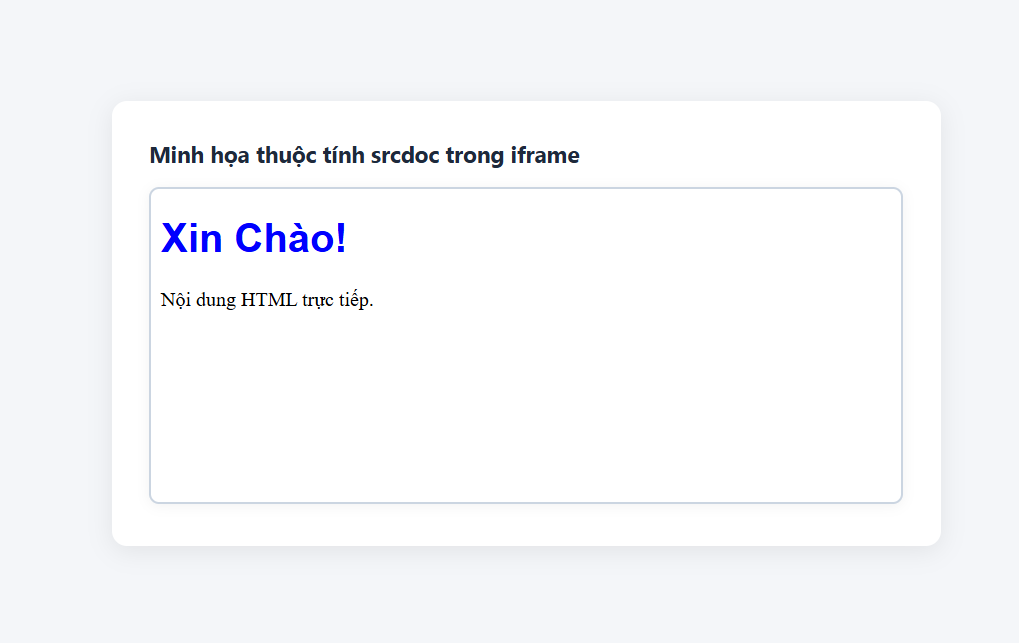
\includegraphics[width=0.7\linewidth]{figures/iframe_srcdoc_result.png}
\end{browserWindow}

% ------------------------------------------------------------------------------
\subsection{Bảng Tra Cứu Toàn Bộ Thuộc Tính Quan Trọng Của \taghint{<iframe>}}

\begin{prettyTableBox}[Bảng Tra Cứu Tất Cả Thuộc Tính Thẻ <iframe> Trong HTML5]
\rowcolors{2}{white}{primaryBlue!4}
\begin{tabularx}{\linewidth}{K{2.4cm} Z Z}
\rowcolor{primaryBlue}
\thd{Thuộc Tính} & \thd{Ý Nghĩa \& Chức Năng Cốt Lõi} & \thd{Ví dụ cú pháp Minh Họa} \\
\codeinline{src} & Đường dẫn URL trỏ tới tài liệu cần nhúng & \codeinline{<iframe src="https://example.com">} \\
\codeinline{srcdoc} & Nhúng trực tiếp chuỗi mã HTML (HTML5) & \codeinline{<iframe srcdoc="<h1>Hi</h1>">} \\
\codeinline{width} & Định nghĩa chiều rộng khung (pixel/percent) & \codeinline{<iframe width="600">} \\
\codeinline{height} & Định nghĩa chiều cao khung (pixel) & \codeinline{<iframe height="400">} \\
\codeinline{frameborder} & 0: Không viền, 1: Có viền (Khuyên dùng CSS) & \codeinline{<iframe frameborder="0">} \\
\codeinline{allowfullscreen} & Bật quyền mở chế độ xem toàn màn hình & \codeinline{<iframe allowfullscreen>} \\
\codeinline{sandbox} & Giới hạn quyền hạn và bảo mật nội dung & \codeinline{<iframe sandbox="allow-scripts">} \\
\codeinline{loading} & \codeinline{lazy} (tải khi cuộn), \codeinline{eager} (tải ngay) & \codeinline{<iframe loading="lazy">} \\
\codeinline{name} & Tên khung để liên kết với thuộc tính \codeinline{target} & \codeinline{<iframe name="myFrame">} \\
\end{tabularx}
\end{prettyTableBox}

% ------------------------------------------------------------------------------
\subsection{4 Trường Hợp Sử Dụng \taghint{<iframe>} Phổ Biến Trong Thực Tế Dự Án}

\paragraph{1. Nhúng một trang web mở (Ví dụ Wikipedia):}
\begin{codeWindow}[Mã Nguồn Nhúng Trang Web Wikipedia Vào Khung Iframe]
\begin{lstlisting}[language=HTML5]
<iframe src="https://www.wikipedia.org/" width="800" height="600"></iframe>
\end{lstlisting}
\end{codeWindow}

\begin{browserWindow}[https://www.wikipedia.org/]
\centering\vspace{2pt}
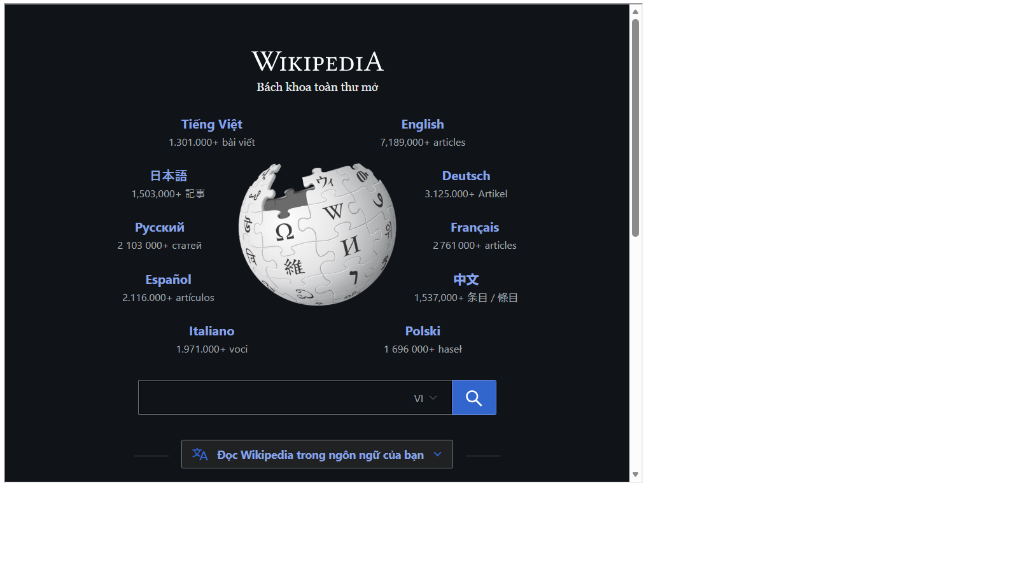
\includegraphics[width=0.7\linewidth]{figures/iframe_wikipedia_result.png}
\end{browserWindow}

\begin{noteBox}[Lưu Ý Quan Trọng Về Chính Sách X-Frame-Options]
Một số trang web lớn (như Google, Facebook) thiết lập Header bảo mật \codeinline{X-Frame-Options: DENY} hoặc \codeinline{SAMEORIGIN} nhằm ngăn chặn trang khác nhúng vào khung iframe để chống tấn công \term{Clickjacking}.
\end{noteBox}

\paragraph{2. Nhúng Video phát trực tuyến từ YouTube:}
YouTube cung cấp đường dẫn nhúng chuẩn qua định dạng \codeinline{/embed/VIDEO\_ID}:
\begin{codeWindow}[Mã Nguồn Nhúng Video YouTube Chuẩn Ngữ Nghĩa]
\begin{lstlisting}[language=HTML5]
<iframe width="560" height="315" 
        src="https://www.youtube.com/embed/dQw4w9WgXcQ" 
        allow="accelerometer; autoplay; clipboard-write; encrypted-media; gyroscope; picture-in-picture"
        allowfullscreen>
</iframe>
\end{lstlisting}
\end{codeWindow}

\begin{browserWindow}[https://www.youtube.com/embed/dQw4w9WgXcQ]
\centering\vspace{2pt}

\includegraphics[width=0.7\linewidth]{figures/iframe_youtube_thumbnail.png}
\end{browserWindow}

\paragraph{3. Nhúng Bản đồ tương tác Google Maps:}
\begin{codeWindow}[Mã Nguồn Nhúng Google Maps Vào Khung Web]
\begin{lstlisting}[language=HTML5]
<iframe width="600" height="450" 
        src="https://www.google.com/maps/embed?pb=!1m18!1m12!1m3!1d3151.835434509839!2d144.9630579153167!3d-37.81410797975171!2m3!1f0!2f0!3f0!3m2!1i1024!2i768!4f13.1!3m3!1m2!1s0x6ad642af0f11fd81%3A0xf5770f9af14bdf8d!2sFederation%20Square!5e0!3m2!1sen!2s!4v1589163966416!5m2!1sen!2s" 
        allowfullscreen>
</iframe>
\end{lstlisting}
\end{codeWindow}

\begin{browserWindow}[https://www.google.com/maps/embed]
\centering\vspace{2pt}
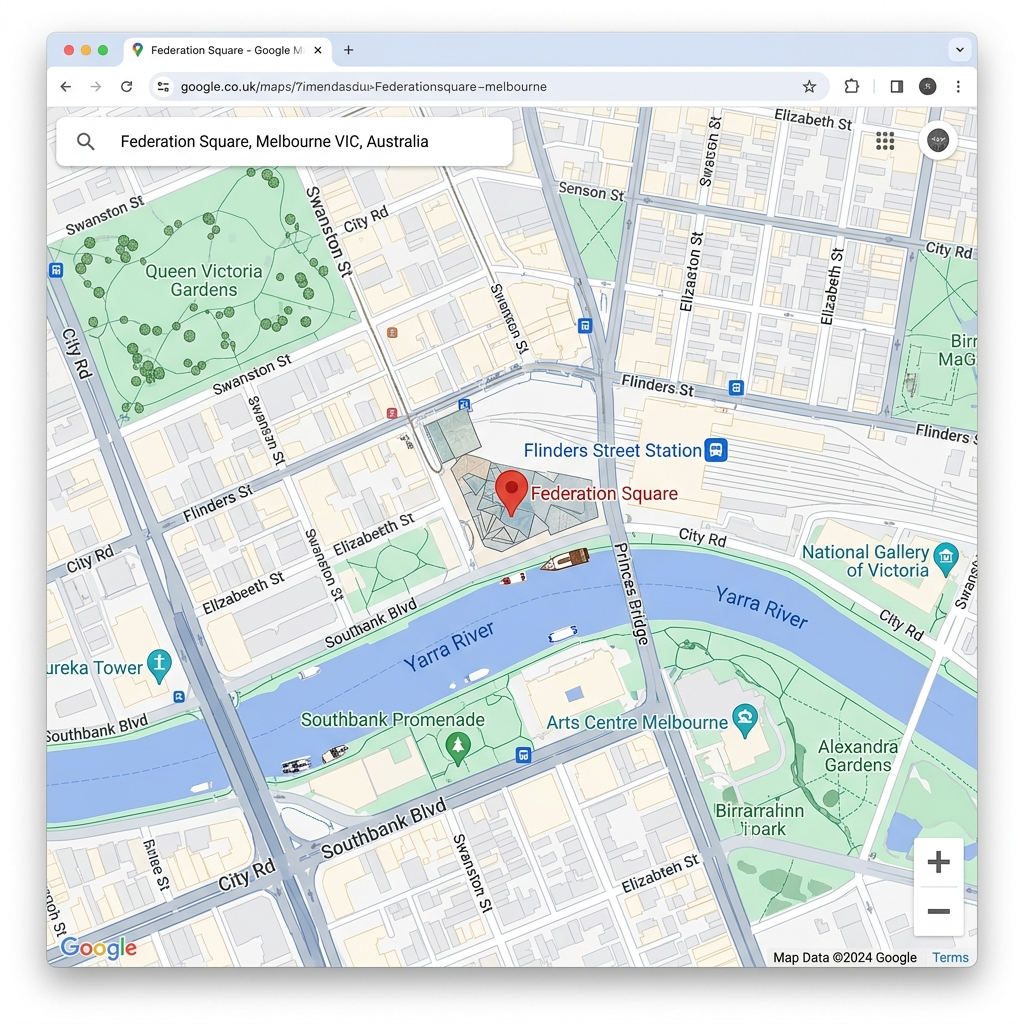
\includegraphics[width=0.7\linewidth]{figures/iframe_google_maps_thumbnail.png}
\end{browserWindow}

\paragraph{4. Nhúng Tài liệu báo cáo dạng tệp PDF:}
\begin{codeWindow}[Mã Nguồn Nhúng Trực Tiếp Tệp Tài Liệu PDF]
\begin{lstlisting}[language=HTML5]
<iframe src="document.pdf" width="800" height="600"></iframe>
\end{lstlisting}
\end{codeWindow}

\begin{browserWindow}[file:///project/document.pdf]
\centering\vspace{2pt}
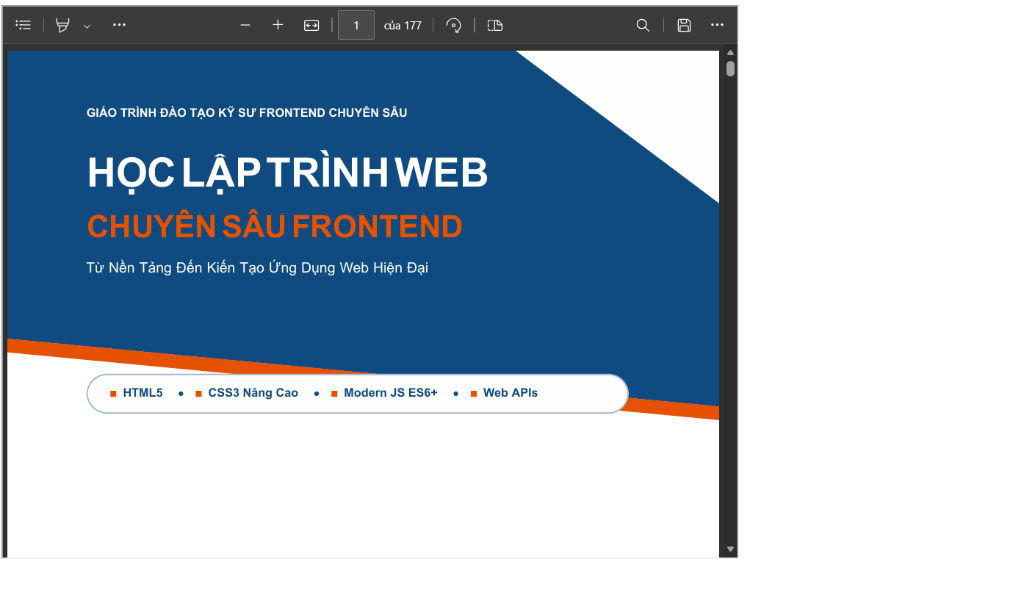
\includegraphics[width=0.7\linewidth]{figures/iframe_pdf_user_real.png}
\end{browserWindow}

% ------------------------------------------------------------------------------
\subsection{Hướng Dẫn Chi Tiết Quy Trình Lấy Đường Dẫn Nhúng (Embed Link)}

Một trong những sai lầm phổ biến nhất của lập trình viên mới bắt đầu là sao chép trực tiếp đường dẫn URL hiển thị trên thanh địa chỉ của trình duyệt để đưa vào thuộc tính \codeinline{src} của thẻ \codeinline{<iframe>}. Các nền tảng lớn như YouTube hay Google Maps đều sử dụng cơ chế bảo mật chống nhúng trực tiếp URL xem thông thường.

\begin{warnBox}[Cảnh Báo Bẫy Sai Lầm Thường Gặp Khi Lấy Link Nhúng]
\begin{itemize}[leftmargin=1.5em, itemsep=3pt, parsep=0pt]
    \item \textbf{SAI}: \codeinline{src="https://www.youtube.com/watch?v=VIDEO\_ID"} $\rightarrow$ Trình duyệt sẽ báo lỗi \term{Refused to display in a frame because it set 'X-Frame-Options' to 'sameorigin'}.
    \item \textbf{ĐÚNG}: \codeinline{src="https://www.youtube.com/embed/VIDEO\_ID"} $\rightarrow$ Sử dụng giao thức nhúng chuẩn do nền tảng cung cấp.
\end{itemize}
\end{warnBox}

\begin{tcolorbox}[enhanced, colback=codeBg, colframe=primaryBlue!30, arc=6pt, boxrule=0.8pt, top=10pt, bottom=10pt, left=12pt, right=12pt, title={\sffamily\bfseries\color{primaryBlue} Quy Trình 4 Bước Lấy Link Nhúng Video YouTube Chuẩn}, coltitle=primaryBlue, colbacktitle=primaryBlue!8, attach boxed title to top left={xshift=10pt, yshift=-10pt}, boxed title style={arc=4pt, boxrule=0.6pt, colframe=primaryBlue!40}]
\vspace{4pt}
\begin{description}[font=\sffamily\bfseries\color{primaryBlue}, leftmargin=4.8em, style=sameline, itemsep=6pt]
    \item[{\tcbox[colback=primaryBlue,coltext=white,boxsep=1pt,left=4pt,right=4pt,top=1pt,bottom=1pt,arc=3pt,fontupper=\sffamily\tiny\bfseries]{BƯỚC 1}}] Mở video cần nhúng trên trang web YouTube.
    \item[{\tcbox[colback=primaryBlue,coltext=white,boxsep=1pt,left=4pt,right=4pt,top=1pt,bottom=1pt,arc=3pt,fontupper=\sffamily\tiny\bfseries]{BƯỚC 2}}] Nhấp vào nút \textbf{Chia sẻ} (\textit{Share}) phía dưới khung phát video.
    \item[{\tcbox[colback=primaryBlue,coltext=white,boxsep=1pt,left=4pt,right=4pt,top=1pt,bottom=1pt,arc=3pt,fontupper=\sffamily\tiny\bfseries]{BƯỚC 3}}] Trong cửa sổ hiện ra, chọn biểu tượng \textbf{Nhúng} (\textit{Embed} - biểu tượng mã \codeinline{</>}).
    \item[{\tcbox[colback=primaryBlue,coltext=white,boxsep=1pt,left=4pt,right=4pt,top=1pt,bottom=1pt,arc=3pt,fontupper=\sffamily\tiny\bfseries]{BƯỚC 4}}] Nhấp nút \textbf{Sao chép} (\textit{Copy}) để lấy toàn bộ đoạn mã \codeinline{<iframe>} đã được tích hợp sẵn thuộc tính chuẩn.
\end{description}
\end{tcolorbox}

\begin{tipBox}[Mẹo Chuyển Đổi Nhanh URL YouTube Thành Embed Link]
Nếu chỉ có URL dạng xem thông thường: \codeinline{https://www.youtube.com/watch?v=dQw4w9WgXcQ}, bạn chỉ cần thay thế cụm \codeinline{watch?v=} bằng \codeinline{embed/} để tạo thành đường dẫn nhúng hợp lệ: \codeinline{https://www.youtube.com/embed/dQw4w9WgXcQ}.
\end{tipBox}

\begin{tcolorbox}[enhanced, colback=codeBg, colframe=secondaryTeal!40, arc=6pt, boxrule=0.8pt, top=10pt, bottom=10pt, left=12pt, right=12pt, title={\sffamily\bfseries\color{secondaryTeal} Quy Trình 4 Bước Lấy Link Nhúng Bản Đồ Google Maps}, coltitle=secondaryTeal, colbacktitle=secondaryTeal!8, attach boxed title to top left={xshift=10pt, yshift=-10pt}, boxed title style={arc=4pt, boxrule=0.6pt, colframe=secondaryTeal!40}]
\vspace{4pt}
\begin{description}[font=\sffamily\bfseries\color{secondaryTeal}, leftmargin=4.8em, style=sameline, itemsep=6pt]
    \item[{\tcbox[colback=secondaryTeal,coltext=white,boxsep=1pt,left=4pt,right=4pt,top=1pt,bottom=1pt,arc=3pt,fontupper=\sffamily\tiny\bfseries]{BƯỚC 1}}] Truy cập Google Maps (\codeinline{maps.google.com}) và tìm kiếm địa điểm/vị trí muốn hiển thị.
    \item[{\tcbox[colback=secondaryTeal,coltext=white,boxsep=1pt,left=4pt,right=4pt,top=1pt,bottom=1pt,arc=3pt,fontupper=\sffamily\tiny\bfseries]{BƯỚC 2}}] Tại bảng thông tin địa điểm ở góc trái, nhấp nút \textbf{Chia sẻ} (\textit{Share}).
    \item[{\tcbox[colback=secondaryTeal,coltext=white,boxsep=1pt,left=4pt,right=4pt,top=1pt,bottom=1pt,arc=3pt,fontupper=\sffamily\tiny\bfseries]{BƯỚC 3}}] Chuyển sang tab \textbf{Nhúng bản đồ} (\textit{Embed a map}).
    \item[{\tcbox[colback=secondaryTeal,coltext=white,boxsep=1pt,left=4pt,right=4pt,top=1pt,bottom=1pt,arc=3pt,fontupper=\sffamily\tiny\bfseries]{BƯỚC 4}}] Chọn kích thước mong muốn (Nhỏ, Vừa, Lớn) rồi nhấp nút \textbf{Sao chép thẻ HTML} (\textit{Copy HTML}).
\end{description}
\end{tcolorbox}

\paragraph{3. Cách nhúng tệp tài liệu PDF cục bộ hoặc trên máy chủ:}
Để nhúng tệp PDF vào trang web, chỉ cần đặt tệp PDF vào cùng thư mục dự án và khai báo đường dẫn tương đối trỏ trực tiếp tới tệp:
\begin{codeWindow}[Khai Báo Nguồn Tệp PDF Trong Cùng Thư Mục Dự Án]
\begin{lstlisting}[language=HTML5]
<!-- (*@Tệp document.pdf nằm cùng cấp thư mục với tệp index.html@*) -->
<iframe src="document.pdf" width="100%" height="600px"></iframe>

<!-- (*@Hoặc trỏ tới thư mục chứa tài liệu tĩnh@*) -->
<iframe src="./assets/pdf/bao-cao-2026.pdf" width="100%" height="600px"></iframe>
\end{lstlisting}
\end{codeWindow}

% ------------------------------------------------------------------------------

% ------------------------------------------------------------------------------
\subsection{Cơ Chế Bảo Mật Tấn Công Clickjacking \& Thuộc Tính sandbox}

\paragraph{Rủi ro bảo mật với Iframe:}
Nếu nhúng một trang web không rõ nguồn gốc, trang đó có thể chạy các kịch bản độc hại, đánh cắp Cookie hoặc đánh lừa người dùng nhấp vào các nút giả mạo (\term{Clickjacking Attack}).

\paragraph{Giải pháp thiết lập thuộc tính sandbox:}
Thuộc tính \codeinline{sandbox} tạo ra một môi trường cách ly (\term{Isolation Sandbox}) cực kỳ nghiêm ngặt. Khi khai báo \codeinline{sandbox}, mặc định trình duyệt sẽ vô hiệu hóa tất cả Script, Form submit, Popup và Same-origin access:
\begin{codeWindow}[Phân Quyền Chi Tiết Cho Iframe Bằng sandbox]
\begin{lstlisting}[language=HTML5]
<iframe src="https://example.com" 
        sandbox="allow-scripts allow-forms">
</iframe>
\end{lstlisting}
\end{codeWindow}

\begin{browserWindow}[https://example.com (sandbox="allow-scripts allow-forms")]
\centering\sffamily\vspace{4pt}
{\bfseries\color{accentOrange}\large Môi Trường Isolation Sandbox Active} \par\vspace{6pt}
\small\textbf{Quyền được cấp:} \codeinline{allow-scripts}, \codeinline{allow-forms} \par\vspace{4pt}
\small\textcolor{warnBorder}{\textbf{Bị khóa hoàn toàn:}} Bị cấm truy cập Cookie, LocalStorage và DOM của trang cha! \par\vspace{4pt}
\end{browserWindow}

% ------------------------------------------------------------------------------
\subsection{Kỹ Thuật Loại Bỏ Viền \& Định Kiểu CSS Hiện Đại}

Mặc định thẻ \codeinline{<iframe>} có đường viền 3D cổ điển. Trong thực tế dự án, lập trình viên sử dụng CSS để loại bỏ viền và làm mịn giao diện:

\begin{codeWindow}[Loại Bỏ Viền Iframe Bằng CSS3]
\begin{lstlisting}[language=HTML5]
<style>
  iframe {
      border: none;
      border-radius: 8px;
      box-shadow: 0 4px 12px rgba(0,0,0,0.1);
  }
</style>
\end{lstlisting}
\end{codeWindow}

\begin{browserWindow}[https://example.com (style="border: none; border-radius: 8px;")]
\centering\sffamily\vspace{4pt}
{\bfseries\color{tipBorder}\large Giao Diện Khung Iframe Đã Loại Bỏ Viền Bằng CSS} \par\vspace{6pt}
\small\color{darkText} Đường viền 3D thô cứng bị xóa hoàn toàn, thay bằng góc bo 8px và bóng mờ nhẹ sang trọng. \par\vspace{4pt}
\end{browserWindow}

% ------------------------------------------------------------------------------
\subsection{Bảng Đánh Giá Ưu Điểm \& Nhược Điểm Của \taghint{<iframe>}}

\begin{prettyTableBox}[Bảng Tổng Hợp Đánh Giá Ưu Điểm Và Nhược Điểm Của <iframe>]
\rowcolors{2}{white}{primaryBlue!4}
\begin{tabularx}{\linewidth}{Z Z}
\rowcolor{primaryBlue}
\thd{Ưu Điểm Nổi Bật} & \thd{Nhược Điểm \& Hạn Chế} \\
Nhúng dễ dàng nội dung độc lập từ website bên ngoài & Một số trang web chặn nhúng bằng Header \codeinline{X-Frame-Options} \\
Hỗ trợ trình chiếu Video YouTube, Bản đồ Maps, Tài liệu PDF & Làm tăng số lượng HTTP Requests, ảnh hưởng hiệu năng tải trang \\
Kiểm soát phân quyền bảo mật độc lập bằng \codeinline{sandbox} & Tiềm ẩn rủi ro tấn công Clickjacking nếu không kiểm soát \\
\end{tabularx}
\end{prettyTableBox}

% ------------------------------------------------------------------------------
\subsection{Chuyên Sâu Thuộc Tính name \& Kỹ Thuật Điều Hướng target}

\paragraph{1. Định nghĩa thuộc tính name trong <iframe>:}
Thuộc tính \codeinline{name} được sử dụng để đặt danh xưng cho khung iframe. Mục đích chính là làm điểm nhận kết quả (\term{Target Destination}) cho các thẻ liên kết \codeinline{<a target="...">} hoặc thẻ biểu mẫu \codeinline{<form target="...">}, giúp nạp nội dung mới vào trong iframe mà \textbf{KHÔNG CẦN TẢI LẠI TRANG CHÍNH}.

\paragraph{2. Ví dụ 1: Điều hướng nội dung tìm kiếm Cốc Cốc vào iframe Bing:}
\begin{codeWindow}[Mã Nguồn Liên Kết Thẻ <a> Với name Của <iframe>]
\begin{lstlisting}[language=HTML5]
<!-- (*@Khung Iframe hiển thị Bing mặc định, có tên@*) name="web_bing" -->
<iframe src="https://www.bing.com/" name="web_bing" width="1000" height="600"></iframe>

<!-- (*@Thẻ a trỏ target tới@*) name="web_bing" (*@của iframe@*) -->
<p>
  <a href="https://coccoc.com/search" target="web_bing">
    (*@Tìm kiếm trên Cốc Cốc@*)
  </a>
</p>
\end{lstlisting}
\end{codeWindow}

\begin{browserWindow}[https://www.bing.com (name="web\_bing")]
\centering\sffamily\vspace{4pt}
{\bfseries\color{primaryBlue}\large Khung Iframe nhận tín hiệu điều hướng: name="web\_bing"} \par\vspace{6pt}
\small Ban đầu hiển thị: \textcolor{primaryBlue}{\underline{https://www.bing.com/}} \par\vspace{4pt}
\small\textcolor{accentOrange}{$\rightarrow$ Khi nhấp liên kết bên dưới, nội dung tải Cốc Cốc trực tiếp vào khung này!} \par\vspace{8pt}
\textcolor{primaryBlue}{\underline{Tìm kiếm trên Cốc Cốc}} \quad \small\textcolor{codeComment}{(target="web\_bing")} \par\vspace{4pt}
\end{browserWindow}

\paragraph{Phân tích trình tự hoạt động chi tiết:}
\begin{description}[font=\sffamily\bfseries\color{primaryBlue}, leftmargin=4.8em, style=sameline, itemsep=4pt]
    \item[{\tcbox[colback=primaryBlue,coltext=white,boxsep=1pt,left=4pt,right=4pt,top=1pt,bottom=1pt,arc=3pt,fontupper=\sffamily\tiny\bfseries]{BƯỚC 1}}] Khi tải trang ban đầu, iframe nạp trang Bing (\codeinline{src="https://www.bing.com/"}).
    \item[{\tcbox[colback=primaryBlue,coltext=white,boxsep=1pt,left=4pt,right=4pt,top=1pt,bottom=1pt,arc=3pt,fontupper=\sffamily\tiny\bfseries]{BƯỚC 2}}] Người dùng nhấp vào đường link \textit{"Tìm kiếm trên Cốc Cốc"}.
    \item[{\tcbox[colback=primaryBlue,coltext=white,boxsep=1pt,left=4pt,right=4pt,top=1pt,bottom=1pt,arc=3pt,fontupper=\sffamily\tiny\bfseries]{BƯỚC 3}}] Do thẻ \codeinline{<a>} có thuộc tính \codeinline{target="web\_bing"}, trình duyệt tải trực tiếp nội dung Cốc Cốc vào khung iframe \codeinline{name="web\_bing"}.
\end{description}

\paragraph{Phân biệt thuộc tính target trong thẻ <a>:}
\begin{itemize}[leftmargin=1.8em, itemsep=3pt, parsep=0pt]
    \item \codeinline{target="\_blank"}: Mở liên kết trong một Tab / Cửa sổ mới.
    \item \codeinline{target="\_self"}: Mở liên kết ngay tại Tab hiện tại (Mặc định).
    \item \codeinline{target="tên\_iframe"}: Mở liên kết bên trong khung iframe có \codeinline{name="tên\_iframe"}.
\end{itemize}

\paragraph{3. Ví dụ 2: Điều hướng bài viết Wikipedia trong Iframe:}
\begin{codeWindow}[Mã Nguồn Liên Kết Bài Viết Wikipedia Vào Frame wiki\_frame]
\begin{lstlisting}[language=HTML5]
<iframe src="https://www.wikipedia.org/" name="wiki_frame" width="1000" height="600"></iframe>

<p>
  <a href="https://vi.wikipedia.org/wiki/Lap_trinh" target="wiki_frame">
    (*@Xem bài viết về Lập trình trên Wikipedia@*)
  </a>
</p>
\end{lstlisting}
\end{codeWindow}

\begin{browserWindow}[https://vi.wikipedia.org/wiki/Lap\_trinh (name="wiki\_frame")]
\centering\sffamily\vspace{4pt}
{\bfseries\color{primaryBlue}\large Nạp Bài Viết Lập Trình Vào Khung wiki\_frame} \par\vspace{6pt}
{\small\color{darkText} Nạp bài viết Lập trình trực tiếp vào khung mà không làm chuyển trang chính.} \par\vspace{4pt}
\textcolor{primaryBlue}{\underline{Xem bài viết về Lập trình trên Wikipedia}} \quad \small\textcolor{codeComment}{(target="wiki\_frame")} \par\vspace{4pt}
\end{browserWindow}

\paragraph{4. Ví dụ 3: Gửi dữ liệu Form kết quả vào khung Iframe:}
\begin{codeWindow}[Mã Nguồn Gửi Kết Quả Submit Form Trực Tiếp Vào Iframe]
\begin{lstlisting}[language=HTML5]
<iframe name="formResult" width="600" height="300"></iframe>

<form action="https://www.example.com/search" target="formResult">
    <input type="text" name="query" placeholder="(*@Nhập từ khóa...@*)">
    <button type="submit">(*@Tìm kiếm@*)</button>
</form>
\end{lstlisting}
\end{codeWindow}

\begin{browserWindow}[https://www.example.com/search?query=HTML5 (name="formResult")]
\centering\sffamily\vspace{4pt}
{\bfseries\color{secondaryTeal}\large Kết Quả Submit Form Hiển Thị Trong Khung formResult} \par\vspace{6pt}
{\small\color{darkText} Khi bấm Tìm kiếm, trang kết quả hiển thị trực tiếp ngay trong khung mà không làm nạp lại trang hiện tại.} \par\vspace{4pt}
\end{browserWindow}

% ------------------------------------------------------------------------------
\subsection{Phân Biệt Chi Tiết Thuộc Tính name Và id Trong \taghint{<iframe>}}

\begin{prettyTableBox}[Bảng So Sánh Chi Tiết Giữa Thuộc Tính name Và id Của <iframe>]
\rowcolors{2}{white}{primaryBlue!4}
\begin{tabularx}{\linewidth}{K{2.5cm} Z Z}
\rowcolor{primaryBlue}
\thd{Tiêu Chí So Sánh} & \thd{Thuộc Tính name} & \thd{Thuộc Tính id} \\
Mục đích chính & Định danh iframe để làm đích đến cho thuộc tính \codeinline{target} & Định danh duy nhất để thao tác với CSS hoặc JavaScript \\
Tính trùng lặp & Có thể lặp lại tên trên nhiều phần tử & \textbf{Tuyệt đối duy nhất} trên toàn trang \\
Tương tác \codeinline{target} & \textbf{Sử dụng trực tiếp} với \codeinline{<a target="...">} & Không thể dùng làm giá trị cho \codeinline{target} \\
Thao tác JavaScript & Ít phổ biến & \textbf{Rất phổ biến} (\codeinline{document.getElementById}) \\
\end{tabularx}
\end{prettyTableBox}

\begin{conceptBox}[Ma Trận Khi Nào Dùng name Và Khi Nào Dùng id Của Iframe]
\begin{itemize}[leftmargin=1.5em, itemsep=3pt, parsep=0pt]
    \item \textbf{Dùng name}: Khi muốn điều hướng liên kết \codeinline{<a target="name">} hoặc kết quả Form \codeinline{<form target="name">} vào bên trong iframe.
    \item \textbf{Dùng id}: Khi muốn áp dụng CSS (\codeinline{\#myFrame \{ border: none; \}}) hoặc lập trình JavaScript (\codeinline{document.getElementById("myFrame")}).
\end{itemize}
\end{conceptBox}

% ==============================================================================
% CHUYÊN ĐỀ CHUYÊN SÂU: THẺ SEMANTIC TRONG HTML5 (SEMANTIC HTML5 MASTERCLASS)
% ==============================================================================
\section{Chi Tiết Về Các Thẻ Semantic Trong HTML}
\label{sec:semantic_html5_masterclass}

\subsection{Thẻ Semantic Là Gì?}

\term{Thẻ Semantic (thẻ có ý nghĩa)} là các thẻ HTML mô tả ý nghĩa của nội dung bên trong nó thay vì chỉ đơn thuần là một khối (\codeinline{<div>}) hoặc một dòng (\codeinline{<span>}).

\begin{itemize}[leftmargin=1.8em, itemsep=4pt, parsep=0pt]
    \item \textbf{Bản chất kỹ thuật}: Cung cấp thông tin ngữ nghĩa rõ ràng cho cả máy tính (trình duyệt, công cụ tìm kiếm, trình đọc màn hình) và con người (lập trình viên).
    \item \textbf{Mục đích cốt lõi}: Giúp trình duyệt, công cụ tìm kiếm (SEO) và lập trình viên hiểu nội dung dễ dàng hơn.
\end{itemize}

\subsubsection{Ví Dụ So Sánh Trực Quan Giữa Thẻ Div Và Thẻ Semantic}

\begin{prettyTableBox}[So Sánh Cú Pháp: Non-Semantic (Div) vs. Semantic HTML5]
\rowcolors{2}{white}{primaryBlue!4}
\begin{tabularx}{\linewidth}{>{\sffamily\bfseries\color{primaryBlue}}C{3.0cm} Z Z}
\rowcolor{primaryBlue}
\thd{\sffamily Vùng Thành Phần} & \thd{\sffamily [Khó Bảo Trì] Cấu Trúc Div Soup} & \thd{\sffamily [Dễ Bảo Trì] Chuẩn Semantic HTML5} \\
Phần đầu trang & \codeinline{<div class="header">...</div>} & \codeinline{<header>...</header>} \\
Thanh điều hướng & \codeinline{<div class="nav">...</div>} & \codeinline{<nav>...</nav>} \\
Nội dung chính & \codeinline{<div class="content">...</div>} & \codeinline{<main>...</main>} \\
Chân trang & \codeinline{<div class="footer">...</div>} & \codeinline{<footer>...</footer>} \\
\end{tabularx}
\end{prettyTableBox}


\subsubsection{Sơ Đồ Minh Họa Bố Cục Trang Web: Div Soup vs Semantic Landmarks}

\begin{center}
\begin{tcolorbox}[
    enhanced,
    colback=codeBg!40!white,
    colframe=primaryBlue!30,
    arc=8pt,
    boxrule=0.8pt,
    drop shadow=black!4!white,
    top=14pt, bottom=14pt, left=10pt, right=10pt,
    title={\sffamily\bfseries\small\color{primaryBlue} SƠ ĐỒ SO SÁNH KIẾN TRÚC TRANG WEB: KHÔNG SEMANTIC VS SEMANTIC HTML5}
]
\centering
\begin{tikzpicture}[
    scale=0.85, transform shape,
    font=\sffamily\small,
    divNode/.style={fill=red!8, draw=red!50, rounded corners=3pt, inner sep=3pt, font=\fontsize{7pt}{9pt}\selectfont\ttfamily\bfseries\color{red!80!black}, align=center},
    semNode/.style={fill=primaryBlue!10, draw=primaryBlue!70, rounded corners=3pt, inner sep=3pt, font=\fontsize{7pt}{9pt}\selectfont\ttfamily\bfseries\color{primaryBlue}, align=center},
    arrowLine/.style={->, >=stealth, line width=1.5pt, color=accentOrange}
]

% Left Column: Non-semantic Div structure (x = 0 to 5.2cm, center at x = 2.6)
\node[divNode, minimum width=5.2cm] (dhead) at (2.6, 0) {<div class="header"> Header </div>};
\node[divNode, minimum width=5.2cm] (dnav) at (2.6, -0.75) {<div class="nav"> Navigation </div>};
\node[divNode, minimum width=3.3cm, minimum height=1.6cm] (dmain) at (1.65, -2.1) {<div class="content">\\Main Content\\</div>};
\node[divNode, minimum width=1.7cm, minimum height=1.6cm] (dside) at (4.35, -2.1) {<div class="side">\\Sidebar\\</div>};
\node[divNode, minimum width=5.2cm] (dfoot) at (2.6, -3.45) {<div class="footer"> Footer </div>};
\node[font=\sffamily\bfseries\small\color{red!80!black}] at (2.6, 0.65) {[Khó Bảo Trì] "Div Soup"};

% Middle Connecting Arrow (x = 5.2 to 7.8, arrow from 5.5 to 7.5)
\draw[arrowLine] (5.5, -2.1) -- (7.5, -2.1) 
    node[midway, above=3pt, font=\sffamily\bfseries\tiny\color{accentOrange}] {NÂNG CẤP}
    node[midway, below=3pt, font=\sffamily\tiny\color{darkText!70}] {Thẻ Ngữ Nghĩa};

% Right Column: Semantic HTML5 structure (x = 7.8 to 13.0cm, center at x = 10.4)
\node[semNode, minimum width=5.2cm] (shead) at (10.4, 0) {<header> Header </header>};
\node[semNode, minimum width=5.2cm] (snav) at (10.4, -0.75) {<nav> Navigation </nav>};
\node[semNode, minimum width=3.3cm, minimum height=1.6cm] (smain) at (9.45, -2.1) {<main>\\<article> Content </article>\\</main>};
\node[semNode, minimum width=1.7cm, minimum height=1.6cm] (sside) at (12.15, -2.1) {<aside>\\Sidebar\\</aside>};
\node[semNode, minimum width=5.2cm] (sfoot) at (10.4, -3.45) {<footer> Footer </footer>};
\node[font=\sffamily\bfseries\small\color{primaryBlue}] at (10.4, 0.65) {[Dễ Bảo Trì] Semantic HTML5};

\end{tikzpicture}
\end{tcolorbox}
\end{center}

% ==============================================================================
\subsection{Lợi Ích Của Thẻ Semantic}

Sử dụng thẻ Semantic mang lại 4 lợi ích lớn trong phát triển web chuyên nghiệp:

\begin{itemize}[leftmargin=1.8em, itemsep=6pt, parsep=0pt]
    \item \textbf{Tối ưu SEO}: Công cụ tìm kiếm dễ hiểu nội dung, giúp trang xếp hạng cao hơn trên kết quả tìm kiếm (Google, Bing).
    \item \textbf{Hỗ trợ truy cập (Accessibility - A11y)}: Người khiếm thị có thể sử dụng trình đọc màn hình (\textit{Screen Readers}) để điều hướng trang web dễ dàng hơn.
    \item \textbf{Dễ bảo trì \& nâng cấp}: Mã nguồn rõ ràng, dễ đọc, dễ hiểu cho lập trình viên khác khi tham gia vào dự án.
    \item \textbf{Giúp CSS dễ quản lý hơn}: Dùng đúng thẻ giúp giảm bớt class và ID không cần thiết trong tập tin CSS.
\end{itemize}

% ==============================================================================
\subsection{Danh Sách Các Thẻ Semantic Và Cách Sử Dụng}

Dưới đây là tổng hợp đầy đủ danh sách các thẻ Semantic phổ biến trong HTML5, chức năng kỹ thuật và ví dụ cú pháp đại diện:

\begin{prettyTableBox}[Danh Sách Các Thẻ Semantic HTML5 Và Ví Dụ Minh Họa]
\rowcolors{2}{white}{primaryBlue!4}
\begin{tabularx}{\linewidth}{>{\ttfamily\bfseries\color{primaryBlue}}K{2.2cm} Z Z}
\rowcolor{primaryBlue}
\thd{\sffamily Thẻ Semantic} & \thd{\sffamily Chức năng} & \thd{\sffamily Ví dụ minh họa cú pháp} \\

<header> & Phần đầu trang web (chứa logo, menu, tiêu đề). & \codeinline{<header><h1>Header</h1>}\newline\codeinline{</header>} \\

<nav> & Thanh điều hướng chứa menu liên kết. & \codeinline{<nav><a href="\#">Home</a></nav>} \\

<main> & Nội dung chính của trang web. & \codeinline{<main><h2>Nội dung</h2></main>} \\

<section> & Chia nội dung thành từng phần có chủ đề riêng. & \codeinline{<section><h2>Giới thiệu</h2></section>} \\

<article> & Bài viết độc lập như blog, tin tức. & \codeinline{<article><h2>Bài viết mới</h2></article>} \\

<aside> & Nội dung phụ như sidebar, quảng cáo. & \codeinline{<aside><h3>Tin liên quan</h3></aside>} \\

<footer> & Chân trang, chứa bản quyền, liên hệ. & \codeinline{<footer><p>\&copy; 2026</p></footer>} \\

<address> & Hiển thị thông tin liên hệ tác giả. & \codeinline{<address>info@example.com}\newline\codeinline{</address>} \\

<figure> & Nhóm hình ảnh hoặc biểu đồ minh họa. & \codeinline{<figure><img src="img.jpg"></figure>} \\

<figcaption> & Chú thích cho hình ảnh (dùng trong \codeinline{<figure>}). & \codeinline{<figcaption>Chú thích ảnh</figcaption>} \\

<mark> & Đánh dấu văn bản quan trọng (tô vàng). & \codeinline{<mark>Nội dung quan trọng</mark>} \\

<time> & Hiển thị ngày/giờ chuẩn máy đọc. & \codeinline{<time datetime="2026-07-26">}\newline\codeinline{  26/07/2026</time>} \\

<summary> & Tiêu đề cho nội dung thu gọn \codeinline{<details>}. & \codeinline{<summary>Xem chi tiết</summary>} \\

<details> & Hiển thị nội dung thu gọn/mở rộng khi click. & \codeinline{<details>}\newline\codeinline{  <summary>Mở</summary>}\newline\codeinline{</details>} \\

<dialog> & Hộp thoại pop-up trong HTML5. & \codeinline{<dialog open>Thông báo</dialog>} \\

<cite> & Trích dẫn nguồn tài liệu, bài báo. & \codeinline{<cite>HTML Mastery</cite>} \\

<code> & Hiển thị đoạn mã lập trình. & \codeinline{<code>console.log('Hi');</code>} \\
\end{tabularx}
\end{prettyTableBox}

% ==============================================================================
\subsection{Ví Dụ Sử Dụng Thực Tế Trong Một Trang Web}

Mã nguồn dưới đây minh họa cách kết hợp các thẻ Semantic để tạo dựng một cấu trúc trang web hoàn chỉnh tiêu chuẩn HTML5:

\begin{codeWindow}[Mã Nguồn Trang Web HTML5 Hoàn Chỉnh Sử Dụng Thẻ Semantic]
\begin{lstlisting}[language=HTML5]
<!DOCTYPE html>
<html lang="vi">
<head>
    <meta charset="UTF-8">
    <meta name="viewport" content="width=device-width, initial-scale=1.0">
    <title>(*@Website với Semantic HTML@*)</title>
</head>
<body>
    <header>
        <h1>(*@Website của tôi@*)</h1>
    </header>
    <nav>
        <a href="#">(*@Trang chủ@*)</a> | <a href="#">(*@Giới thiệu@*)</a> | <a href="#">(*@Liên hệ@*)</a>
    </nav>
    <main>
        <article>
            <h2>(*@Bài viết đầu tiên@*)</h2>
            <p>(*@Đây là nội dung bài viết.@*)</p>
        </article>
    </main>
    <aside>
        <h3>(*@Bài viết liên quan@*)</h3>
        <p>(*@Thêm nội dung hữu ích.@*)</p>
    </aside>
    <footer>
        <p>&copy; 2025 - (*@Bản quyền thuộc về tôi.@*)</p>
    </footer>
</body>
</html>
\end{lstlisting}
\end{codeWindow}

% ==============================================================================
\subsection{Tổng Kết: Vì Sao Nên Dùng Thẻ Semantic?}

\begin{prettyTableBox}[Tóm Tắt Lý Do Bắt Buộc Dùng Thẻ Semantic Trong Phát Triển Web]
\rowcolors{2}{white}{primaryBlue!4}
\begin{tabularx}{\linewidth}{>{\bfseries\color{primaryBlue}}C{4.5cm} Z}
\rowcolor{primaryBlue}
\thd{\sffamily Lợi ích} & \thd{\sffamily Lý do} \\
SEO tốt hơn & Công cụ tìm kiếm hiểu nội dung dễ dàng hơn. \\
Hỗ trợ người khuyết tật & Trình đọc màn hình đọc trang tốt hơn. \\
Dễ bảo trì code & Lập trình viên khác dễ hiểu cấu trúc trang web. \\
Dễ chỉnh sửa CSS & Nhắm đúng thẻ không cần nhiều class. \\
\end{tabularx}
\end{prettyTableBox}

\begin{conceptBox}[Tóm Lại]
Nên dùng thẻ Semantic thay vì \codeinline{<div>} nếu có thể, vì nó giúp trang web rõ ràng, dễ hiểu, thân thiện với SEO \& dễ bảo trì hơn!
\end{conceptBox}

% ==============================================================================
\subsection{Phân Tích Chi Tiết Danh Sách Một Số Thẻ Semantic Phổ Biến}

\subsubsection{1. Thẻ \codeinline{<header>} -- Phần Đầu Trang}
\textbf{Chức năng}: Chứa tiêu đề, logo, menu điều hướng, hoặc thông tin đầu trang.

\begin{codeWindow}[Mã Nguồn Mẫu Khai Báo Thẻ <header>]
\begin{lstlisting}[language=HTML5]
<header>
    <h1>(*@Chào mừng đến với Website@*)</h1>
    <nav>
        <ul>
            <li><a href="#">(*@Trang chủ@*)</a></li>
            <li><a href="#">(*@Giới thiệu@*)</a></li>
            <li><a href="#">(*@Liên hệ@*)</a></li>
        </ul>
    </nav>
</header>
\end{lstlisting}
\end{codeWindow}

\subsubsection{2. Thẻ \codeinline{<nav>} -- Thanh Điều Hướng}
\textbf{Chức năng}: Chứa danh sách liên kết để điều hướng trang web.

\begin{codeWindow}[Mã Nguồn Mẫu Khai Báo Thẻ <nav>]
\begin{lstlisting}[language=HTML5]
<nav>
    <ul>
        <li><a href="#">(*@Trang chủ@*)</a></li>
        <li><a href="#">(*@Sản phẩm@*)</a></li>
        <li><a href="#">(*@Liên hệ@*)</a></li>
    </ul>
</nav>
\end{lstlisting}
\end{codeWindow}

\begin{noteBox}[Lưu ý khi sử dụng thẻ <nav>]
Nên dùng \codeinline{<nav>} khi có nhóm liên kết chính, nếu chỉ có vài link nhỏ trong bài viết thì không cần.
\end{noteBox}

\subsubsection{3. Thẻ \codeinline{<section>} -- Phần Nội Dung}
\textbf{Chức năng}: Dùng để chia nội dung thành từng phần riêng biệt.

\begin{codeWindow}[Mã Nguồn Mẫu Khai Báo Thẻ <section>]
\begin{lstlisting}[language=HTML5]
<section>
    <h2>(*@Sản phẩm nổi bật@*)</h2>
    <p>(*@Danh sách các sản phẩm bán chạy nhất...@*)</p>
</section>
\end{lstlisting}
\end{codeWindow}

\begin{noteBox}[Lưu ý khi sử dụng thẻ <section>]
Dùng \codeinline{<section>} khi nội dung có chủ đề riêng và có tiêu đề (\codeinline{<h2>}, \codeinline{<h3>}...). Nếu không có tiêu đề, có thể dùng \codeinline{<div>} thay thế.
\end{noteBox}

\subsubsection{4. Thẻ \codeinline{<article>} -- Bài Viết Độc Lập}
\textbf{Chức năng}: Dùng cho nội dung tự tồn tại (bài báo, blog, tin tức).

\begin{codeWindow}[Mã Nguồn Mẫu Khai Báo Thẻ <article>]
\begin{lstlisting}[language=HTML5]
<article>
    <h2>(*@Học HTML5 cơ bản@*)</h2>
    <p>(*@HTML5 mang lại nhiều tính năng mới giúp lập trình viên...@*)</p>
</article>
\end{lstlisting}
\end{codeWindow}

\begin{conceptBox}[Phân biệt giữa <article> và <section>]
\begin{itemize}[leftmargin=1.5em, itemsep=2pt, parsep=0pt]
    \item \codeinline{<article>}: Nội dung có thể đọc độc lập (blog, tin tức).
    \item \codeinline{<section>}: Chỉ là phần trong trang web, thường có nhiều bài viết nhỏ.
\end{itemize}
\end{conceptBox}

\subsubsection{5. Thẻ \codeinline{<aside>} -- Nội Dung Bên Lề}
\textbf{Chức năng}: Dùng cho quảng cáo, danh sách liên quan, thanh bên (sidebar).

\begin{codeWindow}[Mã Nguồn Mẫu Khai Báo Thẻ <aside>]
\begin{lstlisting}[language=HTML5]
<aside>
    <h3>(*@Bài viết liên quan@*)</h3>
    <ul>
        <li><a href="#">(*@HTML cơ bản@*)</a></li>
        <li><a href="#">(*@CSS nâng cao@*)</a></li>
    </ul>
</aside>
\end{lstlisting}
\end{codeWindow}

\begin{noteBox}[Lưu ý khi sử dụng thẻ <aside>]
Nội dung không liên quan trực tiếp đến phần chính nhưng vẫn có ích.
\end{noteBox}

\subsubsection{6. Thẻ \codeinline{<footer>} -- Chân Trang}
\textbf{Chức năng}: Chứa thông tin bản quyền, liên hệ, link quan trọng.

\begin{codeWindow}[Mã Nguồn Mẫu Khai Báo Thẻ <footer>]
\begin{lstlisting}[language=HTML5]
<footer>
    <p>&copy; 2026 (*@Bản quyền thuộc về Website của tôi@*)</p>
    <p><a href="mailto:contact@example.com">(*@Liên hệ@*)</a></p>
</footer>
\end{lstlisting}
\end{codeWindow}

\begin{noteBox}[Lưu ý khi sử dụng thẻ <footer>]
Có thể có nhiều \codeinline{<footer>} trên trang, ví dụ trong mỗi \codeinline{<article>}.
\end{noteBox}

\subsubsection{7. Thẻ \codeinline{<figure>} Và \codeinline{<figcaption>} -- Ảnh Minh Họa}
\textbf{Chức năng}: Dùng để nhóm hình ảnh hoặc đồ họa với chú thích.


\begin{codeWindow}[Mã Nguồn Mẫu Khai Báo Thẻ <figure> và <figcaption>]
\begin{lstlisting}[language=HTML5]
<figure>
    <img src="image.jpg" alt="(*@Hình ảnh mô tả@*)">
    <figcaption>(*@Hình ảnh minh họa cho bài viết@*)</figcaption>
</figure>
\end{lstlisting}
\end{codeWindow}

\begin{noteBox}[Lưu ý khi sử dụng thẻ <figcaption>]
\codeinline{<figcaption>} là tùy chọn, giúp mô tả ảnh mà không cần thêm \codeinline{<p>}.
\end{noteBox}

% ==============================================================================
\subsection{Phân Tích Chuyên Sâu 4 Lý Do Vì Sao Nên Dùng Thẻ Semantic}

Thẻ Semantic giúp trang web có cấu trúc rõ ràng hơn so với việc chỉ sử dụng \codeinline{<div>}. Dưới đây là phân tích chi tiết 4 lý do chính:

\subsubsection{1. Giúp Trình Duyệt \& Công Cụ Tìm Kiếm (SEO) Hiểu Nội Dung Trang Web}
\begin{itemize}[leftmargin=1.8em, itemsep=3pt, parsep=0pt]
    \item Google, Bing, Cốc Cốc và các công cụ tìm kiếm khác có thể đọc hiểu trang web dễ dàng hơn nếu sử dụng các thẻ Semantic.
    \item Giúp xếp hạng SEO tốt hơn vì công cụ tìm kiếm có thể phân loại nội dung chính, nội dung phụ.
\end{itemize}

\begin{prettyTableBox}[So Sánh Giữa Khai Báo Không Rõ Ràng (Div) Và Khai Báo Semantic Rõ Ràng]
\rowcolors{2}{white}{primaryBlue!4}
\begin{tabularx}{\linewidth}{>{\sffamily\bfseries\color{primaryBlue}}C{3.0cm} Z Z}
\rowcolor{primaryBlue}
\thd{\sffamily Vùng Giao Diện} & \thd{\sffamily [Không Rõ Ràng] Dùng <div>} & \thd{\sffamily [Rõ Ràng] Dùng Thẻ Semantic} \\
Phần đầu trang & \codeinline{<div class="top">...</div>} & \codeinline{<header>...</header>} \\
Thanh menu & \codeinline{<div class="nav">...</div>} & \codeinline{<nav>...</nav>} \\
Nội dung chính & \codeinline{<div class="content">...</div>} & \codeinline{<main>...</main>} \\
Chân trang & \codeinline{<div class="bottom">...</div>} & \codeinline{<footer>...</footer>} \\
\end{tabularx}
\end{prettyTableBox}

\subsubsection{2. Cải Thiện Khả Năng Truy Cập (Accessibility - A11y) Cho Người Dùng Khuyết Tật}
\begin{itemize}[leftmargin=1.8em, itemsep=3pt, parsep=0pt]
    \item Trình đọc màn hình (\textit{screen readers}) có thể đọc hiểu nội dung dễ dàng hơn nếu dùng thẻ Semantic.
    \item Hỗ trợ người khiếm thị điều hướng trang web tốt hơn.
\end{itemize}

\begin{noteBox}[Minh Họa Tác Động Truy Cập (A11y)]
\begin{itemize}[leftmargin=1.5em, itemsep=2pt, parsep=0pt]
    \item Nếu có \codeinline{<nav>}, trình đọc màn hình biết đây là thanh menu thay vì chỉ là một \codeinline{<div>}.
    \item Nếu có \codeinline{<article>}, họ biết đây là nội dung chính thay vì phải đoán.
\end{itemize}
\end{noteBox}

\subsubsection{3. Dễ Bảo Trì \& Mở Rộng Code (Dễ Đọc Hiểu Hơn)}
\begin{itemize}[leftmargin=1.8em, itemsep=3pt, parsep=0pt]
    \item Nếu dùng thẻ Semantic, lập trình viên mới vào dự án dễ hiểu code hơn.
    \item Khi sửa hoặc cập nhật nội dung, dễ dàng tìm đúng vị trí cần chỉnh sửa.
\end{itemize}

\begin{prettyTableBox}[So Sánh Cấu Trúc Khó Bảo Trì Và Dễ Bảo Trì Trong Dự Án Web]
\rowcolors{2}{white}{primaryBlue!4}
\begin{tabularx}{\linewidth}{>{\sffamily\bfseries\color{primaryBlue}}C{3.0cm} Z Z}
\rowcolor{primaryBlue}
\thd{\sffamily Phần Tử Web} & \thd{\sffamily [Khó Bảo Trì] Dùng Div ID} & \thd{\sffamily [Dễ Bảo Trì] Dùng Thẻ Semantic} \\
Khối tiêu đề & \codeinline{<div id="header">...</div>} & \codeinline{<header>...</header>} \\
Khối menu & \codeinline{<div id="menu">...</div>} & \codeinline{<nav>...</nav>} \\
Khối nội dung & \codeinline{<div id="content">...</div>} & \codeinline{<main>...</main>} \\
Khối chân trang & \codeinline{<div id="footer">...</div>} & \codeinline{<footer>...</footer>} \\
\end{tabularx}
\end{prettyTableBox}
\begin{center}
$\rightarrow$ \textbf{Kết luận}: Dễ nhìn, dễ hiểu, dễ sửa đổi!
\end{center}

\subsubsection{4. Giúp CSS Dễ Quản Lý Hơn}
\begin{itemize}[leftmargin=1.8em, itemsep=3pt, parsep=0pt]
    \item CSS có thể target chính xác phần tử cần chỉnh sửa mà không cần đặt quá nhiều class hoặc ID.
\end{itemize}

\begin{prettyTableBox}[So Sánh Cách Chọn Phần Tử CSS Với Div Class Và Thẻ Semantic Direct Target]
\rowcolors{2}{white}{primaryBlue!4}
\begin{tabularx}{\linewidth}{>{\sffamily\bfseries\color{primaryBlue}}C{3.0cm} Z Z}
\rowcolor{primaryBlue}
\thd{\sffamily Quy Trình Viết CSS} & \thd{\sffamily [Phức Tạp] Dùng Class Cho Div} & \thd{\sffamily [Tối Ưu] Target Thẻ Semantic} \\
Khai báo CSS & \codeinline{.top { background: blue; }} & \codeinline{header { background: blue; }} \\
Cú pháp HTML & \codeinline{<div class="top">...</div>} & \codeinline{<header>...</header>} \\
\end{tabularx}
\end{prettyTableBox}

\begin{center}
$\rightarrow$ \textbf{Kết luận}: Giảm bớt code CSS dư thừa!
\end{center}

\begin{noteBox}[Tổng Kết Chung]
\begin{itemize}[leftmargin=1.5em, itemsep=3pt, parsep=0pt]
    \item \textbf{SEO tốt hơn}: Công cụ tìm kiếm hiểu nội dung dễ dàng hơn.
    \item \textbf{Hỗ trợ người khuyết tật}: Trình đọc màn hình đọc trang tốt hơn.
    \item \textbf{Dễ bảo trì code}: Lập trình viên khác dễ hiểu cấu trúc trang web.
    \item \textbf{Dễ chỉnh sửa CSS}: Nhắm đúng thẻ không cần nhiều class.
\end{itemize}
\textbf{Tóm lại}: Nên dùng thẻ Semantic thay vì \codeinline{<div>} nếu có thể, vì nó giúp trang web rõ ràng, dễ hiểu, thân thiện với SEO \& dễ bảo trì hơn!
\end{noteBox}

% ==============================================================================
% 13. MỤC "ĐỌC THÊM" (MỞ RỘNG KIẾN THỨC NÂNG CAO)
% ==============================================================================
\Needspace*{120pt}
\section{Đọc Thêm: Mở Rộng Kiến Thức Chuyên Sâu Về Semantic HTML5}
\label{sec:semantic_html5_advanced_readmore}

Phần đọc thêm cung cấp các góc nhìn chuyên sâu về nguyên lý hoạt động của trình duyệt, tương quan với chuẩn WAI-ARIA, thuật toán phân cấp cây tài liệu và các câu hỏi phỏng vấn tuyển dụng Frontend thực tế liên quan đến Semantic HTML.

\subsection{Sự Tương Quan Giữa Thẻ Semantic HTML5 Và WAI-ARIA Landmark Roles}

Trước khi HTML5 ra đời, W3C đã giới thiệu bộ tiêu chuẩn WAI-ARIA (\term{Web Accessibility Initiative - Accessible Rich Internet Applications}) để bổ sung thuộc tính \codeinline{role="..."} giúp trợ năng cho giao diện. Khi HTML5 chính thức được ban hành, các thẻ Semantic đã tự động tích hợp ngầm các ARIA Landmark Roles tương ứng:

\begin{prettyTableBox}[Ma Trận Tương Quan Giữa Thẻ Semantic HTML5 Và WAI-ARIA Landmark Roles]
\rowcolors{2}{white}{primaryBlue!4}
\begin{tabularx}{\linewidth}{>{\ttfamily\bfseries\color{primaryBlue}}K{2.5cm} >{\ttfamily\color{codeKeyword}}K{3.5cm} Z}
\rowcolor{primaryBlue}
\thd{\sffamily Thẻ Semantic HTML5} & \thd{\sffamily WAI-ARIA Role Tương Đương} & \thd{\sffamily Hành Vi Khả Năng Truy Cập (A11y Behavior)} \\

<header> & role="banner" & Xác định vùng tiêu đề hàng đầu của trang web hoặc bài viết. \\

<nav> & role="navigation" & Đánh dấu vùng điều hướng chính chứa danh sách liên kết. \\

<main> & role="main" & Đánh dấu trung tâm nội dung độc nhất của toàn trang. \\

<aside> & role="complementary" & Vùng bổ trợ thông tin, tách biệt khỏi luồng nội dung chính. \\

<footer> & role="contentinfo" & Chứa thông tin bản quyền, điều khoản dịch vụ và thông tin liên hệ. \\

<section> & role="region" & Vùng nội dung có chủ đề riêng (bắt buộc kết hợp thuộc tính aria-labelledby). \\

<form> & role="search" / role="form" & Đánh dấu vùng nhập liệu/tìm kiếm dữ liệu của người dùng. \\
\end{tabularx}
\end{prettyTableBox}

\begin{warnBox}[Cảnh Báo Kỹ Thuật: Tránh Khai Báo Thừa ARIA Roles]
Không nên khai báo trùng lặp như \codeinline{<nav role="navigation">} hay \codeinline{<main role="main">}. Đây là hành vi dư thừa mã (\textit{Redundant ARIA}) vì các trình duyệt hiện đại đã tự động gắn ngầm Landmark Role mặc định cho các thẻ Semantic HTML5 này.
\end{warnBox}

% ------------------------------------------------------------------------------
\subsection{Accessibility Tree (Cây Trợ Năng) Và Trình Đọc Màn Hình (Screen Readers)}

Khi trình duyệt tải tài liệu HTML, bên cạnh việc xây dựng cây \term{DOM (Document Object Model)}, trình duyệt còn song song tạo ra một cây phụ gọi là \term{Accessibility Tree (Cây Trợ Năng)}.

\begin{center}
\begin{tcolorbox}[
    enhanced, colback=codeBg!30!white, colframe=primaryBlue!25, arc=6pt, boxrule=0.8pt,
    top=10pt, bottom=10pt, left=12pt, right=12pt
]
\centering
\sffamily\small
\textbf{HTML Source Code} $\xrightarrow{\quad\text{Browser Parsing}\quad}$ \textbf{DOM Tree} (Render UI CSS) \\[4pt]
$\searrow\quad\text{Semantic Mapping}\quad$ \textbf{Accessibility Tree} (Screen Readers Voice API)
\end{tcolorbox}
\end{center}

Các phần mềm đọc màn hình phổ biến như \textbf{NVDA}, \textbf{JAWS} (trên Windows) hoặc \textbf{VoiceOver} (trên macOS/iOS) truy cập vào Cây Trợ Năng này để cung cấp phím tắt điều hướng nhanh cho người khiếm thị:
\begin{itemize}[leftmargin=1.8em, itemsep=3pt, parsep=0pt]
    \item Nhấn phím \codeinline{D} để nhảy nhanh qua các vùng Landmark (\codeinline{<header>}, \codeinline{<nav>}, \codeinline{<main>}, \codeinline{<footer>}).
    \item Nhấn phím \codeinline{H} để nhảy tuần tự qua các thẻ tiêu đề Heading (\codeinline{<h1>} đến \codeinline{<h6>}).
    \item Nhấn phím \codeinline{L} để nhảy đến danh sách liên kết (\codeinline{<nav>}).
\end{itemize}
Nếu trang web viết hoàn toàn bằng \codeinline{<div>}, Cây Trợ Năng sẽ hoàn toàn phẳng và người khuyết tật buộc phải đọc lướt từng từ một từ đầu đến cuối trang web.

% ------------------------------------------------------------------------------
\subsection{Thuật Toán Phân Mạch Nội Dung (HTML5 Outlining Algorithm)}

Trong đặc tả ban đầu của HTML5, W3C định nghĩa thuật toán \term{HTML5 Document Outlining Algorithm}. Theo đó, mỗi khi xuất hiện các phần tử bao bọc ngữ cảnh (\term{Sectioning Content}) như \codeinline{<article>}, \codeinline{<section>}, \codeinline{<aside>}, \codeinline{<nav>}, một phân cấp tiêu đề mới được thiết lập.

Tuy nhiên, các nhà phát triển trình duyệt (Chrome, Firefox, Safari) đã không triển khai đầy đủ thuật toán này. Vì vậy, \textbf{Best Practice hiện đại} được khuyến nghị bởi W3C và MDN là:
\begin{itemize}[leftmargin=1.8em, itemsep=3pt, parsep=0pt]
    \item Mỗi trang web chỉ nên có duy nhất một thẻ \codeinline{<h1>} dành cho tiêu đề chính đại diện trang.
    \item Tuân thủ chính xác thứ tự phân cấp tiêu đề giảm dần: \codeinline{<h1>} $\rightarrow$ \codeinline{<h2>} $\rightarrow$ \codeinline{<h3>} $\rightarrow$ \codeinline{<h4>}, tuyệt đối không nhảy cấp từ \codeinline{<h2>} xuống \codeinline{<h4>} chỉ vì lý do kích thước phông chữ CSS.
\end{itemize}

% ------------------------------------------------------------------------------
\subsection{Những Lỗi Phổ Biến Và Anti-Patterns Cần Tránh Khi Dùng Thẻ Semantic}

\begin{warnBox}[Top 4 Lỗi Sai Thường Gặp Của Lập Trình Viên Frontend Mới]
\begin{enumerate}[leftmargin=1.5em, itemsep=4pt, parsep=0pt]
    \item \textbf{Dùng thẻ <main> nhiều lần trên một trang}: Thẻ \codeinline{<main>} đại diện cho nội dung độc nhất của tài liệu. Chỉ được có duy nhất một thẻ \codeinline{<main>} hiển thị trên một trang web (trừ trường hợp các thẻ \codeinline{<main>} khác có thuộc tính \codeinline{hidden}).
    \item \textbf{Lạm dụng thẻ <section> để thay thế cho <div>}: \codeinline{<section>} dùng để nhóm nội dung có chung chủ đề và \textbf{phải có tiêu đề} (\codeinline{<h2>}-\codeinline{<h6>}). Nếu chỉ dùng để bọc khối nhằm mục đích căn chỉnh CSS layout hoặc style flexbox/grid, bắt buộc sử dụng thẻ \codeinline{<div>}.
    \item \textbf{Dùng thẻ <article> cho các khối giao diện nhỏ không độc lập}: Thẻ \codeinline{<article>} chỉ dùng khi nội dung đó có thể tách ra đứng độc lập và phân phối lại trên hệ thống khác (RSS Feed, mạng xã hội, tin tức).
    \item \textbf{Sử dụng sai thẻ <address>}: Thẻ \codeinline{<address>} chỉ dùng để cung cấp thông tin liên hệ của tác giả/chủ sở hữu bài viết hoặc website, không dùng để ghi địa chỉ bưu điện thông thường không liên quan đến tác giả.
\end{enumerate}
\end{warnBox}

% ------------------------------------------------------------------------------
\subsection{Góc Phỏng Vấn Frontend: Các Câu Hỏi Thường Gặp Về Semantic HTML}

\begin{conceptBox}[Bộ Câu Hỏi Phỏng Vấn Tuyển Dụng (Frontend Interview Q\&A)]
\begin{description}[font=\sffamily\bfseries\color{primaryBlue}, leftmargin=1.5em, itemsep=6pt]
    \item[Câu 1: Phân biệt sự khác nhau giữa <section> và <article>? Khi nào nên dùng thẻ nào?]
    \textit{Trả lời}: \codeinline{<article>} đại diện cho một khối nội dung độc lập, tự có nghĩa và có thể tái sử dụng độc lập ở nơi khác (ví dụ: bài viết blog, bình luận, thẻ sản phẩm). \codeinline{<section>} đại diện cho một phần nội dung gom nhóm theo chủ đề trong cùng một trang hoặc trong một article (ví dụ: phần giới thiệu, phần tính năng, phần liên hệ). Một \codeinline{<article>} có thể chứa nhiều \codeinline{<section>} và ngược lại một \codeinline{<section>} cũng có thể chứa nhiều \codeinline{<article>}.

    \item[Câu 2: Tại sao việc thay thế <div> bằng Semantic Tags lại cải thiện chỉ số SEO?]
    \textit{Trả lời}: Bot tìm kiếm của Google (Googlebot) sử dụng các thẻ Semantic để phân bổ trọng số từ khóa chính xác. Nội dung nằm trong \codeinline{<main>} và \codeinline{<article>} được đánh giá điểm ưu tiên cao nhất, trong khi nội dung trong \codeinline{<aside>} hay \codeinline{<footer>} được hạ trọng số. Việc sử dụng Semantic Tags giúp Bot hiểu chính xác cấu trúc cây dữ liệu mà không cần đoán dựa trên tên lớp CSS.

    \item[Câu 3: Thẻ <figure> và <figcaption> mang lại lợi ích gì hơn so với <img> đi kèm thẻ <p>?]
    \textit{Trả lời}: Thẻ \codeinline{<figure>} liên kết về mặt ngữ nghĩa giữa hình ảnh (hoặc sơ đồ, đoạn code) với phần văn bản chú thích \codeinline{<figcaption>}. Khi Trình đọc màn hình đọc đến phần tử này, nó sẽ thông báo cho người dùng biết đoạn văn bản chú thích đó thuộc về hình ảnh tương ứng, thay vì đọc rời rạc như hai phần tử độc lập.
\end{description}
\end{conceptBox}

\subsection{Nhóm Thẻ Semantic Mức Văn Bản (Text-Level / Inline Semantics)}

Bên cạnh nhóm thẻ Landmark quản lý bố cục khối, HTML5 cung cấp bộ thẻ ngữ nghĩa mức văn bản (\term{Text-level Semantics}) giúp đánh dấu chính xác ý nghĩa của từng từ, từng ký tự trong câu:

\begin{prettyTableBox}[Phân Tích Nhóm Thẻ Semantic Mức Văn Bản Chi Tiết]
\rowcolors{2}{white}{primaryBlue!4}
\begin{tabularx}{\linewidth}{>{\ttfamily\bfseries\color{primaryBlue}}K{2.2cm} Z Z}
\rowcolor{primaryBlue}
\thd{\sffamily Thẻ Semantic} & \thd{\sffamily Ý nghĩa ngữ nghĩa} & \thd{\sffamily Ví dụ cú pháp \& Chuẩn kỹ thuật} \\

<dfn> & Đánh dấu thuật ngữ lần đầu xuất hiện để định nghĩa. & \codeinline{Khái niệm <dfn>DOM</dfn> là...} \\

<abbr> & Từ viết tắt kèm giải thích đầy đủ qua \codeinline{title}. & \codeinline{<abbr title="HyperText}\newline\codeinline{  Markup Language">HTML</abbr>} \\

<kbd> & Tổ hợp phím nhập từ bàn phím người dùng. & \codeinline{Nhấn <kbd>Ctrl</kbd> + <kbd>S</kbd>} \\

<samp> & Kết quả đầu ra mẫu của chương trình/máy tính. & \codeinline{Hệ thống: <samp>500 Internal Error</samp>} \\

<var> & Tên biến số trong toán học hoặc mã lập trình. & \codeinline{Phương trình <var>y</var> = <var>f</var>(<var>x</var>)} \\

<data> & Gắn giá trị máy đọc được (\codeinline{value}) với chữ. & \codeinline{<data value="15000000">15 triệu</data>} \\

<time> & Thời gian máy đọc được (chuẩn ISO-8601). & \codeinline{<time datetime="2026-07-26">26/07/2026</time>} \\

<del> / <ins> & Văn bản bị xóa / Văn bản được chèn bổ sung. & \codeinline{<del>500k</del> <ins>400k</ins>} \\

<bdi> / <bdo> & Đảo chiều văn bản / Cách ly văn bản đa ngôn ngữ. & \codeinline{<bdo dir="rtl">Text</bdo>} \\
\end{tabularx}
\end{prettyTableBox}

\begin{codeWindow}[Mã Nguồn Mẫu Kết Hợp Các Thẻ Semantic Mức Văn Bản Nội Dòng]
\begin{lstlisting}[language=HTML5]
<p>
  Trong lap trinh Web, khai niem <dfn><abbr title="Document Object Model">DOM</abbr></dfn> la rat quan trong.
  Nguoi dung nhan to hop phim <kbd>Ctrl</kbd> + <kbd>Shift</kbd> + <kbd>I</kbd> de mo DevTools.
  Ket qua man hinh hien thi: <samp>200 OK</samp>.
  Thoi gian dang bai: <time datetime="2026-07-26T00:17:36+07:00">26/07/2026 00:17</time>.
  Khuyen mai tu <del datetime="2026-07-01">200.000d</del> (*@giảm xuống còn@*) <ins datetime="2026-07-26"><data value="150000">150.000(*@đ@*)</data></ins>.
</p>
\end{lstlisting}
\end{codeWindow}

% ------------------------------------------------------------------------------
\clearpage
\subsection{3 Mô Hình Kiến Trúc Bố Cụ Bằng Semantic Tags Trong Thực Tế}

\subsubsection{Mô Hình 1: Kiến Trúc Trang Bài Báo / Blog Công Nghệ (Article \& Comments)}

\begin{codeWindowBreakable}[Cấu Trúc Trang Bài Viết Công Nghệ Độc Lập Kèm Bình Luận Lồng Nhau]
\begin{lstlisting}[language=HTML5]
<main>
  <article>
    <header>
      <h1>Huong Dan Lam Chu Semantic HTML5 Tu A Den Z</h1>
      <p>Dang ngay: <time datetime="2026-07-26">26/07/2026</time></p>
      <address>Tac gia: <a href="mailto:admin@example.com">Nguyen Van A</a></address>
    </header>

    <section>
      <h2>1. Gioi thieu tong quan</h2>
      <p>Semantic HTML5 giup cau truc trang web mach lac...</p>
      <figure>
        <img src="semantic-diagram.png" alt="So do Semantic">
        <figcaption>Hinh 1: Kien truc Semantic HTML5 Landmarks</figcaption>
      </figure>
    </section>

    <footer>
      <p>Danh muc: <mark>Frontend Core</mark></p>
    </footer>

    <!-- Khu vuc binh luan (moi comment la mot article doc lap) -->
    <section>
      <h3>Binh luan tu doc gia</h3>
      <article>
        <header><b>Doc gia B</b> vao <time datetime="2026-07-26T09:00">09:00</time></header>
        <p>Bai viet rat chi tiet va de hieu!</p>
      </article>
    </section>
  </article>
</main>
\end{lstlisting}
\end{codeWindowBreakable}

\clearpage
\subsubsection{Mô Hình 2: Trang Chi Tiết Sản Phẩm Thương Mại Điện Tử (E-Commerce Product)}

\begin{codeWindowBreakable}[Cấu Trúc Trang Chi Tiết Sản Phẩm Thương Mại Điện Tử]
\begin{lstlisting}[language=HTML5]
<main>
  <article class="product-detail">
    <header>
      <h1>Laptop Macbook Pro M3 Max</h1>
      <p>Thuong hieu: <cite>Apple</cite></p>
    </header>

    <figure class="product-gallery">
      <img src="macbook-front.jpg" alt="Macbook Pro goc chinh dien">
      <figcaption>Hinh anh Macbook Pro M3 Max chinh hang</figcaption>
    </figure>

    <section class="pricing">
      <h2>Thong Tin Gia Ban</h2>
      <p>Gia goc: <del>55.000.000d</del></p>
      <p>Gia khuyen mai: <ins><data value="49990000">49.990.000d</data></ins></p>
      <p>Danh gia: <meter min="0" max="5" value="4.8">4.8 / 5 sao</meter></p>
    </section>

    <section class="specifications">
      <h2>Thong So Ky Thuat</h2>
      <ul>
        <li>Chipset: <var>Apple M3 Max</var></li>
        <li>RAM: <data value="36">36 GB Unified Memory</data></li>
      </ul>
    </section>
  </article>
</main>
\end{lstlisting}
\end{codeWindowBreakable}

\clearpage
\subsubsection{Mô Hình 3: Giao Diện Ứng Dụng Web / SaaS Dashboard Layout}

\begin{codeWindowBreakable}[Cấu Trúc Giao Diện Web Application / SaaS Dashboard]
\begin{lstlisting}[language=HTML5]
<!DOCTYPE html>
<html lang="vi">
<head><title>Admin SaaS Dashboard</title></head>
<body>
  <!-- Thanh App Header tren cung -->
  <header class="app-header">
    <h1>He Thong Quan Tri Enterprise</h1>
    <address>User Login: <a href="#">admin@company.com</a></address>
  </header>

  <div class="dashboard-wrapper">
    <!-- Thanh dieu huong Sidebar ben trai -->
    <nav class="app-sidebar">
      <ul>
        <li><a href="#analytics">Thong ke</a></li>
        <li><a href="#users">Nguoi dung</a></li>
        <li><a href="#settings">Cau hinh</a></li>
      </ul>
    </nav>

    <!-- Trung tam noi dung Dashboard -->
    <main class="app-content">
      <section id="analytics">
        <h2>Bao Cao Doanh Thu</h2>
        <p>Doanh thu thang nay: <data value="1200000000">1.2 Ty VND</data></p>
      </section>
    </main>

    <!-- Sidebar thong bao phu ben phai -->
    <aside class="notifications-panel">
      <h3>Thong Bao He Thong</h3>
      <p>Cap nhat phien ban <time datetime="2026-07-26">v2.4.0</time> thanh cong.</p>
    </aside>
  </div>

  <!-- Chan trang Status Bar -->
  <footer class="app-statusbar">
    <p>Trang thai he thong: <mark style="background-color: lightgreen;">ONLINE</mark></p>
  </footer>
</body>
</html>
\end{lstlisting}
\end{codeWindowBreakable}

% ------------------------------------------------------------------------------
\clearpage
\subsection{Tích Hợp Semantic HTML Với Dữ Liệu Có Cấu Trúc SEO (Schema.org \& Microdata)}

Để đạt điểm SEO tuyệt đối trên các công cụ tìm kiếm, trình duyệt không chỉ đọc thẻ Semantic mà còn giải mã bộ thuộc tính dữ liệu có cấu trúc (\term{Microdata Structured Data}) theo chuẩn \textbf{Schema.org}:

\begin{codeWindow}[Mã Nguồn Kết Hợp Thẻ Semantic Với Microdata Chuẩn Schema.org]
\begin{lstlisting}[language=HTML5]
<article itemscope itemtype="https://schema.org/TechArticle">
  <header>
    <h1 itemprop="headline">(*@Tổng Quan HTML5 Semantic Masterclass@*)</h1>
    <p>(*@Đăng bởi@*) <span itemprop="author" itemscope itemtype="https://schema.org/Person">
      <span itemprop="name">(*@Nguyễn Văn A@*)</span>
    </span></p>
    <time itemprop="datePublished" datetime="2026-07-26">26/07/2026</time>
  </header>

  <section itemprop="articleBody">
    <p>(*@Nội dung bài viết về Semantic HTML5...@*)</p>
  </section>
</article>
\end{lstlisting}
\end{codeWindow}

\begin{prettyTableBox}[Ma Trận Ánh Xạ Giữa Thẻ Semantic HTML5 Và Đối Tượng Dữ Liệu Schema.org]
\rowcolors{2}{white}{primaryBlue!4}
\begin{tabularx}{\linewidth}{>{\ttfamily\bfseries\color{primaryBlue}}K{2.8cm} >{\ttfamily\color{codeKeyword}}Z Z}
\rowcolor{primaryBlue}
\thd{\sffamily Thẻ Semantic HTML5} & \thd{\sffamily Schema.org Itemtype} & \thd{\sffamily Lợi Ích SEO Rich Snippets} \\

<article> & schema.org/Article & Hiển thị khung tin tức nổi bật trên Google SERP. \\

<figure> + <figcaption> & schema.org/ImageObject & Lập chỉ mục ảnh chuẩn trong Google Images Search. \\

<address> & schema.org/PostalAddress & Hiển thị Google Maps Local Business Knowledge Graph. \\

<main> & schema.org/MainContentPart & Giúp Googlebot xác định nội dung chính để xếp hạng SEO. \\
\end{tabularx}
\end{prettyTableBox}

% ------------------------------------------------------------------------------
\subsection{Hướng Dẫn Debug Cây Trợ Năng (Accessibility Panel Inspection)}

Để kiểm tra các thẻ Semantic HTML5 có hoạt động chuẩn xác trên trình duyệt Chrome hay không, kỹ sư Frontend thực hiện các bước sau:

\begin{center}
\begin{tcolorbox}[
    enhanced, colback=codeBg!40!white, colframe=primaryBlue!30, arc=8pt, boxrule=0.8pt,
    top=12pt, bottom=12pt, left=14pt, right=14pt,
    title={\sffamily\bfseries\small\color{primaryBlue} QUY TRÌNH 4 BƯỚC DEBUG ACCESSIBILITY TREE TRÊN CHROME DEVTOOLS}
]
\begin{enumerate}[leftmargin=1.5em, itemsep=4pt, parsep=0pt]
    \item \textbf{Bước 1}: Nhấp chuột phải vào phần tử trên trang web $\rightarrow$ chọn \codeinline{Inspect} (hoặc nhấn phím \codeinline{F12}).
    \item \textbf{Bước 2}: Chọn tab \codeinline{Elements} trên thanh công cụ Chrome DevTools.
    \item \textbf{Bước 3}: Tại khung bên phải, chọn tab phụ \codeinline{Accessibility}.
    \item \textbf{Bước 4}: Quan sát ô \textbf{Computed Properties} để xem các giá trị:
    \begin{itemize}[leftmargin=1.2em, itemsep=2pt, parsep=0pt]
        \item \codeinline{Role}: Vai trò ngữ nghĩa trình duyệt nhận diện (ví dụ: \codeinline{banner}, \codeinline{navigation}, \codeinline{main}).
        \item \codeinline{Name}: Tên phần tử đọc bởi Screen Reader (ví dụ: lấy từ thuộc tính \codeinline{aria-label} hoặc văn bản thẻ).
        \item \codeinline{Description}: Mô tả bổ sung chi tiết của phần tử.
    \end{itemize}
\end{enumerate}
\end{tcolorbox}
\end{center}
% ------------------------------------------------------------------------------
\Needspace*{120pt}
\subsection{Bộ Thẻ Semantic HTML5 Hiện Đại Mới Nhất (\taghint{<search>}, \taghint{<hgroup>}, \taghint{<meter>} vs \taghint{<progress>})}

Đặc tả WHATWG và W3C liên tục cập nhật bộ thẻ Semantic để đáp ứng sự phát triển của các ứng dụng web hiện đại. Dưới đây là phân tích kỹ thuật 3 nhóm thẻ ngữ nghĩa nâng cao quan trọng:

\subsubsection{1. Thẻ \codeinline{<search>} -- Chuẩn Ngữ Nghĩa Cho Khung Tìm Kiếm (HTML Specification 2023)}

Trước năm 2023, để đánh dấu khu vực tìm kiếm chuẩn A11y, lập trình viên phải gắn thuộc tính \codeinline{role="search"} thủ công vào thẻ \codeinline{<form>} hoặc \codeinline{<div>}. Thẻ \codeinline{<search>} chính thức ra đời nhằm cung cấp một Landmark Element native đại diện cho chức năng tìm kiếm:

\begin{codeWindow}[Mã Nguồn Mẫu Khai Báo Thẻ <search> Chuẩn Modern HTML]
\begin{lstlisting}[language=HTML5]
<!-- (*@Bao bọc khu vực tìm kiếm chính của website hoặc ứng dụng@*) -->
<search>
  <form action="/search" method="get">
    <label for="query">(*@Tìm kiếm bài viết:@*)</label>
    <input type="search" id="query" name="q" placeholder="(*@Nhập từ khóa...@*)">
    <button type="submit">(*@Tìm kiếm@*)</button>
  </form>
</search>
\end{lstlisting}
\end{codeWindow}

\begin{noteBox}[Lợi Ích Của Thẻ <search>]
Trình duyệt tự động gán Landmark Role \codeinline{search} vào Accessibility Tree, giúp Screen Readers nhảy nhanh tới ô tìm kiếm khi người dùng nhấn phím tắt điều hướng mà không cần khai báo thuộc tính ARIA bổ sung.
\end{noteBox}

\subsubsection{2. Thẻ \codeinline{<hgroup>} -- Nhóm Tiêu Đề Và Tagline/Subtitle}

Khi một bài viết hoặc phần tử có tiêu đề chính (\codeinline{<h1>}) đi kèm tiêu đề phụ, khẩu hiệu hoặc tagline, việc đặt thẻ tiêu đề thứ hai (\codeinline{<h2>}) trực tiếp bên dưới có thể làm sai lệch thuật toán phân cấp tiêu đề (Outlining Algorithm). Thẻ \codeinline{<hgroup>} giải quyết triệt để vấn đề này bằng cách gom nhóm chúng lại:

\begin{codeWindow}[Mã Nguồn Mẫu Sử Dụng Thẻ <hgroup>]
\begin{lstlisting}[language=HTML5]
<hgroup>
  <h1>(*@Giáo Trình HTML5 Masterclass@*)</h1>
  <p>(*@Hướng Dẫn Biên Soạn Chuyên Sâu Từ Cơ Bản Đến Nâng Cao Cho Frontend Developer@*)</p>
</hgroup>
\end{lstlisting}
\end{codeWindow}

\subsubsection{3. Ma Trận Phân Biệt Giữa Thẻ \taghint{<meter>} Và \taghint{<progress>}}

Hai thẻ \codeinline{<meter>} và \codeinline{<progress>} thường bị nhầm lẫn do giao diện mặc định có dạng thanh ngang trên trình duyệt. Tuy nhiên, về mặt ngữ nghĩa kỹ thuật, chúng phục vụ hai mục đích hoàn toàn riêng biệt:

\begin{prettyTableBox}[Ma Trận So Sánh Kỹ Thuật Giữa Thẻ <meter> Và <progress>]
\rowcolors{2}{white}{primaryBlue!4}
\begin{tabularx}{\linewidth}{>{\ttfamily\bfseries\color{primaryBlue}}K{2.0cm} Z Z}
\rowcolor{primaryBlue}
\thd{\sffamily Thẻ Semantic} & \thd{\sffamily Ngữ Nghĩa Kỹ Thuật} & \thd{\sffamily Ngữ Cảnh Sử Dụng Thực Tế} \\

<progress> & Biểu thị tiến độ hoàn thành của một tác vụ đang diễn ra (Dynamic Progress). & Tiến trình tải tập tin, tiến độ hoàn tất khóa học, thanh hoàn thành các bước thanh toán checkout. \\

<meter> & Đo lường một giá trị định lượng nằm trong một khoảng cố định (Scalar Gauge). & Dung lượng đĩa cứng đã dùng (80GB/100GB), mức dung lượng pin (45\%), điểm đánh giá chất lượng (4.5/5 sao). \\
\end{tabularx}
\end{prettyTableBox}

% ------------------------------------------------------------------------------
\Needspace*{120pt}
\subsection{Kỹ Thuật Responsive Image Semantics Với Thẻ \taghint{<picture>}}

Song song với thẻ \codeinline{<figure>} và \codeinline{<figcaption>}, thẻ \codeinline{<picture>} đại diện cho ngữ nghĩa trình diễn hình ảnh đáp ứng (\term{Responsive Image Semantics}). Thẻ này cho phép các kỹ sư Web thực hiện kỹ thuật \term{Art Direction} và tự động thương lượng định dạng ảnh tối ưu (\term{Format Negotiation}):

\begin{codeWindow}[Mã Nguồn Mẫu Sử Dụng Thẻ <picture> Tối Ưu Định Dạng Ảnh Và Viewport]
\begin{lstlisting}[language=HTML5]
<figure>
  <picture>
    <!-- (*@Ưu tiên định dạng AVIF thế hệ mới cho màn hình lớn Desktop@*) -->
    <source srcset="hero-large.avif" type="image/avif" media="(min-width: 1024px)">
    <!-- (*@Fallback định dạng WebP cho màn hình Tablet@*) -->
    <source srcset="hero-medium.webp" type="image/webp" media="(min-width: 768px)">
    <!-- (*@Fallback mặc định cho trình duyệt cũ hoặc màn hình Mobile@*) -->
    <img src="hero-small.jpg" alt="(*@Hình ảnh minh họa giao diện ứng dụng@*)">
  </picture>
  <figcaption>(*@Hình ảnh mô tả hệ thống responsive tương thích đa thiết bị@*)</figcaption>
</figure>
\end{lstlisting}
\end{codeWindow}

% ------------------------------------------------------------------------------
\Needspace*{120pt}
\subsection{Cấu Trúc Hộp Thoại Modal Native Với Thẻ \taghint{<dialog>}}

Thẻ \codeinline{<dialog>} cung cấp giải pháp native cho các hộp thoại pop-up, alert hoặc modal mà không cần xây dựng custom modal bằng \codeinline{<div>} phức tạp:

\begin{codeWindow}[Mã Nguồn Mẫu Khai Báo Thẻ <dialog> Native]
\begin{lstlisting}[language=HTML5]
<!-- (*@Thẻ dialog đóng vai trò modal popup@*) -->
<dialog id="confirmModal">
  <form method="dialog">
    <h2>(*@Xác Nhận Thao Tác@*)</h2>
    <p>(*@Bạn có chắc chắn muốn xóa dữ liệu này không?@*)</p>
    <button value="cancel">(*@Hủy bỏ@*)</button>
    <button value="confirm" value="default">(*@Xác nhận@*)</button>
  </form>
</dialog>
\end{lstlisting}
\end{codeWindow}

\begin{conceptBox}[Điểm Cốt Lõi Về Trợ Năng (A11y) Của Thẻ <dialog>]
Khi kích hoạt modal bằng phương thức JavaScript \codeinline{dialog.showModal()}:
\begin{itemize}[leftmargin=1.5em, itemsep=3pt, parsep=0pt]
    \item Trình duyệt tự động đưa hộp thoại vào \term{Top-Layer Stack} (hiển thị trên cùng toàn bộ giao diện mà không bị ảnh hưởng bởi z-index).
    \item Tự động tạo phần tử giả \codeinline{::backdrop} làm tối nền xung quanh.
    \item Kích hoạt cơ chế \term{Native Focus Trap}: Con trỏ bàn phím (phím \codeinline{Tab}) bị giữ chặt bên trong modal, không thể thoát ra các phần tử nền dưới.
    \item Cho phép người dùng nhấn phím \codeinline{ESC} để đóng modal nhanh chóng.
\end{itemize}
\end{conceptBox}

% ==============================================================================
% 12. TÓM TẮT CHƯƠNG 3
% ==============================================================================
\Needspace*{80pt}
\section{Tóm Tắt Chương 3}

\begin{noteBox}[Tổng Kết Cốt Lõi Chương 3]
HTML là ngôn ngữ nền tảng cốt lõi trong phát triển web. Việc làm chủ cấu trúc tài liệu HTML5, bộ thẻ ngữ nghĩa (Semantic HTML5 Masterclass), thực thể HTML, định dạng Bảng (Table) chuẩn mực và kết hợp đúng đắn với bộ thẻ \codeinline{<meta>} (tối ưu mã hóa UTF-8, Responsive Viewport, mô tả SEO và thẻ Open Graph mạng xã hội) sẽ giúp website vận hành chuẩn mực, đạt thứ hạng cao trên các công cụ tìm kiếm và mang lại trải nghiệm xuất sắc cho người dùng.
\end{noteBox}




% ==============================================================================
% CHƯƠNG 4: THẺ BỐ CỤC NGỮ NGHĨA & THẺ VĂN BẢN MASTERCLASS
% ==============================================================================
\chapter{Thẻ Bố Cục Ngữ Nghĩa (Layout Semantics) \& Thẻ Văn Bản}
\label{chap:semantic_structure}

Chương này trình bày chi tiết từng thẻ thuộc nhóm Bố cục ngữ nghĩa và nhóm Văn bản trong HTML5.

\section{Thẻ Thân Tài Liệu \taghint{<body>}}
\subsection{1. Lý Thuyết \& Thuộc Tính Sự Kiện Window}
Thẻ \codeinline{<body>} chứa toàn bộ nội dung trực quan hiển thị trên cửa sổ trình duyệt (Văn bản, Hình ảnh, Video, Biểu mẫu).

\begin{itemize}
    \item Các thuộc tính sự kiện cửa sổ: \codeinline{onload}, \codeinline{onunload}, \codeinline{onresize}, \codeinline{onpopstate}, \codeinline{ononline}, \codeinline{onoffline}.
\end{itemize}

\subsection{2. Ví Dụ Mã Nguồn Thực Tế}
\begin{codeWindow}[Mã Nguồn: Sử Dụng Thẻ body Với Sự Kiện Trạng Thái Mạng]
\begin{lstlisting}[language=HTML5]
<body ononline="(*@console.log('Đã kết nối Internet')@*)" onoffline="(*@alert('Mất kết nối mạng!')@*)">
  <h1>(*@Nội dung chính hiển thị tại đây@*)</h1>
</body>
\end{lstlisting}
\end{codeWindow}

\begin{browserWindow}[Kết Quả Hiển Thị Trình Duyệt: Thẻ <body>]
\sffamily
{\Huge\bfseries Nội dung chính hiển thị tại đây}
\end{browserWindow}

% ------------------------------------------------------------------------------
\section{Thẻ Đỉnh Trang / Đỉnh Phân Đoạn \taghint{<header>}}
\subsection{1. Lý Thuyết \& Quy Tắc Sử Dụng}
Thẻ \codeinline{<header>} đại diện cho nhóm các phần tử dẫn nhập hoặc điều hướng. Một trang web có thể chứa nhiều thẻ \codeinline{<header>} (một ở đỉnh trang web và các thẻ \codeinline{<header>} con nằm bên trong \codeinline{<article>} hoặc \codeinline{<section>}).

\subsection{2. Ví Dụ Mã Nguồn Thực Tế}
\begin{codeWindow}[Mã Nguồn: Thẻ Header Đỉnh Trang Web Chuẩn SEO]
\begin{lstlisting}[language=HTML5]
<header>
  <a href="/" class="logo">
    <img src="logo.svg" alt="EduWeb Academy">
  </a>
  <nav>
    <ul>
      <li><a href="/courses">(*@Khóa Học@*)</a></li>
      <li><a href="/blog">(*@Bài Viết@*)</a></li>
    </ul>
  </nav>
</header>
\end{lstlisting}
\end{codeWindow}

\begin{browserWindow}[Kết Quả Hiển Thị Trình Duyệt: Thẻ Header Đỉnh Trang]
\sffamily\small
\begin{tcolorbox}[colback=primaryBlue!5, colframe=primaryBlue!30, arc=5pt, boxsep=3pt, left=12pt, right=12pt, top=6pt, bottom=6pt]
\textcolor{primaryBlue}{\bfseries [LOGO] EduWeb Academy} \hfill \textcolor{primaryBlue}{\underline{Khóa Học}} \quad \textcolor{primaryBlue}{\underline{Bài Viết}}
\end{tcolorbox}
\end{browserWindow}

% ------------------------------------------------------------------------------
\section{Thẻ Thanh Điều Hướng \taghint{<nav>}}
\subsection{1. Lý Thuyết \& Accessibility (a11y)}
Thẻ \codeinline{<nav>} đại diện cho một phần của trang web chứa các liên kết điều hướng chính (Navigation Links). Trình đọc màn hình (Screen Reader) sử dụng thẻ này để giúp người khiếm thị nhảy nhanh đến menu chính.

\subsection{2. Ví Dụ Mã Nguồn Thực Tế}
\begin{codeWindow}[Mã Nguồn: Menu Điều Hướng Phân Tầng Với Thẻ Nav]
\begin{lstlisting}[language=HTML5]
<nav aria-label="(*@Thanh điều hướng chính@*)">
  <ul>
    <li><a href="/" aria-current="page">(*@Trang Chủ@*)</a></li>
    <li><a href="/about">(*@Giới Thiệu@*)</a></li>
    <li><a href="/contact">(*@Liên Hệ@*)</a></li>
  </ul>
</nav>
\end{lstlisting}
\end{codeWindow}

\begin{browserWindow}[Kết Quả Hiển Thị Trình Duyệt: Thanh Điều Hướng Nav]
\sffamily\small
\textcolor{primaryBlue}{\bfseries Trang Chủ} \quad$\bullet$\quad \textcolor{primaryBlue}{\underline{Giới Thiệu}} \quad$\bullet$\quad \textcolor{primaryBlue}{\underline{Liên Hệ}}
\end{browserWindow}

% ------------------------------------------------------------------------------
\section{Thẻ Nội Dung Chính \taghint{<main>}}
\subsection{1. Lý Thuyết \& Quy Tắc Độc Nhất}
Thẻ \codeinline{<main>} chứa nội dung độc nhất và trung tâm của tài liệu.

\begin{warnBox}[Quy Tắc Vàng Thẻ <main>]
Trong một tệp HTML chỉ được phép có \textbf{duy nhất 1 thẻ \codeinline{<main>} hiển thị}. Thẻ \codeinline{<main>} KHÔNG được là phần tử con của \codeinline{<header>}, \codeinline{<nav>}, \codeinline{<article>}, \codeinline{<aside>} hay \codeinline{<footer>}.
\end{warnBox}

\subsection{2. Ví Dụ Mã Nguồn Thực Tế}
\begin{codeWindow}[Mã Nguồn: Khối Nội Dung Chính Độc Nhất <main>]
\begin{lstlisting}[language=HTML5]
<main id="main-content">
  <h1>(*@Khóa Học HTML5 Masterclass@*)</h1>
  <p>(*@Nội dung chi tiết khóa học...@*)</p>
</main>
\end{lstlisting}
\end{codeWindow}

\begin{browserWindow}[Kết Quả Hiển Thị Trình Duyệt: Khối Nội Dung Chính Main]
\sffamily
{\Large\bfseries Khóa Học HTML5 Masterclass}\\[3pt]
{\small Nội dung chi tiết khóa học...}
\end{browserWindow}

% ------------------------------------------------------------------------------
\section{Thẻ Bài Viết Độc Lập \taghint{<article>}}
\subsection{1. Lý Thuyết \& Tiêu Chuẩn Tách Tải}
Thẻ \codeinline{<article>} đại diện cho một thành phần hoàn chỉnh, độc lập trong trang web mà có thể phân phối hoặc tái sử dụng độc lập (ví dụ: bài báo, sản phẩm thương mại điện tử, bài đăng blog, bình luận).

\subsection{2. Ví Dụ Mã Nguồn Thực Tế}
\begin{codeWindow}[Mã Nguồn: Thẻ Article Mô Phỏng UI Card Sản Phẩm Độc Lập]
\begin{lstlisting}[language=HTML5]
<article class="product-card">
  <img src="laptop.jpg" alt="Laptop Gaming">
  <h2>Laptop Gaming Pro 2026</h2>
  <p class="price">(*@25.000.000 VNĐ@*)</p>
  <button>(*@Thêm Vào Giỏ Hàng@*)</button>
</article>
\end{lstlisting}
\end{codeWindow}

\begin{browserWindow}[Kết Quả Hiển Thị Trình Duyệt: UI Card Sản Phẩm Article]
\sffamily\small
\begin{tcolorbox}[colback=white, colframe=gray!30, width=0.65\linewidth, arc=6pt, drop shadow=black!5!white]
\centering
\tcbox[on line, colback=gray!15, colframe=gray!30, arc=3pt]{\small\color{gray!80}[Hình ảnh Laptop Gaming]} \\[4pt]
{\bfseries Laptop Gaming Pro 2026}\\[2pt]
\textcolor{accentOrange}{\bfseries 25.000.000 VNĐ}\\[4pt]
\tcbox[on line, arc=3pt, colback=primaryBlue, colframe=primaryBlue, boxsep=2pt, left=8pt, right=8pt, top=2pt, bottom=2pt]{\color{white}\bfseries\small Thêm Vào Giỏ Hàng}
\end{tcolorbox}
\end{browserWindow}

% ------------------------------------------------------------------------------
\section{Thẻ Phân Đoạn Chủ Đề \taghint{<section>}}
\subsection{1. Lý Thuyết \& So Sánh \taghint{<section>} vs \taghint{<article>}}
Thẻ \codeinline{<section>} đại diện cho một phân đoạn độc lập chứa các nội dung cùng chung một chủ đề. Mỗi \codeinline{<section>} luôn luôn nên đi kèm với một thẻ tiêu đề (\codeinline{<h2>}-\codeinline{<h6>}).

\subsection{2. Ví Dụ Mã Nguồn Thực Tế}
\begin{codeWindow}[Mã Nguồn: Phân Đoạn Các Section Trong Bài Viết]
\begin{lstlisting}[language=HTML5]
<section id="introduction">
  <h2>(*@1. Giới Thiệu Căn Bản@*)</h2>
  <p>(*@Nội dung giới thiệu...@*)</p>
</section>

<section id="features">
  <h2>(*@2. Các Tính Năng Nổi Bật@*)</h2>
  <p>(*@Nội dung tính năng...@*)</p>
</section>
\end{lstlisting}
\end{codeWindow}

\begin{browserWindow}[Kết Quả Hiển Thị Trình Duyệt: Các Phân Đoạn Section]
\sffamily\small
{\bfseries\large 1. Giới Thiệu Căn Bản}\\[2pt]
Nội dung giới thiệu...\\[6pt]
{\bfseries\large 2. Các Tính Năng Nổi Bật}\\[2pt]
Nội dung tính năng...
\end{browserWindow}

\begin{prettyTableBox}[Bảng So Sánh Ngữ Nghĩa: <article> vs <section> vs <div>]
\small
\rowcolors{2}{white}{primaryBlue!4}
\begin{tabularx}{\linewidth}{K{2.2cm} Z Z K{3.5cm}}
\rowcolor{primaryBlue}
\thd{Thẻ HTML} & \thd{Ý Nghĩa Ngữ Nghĩa (Semantics)} & \thd{Đặc Điểm Độc Lập Nội Dung} & \thd{Trường Hợp Khuyên Dùng} \\
\codeinline{<article>} & Thành phần nội dung hoàn chỉnh, độc lập. & \textbf{Có thể phân phối độc lập} (Bản tin RSS, Widget, Card). & Bài viết blog, Tin tức, Sản phẩm eCommerce, Bình luận. \\
\codeinline{<section>} & Phân đoạn gom nhóm các ý thuộc cùng một chủ đề. & Cần đi kèm tiêu đề (\codeinline{<h2>}-\codeinline{<h6>}) để tạo Outline. & Các mục trong trang (Giới thiệu, Tính năng, Báo giá, FAQ). \\
\codeinline{<div>} & \textbf{Thẻ rỗng vô nghĩa} (Pure Container). & Không mang bất kỳ ý nghĩa ngữ nghĩa nào. & Phục vụ định kiểu CSS Flexbox/Grid hoặc JavaScript DOM. \\
\end{tabularx}
\end{prettyTableBox}

% ------------------------------------------------------------------------------
\section{Thẻ Thanh Bên Phụ \taghint{<aside>}}
\subsection{1. Lý Thuyết \& Mục Đích Sử Dụng}
Thẻ \codeinline{<aside>} chứa các nội dung liên quan gián tiếp đến nội dung chính xung quanh (như thanh bên Sidebar, bài viết liên quan, quảng cáo, ô trích dẫn).

\subsection{2. Ví Dụ Mã Nguồn Thực Tế}
\begin{codeWindow}[Mã Nguồn: Thanh Bên Phụ Aside Cho Trang Blog]
\begin{lstlisting}[language=HTML5]
<aside class="sidebar">
  <h3>(*@Bài Viết Được Xem Nhiều Nhất@*)</h3>
  <ul>
    <li><a href="/post/1">(*@Làm chủ CSS Grid@*)</a></li>
    <li><a href="/post/2">(*@Học JavaScript ES6@*)</a></li>
  </ul>
</aside>
\end{lstlisting}
\end{codeWindow}

\begin{browserWindow}[Kết Quả Hiển Thị Trình Duyệt: Thanh Bên Aside]
\sffamily\small
\begin{tcolorbox}[colback=secondaryTeal!5, colframe=secondaryTeal!30, width=0.75\linewidth, arc=5pt]
{\bfseries\color{secondaryTeal} Bài Viết Được Xem Nhiều Nhất}\\[4pt]
$\bullet$ \textcolor{primaryBlue}{\underline{Làm chủ CSS Grid}}\\[2pt]
$\bullet$ \textcolor{primaryBlue}{\underline{Học JavaScript ES6}}
\end{tcolorbox}
\end{browserWindow}

% ------------------------------------------------------------------------------
\section{Thẻ Chân Trang \taghint{<footer>}}
\subsection{1. Lý Thuyết \& Thành Phần Bên Trong}
Thẻ \codeinline{<footer>} đại diện cho chân của trang web hoặc chân của một phân đoạn \codeinline{<article>}. Thường chứa thông tin bản quyền, liên kết điều khoản dịch vụ, bản đồ trang web (Sitemap) và icon mạng xã hội.

\subsection{2. Ví Dụ Mã Nguồn Thực Tế}
\begin{codeWindow}[Mã Nguồn: Chân Trang Footer Đầy Đủ]
\begin{lstlisting}[language=HTML5]
<footer>
  <p>(*@\&copy; 2026 EduWeb Academy. Tất cả quyền được bảo lưu.@*)</p>
  <ul>
    <li><a href="/privacy">(*@Chính Sách Bảo Mật@*)</a></li>
    <li><a href="/terms">(*@Điều Khoản Sử Dụng@*)</a></li>
  </ul>
</footer>
\end{lstlisting}
\end{codeWindow}

\begin{browserWindow}[Kết Quả Hiển Thị Trình Duyệt: Chân Trang Footer]
\sffamily\small
\begin{tcolorbox}[colback=gray!10, colframe=gray!30, arc=4pt]
\centering
\small \copyright\; 2026 EduWeb Academy. Tất cả quyền được bảo lưu.\\[3pt]
\textcolor{primaryBlue}{\underline{Chính Sách Bảo Mật}} \quad$\vert$\quad \textcolor{primaryBlue}{\underline{Điều Khoản Sử Dụng}}
\end{tcolorbox}
\end{browserWindow}

% ------------------------------------------------------------------------------
\section{Thẻ Thông Tin Liên Hệ \taghint{<address>}}
\subsection{1. Lý Thuyết \& Định Dạng Chuẩn}
Thẻ \codeinline{<address>} cung cấp thông tin liên hệ cho tác giả hoặc chủ sở hữu của tài liệu/bài viết.

\subsection{2. Ví Dụ Mã Nguồn Thực Tế}
\begin{codeWindow}[Mã Nguồn: Thông Tin Liên Hệ Tác Giả Với Thẻ Address]
\begin{lstlisting}[language=HTML5]
<address>
  (*@Viết bởi@*) <a href="mailto:tan@eduweb.vn">(*@Nguyễn Trọng Tấn@*)</a>.<br>
  (*@Địa chỉ: Tòa nhà EduWeb, Hà Nội, Việt Nam.<br>@*)
  (*@Điện thoại: <a href="tel:+84987654321">0987 654 321</a>@*)
</address>
\end{lstlisting}
\end{codeWindow}

\begin{browserWindow}[Kết Quả Hiển Thị Trình Duyệt: Thẻ Address]
\sffamily\small
\textit{Viết bởi} \textcolor{primaryBlue}{\underline{Nguyễn Trọng Tấn}}.<br>
\textit{Địa chỉ: Tòa nhà EduWeb, Hà Nội, Việt Nam.}<br>
\textit{Điện thoại:} \textcolor{primaryBlue}{\underline{0987 654 321}}
\end{browserWindow}

% ------------------------------------------------------------------------------
\section{Nhóm Thẻ Tiêu Đề \taghint{<h1>} đến \taghint{<h6>} \& \taghint{<hgroup>}}
\subsection{1. Lý Thuyết \& Cây Phân Tầng Tiêu Đề SEO}
Các thẻ từ \codeinline{<h1>} đến \codeinline{<h6>} đại diện cho 6 cấp độ tiêu đề phân tầng. Thẻ \codeinline{<hgroup>} dùng để nhóm một tiêu đề chính và các tiêu đề phụ lại với nhau.

\subsection{2. Ví Dụ Mã Nguồn Thực Tế}
\begin{codeWindow}[Mã Nguồn: Cấu Trúc Hgroup Và Tiêu Đề Phân Tầng]
\begin{lstlisting}[language=HTML5]
<hgroup>
  <h1>(*@Lập Trình Web Chuyên Sâu@*)</h1>
  <p>(*@Giáo trình Bách khoa toàn thư Frontend 2026@*)</p>
</hgroup>
\end{lstlisting}
\end{codeWindow}

\begin{browserWindow}[Kết Quả Hiển Thị Trình Duyệt: Hgroup \& Tiêu Đề Phân Tầng]
\sffamily
{\Huge\bfseries Lập Trình Web Chuyên Sâu}\\[2pt]
{\color{gray!80}\Large Giáo trình Bách khoa toàn thư Frontend 2026}
\end{browserWindow}

% ------------------------------------------------------------------------------
\section{Thẻ Khối Chứa Tìm Kiếm \taghint{<search>}}
\subsection{1. Lý Thuyết \& Chuẩn WHATWG Mới}
Thẻ \codeinline{<search>} là thẻ ngữ nghĩa mới được đưa vào HTML Living Standard đại diện cho khối giao diện chứa công cụ tìm kiếm và lọc dữ liệu.

\subsection{2. Ví Dụ Mã Nguồn Thực Tế}
\begin{codeWindow}[Mã Nguồn: Thẻ Search Chứa Form Tìm Kiếm Chuẩn WHATWG]
\begin{lstlisting}[language=HTML5]
<search>
  <form action="/search" method="GET">
    <label for="query">(*@Tìm khóa học:@*)</label>
    <input type="search" id="query" name="q" placeholder="(*@Nhập từ khóa...@*)">
    <button type="submit">(*@Tìm Kiếm@*)</button>
  </form>
</search>
\end{lstlisting}
\end{codeWindow}

\begin{browserWindow}[Kết Quả Hiển Thị Trình Duyệt: Khối Tìm Kiếm Search]
\sffamily\small
\textbf{Tìm khóa học:} \;\;
\tcbox[on line, arc=3pt, colback=white, colframe=gray!40, left=6pt, right=30pt, top=3pt, bottom=3pt]{\color{gray!70}Nhập từ khóa...} \;\;
\tcbox[on line, arc=3pt, colback=primaryBlue, colframe=primaryBlue, left=8pt, right=8pt, top=3pt, bottom=3pt]{\color{white}\bfseries Tìm Kiếm}
\end{browserWindow}

\subsection{3. Đọc Thêm: Hệ Thống ARIA Landmarks \& Accessibility Tree}

Khi trình duyệt phân tích các thẻ Bố cục ngữ nghĩa HTML5, nó tự động ánh xạ (\textit{mapping}) các thẻ này thành các \term{Vùng Mốc ARIA (Landmark Roles)} trên Cây Trợ Năng (\term{Accessibility Tree}) mà không cần viết thủ công thuộc tính \codeinline{role="..."}:

\begin{prettyTableBox}[Bảng Ánh Xạ Thẻ Bố Cục HTML5 Sang ARIA Landmarks]
\small
\rowcolors{2}{white}{primaryBlue!4}
\begin{tabularx}{\linewidth}{K{2.8cm} K{3.5cm} Z}
\rowcolor{primaryBlue}
\thd{Thẻ Bố Cục HTML5} & \thd{ARIA Role Tương Đương} & \thd{Hành Vi Trình Đọc Màn Hình (Screen Reader)} \\
\codeinline{<header>} & \codeinline{role="banner"} & Giúp người khiếm thị định vị vùng đầu trang chứa Logo và Tiêu đề. \\
\codeinline{<nav>} & \codeinline{role="navigation"} & Cho phép ấn phím tắt nhảy trực tiếp đến danh sách liên kết điều hướng. \\
\codeinline{<main>} & \codeinline{role="main"} & Bỏ qua toàn bộ Menu để đi thẳng vào nội dung chính của trang web. \\
\codeinline{<aside>} & \codeinline{role="complementary"} & Đánh dấu khu vực thông tin phụ hỗ trợ cho nội dung chính. \\
\codeinline{<footer>} & \codeinline{role="contentinfo"} & Định vị vùng thông tin bản quyền và liên kết chân trang. \\
\codeinline{<search>} & \codeinline{role="search"} & Đánh dấu vùng công cụ tìm kiếm dữ liệu. \\
\end{tabularx}
\end{prettyTableBox}

% ------------------------------------------------------------------------------
\section{Thẻ Đoạn Văn \taghint{<p>} \& Khối Văn Bản Giữ Nguyên \taghint{<pre>}}
\subsection{1. Lý Thuyết \& Khác Biệt Cốt Lõi}
- \codeinline{<p>}: Đoạn văn bản thông thường (Trình duyệt tự động nén nhiều khoảng trắng liền nhau thành 1 khoảng trắng).
- \codeinline{<pre>}: Định dạng văn bản giữ nguyên chính xác từng khoảng trắng, dấu cách và xuống dòng như trong mã nguồn.

\subsection{2. Ví Dụ Mã Nguồn Thực Tế}
\begin{codeWindow}[Mã Nguồn: So Sánh Thẻ p và Thẻ pre]
\begin{lstlisting}[language=HTML5]
<!-- (*@Đoạn văn bình thường@*) --><p>(*@Đây là một đoạn văn bản chuẩn.@*)</p>

<!-- (*@Khối hiển thị giữ nguyên khoảng trắng@*) --><pre>
  (*@Họ và Tên    : Nguyễn Văn A@*)
  (*@Quê Quán     : Hà Nội@*)
</pre>
\end{lstlisting}
\end{codeWindow}

\begin{browserWindow}[Kết Quả Hiển Thị Trình Duyệt: So Sánh Thẻ p vs Thẻ pre]
\sffamily\small
\textbf{Thẻ <p> (Dòng chảy chuẩn):}\\[2pt]
Đây là một đoạn văn bản chuẩn.\\[6pt]
\textbf{Thẻ <pre> (Giữ nguyên khoảng trắng font Monospace):}\\[2pt]
\begin{tcolorbox}[colback=gray!8, colframe=gray!20, boxrule=0.5pt, arc=3pt]
\ttfamily\small
Họ và Tên    : Nguyễn Văn A\\
Quê Quán     : Hà Nội
\end{tcolorbox}
\end{browserWindow}

\begin{conceptBox}[Cơ Chế Nén Khoảng Trắng (Whitespace Collapse)]
\begin{itemize}[leftmargin=1.5em, itemsep=3pt]
    \item \textbf{Thẻ \codeinline{<p>}}: Áp dụng quy tắc nén khoảng trắng (\term{Whitespace Collapse}). Mọi dấu cách thừa, dấu Tab và ký tự xuống dòng trong mã nguồn đều bị trình duyệt nén lại thành \textbf{duy nhất 1 dấu cách}.
    \item \textbf{Thẻ \codeinline{<pre>}}: Vô hiệu hóa quy tắc nén khoảng trắng. Trình duyệt hiển thị chính xác từng ký tự khoảng trắng và dòng mới với phông chữ độ rộng cố định (\term{Monospace Font}).
    \item \textbf{Mẹo CSS Thay Thế}: Thay vì dùng thẻ \codeinline{<pre>}, bạn có thể dùng thẻ \codeinline{<p>} đính kèm CSS \codeinline{white-space: pre-wrap;} để vừa giữ nguyên khoảng trắng vừa hỗ trợ tự động xuống dòng khi màn hình nhỏ.
\end{itemize}
\end{conceptBox}

% ------------------------------------------------------------------------------
\section{Thẻ Trích Dẫn Khối \taghint{<blockquote>} \& Trích Dẫn Nội Dòng \taghint{<q>}}
\subsection{1. Lý Thuyết \& Thuộc Tính cite}
- \codeinline{<blockquote>}: Trích dẫn một đoạn văn bản dài từ nguồn khác (Hiển thị lùi lề khối).
- \codeinline{<q>}: Trích dẫn ngắn nằm trực tiếp trong dòng (Trình duyệt tự động thêm dấu ngoặc kép \codeinline{"..."}).
- Thuộc tính \codeinline{cite="..."}: Chứa URL nguồn gốc của bài trích dẫn.

\subsection{2. Ví Dụ Mã Nguồn Thực Tế}
\begin{codeWindow}[Mã Nguồn: Thẻ Blockquote và Thẻ q Với Thuộc Tính Cite]
\begin{lstlisting}[language=HTML5]
<blockquote cite="https://w3.org/TR/html5">
  <p>(*@HTML5 là chuẩn Living Standard phát triển bởi WHATWG.@*)</p>
</blockquote>

<p>(*@Tim Berners-Lee từng nói:@*) <q cite="https://quote.com">(*@Internet là dành cho tất cả mọi người@*)</q>.</p>
\end{lstlisting}
\end{codeWindow}

\begin{browserWindow}[Kết Quả Hiển Thị Trình Duyệt: Blockquote \& Quoted Text]
\sffamily\small
\begin{tcolorbox}[colback=primaryBlue!4, colframe=primaryBlue!40, leftrule=3pt, boxrule=0pt, arc=0pt]
\textit{HTML5 là chuẩn Living Standard phát triển bởi WHATWG.}
\end{tcolorbox}
Tim Berners-Lee từng nói: "Internet là dành cho tất cả mọi người".
\end{browserWindow}

% ------------------------------------------------------------------------------
\section{Các Thẻ Danh Sách \taghint{<ol>}, \taghint{<ul>}, \taghint{<li>}, \taghint{<dl>}, \taghint{<dt>}, \taghint{<dd>}}
\subsection{1. Lý Thuyết \& Các Thuộc Tính Danh Sách}
- \codeinline{<ul>}: Danh sách không thứ tự (Dấu chấm tròn bullet).
- \codeinline{<ol>}: Danh sách có thứ tự (Đánh số 1, 2, 3). Thuộc tính \codeinline{type="1|a|A|i|I"}, \codeinline{start="5"}, \codeinline{reversed} (đánh số ngược).
- \codeinline{<dl>}, \codeinline{<dt>}, \codeinline{<dd>}: Danh sách mô tả / Từ điển (\term{Description List}) dùng cho các cặp Thuật ngữ - Giải nghĩa.

\subsection{2. Ví Dụ Mã Nguồn Thực Tế}
\begin{codeWindow}[Mã Nguồn: Danh Sách Đánh Số Ngược Và Danh Sách Từ Điển DL]
\begin{lstlisting}[language=HTML5]
<!-- (*@Danh sách đánh số ngược từ 3 về 1@*) --><ol reversed start="3">
  <li>(*@Bước 3: Xuất bản ứng dụng@*)</li>
  <li>(*@Bước 2: Viết mã nguồn@*)</li>
  <li>(*@Bước 1: Lập kế hoạch@*)</li>
</ol>

<!-- (*@Danh sách từ điển thuật ngữ@*) --><dl>
  <dt>HTML5</dt>
  <dd>(*@Ngôn ngữ đánh dấu siêu văn bản phiên bản 5.@*)</dd>
  <dt>CSS3</dt>
  <dd>(*@Ngôn ngữ định kiểu trang trí giao diện web.@*)</dd>
</dl>
\end{lstlisting}
\end{codeWindow}

\begin{browserWindow}[Kết Quả Hiển Thị Trình Duyệt: Danh Sách Thống Kê \& Từ Điển]
\sffamily\small
\textbf{Danh sách đánh số ngược (start="3" reversed):}\\[2pt]
3. Bước 3: Xuất bản ứng dụng\\
2. Bước 2: Viết mã nguồn\\
1. Bước 1: Lập kế hoạch\\[6pt]
\textbf{Danh sách từ điển (Description List <dl>):}\\[2pt]
\textbf{HTML5}\\
\quad Ngôn ngữ đánh dấu siêu văn bản phiên bản 5.\\[2pt]
\textbf{CSS3}\\
\quad Ngôn ngữ định kiểu trang trí giao diện web.
\end{browserWindow}

% ------------------------------------------------------------------------------
\section{Thẻ Đường Kẻ Phân Cách \taghint{<hr>}}
\subsection{1. Lý Thuyết \& Ý Nghĩa Ngữ Nghĩa}
Thẻ \codeinline{<hr>} trong HTML5 đại diện cho một điểm chuyển đổi chủ đề ngữ nghĩa (\term{Thematic Break}) giữa các đoạn văn chứ không đơn thuần là vẽ một đường kẻ ngang trang trí.

\subsection{2. Ví Dụ Mã Nguồn Thực Tế}
\begin{codeWindow}[Mã Nguồn: Chuyển Đổi Chủ Đề Với Thẻ Hr]
\begin{lstlisting}[language=HTML5]
<p>(*@Kết thúc chương 1 tại đây.@*)</p>
<hr>
<p>(*@Bắt đầu nội dung chương 2...@*)</p>
\end{lstlisting}
\end{codeWindow}

\begin{browserWindow}[Kết Quả Hiển Thị Trình Duyệt: Đường Kẻ Phân Cách Hr]
\sffamily\small
Kết thúc chương 1 tại đây.\par\vspace{4pt}
{\color{gray!40}\hrule height 0.8pt}\vspace{4pt}
Bắt đầu nội dung chương 2...
\end{browserWindow}

% ------------------------------------------------------------------------------
\section{Thẻ Liên Kết Siêu Văn Bản \taghint{<a>} Masterclass}
\label{sec:anchor_tag_masterclass}

\subsection{1. Lý Thuyết \& Mục Đích Sử Dụng}
Thẻ \codeinline{<a>} (viết tắt của \term{Anchor} -- điểm neo) được sử dụng để tạo các siêu liên kết (\term{Hyperlinks}). Đây là "xương sống" của mạng lưới World Wide Web, cho phép người dùng chuyển hướng giữa các trang web hoặc tài nguyên khác nhau.

Thẻ \codeinline{<a>} hỗ trợ 6 mục đích liên kết chính:
\begin{enumerate}
    \item Liên kết đến một trang web khác (Ngoại trang -- External Link).
    \item Liên kết đến một phần cụ thể trên cùng trang (Liên kết nội bộ -- Internal Anchor Link).
    \item Mở ứng dụng gửi Email (\codeinline{mailto:}).
    \item Gọi điện thoại trực tiếp trên thiết bị di động (\codeinline{tel:}).
    \item Kích hoạt tải xuống tệp tin (\codeinline{download}).
    \item Thực thi hành động JavaScript.
\end{enumerate}

\subsection{2. Cú Pháp Cơ Bản \& Phân Loại Các Loại Đường Dẫn (href)}
Cú pháp cơ bản: \codeinline{<a href="URL\_dich">Nội dung hiển thị</a>}. Thuộc tính \codeinline{href} (\term{Hypertext Reference}) là thuộc tính \textbf{bắt buộc} nếu muốn tạo liên kết.

\begin{enumerate}
    \item \textbf{URL Tuyệt Đối (\term{Absolute URL})}: Địa chỉ web đầy đủ bao gồm giao thức (\codeinline{https://}), tên miền và đường dẫn.
    \item \textbf{URL Tương Đối (\term{Relative URL})}: Địa chỉ tương đối so với trang hiện tại (cùng thư mục \codeinline{contact.html}, thư mục con \codeinline{pages/about.html}, thư mục cha \codeinline{../index.html}).
    \item \textbf{Liên Kết Nội Bộ (\term{Internal Anchor Links})}: Trỏ đến phần tử có \codeinline{id="..."} duy nhất trên trang qua cú pháp \codeinline{href="\#id\_dich"}.
    \item \textbf{Liên Kết Email (\codeinline{mailto:})}: Mở trình gửi email. Hỗ trợ tiêu đề và nội dung mặc định bằng cú pháp mã hóa URL (\codeinline{\%20} cho dấu cách).
    \item \textbf{Liên Kết Điện Thoại (\codeinline{tel:})}: Kích hoạt cuộc gọi trên điện thoại.
    \item \textbf{Liên Kết Tải Xuống (\codeinline{download})}: Gợi ý trình duyệt tải file thay vì mở trực tiếp.
\end{enumerate}

\begin{codeWindow}[Mã Nguồn: Các Loại Đường Dẫn Href Phổ Biến Trong Thẻ a]
\begin{lstlisting}[language=HTML5]
<!-- (*@1. URL Tuyệt đối@*) --><a href="https://www.example.com/pages/about.html">(*@Về chúng tôi@*)</a>
<!-- (*@2. URL Tương đối@*) --><a href="contact.html">(*@Liên hệ@*)</a>
<a href="../index.html">(*@Trang chủ@*)</a>

<!-- (*@3. Liên kết nội bộ Anchor Link@*) --><h2 id="section1">(*@Giới thiệu sản phẩm@*)</h2>
<a href="#section1">(*@Đi đến phần giới thiệu@*)</a>

<!-- (*@4. Liên kết Email (Mailto)@*) --><a href="mailto:info@example.com?subject=Ho%20tro%20san%20pham&body=Toi%20co%20cau%20hoi:">(*@Gửi Email Hỗ Trợ@*)</a>

<!-- (*@5. Liên kết Điện thoại (Tel)@*) --><a href="tel:+84123456789">(*@Gọi ngay: 0123.456.789@*)</a>

<!-- (*@6. Liên kết Tải xuống (Download)@*) --><a href="document.pdf" download="BaoCaoQuy3.pdf">(*@Tải báo cáo PDF@*)</a>
\end{lstlisting}
\end{codeWindow}

\begin{browserWindow}[Kết Quả Hiển Thị Trình Duyệt: Các Loại Đường Dẫn Href]
\sffamily\small
1. URL Tuyệt đối: \textcolor{primaryBlue}{\underline{Về chúng tôi}}\\[2pt]
2. URL Tương đối: \textcolor{primaryBlue}{\underline{Liên hệ}} \quad$\vert$\quad \textcolor{primaryBlue}{\underline{Trang chủ}}\\[2pt]
3. Anchor Link: \textcolor{primaryBlue}{\underline{Đi đến phần giới thiệu}}\\[2pt]
4. Email: \textcolor{primaryBlue}{\underline{Gửi Email Hỗ Trợ}}\\[2pt]
5. Tel: \textcolor{primaryBlue}{\underline{Gọi ngay: 0123.456.789}}\\[2pt]
6. Download: \textcolor{primaryBlue}{\underline{Tải báo cáo PDF}}
\end{browserWindow}

\subsection{3. Phân Tích Chuyên Sâu Về href="\#" (Masterclass href="\#")}
Dấu thăng \codeinline{href="\#"} đóng vai trò là một định danh mảnh (\term{Fragment Identifier}) rỗng. Khi nhấp vào liên kết \codeinline{href="\#"}:
\begin{itemize}
    \item Trình duyệt không tải lại trang nhưng sẽ \textbf{tự động cuộn mượt/giật lên đầu trang} (\codeinline{<body>} hoặc \codeinline{<html>}).
    \item Đôi khi thêm ký tự \codeinline{\#} vào cuối URL trên thanh địa chỉ.
\end{itemize}

\begin{warnBox}[Cạm Bẫy Giật Cuộn Trang Khi Dùng href="\#"]
Nếu bạn dùng \codeinline{href="\#"} để chạy hàm JavaScript (như mở Modal, bật Menu) mà không ngăn hành vi mặc định, người dùng sẽ bị giật cuộn lên đầu trang rất khó chịu!
\end{warnBox}

\subsubsection{Các Cách Ngăn Hành Vi Mặc Định Của href="\#"}
\begin{codeWindow}[Mã Nguồn: Ngăn Hành Vi Cuộn Trang Khi Dùng href="\#"]
\begin{lstlisting}[language=HTML5]
<!-- (*@Cách 1: Dùng e.preventDefault() trong JavaScript (Khuyên dùng)@*) --><a href="#" id="openModalBtn">(*@Mở Hộp Thoại@*)</a><script>
  document.getElementById('openModalBtn').addEventListener('click', function(e) {
    e.preventDefault(); // (*@Ngăn hành vi cuộn mượt mặc định@*)
    alert('(*@Hộp thoại đã mở!@*)');
  });
</script>

<!-- (*@Cách 2: Dùng return false trong inline onclick@*) --><a href="#" onclick="alert('(*@Đã@*) click!'); return false;">(*@Click tôi@*)</a>
\end{lstlisting}
\end{codeWindow}

\begin{browserWindow}[Kết Quả Hiển Thị Trình Duyệt: Thẻ a Ngăn Cuộn Mặc Định]
\sffamily\small
\tcbox[on line, arc=3pt, colback=primaryBlue!10, colframe=primaryBlue!40, left=8pt, right=8pt, top=3pt, bottom=3pt]{\textcolor{primaryBlue}{\bfseries Mở Hộp Thoại}} \;\;
\textit{(Trang web giữ nguyên vị trí cuộn khi người dùng click vào nút!)}
\end{browserWindow}

\begin{table}[H]
\centering
\begin{prettyTableBox}
\small
\rowcolors{2}{white}{primaryBlue!4}
\begin{tabularx}{\linewidth}{lXX}
\rowcolor{primaryBlue}
\color{white}\textbf{Giải Pháp Thay Thế} & \color{white}\textbf{Ưu / Nhược Điểm} & \color{white}\textbf{Khuyên Dùng Khi Nào?} \\
\hline
\codeinline{<a href="\#">} + \codeinline{preventDefault()} & Tạo nút bấm giả, giữ được focus phím Tab. & Khi cần giả lập link chạy JS. \\
\codeinline{<a href="javascript:void(0)">} & Không cuộn trang nhưng kém a11y & Không khuyến khích. \\
\codeinline{<button type="button">} & \textbf{Chuẩn ngữ nghĩa a11y 100\%} & \textbf{Rất khuyên dùng} cho các hành động JS không điều hướng trang. \\
\end{tabularx}
\end{prettyTableBox}
\vspace{-2pt}
\caption{So sánh giữa href="\#", href="javascript:void(0)" và thẻ button}
\end{table}

\subsection{4. Bảng Tra Cứu Các Thuộc Tính Quan Trọng Của Thẻ \taghint{<a>}}

\begin{table}[H]
\centering
\begin{prettyTableBox}
\small
\rowcolors{2}{white}{primaryBlue!4}
\begin{tabularx}{\linewidth}{lp{3.5cm}X}
\rowcolor{primaryBlue}
\color{white}\textbf{Thuộc Tính} & \color{white}\textbf{Giá Trị Hợp Lệ} & \color{white}\textbf{Chức Năng \& Hành Vi} \\
\hline
\codeinline{href} & URL chuẩn & Đường dẫn trỏ đến trang/tài nguyên đích. \\
\codeinline{target} & \codeinline{\_self}, \codeinline{\_blank}, \codeinline{\_parent}, \codeinline{\_top} & Nơi hiển thị trang mới (\codeinline{\_blank} mở tab mới). \\
\codeinline{rel} & \codeinline{noopener}, \codeinline{noreferrer}, \codeinline{nofollow}, \codeinline{external} & Khai báo mối quan hệ SEO và bảo mật. \\
\codeinline{download} & Tên file tùy chọn & Ép trình duyệt tải file về thay vì mở trên web. \\
\codeinline{title} & Chuỗi văn bản & Tooltip hiển thị khi di chuột qua liên kết. \\
\codeinline{ping} & URLs phân cách khoảng trắng & Gửi request theo dõi lượt nhấp (Analytics tracking). \\
\end{tabularx}
\end{prettyTableBox}
\vspace{-2pt}
\caption{Toàn bộ các thuộc tính nâng cao của thẻ <a>}
\end{table}

\begin{warnBox}[Bảo Mật Với target="\_blank" \& rel="noopener noreferrer"]
Khi dùng \codeinline{target="\_blank"} mở tab mới, trang mới có thể can thiệp vào trang cũ qua \codeinline{window.opener} (\term{Tấn công Tabnabbing}). 
\textbf{Luôn bổ sung}: \codeinline{rel="noopener noreferrer"} khi mở liên kết ngoại trang tab mới!
\end{warnBox}

\begin{codeWindow}[Mã Nguồn: Liên Kết Mở Tab Mới An Toàn Chuẩn SEO \& Bảo Mật]
\begin{lstlisting}[language=HTML5]
<a href="https://www.example.org" target="_blank" rel="noopener noreferrer" title="(*@Ghé thăm trang web bên ngoài@*)">
  (*@Trang Web Bên Ngoài (Mở Tab Mới)@*)
</a>
\end{lstlisting}
\end{codeWindow}

\begin{browserWindow}[Kết Quả Hiển Thị Trình Duyệt: Target \_blank An Toàn]
\sffamily\small
\textcolor{primaryBlue}{\underline{Trang Web Bên Ngoài (Mở Tab Mới)}} \;\; \textcolor{gray!70}{\small(Hiển thị tooltip: "Ghé thăm trang web bên ngoài")}
\end{browserWindow}

\subsection{5. Thẻ \taghint{<a>} Với Nội Dung Khối (Clickable UI Cards)}
Trong HTML5, bạn có quyền bọc các phần tử khối (\codeinline{<div>}, \codeinline{<h3>}, \codeinline{<p>}, \codeinline{<img>}) bên trong thẻ \codeinline{<a>} để biến toàn bộ một \textbf{Card UI} thành khu vực nhấp chuột chuyển hướng.

\begin{codeWindow}[Mã Nguồn: Bọc Khối UI Card Bên Trong Thẻ a Để Nhấp Chuyển Trang]
\begin{lstlisting}[language=HTML5]
<!-- (*@HTML5 cho phép bọc khối div bên trong thẻ a@*) --><a href="/blog/html5-masterclass" class="blog-card-link">
  <div class="blog-card">
    <img src="thumbnail.jpg" alt="(*@Ảnh đại diện bài viết@*)">
    <h3>(*@Khóa Học HTML5 Masterclass 2026@*)</h3>
    <p>(*@Tìm hiểu toàn bộ thẻ HTML5 ngữ nghĩa chuẩn SEO...@*)</p>
  </div>
</a>
\end{lstlisting}
\end{codeWindow}

\begin{browserWindow}[Kết Quả Hiển Thị Trình Duyệt: Clickable UI Card]
\sffamily\small
\begin{tcolorbox}[colback=white, colframe=primaryBlue!30, arc=6pt, drop shadow=black!6!white]
\tcbox[on line, colback=primaryBlue!10, colframe=primaryBlue!30, arc=3pt]{\small\color{primaryBlue}[Ảnh Thumbnail]} \\[4pt]
{\bfseries\color{primaryBlue} Khóa Học HTML5 Masterclass 2026}\\[2pt]
{\small Tìm hiểu toàn bộ thẻ HTML5 ngữ nghĩa chuẩn SEO...}
\end{tcolorbox}
\end{browserWindow}

\subsection{6. Tạo Kiểu Thẻ \taghint{<a>} Bằng CSS \& Pseudo-Classes (Quy Tắc LVHA)}
Trạng thái của thẻ \codeinline{<a>} được điều khiển bởi 5 Lớp giả (\term{Pseudo-classes}) theo quy tắc ưu tiên \textbf{LVHA}:
\begin{enumerate}
    \item \codeinline{a:link}: Liên kết ban đầu chưa được truy cập.
    \item \codeinline{a:visited}: Liên kết đã từng được người dùng nhấp ghé thăm.
    \item \codeinline{a:focus}: Liên kết đang nhận tiêu điểm bàn phím (ấn phím Tab).
    \item \codeinline{a:hover}: Con trỏ chuột đang di chuyển đè lên liên kết.
    \item \codeinline{a:active}: Liên kết đang trong khoảng thời gian đè giữ chuột.
\end{enumerate}

\begin{codeWindow}[Mã Nguồn: CSS Định Kiểu Thẻ a Thành Button Nút Bấm Với Quy Tắc LVHA]
\begin{lstlisting}[language=HTML5]
<style>
  /* (*@1. Kỹ thuật tạo nút bấm từ thẻ a@*) */
  .btn-link {
    display: inline-block;
    background: #0F4C81;
    color: #ffffff;
    padding: 10px 20px;
    text-decoration: none;
    border-radius: 5px;
    transition: background 0.3s ease;
  }

  /* (*@2. Thứ tự ưu tiên LVHA@*) */
  a:link { color: #0F4C81; text-decoration: none; }
  a:visited { color: #5E35B1; }
  a:focus { outline: 2px solid #E65100; outline-offset: 2px; }
  a:hover { color: #E65100; text-decoration: underline; }
  a:active { color: #008080; }
</style>

<a href="/courses" class="btn-link">(*@Khám Phá Khóa Học@*)</a>
\end{lstlisting}
\end{codeWindow}

\begin{browserWindow}[Kết Quả Hiển Thị Trình Duyệt: Thẻ a Tạo Kiểu Thành Button]
\sffamily\small
\tcbox[on line, arc=4pt, colback=primaryBlue, colframe=primaryBlue, boxsep=3pt, left=14pt, right=14pt, top=5pt, bottom=5pt]{\color{white}\bfseries Khám Phá Khóa Học}
\end{browserWindow}


% ------------------------------------------------------------------------------
\section{Nhóm Thẻ Nhấn Mạnh Văn Bản \taghint{<strong>}, \taghint{<em>}, \taghint{<mark>}, \taghint{<small>}, \taghint{<s>}, \taghint{<del>}, \taghint{<ins>}}
\subsection{1. Lý Thuyết \& Mục Đích Ngữ Nghĩa}
- \codeinline{<strong>}: Văn bản có tầm quan trọng đặc biệt (In đậm).
- \codeinline{<em>}: Nhấn mạnh ngữ điệu nói (In nghiêng).
- \codeinline{<mark>}: Tô sáng văn bản tìm kiếm (Mặc định nền vàng).
- \codeinline{<small>}: Văn bản ghi chú nhỏ (Bản quyền, miễn trừ trách nhiệm).
- \codeinline{<del>} \& \codeinline{<ins>}: Văn bản bị xóa bỏ (gạch ngang) và văn bản được thêm mới (gạch chân) kèm thuộc tính \codeinline{datetime}.

\subsection{2. Ví Dụ Mã Nguồn Thực Tế}
\begin{codeWindow}[Mã Nguồn: Ứng Dụng Nhóm Thẻ Nhấn Mạnh Văn Bản]
\begin{lstlisting}[language=HTML5]
<p>(*@Giá gốc:@*)<del>(*@500.000 VNĐ@*)</del> <ins datetime="2026-07-20">(*@350.000 VNĐ@*)</ins></p>
<p>(*@Từ khóa tìm kiếm:@*)<mark>HTML5 Masterclass</mark></p>
\end{lstlisting}
\end{codeWindow}

\begin{browserWindow}[Kết Quả Hiển Thị Trình Duyệt: Nhóm Thẻ Nhấn Mạnh Văn Bản]
\sffamily\small
Giá gốc: \sout{\color{gray!80}500.000 VNĐ} \;\; \underline{\color{primaryBlue}\bfseries 350.000 VNĐ}\\[4pt]
Từ khóa tìm kiếm: \tcbox[on line, colback=yellow!60!orange!40, colframe=yellow!70!orange, arc=2pt, boxsep=1pt, left=3pt, right=3pt, top=1pt, bottom=1pt]{\bfseries HTML5 Masterclass}
\end{browserWindow}

% ------------------------------------------------------------------------------
\section{Nhóm Thẻ Kỹ Thuật \taghint{<code>}, \taghint{<kbd>}, \taghint{<var>}, \taghint{<samp>}}
\subsection{1. Lý Thuyết \& Mục Đích Sử Dụng}
- \codeinline{<code>}: Hiển thị đoạn mã máy tính.
- \codeinline{<kbd>}: Đại diện cho phím bấm bàn phím người dùng ấn.
- \codeinline{<var>}: Biến toán học hoặc lập trình.
- \codeinline{<samp>}: Kết quả mẫu xuất ra từ chương trình máy tính.

\subsection{2. Ví Dụ Mã Nguồn Thực Tế}
\begin{codeWindow}[Mã Nguồn: Kết Hợp Các Thẻ Kỹ Thuật Code, Kbd, Var]
\begin{lstlisting}[language=HTML5]
<p>(*@Nhấn@*)<kbd>Ctrl</kbd> + <kbd>C</kbd>(*@để sao chép biến@*)<var>x</var>(*@trong hàm@*)<code>main()</code>.</p>
\end{lstlisting}
\end{codeWindow}

\begin{browserWindow}[Kết Quả Hiển Thị Trình Duyệt: Nhóm Thẻ Kỹ Thuật Code, Kbd, Var]
\sffamily\small
Nhấn \tcbox[on line, arc=3pt, colback=gray!15, colframe=gray!40, boxsep=1pt, left=4pt, right=4pt, top=1pt, bottom=1pt]{\ttfamily\bfseries Ctrl} + \tcbox[on line, arc=3pt, colback=gray!15, colframe=gray!40, boxsep=1pt, left=4pt, right=4pt, top=1pt, bottom=1pt]{\ttfamily\bfseries C} để sao chép biến \textit{x} trong hàm \codeinline{main()}.
\end{browserWindow}

% ------------------------------------------------------------------------------
\section{Nhóm Thẻ Thời Gian \& Mã Số \taghint{<time>} \& \taghint{<data>}}
\subsection{1. Lý Thuyết \& Thuộc Tính datetime/value}
- \codeinline{<time datetime="YYYY-MM-DDThh:mm:ss">}: Chuẩn hóa mốc thời gian cho con bọ tìm kiếm và trình đọc màn hình.
- \codeinline{<data value="...">}: Gắn mã sản phẩm / ID máy tính đọc được với tên hiển thị.

\subsection{2. Ví Dụ Mã Nguồn Thực Tế}
\begin{codeWindow}[Mã Nguồn: Thẻ Thời Gian Time Và Thẻ Mã Số Data]
\begin{lstlisting}[language=HTML5]
<p>(*@Đăng ngày@*)<time datetime="2026-07-20T08:30">(*@20 Tháng 7, 2026@*)</time></p>
<p>(*@Sản phẩm:@*)<data value="PROD-9982">Laptop Dell XPS</data></p>
\end{lstlisting}
\end{codeWindow}

\begin{browserWindow}[Kết Quả Hiển Thị Trình Duyệt: Thẻ Time \& Thẻ Data]
\sffamily\small
Đăng ngày 20 Tháng 7, 2026\\[2pt]
Sản phẩm: Laptop Dell XPS \textcolor{gray!70}{\small(Thuộc tính ngầm value="PROD-9982")}
\end{browserWindow}

% ------------------------------------------------------------------------------
\section{Thẻ Từ Viết Tắt \taghint{<abbr>} \& Định Nghĩa \taghint{<dfn>}}
\subsection{1. Lý Thuyết \& Thuộc Tính title}
- \codeinline{<abbr title="...">}: Từ viết tắt. Thuộc tính \codeinline{title} chứa cụm từ giải nghĩa đầy đủ hiển thị khi di chuột.
- \codeinline{<dfn>}: Đánh dấu thuật ngữ lần đầu tiên được định nghĩa trong bài viết.

\subsection{2. Ví Dụ Mã Nguồn Thực Tế}
\begin{codeWindow}[Mã Nguồn: Thẻ Từ Viết Tắt Abbr Và Định Nghĩa Dfn]
\begin{lstlisting}[language=HTML5]
<p><dfn><abbr title="HyperText Markup Language">HTML</abbr></dfn>(*@là ngôn ngữ đánh dấu siêu văn bản chuẩn của Web.@*)</p>
\end{lstlisting}
\end{codeWindow}

\begin{browserWindow}[Kết Quả Hiển Thị Trình Duyệt: Thẻ Abbr \& Thẻ Dfn]
\sffamily\small
\textit{\underline{HTML}} (HyperText Markup Language) là ngôn ngữ đánh dấu siêu văn bản chuẩn của Web.
\end{browserWindow}

% ------------------------------------------------------------------------------
\section{Nhóm Thẻ Đa Ngôn Ngữ \& Ruby Annotations \taghint{<bdi>}, \taghint{<bdo>}, \taghint{<ruby>}, \taghint{<rt>}, \taghint{<rp>}}
\subsection{1. Lý Thuyết \& Chú Thích Phát Âm}
- \codeinline{<bdi>}: Cô lập đoạn văn bản không rõ hướng đọc (RTL/LTR).
- \codeinline{<bdo dir="rtl|ltr">}: Ép buộc hướng đọc văn bản.
- \codeinline{<ruby>}, \codeinline{<rt>}, \codeinline{<rp>}: Hệ thống thẻ chú thích phiên âm phát âm trên đầu chữ Á Đông.

\subsection{2. Ví Dụ Mã Nguồn Thực Tế}
\begin{codeWindow}[Mã Nguồn: Chú Thích Phát Âm Chữ Á Đông Với Thẻ Ruby]
\begin{lstlisting}[language=HTML5]
<ruby>
  Kan <rp>(</rp><rt>kan</rt><rp>)</rp>
  Ji <rp>(</rp><rt>ji</rt><rp>)</rp>
</ruby>
\end{lstlisting}
\end{codeWindow}

\begin{browserWindow}[Kết Quả Hiển Thị Trình Duyệt: Chú Thích Phiên Âm Ruby]
\sffamily\small
\begin{tabular}{c c}
\tiny kan & \tiny ji \\
\bfseries Kan & \bfseries Ji \\
\end{tabular}
\end{browserWindow}

% ------------------------------------------------------------------------------
\section{Thẻ Chia Khối \taghint{<div>} \& Thẻ Inline \taghint{<span>}}
\subsection{1. Lý Thuyết \& Cảnh Báo Lạm Dụng Div/Span}
\codeinline{<div>} (Division) và \codeinline{<span>} là hai thẻ "khô" không mang bất kỳ ý nghĩa ngữ nghĩa nào, được sử dụng làm container gom nhóm để định kiểu CSS hoặc thao tác JavaScript.

\begin{warnBox}[Cảnh Báo Hội Chứng Divitis (Div-Soup)]
Không sử dụng \codeinline{<div onClick="...">} thay thế cho thẻ \codeinline{<button>} hoặc \codeinline{<a>}. Việc lạm dụng thẻ div vô nghĩa thay cho thẻ ngữ nghĩa sẽ phá hỏng toàn bộ điểm số SEO và khiến người khiếm thị không thể sử dụng trang web!
\end{warnBox}

\subsection{2. Ví Dụ Mã Nguồn Thực Tế}
\begin{codeWindow}[Mã Nguồn: Gom Nhóm Container Div Và Span Hợp Lệ]
\begin{lstlisting}[language=HTML5]
<div class="card-wrapper">
  <span class="badge badge-success">(*@Mới@*)</span>
  <p>(*@Nội dung thẻ card...@*)</p>
</div>
\end{lstlisting}
\end{codeWindow}

\begin{browserWindow}[Kết Quả Hiển Thị Trình Duyệt: Gom Nhóm Div \& Span]
\sffamily\small
\begin{tcolorbox}[colback=white, colframe=gray!30, arc=4pt]
\tcbox[on line, arc=3pt, colback=green!70!black, colframe=green!70!black, boxsep=1pt, left=4pt, right=4pt, top=1pt, bottom=1pt]{\color{white}\bfseries\tiny Mới} \\[4pt]
Nội dung thẻ card...
\end{tcolorbox}
\end{browserWindow}

% ------------------------------------------------------------------------------
\section{Thẻ Khối Chú Thích Hình Ảnh \& Sơ Đồ \taghint{<figure>} \& \taghint{<figcaption>}}
\subsection{1. Lý Thuyết \& Accessibility (a11y)}
Thẻ \codeinline{<figure>} đại diện cho một đơn vị nội dung tự chứa độc lập (Hình ảnh, sơ đồ, minh họa, đoạn mã nguồn), thường đi kèm với một chú thích \codeinline{<figcaption>} bên dưới hoặc bên trên. Trình đọc màn hình và con bọ tìm kiếm Googlebot gắn kết chặt chẽ chú thích này với hình ảnh/sơ đồ tương ứng để tối ưu SEO hình ảnh.

\subsection{2. Ví Dụ Mã Nguồn Thực Tế}
\begin{codeWindow}[Mã Nguồn: Nhúng Hình Ảnh Minh Họa Kèm Chú Thích Figure Và Figcaption]
\begin{lstlisting}[language=HTML5]
<figure class="article-image">
  <img src="dom-tree.png" alt="(*@Sơ đồ cây DOM trong HTML5@*)" loading="lazy">
  <figcaption>(*@Hình 4.1: Sơ đồ phân cấp cây Document Object Model (DOM).@*)</figcaption>
</figure>
\end{lstlisting}
\end{codeWindow}

\begin{browserWindow}[Kết Quả Hiển Thị Trình Duyệt: Khối Figure Kèm Chú Thích Figcaption]
\sffamily\small
\begin{tcolorbox}[colback=gray!10, colframe=gray!30, width=0.85\linewidth, arc=4pt]
\centering
\textcolor{gray!80}{\small [Hình ảnh minh họa: Sơ đồ cây DOM trong HTML5]}\\[6pt]
\textit{\small Hình 4.1: Sơ đồ phân cấp cây Document Object Model (DOM).}
\end{tcolorbox}
\end{browserWindow}

% ------------------------------------------------------------------------------
\section{Thẻ Chỉ Số \& Trích Dẫn Nguồn \taghint{<sub>}, \taghint{<sup>}, \taghint{<cite>}}
\subsection{1. Lý Thuyết \& Ứng Dụng Trong Khoa Học \& Văn Bản}
\begin{itemize}
    \item \codeinline{<sub>} (\term{Subscript}): Chỉ số dưới, dùng hiển thị công thức hóa học ($H_2O$), chỉ số mảng toán học.
    \item \codeinline{<sup>} (\term{Superscript}): Chỉ số trên, dùng hiển thị lũy thừa ($E=mc^2$), diện tích ($m^2$) hoặc chú thích chân trang (\term{Footnote}).
    \item \codeinline{<cite>}: Đánh dấu tên nguồn trích dẫn của một tác phẩm (Tên sách, bài báo, bài hát, phim, nghiên cứu khoa học).
\end{itemize}

\subsection{2. Ví Dụ Mã Nguồn Thực Tế}
\begin{codeWindow}[Mã Nguồn: Sử Dụng Thẻ Sub, Sup Và Cite]
\begin{lstlisting}[language=HTML5]
<!-- (*@Công thức hóa học và toán học@*) --><p>(*@Công thức phân tử nước là H@*)<sub>2</sub>(*@O và diện tích căn phòng là 45 m@*)<sup>2</sup>.</p>

<!-- (*@Trích dẫn tên tác phẩm@*) --><p>(*@Theo cuốn sách@*)<cite>(*@Bách Khoa Lập Trình Web 2026@*)</cite>(*@, HTML5 là nền tảng của mọi trang web.@*)</p>
\end{lstlisting}
\end{codeWindow}

\begin{browserWindow}[Kết Quả Hiển Thị Trình Duyệt: Chỉ Số Sub, Sup \& Trích Dẫn Cite]
\sffamily\small
Công thức phân tử nước là H\textsubscript{2}O và diện tích căn phòng là 45 m\textsuperscript{2}.\\[4pt]
Theo cuốn sách \textit{Bách Khoa Lập Trình Web 2026}, HTML5 là nền tảng của mọi trang web.
\end{browserWindow}

% ------------------------------------------------------------------------------
\section{Thẻ Ngắt Dòng \& Ngắt Từ Linh Hoạt \taghint{<br>} \& \taghint{<wbr>}}
\subsection{1. Lý Thuyết \& So Sánh Behavior}
\begin{itemize}
    \item \codeinline{<br>} (\term{Line Break}): Ép trình duyệt xuống dòng ngay lập tức tại vị trí đặt thẻ (không được dùng \codeinline{<br>} để tạo khoảng cách giữa các đoạn văn thay cho CSS margin!).
    \item \codeinline{<wbr>} (\term{Word Break Opportunity}): Khai báo một vị trí trình duyệt \textbf{được phép ngắt dòng nếu cần thiết} khi hiển thị trên màn hình nhỏ di động (rất hữu ích cho các đường dẫn URL siêu dài hoặc các từ ghép tiếng Đức/Anh dài).
\end{itemize}

\subsection{2. Ví Dụ Mã Nguồn Thực Tế}
\begin{codeWindow}[Mã Nguồn: Sử Dụng Thẻ Br Ngắt Dòng Và Wbr Ngắt Từ Linh Hoạt]
\begin{lstlisting}[language=HTML5]
<!-- (*@Ngắt dòng trong địa chỉ thơ văn@*) --><p>EduWeb Academy<br>(*@123 Đường Cầu Giấy@*)<br>(*@Hà Nội, Việt Nam@*)</p>

<!-- (*@Ngắt từ linh hoạt cho đường dẫn dài@*) --><p>(*@Truy cập: https://eduweb.vn/courses/html5@*)<wbr>-masterclass<wbr>-advanced<wbr>-2026.html</p>
\end{lstlisting}
\end{codeWindow}

\begin{browserWindow}[Kết Quả Hiển Thị Trình Duyệt: Ngắt Dòng Br \& Ngắt Từ Wbr]
\sffamily\small
EduWeb Academy\\
123 Đường Cầu Giấy\\
Hà Nội, Việt Nam\\[6pt]
Truy cập: \textcolor{primaryBlue}{\underline{https://eduweb.vn/courses/html5-masterclass-advanced-2026.html}}
\end{browserWindow}

% ------------------------------------------------------------------------------
\section{Thẻ Định Dạng Giao Diện Phân Biệt Ngữ Nghĩa \taghint{<b>}, \taghint{<i>}, \taghint{<u>}}
\subsection{1. Lý Thuyết \& Phân Biệt Với Strong / Em}
HTML5 phân biệt rõ ràng giữa thẻ định kiểu giao diện thuần túy và thẻ mang ngữ nghĩa:
\begin{itemize}
    \item \codeinline{<b>} (\term{Bring Attention To}): Làm đậm văn bản thuần thị giác mà \textbf{không làm tăng độ quan trọng} (khác với \codeinline{<strong>}).
    \item \codeinline{<i>} (\term{Idiomatic Text}): In nghiêng văn bản dành cho thuật ngữ kỹ thuật, từ ngoại ngữ, tên loài khoa học, suy nghĩ nội tâm (khác với \codeinline{<em>} nhấn mạnh giọng đọc).
    \item \codeinline{<u>} (\term{Unarticulated Annotation}): Gạch chân văn bản đánh dấu từ sai chính tả hoặc tên riêng tiếng Trung/Nhật.
\end{itemize}

\subsection{2. Ví Dụ Mã Nguồn Thực Tế}
\begin{codeWindow}[Mã Nguồn: Thẻ b, i Và u Chuẩn Ngữ Nghĩa HTML5]
\begin{lstlisting}[language=HTML5]
<p>(*@Tên khoa học của loài mèo là@*)<i>Felis catus</i>.</p>
<p>(*@Vui lòng chú ý từ@*)<b>(*@lưu ý@*)</b>(*@trong hợp đồng.@*)</p>
\end{lstlisting}
\end{codeWindow}

\begin{browserWindow}[Kết Quả Hiển Thị Trình Duyệt: Định Dạng Thẻ b, i, u]
\sffamily\small
Tên khoa học của loài mèo là \textit{Felis catus}.\\[4pt]
Vui lòng chú ý từ \textbf{lưu ý} trong hợp đồng.
\end{browserWindow}

\subsection{3. Đọc Thêm: Phân Biệt Ngữ Nghĩa Trợ Năng (Screen Reader Sound Modulation)}

\begin{tipBox}[Sự Khác Biệt Giữa Định Kiểu Thị Giác Và Âm Thanh Trợ Năng]
\begin{itemize}[leftmargin=1.5em, itemsep=4pt]
    \item \textbf{Thẻ \codeinline{<b>} \& \codeinline{<i>}}: Chỉ thay đổi diện mạo thị giác trên màn hình (\term{Visual Styling}). Trình đọc màn hình (Screen Reader) sẽ đọc các từ này với giọng đọc bình thường không thay đổi.
    \item \textbf{Thẻ \codeinline{<strong>} \& \codeinline{<em>}}: Thay đổi ngữ nghĩa cảm xúc và tầm quan trọng (\term{Semantic Emphasis}). Trình đọc màn hình như NVDA hoặc JAWS sẽ **tự động tăng âm lượng, thay đổi cao độ giọng đọc** hoặc đọc nhấn mạnh từ đó để thông báo cho người khiếm thị!
\end{itemize}
\end{tipBox}

% ------------------------------------------------------------------------------
\section{Thẻ Danh Sách Nút Hành Động \taghint{<menu>}}
\subsection{1. Lý Thuyết \& Ngữ Nghĩa Toolbar}
Thẻ \codeinline{<menu>} trong chuẩn HTML5 Living Standard là một phiên bản ngữ nghĩa của thẻ \codeinline{<ul>}, đại diện cho một danh sách không thứ tự chứa các nút bấm hành động (\term{Toolbar / Context Menu}) thay vì danh sách các liên kết điều hướng.

\subsection{2. Ví Dụ Mã Nguồn Thực Tế}
\begin{codeWindow}[Mã Nguồn: Thanh Công Cụ Thao Tác Bài Viết Với Thẻ Menu]
\begin{lstlisting}[language=HTML5]
<menu class="editor-toolbar">
  <li><button type="button">(*@Sao Chép@*)</button></li>
  <li><button type="button">(*@Dán@*)</button></li>
  <li><button type="button">(*@Xóa Bài@*)</button></li>
</menu>
\end{lstlisting}
\end{codeWindow}

\begin{browserWindow}[Kết Quả Hiển Thị Trình Duyệt: Thanh Menu Công Cụ]
\sffamily\small
\tcbox[on line, arc=3pt, colback=gray!15, colframe=gray!30, boxsep=2pt, left=8pt, right=8pt, top=3pt, bottom=3pt]{\bfseries Sao Chép} \;\;
\tcbox[on line, arc=3pt, colback=gray!15, colframe=gray!30, boxsep=2pt, left=8pt, right=8pt, top=3pt, bottom=3pt]{\bfseries Dán} \;\;
\tcbox[on line, arc=3pt, colback=red!70!black, colframe=red!70!black, boxsep=2pt, left=8pt, right=8pt, top=3pt, bottom=3pt]{\color{white}\bfseries Xóa Bài}
\end{browserWindow}

\section{Tóm Tắt Chương 4}
Chương 4 đã phân tích trọn bộ 27 mục section riêng biệt dành cho toàn bộ các thẻ thuộc nhóm Bố cục ngữ nghĩa và Định dạng văn bản. Chương tiếp theo sẽ tiến sang hệ thống Thẻ Bảng Biểu và Thẻ Tương Tác Nội Tạng.



% ==============================================================================
% CHƯƠNG 5: BIỂU MẪU WEB (HTML5 FORMS) & CÁC Ô NHẬP LIỆU
% ==============================================================================
\chapter{Biểu Mẫu Web (HTML5 Forms) \& Các Ô Nhập Liệu}
\label{chap:forms_accessibility}

\begin{tcolorbox}[
    enhanced,
    before=\par\vspace{4pt}\noindent,
    after=\par\vspace{12pt},
    width=\linewidth,
    colback=primaryBlue!3!white,
    colframe=primaryBlue!35,
    boxrule=0.8pt,
    arc=7pt,
    drop shadow=black!4!white,
    title={\small\sffamily\bfseries\color{primaryBlue} [MỤC LỤC TRỌNG TÂM CHƯƠNG 5]\quad Cấu Trúc 2 Phần Masterclass Biểu Mẫu},
    coltitle=primaryBlue,
    fonttitle=\bfseries\sffamily,
    top=8pt, bottom=8pt, left=12pt, right=12pt
]
\sffamily\small
\begin{description}[font=\sffamily\bfseries\color{primaryBlue}, leftmargin=1.2em, itemsep=5pt, parsep=0pt]
    \item[PHẦN 1: Nền Tảng Biểu Mẫu Web \& Ô Nhập Liệu Cốt Lõi] Cấu trúc thẻ \codeinline{<form>}, giao thức truyền nhận \codeinline{GET} vs \codeinline{POST}, 22+ loại input types, \codeinline{<label>}, \codeinline{name} / \codeinline{value}, \codeinline{<fieldset>} \& \codeinline{<legend>}, so sánh \codeinline{<select>} vs \codeinline{<datalist>}, thẻ \codeinline{<textarea>}.
    \item[PHẦN 2: Chuyên Sâu Từng Ô Nhập Liệu, Định Dạng CSS \& Trợ Năng A11y] Chi tiết kỹ thuật Checkbox, Radio, Buttons, Number, Range; Kỹ thuật CSS hiện đại (\codeinline{:placeholder-shown}, Floating Label, \codeinline{:focus-within}); Chuẩn trợ năng Web Accessibility (WCAG 2.1 / WAI-ARIA).
\end{description}
\end{tcolorbox}

% ==============================================================================
% PHẦN 1: NỀN TẢNG BIỂU MẪU WEB & CÁC Ô NHẬP LIỆU CỐT LÕI
% ==============================================================================
\section[PHẦN 1: Nền Tảng Biểu Mẫu Web \& Ô Nhập Liệu Cốt Lõi]{PHẦN 1: Nền Tảng Biểu Mẫu Web \& Các Ô Nhập Liệu Cốt Lõi}
\label{sec:form_part1_fundamentals}

Biểu mẫu HTML (\term{HTML Form}) là thành phần cốt lõi trên trang web cho phép thu thập dữ liệu từ người dùng (nhập văn bản, chọn radio, tick checkbox, upload tệp tin, nhấp nút Submit...). Khi gửi form, dữ liệu sẽ được đóng gói và chuyển lên máy chủ (\term{Server}) để xử lý thông qua hai thuộc tính quyết định: \codeinline{action} và \codeinline{method}.

\subsection{1. Cấu Trúc Cơ Bản \& Thuộc Tính Thẻ \taghint{<form>}}

\begin{codeWindow}[Mã Nguồn Cấu Trúc Khai Báo Biểu Mẫu HTML Cơ Bản]
\begin{lstlisting}[language=HTML5]
<form action="/submit" method="post">
  <label for="name">Ten nguoi dung:</label>
  <input type="text" id="name" name="username">
  
  <label for="password">Mat khau:</label>
  <input type="password" id="password" name="password">
  
  <input type="submit" value="Gui du lieu">
</form>
\end{lstlisting}
\end{codeWindow}

\begin{browserWindow}[Kết Quả Hiển Thị Trình Duyệt: Biểu Mẫu HTML Cơ Bản]
\sffamily\small
\begin{tcolorbox}[colback=white, colframe=primaryBlue!30, arc=4pt, boxrule=0.8pt, top=8pt, bottom=8pt, left=10pt, right=10pt]
  \textbf{Tên người dùng:} \\[2pt]
  \tcbox[on line, arc=3pt, colback=codeBg, colframe=codeBorder, boxsep=2pt, left=8pt, right=50pt]{\textcolor{codeComment}{Nguyễn Văn A}} \\[8pt]
  \textbf{Mật khẩu:} \\[2pt]
  \tcbox[on line, arc=3pt, colback=codeBg, colframe=codeBorder, boxsep=2pt, left=8pt, right=50pt]{\textcolor{darkText}{$\bullet\bullet\bullet\bullet\bullet\bullet\bullet\bullet$}} \\[10pt]
  \tcbox[on line, arc=4pt, colback=primaryBlue, colframe=primaryBlue, boxsep=4pt, left=12pt, right=12pt]{\color{white}\bfseries Gửi dữ liệu}
\end{tcolorbox}
\end{browserWindow}

\paragraph{Bảng Tra Cứu Các Thuộc Tính Quan Trọng Của Thẻ <form>:}

\begin{prettyTableBox}[Bảng Tra Cứu Thuộc Tính Cốt Lõi Của Thẻ <form>]
\rowcolors{2}{white}{primaryBlue!4}
\begin{tabularx}{\linewidth}{>{\ttfamily\bfseries\color{primaryBlue}}K{2.5cm} Z Z}
\rowcolor{primaryBlue}
\thd{\sffamily Thuộc Tính} & \thd{\sffamily Ý Nghĩa Ngữ Nghĩa \& Chức Năng} & \thd{\sffamily Quy Chuẩn Kỹ Thuật \& Giá Trị} \\

action & Đường dẫn URL của máy chủ xử lý dữ liệu khi người dùng Submit form. & Đường dẫn tuyệt đối (\codeinline{https://...}) hoặc tương đối (\codeinline{/submit.php}). \\

method & Phương thức giao thức HTTP dùng để gửi dữ liệu lên server. & \codeinline{GET} (nối tham số vào URL) hoặc \codeinline{POST} (gửi ẩn trong Body). \\

enctype & Kiểu mã hóa dữ liệu khi gửi (bắt buộc khi có upload tệp tin). & \codeinline{application/x-www-form-urlencoded} (mặc định) hoặc \codeinline{multipart/form-data} (dùng upload file). \\

target & Vị trí hiển thị phản hồi kết quả từ máy chủ sau khi gửi form. & \codeinline{\_self} (mặc định trang hiện tại), \codeinline{\_blank} (mở cửa sổ/tab mới). \\

autocomplete & Bật hoặc tắt tính năng tự động gợi ý điền dữ liệu của trình duyệt. & \codeinline{on} (mặc định bật gợi ý) hoặc \codeinline{off} (tắt gợi ý bảo mật). \\

novalidate & Vô hiệu hóa tính năng tự động kiểm tra dữ liệu (\term{Client-side Validation}). & Thuộc tính Boolean (khi có mặt sẽ bỏ qua kiểm tra \codeinline{required}, \codeinline{pattern}). \\
\end{tabularx}
\end{prettyTableBox}

\paragraph{Bảng Tra Cứu Toàn Bộ Các Thẻ \& Phần Tử Form Thường Dùng:}

\begin{prettyTableBox}[Ma Trận Phân Loại Các Phần Tử Biểu Mẫu Trong HTML]
\rowcolors{2}{white}{primaryBlue!4}
\begin{tabularx}{\linewidth}{>{\ttfamily\bfseries\color{primaryBlue}}K{3.0cm} Z Z}
\rowcolor{primaryBlue}
\thd{\sffamily Phần Tử Form} & \thd{\sffamily Công Dụng \& Đặc Tính Kỹ Thuật} & \thd{\sffamily Ngữ Cảnh Sử Dụng Thực Tế} \\

<input type="text"> & Ô nhập văn bản một dòng thô thông thường. & Nhập họ tên, địa chỉ, tiêu đề bài viết. \\

<input type="password"> & Ô nhập mật khẩu (ký tự tự động che bằng dấu chấm *). & Nhập mật khẩu đăng nhập, mã PIN bảo mật. \\

<input type="radio"> & Chọn 1 trong nhiều tùy chọn duy nhất (Single selection). & Chọn giới tính (Nam/Nữ), chọn hình thức thanh toán. \\

<input type="checkbox"> & Chọn nhiều tùy chọn độc lập cùng lúc (Multiple selections). & Chọn sở thích, đồng ý điều khoản dịch vụ. \\

<input type="file"> & Chọn và tải tệp tin từ thiết bị máy tính người dùng. & Upload ảnh đại diện Avatar, tải file đính kèm PDF. \\

<input type="submit"> & Nút gửi toàn bộ dữ liệu biểu mẫu lên server. & Nút "Đăng ký", "Đăng nhập", "Gửi phản hồi". \\

<input type="reset"> & Nút đặt lại toàn bộ các ô nhập về giá trị ban đầu. & Khôi phục lại form nhập liệu trống. \\

<textarea> & Vùng nhập văn bản nhiều dòng (\term{Multiline text input}). & Nhập bài viết, gửi bình luận, nhập nội dung phản hồi. \\

<select> + <option> & Menu danh sách thả xuống (\term{Dropdown menu}). & Chọn tỉnh/thành phố, chọn quốc gia, chọn năm sinh. \\

<button> & Nút bấm linh hoạt có thể tùy chỉnh (\codeinline{type="submit/reset/button"}). & Kết hợp với JavaScript kích hoạt sự kiện UI. \\

<label> & Nhãn liên kết tiêu đề với ô nhập (tăng A11y). & Rất quan trọng cho Trình đọc màn hình (Screen Readers). \\

<fieldset> + <legend> & Nhóm các phần tử nhập liệu có liên quan kèm khung viền. & Phân nhóm "Thông tin cá nhân", "Thông tin giao hàng". \\
\end{tabularx}
\end{prettyTableBox}

% ------------------------------------------------------------------------------
\subsection{2. Chuyên Sâu Thẻ \taghint{<input>} \& 22+ Loại Input Types Trong HTML5}

Thẻ \codeinline{<input>} là phần tử đa năng nhất trong biểu mẫu HTML. Phần tử này không có thẻ đóng (\term{Self-closing tag}) và thay đổi hoàn toàn giao diện cũng như cơ chế hoạt động dựa trên thuộc tính \codeinline{type}.

\paragraph{Cấu trúc cơ bản:}
\begin{codeWindow}[Mã Nguồn Cấu Trúc Khai Báo Thẻ Input Cơ Bản]
\begin{lstlisting}[language=HTML5]
<input type="text" name="username" placeholder="Nhap ten nguoi dung...">
\end{lstlisting}
\end{codeWindow}

\begin{prettyTableBox}[Nhóm 1: 10 Loại Input Nhập Văn Bản, Số Liệu \& Tìm Kiếm]
\rowcolors{2}{white}{primaryBlue!4}
\sffamily\small
\begin{tabularx}{\linewidth}{m{2.5cm} Z >{\ttfamily\color{accentOrange}\small}m{3.8cm}}
\rowcolor{primaryBlue}
\thd{\sffamily Loại type} & \thd{\sffamily Ý Nghĩa \& Cơ Chế Hoạt Động} & \thd{\sffamily Cú Pháp Mã Nguồn} \\

\codeinline{text} & Ô nhập văn bản một dòng thô (mặc định nếu không ghi type). & <input type="text"> \\

\codeinline{password} & Ô nhập mật khẩu (tự động ẩn ký tự bằng dấu chấm *). & <input type="password"> \\

\codeinline{email} & Nhập địa chỉ Email (trình duyệt tự động kiểm tra định dạng @). & <input type="email"> \\

\codeinline{url} & Nhập đường dẫn website (\codeinline{https://...}). & <input type="url"> \\

\codeinline{number} & Nhập số nguyên/số thực (có mũi tên tăng giảm). & <input type="number" min="1" max="10"> \\

\codeinline{tel} & Nhập số điện thoại (tự động bật bàn phím số trên Mobile). & <input type="tel"> \\

\codeinline{search} & Ô nhập tìm kiếm (có nút biểu tượng xóa nhanh \codeinline{x}). & <input type="search"> \\

\codeinline{date} & Bộ chọn Ngày / Tháng / Năm dạng hộp lịch (\term{DatePicker}). & <input type="date"> \\

\codeinline{time} & Bộ chọn Giờ / Phút / Giây. & <input type="time"> \\

\codeinline{datetime-local} & Chọn cả Ngày và Giờ theo giờ địa phương. & <input type="datetime-local"> \\
\end{tabularx}
\end{prettyTableBox}

\begin{prettyTableBox}[Nhóm 2: 12 Loại Input Lựa Chọn, Color, File \& Nút Bấm]
\rowcolors{2}{white}{primaryBlue!4}
\sffamily\small
\begin{tabularx}{\linewidth}{m{2.5cm} Z >{\ttfamily\color{accentOrange}\small}m{3.8cm}}
\rowcolor{primaryBlue}
\thd{\sffamily Loại type} & \thd{\sffamily Ý Nghĩa \& Cơ Chế Hoạt Động} & \thd{\sffamily Cú Pháp Mã Nguồn} \\

\codeinline{month} & Chọn Tháng và Năm. & <input type="month"> \\

\codeinline{week} & Chọn Tuần và Năm trong năm. & <input type="week"> \\

\codeinline{color} & Bộ chọn màu sắc dạng bảng màu (\term{Color Picker}). & <input type="color"> \\

\codeinline{checkbox} & Ô vuông tick chọn nhiều phương án độc lập cùng lúc. & <input type="checkbox"> \\

\codeinline{radio} & Nút tròn chọn 1 trong nhiều phương án duy nhất trong cùng nhóm \codeinline{name}. & <input type="radio"> \\

\codeinline{range} & Thanh trượt chọn giá trị số nằm trong khoảng Min -- Max. & <input type="range" min="0" max="100"> \\

\codeinline{file} & Chọn và tải tệp tin từ máy tính lên server. & <input type="file" multiple> \\

\codeinline{hidden} & Trường dữ liệu ẩn (gửi tham số ngầm, không hiển thị giao diện UI). & <input type="hidden" value="123"> \\

\codeinline{submit} & Nút gửi biểu mẫu lên máy chủ xử lý. & <input type="submit" value="Gui"> \\

\codeinline{reset} & Nút khôi phục toàn bộ các ô nhập về giá trị ban đầu. & <input type="reset" value="Lam lai"> \\

\codeinline{button} & Nút bấm thông thường (dùng kết hợp với sự kiện JavaScript). & <input type="button" value="Click"> \\

\codeinline{image} & Nút bấm gửi form dạng hình ảnh đồ họa tùy chỉnh. & <input type="image" src="btn.png"> \\
\end{tabularx}
\end{prettyTableBox}

\paragraph{Bảng Phụ Tra Cứu Giao Diện Minh Họa Trực Quan (Modern UI Controls):}

\begin{prettyTableBox}[Bảng Phụ 1: Minh Họa Giao Diện (10 Loại Input Nhập Liệu \& Tìm Kiếm)]
\rowcolors{2}{white}{primaryBlue!4}
\sffamily\small
\begin{tabularx}{\linewidth}{m{2.6cm} m{4.8cm} Z}
\rowcolor{primaryBlue}
\thd{\sffamily Loại Input} & \thd{\sffamily Giao Diện Minh Họa (UI Vector)} & \thd{\sffamily Đặc Điểm Trực Quan} \\

\codeinline{text} & \tcbox[on line, arc=3pt, colback=codeBg, colframe=codeBorder, boxsep=1.5pt, left=6pt, right=18pt]{\textcolor{darkText}{\sffamily\small Nguyễn Văn A}} & Ô nhập văn bản tiêu chuẩn, viền xám mảnh. \\

\codeinline{password} & \tcbox[on line, arc=3pt, colback=codeBg, colframe=codeBorder, boxsep=1.5pt, left=6pt, right=18pt]{\textcolor{darkText}{\sffamily\small ••••••}} & Che giấu ký tự nhập bằng các chấm bảo mật. \\

\codeinline{email} & \tcbox[on line, arc=3pt, colback=codeBg, colframe=codeBorder, boxsep=1.5pt, left=6pt, right=18pt]{\textcolor{darkText}{\sffamily\small user@site.com}} & Định dạng văn bản Email mẫu kèm ký tự \codeinline{@}. \\

\codeinline{url} & \tcbox[on line, arc=3pt, colback=codeBg, colframe=codeBorder, boxsep=1.5pt, left=6pt, right=18pt]{\textcolor{darkText}{\sffamily\small https://site.com}} & Tiền tố địa chỉ đường dẫn trang web \codeinline{https://...}. \\

\codeinline{number} & \tcbox[on line, arc=3pt, colback=codeBg, colframe=codeBorder, boxsep=1.5pt, left=6pt, right=4pt]{\textcolor{darkText}{\sffamily\small 10} \;\textcolor{gray}{\tiny [v]}} & Tích hợp hai nút mũi tên tăng/giảm số ở góc phải. \\

\codeinline{tel} & \tcbox[on line, arc=3pt, colback=codeBg, colframe=codeBorder, boxsep=1.5pt, left=6pt, right=18pt]{\textcolor{darkText}{\sffamily\small 0912345678}} & Format nhập chuỗi chữ số điện thoại di động. \\

\codeinline{search} & \tcbox[on line, arc=3pt, colback=codeBg, colframe=codeBorder, boxsep=1.5pt, left=6pt, right=4pt]{\textcolor{darkText}{\sffamily\small Tìm kiếm...} \;\textcolor{gray}{\tiny [x]}} & Tích hợp biểu tượng nút xóa nhanh văn bản \codeinline{x}. \\

\codeinline{date} & \tcbox[on line, arc=3pt, colback=codeBg, colframe=codeBorder, boxsep=1.5pt, left=6pt, right=4pt]{\textcolor{darkText}{\sffamily\small 26/07/2026} \;\textcolor{primaryBlue}{\tiny [Lịch]}} & Hộp chọn ngày kèm biểu tượng lịch DatePicker. \\

\codeinline{time} & \tcbox[on line, arc=3pt, colback=codeBg, colframe=codeBorder, boxsep=1.5pt, left=6pt, right=4pt]{\textcolor{darkText}{\sffamily\small 14:30} \;\textcolor{primaryBlue}{\tiny [Đồng hồ]}} & Hộp chọn thời gian kèm biểu tượng đồng hồ. \\

\codeinline{datetime-local} & \tcbox[on line, arc=3pt, colback=codeBg, colframe=codeBorder, boxsep=1.5pt, left=6pt, right=4pt]{\textcolor{darkText}{\sffamily\small 26/07/2026 14:30}} & Kết hợp bộ chọn Ngày và Giờ địa phương. \\
\end{tabularx}
\end{prettyTableBox}

\begin{prettyTableBox}[Bảng Phụ 2: Minh Họa Giao Diện (12 Loại Input Lựa Chọn, Color, File \& Nút Bấm)]
\rowcolors{2}{white}{primaryBlue!4}
\sffamily\small
\begin{tabularx}{\linewidth}{m{2.6cm} m{4.8cm} Z}
\rowcolor{primaryBlue}
\thd{\sffamily Loại Input} & \thd{\sffamily Giao Diện Minh Họa (UI Vector)} & \thd{\sffamily Đặc Điểm Trực Quan} \\

\codeinline{month} & \tcbox[on line, arc=3pt, colback=codeBg, colframe=codeBorder, boxsep=1.5pt, left=6pt, right=4pt]{\textcolor{darkText}{\sffamily\small Tháng 07, 2026}} & Bộ chọn tháng và năm định dạng Month picker. \\

\codeinline{week} & \tcbox[on line, arc=3pt, colback=codeBg, colframe=codeBorder, boxsep=1.5pt, left=6pt, right=4pt]{\textcolor{darkText}{\sffamily\small Tuần 30, 2026}} & Bộ chọn tuần cụ thể trong năm. \\

\codeinline{color} & \begin{tikzpicture}[baseline=-0.5ex]\node[fill=primaryBlue, draw=primaryBlue!40, rounded corners=3pt, inner xsep=10pt, inner ysep=3.5pt, drop shadow={opacity=0.12}] {\color{white}\sffamily\bfseries\tiny \#0066CC};\end{tikzpicture} & Bảng chọn màu sắc Color Picker dạng khối màu. \\

\codeinline{checkbox} & \begin{tikzpicture}[baseline=-0.5ex]\node[fill=primaryBlue, rounded corners=2pt, inner sep=1.8pt] {\color{white}\tiny\bfseries\sffamily v};\end{tikzpicture} \;\textcolor{darkText}{\sffamily\small Tick chọn} & Nút vuông tick chọn nhiều lựa chọn (Checkbox). \\

\codeinline{radio} & \begin{tikzpicture}[baseline=-0.5ex]\draw[primaryBlue, fill=white, line width=1.1pt] (0,0) circle (5.5pt); \fill[primaryBlue] (0,0) circle (2.8pt);\end{tikzpicture} \;\textcolor{darkText}{\sffamily\small Chọn 1 duy nhất} & Nút tròn radio lựa chọn duy nhất trong nhóm. \\

\codeinline{range} & \begin{tikzpicture}[baseline=-0.5ex]\draw[gray!25, line width=3.5pt, line cap=round] (0,0) -- (1.4,0); \draw[primaryBlue, line width=3.5pt, line cap=round] (0,0) -- (0.7,0); \fill[white, draw=primaryBlue, line width=1.2pt, drop shadow={opacity=0.15}] (0.7,0) circle (4.5pt);\end{tikzpicture} \;\textcolor{codeComment}{\sffamily\tiny (50\%)} & Thanh trượt Slider kéo thả chọn khoảng giá trị. \\

\codeinline{file} & \tcbox[on line, arc=3pt, colback=gray!15, colframe=gray!35, boxsep=1.5pt, left=6pt, right=6pt]{\color{darkText}\sffamily\bfseries\tiny Choose File} \;\textcolor{codeComment}{\tiny (No file chosen)} & Nút chọn và tải tệp tin đính kèm từ thiết bị. \\

\codeinline{hidden} & \textcolor{codeComment}{\sffamily\tiny\textit{(Ẩn ngầm -- 0px UI)}} & Trường ẩn ngầm, không render ra màn hình. \\

\codeinline{submit} & \tcbox[on line, arc=4pt, colback=primaryBlue, colframe=primaryBlue, boxsep=2pt, left=10pt, right=10pt]{\color{white}\sffamily\bfseries\small Gửi Form} & Nút bấm gửi biểu mẫu nổi bật màu chủ đạo. \\

\codeinline{reset} & \tcbox[on line, arc=4pt, colback=gray!15, colframe=gray!30, boxsep=2pt, left=10pt, right=10pt]{\color{darkText}\sffamily\bfseries\small Làm lại} & Nút khôi phục biểu mẫu màu trung tính. \\

\codeinline{button} & \tcbox[on line, arc=4pt, colback=codeBg, colframe=primaryBlue!40, boxsep=2pt, left=10pt, right=10pt]{\color{primaryBlue}\sffamily\bfseries\small Click Me} & Nút bấm tương tác JavaScript tiêu chuẩn. \\

\codeinline{image} & \tcbox[on line, arc=4pt, colback=accentOrange!10, colframe=accentOrange, boxsep=2pt, left=8pt, right=8pt]{\color{accentOrange}\sffamily\bfseries\small [IMG Submit]} & Nút bấm gửi form dạng hình ảnh đồ họa. \\
\end{tabularx}
\end{prettyTableBox}

\paragraph{Bảng tra cứu các thuộc tính quan trọng của thẻ \codeinline{<input>}:}

\begin{prettyTableBox}[Bảng Tra Cứu Các Thuộc Tính Cốt Lõi Của Thẻ <input>]
\rowcolors{2}{white}{primaryBlue!4}
\begin{tabularx}{\linewidth}{>{\ttfamily\bfseries\color{primaryBlue}}K{2.8cm} Z Z}
\rowcolor{primaryBlue}
\thd{\sffamily Thuộc Tính} & \thd{\sffamily Ý Nghĩa Ngữ Nghĩa \& Tác Dụng} & \thd{\sffamily Ví Dụ Khai Báo} \\

name & Tên của trường dữ liệu dùng để đóng gói gửi lên máy chủ. & \codeinline{name="email"} \\

value & Giá trị dữ liệu mặc định hoặc giá trị do người dùng nhập. & \codeinline{value="Nguyen Van A"} \\

placeholder & Dòng chữ văn bản mờ gợi ý hiển thị bên trong ô nhập. & \codeinline{placeholder="Nhap email..."} \\

required & Thuộc tính Boolean bắt buộc người dùng phải điền trước khi submit. & \codeinline{<input required>} \\

readonly & Đặt ô nhập ở chế độ chỉ đọc, không cho sửa (vẫn gửi dữ liệu). & \codeinline{<input readonly>} \\

disabled & Vô hiệu hóa ô nhập (không cho sửa và KHÔNG gửi dữ liệu). & \codeinline{<input disabled>} \\

maxlength & Giới hạn số ký tự tối đa người dùng có thể gõ vào. & \codeinline{<input maxlength="10">} \\

min / max & Đặt giới hạn giá trị nhỏ nhất / lớn nhất cho ô number, date, range. & \codeinline{<input type="number" min="1" max="100">} \\

step & Bước nhảy tăng / giảm cho ô nhập số hoặc thanh trượt range. & \codeinline{<input type="number" step="5">} \\

multiple & Cho phép chọn nhiều tệp tin hoặc nhập nhiều địa chỉ email. & \codeinline{<input type="file" multiple>} \\

checked & Đánh dấu chọn sẵn mặc định cho nút radio hoặc ô checkbox. & \codeinline{<input type="checkbox" checked>} \\

autofocus & Tự động đặt con trỏ chuột vào ô nhập ngay khi trang web tải xong. & \codeinline{<input autofocus>} \\

pattern & Biểu thức chính quy (\term{Regex}) kiểm tra cú pháp dữ liệu nhập. & \codeinline{<input pattern="[0-9]{10}">} \\
\end{tabularx}
\end{prettyTableBox}

\begin{codeWindow}[Mã Nguồn Mẫu Tổng Hợp Các Loại Input Thường Dùng]
\begin{lstlisting}[language=HTML5]
<form action="/register" method="post">
  <label for="username">Ho va Ten:</label>
  <input type="text" id="username" name="username" placeholder="Ten" required>
  
  <label for="email">Email:</label>
  <input type="email" id="email" name="email" placeholder="Email" required>
  
  <label for="pass">Mat khau:</label>
  <input type="password" id="pass" name="pass" placeholder="Mat khau">
  
  <label for="age">Tuoi:</label>
  <input type="number" id="age" name="age" min="18" max="60" step="1">
  
  <label for="favcolor">Mau yeu thich:</label>
  <input type="color" id="favcolor" name="favcolor" value="#0066cc">
  
  <label for="cv">Ho so CV (upload nhieu file):</label>
  <input type="file" id="cv" name="cv" multiple>
  
  <label>
    <input type="checkbox" name="agree" required checked> Toi dong y
  </label>
  
  <input type="submit" value="Dang Ky">
</form>
\end{lstlisting}
\end{codeWindow}

\begin{browserWindow}[Mô Phỏng Trình Duyệt: Giao Diện Minh Họa Tổng Hợp Thẻ Input]
\sffamily\small
\begin{tcolorbox}[colback=white, colframe=primaryBlue!20, arc=4pt, boxrule=0.6pt, left=8pt, right=8pt, top=8pt, bottom=8pt]
  \textbf{Họ và Tên:} \; \tcbox[on line, arc=3pt, colback=codeBg, colframe=codeBorder, boxsep=2pt, left=6pt, right=20pt]{\textcolor{darkText}{Nguyễn Văn A}} \qquad
  \textbf{Email:} \; \tcbox[on line, arc=3pt, colback=codeBg, colframe=codeBorder, boxsep=2pt, left=6pt, right=20pt]{\textcolor{darkText}{a@example.com}} \\[6pt]
  \textbf{Mật khẩu:} \; \tcbox[on line, arc=3pt, colback=codeBg, colframe=codeBorder, boxsep=2pt, left=6pt, right=20pt]{\textcolor{darkText}{$\bullet\bullet\bullet\bullet\bullet\bullet$}} \qquad
  \textbf{Tuổi:} \; \tcbox[on line, arc=3pt, colback=codeBg, colframe=codeBorder, boxsep=2pt, left=6pt, right=10pt]{\textcolor{darkText}{25 {\scriptsize $\vee$}}} \\[6pt]
  \textbf{Màu yêu thích:} \; \tcbox[on line, arc=3pt, colback=primaryBlue, colframe=primaryBlue!40, boxsep=2pt, left=12pt, right=12pt]{\color{white}\scriptsize \#0066CC} \qquad
  \textbf{Hồ sơ CV:} \; \tcbox[on line, arc=3pt, colback=gray!15, colframe=gray!40, boxsep=2pt, left=4pt, right=4pt]{Choose Files} \; \textcolor{codeComment}{2 files} \\[8pt]
  [x] Tôi đồng ý với điều khoản dịch vụ. \\[10pt]
  \tcbox[on line, arc=4pt, colback=primaryBlue, colframe=primaryBlue, boxsep=4pt, left=12pt, right=12pt]{\color{white}\bfseries Đăng Ký}
\end{tcolorbox}
\end{browserWindow}

% ------------------------------------------------------------------------------
\subsection{3. Chuyên Sâu Thẻ \taghint{<label>}: Quy Tắc 2 Cách Dùng \& Chuẩn Trợ Năng A11y}

Thẻ \codeinline{<label>} là phần tử ngữ nghĩa được sử dụng để gắn nhãn mô tả cho các ô nhập liệu (\codeinline{<input>}, \codeinline{<textarea>}, \codeinline{<select>}). Mặc định, \codeinline{<label>} là một phần tử Nội dòng (\term{Inline Element}).

\begin{conceptBox}[3 Tác Dụng Cốt Lõi Của Thẻ <label>]
\begin{itemize}[leftmargin=1.5em, itemsep=4pt, parsep=0pt]
    \item \textbf{1. Mô tả rõ ràng mục đích nhập liệu}: Giúp người dùng biết chính xác dữ liệu nào cần nhập vào ô biểu mẫu mà không bị nhầm lẫn.
    \item \textbf{2. Cơ chế kích hoạt Focus tự động (\term{Click-to-Focus})}: Khi người dùng nhấp chuột vào dòng chữ mô tả của \codeinline{<label>}, con trỏ nhập liệu sẽ tự động nhảy vào ô tương ứng. Điều này cực kỳ hữu ích với các nút nhỏ khó bấm như \codeinline{checkbox} hay \codeinline{radio} trên màn hình di động.
    \item \textbf{3. Chuẩn Trợ Năng (\term{Accessibility - A11y})}: Trình đọc màn hình cho người khiếm thị (\term{Screen Readers}) phụ thuộc hoàn toàn vào \codeinline{<label>} để đọc thành tiếng mô tả ô nhập khi con trỏ di chuyển tới.
\end{itemize}
\end{conceptBox}

\paragraph{Phân Tích Chi Tiết 2 Cách Sử Dụng Thẻ <label> Trong HTML5:}

\begin{enumerate}[leftmargin=1.5em, itemsep=8pt, parsep=0pt]
    \item \textbf{Cách 1: Gói Trực Tiếp Input Trong Label (\term{Implicit Labeling})}
    \begin{itemize}[leftmargin=1.2em, itemsep=3pt]
        \item Đặt trực tiếp thẻ \codeinline{<input>} nằm bên trong thẻ \codeinline{<label>...</label>}.
        \item Không bắt buộc dùng thuộc tính \codeinline{for}, mã nguồn ngắn gọn, thường áp dụng cho \codeinline{checkbox} hoặc \codeinline{radio}.
    \end{itemize}
    \begin{codeWindow}[Mã Nguồn Cách 1: Gói Trực Tiếp Input Trong Label]
\begin{lstlisting}[language=HTML5]
<!-- (*@Cách 1: Implicit Labeling@*) -->
<label>
  (*@Tên đăng nhập:@*)
  <input type="text" name="username">
</label>
\end{lstlisting}
    \end{codeWindow}

    \item \textbf{Cách 2: Liên Kết Khớp for Và id (\term{Explicit Labeling} -- \textcolor{accentOrange}{\textbf{QUY CHUẨN KHUYÊN DÙNG}})}
    \begin{itemize}[leftmargin=1.2em, itemsep=3pt]
        \item Thuộc tính \codeinline{for="..."} của \codeinline{<label>} phải \textbf{trùng khớp chính xác 100\%} với thuộc tính \codeinline{id="..."} của \codeinline{<input>}.
        \item \textbf{Ưu điểm vượt trội}: Tách biệt cấu trúc HTML, cho phép đặt Label và Input ở hai vị trí khác nhau trong giao diện (ví dụ trong bảng hoặc cột bố cục CSS Flexbox/Grid).
    \end{itemize}
    \begin{codeWindow}[Mã Nguồn Cách 2: Liên Kết Khớp Giá Trị for Và id]
\begin{lstlisting}[language=HTML5]
<!-- (*@Cách 2: Explicit Labeling (Khai báo khuyên dùng)@*) -->
<label for="user-email">(*@Địa chỉ Email:@*)</label>
<input type="email" id="user-email" name="email" placeholder="user@example.com">
\end{lstlisting}
    \end{codeWindow}
\end{enumerate}

\paragraph{Ví Dụ Thực Tế \& Giao Diện Trực Quan Tương Tác Focus:}

\begin{codeWindow}[Mã Nguồn Mẫu Form Đăng Ký Có Gắn Nhãn Label]
\begin{lstlisting}[language=HTML5]
<form action="/register" method="POST">
  <!-- (*@Cấu trúc Explicit Labeling chuẩn W3C@*) -->
  <label for="fullname">(*@Họ và tên:@*)</label>
  <input type="text" id="fullname" name="fullname" placeholder="(*@Nhập họ tên...@*)">
  
  <!-- (*@Cấu trúc Implicit Labeling tiện lợi cho Checkbox@*) -->
  <label>
    <input type="checkbox" name="terms" value="agreed">
    (*@Tôi đồng ý với các điều khoản dịch vụ@*)
  </label>
</form>
\end{lstlisting}
\end{codeWindow}

\begin{browserWindow}[Mô Phỏng Trình Duyệt: Giao Diện Tương Tác Nhấp Chữ Focus Tự Động]
\sffamily\small
\begin{tcolorbox}[enhanced, colback=white, colframe=primaryBlue!30, arc=6pt, boxrule=0.8pt, left=12pt, right=12pt, top=10pt, bottom=10pt]
  \textbf{Họ và tên:} \quad \tcbox[on line, arc=4pt, colback=primaryBlue!5, colframe=primaryBlue, boxsep=3pt, left=8pt, right=40pt]{\textcolor{darkText}{Nguyễn Văn A} \;\textcolor{primaryBlue}{\textbf{|}}} \quad \textcolor{primaryBlue}{\small\textbf{$\leftarrow$ Con trỏ tự động nhấp nháy focus khi nhấp vào chữ "Họ và tên"}}
  
  \vspace{10pt}
  
  \begin{tikzpicture}[baseline=-0.4ex]\node[fill=primaryBlue, rounded corners=2.5pt, inner sep=2pt] {\color{white}\sffamily\bfseries\tiny v};\end{tikzpicture} \;\textbf{Tôi đồng ý với các điều khoản dịch vụ} \quad \textcolor{secondaryTeal}{\small\textbf{$\leftarrow$ Tự động tích chọn checkbox khi nhấp bất kỳ đâu trên dòng chữ!}}
\end{tcolorbox}
\end{browserWindow}

\paragraph{Ma Trận So Sánh Kỹ Thuật Khi Dùng Và Không Dùng Thẻ <label>:}

\begin{prettyTableBox}[Ma Trận So Sánh Tác Động Kỹ Thuật Khi Dùng Và Không Dùng Thẻ <label>]
\rowcolors{2}{white}{primaryBlue!4}
\sffamily\small
\begin{tabularx}{\linewidth}{>{\sffamily\bfseries\color{primaryBlue}\raggedright\arraybackslash}m{2.8cm} Z Z}
\rowcolor{primaryBlue}
\thd{\sffamily Tiêu Chí So Sánh} & \thd{\sffamily Biểu Mẫu CÓ Thẻ <label>} & \thd{\sffamily Biểu Mẫu KHÔNG CÓ Thẻ <label>} \\

Hiển thị mô tả & \begin{tikzpicture}[baseline=-0.4ex]\node[fill=tipBorder, rounded corners=2pt, inner sep=1.5pt] {\color{white}\tiny\bfseries\sffamily v};\end{tikzpicture} \;\textcolor{tipBorder}{\textbf{Đạt chuẩn}}: Mô tả ngữ nghĩa độc lập, rõ ràng cho ô nhập. & \begin{tikzpicture}[baseline=-0.4ex]\node[fill=warnBorder, rounded corners=2pt, inner sep=1.5pt] {\color{white}\tiny\bfseries\sffamily x};\end{tikzpicture} \;\textcolor{accentOrange}{\textbf{Kém}}: Phải dùng \codeinline{placeholder} tạm thời, dễ bị biến mất khi nhập chữ. \\

Khả năng Focus nhấp chữ & \begin{tikzpicture}[baseline=-0.4ex]\node[fill=tipBorder, rounded corners=2pt, inner sep=1.5pt] {\color{white}\tiny\bfseries\sffamily v};\end{tikzpicture} \;\textcolor{tipBorder}{\textbf{Tự động focus}}: Nhấp chuột vào chữ mô tả là con trỏ nhảy ngay vào ô nhập. & \begin{tikzpicture}[baseline=-0.4ex]\node[fill=warnBorder, rounded corners=2pt, inner sep=1.5pt] {\color{white}\tiny\bfseries\sffamily x};\end{tikzpicture} \;\textcolor{accentOrange}{\textbf{Không thể focus}}: Phải click chính xác vào ô nhập nhỏ $\rightarrow$ bất tiện trên Mobile. \\

Trợ năng (A11y) & \begin{tikzpicture}[baseline=-0.4ex]\node[fill=tipBorder, rounded corners=2pt, inner sep=1.5pt] {\color{white}\tiny\bfseries\sffamily v};\end{tikzpicture} \;\textcolor{tipBorder}{\textbf{Xuất sắc}}: Trình đọc màn hình đọc rõ tên ô nhập cho người khiếm thị. & \begin{tikzpicture}[baseline=-0.4ex]\node[fill=warnBorder, rounded corners=2pt, inner sep=1.5pt] {\color{white}\tiny\bfseries\sffamily x};\end{tikzpicture} \;\textcolor{accentOrange}{\textbf{Rất kém}}: Screen Reader không thể nhận diện mục đích của ô nhập liệu. \\

Thao tác Mobile & \begin{tikzpicture}[baseline=-0.4ex]\node[fill=tipBorder, rounded corners=2pt, inner sep=1.5pt] {\color{white}\tiny\bfseries\sffamily v};\end{tikzpicture} \;\textcolor{tipBorder}{\textbf{Dễ bấm}}: Vùng chạm (\term{Touch Target}) rộng, dễ bấm nút checkbox/radio. & \begin{tikzpicture}[baseline=-0.4ex]\node[fill=warnBorder, rounded corners=2pt, inner sep=1.5pt] {\color{white}\tiny\bfseries\sffamily x};\end{tikzpicture} \;\textcolor{accentOrange}{\textbf{Khó bấm}}: Nút quá nhỏ, rất dễ bấm nhầm trên màn hình cảm ứng di động. \\

Chuẩn W3C HTML5 & \begin{tikzpicture}[baseline=-0.4ex]\node[fill=tipBorder, rounded corners=2pt, inner sep=1.5pt] {\color{white}\tiny\bfseries\sffamily v};\end{tikzpicture} \;\textcolor{tipBorder}{\textbf{100\% W3C Standard}}: Mã nguồn chuẩn mực, dễ bảo trì và mở rộng. & \begin{tikzpicture}[baseline=-0.4ex]\node[fill=warnBorder, rounded corners=2pt, inner sep=1.5pt] {\color{white}\tiny\bfseries\sffamily x};\end{tikzpicture} \;\textcolor{accentOrange}{\textbf{Không đạt chuẩn}}: Code thiếu ngữ nghĩa, ảnh hưởng xấu tới điểm SEO \& A11y. \\
\end{tabularx}
\end{prettyTableBox}

\begin{noteBox}[Kết Luận \& Quy Tắc Vàng Khi Dùng Thẻ <label>]
\begin{itemize}[leftmargin=1.5em, itemsep=4pt, parsep=0pt]
    \item \textbf{QUY TẮC BẮT BUỘC}: Khai báo thẻ \codeinline{<label>} cho \textbf{100\% ô nhập liệu} (\codeinline{text}, \codeinline{email}, \codeinline{password}, \codeinline{select}, \codeinline{textarea}, \codeinline{checkbox}, \codeinline{radio}).
    \item \textbf{NGOẠI LỆ DUY NHẤT}: Chỉ bỏ \codeinline{<label>} với nút bấm (\codeinline{submit}, \codeinline{button}) hoặc trường dữ liệu ẩn (\codeinline{hidden}). Trong trường hợp thiết kế nút bấm Icon đặc thù không chữ, phải thay thế bằng thuộc tính \codeinline{aria-label="..."}.
\end{itemize}
\end{noteBox}

\subsection{4. Chuyên Sâu Thuộc Tính value \& name Trong HTML Forms}
\label{sec:form_attributes_value_name}

Trong kiến trúc của biểu mẫu web, \codeinline{name} và \codeinline{value} là hai thuộc tính có mối liên kết mật thiết nhất, đóng vai trò tạo nên nền tảng của giao thức truyền thông điệp Client -- Server. Mọi cơ chế đóng gói dữ liệu của trình duyệt từ thời sơ khai của HTML cho đến các tiêu chuẩn HTML5 hiện đại đều vận hành dựa trên nguyên lý bắt cặp \term{Key = Value} này.

% ------------------------------------------------------------------------------
\subsubsection{1. Phân Tích Chi Tiết Thuộc Tính value (Giá Trị Gửi Dữ Liệu)}

\begin{conceptBox}[Định Nghĩa \& Vai Trò Của Thuộc Tính value]
Thuộc tính \codeinline{value} định nghĩa \textbf{giá trị đại diện} của phần tử Form (\codeinline{<input>}, \codeinline{<textarea>}, \codeinline{<button>}, \codeinline{<option>}...). Đây chính là dữ liệu thực sự sẽ được đóng gói và gửi lên Server khi biểu mẫu được Submit.
\end{conceptBox}

\paragraph{Bảng Tra Cứu Chi Tiết Cách Hoạt Động Của Thuộc Tính value Theo Từng Loại Thẻ:}

\begin{prettyTableBox}[Bảng Tra Cứu Cách Hoạt Động Của Thuộc Tính value Theo Từng Loại Thẻ Form]
\rowcolors{2}{white}{primaryBlue!4}
\sffamily\small
\begin{tabularx}{\linewidth}{>{\ttfamily\color{primaryBlue}\bfseries\raggedright\arraybackslash}m{3.2cm} Z >{\ttfamily\color{accentOrange}\small\raggedright\arraybackslash}m{4.2cm}}
\rowcolor{primaryBlue}
\thd{\sffamily Loại Thẻ} & \thd{\sffamily Vai Trò Của value} & \thd{\sffamily Ví Dụ Cú Pháp Mã Nguồn} \\

<input type="text"> & Giá trị mặc định hiển thị trong ô nhập. Người dùng có thể thay đổi. & <input type="text" value="Nguyen Van A"> \\

<input type="password"> & Mật khẩu mặc định (không nên dùng vì lý do bảo mật). & <input type="password" value="123456"> \\

<input type="email/number/..."> & Giá trị ban đầu của trường dữ liệu. & <input type="number" value="18"> \\

<input type="radio"> & Mỗi radio có value riêng. Khi chọn, chỉ value của radio được chọn gửi đi. & <input type="radio" name="gender" value="male"> Nam \\

<input type="checkbox"> & Nếu được tick $\rightarrow$ gửi value. Nếu không tick $\rightarrow$ không gửi. & <input type="checkbox" name="agree" value="yes"> \\

<input type="hidden"> & Luôn gửi value nhưng không hiển thị trên giao diện. & <input type="hidden" name="userid" value="123"> \\

<input type="submit/reset/button"> & value chính là nhãn chữ hiển thị trên nút bấm. & <input type="submit" value="Gửi form"> \\

<input type="file"> & value chứa đường dẫn file (chỉ đọc, không gán trước được vì bảo mật). & \textcolor{accentOrange}{\textbf{[x] Không gán sẵn được.}} \\

<option> \newline (trong <select>) & value được gửi khi option được chọn. Nếu không có value, text hiển thị sẽ được dùng. & <option value="vn">Việt Nam</option> \\

<button> & value chỉ được gửi nếu button có thuộc tính name. & <button type="submit" name="action" value="save">Lưu</button> \\
\end{tabularx}
\end{prettyTableBox}

\begin{warnBox}[4 Lưu Ý Vàng Bắt Buộc Phải Nhớ Về Thuộc Tính value]
\begin{enumerate}[leftmargin=1.5em, itemsep=4pt, parsep=0pt]
    \item \textbf{Nếu không khai báo value}:
    \begin{itemize}[leftmargin=1.2em]
        \item Ô nhập văn bản (\codeinline{text}, \codeinline{number}, \codeinline{email}...): Mặc định gửi chuỗi rỗng \codeinline{""}.
        \item Ô chọn (\codeinline{checkbox}, \codeinline{radio}): Mặc định trình duyệt tự gán giá trị \codeinline{"on"}.
    \end{itemize}
    \item \textbf{Ghi đè giá trị ban đầu}: Khi người dùng gõ thay đổi nội dung ô nhập $\rightarrow$ Lúc submit sẽ gửi \textbf{giá trị mới nhất}, ghi đè lên \codeinline{value} mặc định ban đầu.
    \item \textbf{Trường ẩn (\codeinline{hidden})}: Thuộc tính \codeinline{value} là \textbf{cách duy nhất} để truyền dữ liệu ngầm (ví dụ: User ID, Session Token, CSRF Token).
    \item \textbf{Checkbox không tick}: Nếu người dùng không tick chọn Checkbox, trình duyệt sẽ \textbf{không gửi bất kỳ tham số nào} (không phải gửi \codeinline{value=""}).
\end{enumerate}
\end{warnBox}

% ------------------------------------------------------------------------------
\subsubsection{2. Phân Tích Chi Tiết Thuộc Tính name (Khóa Nhận Diện Key-Value)}

\begin{conceptBox}[Định Nghĩa \& Cơ Chế Cặp Key = Value]
Thuộc tính \codeinline{name} dùng để \textbf{đặt tên định danh} cho phần tử Form. Khi biểu mẫu Submit, trình duyệt sẽ rà soát toàn bộ cây DOM bên trong thẻ \codeinline{<form>}, trích xuất các điều khiển thành công (\term{Successful Controls}) và đóng gói dữ liệu dưới dạng cặp \textbf{Key = Value}:
\begin{center}
\textbf{\textcolor{primaryBlue}{Key (Tên tham số)} = \textcolor{accentOrange}{Giá trị của name}} \quad \& \quad \textbf{\textcolor{primaryBlue}{Value (Dữ liệu)} = \textcolor{accentOrange}{Nội dung nhập / Thuộc tính value}}
\end{center}
\end{conceptBox}

\begin{tcolorbox}[
    enhanced,
    colback=white,
    colframe=primaryBlue!40,
    boxrule=0.8pt,
    arc=6pt,
    colbacktitle=primaryBlue!8,
    coltitle=primaryBlue,
    fonttitle=\bfseries\sffamily,
    title={Sơ Đồ Cơ Chế Đóng Gói Dữ Liệu Form (Cặp Khóa name -- Giá Trị value)},
    top=10pt, bottom=10pt, left=8pt, right=8pt,
    toptitle=6pt, bottomtitle=6pt, lefttitle=10pt, righttitle=10pt
]
\centering
\resizebox{\linewidth}{!}{%
\begin{tikzpicture}[>=Stealth, font=\sffamily]

  % ==========================================
  % CỘT 1: CÁC PHẦN TỬ FORM TRONG DOM
  % ==========================================
  \node[font=\bfseries\small\color{primaryBlue}, align=center] at (1.8, 3.8) {
    (1) Khai Báo Điều Khiển Form
  };

  \node[draw=primaryBlue!70, fill=primaryBlue!5, rounded corners=4pt, line width=0.9pt, minimum width=3.6cm, align=left, inner sep=4pt] (inp1) at (1.8, 2.7) {
    \ttfamily\scriptsize <input \textbf{\color{accentOrange}name="user"}\\
    \ttfamily\scriptsize \phantom{<input }\textbf{\color{primaryBlue}value="Alice"}>
  };

  \node[draw=primaryBlue!70, fill=primaryBlue!5, rounded corners=4pt, line width=0.9pt, minimum width=3.6cm, align=left, inner sep=4pt] (inp2) at (1.8, 1.4) {
    \ttfamily\scriptsize <input \textbf{\color{accentOrange}name="role"}\\
    \ttfamily\scriptsize \phantom{<input }\textbf{\color{primaryBlue}value="admin"}>
  };

  \node[draw=gray!50, fill=gray!8, rounded corners=4pt, line width=0.8pt, minimum width=3.6cm, align=left, inner sep=4pt] (inp3) at (1.8, 0.1) {
    \ttfamily\scriptsize <input \textbf{\color{red!70}KHÔNG CÓ name}\\
    \ttfamily\scriptsize \phantom{<input }\textbf{\color{gray}value="123"}>
  };

  % ==========================================
  % CỘT 2: TRÌNH DUYỆT ĐÓNG GÓI KEY-VALUE
  % ==========================================
  \node[font=\bfseries\small\color{accentOrange}, align=center] at (7.2, 3.8) {
    (2) Trình Duyệt Ghép Cặp Khóa -- Trị
  };

  \node[draw=accentOrange!80, fill=accentOrange!5, rounded corners=4pt, line width=0.9pt, minimum width=4.0cm, align=center, inner sep=4pt] (pair1) at (7.2, 2.7) {
    \scriptsize\textsf{Key:} \textbf{\color{accentOrange}user} $\rightarrow$ \textsf{Value:} \textbf{\color{primaryBlue}Alice}
  };

  \node[draw=accentOrange!80, fill=accentOrange!5, rounded corners=4pt, line width=0.9pt, minimum width=4.0cm, align=center, inner sep=4pt] (pair2) at (7.2, 1.4) {
    \scriptsize\textsf{Key:} \textbf{\color{accentOrange}role} $\rightarrow$ \textsf{Value:} \textbf{\color{primaryBlue}admin}
  };

  \node[draw=red!60, fill=red!6, rounded corners=4pt, line width=0.8pt, minimum width=4.0cm, align=center, inner sep=4pt] (pair3) at (7.2, 0.1) {
    \scriptsize\color{red!80!black}\textbf{[BỊ LOẠI BỎ -- KHÔNG GỬI]}
  };

  % ==========================================
  % CỘT 3: DỮ LIỆU ĐÍNH GỬI LÊN SERVER
  % ==========================================
  \node[font=\bfseries\small\color{secondaryTeal}, align=center] at (12.6, 3.8) {
    (3) Gói Dữ Liệu HTTP Payload
  };

  \node[draw=secondaryTeal!80, fill=secondaryTeal!6, rounded corners=5pt, line width=1pt, minimum width=3.4cm, minimum height=3.2cm, align=center, inner sep=5pt] (serverBox) at (12.6, 1.4) {
    \textbf{\color{secondaryTeal}HTTP DATA STREAM}\\[4pt]
    \tcbox[on line, arc=3pt, colback=white, colframe=secondaryTeal!40, boxsep=2pt, left=4pt, right=4pt]{%
      \ttfamily\scriptsize\textbf{\color{accentOrange}user}\textbf{=}\textbf{\color{primaryBlue}Alice}%
    }\\[3pt]
    \textbf{\color{secondaryTeal}\&}\\[3pt]
    \tcbox[on line, arc=3pt, colback=white, colframe=secondaryTeal!40, boxsep=2pt, left=4pt, right=4pt]{%
      \ttfamily\scriptsize\textbf{\color{accentOrange}role}\textbf{=}\textbf{\color{primaryBlue}admin}%
    }\\[6pt]
    \tiny\color{darkText!75}Backend nhận qua \$\_GET / \$\_POST
  };

  % Mũi tên kết nối
  \draw[->, line width=1.2pt, accentOrange] (inp1.east) -- (pair1.west);
  \draw[->, line width=1.2pt, accentOrange] (inp2.east) -- (pair2.west);
  \draw[->, line width=1.1pt, red!60, dashed] (inp3.east) -- (pair3.west);

  \draw[->, line width=1.2pt, secondaryTeal] (pair1.east) -- ([yshift=0.9cm]serverBox.west);
  \draw[->, line width=1.2pt, secondaryTeal] (pair2.east) -- (serverBox.west);
  \draw[->, line width=1pt, red!50, dashed] (pair3.east) -- ++(0.7, 0) node[right, font=\tiny\color{red!80!black}] {Bỏ qua};

\end{tikzpicture}%
}
\end{tcolorbox}

\begin{codeWindow}[Ví Dụ Minh Họa Cơ Chế Gửi Dữ Liệu Dạng Query String Trên URL]
\begin{lstlisting}[language=HTML5]
<form action="/submit" method="GET">
  <input type="text" name="username" value="Alice">
  <input type="password" name="pass" value="1234">
  <input type="submit" value="(*@Gửi@*)">
</form>
\end{lstlisting}
\end{codeWindow}

\begin{browserWindow}[Kết Quả Truyền Dữ Liệu Khi Submit Form]
\sffamily\small
Khi người dùng bấm nút \textbf{"Gửi"}, địa chỉ URL trên trình duyệt sẽ tự động nối chuỗi Query String:
\begin{center}
\tcbox[on line, arc=4pt, colback=codeBg, colframe=primaryBlue!40, boxsep=3pt, left=8pt, right=8pt]{
\textcolor{primaryBlue}{\textbf{https://example.com/submit}}\textcolor{darkText}{\textbf{?}}\textcolor{accentOrange}{\textbf{username}}\textcolor{darkText}{\textbf{=}}\textcolor{primaryBlue}{\textbf{Alice}}\textcolor{darkText}{\textbf{\&}}\textcolor{accentOrange}{\textbf{pass}}\textcolor{darkText}{\textbf{=}}\textcolor{primaryBlue}{\textbf{1234}}
}
\end{center}
\textcolor{primaryBlue}{\textbf{[$\rightarrow$]}} Trong đó \codeinline{username} và \codeinline{pass} chính là giá trị của thuộc tính \codeinline{name}!
\end{browserWindow}

\paragraph{Mẹo Kỹ Thuật: Nhóm Nhiều Checkbox Dùng Chung Một name:}

\begin{codeWindow}[Mã Nguồn Nhiều Checkbox Sử Dụng Cùng Thuộc Tính name]
\begin{lstlisting}[language=HTML5]
<form action="/submit" method="GET">
  <label><input type="checkbox" name="hobby" value="music"> (*@Âm nhạc@*)</label>
  <label><input type="checkbox" name="hobby" value="sport"> (*@Thể thao@*)</label>
  <label><input type="checkbox" name="hobby" value="travel"> (*@Du lịch@*)</label>
  <input type="submit" value="(*@Gửi@*)">
</form>
\end{lstlisting}
\end{codeWindow}

\begin{noteBox}[Giải Thích Kết Quả Khi Tick Chọn Nhiều Checkbox]
Nếu người dùng tick chọn \textbf{"Âm nhạc"} và \textbf{"Du lịch"}, trình duyệt sẽ đóng gói và đính kèm nhiều tham số có chung tên hobby vào URL:
\begin{center}
\tcbox[on line, arc=3pt, colback=tipBg, colframe=tipBorder, boxsep=2pt, left=8pt, right=8pt]{
\textcolor{tipBorder}{\textbf{hobby=music\&hobby=travel}}
}
\end{center}
\end{noteBox}

\paragraph{So Sánh Thực Tế: Trường Hợp Có Sẵn value vs Không Có value Ban Đầu:}

\begin{prettyTableBox}[So Sánh Dữ Liệu Gửi Đi Khi Form Submit Với Các Trường Hợp value]
\rowcolors{2}{white}{primaryBlue!4}
\sffamily\small
\begin{tabularx}{\linewidth}{>{\sffamily\bfseries\color{primaryBlue}\raggedright\arraybackslash}m{3.2cm} Z Z}
\rowcolor{primaryBlue}
\thd{\sffamily Trường Hợp Mã Nguồn} & \thd{\sffamily Thao Tác Người Dùng} & \thd{\sffamily Chuỗi Dữ Liệu Submit Gửi Đi} \\

\codeinline{<input name="username" value="Tan">} & Bấm nút Submit ngay không sửa. & \codeinline{username=Tan} (Lấy value sẵn) \\

\codeinline{<input name="username">} & Gõ chữ \textbf{"Khoa"} rồi bấm Submit. & \codeinline{username=Khoa} (Lấy chữ mới gõ) \\

\codeinline{<input name="username">} & Để trống ô nhập rồi bấm Submit. & \codeinline{username=} (Gửi chuỗi rỗng) \\
\end{tabularx}
\end{prettyTableBox}

\paragraph{Ví Dụ Thực Tế Chuyên Sâu: 3 Kịch Bản Real-World Của value \& name:}

\begin{enumerate}[leftmargin=1.5em, itemsep=8pt, parsep=0pt]
\item \textbf{Kịch bản 1: Nhóm Radio Đánh Giá Khảo Sát (Chung name, Khác value)}
\begin{codeWindow}[Mã Nguồn Khảo Sát Mức Độ Hài Lòng Khách Hàng]
\begin{lstlisting}[language=HTML5]
<form action="/feedback" method="POST">
  <!-- (*@Tất cả 3 nút Radio dùng chung name=@*)"rating" -->
  <label><input type="radio" name="rating" value="5"> (*@Rất hài lòng@*)</label>
  <label><input type="radio" name="rating" value="3"> (*@Bình thường@*)</label>
  <label><input type="radio" name="rating" value="1"> (*@Không hài lòng@*)</label>
  <input type="submit" value="(*@Gửi đánh giá@*)">
</form>
\end{lstlisting}
\end{codeWindow}

\begin{browserWindow}[Kết Quả Đóng Gói Dữ Liệu Khảo Sát]
\sffamily\small
Khi người dùng tick chọn nút \textbf{"Rất hài lòng"}, Form Submit POST sẽ đóng gói duy nhất 1 cặp Key-Value lên máy chủ:
\begin{center}
\tcbox[on line, arc=3pt, colback=tipBg, colframe=tipBorder, boxsep=2pt, left=8pt, right=8pt]{
\textcolor{tipBorder}{\textbf{rating = 5}}
}
\end{center}
\end{browserWindow}

\item \textbf{Kịch bản 2: Bộ Lọc Tìm Kiếm Sản Phẩm Thương Mại Điện Tử (Form GET Đa Tham Số)}
\begin{codeWindow}[Mã Nguồn Form Lọc Sản Phẩm Đa Thuộc Tính]
\begin{lstlisting}[language=HTML5]
<form action="/search" method="GET">
  <input type="text" name="q" value="iPhone">
  <input type="number" name="price_min" value="1000">
  <input type="number" name="price_max" value="2000">
  <input type="hidden" name="in_stock" value="1">
  <input type="submit" value="(*@Lọc kết quả@*)">
</form>
\end{lstlisting}
\end{codeWindow}

\begin{browserWindow}[Chuỗi URL Query String Được Nối Tự Động]
\sffamily\small
Khi bấm \textbf{"Lọc kết quả"}, trình duyệt nối tất cả thuộc tính \codeinline{name} và \codeinline{value} thành URL:
\begin{tcolorbox}[colback=codeBg, colframe=primaryBlue!40, arc=4pt, boxrule=0.8pt, left=10pt, right=10pt, top=6pt, bottom=6pt]
\textcolor{primaryBlue}{\textbf{/search}}\textcolor{darkText}{\textbf{?}}\textcolor{accentOrange}{\textbf{q}}\textcolor{darkText}{\textbf{=}}\textcolor{primaryBlue}{\textbf{iPhone}}\textcolor{darkText}{\textbf{\&}}\textcolor{accentOrange}{\textbf{price\_min}}\textcolor{darkText}{\textbf{=}}\textcolor{primaryBlue}{\textbf{1000}}\textcolor{darkText}{\textbf{\&}}\textcolor{accentOrange}{\textbf{price\_max}}\textcolor{darkText}{\textbf{=}}\textcolor{primaryBlue}{\textbf{2000}}\textcolor{darkText}{\textbf{\&}}\textcolor{accentOrange}{\textbf{in\_stock}}\textcolor{darkText}{\textbf{=}}\textcolor{primaryBlue}{\textbf{1}}
\end{tcolorbox}
\end{browserWindow}

\item \textbf{Kịch bản 3: Biểu Mẫu Đặt Hàng Trực Tuyến (Kết Hợp select, textarea \& hidden)}
\begin{codeWindow}[Mã Nguồn Form Mua Hàng Sản Phẩm]
\begin{lstlisting}[language=HTML5]
<form action="/order" method="POST">
  <input type="hidden" name="product_id" value="PROD-9988">
  <label for="pay">(*@Phương thức thanh toán:@*)</label>
  <select id="pay" name="payment">
    <option value="momo">(*@Ví MoMo@*)</option>
    <option value="cod">(*@Thanh toán khi nhận hàng (COD)@*)</option>
  </select>
  <label for="note">(*@Ghi chú đơn hàng:@*)</label>
  <textarea id="note" name="note">(*@Giao giờ hành chính@*)</textarea>
  <button type="submit" name="btn_action" value="checkout">(*@Đặt Hàng Ngay@*)</button>
</form>
\end{lstlisting}
\end{codeWindow}

\begin{browserWindow}[Mô Phỏng Payload Đơn Hàng Gửi Lên Server]
\sffamily\small
Dữ liệu Request Body được đóng gói hoàn chỉnh gửi tới Server:
\begin{tcolorbox}[colback=codeBg, colframe=primaryBlue!30, arc=4pt, boxrule=0.8pt, left=10pt, right=10pt, top=6pt, bottom=6pt]
\textcolor{accentOrange}{\textbf{product\_id}}\textcolor{darkText}{\textbf{=PROD-9988}} \quad \textcolor{darkText}{\textbf{\&}} \quad
\textcolor{accentOrange}{\textbf{payment}}\textcolor{darkText}{\textbf{=momo}} \quad \textcolor{darkText}{\textbf{\&}} \newline
\textcolor{accentOrange}{\textbf{note}}\textcolor{darkText}{\textbf{=Giao giờ hành chính}} \quad \textcolor{darkText}{\textbf{\&}} \quad
\textcolor{accentOrange}{\textbf{btn\_action}}\textcolor{darkText}{\textbf{=checkout}}
\end{tcolorbox}
\end{browserWindow}
\end{enumerate}

% ------------------------------------------------------------------------------
\subsubsection{3. Quy Tắc \& So Sánh Nhanh Giữa Thuộc Tính name Và id}

\begin{prettyTableBox}[Bảng Quy Tắc Và Lưu Ý Kỹ Thuật Của Thuộc Tính name]
\rowcolors{2}{white}{primaryBlue!4}
\sffamily\small
\begin{tabularx}{\linewidth}{>{\sffamily\bfseries\color{primaryBlue}\raggedright\arraybackslash}m{4.2cm} Z}
\rowcolor{primaryBlue}
\thd{\sffamily Thuộc Tính / Quy Tắc} & \thd{\sffamily Ý Nghĩa \& Cơ Chế Hoạt Động} \\

Bắt buộc để gửi dữ liệu & Nếu input không có \codeinline{name}, trình duyệt bỏ qua và dữ liệu hoàn toàn không được gửi về máy chủ. \\

Có thể trùng name & Nhiều input có thể chia sẻ cùng một \codeinline{name} để tạo nhóm lựa chọn hoặc mảng dữ liệu (ví dụ: \codeinline{checkbox}, \codeinline{radio}). \\

Khác biệt hoàn toàn với id & \codeinline{id} phải duy nhất trên toàn tài liệu để liên kết CSS/JS/\codeinline{<label>}, còn \codeinline{name} đóng vai trò đặt tên khóa cho gói tin HTTP. \\

Truy xuất DOM thuận tiện & Trong JavaScript, có thể truy xuất nhanh phần tử qua cây Collection: \codeinline{document.forms["orderForm"].elements["payment"]}. \\
\end{tabularx}
\end{prettyTableBox}

\begin{prettyTableBox}[Ma Trận So Sánh Kỹ Thuật Toàn Diện Giữa Thuộc Tính name Và id]
\rowcolors{2}{white}{primaryBlue!4}
\sffamily\small
\begin{tabularx}{\linewidth}{>{\sffamily\bfseries\color{primaryBlue}\raggedright\arraybackslash}m{3.2cm} Z Z}
\rowcolor{primaryBlue}
\thd{\sffamily Tiêu Chí Kỹ Thuật} & \thd{\sffamily Thuộc Tính name} & \thd{\sffamily Thuộc Tính id} \\

\textbf{Mục Đích Chính} & Đặt tên định danh trường dữ liệu để gửi lên Backend Server qua HTTP Request. & Xác định duy nhất một phần tử DOM trong phạm vi toàn bộ trang web. \\

\textbf{Tính Duy Nhất} & \textcolor{secondaryTeal}{\textbf{Không bắt buộc}}. Có thể trùng nhau (dành cho Radio Group, Checkbox Array). & \textcolor{red!80!black}{\textbf{Bắt buộc duy nhất 100\%}} trên toàn bộ tài liệu HTML. \\

\textbf{Gửi Lên Server} & \textcolor{secondaryTeal}{\textbf{CÓ}}. Trình duyệt lấy giá trị của \codeinline{name} làm Key của tham số. & \textcolor{red!80!black}{\textbf{KHÔNG}}. Máy chủ hoàn toàn không biết \codeinline{id} của phần tử là gì. \\

\textbf{Liên Kết với Label} & Không có tác dụng liên kết trực tiếp với thuộc tính \codeinline{for} của \codeinline{<label>}. & \textcolor{secondaryTeal}{\textbf{Bắt buộc}}: Khớp chính xác với \codeinline{<label for="elementId">} để tối ưu tương tác \& A11y. \\

\textbf{Bộ Chọn CSS} & Sử dụng cú pháp Attribute Selector: \newline \codeinline{input[name="user"]}. & Sử dụng cú pháp ID Selector: \newline \codeinline{\#elementId} (độ ưu tiên Specificity cao hơn). \\

\textbf{Truy Xuất JavaScript} & \codeinline{form.elements["user"]} \newline \codeinline{document.getElementsByName()} & \codeinline{document.getElementById()} \newline \codeinline{document.querySelector("\#id")} \\
\end{tabularx}
\end{prettyTableBox}

\begin{tipBox}[Góc Phỏng Vấn Frontend: Cạm Bẫy Thực Tế Khi Xử Lý name \& value]
\begin{itemize}[leftmargin=1.5em, itemsep=4pt, parsep=0pt]
    \item \textbf{Cạm bẫy "Input có dữ liệu nhưng Server nhận null/undefined"}: Đây là lỗi sơ đẳng phổ biến nhất của lập trình viên mới. Nguyên nhân $99\%$ là do người viết khai báo nhầm \codeinline{id="username"} mà quên thuộc tính \codeinline{name="username"}. Trình duyệt chỉ gửi những điều khiển có thuộc tính \codeinline{name}!
    \item \textbf{Checkbox không gửi giá trị "false"}: Khi một ô Checkbox không được người dùng đánh dấu tick, trình duyệt sẽ \textbf{hoàn toàn không gửi tên trường đó lên Server}. Do đó ở Backend (PHP/NodeJS/Java), ta cần kiểm tra sự tồn tại (\codeinline{isset()} hoặc kiểm tra \codeinline{undefined}) thay vì kiểm tra giá trị bằng \codeinline{false}.
    \item \textbf{Đặt tên dạng mảng (\codeinline{name="skills[]"})}: Trong các ngôn ngữ Backend như PHP, việc thêm cặp dấu ngoặc vuông \codeinline{[]} vào cuối thuộc tính name giúp máy chủ tự động gom các giá trị đã chọn thành một mảng dữ liệu (Array) thay vì chỉ lưu giá trị cuối cùng.
\end{itemize}
\end{tipBox}
\subsection{5. Phân Tích Chuyên Sâu Thuộc Tính placeholder, required \& autocomplete}

\subsubsection{1. Phân Tích Chuyên Sâu Thuộc Tính placeholder}

\begin{conceptBox}[Định Nghĩa \& Vai Trò Của Thuộc Tính placeholder]
Thuộc tính \codeinline{placeholder} tạo ra văn bản gợi ý (\term{Hint}) xuất hiện mờ bên trong các ô nhập liệu (\codeinline{<input>}, \codeinline{<textarea>}). Văn bản này sẽ tự động biến mất khi người dùng gõ ký tự đầu tiên, giúp người dùng hiểu rõ loại dữ liệu cần nhập.
\end{conceptBox}

\begin{codeWindow}[Mã Nguồn Cú Pháp Khai Báo Thuộc Tính placeholder]
\begin{lstlisting}[language=HTML5]
<!-- (*@Cú pháp placeholder trên input văn bản@*) -->
<input type="text" name="username" placeholder="(*@Nhập tên đăng nhập@*)">

<!-- (*@Cú pháp placeholder trên textarea@*) -->
<textarea placeholder="(*@Viết ghi chú ở đây...@*)"></textarea>
\end{lstlisting}
\end{codeWindow}

\begin{browserWindow}[Giao Diện Trình Duyệt Hiển Thị placeholder]
\sffamily\small
Khi ô nhập \textbf{chưa có dữ liệu}, trình duyệt hiển thị placeholder dạng chữ mờ gợi ý:
\begin{tcolorbox}[colback=white, colframe=gray!30, arc=4pt, boxrule=0.8pt, left=10pt, right=10pt, top=8pt, bottom=8pt]
\textbf{\sffamily\small\textcolor{darkText}{Tên đăng nhập:}}\\[3pt]
\begin{tcolorbox}[colback=white, colframe=gray!40, arc=3pt, boxrule=0.6pt, left=8pt, right=8pt, top=4pt, bottom=4pt]
\textcolor{gray!50}{\sffamily\small Nhập tên đăng nhập...}
\end{tcolorbox}
\vspace{4pt}
\textbf{\sffamily\small\textcolor{darkText}{Ghi chú:}}\\[3pt]
\begin{tcolorbox}[colback=white, colframe=gray!40, arc=3pt, boxrule=0.6pt, left=8pt, right=8pt, top=4pt, bottom=12pt]
\textcolor{gray!50}{\sffamily\small Viết ghi chú ở đây...}
\end{tcolorbox}
\end{tcolorbox}
\textcolor{primaryBlue}{\textbf{[\textrightarrow]}} Khi người dùng gõ ký tự đầu tiên $\rightarrow$ Placeholder biến mất. Xóa hết nội dung $\rightarrow$ Placeholder xuất hiện lại.
\end{browserWindow}

\paragraph{Bảng Đặc Điểm Kỹ Thuật \& Lưu Ý Khi Sử Dụng placeholder:}

\begin{prettyTableBox}[Bảng Đặc Điểm Kỹ Thuật Của Thuộc Tính placeholder]
\rowcolors{2}{white}{primaryBlue!4}
\sffamily\small
\begin{tabularx}{\linewidth}{>{\sffamily\bfseries\color{primaryBlue}\raggedright\arraybackslash}m{3.2cm} Z}
\rowcolor{primaryBlue}
\thd{\sffamily Đặc Điểm} & \thd{\sffamily Mô Tả Chi Tiết \& Hành Vi} \\

Chỉ hiển thị tạm & Không được coi là giá trị (\codeinline{value}). Khi Submit Form, thuộc tính \codeinline{placeholder} \textbf{KHÔNG gửi đi}. \\

Không thay thế label & Chỉ mang tính gợi ý phụ. Vẫn bắt buộc dùng thẻ \codeinline{<label>} để mô tả chính xác (tối ưu Trợ năng A11y). \\

Mất khi nhập & Khi người dùng nhập ký tự đầu tiên $\rightarrow$ \codeinline{placeholder} biến mất. Xóa hết nội dung $\rightarrow$ \codeinline{placeholder} hiện lại. \\

Hỗ trợ input/textarea & Sử dụng được cho hầu hết các loại \codeinline{type=text, email, number, password, search...} và thẻ \codeinline{<textarea>}. \\

Ngôn ngữ tự nhiên & Nên viết ngắn gọn, dễ hiểu (ví dụ: \codeinline{"Email của bạn"}, \codeinline{"MM/DD/YYYY"}). \\
\end{tabularx}
\end{prettyTableBox}

\paragraph{Ví Dụ Thực Tế Kết Hợp label, input, textarea Có placeholder:}

\begin{codeWindow}[Mã Nguồn Form Phản Hồi Có Gắn Nhãn Và placeholder]
\begin{lstlisting}[language=HTML5]
<form action="/contact" method="POST">
  <label for="email">Email:</label>
  <input type="email" id="email" name="email" placeholder="(*@ví dụ: abc@gmail.com@*)" required>

  <label for="msg">(*@Tin nhắn:@*)</label>
  <textarea id="msg" name="message" placeholder="(*@Viết gì đó...@*)"></textarea>

  <input type="submit" value="(*@Gửi@*)">
</form>
\end{lstlisting}
\end{codeWindow}

\begin{browserWindow}[Giao Diện Form Phản Hồi Với label Kết Hợp placeholder]
\sffamily\small
\begin{tcolorbox}[colback=white, colframe=gray!30, arc=4pt, boxrule=0.8pt, left=12pt, right=12pt, top=10pt, bottom=10pt]
\textbf{\sffamily\small\textcolor{darkText}{Email:}} \hfill \textcolor{accentOrange}{\tiny * required}\\[3pt]
\begin{tcolorbox}[colback=white, colframe=gray!40, arc=3pt, boxrule=0.6pt, left=8pt, right=8pt, top=4pt, bottom=4pt]
\textcolor{gray!50}{\sffamily\small ví dụ: abc@gmail.com}
\end{tcolorbox}
\vspace{6pt}
\textbf{\sffamily\small\textcolor{darkText}{Tin nhắn:}}\\[3pt]
\begin{tcolorbox}[colback=white, colframe=gray!40, arc=3pt, boxrule=0.6pt, left=8pt, right=8pt, top=4pt, bottom=14pt]
\textcolor{gray!50}{\sffamily\small Viết gì đó...}
\end{tcolorbox}
\vspace{8pt}
\tcbox[on line, colback=primaryBlue, colframe=primaryBlue, arc=4pt, boxsep=3pt, left=16pt, right=16pt, top=4pt, bottom=4pt]{%
\textcolor{white}{\sffamily\small\bfseries Gửi Phản Hồi}%
}
\end{tcolorbox}
\end{browserWindow}

\paragraph{Ma Trận So Sánh Trực Diện Giữa Thuộc Tính placeholder Và value:}

\begin{prettyTableBox}[Ma Trận So Sánh Đối Chiếu Giữa Thuộc Tính placeholder Và value]
\rowcolors{2}{white}{primaryBlue!4}
\sffamily\small
\begin{tabularx}{\linewidth}{>{\sffamily\bfseries\color{primaryBlue}\raggedright\arraybackslash}m{3.0cm} Z Z}
\rowcolor{primaryBlue}
\thd{\sffamily Thuộc Tính} & \thd{\sffamily Vai Trò Trực Quan} & \thd{\sffamily Hành Vi Khi Submit Form} \\

placeholder & Văn bản gợi ý mờ, tự động biến mất khi người dùng gõ chữ. & \begin{tikzpicture}[baseline=-0.4ex]\node[fill=warnBorder, rounded corners=2pt, inner sep=1.5pt] {\color{white}\tiny\bfseries\sffamily x};\end{tikzpicture} \;\textcolor{accentOrange}{\textbf{Không được gửi đi}}. \\

value & Giá trị dữ liệu thực sự đang nằm trong ô nhập. & \begin{tikzpicture}[baseline=-0.4ex]\node[fill=tipBorder, rounded corners=2pt, inner sep=1.5pt] {\color{white}\tiny\bfseries\sffamily v};\end{tikzpicture} \;\textcolor{tipBorder}{\textbf{Được đóng gói gửi đi}}. \\
\end{tabularx}
\end{prettyTableBox}

\subsubsection{2. Phân Tích Chuyên Sâu Thuộc Tính required}

\begin{conceptBox}[Định Nghĩa \& Vai Trò Của Thuộc Tính required]
Thuộc tính \codeinline{required} là thuộc tính Boolean (chỉ cần viết \codeinline{required} hoặc \codeinline{required="true"}). Khi được khai báo, trình duyệt sẽ \textbf{bắt buộc người dùng phải nhập dữ liệu hợp lệ} vào trường đó trước khi cho phép Submit Form.
\end{conceptBox}

\begin{codeWindow}[Mã Nguồn Khai Báo Thuộc Tính required]
\begin{lstlisting}[language=HTML5]
<input type="text" name="username" required>
<input type="email" name="email" required>
\end{lstlisting}
\end{codeWindow}

\paragraph{Bảng Tác Động Của required Theo Từng Loại Input:}

\begin{prettyTableBox}[Bảng Quy Tắc Kiểm Tra required Theo Từng Loại Ô Nhập HTML5]
\rowcolors{2}{white}{primaryBlue!4}
\sffamily\small
\begin{tabularx}{\linewidth}{>{\ttfamily\color{primaryBlue}\bfseries\raggedright\arraybackslash}m{3.4cm} Z}
\rowcolor{primaryBlue}
\thd{\sffamily Loại Input HTML5} & \thd{\sffamily Ảnh Hưởng \& Quy Tắc Kiểm Tra Của required} \\

text, password, search, tel & Không được để trống. Nếu để trống $\rightarrow$ Trình duyệt ngăn chặn Submit và hiển thị thông báo cảnh báo. \\

email, url, number & Ngoài việc không được để trống, dữ liệu nhập vào còn \textbf{bắt buộc phải đúng định dạng} (ví dụ: email phải chứa ký tự \codeinline{@}). \\

checkbox & Bắt buộc phải được tick chọn. Nếu có nhiều checkbox độc lập có \codeinline{required}, ít nhất ô đó phải được tick. \\

radio (cùng name) & \textbf{Ít nhất 1 nút Radio trong cùng nhóm name} phải được người dùng tick chọn. \\

select & Phải chọn một tùy chọn khác với Option trống (\codeinline{<option value="">}). \\

file & Bắt buộc người dùng phải chọn tệp tin từ thiết bị trước khi gửi. \\
\end{tabularx}
\end{prettyTableBox}

\paragraph{Ví Dụ Thực Tế Khai Báo required Cho Toàn Bộ Form:}

\begin{codeWindow}[Mã Nguồn Form Đăng Ký Yêu Cầu Nhập Đầy Đủ Các Trường]
\begin{lstlisting}[language=HTML5]
<form action="/register" method="POST">
  <label>(*@Tên:@*)</label>
  <input type="text" name="username" required>

  <label>Email:</label>
  <input type="email" name="email" required>

  <label>(*@Giới tính:@*)</label>
  <input type="radio" name="gender" value="male" required> Nam
  <input type="radio" name="gender" value="female"> (*@Nữ@*)

  <label>(*@Đồng ý điều khoản:@*)</label>
  <input type="checkbox" name="agree" required>

  <input type="submit" value="(*@Gửi form@*)">
</form>
\end{lstlisting}
\end{codeWindow}

\begin{browserWindow}[Giao Diện Form Đăng Ký Với Trường required]
\sffamily\small
\begin{tcolorbox}[colback=white, colframe=gray!30, arc=4pt, boxrule=0.8pt, left=12pt, right=12pt, top=10pt, bottom=10pt]
\textbf{\sffamily\small\textcolor{darkText}{Tên:}} \hfill \textcolor{accentOrange}{\tiny * required}\\[3pt]
\begin{tcolorbox}[colback=white, colframe=warnBorder, arc=3pt, boxrule=1pt, left=8pt, right=8pt, top=4pt, bottom=4pt]
\textcolor{gray!40}{\sffamily\small\textit{(để trống ô nhập)}}
\end{tcolorbox}
\vspace{2pt}
\begin{tcolorbox}[colback=warnBg, colframe=warnBorder, arc=3pt, boxrule=0.6pt, left=8pt, right=8pt, top=4pt, bottom=4pt]
\textcolor{warnBorder}{\sffamily\small\bfseries [!] Please fill out this field / Vui lòng điền vào trường này.}
\end{tcolorbox}
\vspace{6pt}
\textbf{\sffamily\small\textcolor{darkText}{Email:}} \hfill \textcolor{accentOrange}{\tiny * required}\\[3pt]
\begin{tcolorbox}[colback=white, colframe=gray!40, arc=3pt, boxrule=0.6pt, left=8pt, right=8pt, top=4pt, bottom=4pt]
\textcolor{darkText}{\sffamily\small user@example.com}
\end{tcolorbox}
\vspace{6pt}
\textbf{\sffamily\small\textcolor{darkText}{Giới tính:}} \hfill \textcolor{accentOrange}{\tiny * required}\\[3pt]
$\bigcirc$ \textcolor{darkText}{\sffamily\small Nam} \qquad $\bullet$ \textcolor{primaryBlue}{\sffamily\small\bfseries Nữ}
\vspace{6pt}\\
\textbf{\sffamily\small\textcolor{darkText}{Đồng ý điều khoản:}} \hfill \textcolor{accentOrange}{\tiny * required}\\[3pt]
\tcbox[on line, colback=primaryBlue!15, colframe=primaryBlue, arc=2pt, boxsep=1pt, left=3pt, right=3pt]{\textcolor{primaryBlue}{\sffamily\bfseries\tiny v}} \;\textcolor{darkText}{\sffamily\small Tôi đồng ý với điều khoản sử dụng}
\vspace{8pt}\\
\tcbox[on line, colback=primaryBlue, colframe=primaryBlue, arc=4pt, boxsep=3pt, left=16pt, right=16pt, top=4pt, bottom=4pt]{%
\textcolor{white}{\sffamily\small\bfseries Gửi Form}%
}
\end{tcolorbox}
\textcolor{primaryBlue}{\textbf{[\textrightarrow]}} Trình duyệt sẽ tự động chặn Submit và hiển thị thông báo cảnh báo bên dưới trường đầu tiên chưa điền đầy đủ.
\end{browserWindow}

\begin{warnBox}[4 Lưu Ý Vàng Bắt Bắt Buộc Nhớ Về Thuộc Tính required]
\begin{enumerate}[leftmargin=1.5em, itemsep=4pt, parsep=0pt]
    \item \textbf{Chỉ hoạt động khi Submit}: Thuộc tính \codeinline{required} chỉ được kích hoạt kiểm tra khi biểu mẫu được Submit.
    \item \textbf{Giao diện thông báo mặc định}: Trình duyệt tự hiển thị thông báo lỗi (giao diện thông báo có thể khác nhau tùy thuộc vào Chrome, Firefox, Edge hay Safari).
    \item \textbf{Tích hợp kiểm soát chặt chẽ}: Có thể kết hợp \codeinline{required} với các thuộc tính \codeinline{pattern}, \codeinline{min}, \codeinline{max}, \codeinline{maxlength} để ràng buộc dữ liệu toàn diện.
    \item \textbf{Cần Validate ở Backend}: Thuộc tính này chỉ kiểm tra ở phía Client $\rightarrow$ \textbf{vẫn bắt buộc phải kiểm tra lại dữ liệu ở Server (Backend)} để phòng chống tấn công vô hiệu hóa HTML.
\end{enumerate}
\end{warnBox}

\subsubsection{3. Phân Tích Chuyên Sâu Thuộc Tính autocomplete}

\begin{conceptBox}[Định Nghĩa \& Vai Trò Của Thuộc Tính autocomplete]
Thuộc tính \codeinline{autocomplete} dùng để \textbf{bật hoặc tắt tính năng tự động điền gợi ý} của trình duyệt khi người dùng nhập dữ liệu. Trình duyệt sẽ lưu các thông tin thường nhập (Tên, Email, Số điện thoại, Mật khẩu, Địa chỉ...) và tự động đề xuất điền nhanh khi gặp các Form tương tự.
\end{conceptBox}

\begin{codeWindow}[Mã Nguồn Cú Pháp Bật/Tắt Thuộc Tính autocomplete]
\begin{lstlisting}[language=HTML5]
<!-- (*@Tắt gợi ý tự động điền cho toàn bộ Form@*) -->
<form action="/login" method="POST" autocomplete="off">

<!-- (*@Bật gợi ý tự động điền riêng cho ô nhập Email@*) -->
<input type="email" name="email" autocomplete="on">
\end{lstlisting}
\end{codeWindow}

\paragraph{Bảng Tra Cứu Các Giá Trị Tiêu Chuẩn Của Thuộc Tính autocomplete:}

\begin{prettyTableBox}[Bảng Tra Cứu Các Giá Trị Chuẩn W3C Của Thuộc Tính autocomplete]
\rowcolors{2}{white}{primaryBlue!4}
\sffamily\small
\begin{tabularx}{\linewidth}{>{\ttfamily\color{primaryBlue}\bfseries\raggedright\arraybackslash}m{3.2cm} Z >{\ttfamily\color{accentOrange}\small\raggedright\arraybackslash}m{4.2cm}}
\rowcolor{primaryBlue}
\thd{\sffamily Giá Trị} & \thd{\sffamily Ý Nghĩa Gợi Ý Của Trình Duyệt} & \thd{\sffamily Ví Dụ Mã Nguồn Khai Báo} \\

on & Bật tự động điền gợi ý dữ liệu (Mặc định). & <input type="text" autocomplete="on"> \\

off & Tắt tự động điền gợi ý dữ liệu. & <input type="password" autocomplete="off"> \\

name & Gợi ý Họ và Tên đầy đủ. & <input type="text" autocomplete="name"> \\

username & Gợi ý Tên đăng nhập tài khoản. & <input type="text" autocomplete="username"> \\

email & Gợi ý địa chỉ Email cá nhân. & <input type="email" autocomplete="email"> \\

new-password & Gợi ý mật khẩu mới (dùng khi Đăng ký tài khoản). & <input type="password" autocomplete="new-password"> \\

current-password & Gợi ý mật khẩu hiện tại (dùng khi Đăng nhập). & <input type="password" autocomplete="current-password"> \\

tel & Gợi ý số điện thoại liên lạc. & <input type="tel" autocomplete="tel"> \\

address-line1 & Gợi ý địa chỉ nhà / tên đường. & <input type="text" autocomplete="address-line1"> \\

postal-code & Gợi ý mã bưu điện (Zip / Postal Code). & <input type="text" autocomplete="postal-code"> \\

cc-number & Gợi ý số thẻ ngân hàng / thẻ tín dụng. & <input type="text" autocomplete="cc-number"> \\
\end{tabularx}
\end{prettyTableBox}

\paragraph{Ví Dụ Thực Tế Khai Báo autocomplete Chuẩn Đăng Nhập:}

\begin{codeWindow}[Mã Nguồn Form Đăng Nhập Chuẩn Autocomplete]
\begin{lstlisting}[language=HTML5]
<form action="/login" method="POST" autocomplete="on">
  <label for="user">(*@Tên đăng nhập:@*)</label>
  <input type="text" id="user" name="username" autocomplete="username" required>

  <label for="pass">(*@Mật khẩu:@*)</label>
  <input type="password" id="pass" name="password" autocomplete="current-password" required>

  <label for="email">Email:</label>
  <input type="email" id="email" name="email" autocomplete="email">

  <input type="submit" value="(*@Đăng nhập@*)">
</form>
\end{lstlisting}
\end{codeWindow}

\begin{browserWindow}[Giao Diện Trình Duyệt Gợi Ý Tự Động Điền (Autocomplete)]
\sffamily\small
Khi người dùng click vào ô nhập, trình duyệt hiển thị danh sách gợi ý từ dữ liệu đã lưu:
\begin{tcolorbox}[colback=white, colframe=gray!30, arc=4pt, boxrule=0.8pt, left=12pt, right=12pt, top=10pt, bottom=10pt]
\textbf{\sffamily\small\textcolor{darkText}{Tên đăng nhập:}} \hfill \textcolor{accentOrange}{\tiny * required}\\[3pt]
\begin{tcolorbox}[colback=white, colframe=primaryBlue!70, arc=3pt, boxrule=1pt, left=8pt, right=8pt, top=4pt, bottom=4pt]
\textcolor{darkText}{\sffamily\small admin\_user}
\end{tcolorbox}
\vspace{-2pt}
\begin{tcolorbox}[colback=white, colframe=primaryBlue!40, arc=3pt, boxrule=0.8pt, left=8pt, right=8pt, top=5pt, bottom=5pt]
\begin{tcolorbox}[colback=primaryBlue!10, colframe=primaryBlue!10, arc=2pt, boxrule=0pt, left=6pt, right=6pt, top=3pt, bottom=3pt]
\textcolor{primaryBlue}{\sffamily\small\bfseries admin\_user} \hfill \tcbox[on line, colback=primaryBlue!20, colframe=primaryBlue!30, arc=2pt, boxsep=1pt, left=4pt, right=4pt]{\textcolor{primaryBlue}{\tiny\ttfamily autocomplete="username"}}
\end{tcolorbox}
\vspace{2pt}
\textcolor{darkText}{\sffamily\small john.doe} \\[2pt]
\textcolor{darkText}{\sffamily\small my\_account}
\end{tcolorbox}
\vspace{6pt}
\textbf{\sffamily\small\textcolor{darkText}{Mật khẩu:}} \hfill \textcolor{accentOrange}{\tiny * required}\\[3pt]
\begin{tcolorbox}[colback=white, colframe=gray!40, arc=3pt, boxrule=0.6pt, left=8pt, right=8pt, top=4pt, bottom=4pt]
\textcolor{darkText}{\sffamily\small $\bullet\bullet\bullet\bullet\bullet\bullet\bullet\bullet$}
\end{tcolorbox}
\vspace{6pt}
\textbf{\sffamily\small\textcolor{darkText}{Email:}}\\[3pt]
\begin{tcolorbox}[colback=white, colframe=gray!40, arc=3pt, boxrule=0.6pt, left=8pt, right=8pt, top=4pt, bottom=4pt]
\textcolor{gray!50}{\sffamily\small email@example.com}
\end{tcolorbox}
\vspace{8pt}
\tcbox[on line, colback=primaryBlue, colframe=primaryBlue, arc=4pt, boxsep=3pt, left=16pt, right=16pt, top=4pt, bottom=4pt]{%
\textcolor{white}{\sffamily\small\bfseries Đăng nhập}%
}
\end{tcolorbox}
\end{browserWindow}

\begin{tipBox}[4 Lưu Ý Quan Trọng Khi Sử Dụng Thuộc Tính autocomplete]
\begin{enumerate}[leftmargin=1.5em, itemsep=4pt, parsep=0pt]
    \item \textbf{Mặc định là "on"}: Trình duyệt mặc định gán \codeinline{autocomplete="on"} nếu không có khai báo khác.
    \item \textbf{Bảo mật ô nhạy cảm}: Dùng \codeinline{autocomplete="off"} cho các ô nhập nhạy cảm (như Mã OTP, Mật khẩu tạm thời, Mã PIN ngân hàng).
    \item \textbf{Hành vi của trình duyệt}: Một số trình duyệt hiện đại (Chrome, Safari) có thể vẫn cố tình hiển thị gợi ý mật khẩu ngay cả khi đặt \codeinline{off} vì lý do tiện ích bảo mật Password Manager.
    \item \textbf{Khai báo linh hoạt}: Có thể khai báo \codeinline{autocomplete} cho toàn bộ thẻ \codeinline{<form>} hoặc khai báo đè lên từng ô \codeinline{<input>} riêng lẻ.
\end{enumerate}
\end{tipBox}

\subsubsection{4. Phân Tích Chuyên Sâu Thuộc Tính novalidate \& formnovalidate}

\begin{conceptBox}[Định Nghĩa \& Vai Trò Của Thuộc Tính novalidate]
Thuộc tính \codeinline{novalidate} là thuộc tính Boolean áp dụng cho thẻ \codeinline{<form>}. Khi được khai báo, trình duyệt sẽ \textbf{bỏ qua hoàn toàn} mọi kiểm tra hợp lệ (Validation) mặc định của HTML5 khi Submit Form. Nghĩa là các thuộc tính \codeinline{required}, \codeinline{type="email"}, \codeinline{pattern}, \codeinline{min}, \codeinline{max}... sẽ \textbf{không bị kiểm tra ở phía Client}.
\end{conceptBox}

\begin{codeWindow}[Mã Nguồn Khai Báo Form Có Thuộc Tính novalidate]
\begin{lstlisting}[language=HTML5]
<form action="/submit" method="post" novalidate>
  <input type="email" name="email" required>
  <input type="submit" value="(*@Gửi@*)">
</form>
\end{lstlisting}
\end{codeWindow}

\begin{browserWindow}[Kết Quả Khi Form Có Thuộc Tính novalidate]
\sffamily\small
Dù \codeinline{required} và \codeinline{type="email"} có được khai báo, trình duyệt \textbf{vẫn cho phép Submit ngay} cả khi để trống hoặc nhập sai định dạng:
\begin{tcolorbox}[colback=white, colframe=gray!30, arc=4pt, boxrule=0.8pt, left=12pt, right=12pt, top=10pt, bottom=10pt]
\textbf{\sffamily\small\textcolor{darkText}{Email:}} \hfill \textcolor{accentOrange}{\tiny (required + type="email")}\\[3pt]
\begin{tcolorbox}[colback=white, colframe=accentOrange!70, arc=3pt, boxrule=0.8pt, left=8pt, right=8pt, top=4pt, bottom=4pt]
\textcolor{darkText}{\sffamily\small abc123} \hfill \textcolor{accentOrange}{\tiny\bfseries [!] Sai định dạng Email}
\end{tcolorbox}
\vspace{6pt}
\begin{tcolorbox}[colback=tipBg, colframe=tipBorder, arc=3pt, boxrule=0.8pt, left=8pt, right=8pt, top=5pt, bottom=5pt]
\textcolor{tipBorder}{\sffamily\small\bfseries [v] Form vẫn được Submit thành công! Trình duyệt KHÔNG chặn (do có novalidate).}
\end{tcolorbox}
\end{tcolorbox}
\textcolor{primaryBlue}{\textbf{[\textrightarrow]}} So sánh: Nếu \textbf{không có} \codeinline{novalidate}, trình duyệt sẽ chặn Submit và hiển thị bong bóng lỗi \textit{"Please include an '@' in the email address"}.
\end{browserWindow}

\paragraph{Bảng Đặc Điểm Kỹ Thuật \& Lưu Ý Khi Sử Dụng novalidate:}

\begin{prettyTableBox}[Bảng Đặc Điểm Kỹ Thuật Của Thuộc Tính novalidate]
\rowcolors{2}{white}{primaryBlue!4}
\sffamily\small
\begin{tabularx}{\linewidth}{>{\sffamily\bfseries\color{primaryBlue}\raggedright\arraybackslash}m{4.0cm} Z}
\rowcolor{primaryBlue}
\thd{\sffamily Đặc Điểm} & \thd{\sffamily Mô Tả Chi Tiết} \\

Tắt Validation mặc định & Ngăn không cho trình duyệt chặn Form khi dữ liệu sai hoặc thiếu. \\

Không xóa thuộc tính input & Các thuộc tính \codeinline{required}, \codeinline{pattern}, \codeinline{type}... vẫn tồn tại trong mã nguồn, chỉ là không được kiểm tra ở phía Client. \\

Dùng khi Validation thủ công & Thường sử dụng khi muốn tự kiểm tra bằng JavaScript hoặc xử lý Validation hoàn toàn ở phía Server (Backend). \\

Có thể dùng cho từng nút Submit & Ngoài thẻ \codeinline{<form>}, có thể áp dụng thuộc tính \codeinline{formnovalidate} riêng cho từng \codeinline{<button type="submit">}. \\
\end{tabularx}
\end{prettyTableBox}

\paragraph{Ví Dụ Thực Tế: Hai Nút Submit Với Và Không Có Validation:}

\begin{codeWindow}[Mã Nguồn Form Có 2 Nút Submit: Có Kiểm Tra vs Bỏ Qua Kiểm Tra]
\begin{lstlisting}[language=HTML5]
<form action="/submit" method="post">
  <input type="email" name="email" required>

  <!-- (*@Nút này sẽ kiểm tra Validation bình thường@*) -->
  <button type="submit">(*@Gửi có kiểm tra@*)</button>

  <!-- (*@Nút này bỏ qua Validation nhờ formnovalidate@*) -->
  <button type="submit" formnovalidate>(*@Gửi không kiểm tra@*)</button>
</form>
\end{lstlisting}
\end{codeWindow}

\begin{browserWindow}[So Sánh Trực Quan Hành Vi 2 Nút Submit Với Thuộc Tính formnovalidate]
\sffamily\small

\begin{tcolorbox}[colback=codeBg!30, colframe=primaryBlue!30, arc=4pt, boxrule=0.8pt, left=10pt, right=10pt, top=8pt, bottom=8pt]
\textbf{\sffamily\textcolor{darkText}{Email:}} \hfill \textcolor{accentOrange}{\tiny * required}\\[2pt]
\tcbox[on line, colback=white, colframe=accentOrange!80, arc=3pt, boxsep=2pt, left=8pt, right=40pt, top=3pt, bottom=3pt]{%
\textcolor{gray!50}{\sffamily\small\textit{(để trống ô nhập)}}}
\end{tcolorbox}

\vspace{6pt}

\begin{tabularx}{\linewidth}{@{} Z @{\hspace{8pt}} Z @{}}
\begin{tcolorbox}[colback=warnBg!40, colframe=warnBorder!60, arc=4pt, boxrule=0.8pt, left=8pt, right=8pt, top=6pt, bottom=6pt]
\centering
\tcbox[on line, colback=primaryBlue, colframe=primaryBlue, arc=3pt, boxsep=2pt, left=10pt, right=10pt, top=3pt, bottom=3pt]{%
\textcolor{white}{\sffamily\small\bfseries Gửi có kiểm tra}} \\[6pt]
\textcolor{warnBorder}{\textbf{\sffamily\small [!] Trình duyệt CHẶN Form}} \\[2pt]
\textcolor{darkText}{\sffamily\tiny Bật thông báo lỗi: \textit{"Please fill out this field"}. Không cho phép Submit.}
\end{tcolorbox}
&
\begin{tcolorbox}[colback=tipBg!40, colframe=tipBorder!60, arc=4pt, boxrule=0.8pt, left=8pt, right=8pt, top=6pt, bottom=6pt]
\centering
\tcbox[on line, colback=gray!20, colframe=gray!50, arc=3pt, boxsep=2pt, left=10pt, right=10pt, top=3pt, bottom=3pt]{%
\textcolor{darkText}{\sffamily\small\bfseries Gửi không kiểm tra}} \\[6pt]
\textcolor{tipBorder}{\textbf{\sffamily\small [v] Submit THÀNH CÔNG}} \\[2pt]
\textcolor{darkText}{\sffamily\tiny Đóng gói dữ liệu gửi lên Server ngay lập tức, bỏ qua ô required.}
\end{tcolorbox}
\end{tabularx}
\end{browserWindow}

\begin{noteBox}[Khi Nào Nên Và Không Nên Sử Dụng novalidate?]
\begin{itemize}[leftmargin=1.5em, itemsep=3pt, parsep=0pt]
    \item \textcolor{tipBorder}{\textbf{Nên dùng:}} Khi bạn muốn tự viết logic kiểm tra bằng JavaScript hoặc khi Validation phía Client không cần thiết (ví dụ: Form nhỏ, dữ liệu chỉ xử lý ở Server).
    \item \textcolor{warnBorder}{\textbf{Không nên dùng:}} Nếu muốn tận dụng HTML5 Validation tự động (tiết kiệm code, có UI cảnh báo sẵn, cải thiện trải nghiệm người dùng).
\end{itemize}
\end{noteBox}

\subsection{6. Các Thuộc Tính Kiểm Soát Nhập Liệu Advanced Trong HTML5}



\begin{conceptBox}[Vai Trò Của Bộ Thuộc Tính Kiểm Soát (Form Control Attributes)]
HTML5 cung cấp bộ thuộc tính tích hợp sẵn cho phép kiểm soát quy tắc nhập liệu, hỗ trợ hiển thị giao diện UI và tự động Ràng buộc/Validate dữ liệu ngay trên phía Client (Trình duyệt) mà \textbf{chưa cần viết bất kỳ dòng mã JavaScript nào}.
\end{conceptBox}

\paragraph{Bảng Tra Cứu 8 Thuộc Tính Tiên Tiến Hỗ Trợ Nhập Liệu Trong HTML5:}

\begin{prettyTableBox}[Bảng Tra Cứu Bộ Thuộc Tính Nâng Cao Trong Thẻ Input HTML5]
\rowcolors{2}{white}{primaryBlue!4}
\sffamily\small
\begin{tabularx}{\linewidth}{>{\ttfamily\color{primaryBlue}\bfseries\raggedright\arraybackslash}m{2.8cm} Z >{\ttfamily\color{accentOrange}\small\raggedright\arraybackslash}m{4.0cm}}
\rowcolor{primaryBlue}
\thd{\sffamily Thuộc Tính} & \thd{\sffamily Ý Nghĩa \& Cơ Chế Hoạt Động} & \thd{\sffamily Cú Pháp Mã Nguồn Ví Dụ} \\

placeholder & Chữ gợi ý mờ hiển thị tạm thời khi ô trống. Tự động ẩn đi khi người dùng bắt đầu gõ văn bản. & <input type="text" placeholder="(*@Nhập họ tên...@*)"> \\

required & Bắt buộc người dùng phải nhập/chọn dữ liệu trước khi Form có thể Submit thành công. & <input type="email" required> \\

readonly & Chỉ cho phép đọc nội dung ô nhập. Người dùng không sửa được nhưng \textbf{vẫn gửi dữ liệu} khi Submit. & <input type="text" value="VN-2026" readonly> \\

disabled & Vô hiệu hóa ô nhập (mờ UI). Người dùng không thể tương tác và \textbf{KHÔNG gửi dữ liệu} khi Submit. & <input type="text" value="Locked" disabled> \\

autofocus & Tự động di chuyển con trỏ nhập liệu vào ô này ngay khi trang Web vừa tải xong. & <input type="text" name="query" autofocus> \\

pattern & Kiểm tra định dạng dữ liệu nhập vào bằng biểu thức chính quy (\term{Regex}) trực tiếp trên HTML5. & <input type="tel" pattern="[0-9]{10}"> \\

min, max, step & Khống chế giá trị tối thiểu, tối đa và bước nhảy số cho các loại input \codeinline{number} và \codeinline{range}. & <input type="number" min="1" max="100" step="5"> \\

multiple & Cho phép chọn nhiều tệp tin cùng lúc (với \codeinline{file}) hoặc nhập nhiều email phân cách dấu phẩy. & <input type="file" name="docs" multiple> \\
\end{tabularx}
\end{prettyTableBox}

\paragraph{Ma Trận So Sánh Trực Diện Giữa Thuộc Tính readonly Và disabled:}

\begin{prettyTableBox}[Ma Trận So Sánh Đối Chiếu Giữa Thuộc Tính readonly Và disabled]
\rowcolors{2}{white}{primaryBlue!4}
\sffamily\small
\begin{tabularx}{\linewidth}{>{\sffamily\bfseries\color{primaryBlue}\raggedright\arraybackslash}m{3.2cm} Z Z}
\rowcolor{primaryBlue}
\thd{\sffamily Tiêu Chí So Sánh} & \thd{\sffamily Thuộc Tính readonly} & \thd{\sffamily Thuộc Tính disabled} \\

Hiển thị giao diện UI & Giữ nguyên màu chữ và khung bình thường (hoặc xám nhẹ tùy CSS). & Làm mờ tối ô nhập (thường là màu xám nhạt, con trỏ chuột dạng \codeinline{not-allowed}). \\

Khả năng tương tác & Người dùng \textbf{không thể chỉnh sửa}, nhưng vẫn có thể bôi đen copy chữ và Focus con trỏ. & Người dùng \textbf{hoàn toàn không thể tương tác}, không bôi đen copy, không Focus con trỏ. \\

Hành vi khi Form Submit & \begin{tikzpicture}[baseline=-0.4ex]\node[fill=tipBorder, rounded corners=2pt, inner sep=1.5pt] {\color{white}\tiny\bfseries\sffamily v};\end{tikzpicture} \;\textcolor{tipBorder}{\textbf{Có gửi dữ liệu lên Server}}. & \begin{tikzpicture}[baseline=-0.4ex]\node[fill=warnBorder, rounded corners=2pt, inner sep=1.5pt] {\color{white}\tiny\bfseries\sffamily x};\end{tikzpicture} \;\textcolor{accentOrange}{\textbf{Bị bỏ qua, KHÔNG gửi dữ liệu}}. \\
\end{tabularx}
\end{prettyTableBox}

\subsection{7. Gom Nhóm Biểu Mẫu Chuẩn Ngữ Nghĩa Với \taghint{<fieldset>} \& \taghint{<legend>}}

\begin{conceptBox}[Tổng Quan Về Thẻ <fieldset> Và Thẻ <legend>]
Thẻ \codeinline{<fieldset>} dùng để \textbf{gom nhóm các phần tử liên quan} trong một biểu mẫu Form lớn thành một khối logic trực quan có đường viền bo quanh. Thẻ \codeinline{<legend>} đóng vai trò là \textbf{tiêu đề (caption)} cho nhóm phần tử đó, hiển thị đè trực tiếp lên đường viền phía trên. Việc kết hợp bộ đôi này giúp tổ chức form rõ ràng, tăng tính truy cập (\term{Accessibility / a11y}) cho người dùng và thiết bị Trình đọc màn hình (\term{Screen Reader}).
\end{conceptBox}

\subsubsection{7.1. Chi Tiết Thẻ \taghint{<fieldset>} Trong HTML}

\paragraph{a. <fieldset> Là Gì?}
\begin{itemize}[leftmargin=1.5em, itemsep=3pt, parsep=0pt]
    \item Là thẻ HTML dùng để \textbf{nhóm các phần tử trong form lại thành một khối logic}.
    \item Thường \textbf{đi kèm với \codeinline{<legend>}} để hiển thị tiêu đề cho nhóm.
    \item Giúp \textbf{tổ chức form rõ ràng, tăng tính Accessibility} (dễ hiểu với người dùng và screen reader).
\end{itemize}

\paragraph{b. Cú Pháp Cơ Bản Về <fieldset>:}
\begin{codeWindow}[Cú Pháp Cơ Bản Thẻ <fieldset>]
\begin{lstlisting}[language=HTML5]
<form>
  <fieldset>
    <legend>(*@Thông tin cá nhân@*)</legend>
    <label for="name">(*@Họ tên:@*)</label>
    <input type="text" id="name" name="name"><br><br>
    <label for="age">(*@Tuổi:@*)</label>
    <input type="number" id="age" name="age">
  </fieldset>
</form>
\end{lstlisting}
\end{codeWindow}

\begin{browserWindow}[Kết Quả Hiển Thị Trình Duyệt: Khung Fieldset Mặc Định]
\begin{tcolorbox}[
    enhanced, colback=white, colframe=gray!60, boxrule=0.6pt, arc=0pt,
    top=10pt, bottom=10pt, left=10pt, right=10pt,
    coltitle=darkText,
    title={\sffamily\small\textcolor{darkText}{Thông tin cá nhân}},
    attach boxed title to top left={xshift=10pt, yshift=-6pt},
    boxed title style={colback=white, colframe=white, boxrule=0pt, left=3pt, right=3pt, top=0pt, bottom=0pt}
]
\sffamily\small
\begin{tabular}{@{}l l@{}}
Họ tên: & \fcolorbox{gray!60}{white}{\strut\hspace{3.5cm}} \\[8pt]
Tuổi: & \fcolorbox{gray!60}{white}{\strut\hspace{3.5cm}}
\end{tabular}
\end{tcolorbox}
\end{browserWindow}

\begin{noteBox}[Giải Thích Cú Pháp]
Ở đây: \codeinline{<fieldset>} tạo khung viền bao quanh, \codeinline{<legend>} hiển thị chữ \textbf{"Thông tin cá nhân"} chèn ngay lên đường viền phía trên.
\end{noteBox}

\paragraph{c. Các Thuộc Tính Của <fieldset>:}
\begin{prettyTableBox}[Bảng Thuộc Tính Của Thẻ <fieldset>]
\begin{tabularx}{\linewidth}{|K{3cm}|Z|}
\hline
\rowcolor{primaryBlue} \thd{Thuộc tính} & \thd{Ý nghĩa \& Hành vi kỹ thuật} \\
\hline
disabled & Vô hiệu hóa toàn bộ nội dung trong fieldset (tất cả input bên trong đều bị khóa). \\
\hline
form & Liên kết fieldset với một form cụ thể (nếu fieldset nằm ngoài form). \\
\hline
name & Đặt tên cho fieldset (ít dùng, chủ yếu cho script). \\
\hline
\end{tabularx}
\end{prettyTableBox}

\paragraph{d. Các Ví Dụ Nâng Cao Thẻ <fieldset>:}

\begin{codeWindow}[Fieldset Với Thuộc Tính disabled]
\begin{lstlisting}[language=HTML5]
<fieldset disabled>
  <legend>(*@Thông tin bị khóa@*)</legend>
  <label>(*@Email:@*)</label>
  <input type="email" value="user@gmail.com">
</fieldset>
\end{lstlisting}
\end{codeWindow}

\begin{browserWindow}[Kết Quả Hiển Thị Trình Duyệt: Fieldset Bị Vô Hiệu Hóa (disabled)]
\begin{tcolorbox}[
    enhanced, colback=gray!8, colframe=gray!50, boxrule=0.6pt, arc=0pt,
    top=10pt, bottom=10pt, left=10pt, right=10pt,
    coltitle=gray!70,
    title={\sffamily\small\color{gray!70} Thông tin bị khóa},
    attach boxed title to top left={xshift=10pt, yshift=-6pt},
    boxed title style={colback=gray!8, colframe=gray!8, boxrule=0pt, left=3pt, right=3pt, top=0pt, bottom=0pt}
]
\sffamily\small
\textcolor{gray!70}{Email:} \quad \fcolorbox{gray!40}{gray!20}{\textcolor{gray!70}{user@gmail.com\hspace{2cm}}\strut} \quad \textcolor{gray!60}{\small\textit{(Bị khóa / không thể nhập)}}
\end{tcolorbox}
\end{browserWindow}
\textcolor{primaryBlue}{\textbf{$\rightarrow$}} \textbf{Người dùng không thể nhập vào các input.} (Tất cả ô nhập bên trong tự động thừa hưởng trạng thái bị khóa/vô hiệu hóa).

\vspace{6pt}

\begin{codeWindow}[Fieldset Nằm Ngoài Form (Sử Dụng Thuộc Tính form)]
\begin{lstlisting}[language=HTML5]
<form id="myForm">
  <input type="submit" value="(*@Gửi@*)">
</form>

<fieldset form="myForm">
  <legend>(*@Thông tin thêm@*)</legend>
  <input type="text" placeholder="(*@Nhập dữ liệu@*)">
</fieldset>
\end{lstlisting}
\end{codeWindow}

\begin{browserWindow}[Kết Quả Hiển Thị Trình Duyệt: Fieldset Liên Kết Form]
\sffamily\small
\fcolorbox{gray!60}{gray!15}{\textcolor{darkText}{\textbf{\hspace{4pt}Gửi\hspace{4pt}}}\strut} \par\vspace{10pt}
\begin{tcolorbox}[
    enhanced, colback=white, colframe=gray!60, boxrule=0.6pt, arc=0pt,
    top=10pt, bottom=10pt, left=10pt, right=10pt,
    coltitle=darkText,
    title={\sffamily\small\textcolor{darkText}{Thông tin thêm}},
    attach boxed title to top left={xshift=10pt, yshift=-6pt},
    boxed title style={colback=white, colframe=white, boxrule=0pt, left=3pt, right=3pt, top=0pt, bottom=0pt}
]
Nhập dữ liệu: \quad \fcolorbox{gray!60}{white}{\textcolor{gray!60}{\textit{Nhập dữ liệu...}}\hspace{2.5cm}\strut}
\end{tcolorbox}
\end{browserWindow}
\textcolor{primaryBlue}{\textbf{$\rightarrow$}} \textbf{Mặc dù \codeinline{<fieldset>} nằm ngoài \codeinline{<form>}, nhưng nhờ \codeinline{form="myForm"} mà nó vẫn gửi dữ liệu.}

\paragraph{e. Tùy Chỉnh Giao Diện Fieldset Bằng CSS:}
\begin{codeWindow}[Định Dạng CSS Cho Fieldset]
\begin{lstlisting}[language=CSS3]
fieldset {
  border: 2px solid #3498db;
  padding: 15px;
  margin-bottom: 20px;
  border-radius: 6px;
}
legend {
  font-weight: bold;
  color: #2c3e50;
}
\end{lstlisting}
\end{codeWindow}

\begin{browserWindow}[Kết Quả Hiển Thị Trình Duyệt: Fieldset Được Tùy Chỉnh CSS]
\begin{tcolorbox}[
    enhanced, colback=white, colframe=primaryBlue, boxrule=1.5pt, arc=6pt,
    top=10pt, bottom=10pt, left=10pt, right=10pt,
    coltitle=darkText,
    title={\sffamily\bfseries\color{darkText} Thông tin cá nhân},
    attach boxed title to top left={xshift=12pt, yshift=-7pt},
    boxed title style={colback=white, colframe=white, boxrule=0pt, left=4pt, right=4pt, top=0pt, bottom=0pt}
]
\sffamily\small
\textcolor{darkText}{Khung viền màu xanh \codeinline{\#3498db} dày 2px, bo góc 6px, tiêu đề in đậm màu \codeinline{\#2c3e50}.}
\end{tcolorbox}
\end{browserWindow}

\paragraph{f. Các Lưu Ý Quan Trọng Khi Sử Dụng <fieldset>:}
\begin{enumerate}[leftmargin=1.5em, itemsep=3pt, parsep=0pt]
    \item \codeinline{<fieldset>} \textbf{không bắt buộc}, nhưng nên dùng khi form có nhiều nhóm dữ liệu.
    \item \textbf{Luôn kết hợp với \codeinline{<legend>}} để mô tả ý nghĩa nhóm.
    \item Nếu chỉ cần trang trí đơn thuần mà không mang ý nghĩa gom nhóm ngữ nghĩa, không nhất thiết dùng \codeinline{<fieldset>}, có thể dùng \codeinline{<div>} + CSS.
\end{enumerate}

\begin{tipBox}[Tóm Lại Về <fieldset>]
\begin{itemize}[leftmargin=1.5em, itemsep=2pt, parsep=0pt]
    \item \codeinline{<fieldset>} = \textbf{khung nhóm các input trong form}.
    \item \codeinline{<legend>} = \textbf{tiêu đề mô tả nhóm}.
    \item Giúp form \textbf{dễ đọc, dễ dùng, chuẩn accessibility}.
\end{itemize}
\end{tipBox}

\subsubsection{7.2. Chi Tiết Thẻ \taghint{<legend>} Trong HTML}

\paragraph{a. <legend> Là Gì?}
\begin{itemize}[leftmargin=1.5em, itemsep=3pt, parsep=0pt]
    \item Là thẻ HTML dùng để \textbf{tạo tiêu đề (caption)} cho nhóm form được bao bởi thẻ \codeinline{<fieldset>}.
    \item Giúp người dùng \textbf{hiểu rõ nội dung} của nhóm input trong form.
    \item Thường dùng để \textbf{cải thiện Accessibility} (dễ đọc với screen reader).
\end{itemize}

\paragraph{b. Cú Pháp Sử Dụng Thẻ <legend>:}
\begin{codeWindow}[Cú Pháp Thẻ <legend>]
\begin{lstlisting}[language=HTML5]
<fieldset>
  <legend>(*@Thông tin cá nhân@*)</legend>
  <label for="name">(*@Họ tên:@*)</label>
  <input type="text" id="name" name="name"><br>
  <label for="age">(*@Tuổi:@*)</label>
  <input type="number" id="age" name="age">
</fieldset>
\end{lstlisting}
\end{codeWindow}

\begin{browserWindow}[Kết Quả Hiển Thị Trình Duyệt: Thẻ <legend> Làm Tiêu Đề Mặc Định]
\begin{tcolorbox}[
    enhanced, colback=white, colframe=gray!60, boxrule=0.6pt, arc=0pt,
    top=10pt, bottom=10pt, left=10pt, right=10pt,
    coltitle=darkText,
    title={\sffamily\small\textcolor{darkText}{Thông tin cá nhân}},
    attach boxed title to top left={xshift=10pt, yshift=-6pt},
    boxed title style={colback=white, colframe=white, boxrule=0pt, left=3pt, right=3pt, top=0pt, bottom=0pt}
]
\sffamily\small
\begin{tabular}{@{}l l@{}}
Họ tên: & \fcolorbox{gray!60}{white}{\textcolor{darkText}{Nguyễn Văn A\hspace{1.5cm}}\strut} \\[8pt]
Tuổi: & \fcolorbox{gray!60}{white}{\textcolor{darkText}{25\hspace{2.5cm}}\strut}
\end{tabular}
\end{tcolorbox}
\end{browserWindow}
\textcolor{primaryBlue}{\textbf{$\rightarrow$}} Ở đây, \textbf{"Thông tin cá nhân"} là tiêu đề cho toàn bộ nhóm input.

\paragraph{c. Đặc Điểm Quan Trọng Của Thẻ <legend>:}
\begin{enumerate}[leftmargin=1.5em, itemsep=3pt, parsep=0pt]
    \item \textbf{Chỉ hợp lệ bên trong \codeinline{<fieldset>}} (phải là con đầu tiên của \codeinline{<fieldset>}, không được đứng một mình).
    \item Có thể chứa text hoặc inline elements (ví dụ \codeinline{<strong>}, \codeinline{<em>}), nhưng \textbf{không nên quá phức tạp}.
    \item \textbf{Vị trí hiển thị mặc định}: trên cùng và bên trái của fieldset (chèn ngang lên đường viền khung).
\end{enumerate}

\paragraph{d. Thuộc Tính Hỗ Trợ Của Thẻ <legend>:}
\begin{itemize}[leftmargin=1.5em, itemsep=3pt, parsep=0pt]
    \item \codeinline{align} (\term{deprecated} – không khuyến khích): canh trái, phải, giữa, hoặc top.
\end{itemize}
\begin{codeWindow}[Thuộc Tính align Lỗi Thời Trên Thẻ legend]
\begin{lstlisting}[language=HTML5]
<legend align="center">(*@Thông tin@*)</legend>
\end{lstlisting}
\end{codeWindow}

\begin{browserWindow}[Kết Quả Hiển Thị Trình Duyệt: Thẻ <legend align="center">]
\begin{tcolorbox}[
    enhanced, colback=white, colframe=gray!60, boxrule=0.6pt, arc=0pt,
    top=10pt, bottom=10pt, left=10pt, right=10pt,
    coltitle=darkText,
    title={\sffamily\small\textcolor{darkText}{Thông tin}},
    attach boxed title to top center={yshift=-6pt},
    boxed title style={colback=white, colframe=white, boxrule=0pt, left=4pt, right=4pt, top=0pt, bottom=0pt}
]
\sffamily\small\centering
\textcolor{gray!70}{\textit{(Tiêu đề legend được đẩy ra vị trí chính giữa khung viền)}}
\end{tcolorbox}
\end{browserWindow}
\textcolor{primaryBlue}{\textbf{$\rightarrow$}} \textbf{Thuộc tính này đã lỗi thời (deprecated), nên dùng CSS thay thế.}

\paragraph{e. Tùy Chỉnh Bằng CSS Cho Thẻ <legend> \& <fieldset>:}
\begin{codeWindow}[Tùy Biến CSS Cho Legend Và Fieldset]
\begin{lstlisting}[language=CSS3]
legend {
  font-weight: bold;
  font-size: 18px;
  color: #2c3e50;
}
fieldset {
  border: 2px solid #3498db;
  padding: 10px;
  border-radius: 6px;
}
\end{lstlisting}
\end{codeWindow}

\paragraph{f. Ứng Dụng Thực Tế Của Thẻ <legend>:}
\begin{itemize}[leftmargin=1.5em, itemsep=3pt, parsep=0pt]
    \item \textbf{Nhóm các trường liên quan trong form}:
    \begin{itemize}[leftmargin=1.2em, itemsep=2pt]
        \item Thông tin cá nhân
        \item Thông tin liên hệ
        \item Cài đặt tài khoản
    \end{itemize}
    \item \textbf{Tăng tính dễ đọc và chuyên nghiệp} cho biểu mẫu web.
\end{itemize}

\begin{browserWindow}[Kết Quả Hiển Thị Trình Duyệt: Biểu Mẫu Nhóm Thực Tế]
\begin{tcolorbox}[
    enhanced, colback=white, colframe=gray!60, boxrule=0.6pt, arc=0pt,
    top=10pt, bottom=10pt, left=10pt, right=10pt,
    coltitle=darkText,
    title={\sffamily\small\textcolor{darkText}{Thông Tin Cá Nhân}},
    attach boxed title to top left={xshift=10pt, yshift=-6pt},
    boxed title style={colback=white, colframe=white, boxrule=0pt, left=3pt, right=3pt, top=0pt, bottom=0pt}
]
\sffamily\small
Họ tên: \fcolorbox{gray!60}{white}{\textcolor{darkText}{Nguyễn Văn A\hspace{1cm}}\strut} \qquad
Tuổi: \fcolorbox{gray!60}{white}{\textcolor{darkText}{25\hspace{0.8cm}}\strut}
\end{tcolorbox}

\vspace{10pt}

\begin{tcolorbox}[
    enhanced, colback=gray!8, colframe=gray!50, boxrule=0.6pt, arc=0pt,
    top=10pt, bottom=10pt, left=10pt, right=10pt,
    coltitle=gray!70,
    title={\sffamily\small\color{gray!70} Cài Đặt Tài Khoản},
    attach boxed title to top left={xshift=10pt, yshift=-6pt},
    boxed title style={colback=gray!8, colframe=gray!8, boxrule=0pt, left=3pt, right=3pt, top=0pt, bottom=0pt}
]
\sffamily\small
\textcolor{gray!70}{Email:} \fcolorbox{gray!40}{gray!20}{\textcolor{gray!70}{user@gmail.com\hspace{1.5cm}}\strut} \quad \textcolor{gray!60}{\small\textit{(Bị khóa)}}
\end{tcolorbox}
\end{browserWindow}

\begin{tipBox}[Tóm Lại Về <legend>]
\begin{itemize}[leftmargin=1.5em, itemsep=2pt, parsep=0pt]
    \item \codeinline{<fieldset>} = \textbf{khung nhóm input}.
    \item \codeinline{<legend>} = \textbf{tiêu đề mô tả nhóm đó}.
\end{itemize}
\end{tipBox}

\subsubsection{7.3. Đọc Thêm: Chuyên Sâu Về Accessibility (a11y), DOM API JavaScript \& Best Practices}

\paragraph{a. Nguyên Lý Hoạt Động Của Screen Reader Với Fieldset \& Legend (WCAG 2.1 Standard):}
Khi thiết kế các nhóm ô chọn Checkbox hoặc Radio Button, người dùng thị giác có thể nhận biết câu hỏi chung nhờ dòng chữ nằm phía trên. Tuy nhiên, người dùng khiếm thị dùng Trình đọc màn hình (\term{Screen Reader}) chuyển ô bằng phím \badge{Tab} sẽ bị mất ngữ cảnh nếu câu hỏi không được kết nối chuẩn.
\begin{itemize}[leftmargin=1.5em, itemsep=3pt, parsep=0pt]
    \item \textbf{Không có \codeinline{<fieldset>}/\codeinline{<legend>}}: Khi di chuyển vào Radio Button "Nam", Screen Reader chỉ đọc: \textit{"Radio button, unchecked, Nam"}. Người dùng không thể biết đây là câu hỏi về Giới tính hay Thành viên!
    \item \textbf{Có \codeinline{<fieldset>}/\codeinline{<legend>}}: Screen Reader sẽ đọc vang cả nhóm: \textit{"Giới tính, group. Radio button, unchecked, Nam (1 of 3)"}.
\end{itemize}

\paragraph{b. Cơ Chế DOM JavaScript Của HTMLFieldSetElement:}
Đối tượng \codeinline{HTMLFieldSetElement} trong DOM sở hữu các thuộc tính vô cùng hữu ích cho việc quản lý trạng thái form bằng JavaScript:
\begin{itemize}[leftmargin=1.5em, itemsep=3pt, parsep=0pt]
    \item \codeinline{fieldset.disabled = true/false}: Bật/tắt toàn bộ các trường nhập con trong một dòng lệnh duy nhất mà không cần lặp qua từng phần tử \codeinline{input}.
    \item \codeinline{fieldset.elements}: Trả về danh sách \codeinline{HTMLFormControlsCollection} chứa tất cả các ô nhập liệu bên trong fieldset đó.
    \item \codeinline{fieldset.form}: Trả về phần tử \codeinline{<form>} chứa fieldset này (hoặc form được liên kết qua thuộc tính \codeinline{form=""}).
\end{itemize}

\paragraph{c. Cảnh Báo CSS Layout Bug Với Fieldset Trong Trình Duyệt Old WebKit/Blink:}
Trong một số phiên bản trình duyệt cũ, thẻ \codeinline{<fieldset>} có cơ chế tính toán rendering đặc biệt (\term{anonymous block box}), dẫn đến việc áp dụng CSS \codeinline{display: flex} hoặc \codeinline{display: grid} trực tiếp lên \codeinline{<fieldset>} có thể bị hỏng layout.
\begin{tipBox}[Mẹo Khắc Phục CSS Layout Trong Fieldset]
Best Practice hiện đại là đặt một thẻ wrapper \codeinline{<div class="fieldset-content">} nằm ngay bên trong \codeinline{<fieldset>} (ngay sau \codeinline{<legend>}), và áp dụng CSS Flexbox / Grid lên thẻ \codeinline{div} đó thay vì áp dụng trực tiếp lên \codeinline{<fieldset>}.
\end{tipBox}

\subsection{8. So Sánh Chuyên Sâu Bộ Chọn \taghint{<select>} vs Bộ Gợi Ý Autocomplete \taghint{<datalist>}}

\begin{conceptBox}[Phân Biệt Cơ Chế Thuộc Thẻ <select> Và <datalist>]
\begin{itemize}[leftmargin=1.5em, itemsep=3pt, parsep=0pt]
    \item \textbf{Thẻ \codeinline{<select>}}: Danh sách thả xuống (\term{Dropdown Menu}) có giá trị \textbf{cố định 100\%}. Người dùng bắt buộc phải chọn 1 trong các tùy chọn sẵn có, \textbf{không thể tự gõ thêm chữ}.
    \item \textbf{Thẻ \codeinline{<datalist>}}: Danh sách gợi ý tự động (\term{Autocomplete Suggestions}). Người dùng \textbf{vừa có thể chọn từ danh sách gợi ý, vừa có thể tự gõ văn bản tự do} theo ý muốn.
\end{itemize}
\end{conceptBox}

\begin{codeWindow}[Mã Nguồn Triển Khai Thẻ datalist Kết Hợp Với Input]
\begin{lstlisting}[language=HTML5]
<!-- (*@Khai báo Input kết nối tới datalist qua thuộc tính list@*) -->
<label for="browser-choice">(*@Chọn trình duyệt yêu thích:@*)</label>
<input list="browsers" id="browser-choice" name="browser" placeholder="(*@Gõ hoặc chọn trình duyệt...@*)">

<!-- (*@Danh sách tùy chọn gợi ý datalist@*) -->
<datalist id="browsers">
  <option value="Google Chrome">
  <option value="Mozilla Firefox">
  <option value="Microsoft Edge">
  <option value="Apple Safari">
  <option value="Brave Browser">
</datalist>
\end{lstlisting}
\end{codeWindow}

\paragraph{Ma Trận So Sánh Trực Diện Giữa Thẻ <select> Và <datalist>:}

\begin{prettyTableBox}[Ma Trận So Sánh Kỹ Thuật Giữa Thẻ select Và datalist]
\rowcolors{2}{white}{primaryBlue!4}
\sffamily\small
\begin{tabularx}{\linewidth}{>{\sffamily\bfseries\color{primaryBlue}\raggedright\arraybackslash}m{3.2cm} Z Z}
\rowcolor{primaryBlue}
\thd{\sffamily Tiêu Chí So Sánh} & \thd{\sffamily Thẻ <select>} & \thd{\sffamily Thẻ <datalist>} \\

Khả năng gõ văn bản tự do & \textcolor{accentOrange}{\textbf{Không thể}}. Người dùng chỉ được bấm chọn từ danh sách đóng kín. & \textcolor{tipBorder}{\textbf{Hoàn toàn có thể}}. Người dùng tự do nhập bất kỳ chuỗi chữ nào. \\

Tự động lọc tìm kiếm & Không tự lọc (trừ khi dùng thêm thư viện JavaScript bên thứ ba). & \textbf{Tự động lọc} các tùy chọn chứa từ khóa người dùng đang gõ theo thời gian thực. \\

Giá trị gửi lên Server & Gửi thuộc tính \codeinline{value} của tùy chọn \codeinline{<option>} được chọn. & Gửi chuỗi văn bản thực tế có trong ô \codeinline{<input>}. \\

Trường hợp sử dụng khuyên dùng & Dùng cho dữ liệu chuẩn hóa cố định (ví dụ: Thành phố, Quốc gia, Giới tính). & Dùng cho từ khóa tìm kiếm, nhãn Tag, Tên trình duyệt, Hãng xe... \\
\end{tabularx}
\end{prettyTableBox}

\subsection{9. Nhập Văn Bản Đa Dòng Với Thẻ \taghint{<textarea>}}

\begin{conceptBox}[Đặc Điểm Thẻ <textarea>]
Thẻ \codeinline{<textarea>} tạo ra một ô nhập văn bản nhiều dòng (\term{Multi-line Text Input}), thường được sử dụng cho các mục nhập Ý kiến phản hồi, Khung bình luận, Bài viết hoặc Địa chỉ chi tiết.
\end{conceptBox}

\paragraph{Bảng Tra Cứu Chi Tiết Thuộc Tính Thẻ <textarea>:}

\begin{prettyTableBox}[Bảng Tra Cứu Các Thuộc Tính Thẻ textarea Trong HTML5]
\rowcolors{2}{white}{primaryBlue!4}
\sffamily\small
\begin{tabularx}{\linewidth}{>{\ttfamily\color{primaryBlue}\bfseries\raggedright\arraybackslash}m{2.8cm} Z >{\ttfamily\color{accentOrange}\small\raggedright\arraybackslash}m{4.0cm}}
\rowcolor{primaryBlue}
\thd{\sffamily Thuộc Tính} & \thd{\sffamily Ý Nghĩa \& Tác Dụng Chi Tiết} & \thd{\sffamily Cú Pháp Ví Dụ} \\

rows & Số dòng văn bản hiển thị mặc định theo chiều cao. & <textarea rows="5"></textarea> \\

cols & Số cột (ký tự) hiển thị mặc định theo chiều rộng. & <textarea cols="40"></textarea> \\

maxlength & Giới hạn tổng số ký tự tối đa người dùng được phép nhập. & <textarea maxlength="500"></textarea> \\

wrap & Điều hướng xuống dòng: \codeinline{soft} (chỉ xuống dòng UI) vs \codeinline{hard} (gửi kèm ký tự xuống dòng \codeinline{\textbackslash n}). & <textarea wrap="hard"></textarea> \\
\end{tabularx}
\end{prettyTableBox}

\begin{warnBox}[Lưu Ý CSS Khống Chế Kích Thước Tránh Vỡ Bố Cục Với textarea]
Mặc định trình duyệt cho phép người dùng kéo góc ô \codeinline{<textarea>} để thay đổi kích thước. Trong các thiết kế Web chuyên nghiệp, ta nên khống chế thuộc tính CSS \codeinline{resize} để tránh ô nhập bị kéo làm vỡ giao diện:
\begin{center}
\codeinline{textarea { resize: vertical; min-height: 100px; max-height: 300px; }} \quad \textit{(Chỉ cho kéo theo chiều dọc)}
\end{center}
\end{warnBox}

\subsection{10. Phân Tích Chuyên Sâu Phương Thức Gửi Dữ Liệu GET vs POST}
\label{sec:form_methods_get_post}

Thuộc tính \codeinline{method} trong thẻ \codeinline{<form>} xác định phương thức giao thức truyền tải siêu văn bản (\term{HTTP Method}) được trình duyệt sử dụng để chuyển phát dữ liệu người dùng đến tài nguyên máy chủ được chỉ định ở \codeinline{action}. Trong chuẩn W3C HTML5 và IETF RFC 7231, hai phương thức kinh điển và quan trọng nhất mà mọi kỹ sư Frontend bắt buộc phải làm chủ là \codeinline{GET} và \codeinline{POST}.

% ------------------------------------------------------------------------------
\subsubsection{1. Sơ Đồ Kiến Trúc \& Luồng Vận Hành Dữ Liệu (GET vs POST Architecture)}

\begin{conceptBox}[Bản Chất Vận Hành Cốt Lõi Theo Chuẩn HTTP/1.1 \& HTTP/2]
Sự khác biệt cốt tử giữa GET và POST nằm ở \textbf{kênh truyền tải dữ liệu} trong cấu trúc gói tin HTTP Request:
\begin{itemize}[leftmargin=1.5em, itemsep=3pt, parsep=0pt]
    \item \textbf{Phương thức GET}: Đóng gói dữ liệu trực tiếp lên dòng yêu cầu URL (\term{Request Line}) dưới dạng chuỗi truy vấn (\term{Query String}). Thân của gói tin yêu cầu (\term{Request Body}) hoàn toàn để trống.
    \item \textbf{Phương thức POST}: Giữ cho đường dẫn URL sạch sẽ và đóng gói toàn bộ tham số vào phần thân dữ liệu ngầm (\term{Request Payload / HTTP Body}) qua luồng dữ liệu TCP, cho phép truyền tải an toàn và không giới hạn dung lượng.
\end{itemize}
\end{conceptBox}

\begin{tcolorbox}[
    enhanced,
    colback=white,
    colframe=primaryBlue!40,
    boxrule=0.8pt,
    arc=6pt,
    colbacktitle=primaryBlue!8,
    coltitle=primaryBlue,
    fonttitle=\bfseries\sffamily,
    title={Sơ Đồ Đối Sánh Kiến Trúc Kênh Truyền Dữ Liệu: GET vs POST},
    top=8pt, bottom=8pt, left=8pt, right=8pt,
    toptitle=6pt, bottomtitle=6pt, lefttitle=10pt, righttitle=10pt
]
\centering
\resizebox{\linewidth}{!}{%
\begin{tikzpicture}[>=Stealth, font=\sffamily]

  % ==========================================
  % KHỐI 1: KIẾN TRÚC GET
  % ==========================================
  % Nền card GET
  \draw[draw=accentOrange!40, fill=accentOrange!3, rounded corners=6pt, line width=0.8pt] (-0.2, 2.3) rectangle (14.6, 5.6);
  \node[anchor=north west, font=\bfseries\small\color{accentOrange}] at (0.1, 5.45) {
    (A) KIẾN TRÚC TRUYỀN DỮ LIỆU BẰNG PHƯƠNG THỨC GET (URL Query String)
  };

  % Client GET
  \node[draw=accentOrange!80, fill=white, rounded corners=4pt, line width=1pt, minimum width=2.4cm, minimum height=1.6cm, align=center] (cGet) at (1.2, 3.65) {
    \textbf{\color{accentOrange}Trình Duyệt}\\[1pt]
    \scriptsize(Client)\\[3pt]
    \tcbox[on line, arc=2pt, colback=accentOrange!10, colframe=accentOrange!30, boxsep=1pt, left=2pt, right=2pt]{\tiny\sffamily\bfseries\color{accentOrange} method="GET"}
  };

  % Server GET
  \node[draw=secondaryTeal!80, fill=white, rounded corners=4pt, line width=1pt, minimum width=2.4cm, minimum height=1.6cm, align=center] (sGet) at (13.2, 3.65) {
    \textbf{\color{secondaryTeal}Máy Chủ Web}\\[1pt]
    \scriptsize(Backend Server)\\[3pt]
    \tcbox[on line, arc=2pt, colback=secondaryTeal!10, colframe=secondaryTeal!30, boxsep=1pt, left=2pt, right=2pt]{\tiny\sffamily\bfseries\color{secondaryTeal} \$\_GET / req.query}
  };

  % Gói tin ở giữa GET
  \node[draw=accentOrange!70, fill=white, rounded corners=4pt, line width=0.9pt, minimum width=7.2cm, align=center, inner sep=4pt] (packGet) at (7.2, 3.65) {
    {\scriptsize\textbf{\color{darkText}Gói Tin HTTP GET (Tham số đính trực tiếp trên URL):}}\\[2pt]
    \tcbox[on line, arc=2pt, colback=accentOrange!8, colframe=accentOrange!50, boxsep=1pt, left=4pt, right=4pt]{\ttfamily\scriptsize https://api.web.vn/search\textbf{\color{accentOrange}?q=HTML5\&page=1}}\\[3pt]
    {\tiny\color{darkText!75} $\bullet$ Dữ liệu lộ trên URL $\bullet$ Request Body: \textbf{RỖNG} $\bullet$ Lưu History $\bullet$ Giới hạn $\sim$2KB}
  };

  % Mũi tên GET
  \draw[->, line width=1.3pt, accentOrange] (cGet.east) -- (packGet.west);
  \draw[->, line width=1.3pt, accentOrange] (packGet.east) -- (sGet.west);


  % ==========================================
  % KHỐI 2: KIẾN TRÚC POST
  % ==========================================
  % Nền card POST
  \draw[draw=primaryBlue!40, fill=primaryBlue!3, rounded corners=6pt, line width=0.8pt] (-0.2, -1.4) rectangle (14.6, 2.0);
  \node[anchor=north west, font=\bfseries\small\color{primaryBlue}] at (0.1, 1.85) {
    (B) KIẾN TRÚC TRUYỀN DỮ LIỆU BẰNG PHƯƠNG THỨC POST (HTTP Request Body)
  };

  % Client POST
  \node[draw=primaryBlue!80, fill=white, rounded corners=4pt, line width=1pt, minimum width=2.4cm, minimum height=1.8cm, align=center] (cPost) at (1.2, 0.05) {
    \textbf{\color{primaryBlue}Trình Duyệt}\\[1pt]
    \scriptsize(Client)\\[3pt]
    \tcbox[on line, arc=2pt, colback=primaryBlue!10, colframe=primaryBlue!30, boxsep=1pt, left=2pt, right=2pt]{\tiny\sffamily\bfseries\color{primaryBlue} method="POST"}
  };

  % Server POST
  \node[draw=secondaryTeal!80, fill=white, rounded corners=4pt, line width=1pt, minimum width=2.4cm, minimum height=1.8cm, align=center] (sPost) at (13.2, 0.05) {
    \textbf{\color{secondaryTeal}Máy Chủ Web}\\[1pt]
    \scriptsize(Backend Server)\\[3pt]
    \tcbox[on line, arc=2pt, colback=secondaryTeal!10, colframe=secondaryTeal!30, boxsep=1pt, left=2pt, right=2pt]{\tiny\sffamily\bfseries\color{secondaryTeal} \$\_POST / req.body}
  };

  % Gói tin ở giữa POST
  \node[draw=primaryBlue!70, fill=white, rounded corners=4pt, line width=0.9pt, minimum width=7.2cm, align=center, inner sep=4pt] (packPost) at (7.2, 0.05) {
    {\scriptsize\textbf{\color{darkText}Gói Tin HTTP POST (Tham số đóng gói trong Body):}}\\[2pt]
    \tcbox[on line, arc=2pt, colback=primaryBlue!8, colframe=primaryBlue!50, boxsep=1pt, left=4pt, right=4pt]{%
      \ttfamily\tiny\color{darkText!90}\textbf{URL:} /login \quad|\quad \textbf{\color{primaryBlue}Payload Body:} \{ "user": "admin", "pass": "••••••" \}%
    }\\[3pt]
    {\tiny\color{darkText!75} $\bullet$ URL sạch (an toàn) $\bullet$ Dữ liệu đóng gói ngầm $\bullet$ Không lưu History $\bullet$ Không giới hạn size}
  };

  % Mũi tên POST
  \draw[->, line width=1.3pt, primaryBlue] (cPost.east) -- (packPost.west);
  \draw[->, line width=1.3pt, primaryBlue] (packPost.east) -- (sPost.west);

\end{tikzpicture}%
}
\end{tcolorbox}

% ------------------------------------------------------------------------------
\subsubsection{2. Phương Thức GET: Cấu Trúc Query String \& Kịch Bản Lọc Dữ Liệu}

\paragraph{Mục tiêu \& Cách thức hoạt động:}
Phương thức \codeinline{GET} được sử dụng để gửi yêu cầu lấy dữ liệu từ máy chủ. Dữ liệu nhập trong form sẽ được đính kèm trực tiếp vào đuôi thanh địa chỉ URL của trình duyệt dưới dạng chuỗi truy vấn (\term{Query String}):
\begin{itemize}[leftmargin=1.8em, itemsep=3pt, parsep=0pt]
    \item Nối dữ liệu biểu mẫu vào URL theo các cặp \codeinline{name=value}.
    \item Các cặp dữ liệu được phân cách bằng ký tự \codeinline{?} cho cặp đầu tiên và \codeinline{\&} cho các cặp tiếp theo (cú pháp: \codeinline{?key1=value1\&key2=value2}).
    \item Dung lượng dữ liệu bị giới hạn nghiêm ngặt bởi trình duyệt (thường khoảng $\sim 2048$ ký tự).
    \item Dữ liệu xuất hiện công khai trên thanh địa chỉ và tự động lưu vào lịch sử trình duyệt (\term{Browser History}).
    \item Nếu không khai báo thuộc tính \codeinline{method}, trình duyệt sẽ mặc định coi form sử dụng phương thức \codeinline{GET}.
\end{itemize}

\paragraph{Giải Phẫu Cấu Trúc Chuỗi Truy Vấn (Query String Anatomy):}
Một đường link URL gửi bằng phương thức GET luôn bao gồm cấu trúc thành phần giải phẫu chuẩn như sau:
\begin{center}
\begin{tcolorbox}[enhanced, colback=codeBg, colframe=primaryBlue!30, arc=4pt, boxrule=0.8pt, left=8pt, right=8pt, top=6pt, bottom=6pt]
\ttfamily\small
\textcolor{gray!80}{https://www.example.com/search}\textcolor{accentOrange}{\textbf{?}}\textcolor{primaryBlue}{\textbf{q}}\textbf{=}\textcolor{secondaryTeal}{\textbf{HTML5}}\textcolor{accentOrange}{\textbf{\&}}\textcolor{primaryBlue}{\textbf{page}}\textbf{=}\textcolor{secondaryTeal}{\textbf{1}} \\[3pt]
\scriptsize\sffamily
$\underbrace{\text{\textcolor{gray!80}{Đường dẫn tĩnh (Path)}}}_{\text{URL Endpoint}}$ \quad
$\underbrace{\text{\textcolor{accentOrange}{\textbf{?}}}}_{\text{Bắt đầu Query}}$ \quad
$\underbrace{\text{\textcolor{primaryBlue}{\textbf{q}}\textbf{=}\textcolor{secondaryTeal}{\textbf{HTML5}}}}_{\text{Cặp 1 (Key = Value)}}$ \quad
$\underbrace{\text{\textcolor{accentOrange}{\textbf{\&}}}}_{\text{Phân cách}}$ \quad
$\underbrace{\text{\textcolor{primaryBlue}{\textbf{page}}\textbf{=}\textcolor{secondaryTeal}{\textbf{1}}}}_{\text{Cặp 2 (Key = Value)}}$
\end{tcolorbox}
\end{center}

\begin{codeWindow}[Mã Nguồn Form Tìm Kiếm Sử Dụng Phương Thức GET]
\begin{lstlisting}[language=HTML5]
<form action="https://www.example.com/search" method="GET">
    <label for="query">(*@Tìm kiếm bài viết:@*)</label>
    <input type="text" id="query" name="q">
    <button type="submit">(*@Tìm Kiếm@*)</button>
</form>
\end{lstlisting}
\end{codeWindow}

\begin{browserWindow}[Mô Phỏng Trình Duyệt: Form Tìm Kiếm GET]
\sffamily\small
\textbf{Thanh địa chỉ URL trình duyệt (Nối Query String trực tiếp):} \\[3pt]
\tcbox[on line, arc=3pt, colback=codeBg, colframe=primaryBlue!40, left=6pt, right=6pt]{\ttfamily\small https://www.example.com/search?\textcolor{accentOrange}{q=HTML5+Masterclass}} \\[8pt]
\textbf{Giao diện hiển thị trong trang:} \\[4pt]
\begin{tcolorbox}[colback=white, colframe=accentOrange!20, arc=4pt, boxrule=0.6pt, left=8pt, right=8pt, top=8pt, bottom=8pt]
  \textbf{Tìm kiếm bài viết:} \\[2pt]
  \tcbox[on line, arc=3pt, colback=codeBg, colframe=codeBorder, boxsep=2pt, left=6pt, right=40pt]{\textcolor{darkText}{HTML5 Masterclass}} \quad
  \tcbox[on line, arc=4pt, colback=accentOrange, colframe=accentOrange, boxsep=4pt, left=10pt, right=10pt]{\color{white}\bfseries Tìm Kiếm}
\end{tcolorbox}
\end{browserWindow}

\begin{tipBox}[Nguyên Tắc Lựa Chọn: Khi Nào NÊN và KHÔNG NÊN Dùng GET?]
\begin{itemize}[leftmargin=1.5em, itemsep=3pt, parsep=0pt]
    \item \textbf{NÊN DÙNG}: Khi thực hiện các thao tác chỉ đọc dữ liệu (\term{Read-only}), tìm kiếm (\term{Search}), lọc sản phẩm (\term{Filter}), phân trang danh sách (\term{Pagination}), hoặc khi muốn người dùng có thể lưu Bookmark và sao chép liên kết URL có chứa đầy đủ tham số để chia sẻ cho người khác.
    \item \textbf{KHÔNG NÊN DÙNG}: Khi gửi dữ liệu nhạy cảm (mật khẩu tài khoản, số thẻ tín dụng, mã bảo mật OTP) vì dữ liệu sẽ bị lộ hoàn toàn trên URL bar, lịch sử trình duyệt và máy chủ Proxy/Log; hoặc khi cần gửi dữ liệu kích thước lớn (upload tệp tin, tải ảnh, gửi nội dung bài viết dài).
\end{itemize}
\end{tipBox}

\paragraph{Ví Dụ Thực Tế 1: Form Lọc Sản Phẩm Thương Mại Điện Tử (Filter Form)}
Trong các ứng dụng thương mại điện tử (Shopee, Tiki, Lazada), khi người dùng chọn lọc sản phẩm theo Thương hiệu và Khoảng giá, form bắt buộc sử dụng phương thức \codeinline{GET} để người dùng dễ dàng lưu Bookmark hoặc chia sẻ link kết quả lọc cho bạn bè:

\begin{codeWindow}[Mã Nguồn Form Lọc Sản Phẩm Bằng Phương Thức GET]
\begin{lstlisting}[language=HTML5]
<form action="https://shopee.vn/search" method="GET">
  <label for="brand">(*@Thương hiệu:@*)</label>
  <select id="brand" name="brand">
    <option value="apple">Apple</option>
    <option value="samsung">Samsung</option>
  </select>

  <label for="max_price">(*@Giá tối đa:@*)</label>
  <input type="number" id="max_price" name="max_price" value="20000000">

  <button type="submit">(*@Lọc Sản Phẩm@*)</button>
</form>
\end{lstlisting}
\end{codeWindow}

\begin{browserWindow}[Mô Phỏng Trình Duyệt: Kết Quả Lọc Sản Phẩm GET Với Link Chia Sẻ]
\sffamily\small
\textbf{Thanh địa chỉ URL kết quả (Cho phép Copy/Paste chia sẻ link cho bạn bè):} \\[3pt]
\tcbox[on line, arc=3pt, colback=codeBg, colframe=primaryBlue!40, left=6pt, right=6pt]{\ttfamily\small https://shopee.vn/search?\textcolor{accentOrange}{brand=apple\&max\_price=20000000}} \\[8pt]
\textbf{Giao diện kết quả:} \\[4pt]
\begin{tcolorbox}[colback=white, colframe=primaryBlue!20, arc=4pt, boxrule=0.6pt, left=8pt, right=8pt, top=6pt, bottom=6pt]
  \textcolor{darkText}{\textbf{Kết quả lọc:}} Đang hiển thị danh sách sản phẩm \textbf{Apple} có giá dưới \textbf{20.000.000đ}.
\end{tcolorbox}
\end{browserWindow}

% ------------------------------------------------------------------------------
\subsubsection{3. Phương Thức POST: Đóng Gói Request Body \& Kịch Bản Bảo Mật}

\paragraph{Mục tiêu \& Cách thức hoạt động:}
Phương thức \codeinline{POST} được sử dụng để gửi dữ liệu cần xử lý hoặc thay đổi trạng thái trên máy chủ. Dữ liệu biểu mẫu được đóng gói ngầm bên trong thân của yêu cầu HTTP (\term{HTTP Request Body}):
\begin{itemize}[leftmargin=1.8em, itemsep=3pt, parsep=0pt]
    \item Dữ liệu được gửi hoàn toàn ẩn ngầm, không xuất hiện trên thanh địa chỉ URL.
    \item \textbf{Không giới hạn kích thước} dung lượng dữ liệu gửi đi (cho phép upload file vài GB hoặc bài viết dài).
    \item Dữ liệu không bị lưu vào lịch sử trình duyệt hay lưu cache tự động.
    \item Đảm bảo tính an toàn và bảo mật cao hơn so với GET.
\end{itemize}

\begin{codeWindow}[Mã Nguồn Form Đăng Nhập Sử Dụng Phương Thức POST]
\begin{lstlisting}[language=HTML5]
<form action="https://www.example.com/login" method="POST">
    <label for="username">(*@Tên đăng nhập:@*)</label>
    <input type="text" id="username" name="user">
    
    <label for="password">(*@Mật khẩu:@*)</label>
    <input type="password" id="password" name="pass">
    
    <button type="submit">(*@Đăng Nhập@*)</button>
</form>
\end{lstlisting}
\end{codeWindow}

\begin{browserWindow}[Mô Phỏng Trình Duyệt: Form Đăng Nhập POST]
\sffamily\small
\textbf{Thanh địa chỉ URL trình duyệt (Dữ liệu ngầm trong Body, URL sạch):} \\[3pt]
\tcbox[on line, arc=3pt, colback=codeBg, colframe=secondaryTeal!40, left=6pt, right=6pt]{\ttfamily\small https://www.example.com/login} \;\textcolor{codeComment}{(Không hiện username hay password!)} \\[10pt]
\textbf{Giao diện hiển thị trong trang:} \\[4pt]
\begin{tcolorbox}[colback=white, colframe=primaryBlue!20, arc=4pt, boxrule=0.6pt, left=10pt, right=10pt, top=8pt, bottom=8pt]
  \textbf{Tên đăng nhập:} \\[2pt]
  \tcbox[on line, arc=3pt, colback=codeBg, colframe=codeBorder, boxsep=2pt, left=8pt, right=50pt]{\textcolor{darkText}{admin\_user}} \\[6pt]
  \textbf{Mật khẩu:} \\[2pt]
  \tcbox[on line, arc=3pt, colback=codeBg, colframe=codeBorder, boxsep=2pt, left=8pt, right=50pt]{\textcolor{darkText}{$\bullet\bullet\bullet\bullet\bullet\bullet$}} \\[10pt]
  \tcbox[on line, arc=4pt, colback=primaryBlue, colframe=primaryBlue, boxsep=4pt, left=14pt, right=14pt]{\color{white}\bfseries Đăng Nhập}
\end{tcolorbox}
\end{browserWindow}

\begin{tipBox}[Nguyên Tắc Lựa Chọn: Khi Nào NÊN và KHÔNG NÊN Dùng POST?]
\begin{itemize}[leftmargin=1.5em, itemsep=3pt, parsep=0pt]
    \item \textbf{NÊN DÙNG}: Khi gửi thông tin định danh và nhạy cảm (đăng nhập tài khoản, đổi mật khẩu, xác thực thẻ ngân hàng, thanh toán), khi gửi dữ liệu đính kèm tệp tin đa phương tiện (\codeinline{<input type="file">}), hoặc khi thực hiện các tác vụ tạo mới (\term{Create}), cập nhật (\term{Update}) hay làm thay đổi trạng thái tài nguyên cơ sở dữ liệu trên máy chủ.
    \item \textbf{KHÔNG NÊN DÙNG}: Khi chỉ muốn thực hiện các truy vấn tìm kiếm nhẹ, đọc dữ liệu công khai hoặc khi muốn người dùng có khả năng chia sẻ liên kết kết quả trực tiếp cho người khác.
\end{itemize}
\end{tipBox}

\paragraph{Ví Dụ Thực Tế 2: Form Thanh Toán \& Upload Tệp Tin (Checkout \& Upload Form)}
Khi người dùng thực hiện thanh toán đơn hàng hoặc đính kèm ảnh hóa đơn lên server, form bắt buộc sử dụng phương thức \codeinline{POST} để bảo mật dữ liệu thẻ và truyền tải tệp tin dung lượng lớn:

\begin{codeWindowBreakable}[Mã Nguồn Form Thanh Toán \& Tải File Bảo Mật Bằng POST]
\begin{lstlisting}[language=HTML5]
<form action="https://store.com/api/checkout" method="POST" enctype="multipart/form-data">
  <label for="card">(*@Số thẻ tín dụng:@*)</label>
  <input type="text" id="card" name="credit_card">

  <label for="receipt">(*@Ảnh hóa đơn nhận hàng:@*)</label>
  <input type="file" id="receipt" name="receipt_img">

  <button type="submit">(*@Xác Nhận Thanh Toán@*)</button>
</form>
\end{lstlisting}
\end{codeWindowBreakable}

\begin{browserWindow}[Mô Phỏng Trình Duyệt: Form Thanh Toán POST Bảo Mật An Toàn]
\sffamily\small
\textbf{Thanh địa chỉ URL trình duyệt (Được bảo mật hoàn toàn, ẩn ngầm thông tin thẻ):} \\[3pt]
\tcbox[on line, arc=3pt, colback=codeBg, colframe=secondaryTeal!40, left=6pt, right=6pt]{\ttfamily\small https://store.com/api/checkout} \;\textcolor{codeComment}{(Không hiện số thẻ ngân hàng!)} \\[8pt]
\textbf{Giao diện giao dịch:} \\[4pt]
\begin{tcolorbox}[colback=white, colframe=secondaryTeal!20, arc=4pt, boxrule=0.6pt, left=8pt, right=8pt, top=6pt, bottom=6pt]
  \textcolor{darkText}{\textbf{Trạng thái:}} Dữ liệu số thẻ \textbf{•••• •••• •••• 8888} và tệp tin ảnh hóa đơn được mã hóa và đóng gói ẩn ngầm trong HTTP Request Body.
\end{tcolorbox}
\end{browserWindow}

% ------------------------------------------------------------------------------
\subsubsection{4. Ma Trận So Sánh Kỹ Thuật Toàn Diện (GET vs POST Comparison Matrix)}

Dưới đây là bảng ma trận tổng hợp toàn bộ các tiêu chí kỹ thuật chuẩn mực đối sánh giữa hai phương thức theo chuẩn đặc tả W3C và IETF RFC 7231:

\begin{prettyTableBox}[Ma Trận So Sánh Kỹ Thuật Toàn Diện Giữa Phương Thức GET Và POST]
\rowcolors{2}{white}{primaryBlue!4}
\begin{tabularx}{\linewidth}{>{\sffamily\bfseries\color{primaryBlue}}K{3.4cm} Z Z}
\rowcolor{primaryBlue}
\thd{\sffamily Tiêu Chí So Sánh} & \thd{\sffamily Phương Thức GET} & \thd{\sffamily Phương Thức POST} \\

Hiển thị trên URL & \textbf{Có} (Nối đính kèm sau dấu \codeinline{?} dạng Query String). & \textbf{Không} (Đóng gói ẩn hoàn toàn trong HTTP Request Body). \\

Giới hạn dung lượng & \textbf{Bị giới hạn} ($\sim 2048$ ký tự tùy trình duyệt). & \textbf{Không giới hạn} dung lượng dữ liệu gửi đi. \\

Mức độ bảo mật & \textbf{Kém} (Dễ lộ mật khẩu/thông tin trên thanh URL). & \textbf{Bảo mật cao hơn} (Dữ liệu gửi ẩn trong Body). \\

Lưu trong Lịch sử (History) & \textbf{Có} (Lưu đầy đủ URL chứa tham số). & \textbf{Không} (Không lưu tham số form vào History). \\

Lưu Cache trình duyệt & \textbf{Có} (Trình duyệt tự cache để tăng tốc tải lại). & \textbf{Không} (Mỗi lần submit là một request riêng biệt). \\

Bookmark URL kết quả & \textbf{Có thể Bookmark} và chia sẻ liên kết dễ dàng. & \textbf{Không thể Bookmark} vì URL không chứa dữ liệu. \\

Khả năng Upload File & \textbf{Không thể} dùng để tải tệp tin lên server. & \textbf{Hỗ trợ tốt} (kết hợp với \codeinline{enctype="multipart/form-data"}). \\

Tính An Toàn (Safe / Idempotent) & \textbf{Safe \& Idempotent} (Gửi lặp lại nhiều lần không làm thay đổi trạng thái server). & \textbf{Non-Idempotent} (Mỗi lần gửi lặp lại có thể tạo ra đơn hàng mới). \\

Ngữ cảnh sử dụng chính & Tìm kiếm, lọc sản phẩm, truy vấn chỉ đọc (\term{Read-only}). & Đăng nhập, đăng ký, thanh toán, upload file, cập nhật dữ liệu. \\
\end{tabularx}
\end{prettyTableBox}

% ------------------------------------------------------------------------------
\subsubsection{5. Góc Phỏng Vấn Chuyên Sâu \& Cạm Bẫy Thực Tế (Engineering Insights)}

\begin{conceptBox}[2 Câu Hỏi Phỏng Vấn Thường Gặp Về Form Methods]
\begin{enumerate}[leftmargin=1.5em, itemsep=5pt, parsep=0pt]
    \item \textbf{Câu hỏi 1: "Phương thức POST có thực sự mã hóa bảo mật dữ liệu tuyệt đối không nếu trang web dùng giao thức HTTP thường?"}
    \begin{itemize}[leftmargin=1.2em, itemsep=2pt]
        \item \textbf{Trả lời chuẩn}: \textbf{KHÔNG!} Phương thức POST chỉ có tác dụng giấu dữ liệu khỏi thanh địa chỉ URL của màn hình người dùng. Nếu trang web chạy trên giao thức \codeinline{http://} thông thường (chưa có chứng chỉ SSL/TLS \codeinline{https://}), toàn bộ Request Body vẫn được truyền qua mạng Internet dưới dạng văn bản thô (\term{Plaintext}). Bất kỳ ai sử dụng phần mềm bắt gói tin (như Wireshark) trên cùng mạng Wi-Fi đều có thể đọc trọn vẹn mật khẩu của bạn. Do đó, bảo mật biểu mẫu \textbf{bắt buộc phải kết hợp POST với HTTPS}.
    \end{itemize}
    \item \textbf{Câu hỏi 2: "Tại sao khi bấm F5 hoặc nút Reload trang sau khi gửi Form POST, trình duyệt lại bật cửa sổ cảnh báo 'Confirm Form Resubmission'?"}
    \begin{itemize}[leftmargin=1.2em, itemsep=2pt]
        \item \textbf{Nguyên nhân}: POST là phương thức \term{Non-Idempotent} (Không có tính bất biến). Khi người dùng Reload lại trang nhận kết quả, trình duyệt hỏi xác nhận để ngăn chặn việc người dùng vô tình gửi lại dữ liệu cũ lần 2 (ví dụ: bị trừ tiền hai lần cho cùng một đơn hàng).
        \item \textbf{Giải pháp kiến trúc chuẩn ngành}: Áp dụng mô hình thiết kế \term{PRG Pattern (Post/Redirect/Get)}. Khi Server Backend nhận được yêu cầu POST thành công, server không trả về trang HTML trực tiếp mà trả về mã trạng thái \codeinline{HTTP 302 / 303 Redirect} chuyển hướng trình duyệt của người dùng sang một đường dẫn GET thông báo thành công. Khi đó, người dùng có F5 bao nhiêu lần cũng chỉ kích hoạt yêu cầu GET an toàn!
    \end{itemize}
\end{enumerate}
\end{conceptBox}

% ==============================================================================
% 5. HTML5 VÀ CÁC TÍNH NĂNG MỚI HIỆN ĐẠI
% ==============================================================================
\subsection{11. Mã Nguồn Minh Họa Biểu Mẫu Đăng Ký Tổng Hợp}

\begin{codeWindowBreakable}[Mã Nguồn Mẫu Form Đăng Ký Tài Khoản Tổng Hợp Đầy Đủ Tính Năng]
\begin{lstlisting}[language=HTML5]
<form action="/register" method="post" enctype="multipart/form-data">
  <fieldset>
    <legend>Dang Ky Tai Khoan Nguoi Dung</legend>
    
    <label for="username">Ho va Ten:</label>
    <input type="text" id="username" name="username" required placeholder="Nhap ho ten...">
    
    <label for="email">Dia chi Email:</label>
    <input type="email" id="email" name="email" required placeholder="name@example.com">
    
    <label for="password">Mat khau:</label>
    <input type="password" id="password" name="password" required>
    
    <label>Gioi tinh:</label>
    <input type="radio" id="male" name="gender" value="male"> <label for="male">Nam</label>
    <input type="radio" id="female" name="gender" value="female"> <label for="female">Nu</label>
    
    <label>So thich:</label>
    <input type="checkbox" id="sport" name="hobby" value="sport"> <label for="sport">The thao</label>
    <input type="checkbox" id="music" name="hobby" value="music"> <label for="music">Am nhac</label>
    
    <label for="country">Quoc gia:</label>
    <select id="country" name="country">
      <option value="vn">(*@Việt Nam@*)</option>
      <option value="us">(*@Mỹ@*)</option>
      <option value="jp">(*@Nhật Bản@*)</option>
    </select>
    
    <label for="bio">Gioi thieu ban than:</label>
    <textarea id="bio" name="bio" rows="4" placeholder="Vai dong gioi thieu..."></textarea>
    
    <label for="avatar">Anh dai dien:</label>
    <input type="file" id="avatar" name="avatar" accept="image/*">
    
    <button type="submit">Dang Ky Ngay</button>
    <button type="reset">Lam Lai</button>
  </fieldset>
</form>
\end{lstlisting}
\end{codeWindowBreakable}

\begin{browserWindow}[Kết Quả Hiển Thị Trình Duyệt: Biểu Mẫu Đăng Ký Tài Khoản Đầy Đủ Thành Phần]
\sffamily\small
\begin{tcolorbox}[enhanced, colback=white, colframe=primaryBlue!40, arc=6pt, boxrule=1pt, top=10pt, bottom=10pt, left=12pt, right=12pt, title=\sffamily\bfseries\color{primaryBlue}Đăng Ký Tài Khoản Người Dùng]
  \textbf{Họ và Tên:} \; \tcbox[on line, arc=3pt, colback=codeBg, colframe=codeBorder, boxsep=2pt, left=6pt, right=30pt]{\textcolor{darkText}{Nguyễn Văn A}} \quad
  \textbf{Email:} \; \tcbox[on line, arc=3pt, colback=codeBg, colframe=codeBorder, boxsep=2pt, left=6pt, right=30pt]{\textcolor{darkText}{name@example.com}} \\[8pt]
  
  \textbf{Giới tính:} \;
  (o) Nam \quad ( ) Nữ \qquad\qquad
  \textbf{Sở thích:} \;
  [x] Thể thao \quad [x] Âm nhạc \quad [ ] Đọc sách \\[8pt]
  
  \textbf{Quốc gia:} \;
  \tcbox[on line, arc=3pt, colback=codeBg, colframe=primaryBlue!40, boxsep=2pt, left=6pt, right=15pt]{\textcolor{darkText}{Việt Nam {\small $\vee$}}} \\[8pt]
  
  \textbf{Giới thiệu bản thân:} \\[2pt]
  \begin{tcolorbox}[colback=codeBg, colframe=codeBorder, boxrule=0.6pt, arc=3pt, top=4pt, bottom=4pt, left=6pt, right=6pt]
    \color{darkText}Xin chào, tôi là lập trình viên Frontend đang học HTML5 và CSS3...
  \end{tcolorbox}
  \vspace{4pt}
  \textbf{Ảnh đại diện:} \; \tcbox[on line, arc=3pt, colback=gray!15, colframe=gray!40, boxsep=2pt, left=4pt, right=4pt]{Choose File} \;\textcolor{codeComment}{avatar.jpg} \\[10pt]
  
  \tcbox[on line, arc=4pt, colback=primaryBlue, colframe=primaryBlue, boxsep=4pt, left=12pt, right=12pt]{\color{white}\bfseries Đăng Ký Ngay} \quad
  \tcbox[on line, arc=4pt, colback=gray!20, colframe=gray!40, boxsep=4pt, left=12pt, right=12pt]{\color{darkText}\bfseries Làm Lại}
\end{tcolorbox}
\end{browserWindow}

\begin{noteBox}[4 Lưu Ý Nguyên Tắc Vàng Khi Xây Dựng Biểu Mẫu]
\begin{enumerate}[leftmargin=1.5em, itemsep=3pt, parsep=0pt]
    \item \textbf{Bắt buộc kết hợp \codeinline{<label for="...">} và \codeinline{id="..."}}: Giúp tăng khả năng truy cập (Accessibility - A11y), cho phép người dùng nhấp chuột vào chữ nhãn để trỏ thẳng con trỏ vào ô nhập.
    \item \textbf{Kiểm tra dữ liệu phía Client (\term{Client-side Validation})}: Nên kết hợp các thuộc tính HTML5 native như \codeinline{required}, \codeinline{pattern}, \codeinline{maxlength}, \codeinline{min/max} để chặn dữ liệu sai trước khi gửi lên server.
    \item \textbf{Chọn phương thức \codeinline{method="post"} khi gửi thông tin quan trọng}: Tuyệt đối không dùng GET cho dữ liệu nhạy cảm như mật khẩu hay số thẻ ngân hàng.
    \item \textbf{Khai báo \codeinline{enctype="multipart/form-data"} khi upload file}: Nếu thiếu thuộc tính này trên thẻ \codeinline{<form>}, tệp tin tải lên sẽ bị lỗi biến thành chuỗi văn bản rỗng khi gửi lên server.
\end{enumerate}
\end{noteBox}

% ------------------------------------------------------------------------------

% ==============================================================================
% PHẦN 2: CHUYÊN SÂU TỪNG Ô NHẬP LIỆU, ĐỊNH DẠNG CSS & TRỢ NĂNG A11Y
% ==============================================================================
\clearpage
\begin{tcolorbox}[
    enhanced,
    before=\par\vspace{10pt}\noindent,
    after=\par\vspace{14pt},
    width=\linewidth,
    colback=accentOrange!4!white,
    colframe=accentOrange,
    boxrule=1.2pt,
    arc=7pt,
    drop shadow=black!4!white,
    title={\large\sffamily\bfseries\color{white} PHẦN 2: CHUYÊN SÂU TỪNG Ô NHẬP LIỆU, ĐỊNH DẠNG CSS \& TRỢ NĂNG A11Y},
    coltitle=white,
    fonttitle=\bfseries\sffamily,
    top=10pt, bottom=10pt, left=14pt, right=14pt
]
\sffamily\small
Sau khi đã nắm vững toàn bộ nền tảng cốt lõi về cấu trúc thẻ \codeinline{<form>}, các thuộc tính điều khiển và phương thức truyền nhận dữ liệu ở \textbf{Phần 1}, \textbf{Phần 2} sẽ đào sâu vào từng loại ô nhập liệu chuyên biệt (Checkbox, Radio, Range, Number, Button...), các kỹ thuật tạo kiểu giao diện CSS hiện đại (\codeinline{:placeholder-shown}, Floating Label, \codeinline{:focus-within}) và quy chuẩn Trợ năng Web (\term{Web Accessibility - A11y} theo chuẩn W3C/WAI-ARIA).
\end{tcolorbox}
\vspace{6pt}


\section[PHẦN 2: Chuyên Sâu Từng Ô Nhập Liệu, Định Dạng CSS \& Trợ Năng A11y]{PHẦN 2: Chuyên Sâu Từng Ô Nhập Liệu, Định Dạng CSS \& Chuẩn Trợ Năng A11y}
\label{sec:form_part2_deepdive}

\subsection*{Tổng Quan Về HTML Forms \& Thuộc Tính Quan Trọng}
Form là thành phần tương tác quan trọng nhất để người dùng gửi dữ liệu lên máy chủ. Một biểu mẫu bao gồm nhiều loại ô nhập liệu khác nhau phục vụ các mục đích dữ liệu riêng biệt.

% ------------------------------------------------------------------------------
% SUBSECTION: THUỘC TÍNH ACTION TRONG THẺ FORM (FORM ACTION LÀ GÌ?)
% ------------------------------------------------------------------------------
\subsection{Thuộc Tính action Trong Thẻ \taghint{<form>} (Form Action Là Gì?)}
\label{subsec:form_action}

\begin{conceptBox}[Thuộc Tính action Trong HTML Form Là Gì?]
\term{Thuộc tính action} của thẻ \codeinline{<form>} xác định địa chỉ \term{URL} (Uniform Resource Locator) mà dữ liệu trong biểu mẫu sẽ được đóng gói và gửi tới khi người dùng kích hoạt sự kiện Submit (Gửi).
\begin{itemize}[leftmargin=1.5em, itemsep=2pt, parsep=0pt]
    \item \textbf{Nói cách khác}: Đây là điểm cuối (\term{Endpoint}) tiếp nhận và xử lý dữ liệu biểu mẫu trên máy chủ Backend (thường là một tập tin xử lý như PHP, Python, Node.js, Java hoặc một điểm cuối RESTful API).
    \item \textbf{Cơ chế hoạt động bên dưới}: Khi sự kiện submit xảy ra, trình duyệt web dừng luồng tương tác hiện tại, quét qua tất cả các phần tử nhập liệu hợp lệ trong thẻ \codeinline{<form>}, gom các cặp \codeinline{name=value}, mã hóa dữ liệu theo định dạng \codeinline{enctype} và khởi tạo một HTTP Request chuyển hướng tới địa chỉ URL khai báo trong \codeinline{action}.
\end{itemize}
\end{conceptBox}

% ------------------------------------------------------------------------------
% ------------------------------------------------------------------------------
\paragraph{Sơ Đồ Luồng Hoạt Động Của Form Action:}

\begin{center}
\begin{tcolorbox}[
    enhanced,
    colback=codeBg,
    colframe=primaryBlue!25,
    arc=8pt,
    boxrule=0.8pt,
    drop shadow=black!4!white,
    top=18pt, bottom=14pt, left=6pt, right=6pt
]
\centering
\begin{tikzpicture}[
    >=Stealth,
    stepCard/.style={
        rectangle,
        rounded corners=5pt,
        draw=#1!60,
        fill=white,
        line width=0.8pt,
        text width=3.0cm,
        minimum height=2.1cm,
        inner sep=6pt,
        align=center,
        font=\sffamily\small
    },
    stepBadge/.style={
        rectangle,
        rounded corners=3pt,
        fill=#1,
        text=white,
        font=\sffamily\bfseries\scriptsize,
        inner sep=2.5pt,
        inner xsep=6pt
    },
    arrowLine/.style={
        ->,
        line width=1.3pt,
        color=primaryBlue!70
    }
]

% Step 1: User
\node[stepCard=secondaryTeal] (step1) {
    \vspace{4pt}
    \textbf{\color{secondaryTeal}Người Dùng}\\[3pt]
    {\footnotesize\color{darkText} Nhập form \& kích hoạt sự kiện \textbf{Submit}}
};
\node[stepBadge=secondaryTeal] at (step1.north) {BƯỚC 1};

% Step 2: Browser
\node[stepCard=primaryBlue, right=0.35cm of step1] (step2) {
    \vspace{4pt}
    \textbf{\color{primaryBlue}Trình Duyệt}\\[3pt]
    {\footnotesize\color{darkText} Quét form, gom cặp dữ liệu \codeinline{name=value}}
};
\node[stepBadge=primaryBlue] at (step2.north) {BƯỚC 2};

% Step 3: HTTP Request
\node[stepCard=accentOrange, right=0.35cm of step2] (step3) {
    \vspace{4pt}
    \textbf{\color{accentOrange}HTTP Request}\\[3pt]
    {\footnotesize\color{darkText} Gửi gói tin HTTP tới địa chỉ \codeinline{action}}
};
\node[stepBadge=accentOrange] at (step3.north) {BƯỚC 3};

% Step 4: Backend Server
\node[stepCard=accentPurple, right=0.35cm of step3] (step4) {
    \vspace{4pt}
    \textbf{\color{accentPurple}Backend Server}\\[3pt]
    {\footnotesize\color{darkText} Tiếp nhận, xử lý logic \& trả phản hồi}
};
\node[stepBadge=accentPurple] at (step4.north) {BƯỚC 4};

% Connecting Arrows
\draw[arrowLine] (step1) -- (step2);
\draw[arrowLine] (step2) -- (step3);
\draw[arrowLine] (step3) -- (step4);

\end{tikzpicture}
\end{tcolorbox}
\end{center}

% ------------------------------------------------------------------------------
\paragraph{Phân Loại Địa Chỉ URL Trong Thuộc Tính action:}

Khi khai báo đường dẫn \codeinline{action}, lập trình viên có thể sử dụng các dạng đường dẫn sau:

\begin{prettyTableBox}[Phân Loại Các Dạng Đường Dẫn Trong Thuộc Tính action]
\rowcolors{2}{white}{primaryBlue!4}
\begin{tabularx}{\linewidth}{K{3.6cm} Z Z}
\rowcolor{primaryBlue}
\thd{Dạng Đường Dẫn} & \thd{Cú Pháp HTML Mẫu} & \thd{Đặc Điểm \& Hành Vi Xử Lý} \\
\textbf{Đường Dẫn Tương Đối}\newline(\term{Relative URL}) & \codeinline{<form action="process.php">}\newline\codeinline{<form action="../save.php">} & Trỏ tới tệp nằm cùng thư mục hoặc thư mục cha/con trên cùng server. Dễ di chuyển mã nguồn giữa các môi trường (Dev/Staging/Prod). \\
\textbf{Đường Dẫn Từ Gốc Root}\newline(\term{Root-Relative URL}) & \codeinline{<form action="/api/v1/users">} & Trỏ tới địa chỉ tính từ tên miền gốc (\term{Domain Root}). Đảm bảo không bị lỗi đường dẫn khi nhúng form ở các trang con có độ sâu cấp thư mục khác nhau. \\
\textbf{Đường Dẫn Tuyệt Đối}\newline(\term{Absolute URL}) & \codeinline{<form action="https://api.domain.com/submit">} & Trỏ trực tiếp tới một tên miền hoặc máy chủ API bên ngoài. Bắt buộc phải khởi chạy qua giao thức an toàn \codeinline{https://}. \\
\textbf{Chuỗi Rỗng Hoặc Bỏ Trống}\newline(\term{Self-Submitting Form}) & \codeinline{<form action="">}\newline\codeinline{<form>} & Trình duyệt mặc định gửi toàn bộ dữ liệu biểu mẫu về chính URL của trang hiện tại. Rất phổ biến khi làm việc với PHP/ASP.NET monolithic hoặc xử lý form 2 giai đoạn (GET hiển thị, POST xử lý). \\
\textbf{Dấu Thăng (\codeinline{action="\#"})}\newline(\term{Hash Navigation}) & \codeinline{<form action="\#">} & Gửi dữ liệu về trang hiện tại nhưng đính kèm thẻ \codeinline{\#} làm trình duyệt tự động cuộn trang lên trên cùng (\term{Top Page}). Không khuyến nghị dùng trong thực tế trừ khi có xử lý JS. \\
\end{tabularx}
\end{prettyTableBox}

% ------------------------------------------------------------------------------
\paragraph{Mối Quan Hệ Cốt Lõi Giữa action, method và enctype:}

Thuộc tính \codeinline{action} không hoạt động độc lập mà luôn kết hợp chặt chẽ với phương thức gửi dữ liệu \codeinline{method} và kiểu mã hóa dữ liệu \codeinline{enctype}:

\begin{enumerate}[leftmargin=1.5em, itemsep=6pt, parsep=0pt]
    \item \textbf{Kết hợp với \codeinline{method="GET"}}:
    Trình duyệt đính kèm toàn bộ dữ liệu vào sau địa chỉ trong \codeinline{action} dưới dạng chuỗi truy vấn (\term{Query String}):
    \begin{center}
    \codeinline{URL\_action?name1=value1\&name2=value2}
    \end{center}
    \textit{Ứng dụng}: Dùng cho các biểu mẫu tìm kiếm, lọc dữ liệu, phân trang mà thông tin không cần bảo mật và cho phép người dùng lưu bookmark URL.

    \item \textbf{Kết hợp với \codeinline{method="POST"}}:
    Trình duyệt đính kèm dữ liệu ẩn bên trong thân của HTTP Request (\term{Request Body}).
    \textit{Ứng dụng}: Dùng cho đăng nhập, đăng ký, thanh toán, cập nhật thông tin cá nhân.

    \item \textbf{Ảnh hưởng của thuộc tính \codeinline{enctype} khi gửi tới action}:
    \begin{itemize}[leftmargin=1.2em, itemsep=2pt]
        \item \codeinline{application/x-www-form-urlencoded} (\textit{Mặc định}): Tất cả khoảng trắng đổi thành \codeinline{+} hoặc \codeinline{\%20}, các ký tự đặc biệt được mã hóa theo dạng Hex.
        \item \codeinline{multipart/form-data}: \textbf{Bắt buộc phải dùng} khi form có ô tải tệp tin (\codeinline{<input type="file">}) để dữ liệu tệp nhị phân được phân chia thành từng khối gửi tới \codeinline{action}.
        \item \codeinline{text/plain}: Gửi dữ liệu dưới dạng văn bản thô không mã hóa (chỉ phục vụ thử nghiệm).
    \end{itemize}
\end{enumerate}

% ------------------------------------------------------------------------------
\paragraph{Ví Dụ Minh Họa Chi Tiết:}

\begin{enumerate}[leftmargin=1.5em, itemsep=6pt, parsep=0pt]
    \item \textbf{Gửi đến file xử lý khác (\codeinline{save\_data.php}):}
    
\begin{codeWindow}[Form gửi dữ liệu tới file xử lý save\_data.php]
\begin{lstlisting}[language=HTML5]
<form action="save_data.php" method="post">
  <input type="text" name="email" placeholder="(*@Nhập email@*)">
  <button type="submit">(*@Đăng ký@*)</button>
</form>
\end{lstlisting}
\end{codeWindow}

\begin{browserWindow}[Kết Quả Trình Duyệt: Gửi Đến File save\_data.php]
\sffamily\small
\tcbox[on line, arc=2pt, colback=white, colframe=primaryBlue!40, boxsep=1pt, left=6pt, right=30pt, top=3pt, bottom=3pt]{\color{gray!80}Nhập email} \;\;
\tcbox[on line, arc=3pt, colback=primaryBlue, colframe=primaryBlue, boxsep=2pt, left=10pt, right=10pt, top=3pt, bottom=3pt]{\color{white}\bfseries\small Đăng ký}
\end{browserWindow}

\textbf{$\rightarrow$} \textit{Kết quả khi submit}: Dữ liệu nhập ở ô email sẽ được gửi đến tập tin \codeinline{save\_data.php}.

    \item \textbf{Gửi đến chính trang hiện tại (\codeinline{action=""}):}

\begin{codeWindow}[Form tìm kiếm gửi dữ liệu về chính trang hiện tại]
\begin{lstlisting}[language=HTML5]
<form action="" method="get">
  <input type="text" name="q" placeholder="(*@Tìm kiếm...@*)">
  <button type="submit">Search</button>
</form>
\end{lstlisting}
\end{codeWindow}

\begin{browserWindow}[Kết Quả Trình Duyệt: Form Tìm Kiếm Gửi Về Trang Hiện Tại]
\sffamily\small
\tcbox[on line, arc=2pt, colback=white, colframe=primaryBlue!40, boxsep=1pt, left=6pt, right=30pt, top=3pt, bottom=3pt]{\color{gray!80}Tìm kiếm...} \;\;
\tcbox[on line, arc=3pt, colback=primaryBlue, colframe=primaryBlue, boxsep=2pt, left=10pt, right=10pt, top=3pt, bottom=3pt]{\color{white}\bfseries\small Search}
\end{browserWindow}

\textbf{$\rightarrow$} \textit{Kết quả khi submit}: Trình duyệt sẽ đổi URL trên thanh địa chỉ thành dạng:
\begin{center}
\codeinline{http://example.com/?q=giatri\_nhap}
\end{center}
\end{enumerate}

% ------------------------------------------------------------------------------
\paragraph{Lưu Ý Quan Trọng \& Cảnh Báo Bảo Mật (Security Best Practices):}

\begin{warnBox}[Các Nguyên Tắc Bảo Mật Cần Nắm Vững Khi Cấu Hình Form Action]
\begin{enumerate}[leftmargin=1.5em, itemsep=3pt, parsep=0pt]
    \item \textbf{Bắt buộc sử dụng giao thức HTTPS trong action}: Không bao giờ trỏ thuộc tính \codeinline{action} tới đường dẫn giao thức không an toàn (\codeinline{http://}) trong sản phẩm thực tế để tránh nguy cơ bị nghe lén dữ liệu trên đường truyền (\term{Man-in-the-Middle Attack}).
    \item \textbf{Phòng chống lỗ hổng Cross-Site Request Forgery (CSRF)}: Khi \codeinline{action} trỏ tới các điểm cuối thay đổi dữ liệu hệ thống (như đổi mật khẩu, chuyển tiền), bắt buộc Backend phải yêu cầu đính kèm \term{CSRF Token} hợp lệ bên trong form.
    \item \textbf{Tránh lỗ hổng Open Redirect}: Không bao giờ cấu hình thuộc tính \codeinline{action} nhận trực tiếp giá trị URL biến động truyền từ tham số chuỗi truy vấn người dùng nhập mà không qua kiểm tra (\term{Whitelist validation}).
    \item \textbf{Phân công vai trò giữa Frontend và Backend}:
    \begin{itemize}[leftmargin=1.2em, itemsep=2pt]
        \item \textbf{Frontend}: Thiết kế giao diện, đảm bảo liên kết thuộc tính \codeinline{action} chính xác, thu thập và kiểm tra sơ bộ tính hợp lệ (\term{Client-side Validation}).
        \item \textbf{Backend}: Xây dựng bộ định tuyến (\term{Router/Endpoint}) tại đúng đường dẫn khai báo trong \codeinline{action}, kiểm tra tính hợp lệ chặt chẽ (\term{Server-side Validation}) và lưu trữ cơ sở dữ liệu.
    \end{itemize}
\end{enumerate}
\end{warnBox}

% ------------------------------------------------------------------------------
\paragraph{Minh Họa Thực Tế \& Kịch Bản Nhập Thử (Form Action Demonstration):}

\begin{codeWindow}[Mã Nguồn Đầy Đủ Minh Họa Form Action Với Kịch Bản Nhập Thử]
\begin{lstlisting}[language=HTML5]
<!-- Form dang ky tai khoan truyen du lieu den server handler -->
<form action="process_register.php" method="POST">
  <label for="user_email">Email dang ky:</label>
  <input type="email" id="user_email" name="email" placeholder="user@example.com" required>
  
  <label for="user_pass">Mat khau:</label>
  <input type="password" id="user_pass" name="password" placeholder="******" required>
  
  <button type="submit">Dang ky tai khoan</button>
</form>
\end{lstlisting}
\end{codeWindow}

\begin{browserWindow}[Kết Quả Hiển Thị Trình Duyệt: Minh Họa Form Action Nhập Thử]
\sffamily\small
\textbf{Form Đăng Ký Tài Khoản (Gửi tới: \codeinline{process\_register.php}):} \\[6pt]
\begin{tabular}{ll}
\textbf{Email đăng ký:} & \tcbox[on line, arc=2pt, colback=white, colframe=primaryBlue!50, boxsep=1pt, left=6pt, right=40pt, top=3pt, bottom=3pt]{\small \textcolor{black}{nguyenvana@gmail.com}} \\
\textbf{Mật khẩu:} & \tcbox[on line, arc=2pt, colback=white, colframe=primaryBlue!50, boxsep=1pt, left=6pt, right=40pt, top=3pt, bottom=3pt]{\small \textcolor{black}{$\bullet\bullet\bullet\bullet\bullet\bullet\bullet\bullet$}} \\
\end{tabular} \\[8pt]
\tcbox[on line, arc=3pt, colback=primaryBlue, colframe=primaryBlue, boxsep=3pt, left=12pt, right=12pt, top=4pt, bottom=4pt]{\color{white}\bfseries\small Đăng ký tài khoản}

\vspace{6pt}
\hrule height 0.4pt \relax
\vspace{6pt}
\textbf{\textcolor{primaryBlue}{Mô Phỏng Trạng Thái Khi Người Dùng Nhấn Nút Submit ("Nhập Thử"):}}
\begin{itemize}[leftmargin=1.2em, itemsep=2pt]
    \item \textbf{Trình duyệt khởi tạo}: HTTP POST Request gửi tới URL \codeinline{process\_register.php}.
    \item \textbf{Dữ liệu đóng gói gửi đi}: \codeinline{email=nguyenvana\%40gmail.com\&password=******}
    \item \textbf{Trạng thái xử lý Backend}: Server xử lý tệp \codeinline{process\_register.php} nhận dữ liệu, tiến hành mã hóa mật khẩu và trả về phản hồi chào mừng.
\end{itemize}
\end{browserWindow}

% ------------------------------------------------------------------------------
% MỤC ĐỌC THÊM (MỞ RỘNG KIẾN THỨC THEO QUY TẮC GIÁO TRÌNH)
% ------------------------------------------------------------------------------
\subsection{Đọc Thêm: Các Kỹ Thuật Nâng Cao Với Form Action Trong Lập Trình Modern Web}

\begin{conceptBox}[Ghi Đè Đường Dẫn Action Bằng Thuộc Tính formaction (HTML5)]
Trong đặc tả HTML5, nếu một form có nhiều nút bấm gửi dữ liệu cho các mục đích khác nhau (ví dụ: Nút "Gửi bài" và Nút "Lưu nháp"), ta có thể dùng thuộc tính \codeinline{formaction} ngay trên nút submit để ghi đè thuộc tính \codeinline{action} chung của form:
\begin{codeWindow}[Ví dụ sử dụng thuộc tính formaction trên từng nút submit]
\begin{lstlisting}[language=HTML5]
<form action="/save-article" method="post">
  <!-- (*@Nút 1: Gửi dữ liệu đến /save-draft@*) -->
  <button type="submit" formaction="/save-draft">Luu Nhap</button>
  
  <!-- (*@Nút 2: Sử dụng action mặc định của form (/save-article)@*) -->
  <button type="submit">Xuat Ban</button>
</form>
\end{lstlisting}
\end{codeWindow}
\end{conceptBox}

\begin{tipBox}[Xử Lý Form Action Trong Các Ứng Dụng Trang Đơn (SPA / AJAX)]
Trong lập trình Frontend hiện đại với JavaScript (React, Vue, Angular, Fetch API/Axios):
\begin{itemize}[leftmargin=1.5em, itemsep=2pt, parsep=0pt]
    \item Lập trình viên thường gọi hàm \codeinline{event.preventDefault()} trong sự kiện \codeinline{onsubmit} để \textbf{chặn hành vi điều hướng trang mặc định} của thuộc tính \codeinline{action}.
    \item Dữ liệu sau đó được đóng gói và gửi qua AJAX/Fetch API một cách bất đồng bộ mà không làm tải lại trang web, giúp tối ưu trải nghiệm người dùng (\term{UX}).
\end{itemize}
\end{tipBox}

\begin{noteBox}[Góc Phỏng Vấn: Các Câu Hỏi Thường Gặp Về Form Action]
\begin{enumerate}[leftmargin=1.5em, itemsep=3pt, parsep=0pt]
    \item \textbf{Phân biệt action="", action="\#" và bỏ qua thuộc tính action?}
    \begin{itemize}[leftmargin=1.2em, itemsep=2pt]
        \item \codeinline{action=""} và bỏ trống \codeinline{action}: Đều gửi form về chính URL trang hiện tại mà không làm đổi thẻ thăng.
        \item \codeinline{action="\#"}: Gửi dữ liệu về trang hiện tại nhưng đính kèm vị trí \codeinline{\#} khiến trình duyệt tự cuộn lên đầu trang.
    \end{itemize}
    \item \textbf{Tại sao thẻ <form> vẫn cần thuộc tính action khi làm việc với React/Vue/Angular?}
    \begin{itemize}[leftmargin=1.2em, itemsep=2pt]
        \item Để đảm bảo tính năng \textbf{Progressive Enhancement} (Cải tiến tiệm tiến) và \textbf{Accessibility (a11y)}: Nếu JavaScript của người dùng bị tắt hoặc gặp sự cố tải, form vẫn có thể gửi dữ liệu lên server backend thông qua đường dẫn \codeinline{action} truyền thống.
    \end{itemize}
\end{enumerate}
\end{noteBox}

% ==============================================================================
% MỤC GIÁO TRÌNH: CHI TIẾT VỀ CHECKBOX trong HTML (<input type="checkbox">)
% ==============================================================================
\section[Thẻ Ô Chọn Checkbox (\taghint{<input type="checkbox">})]{Thẻ Ô Chọn Checkbox (\taghint{<input type="checkbox">})}
\label{sec:html_checkbox}

\begin{conceptBox}[Định Nghĩa Checkbox]
\term{Checkbox} là một loại phần tử nhập liệu (\codeinline{<input>}) dạng ô chọn nhiều (\term{multi-choice}), cho phép người dùng chọn \textbf{0, 1 hoặc nhiều lựa chọn} trong cùng một nhóm.
\begin{itemize}[leftmargin=1.5em, itemsep=2pt, parsep=0pt]
    \item \textbf{Khác biệt với Radio Button}: Radio button chỉ cho phép chọn duy nhất 1 trong nhiều lựa chọn (\term{single-choice}).
    \item \textbf{Cơ chế gửi dữ liệu}: Nếu được tích chọn, checkbox sẽ gửi giá trị tương ứng về máy chủ. Nếu không được chọn, giá trị của nó sẽ không được gửi đi.
    \item \textbf{Ứng dụng phổ biến}: Chọn nhiều tùy chọn (sở thích, kỹ năng, ngôn ngữ lập trình...), xác nhận đồng ý điều khoản, hoặc bật/tắt một tính năng.
\end{itemize}
\end{conceptBox}

% ------------------------------------------------------------------------------
\subsection{Cú Pháp Cơ Bản \& Thuộc Tính Thường Gặp}

\begin{codeWindow}[Cú pháp tạo ô chọn Checkbox đơn giản]
\begin{lstlisting}[language=HTML5]
<input type="checkbox" name="vehicle" value="Bike"> (*@Tôi có xe đạp@*)
<input type="checkbox" name="vehicle" value="Car"> (*@Tôi có ô tô@*)
\end{lstlisting}
\end{codeWindow}

\begin{browserWindow}[Kết Quả Hiển Thị Trình Duyệt: Checkbox Cú Pháp Cơ Bản]
\sffamily\small
\begin{tikzpicture}[baseline=-0.4ex]\draw[primaryBlue!70, line width=1pt, rounded corners=2pt] (0,0) rectangle (12pt,12pt);\end{tikzpicture} \;\textbf{Tôi có xe đạp} \\[5pt]
\begin{tikzpicture}[baseline=-0.4ex]\draw[primaryBlue!70, line width=1pt, rounded corners=2pt] (0,0) rectangle (12pt,12pt);\end{tikzpicture} \;\textbf{Tôi có ô tô}
\end{browserWindow}

Dưới đây là bảng tổng hợp các thuộc tính phổ biến nhất được sử dụng cùng với thẻ Checkbox:

\begin{prettyTableBox}[Bảng Thuộc Tính Checkbox Cần Nắm Vững]
\rowcolors{2}{white}{primaryBlue!4}
\begin{tabularx}{\linewidth}{K{3.2cm}Z Z}
\rowcolor{primaryBlue}
\thd{Thuộc Tính} & \thd{Ý Nghĩa} & \thd{Ví Dụ Đầy Đủ} \\
\codeinline{type="checkbox"} & Xác định phần tử nhập liệu là một checkbox. & \codeinline{<input type="checkbox">} \\
\codeinline{name} & Tên trường dữ liệu, dùng để gom nhóm các checkbox liên quan. & \codeinline{<input type="checkbox" name="hobby">} \\
\codeinline{value} & Giá trị sẽ gửi đi lên máy chủ nếu checkbox được chọn. & \codeinline{<input type="checkbox" value="football">} \\
\codeinline{checked} & Đặt checkbox ở trạng thái mặc định được chọn sẵn khi tải trang. & \codeinline{<input type="checkbox" checked>} \\
\codeinline{required} & Bắt buộc phải chọn ô này trước khi gửi form. & \codeinline{<input type="checkbox" required>} \\
\codeinline{disabled} & Vô hiệu hóa ô chọn, không cho phép người dùng thay đổi trạng thái. & \codeinline{<input type="checkbox" disabled>} \\
\end{tabularx}
\end{prettyTableBox}

% ------------------------------------------------------------------------------
\subsection{Ví Dụ Đầy Đủ \& Cơ Chế Gửi Dữ Liệu Lên Server}

\begin{codeWindow}[Form chọn sở thích sử dụng Checkbox]
\begin{lstlisting}[language=HTML5]
<form action="/submit" method="GET">
  <p>(*@Sở thích của bạn:@*)</p>
  <input type="checkbox" name="hobby" value="music"> (*@Nghe nhạc@*)<br>
  <input type="checkbox" name="hobby" value="sport" checked> (*@Thể thao@*)<br>
  <input type="checkbox" name="hobby" value="travel"> (*@Du lịch@*)<br>
  <br>
  <input type="submit" value="(*@Gửi@*)">
</form>
\end{lstlisting}
\end{codeWindow}

\begin{browserWindow}[Kết Quả Hiển Thị Trình Duyệt: Form Chọn Sở Thích]
\sffamily\small
\textbf{Sở thích của bạn:} \\[5pt]
\begin{tikzpicture}[baseline=-0.4ex]\draw[primaryBlue!70, line width=1pt, rounded corners=2pt] (0,0) rectangle (12pt,12pt);\end{tikzpicture} \; Nghe nhạc \\[4pt]
\begin{tikzpicture}[baseline=-0.4ex]\fill[primaryBlue, rounded corners=2pt] (0,0) rectangle (12pt,12pt); \draw[white, line width=1.2pt] (3pt,6pt) -- (5pt,3pt) -- (9pt,9pt);\end{tikzpicture} \; \textbf{Thể thao} \quad \textcolor{codeComment}{\small\textit{(Checked mặc định)}} \\[4pt]
\begin{tikzpicture}[baseline=-0.4ex]\draw[primaryBlue!70, line width=1pt, rounded corners=2pt] (0,0) rectangle (12pt,12pt);\end{tikzpicture} \; Du lịch \\[8pt]
\tcbox[on line, arc=3pt, colback=primaryBlue, colframe=primaryBlue, boxsep=2pt, left=10pt, right=10pt, top=3pt, bottom=3pt]{\color{white}\bfseries\small Gửi}
\end{browserWindow}

\begin{tipBox}[Kết Quả Truy Vấn HTTP Request]
Nếu người dùng chọn đồng thời hai ô \textbf{Nghe nhạc} và \textbf{Thể thao}, dữ liệu URL Chuỗi truy vấn (Query String) gửi lên máy chủ sẽ là:
\begin{center}
\codeinline{hobby=music\&hobby=sport}
\end{center}
\textit{Giải thích}: Thuộc tính \codeinline{name} đóng vai trò là \textbf{Tên Biến (Key)}, còn thuộc tính \codeinline{value} đóng vai trò là \textbf{Giá Trị (Value)} trong cặp dữ liệu truyền đi \codeinline{key=value}.
\end{tipBox}

\paragraph{Lưu Ý Quan Trọng Khi Gửi Dữ Liệu:}
\begin{enumerate}[leftmargin=1.5em, itemsep=2pt, parsep=0pt]
    \item \textbf{Không chọn (Unchecked)}: Nếu checkbox không được tích chọn, trình duyệt sẽ \textbf{hoàn toàn không gửi bất kỳ dữ liệu nào} tương ứng với \codeinline{name} đó (Đây là cơ chế \term{Successful Control} theo chuẩn đặc tả W3C HTML5).
    \item \textbf{Cùng tên (\codeinline{name})}: Khi nhiều checkbox có cùng \codeinline{name}, khi submit trình duyệt sẽ gửi đi một danh sách các giá trị đã chọn dưới dạng dãy tham số trùng tên.
    \item \textbf{Checkbox độc lập}: Nếu muốn các ô chọn hoạt động hoàn toàn độc lập với nhau (thu nhận từng giá trị riêng biệt), hãy đặt các giá trị \codeinline{name} khác nhau.
\end{enumerate}

% ------------------------------------------------------------------------------
\subsection{So Sánh Checkbox name Giống Nhau (Gom Nhóm) vs name Khác Nhau (Độc Lập)}

Trong thiết kế biểu mẫu HTML, cách đặt tên thuộc tính \codeinline{name} quyết định trực tiếp bản chất cấu trúc dữ liệu mà máy chủ (Backend) thu nhận được.

\begin{prettyTableBox}[Ma Trận So Sánh thuộc tính name Giống Nhau vs Khác Nhau]
\rowcolors{2}{white}{primaryBlue!4}
\begin{tabularx}{\linewidth}{K{3.0cm} Z Z Z}
\rowcolor{primaryBlue}
\thd{Đặc Điểm So Sánh} & \thd{Cú Pháp HTML Mẫu} & \thd{Dữ Liệu Submit (Âm nhạc + Du lịch)} & \thd{Ngữ Cảnh Ứng Dụng} \\
\textbf{\codeinline{name} Giống Nhau}\newline(\term{Gom Nhóm}) & \codeinline{<input name="hobby">}\newline\textcolor{codeComment}{\small\textit{(Dùng chung name)}} & \codeinline{hobby=music\&}\newline\codeinline{hobby=travel}\newline\textcolor{codeComment}{\small\textit{(Gửi mảng 1 key)}} & Nhóm tùy chọn cùng chủ đề (sở thích, kỹ năng). Backend nhận mảng giá trị. \\
\textbf{\codeinline{name} Khác Nhau}\newline(\term{Lựa Chọn Độc Lập}) & \codeinline{<input name="music">}\newline\codeinline{<input name="travel">}\newline\textcolor{codeComment}{\small\textit{(Dùng name riêng)}} & \codeinline{music=yes\&}\newline\codeinline{travel=yes}\newline\textcolor{codeComment}{\small\textit{(Gửi từng key riêng)}} & Các cài đặt/tính năng độc lập (bật/tắt thông báo). Backend nhận từng key riêng. \\
\end{tabularx}
\end{prettyTableBox}

% ------------------------------------------------------------------------------
\paragraph{Trường Hợp 1: Gom Nhóm Checkbox Cùng Name (\codeinline{name="hobby"}):}

Khi các tùy chọn thuộc về cùng một danh mục (ví dụ: Danh sách sở thích), ta đặt chung \codeinline{name="hobby"}. Khi submit, trình duyệt sẽ gom tất cả các ô được chọn thành một danh sách gửi về máy chủ:

\begin{codeWindow}[Form gom nhóm Checkbox sử dụng chung name="hobby"]
\begin{lstlisting}[language=HTML5]
<form action="/submit" method="GET">
  <p>(*@Sở thích của bạn:@*)</p>
  <input type="checkbox" name="hobby" value="music" checked> (*@Âm nhạc@*)
  <input type="checkbox" name="hobby" value="sport"> (*@Thể thao@*)
  <input type="checkbox" name="hobby" value="travel" checked> (*@Du lịch@*)
  <input type="submit" value="(*@Gửi@*)">
</form>
\end{lstlisting}
\end{codeWindow}

\begin{browserWindow}[Mô Phỏng Trình Duyệt: Gom Nhóm Checkbox Chung name="hobby"]
\sffamily\small
\textbf{Sở thích của bạn:} \\[6pt]
\begin{tikzpicture}[baseline=-0.4ex]\fill[primaryBlue, rounded corners=2pt] (0,0) rectangle (12pt,12pt); \draw[white, line width=1.2pt] (3pt,6pt) -- (5pt,3pt) -- (9pt,9pt);\end{tikzpicture} \; \textbf{Âm nhạc} \quad
\begin{tikzpicture}[baseline=-0.4ex]\draw[primaryBlue!70, line width=1pt, rounded corners=2pt] (0,0) rectangle (12pt,12pt);\end{tikzpicture} \; Thể thao \quad
\begin{tikzpicture}[baseline=-0.4ex]\fill[primaryBlue, rounded corners=2pt] (0,0) rectangle (12pt,12pt); \draw[white, line width=1.2pt] (3pt,6pt) -- (5pt,3pt) -- (9pt,9pt);\end{tikzpicture} \; \textbf{Du lịch} \\[8pt]
\tcbox[on line, arc=3pt, colback=primaryBlue, colframe=primaryBlue, boxsep=2pt, left=10pt, right=10pt, top=3pt, bottom=3pt]{\color{white}\bfseries\small Gửi}
\end{browserWindow}

\begin{tipBox}[Kết Quả Chuỗi Truy Vấn Gửi Về Máy Chủ (Query String)]
Khi chọn đồng thời \textbf{Âm nhạc} và \textbf{Du lịch}, dữ liệu nhận được ở Backend là:
\begin{center}
\codeinline{hobby=music\&hobby=travel}
\end{center}
\end{tipBox}

% ------------------------------------------------------------------------------
\paragraph{Trường Hợp 2: Checkbox Độc Lập Khác Name (\codeinline{name} Riêng Biệt):}

Khi mỗi ô chọn đại diện cho một cài đặt/tính năng riêng biệt (như bật/tắt nhận tin tức, khuyến mãi, cập nhật), ta khai báo các thuộc tính \codeinline{name} riêng lẻ:

\begin{codeWindow}[Form tùy chọn Checkbox khai báo name riêng biệt]
\begin{lstlisting}[language=HTML5]
<form action="/submit" method="GET">
  <p>(*@Tùy chọn cài đặt hệ thống:@*)</p>
  <input type="checkbox" name="newsletter" value="yes" checked> (*@Nhận tin tức@*)
  <input type="checkbox" name="offers" value="yes"> (*@Nhận khuyến mãi@*)
  <input type="checkbox" name="updates" value="yes" checked> (*@Nhận cập nhật@*)
  <input type="submit" value="(*@Gửi@*)">
</form>
\end{lstlisting}
\end{codeWindow}

\begin{browserWindow}[Mô Phỏng Trình Duyệt: Tùy Chọn Độc Lập Khác name]
\sffamily\small
\textbf{Tùy chọn cài đặt hệ thống:} \\[6pt]
\begin{tikzpicture}[baseline=-0.4ex]\fill[primaryBlue, rounded corners=2pt] (0,0) rectangle (12pt,12pt); \draw[white, line width=1.2pt] (3pt,6pt) -- (5pt,3pt) -- (9pt,9pt);\end{tikzpicture} \; \textbf{Nhận tin tức} \quad
\begin{tikzpicture}[baseline=-0.4ex]\draw[primaryBlue!70, line width=1pt, rounded corners=2pt] (0,0) rectangle (12pt,12pt);\end{tikzpicture} \; Nhận khuyến mãi \quad
\begin{tikzpicture}[baseline=-0.4ex]\fill[primaryBlue, rounded corners=2pt] (0,0) rectangle (12pt,12pt); \draw[white, line width=1.2pt] (3pt,6pt) -- (5pt,3pt) -- (9pt,9pt);\end{tikzpicture} \; \textbf{Nhận cập nhật} \\[8pt]
\tcbox[on line, arc=3pt, colback=primaryBlue, colframe=primaryBlue, boxsep=2pt, left=10pt, right=10pt, top=3pt, bottom=3pt]{\color{white}\bfseries\small Gửi}
\end{browserWindow}

\begin{tipBox}[Kết Quả Chuỗi Truy Vấn Gửi Về Máy Chủ (Query String)]
Khi chọn đồng thời \textbf{Nhận tin tức} và \textbf{Nhận cập nhật}, dữ liệu nhận được ở Backend là:
\begin{center}
\codeinline{newsletter=yes\&updates=yes}
\end{center}
\textit{Ghi chú}: Tương tự nếu khai báo riêng tên từng sở thích (\codeinline{name="music"}, \codeinline{name="travel"}), dữ liệu gửi về sẽ là: \codeinline{music=yes\&travel=yes}.
\end{tipBox}

% ------------------------------------------------------------------------------
\begin{conceptBox}[Quy Tắc Quyết Định Chọn Thuộc Tính name Chuẩn Senior Frontend Engineer]
\begin{itemize}[leftmargin=1.5em, itemsep=3pt, parsep=0pt]
    \item \textbf{Sử dụng name GIỐNG NHAU} khi các ô chọn thuộc về cùng 1 tập hợp danh mục (sở thích, danh sách kỹ năng, danh mục sản phẩm). Backend sẽ xử lý dữ liệu dưới dạng mảng (\term{Array}).
    \item \textbf{Sử dụng name KHÁC NHAU} khi mỗi ô chọn đại diện cho một cờ bật/tắt (\term{Boolean Flag}) độc lập (như đồng ý điều khoản, đăng ký bản tin, bật thông báo qua Email).
\end{itemize}
\end{conceptBox}

% ------------------------------------------------------------------------------
\subsection{Tối Ưu Trải Nghiệm Người Dùng Với Thẻ \taghint{<label>}}

Nếu không có thẻ \codeinline{<label>}, người dùng vẫn có thể chọn checkbox bằng cách nhấp trực tiếp vào ô vuông nhỏ. Tuy nhiên, việc không sử dụng label sẽ mất đi các lợi ích quan trọng sau:
\begin{itemize}[leftmargin=1.5em, itemsep=2pt, parsep=0pt]
    \item \textbf{Dễ dàng thao tác}: Khi có label, người dùng có thể nhấp vào cả dòng văn bản để bật/tắt checkbox, thay vì phải căn chỉnh con trỏ vào ô vuông nhỏ.
    \item \textbf{Khắc phục khó khăn trên di động}: Giúp tương tác thuận tiện hơn khi kích thước checkbox nhỏ hoặc nằm gần các thành phần khác.
    \item \textbf{Tạo sự liên kết logic}: Khi sử dụng \codeinline{label for="id"}, nhãn được gắn kết trực tiếp với checkbox thông qua thuộc tính \codeinline{id}. Ngược lại nếu không có label, văn bản chỉ là text đơn thuần không có liên kết logic.
\end{itemize}

\begin{codeWindow}[Ví dụ hoàn chỉnh kết hợp Checkbox với thẻ label và thuộc tính action]
\begin{lstlisting}[language=HTML5]
<form action="https://www.w3schools.com/action_page.php" target="_blank">
    <p>(*@Những ngôn ngữ lập trình bạn đã học:@*)</p>
    <input type="checkbox" id="ngonNguC" name="language" value="c">
    <label for="ngonNguC">(*@Ngôn ngữ C@*)</label><br>
    
    <input type="checkbox" id="ngonNguJava" name="language" value="java">
    <label for="ngonNguJava">(*@Ngôn ngữ Java@*)</label><br>
    
    <input type="checkbox" id="ngonNguPhp" name="language" value="php">
    <label for="ngonNguPhp">(*@Ngôn ngữ PHP@*)</label><br>
    
    <input type="submit" value="(*@Gửi@*)">
</form>
\end{lstlisting}
\end{codeWindow}

\begin{browserWindow}[Kết Quả Hiển Thị Trình Duyệt: Tương Tác Chọn Ngôn Ngữ Qua Thẻ Label]
\sffamily\small
\textbf{Những ngôn ngữ lập trình bạn đã học:} \\[5pt]
\begin{tikzpicture}[baseline=-0.4ex]\fill[primaryBlue, rounded corners=2pt] (0,0) rectangle (12pt,12pt); \draw[white, line width=1.2pt] (3pt,6pt) -- (5pt,3pt) -- (9pt,9pt);\end{tikzpicture} \; \textbf{Ngôn ngữ C} \quad \textcolor{primaryBlue}{\small\textbf{$\leftarrow$ Nhấp vào chữ "Ngôn ngữ C" cũng kích hoạt ô chọn}} \\[4pt]
\begin{tikzpicture}[baseline=-0.4ex]\draw[primaryBlue!70, line width=1pt, rounded corners=2pt] (0,0) rectangle (12pt,12pt);\end{tikzpicture} \; Ngôn ngữ Java \\[4pt]
\begin{tikzpicture}[baseline=-0.4ex]\draw[primaryBlue!70, line width=1pt, rounded corners=2pt] (0,0) rectangle (12pt,12pt);\end{tikzpicture} \; Ngôn ngữ PHP \\[8pt]
\tcbox[on line, arc=3pt, colback=primaryBlue, colframe=primaryBlue, boxsep=2pt, left=10pt, right=10pt, top=3pt, bottom=3pt]{\color{white}\bfseries\small Gửi}
\end{browserWindow}

\begin{noteBox}[Giải Thích Cấu Trúc Mã Nguồn]
\begin{itemize}[leftmargin=1.5em, itemsep=2pt, parsep=0pt]
    \item \codeinline{action="https://www.w3schools.com/action\_page.php"}: Khi gửi form, dữ liệu sẽ được chuyển tiếp đến trang này để xử lý.
    \item \codeinline{target="\_blank"}: Kết quả xử lý form sẽ được mở ra trong một tab mới trên trình duyệt.
    \item \codeinline{name="language"}: Gom nhóm các ô chọn ngôn ngữ lập trình lại với nhau.
    \item \codeinline{value="c|java|php"}: Khi tích chọn ô nào, giá trị tương ứng của ô đó sẽ được gửi đi. Ví dụ: nhấp chọn ô Ngôn ngữ C $\rightarrow$ tương ứng với lựa chọn \codeinline{language=c}.
    \item \codeinline{label for="id"}: Liên kết nhãn văn bản với thẻ input tương ứng qua ID.
\end{itemize}
\end{noteBox}

% ------------------------------------------------------------------------------
\subsection{Các Kỹ Thuật Sử Dụng Checkbox Nâng Cao}

\paragraph{Checkbox Bắt Buộc Chọn (\codeinline{required}):}
Thêm thuộc tính \codeinline{required} để bắt buộc người dùng phải tích chọn trước khi cho phép submit form (thường áp dụng cho ô Đồng ý điều khoản):

\begin{codeWindow}[Bắt buộc chọn checkbox điều khoản]
\begin{lstlisting}[language=HTML5]
<form>
    <label>
        <input type="checkbox" name="agree" required> 
        (*@Tôi đồng ý với điều khoản@*)
    </label>
    <input type="submit" value="(*@Gửi@*)">
</form>
\end{lstlisting}
\end{codeWindow}

\begin{browserWindow}[Mô Phỏng Trình Duyệt: Checkbox Bắt Buộc Chọn (Required Validation)]
\sffamily\small
\begin{tikzpicture}[baseline=-0.4ex]\draw[accentOrange, line width=1.2pt, rounded corners=2pt] (0,0) rectangle (12pt,12pt);\end{tikzpicture} \; \textbf{Tôi đồng ý với điều khoản} \quad \textcolor{accentOrange}{\small\textbf{* (Bắt buộc)}} \\[6pt]
\tcbox[on line, arc=3pt, colback=primaryBlue, colframe=primaryBlue, boxsep=2pt, left=10pt, right=10pt, top=3pt, bottom=3pt]{\color{white}\bfseries\small Gửi}
\end{browserWindow}

\paragraph{Checkbox Mặc Định Được Chọn (\codeinline{checked}):}
Sử dụng thuộc tính \codeinline{checked} để ô chọn luôn ở trạng thái đã được tích sẵn khi trang web tải xong:

\begin{codeWindow}[Khởi tạo checkbox mặc định checked]
\begin{lstlisting}[language=HTML5]
<input type="checkbox" name="subscribe" value="yes" checked> (*@Nhận tin tức@*)
\end{lstlisting}
\end{codeWindow}

\paragraph{Kỹ Thuật Checkbox Ẩn (Hidden Checkbox Fallback):}
Mặc định trong chuẩn HTML, nếu checkbox không được tích chọn, trình duyệt sẽ \textbf{hoàn toàn không gửi bất kỳ dữ liệu nào} lên máy chủ. Việc này gây khó khăn cho hệ thống backend khi cần ghi nhận giá trị \codeinline{false} hoặc \codeinline{"no"}.

\textbf{Giải pháp}: Sử dụng một thẻ \codeinline{<input type="hidden">} đặt nằm \textbf{ngay trước} thẻ checkbox có cùng thuộc tính \codeinline{name}.

\begin{codeWindow}[Kỹ thuật gửi giá trị mặc định khi không chọn checkbox]
\begin{lstlisting}[language=HTML5]
<!-- (*@Thẻ Hidden chứa giá trị mặc định khi KHÔNG chọn@*) -->
<input type="hidden" name="subscribe" value="no">

<!-- (*@Thẻ Checkbox chứa giá trị khi ĐƯỢC chọn@*) -->
<input type="checkbox" name="subscribe" value="yes"> (*@Nhận tin tức@*)
\end{lstlisting}
\end{codeWindow}

\begin{conceptBox}[Nguyên Lý Hoạt Động Của Hidden Fallback]
\begin{itemize}[leftmargin=1.5em, itemsep=2pt, parsep=0pt]
    \item \textbf{Khi KHÔNG chọn Checkbox}: Trình duyệt bỏ qua ô checkbox và gửi giá trị của ô Hidden $\rightarrow$ Dữ liệu nhận được: \codeinline{subscribe=no}.
    \item \textbf{Khi CÓ chọn Checkbox}: Cả hai thẻ đều được gửi đi. Do ô Checkbox nằm ở sau, giá trị \codeinline{subscribe=yes} của nó sẽ đè lên (\term{override}) giá trị \codeinline{no} đứng trước $\rightarrow$ Dữ liệu nhận được: \codeinline{subscribe=yes}.
\end{itemize}
\end{conceptBox}

% ------------------------------------------------------------------------------
\subsection{Phân Biệt HTML Attribute checked vs DOM Property}

\begin{prettyTableBox}[So Sánh HTML Attribute vs DOM Property]
\rowcolors{2}{white}{primaryBlue!4}
\begin{tabularx}{\linewidth}{K{3.5cm}Z Z}
\rowcolor{primaryBlue}
\thd{Đặc Điểm} & \thd{HTML Attribute (\codeinline{checked})} & \thd{DOM Property (\codeinline{element.checked})} \\
Bản chất & Xác định trạng thái ban đầu khi tải trang. & Phản ánh trạng thái thời gian thực (Real-time). \\
Tương tác người dùng & \textbf{KHÔNG thay đổi} khi nhấp chọn. & \textbf{TỰ ĐỘNG thay đổi} (\codeinline{true} / \codeinline{false}). \\
Truy cập JavaScript & \codeinline{elem.getAttribute('checked')} & \codeinline{elem.checked} hoặc \codeinline{elem.defaultChecked} \\
Khôi phục Form & Dùng để Reset form về ban đầu. & Dùng để kiểm tra trạng thái trước khi xử lý Logic. \\
\end{tabularx}
\end{prettyTableBox}

% ------------------------------------------------------------------------------
\subsection{Bắt Buộc Chọn Ít Nhất 1 Checkbox Trong Nhóm}

\begin{warnBox}[Hạn Chế Của Thuộc Tính required Mặc Định]
Khi gán \codeinline{required} cho nhiều checkbox có cùng \codeinline{name}, chuẩn HTML5 yêu cầu người dùng phải tích chọn \textbf{TẤT CẢ các ô đó} thay vì chọn ít nhất 1 ô. 
\end{warnBox}

\textbf{Giải pháp}: Sử dụng JavaScript Constraint Validation API (\codeinline{setCustomValidity}) để kiểm tra cả nhóm:

\begin{codeWindow}[Giải pháp Validate bắt buộc chọn ít nhất 1 Checkbox trong nhóm]
\begin{lstlisting}[language=JavaScript]
function validateCheckboxGroup() {
  const checkboxes = document.querySelectorAll('input[name="hobby"]');
  // (*@Kiểm tra xem có ít nhất 1 ô nào được checked hay không@*)
  const isOneChecked = Array.from(checkboxes).some(cb => cb.checked);

  checkboxes.forEach(cb => {
    if (!isOneChecked) {
      // (*@Gán thông báo lỗi nếu chưa chọn ô nào@*)
      cb.setCustomValidity('(*@Vui lòng chọn ít nhất một sở thích!@*)');
    } else {
      // (*@Xóa thông báo lỗi khi đã chọn hợp lệ@*)
      cb.setCustomValidity('');
    }
  });
}
\end{lstlisting}
\end{codeWindow}

% ------------------------------------------------------------------------------
\subsection{Thu Thập Dữ Liệu Trong JavaScript Modern \& React}

\paragraph{Lấy Toàn Bộ Mảng Checkbox Được Chọn Với FormData:}
API \codeinline{FormData.getAll()} trong ES6+ giúp thu thập danh sách cực kỳ gọn gàng:

\begin{codeWindow}[Thu thập mảng dữ liệu Checkbox với FormData]
\begin{lstlisting}[language=JavaScript]
const form = document.querySelector('form');
form.addEventListener('submit', (e) => {
  e.preventDefault();
  const formData = new FormData(form);
  
  // (*@Trả về mảng chứa tất cả các value được chọn của 'hobby'@*)
  const selectedHobbies = formData.getAll('hobby'); 
  console.log('(*@Các sở thích đã chọn:@*)', selectedHobbies);
});
\end{lstlisting}
\end{codeWindow}

\paragraph{Quản Lý State Checkbox Trong React (Controlled Component):}
Trong các Framework như React, trạng thái của danh sách Checkbox thường được quản lý dưới dạng mảng State:

\begin{codeWindow}[Xử lý nhóm Checkbox trong React Component]
\begin{lstlisting}[language=JavaScript]
import React, { useState } from 'react';

function HobbySelector() {
  const [selectedHobbies, setSelectedHobbies] = useState([]);

  const handleCheckboxChange = (event) => {
    const { value, checked } = event.target;
    if (checked) {
      // (*@Thêm giá trị vào mảng state nếu được chọn@*)
      setSelectedHobbies([...selectedHobbies, value]);
    } else {
      // (*@Lọc bỏ giá trị khỏi mảng state nếu bỏ chọn@*)
      setSelectedHobbies(selectedHobbies.filter(item => item !== value;
    }
  };

  return (
    <div>
      <label>
        <input type="checkbox" value="music" onChange={handleCheckboxChange} /> (*@Nghe nhạc@*)
      </label>
      <label>
        <input type="checkbox" value="sport" onChange={handleCheckboxChange} /> (*@Thể thao@*)
      </label>
    </div>
  );
}
\end{lstlisting}
\end{codeWindow}

% ------------------------------------------------------------------------------
\subsection{Cảnh Báo Bảo Mật (Security Notes)}

\begin{warnBox}[Cảnh Báo Bảo Mật Dữ Liệu Checkbox]
\begin{itemize}[leftmargin=1.5em, itemsep=2pt, parsep=0pt]
    \item \textbf{Không bao giờ tin tưởng giá trị \codeinline{value} gửi từ Client}: Người dùng có thể dễ dàng mở DevTools trên trình duyệt để sửa đổi thuộc tính \codeinline{value="free"} thành \codeinline{value="admin"} trước khi bấm Submit.
    \item \textbf{Khử trùng dữ liệu (Sanitization \& Validation ở Backend)}: Máy chủ (Backend) luôn phải kiểm tra danh sách giá trị nhận được có nằm trong tập danh mục cho phép (\term{Whitelist}) hay không trước khi lưu vào cơ sở dữ liệu.
\end{itemize}
\end{warnBox}

% ------------------------------------------------------------------------------
\subsection{Minh Họa Sơ Đồ Luồng Xử Lý Dữ Liệu Checkbox Khi Submit}

\begin{figure}[H]
\centering
\begin{tikzpicture}[
    auto, 
    >=stealth, 
    semithick,
    node distance=2.2cm,
    startstop/.style={rectangle, rounded corners=5pt, minimum width=3.8cm, minimum height=1cm, text centered, draw=primaryBlue, fill=primaryBlue!10, font=\sffamily\bfseries\small},
    decision/.style={diamond, aspect=2.2, minimum width=4cm, minimum height=1.1cm, text centered, draw=accentOrange, fill=accentOrange!10, font=\sffamily\bfseries\small},
    process/.style={rectangle, rounded corners=4pt, minimum width=3.8cm, minimum height=1cm, text centered, draw=secondaryTeal, fill=secondaryTeal!10, font=\sffamily\small}
]
    \node (start) [startstop] {1. Bấm Submit Form};
    \node (scan) [process, below of=start, node distance=1.8cm] {2. Quét ô \codeinline{<input type="checkbox">}};
    \node (check) [decision, below of=scan, node distance=2.2cm] {Tích chọn? (\codeinline{checked})};
    
    \node (send) [process, right=2.8cm of check] {Đóng gói: \codeinline{name=value}};
    \node (ignore) [process, left=2.8cm of check] {Bỏ qua, không gửi};
    
    \node (end) [startstop, below of=check, node distance=2.6cm] {3. Gửi HTTP Request};

    \draw [->] (start) -- (scan);
    \draw [->] (scan) -- (check);
    \draw [->] (check) -- node [above=2pt, font=\sffamily\bfseries\scriptsize, fill=white, inner sep=2pt] {\color{primaryBlue}CÓ (true)} (send);
    \draw [->] (check) -- node [above=2pt, font=\sffamily\bfseries\scriptsize, fill=white, inner sep=2pt] {\color{accentOrange}KHÔNG (false)} (ignore);
    \draw [->] (send) |- (end);
    \draw [->] (ignore) |- (end);
\end{tikzpicture}
\caption{Sơ đồ quy trình đóng gói dữ liệu Checkbox của trình duyệt khi submit Form}
\label{fig:checkbox_flowchart}
\end{figure}

% ------------------------------------------------------------------------------
\subsection{Bảng Tổng Kết \& Ghi Nhớ Cốt Lõi}

\begin{prettyTableBox}[Tóm Tắt Các Thuộc Tính Và Kỹ Thuật Checkbox]
\rowcolors{2}{white}{primaryBlue!4}
\begin{tabularx}{\linewidth}{K{2.8cm}Z Z}
\rowcolor{primaryBlue}
\thd{Thuộc Tính / Thẻ} & \thd{Mô Tả} & \thd{Ghi Chú Thực Hành} \\
\codeinline{checked} & Mặc định được chọn khi tải trang. & Giúp tăng tỷ lệ chuyển đổi cho lựa chọn ưu tiên. \\
\codeinline{required} & Bắt buộc phải chọn ô này mới được submit. & Dùng khi yêu cầu đồng ý điều khoản dịch vụ. \\
\codeinline{name} & Tên của trường dữ liệu gửi đi. & Thuộc tính quan trọng nhất để server nhận diện. \\
\codeinline{value} & Giá trị gửi lên máy chủ khi ô được chọn. & Nếu không khai báo value, trình duyệt mặc định gửi "on". \\
\codeinline{hidden input} & Thẻ ẩn gửi giá trị mặc định khi không chọn. & Tránh bị mất dữ liệu hay lỗi khuyết key ở Backend. \\
\end{tabularx}
\end{prettyTableBox}

\begin{tipBox}[Những Điểm Bắt Buộc Phải Ghi Nhớ]
\begin{enumerate}[leftmargin=1.5em, itemsep=2pt, parsep=0pt]
    \item Checkbox \textbf{không chọn thì không gửi dữ liệu} $\rightarrow$ Sử dụng \codeinline{<input type="hidden">} để khắc phục.
    \item Các checkbox có \textbf{cùng name} khi submit sẽ gửi dữ liệu dưới dạng một danh sách giá trị (dãy các tham số trùng tên).
    \item Luôn phải khai báo thuộc tính \codeinline{name} để máy chủ thu nhận được dữ liệu.
    \item Nên luôn bọc hoặc kết hợp với thẻ \codeinline{<label>} để tăng tính thân thiện và trải nghiệm người dùng.
\end{enumerate}
\end{tipBox}

% ------------------------------------------------------------------------------
\subsection{Đọc Thêm (Mở Rộng Kiến Thức Chuyên Sâu)}
\label{subsec:checkbox_advanced_readmore}

Để nâng cao năng lực thiết kế và phát triển ứng dụng web thực tế, lập trình viên Frontend cần nắm vững các khía cạnh chuyên sâu sau đây liên quan đến Checkbox:

\paragraph{a. Trạng Thái Không Xác Định (Indeterminate State) Trong JavaScript:}
Ngoài hai trạng thái hiển thị cơ bản là \codeinline{checked = true} và \codeinline{checked = false}, HTML Checkbox còn sở hữu trạng thái thứ 3 gọi là \term{Indeterminate} (Lơ lửng / Không xác định). Trạng thái này thường xuất hiện trong giao diện danh sách cây (Tree-view) hoặc ô "Chọn tất cả" (\term{Select All}) khi chỉ có một số ô con được chọn.

\begin{codeWindow}[Thiết lập trạng thái Indeterminate bằng JavaScript]
\begin{lstlisting}[language=JavaScript]
const parentCheckbox = document.getElementById('selectAll');
// (*@Trạng thái này KHÔNG THỂ thiết lập trực tiếp bằng thuộc tính HTML@*)
parentCheckbox.indeterminate = true; // (*@Hiển thị dấu gạch ngang (-) trên ô chọn@*)
\end{lstlisting}
\end{codeWindow}

\begin{browserWindow}[Mô Phỏng Trình Duyệt: Trạng Thái Indeterminate (Lơ lửng)]
\sffamily\small
\begin{tikzpicture}[baseline=-0.4ex]\fill[primaryBlue, rounded corners=2pt] (0,0) rectangle (12pt,12pt); \draw[white, line width=1.5pt] (3pt,6pt) -- (9pt,6pt);\end{tikzpicture} \; \textbf{Chọn tất cả danh mục} \quad \textcolor{accentOrange}{\small\textbf{$\leftarrow$ Trạng thái Indeterminate (Dấu gạch ngang)}} \\[5pt]
\quad \begin{tikzpicture}[baseline=-0.4ex]\fill[primaryBlue, rounded corners=2pt] (0,0) rectangle (12pt,12pt); \draw[white, line width=1.2pt] (3pt,6pt) -- (5pt,3pt) -- (9pt,9pt);\end{tikzpicture} \; Danh mục 1 (Đã chọn) \\[4pt]
\quad \begin{tikzpicture}[baseline=-0.4ex]\draw[primaryBlue!70, line width=1pt, rounded corners=2pt] (0,0) rectangle (12pt,12pt);\end{tikzpicture} \; Danh mục 2 (Chưa chọn)
\end{browserWindow}

\paragraph{b. Gom Nhóm Truy Cập Chuẩn Accessibility Với <fieldset> Và <legend>:}
Khi có một nhóm nhiều Checkbox liên quan đến cùng một câu hỏi (như danh sách sở thích), việc gom nhóm bằng các thẻ chuẩn Accessibility là yêu cầu bắt buộc đối với Trình đọc màn hình (Screen Reader):

\begin{codeWindow}[Gom nhóm Checkbox hợp chuẩn WCAG/a11y]
\begin{lstlisting}[language=HTML5]
<fieldset>
  <legend>(*@Chọn các kỹ năng Frontend bạn làm chủ:@*)</legend>
  <label><input type="checkbox" name="skill" value="html"> HTML5</label>
  <label><input type="checkbox" name="skill" value="css"> CSS3</label>
  <label><input type="checkbox" name="skill" value="js"> JavaScript</label>
</fieldset>
\end{lstlisting}
\end{codeWindow}

\begin{browserWindow}[Mô Phỏng Trình Duyệt: Khung Gom Nhóm Thẻ <fieldset> \& <legend>]
\sffamily\small
\textbf{Chọn các kỹ năng Frontend bạn làm chủ:} \textcolor{codeComment}{\small\textit{(Tiêu đề <legend>)}} \\[6pt]
\begin{tikzpicture}[baseline=-0.4ex]\draw[primaryBlue!70, line width=1pt, rounded corners=2pt] (0,0) rectangle (12pt,12pt);\end{tikzpicture} \; HTML5 \qquad
\begin{tikzpicture}[baseline=-0.4ex]\fill[primaryBlue, rounded corners=2pt] (0,0) rectangle (12pt,12pt); \draw[white, line width=1.2pt] (3pt,6pt) -- (5pt,3pt) -- (9pt,9pt);\end{tikzpicture} \; \textbf{CSS3} \qquad
\begin{tikzpicture}[baseline=-0.4ex]\fill[primaryBlue, rounded corners=2pt] (0,0) rectangle (12pt,12pt); \draw[white, line width=1.2pt] (3pt,6pt) -- (5pt,3pt) -- (9pt,9pt);\end{tikzpicture} \; \textbf{JavaScript}
\end{browserWindow}

\paragraph{c. Tùy Biến Giao Diện Checkbox Bằng CSS Modern (\codeinline{appearance: none}):}
Các ô chọn mặc định của trình duyệt thường có giao diện thô cứng và không đồng nhất giữa các hệ điều hành (Windows, macOS, iOS). Kỹ thuật CSS hiện đại cho phép tái thiết kế giao diện Checkbox hoàn toàn theo thiết kế Figma:

\begin{codeWindow}[Custom giao diện Checkbox đẹp mắt bằng CSS3]
\begin{lstlisting}[language=HTML5]
input[type="checkbox"] {
  appearance: none; /* (*@Bỏ giao diện mặc định của hệ điều hành@*) */
  width: 20px;
  height: 20px;
  border: 2px solid #0056b3;
  border-radius: 4px;
  cursor: pointer;
  transition: all 0.2s ease-in-out;
}

input[type="checkbox"]:checked {
  background-color: #0056b3;
  position: relative;
}

/* (*@Tạo dấu tích chọn (Checkmark) bằng Pseudo-element ::after@*) */
input[type="checkbox"]:checked::after {
  content: '';
  position: absolute;
  left: 6px; top: 2px;
  width: 5px; height: 10px;
  border: solid white;
  border-width: 0 2px 2px 0;
  transform: rotate(45deg);
}
\end{lstlisting}
\end{codeWindow}

\begin{browserWindow}[Mô Phỏng Trình Duyệt: Giao Diện Custom Checkbox Bằng CSS Modern]
\sffamily\small
\begin{tikzpicture}[baseline=-0.4ex]\fill[primaryBlue, rounded corners=3pt] (0,0) rectangle (14pt,14pt); \draw[white, line width=1.5pt] (3.5pt,7pt) -- (6pt,4.5pt) -- (10.5pt,10.5pt);\end{tikzpicture} \;\textbf{Checkbox Đã Được Styling Với Bo Góc 4pt \& Màu Brand Primary Blue} \\[5pt]
\begin{tikzpicture}[baseline=-0.4ex]\draw[primaryBlue, line width=1.2pt, rounded corners=3pt] (0,0) rectangle (14pt,14pt);\end{tikzpicture} \; Checkbox Chưa Chọn Với Viền Xanh Đẹp Mắt
\end{browserWindow}

\paragraph{d. Xử Lý Mảng Checkbox Ở Backend (PHP, Node.js, Express):}
Trong các ngôn ngữ server-side như PHP, nếu muốn tự động nhận nhiều checkbox gửi lên dưới dạng một mảng (Array) chính thức, cú pháp đặt tên \codeinline{name} cần có thêm ký tự ngoặc vuông \codeinline{[]}:

\begin{codeWindow}[Đặt name dạng mảng cho PHP Backend]
\begin{lstlisting}[language=HTML5]
<input type="checkbox" name="hobby[]" value="music"> (*@Nghe nhạc@*)
<input type="checkbox" name="hobby[]" value="sport"> (*@Thể thao@*)
<!-- (*@Trên PHP Backend sẽ thu nhận được@*) $_POST['hobby'] (*@dưới dạng Array: ['music', 'sport']@*) -->
\end{lstlisting}
\end{codeWindow}

% ------------------------------------------------------------------------------
\subsection{Bộ Câu Hỏi Phỏng Vấn Frontend Thực Chiến (Interview Q\&A)}

\begin{noteBox}[Câu Hỏi Phỏng Vấn 1: Phân Biệt Checkbox Và Radio Button]
\textbf{Hỏi}: Khi nào nên sử dụng Checkbox và khi nào nên sử dụng Radio Button trong thiết kế giao diện Form?
\par\vspace{3pt}
\textbf{Trả lời}:
\begin{itemize}[leftmargin=1.5em, itemsep=2pt, parsep=0pt]
    \item \textbf{Checkbox}: Dùng cho bài toán chọn nhiều lựa chọn độc lập (\term{Multi-choice}, chọn 0, 1 hoặc nhiều) hoặc trường hợp bật/tắt một tính năng đơn lẻ (\term{Toggle switch}).
    \item \textbf{Radio Button}: Dùng cho bài toán bắt buộc chọn duy nhất 1 trong danh sách các lựa chọn loại trừ lẫn nhau (\term{Single-choice}).
\end{itemize}
\end{noteBox}

\begin{noteBox}[Câu Hỏi Phỏng Vấn 2: Xử Lý Vấn Đề Khuyết Dữ Liệu Unchecked]
\textbf{Hỏi}: Tại sao ô Checkbox không tích chọn lại không gửi dữ liệu về máy chủ? Làm sao để khắc phục ở Frontend?
\par\vspace{3pt}
\textbf{Trả lời}: Theo đặc tả kỹ thuật HTML, trình duyệt chỉ đóng gói các phần tử ở trạng thái \term{successful control} (có \codeinline{name} và được \codeinline{checked}). Để khắc phục, ta đặt một thẻ \codeinline{<input type="hidden">} có cùng \codeinline{name} với giá trị mặc định (ví dụ \codeinline{value="no"}) ngay trước thẻ checkbox.
\end{noteBox}

\begin{noteBox}[Câu Hỏi Phỏng Vấn 3: Thiết Lập Trạng Thái Indeterminate]
\textbf{Hỏi}: Trạng thái lơ lửng (\term{Indeterminate}) của Checkbox có thể khai báo trực tiếp bằng thuộc tính HTML được không?
\par\vspace{3pt}
\textbf{Trả lời}: KHÔNG. Trạng thái \term{Indeterminate} không có thuộc tính HTML tương ứng mà bắt buộc phải thiết lập thông qua thuộc tính DOM JavaScript: \codeinline{checkboxElement.indeterminate = true}.
\end{noteBox}

% ------------------------------------------------------------------------------
\subsection{Bảng Độ Tương Thích Trình Duyệt \& Best Practices Checklist}

\begin{prettyTableBox}[Bảng Độ Tương Thích Trình Duyệt Của Các Tính Năng Checkbox]
\rowcolors{2}{white}{primaryBlue!4}
\begin{tabularx}{\linewidth}{K{3.2cm}C{2.2cm}C{2.2cm}C{2.2cm}Z}
\rowcolor{primaryBlue}
\thd{Tính Năng} & \thd{Chrome / Edge} & \thd{Firefox} & \thd{Safari (iOS)} & \thd{Ghi Chú Hỗ Trợ} \\
\codeinline{<input type="checkbox">} & Full (v1+) & Full (v1+) & Full (v1+) & Hỗ trợ 100\% trên tất cả trình duyệt. \\
\codeinline{elem.indeterminate} & Full (v1+) & Full (v1+) & Full (v1+) & Thuộc tính DOM JS chuẩn W3C. \\
CSS \codeinline{appearance: none} & Full (v84+) & Full (v80+) & Full (v15.4+) & Tùy biến giao diện không cần prefix. \\
\codeinline{FormData.getAll()} & Full (v50+) & Full (v44+) & Full (v11.1+) & Gom mảng value checkbox được chọn. \\
\end{tabularx}
\end{prettyTableBox}

\begin{tipBox}[Checklist 5 Quy Tắc Vàng Khi Lập Trình Checkbox]
\begin{enumerate}[leftmargin=1.5em, itemsep=2pt, parsep=0pt]
    \item \textbf{Luôn kết hợp với thẻ \codeinline{<label>}}: Tăng diện tích tương tác click cho người dùng trên thiết bị di động.
    \item \textbf{Khai báo thuộc tính \codeinline{name} chính xác}: Bắt buộc phải có \codeinline{name} để máy chủ nhận dạng được trường dữ liệu.
    \item \textbf{Cung cấp \codeinline{value} có nghĩa}: Đặt giá trị \codeinline{value} rõ ràng (ví dụ \codeinline{value="email"} thay vì bỏ trống để mặc định gửi \codeinline{"on"}).
    \item \textbf{Gom nhóm với \codeinline{<fieldset>} \& \codeinline{<legend>}}: Đảm bảo tính khả truy cập (Accessibility / a11y) đạt chuẩn WCAG 2.1 cho Trình đọc màn hình.
    \item \textbf{Luôn Validate \& Sanitization ở Backend}: Không tin tưởng giá trị \codeinline{value} gửi từ Client, kiểm tra Whitelist trên Server.
\end{enumerate}
\end{tipBox}

% ==============================================================================
% MỤC GIÁO TRÌNH: CHI TIẾT VỀ RADIO BUTTON trong HTML (<input type="radio">)
% ==============================================================================
\section[Thẻ Nút Chọn Đơn Radio Button (\taghint{<input type="radio">})]{Thẻ Nút Chọn Đơn Radio Button (\taghint{<input type="radio">})}
\label{sec:html_radio_button}

\begin{conceptBox}[Định Nghĩa Radio Button]
\term{Radio Button} là một loại phần tử nhập liệu (\codeinline{<input>}) dạng ô chọn đơn (\term{single-choice}), cho phép người dùng chọn \textbf{duy nhất 1 lựa chọn} trong một nhóm các tùy chọn loại trừ lẫn nhau (\term{mutually exclusive}).
\begin{itemize}[leftmargin=1.5em, itemsep=2pt, parsep=0pt]
    \item \textbf{Cùng \codeinline{name} gom nhóm}: Trong một nhóm các nút Radio có cùng thuộc tính \codeinline{name}, khi người dùng tích chọn một ô mới, trình duyệt sẽ tự động bỏ chọn (\term{uncheck}) ô đã chọn trước đó.
    \item \textbf{Khác biệt với Checkbox}: Checkbox cho phép chọn nhiều lựa chọn cùng lúc (\term{multi-choice}), trong khi Radio Button bắt buộc chọn duy nhất một giá trị.
    \item \textbf{Ứng dụng thực tế}: Chọn giới tính (Nam/Nữ/Khác), Phương thức thanh toán (Thẻ tín dụng/PayPal/COD), Hình thức vận chuyển (Giao hàng nhanh/Tiết kiệm), Mức độ hài lòng,...
\end{itemize}
\end{conceptBox}

% ------------------------------------------------------------------------------
\subsection{Cú Pháp Cơ Bản \& Bảng Thuộc Tính Thường Gặp}

\begin{codeWindow}[Cú pháp tạo Radio Button cơ bản]
\begin{lstlisting}[language=HTML5]
<input type="radio" name="gender" value="male"> Nam
<input type="radio" name="gender" value="female"> (*@Nữ@*)
\end{lstlisting}
\end{codeWindow}

\begin{browserWindow}[Kết Quả Hiển Thị Trình Duyệt: Radio Button Cơ Bản]
\sffamily\small
\begin{tikzpicture}[baseline=-0.4ex]\fill[primaryBlue] (0,0) circle (6pt); \fill[white] (0,0) circle (2.2pt);\end{tikzpicture} \;\textbf{Nam} \quad \textcolor{codeComment}{\small\textit{(Được chọn mặc định)}} \qquad
\begin{tikzpicture}[baseline=-0.4ex]\draw[primaryBlue!70, line width=1pt] (0,0) circle (6pt);\end{tikzpicture} \; Nữ
\end{browserWindow}

\begin{tipBox}[Giải Thích Cú Pháp Gom Nhóm]
Vì cả hai ô chọn trên đều có cùng thuộc tính \codeinline{name="gender"}, trình duyệt hiểu rằng chúng thuộc về cùng một nhóm câu hỏi $\rightarrow$ Người dùng chỉ có thể nhấp chọn \textbf{duy nhất 1 trong 2} tùy chọn.
\end{tipBox}

Dưới đây là bảng tổng hợp các thuộc tính phổ biến nhất được sử dụng với Radio Button:

\begin{prettyTableBox}[Bảng Thuộc Tính Radio Button Cần Nắm Vững]
\rowcolors{2}{white}{primaryBlue!4}
\begin{tabularx}{\linewidth}{K{3.0cm} Z Z}
\rowcolor{primaryBlue}
\thd{Thuộc Tính} & \thd{Ý Nghĩa Kỹ Thuật} & \thd{Ví Dụ Đầy Đủ} \\
\codeinline{type="radio"} & Xác định phần tử nhập liệu là một nút Radio Button. & \codeinline{<input type="radio">} \\
\codeinline{name} & Gom nhóm các nút Radio với nhau (các ô cùng nhóm bắt buộc có \codeinline{name} giống hệt nhau). & \codeinline{<input type="radio" name="gender">} \\
\codeinline{value} & Giá trị dữ liệu được gửi về máy chủ khi nút Radio đó được tích chọn. & \codeinline{<input type="radio" value="male">} \\
\codeinline{checked} & Thiết lập nút Radio ở trạng thái mặc định được chọn sẵn khi tải trang. & \codeinline{<input type="radio" checked>} \\
\codeinline{required} & Bắt buộc người dùng phải chọn 1 nút Radio trong nhóm trước khi submit form. & \codeinline{<input type="radio" name="gender" required>} \\
\codeinline{disabled} & Vô hiệu hóa tùy chọn, không cho phép người dùng tương tác hay thay đổi. & \codeinline{<input type="radio" disabled>} \\
\end{tabularx}
\end{prettyTableBox}

% ------------------------------------------------------------------------------
\subsection{Ví Dụ Đầy Đủ \& Cơ Chế Gửi Dữ Liệu Lên Server}

\begin{codeWindow}[Form chọn giới tính hoàn chỉnh sử dụng Radio Button]
\begin{lstlisting}[language=HTML5]
<form action="/submit" method="POST">
  <p>(*@Chọn giới tính:@*)</p>
  <input type="radio" name="gender" value="male" checked> Nam<br>
  <input type="radio" name="gender" value="female"> (*@Nữ@*)<br>
  <input type="radio" name="gender" value="other"> (*@Khác@*)<br>
  <br>
  <button type="submit">(*@Gửi@*)</button>
</form>
\end{lstlisting}
\end{codeWindow}

\begin{browserWindow}[Kết Quả Hiển Thị Trình Duyệt: Form Chọn Giới Tính]
\sffamily\small
\textbf{Chọn giới tính:} \\[6pt]
\begin{tikzpicture}[baseline=-0.4ex]\fill[primaryBlue] (0,0) circle (6pt); \fill[white] (0,0) circle (2.2pt);\end{tikzpicture} \; \textbf{Nam} \quad \textcolor{codeComment}{\small\textit{(Checked mặc định)}} \\[4pt]
\begin{tikzpicture}[baseline=-0.4ex]\draw[primaryBlue!70, line width=1pt] (0,0) circle (6pt);\end{tikzpicture} \; Nữ \\[4pt]
\begin{tikzpicture}[baseline=-0.4ex]\draw[primaryBlue!70, line width=1pt] (0,0) circle (6pt);\end{tikzpicture} \; Khác \\[8pt]
\tcbox[on line, arc=3pt, colback=primaryBlue, colframe=primaryBlue, boxsep=2pt, left=10pt, right=10pt, top=3pt, bottom=3pt]{\color{white}\bfseries\small Gửi}
\end{browserWindow}

\begin{tipBox}[Kết Quả Dữ Liệu Gửi Về Máy Chủ (HTTP Request)]
Khi form được submit:
\begin{itemize}[leftmargin=1.5em, itemsep=2pt, parsep=0pt]
    \item Nếu chọn \textbf{Nữ}, dữ liệu gửi đi là: \codeinline{gender=female}.
    \item Nếu chọn \textbf{Nam}, dữ liệu gửi đi là: \codeinline{gender=male}.
\end{itemize}
\textit{Nguyên lý}: Chỉ duy nhất giá trị \codeinline{value} của nút Radio được tích chọn mới được đóng gói gửi đi lên máy chủ.
\end{tipBox}

% ------------------------------------------------------------------------------
\subsection{Tối Ưu Trải Nghiệm Tương Tác Với Thẻ \taghint{<label>}}

Nếu không có thẻ \codeinline{<label>}, người dùng bắt buộc phải căn chỉnh con trỏ chuột chính xác vào hình tròn nhỏ để chọn. Việc kết hợp với thẻ \codeinline{<label>} giúp nhấp vào chữ để chọn và tăng trải nghiệm sử dụng (UX).

\paragraph{Cách 1: Liên kết qua thuộc tính \codeinline{id} và \codeinline{for}:}
\begin{codeWindow}[Liên kết Radio Button với thẻ label qua ID]
\begin{lstlisting}[language=HTML5]
<form>
    <input type="radio" id="male" name="gender" value="male">
    <label for="male">Nam</label><br>
    
    <input type="radio" id="female" name="gender" value="female">
    <label for="female">(*@Nữ@*)</label><br>
    
    <input type="radio" id="other" name="gender" value="other">
    <label for="other">(*@Khác@*)</label><br>
</form>
\end{lstlisting}
\end{codeWindow}

\begin{browserWindow}[Mô Phỏng Trình Duyệt: Tương Tác Chọn Radio Qua Thẻ Label (Liên kết for=id)]
\sffamily\small
\begin{tikzpicture}[baseline=-0.4ex]\fill[primaryBlue] (0,0) circle (6pt); \fill[white] (0,0) circle (2.2pt);\end{tikzpicture} \; \textbf{Nam} \quad \textcolor{primaryBlue}{\small\textbf{$\leftarrow$ Nhấp chữ "Nam" (liên kết for="male") để chọn}} \\[4pt]
\begin{tikzpicture}[baseline=-0.4ex]\draw[primaryBlue!70, line width=1pt] (0,0) circle (6pt);\end{tikzpicture} \; Nữ \\[4pt]
\begin{tikzpicture}[baseline=-0.4ex]\draw[primaryBlue!70, line width=1pt] (0,0) circle (6pt);\end{tikzpicture} \; Khác
\end{browserWindow}

\paragraph{Cách 2: Bọc trực tiếp thẻ input bên trong thẻ label:}
\begin{codeWindow}[Bọc trực tiếp Radio Button trong thẻ label]
\begin{lstlisting}[language=HTML5]
<form>
  <p>(*@Phương thức thanh toán:@*)</p>
  <label>
    <input type="radio" name="payment" value="credit"> (*@Thẻ tín dụng@*)
  </label><br>
  <label>
    <input type="radio" name="payment" value="paypal"> PayPal
  </label><br>
</form>
\end{lstlisting}
\end{codeWindow}

\begin{browserWindow}[Kết Quả Hiển Thị Trình Duyệt: Tương Tác Chọn Phương Thức Thanh Toán]
\sffamily\small
\textbf{Phương thức thanh toán:} \\[6pt]
\begin{tikzpicture}[baseline=-0.4ex]\draw[primaryBlue!70, line width=1pt] (0,0) circle (6pt);\end{tikzpicture} \; Thẻ tín dụng \\[4pt]
\begin{tikzpicture}[baseline=-0.4ex]\fill[primaryBlue] (0,0) circle (6pt); \fill[white] (0,0) circle (2.2pt);\end{tikzpicture} \; \textbf{PayPal} \quad \textcolor{primaryBlue}{\small\textbf{$\leftarrow$ Nhấp vào chữ "PayPal" cũng kích hoạt chọn}}
\end{browserWindow}

% ------------------------------------------------------------------------------
\subsection{Các Lưu Ý Quan Trọng \& Lỗi Thường Gặp}

\begin{warnBox}[4 Lưu Ý Cốt Lõi Khi Sử Dụng Radio Button]
\begin{enumerate}[leftmargin=1.5em, itemsep=3pt, parsep=0pt]
    \item \textbf{Cùng \codeinline{name} để gom nhóm}: Các nút Radio phải có cùng thuộc tính \codeinline{name} thì mới tạo thành một nhóm lựa chọn duy nhất.
    \item \textbf{Lỗi quên \codeinline{name} hoặc khác \codeinline{name}}: Nếu để thuộc tính \codeinline{name} khác nhau (hoặc bỏ trống \codeinline{name}), người dùng có thể chọn nhiều nút Radio cùng một lúc $\rightarrow$ Mất đi bản chất chọn đơn của Radio Button.
    \item \textbf{Xử lý khi không chọn}: Nếu người dùng không chọn nút Radio nào và form không có thuộc tính \codeinline{required}, khi submit trình duyệt sẽ \textbf{không gửi bất kỳ giá trị nào} đại diện cho nhóm đó.
    \item \textbf{Luôn dùng \codeinline{<label>}}: Giúp tăng diện tích nhấp trên thiết bị di động, tạo sự thân thiện cho người dùng.
\end{enumerate}
\end{warnBox}

\paragraph{Minh Hoạ Lỗi Thường Gặp (Khác \codeinline{name} gây chọn nhiều):}

\begin{codeWindow}[CẢNH BÁO LỖI: Radio Button không có cùng name]
\begin{lstlisting}[language=HTML5]
<!-- (*@LỖI: Hai nút Radio có name/id riêng lẻ, không có name chung gom nhóm@*) -->
<input type="radio" id="opt1" value="A"> (*@Tùy chọn A@*)  
<input type="radio" id="opt2" value="B"> (*@Tùy chọn B@*)  
<!-- (*@HẬU QUẢ: Người dùng có thể chọn cả A và B cùng lúc (Sai logic Radio!)@*) -->
\end{lstlisting}
\end{codeWindow}

% ------------------------------------------------------------------------------
\subsection{So Sánh Chi Tiết Checkbox vs Radio Button}

Dưới đây là bảng ma trận so sánh toàn diện giúp lập trình viên đưa ra quyết định thiết kế chính xác giữa Checkbox và Radio Button:

\begin{prettyTableBox}[Ma Trận So Sánh Checkbox vs Radio Button]
\rowcolors{2}{white}{primaryBlue!4}
\begin{tabularx}{\linewidth}{K{2.8cm} Z Z}
\rowcolor{primaryBlue}
\thd{Đặc Điểm So Sánh} & \thd{Checkbox (<input type="checkbox">)} & \thd{Radio Button (<input type="radio">)} \\
Số lượng lựa chọn & Chọn \textbf{nhiều lựa chọn} cùng lúc (0, 1 hoặc nhiều). & Chọn \textbf{duy nhất 1 giá trị} trong nhóm. \\
Tác dụng của \codeinline{name} & Có thể giống nhau (gom mảng) hoặc khác nhau (độc lập). & \textbf{Bắt buộc phải giống nhau} để gom nhóm chọn duy nhất 1. \\
Cơ chế gửi dữ liệu & Gửi nhiều cặp tham số (\codeinline{hobby=music\&hobby=sport}). & Gửi \textbf{duy nhất 1 giá trị} của ô được chọn (\codeinline{gender=male}). \\
Mặc định chọn trước & Thuộc tính \codeinline{checked} có thể đặt trên \textbf{nhiều ô}. & Thuộc tính \codeinline{checked} chỉ nên đặt trên \textbf{1 ô duy nhất}. \\
Ngữ cảnh sử dụng & Chọn sở thích, danh mục kỹ năng, ngôn ngữ lập trình... & Chọn giới tính, phương thức thanh toán, hình thức vận chuyển... \\
\end{tabularx}
\end{prettyTableBox}

\paragraph{Ví Dụ Mã Nguồn So Sánh Trực Quan:}

\begin{codeWindow}[Ví dụ đối chiếu cú pháp Radio vs Checkbox]
\begin{lstlisting}[language=HTML5]
<!-- (*@Radio Button: Bắt buộc chọn duy nhất 1 giới tính@*) -->
<h3>(*@Radio (Chỉ chọn 1)@*)</h3>
<input type="radio" name="gender" value="male"> Nam  
<input type="radio" name="gender" value="female"> (*@Nữ@*)  

<!-- (*@Checkbox: Có thể chọn nhiều sở thích cùng lúc@*) -->
<h3>(*@Checkbox (Có thể chọn nhiều)@*)</h3>
<input type="checkbox" name="hobby" value="reading"> (*@Đọc sách@*)  
<input type="checkbox" name="hobby" value="travel"> (*@Du lịch@*)  
\end{lstlisting}
\end{codeWindow}

\begin{browserWindow}[Mô Phỏng Trình Duyệt: Giao Diện So Sánh Radio vs Checkbox]
\sffamily\small
\textbf{Radio Button (Chỉ chọn 1):} \\[4pt]
\begin{tikzpicture}[baseline=-0.4ex]\fill[primaryBlue] (0,0) circle (6pt); \fill[white] (0,0) circle (2.2pt);\end{tikzpicture} \; Nam \qquad
\begin{tikzpicture}[baseline=-0.4ex]\draw[primaryBlue!70, line width=1pt] (0,0) circle (6pt);\end{tikzpicture} \; Nữ \\[10pt]
\textbf{Checkbox (Có thể chọn nhiều):} \\[4pt]
\begin{tikzpicture}[baseline=-0.4ex]\fill[primaryBlue, rounded corners=2pt] (0,0) rectangle (12pt,12pt); \draw[white, line width=1.2pt] (3pt,6pt) -- (5pt,3pt) -- (9pt,9pt);\end{tikzpicture} \; \textbf{Đọc sách} \qquad
\begin{tikzpicture}[baseline=-0.4ex]\fill[primaryBlue, rounded corners=2pt] (0,0) rectangle (12pt,12pt); \draw[white, line width=1.2pt] (3pt,6pt) -- (5pt,3pt) -- (9pt,9pt);\end{tikzpicture} \; \textbf{Du lịch}
\end{browserWindow}

% ------------------------------------------------------------------------------
\subsection{Minh Họa Sơ Đồ Luồng Xử Lý Radio Button}

\begin{figure}[H]
\centering
\begin{tikzpicture}[
    auto, 
    >=stealth, 
    semithick,
    node distance=2.2cm,
    startstop/.style={rectangle, rounded corners=5pt, minimum width=3.8cm, minimum height=1cm, text centered, draw=primaryBlue, fill=primaryBlue!10, font=\sffamily\bfseries\small},
    decision/.style={diamond, aspect=2.2, minimum width=4cm, minimum height=1.1cm, text centered, draw=accentOrange, fill=accentOrange!10, font=\sffamily\bfseries\small},
    process/.style={rectangle, rounded corners=4pt, minimum width=3.8cm, minimum height=1cm, text centered, draw=secondaryTeal, fill=secondaryTeal!10, font=\sffamily\small}
]
    \node (start) [startstop] {1. Nhấp chọn Nút Radio B};
    \node (scan) [process, below of=start, node distance=1.8cm] {2. Trình duyệt quét nhóm cùng \codeinline{name}};
    \node (check) [process, below of=scan, node distance=1.8cm] {3. Bỏ tích chọn nút A cũ (\codeinline{checked = false})};
    \node (activate) [process, below of=check, node distance=1.8cm] {4. Bật tích chọn nút B mới (\codeinline{checked = true})};
    \node (end) [startstop, below of=activate, node distance=1.8cm] {5. Đóng gói 1 giá trị: \codeinline{name=valueB}};

    \draw [->] (start) -- (scan);
    \draw [->] (scan) -- (check);
    \draw [->] (check) -- (activate);
    \draw [->] (activate) -- (end);
\end{tikzpicture}
\caption{Sơ đồ quy trình loại trừ lẫn nhau (Mutually Exclusive) của nhóm Radio Button}
\label{fig:radio_button_flowchart}
\end{figure}

% ------------------------------------------------------------------------------
\subsection{Đọc Thêm (Mở Rộng Kiến Thức Chuyên Sâu)}
\label{subsec:radio_advanced_readmore}

\paragraph{a. Điều Hướng Bàn Phím Chuẩn Accessibility (a11y Keyboard Navigation):}
Radio Button sở hữu cơ chế điều hướng bàn phím rất đặc thù theo tiêu chuẩn WCAG:
\begin{itemize}[leftmargin=1.5em, itemsep=2pt, parsep=0pt]
    \item \textbf{Phím Tab}: Nhảy vào nhóm Radio (chỉ dừng lại ở nút Radio đang được tích chọn trong nhóm).
    \item \textbf{Phím mũi tên ($\leftarrow \rightarrow \uparrow \downarrow$)}: Di chuyển và tự động chuyển đổi tích chọn giữa các nút Radio trong cùng nhóm.
\end{itemize}

\paragraph{b. Tùy Biến Giao Diện Radio Button Bằng CSS Modern (\codeinline{appearance: none}):}
Tương tự Checkbox, ta có thể dùng CSS3 để tạo chấm tròn Radio đẹp mắt đồng bộ thiết kế thương hiệu:

\begin{codeWindow}[Custom giao diện Radio Button đẹp mắt với CSS3]
\begin{lstlisting}[language=HTML5]
input[type="radio"] {
  appearance: none; /* (*@Xóa giao diện mặc định hệ điều hành@*) */
  width: 20px; height: 20px;
  border: 2px solid #0056b3;
  border-radius: 50%; /* (*@Tạo hình tròn chuẩn Radio@*) */
  outline: none; cursor: pointer;
}

input[type="radio"]:checked {
  background-color: white;
  border-color: #0056b3;
  box-shadow: inset 0 0 0 4px #0056b3; /* (*@Tạo chấm tròn nhỏ bên trong@*) */
}
\end{lstlisting}
\end{codeWindow}

\begin{browserWindow}[Mô Phỏng Trình Duyệt: Custom Radio Button CSS Modern]
\sffamily\small
\begin{tikzpicture}[baseline=-0.4ex]\fill[primaryBlue] (0,0) circle (7pt); \fill[white] (0,0) circle (3pt);\end{tikzpicture} \;\textbf{Custom Radio Button Đã Chọn Với Viền \& Chấm Tròn Thương Hiệu} \\[6pt]
\begin{tikzpicture}[baseline=-0.4ex]\draw[primaryBlue, line width=1.2pt] (0,0) circle (7pt);\end{tikzpicture} \; Custom Radio Button Chưa Chọn Viền Xanh Đẹp Mắt
\end{browserWindow}

\paragraph{c. Quản Lý State Radio Button Trong React (Controlled Component):}
Trong React, nhóm Radio Button thường được liên kết với 1 biến State chuỗi duy nhất:

\begin{codeWindow}[Xử lý nhóm Radio Button trong React]
\begin{lstlisting}[language=JavaScript]
import React, { useState } from 'react';

function GenderForm() {
  const [gender, setGender] = useState('male'); // (*@State lưu 1 giá trị duy nhất@*)

  return (
    <div>
      <label>
        <input 
          type="radio" 
          name="gender" 
          value="male" 
          checked={gender === 'male'} 
          onChange={(e) => setGender(e.target.value)} 
        /> Nam
      </label>
      <label>
        <input 
          type="radio" 
          name="gender" 
          value="female" 
          checked={gender === 'female'} 
          onChange={(e) => setGender(e.target.value)} 
        /> (*@Nữ@*)
      </label>
    </div>
  );
}
\end{lstlisting}
\end{codeWindow}

% ------------------------------------------------------------------------------
\subsection{Bộ Câu Hỏi Phỏng Vấn Frontend Thực Chiến (Interview Q\&A)}

\begin{noteBox}[Câu Hỏi Phỏng Vấn 1: Điều Kiện Để Radio Button Gom Nhóm]
\textbf{Hỏi}: Điều kiện bắt buộc để nhiều nút Radio Button hoạt động loại trừ lẫn nhau (chỉ chọn được 1) là gì? Điều gì xảy ra nếu quên khai báo thuộc tính này?
\par\vspace{3pt}
\textbf{Trả lời}: Điều kiện bắt buộc là các nút Radio đó phải có cùng giá trị thuộc tính \codeinline{name}. Nếu quên khai báo hoặc đặt tên \codeinline{name} khác nhau, trình duyệt sẽ coi chúng là các nút riêng biệt và cho phép người dùng chọn tất cả cùng lúc (sai nguyên tắc UX).
\end{noteBox}

\begin{noteBox}[Câu Hỏi Phỏng Vấn 2: Dữ Liệu Radio Gửi Đi Khi Submit]
\textbf{Hỏi}: Khi Submit Form, dữ liệu của nhóm Radio Button được trình duyệt đóng gói gửi đi như thế nào?
\par\vspace{3pt}
\textbf{Trả lời}: Trình duyệt chỉ đóng gói duy nhất 1 cặp \codeinline{name=value} tương ứng với nút Radio đang được tích chọn (\codeinline{checked = true}). Các nút không được chọn trong cùng nhóm sẽ hoàn toàn bị bỏ qua.
\end{noteBox}

% ------------------------------------------------------------------------------
\subsection{Bảng Độ Tương Thích Trình Duyệt \& Best Practices Checklist}

\begin{prettyTableBox}[Bảng Độ Tương Thích Trình Duyệt Của Radio Button]
\rowcolors{2}{white}{primaryBlue!4}
\begin{tabularx}{\linewidth}{K{3.2cm}C{2.2cm}C{2.2cm}C{2.2cm}Z}
\rowcolor{primaryBlue}
\thd{Tính Năng} & \thd{Chrome / Edge} & \thd{Firefox} & \thd{Safari (iOS)} & \thd{Ghi Chú Hỗ Trợ} \\
\codeinline{<input type="radio">} & Full (v1+) & Full (v1+) & Full (v1+) & Hỗ trợ 100\% trên mọi thiết bị. \\
Phím mũi tên (Arrow Keys) & Full (v1+) & Full (v1+) & Full (v1+) & Chuẩn WCAG a11y keyboard. \\
CSS \codeinline{appearance: none} & Full (v84+) & Full (v80+) & Full (v15.4+) & Tùy biến hình tròn Radio đẹp mắt. \\
\end{tabularx}
\end{prettyTableBox}

\begin{tipBox}[Checklist 5 Quy Tắc Vàng Khi Sử Dụng Radio Button]
\begin{enumerate}[leftmargin=1.5em, itemsep=2pt, parsep=0pt]
    \item \textbf{Kiểm tra thuộc tính \codeinline{name} trùng khớp}: Luôn đảm bảo các nút trong cùng nhóm có tên \codeinline{name} giống hệt nhau.
    \item \textbf{Khai báo giá trị \codeinline{value} rõ ràng}: Đặt \codeinline{value} cụ thể cho từng nút (ví dụ \codeinline{value="credit"} thay vì để trống).
    \item \textbf{Nên chọn mặc định 1 ô (\codeinline{checked})}: Đặt \codeinline{checked} trên tùy chọn phổ biến nhất để giảm bớt 1 thao tác cho người dùng.
    \item \textbf{Luôn kết hợp với thẻ \codeinline{<label>}}: Giúp người dùng nhấp vào văn bản để chọn radio dễ dàng trên điện thoại.
    \item \textbf{Sử dụng đúng mục đích UX}: Chỉ dùng Radio Button khi số lượng lựa chọn ít (từ 2 - 5 lựa chọn). Nếu danh sách quá dài (> 5 lựa chọn), hãy sử dụng thẻ chọn \codeinline{<select>} (Dropdown Menu).
\end{enumerate}
\end{tipBox}

% ==============================================================================
% MỤC GIÁO TRÌNH: CHI TIẾT VỀ CÁC THẺ NÚT BẤM TRONG FORM (submit, button, <button>)
% ==============================================================================
\section[Các Thẻ Nút Bấm Trong Form (\taghint{<input type="submit">}, \taghint{<input type="button">}, \taghint{<button>})]{Các Thẻ Nút Bấm Trong Form (\taghint{<input type="submit">}, \taghint{<input type="button">}, \taghint{<button>})}
\label{sec:html_form_buttons}

\begin{conceptBox}[Tổng Quan Về Nút Bấm Trong Form]
Nút bấm (\term{Buttons}) là thành phần kích hoạt tương tác cốt lõi trong biểu mẫu HTML. Trình duyệt cung cấp hai cách chính để khai báo nút bấm: thông qua thẻ nhập liệu tự đóng \codeinline{<input>} hoặc thẻ mở/đóng linh hoạt \codeinline{<button>}.
\begin{itemize}[leftmargin=1.5em, itemsep=2pt, parsep=0pt]
    \item \textbf{Thẻ \codeinline{<input type="submit">}}: Nút gửi form truyền thống, chỉ chứa văn bản đơn thuần.
    \item \textbf{Thẻ \codeinline{<input type="button">}}: Nút bấm đơn giản dùng để kích hoạt các kịch bản JavaScript.
    \item \textbf{Thẻ \codeinline{<button>}}: Nút bấm thế hệ mới cực kỳ linh hoạt, cho phép chứa văn bản, icon, thẻ \codeinline{<span>}, hình ảnh và các phần tử HTML bên trong.
\end{itemize}
\end{conceptBox}

% ------------------------------------------------------------------------------
\subsection{Thẻ Nút Gửi Form (\taghint{<input type="submit">})}
\label{subsec:input_submit}

\paragraph{Định Nghĩa \& Bản Chất:}
\codeinline{<input type="submit">} là loại nút dùng để gửi toàn bộ dữ liệu nhập trong form lên URL được chỉ định trong thuộc tính \codeinline{action} thông qua phương thức \codeinline{method} (\codeinline{GET} hoặc \codeinline{POST}). Đây là loại nút \textbf{mặc định} trong thẻ \codeinline{<form>} nếu một ô nút bấm không được khai báo rõ thuộc tính \codeinline{type}.

\begin{codeWindow}[Cú pháp cơ bản của nút input type="submit"]
\begin{lstlisting}[language=HTML5]
<form action="/submit" method="post">
  <input type="text" name="username" placeholder="(*@Tên đăng nhập@*)" required>
  <input type="submit" value="(*@Đăng nhập@*)">
</form>
\end{lstlisting}
\end{codeWindow}

\begin{browserWindow}[Kết Quả Hiển Thị Trình Duyệt: Nút Input Submit]
\sffamily\small
\tcbox[on line, arc=3pt, colback=codeBg, colframe=codeBorder, boxsep=1pt, left=6pt, right=6pt, top=2pt, bottom=2pt]{\color{darkText}\small Tên đăng nhập...} \quad
\tcbox[on line, arc=3pt, colback=primaryBlue, colframe=primaryBlue, boxsep=2pt, left=10pt, right=10pt, top=3pt, bottom=3pt]{\color{white}\bfseries\small Đăng nhập}
\end{browserWindow}

\begin{tipBox}[Giải Thích Luồng Gửi Dữ Liệu]
Khi người dùng nhấp vào nút \textbf{Đăng nhập}, trình duyệt sẽ gom tất cả dữ liệu có thuộc tính \codeinline{name} trong form (ví dụ \codeinline{username}) và đóng gói gửi tới đường dẫn \codeinline{/submit}.
\end{tipBox}

\paragraph{Các Thuộc Tính Thường Gặp Của \codeinline{<input type="submit">}:}

\begin{prettyTableBox}[Bảng Thuộc Tính Hỗ Trợ Nút Submit]
\rowcolors{2}{white}{primaryBlue!4}
\begin{tabularx}{\linewidth}{K{3.0cm} Z Z}
\rowcolor{primaryBlue}
\thd{Thuộc Tính} & \thd{Ý Nghĩa Kỹ Thuật} & \thd{Ví Dụ Cú Pháp} \\
\codeinline{value} & Nội dung văn bản hiển thị trên nút (nếu không khai báo, mặc định trình duyệt hiển thị "Submit"). & \codeinline{<input type="submit" value="Gửi">} \\
\codeinline{formaction} & Ghi đè đường dẫn \codeinline{action} của \codeinline{<form>} (chỉ áp dụng khi bấm nút này). & \codeinline{<input type="submit" formaction="/login">} \\
\codeinline{formmethod} & Ghi đè phương thức \codeinline{method} của form (\codeinline{GET} hoặc \codeinline{POST}). & \codeinline{<input type="submit" formmethod="get">} \\
\codeinline{formtarget} & Quy định nơi mở trang kết quả (\codeinline{\_self}, \codeinline{\_blank}, \codeinline{\_parent}, \codeinline{\_top}). & \codeinline{<input type="submit" formtarget="\_blank">} \\
\codeinline{formnovalidate} & Bỏ qua tất cả các kiểm tra hợp lệ (\term{Validation}) của HTML5 khi bấm nút này. & \codeinline{<input type="submit" formnovalidate>} \\
\codeinline{disabled} & Vô hiệu hóa nút gửi, không cho phép người dùng nhấp chọn. & \codeinline{<input type="submit" disabled>} \\
\end{tabularx}
\end{prettyTableBox}

\paragraph{Ví Dụ Nâng Cao (Ghi Đè Thuộc Tính Form Với Nút Submit):}

\begin{codeWindow}[Ví dụ sử dụng nhiều nút submit với các thuộc tính ghi đè formaction và formnovalidate]
\begin{lstlisting}[language=HTML5]
<form action="/register" method="post">
  <input type="email" name="email" required>
  
  <!-- (*@Nút gửi bình thường: Gửi đến /register và kiểm tra required@*) -->
  <input type="submit" value="(*@Đăng ký@*)">
  
  <!-- (*@Nút này gửi nhưng BỎ QUA kiểm tra required@*) -->
  <input type="submit" value="(*@Đăng ký nhanh@*)" formnovalidate>
  
  <!-- (*@Nút này GHI ĐÈ chuyển tiếp gửi dữ liệu đến trang /login@*) -->
  <input type="submit" value="(*@Đăng nhập@*)" formaction="/login">
</form>
\end{lstlisting}
\end{codeWindow}

\begin{browserWindow}[Mô Phỏng Trình Duyệt: Nhóm Nút Submit Ghi Đè Action]
\sffamily\small
\tcbox[on line, arc=3pt, colback=codeBg, colframe=codeBorder, boxsep=1pt, left=6pt, right=6pt, top=2pt, bottom=2pt]{\color{darkText}\small user@example.com} \\[6pt]
\tcbox[on line, arc=3pt, colback=primaryBlue, colframe=primaryBlue, boxsep=2pt, left=8pt, right=8pt, top=3pt, bottom=3pt]{\color{white}\bfseries\small Đăng ký} \quad
\tcbox[on line, arc=3pt, colback=secondaryTeal, colframe=secondaryTeal, boxsep=2pt, left=8pt, right=8pt, top=3pt, bottom=3pt]{\color{white}\bfseries\small Đăng ký nhanh} \quad
\tcbox[on line, arc=3pt, colback=codeComment, colframe=codeComment, boxsep=2pt, left=8pt, right=8pt, top=3pt, bottom=3pt]{\color{white}\bfseries\small Đăng nhập}
\end{browserWindow}

\begin{warnBox}[3 Lưu Ý Quan Trọng Khi Dùng Nút Submit]
\begin{enumerate}[leftmargin=1.5em, itemsep=3pt, parsep=0pt]
    \item \textbf{Nhiều nút submit trong cùng form}: Khi bấm nút nào, trình duyệt sẽ áp dụng các thuộc tính riêng (\codeinline{formaction}, \codeinline{formnovalidate}...) của chính nút đó để xử lý việc gửi dữ liệu.
    \item \textbf{Mặc định hiển thị chữ "Submit"}: Nếu bỏ trống thuộc tính \codeinline{value}, văn bản hiển thị trên nút sẽ mặc định là "Submit" (hoặc từ tương đương tùy theo ngôn ngữ trình duyệt người dùng).
    \item \textbf{Đặt nút ngoài form bằng thuộc tính \codeinline{form="id"}}: Nút submit có thể nằm bất kỳ đâu ngoài thẻ \codeinline{<form>} miễn là khai báo thuộc tính \codeinline{form="id\_form"}.
\end{enumerate}
\end{warnBox}

\begin{codeWindow}[Ví dụ đặt nút submit nằm bên ngoài thẻ form]
\begin{lstlisting}[language=HTML5]
<!-- (*@Form được gắn ID riêng@*) -->
<form id="myForm" action="/save">
  <input type="text" name="data">
</form>

<!-- (*@Nút Submit nằm BÊN NGOÀI form nhưng vẫn kích hoạt gửi myForm@*) -->
<input type="submit" form="myForm" value="(*@Lưu dữ liệu@*)">
\end{lstlisting}
\end{codeWindow}

\begin{browserWindow}[Mô Phỏng Trình Duyệt: Nút Submit Nằm Bên Ngoài Form Kết Nối Qua form="id"]
\sffamily\small
\textbf{Khung Form (id="myForm"):} \tcbox[on line, arc=3pt, colback=codeBg, colframe=codeBorder, boxsep=1pt, left=6pt, right=6pt, top=2pt, bottom=2pt]{\color{darkText}\small Dữ liệu nhập...} \\[6pt]
\textcolor{codeComment}{\small\textit{Nút submit nằm ngoài DOM Form nhưng khai báo form="myForm":}} \quad
\tcbox[on line, arc=3pt, colback=primaryBlue, colframe=primaryBlue, boxsep=2pt, left=10pt, right=10pt, top=3pt, bottom=3pt]{\color{white}\bfseries\small Lưu dữ liệu}
\end{browserWindow}

% ------------------------------------------------------------------------------
\subsection{Thẻ Nút Bấm JavaScript (\taghint{<input type="button">})}
\label{subsec:input_button}

\paragraph{Định Nghĩa \& Đặc Điểm:}
\codeinline{<input type="button">} tạo ra một nút bấm bình thường. Nút này \textbf{không có bất kỳ hành động mặc định nào} (không gửi form, không reset form). Nó được thiết kế chuyên biệt để kết hợp với ngôn ngữ JavaScript nhằm thực thi các sự kiện tương tác (\codeinline{onclick}, \codeinline{addEventListener}).

\begin{codeWindow}[Cú pháp nút input type="button" kích hoạt sự kiện onclick]
\begin{lstlisting}[language=HTML5]
<input type="button" value="(*@Bấm tôi@*)" onclick="alert('(*@Xin chào!@*)')">
\end{lstlisting}
\end{codeWindow}

\begin{browserWindow}[Kết Quả Hiển Thị Trình Duyệt: Nút Input Button Kích Hoạt Alert]
\sffamily\small
Khi người dùng nhấp vào nút:
\tcbox[on line, arc=3pt, colback=codeBg, colframe=codeBorder, boxsep=2pt, left=10pt, right=10pt, top=3pt, bottom=3pt]{\color{darkText}\bfseries\small Bấm tôi} $\rightarrow$ Trình duyệt hiển thị hộp thoại thông báo: \textcolor{accentOrange}{\textbf{"Xin chào!"}} (Form không bị reload hay gửi đi).
\end{browserWindow}

\paragraph{Phân Biệt \codeinline{<input type="button">} vs \codeinline{<input type="submit">} Trong Form:}

\begin{codeWindow}[Form kết hợp cả input type="button" và input type="submit"]
\begin{lstlisting}[language=HTML5]
<form action="/submit" method="POST">
  <input type="text" placeholder="(*@Nhập họ tên@*)">
  
  <!-- (*@Nút này chỉ chạy JS kiểm tra, KHÔNG gửi form@*) -->
  <input type="button" value="(*@Kiểm tra@*)" onclick="alert('(*@Nút này không gửi form!@*)')">
  
  <!-- (*@Nút này GỬI FORM lên máy chủ@*) -->
  <input type="submit" value="(*@Gửi form@*)">
</form>
\end{lstlisting}
\end{codeWindow}

\begin{browserWindow}[Mô Phỏng Trình Duyệt: Phân Biệt Nút JS Button Và Nút Submit Form]
\sffamily\small
\tcbox[on line, arc=3pt, colback=codeBg, colframe=codeBorder, boxsep=1pt, left=6pt, right=6pt, top=2pt, bottom=2pt]{\color{codeComment}\small Nhập họ tên...} \quad
\tcbox[on line, arc=3pt, colback=secondaryTeal, colframe=secondaryTeal, boxsep=2pt, left=8pt, right=8pt, top=3pt, bottom=3pt]{\color{white}\bfseries\small Kiểm tra (Chạy JS)} \quad
\tcbox[on line, arc=3pt, colback=primaryBlue, colframe=primaryBlue, boxsep=2pt, left=8pt, right=8pt, top=3pt, bottom=3pt]{\color{white}\bfseries\small Gửi form (Submit)}
\end{browserWindow}

\begin{prettyTableBox}[Ma Trận So Sánh \codeinline{<input type="button">} vs \codeinline{<button type="button">}]
\rowcolors{2}{white}{primaryBlue!4}
\begin{tabularx}{\linewidth}{K{2.8cm} Z Z}
\rowcolor{primaryBlue}
\thd{Tiêu Chí} & \thd{Thẻ \codeinline{<input type="button">}} & \thd{Thẻ \codeinline{<button type="button">}} \\
Cú pháp mã HTML & \codeinline{<input type="button" value="Click">} & \codeinline{<button type="button">Click</button>} \\
Nội dung hiển thị & \textbf{Chỉ chứa văn bản thuần} lấy từ thuộc tính \codeinline{value}. & \textbf{Linh hoạt chứa HTML} (văn bản, icon SVG, hình ảnh, thẻ \codeinline{<span>}...). \\
Mức độ tùy biến UI & Hạn chế hơn khi thiết kế giao diện phức tạp. & Rất linh hoạt, dễ dàng định dạng CSS Modern. \\
Thực tế sử dụng & Ít được sử dụng hơn trong các dự án hiện đại. & \textbf{Được ưu tiên lựa chọn} trong hầu hết ứng dụng web. \\
\end{tabularx}
\end{prettyTableBox}

\begin{tipBox}[Lưu Ý Về Nút Khôi Phục Dữ Liệu \codeinline{<input type="reset">}]
Bên cạnh \codeinline{<input type="submit">} và \codeinline{<input type="button">}, HTML5 còn cung cấp nút khôi phục dữ liệu \codeinline{<input type="reset" value="Nhập lại">}. Nút này có tác dụng đưa toàn bộ các phần tử nhập liệu trong form trở về trạng thái giá trị mặc định ban đầu.
\par\vspace{3pt}
\textbf{Lời khuyên UX/UI}: Tránh lạm dụng nút Reset trong thiết kế giao diện ứng dụng web hiện đại vì người dùng có thể nhấp nhầm làm mất toàn bộ thông tin vừa điền!
\end{tipBox}

% ------------------------------------------------------------------------------
\subsection{Thẻ Nút Bấm Đa Năng Linh Hoạt (\taghint{<button>})}
\label{subsec:button_tag}

\begin{conceptBox}[Định Nghĩa \& Bản Chất Vượt Trội Của Thẻ <button>]
Thẻ \codeinline{<button>} tạo ra một nút bấm tương tác đa năng trong biểu mẫu HTML. Điểm cải tiến vượt trội cốt lõi của thẻ \codeinline{<button>} so me với thẻ tự đóng \codeinline{<input type="submit">} là nó được thiết kế dưới dạng \term{Container Element} (thẻ cặp có thẻ mở \codeinline{<button>} và thẻ đóng \codeinline{</button>}).
\begin{itemize}[leftmargin=1.5em, itemsep=3pt, parsep=0pt]
    \item \textbf{Khả năng chứa nội dung HTML phong phú}: Bạn có thể lồng bất kỳ văn bản, thẻ định dạng (\codeinline{<span>}, \codeinline{<strong>}), biểu tượng SVG, hình ảnh (\codeinline{<img>}), hoặc thậm chí cả badge hiệu ứng Spinner Loading vào bên trong nút.
    \item \textbf{Linh hoạt tùy biến giao diện (CSS UI/UX)}: Dễ dàng áp dụng kỹ thuật Flexbox/Grid, hiệu ứng chuyển cảnh (\term{Transition}), Hover, Active, và Ripple effect chuẩn Modern Web.
    \item \textbf{Tương thích Accessibility (a11y)}: Hỗ trợ hoàn hảo cho trình đọc màn hình (Screen Reader) và dễ dàng kết hợp các thuộc tính ARIA (\codeinline{aria-expanded}, \codeinline{aria-controls}, \codeinline{aria-label}).
\end{itemize}
\end{conceptBox}

\paragraph{Ví Dụ Đơn Giản: Nút Bấm Chứa Icon SVG \& Thẻ HTML Con:}

\begin{codeWindow}[Cú pháp thẻ button chứa icon SVG và văn bản HTML]
\begin{lstlisting}[language=HTML5]
<form action="/submit" method="post">
  <button type="submit" class="btn-send">
    <!-- (*@Hình ảnh hoặc biểu tượng SVG lồng bên trong nút@*) -->
    <svg width="16" height="16" viewBox="0 0 24 24" fill="currentColor">
      <path d="M2.01 21L23 12 2.01 3 2 10l15 2-15 2z"/>
    </svg>
    <span>(*@Gửi Thông Tin Đăng Ký@*)</span>
  </button>
</form>
\end{lstlisting}
\end{codeWindow}

\begin{browserWindow}[Mô Phỏng Trình Duyệt: Giao Diện Thẻ Button Lồng Icon SVG \& Text]
\sffamily\small
\tcbox[on line, arc=4pt, colback=primaryBlue, colframe=primaryBlue, boxsep=2pt, left=12pt, right=12pt, top=4pt, bottom=4pt]{\color{white}\bfseries\small $\rightarrow$ \quad Gửi Thông Tin Đăng Ký}
\end{browserWindow}

% ------------------------------------------------------------------------------
\paragraph{3 Giá Trị Thuộc Tính \codeinline{type} Trong Thẻ \codeinline{<button>}:}

Khác với thẻ \codeinline{<input>}, thuộc tính \codeinline{type} trong thẻ \codeinline{<button>} quy định trực tiếp hành động mặc định của nút khi người dùng nhấp chuột:

\begin{prettyTableBox}[Bảng Phân Loại Giá Trị Thuộc Tính type Trong Thẻ <button>]
\rowcolors{2}{white}{primaryBlue!4}
\begin{tabularx}{\linewidth}{K{2.8cm} Z Z Z}
\rowcolor{primaryBlue}
\thd{Giá Trị \codeinline{type}} & \thd{Hành Động Mặc Định} & \thd{Ngữ Cảnh Áp Dụng Thực Tế} & \thd{Ví Dụ Cú Pháp} \\
\codeinline{type="submit"}\newline(\textbf{Mặc định}) & Tự động gom dữ liệu và gửi form lên Server (giống \codeinline{<input type="submit">}). & Dùng cho nút gửi form đăng ký, đăng nhập, thanh toán. & \codeinline{<button type="submit">Gửi</button>} \\
\codeinline{type="reset"} & Tự động xóa và khôi phục tất cả ô nhập về trạng thái ban đầu. & Dùng cho nút xóa dữ liệu vừa nhập để điền lại từ đầu. & \codeinline{<button type="reset">Xóa làm lại</button>} \\
\codeinline{type="button"} & \textbf{Vô hướng (Dead-end)}, không có bất kỳ hành động mặc định nào. & Dùng để kích hoạt kịch bản JavaScript (Modal, Dropdown, AJAX). & \codeinline{<button type="button" onclick="...">Bấm</button>} \\
\end{tabularx}
\end{prettyTableBox}

\begin{warnBox}[CẢNH BÁO NGUY HIỂM 1: Bẫy Mặc Định Khi Bỏ Quên Thuộc Tính `type`]
Nếu bạn khai báo thẻ \codeinline{<button>} nằm bên trong thẻ \codeinline{<form>} mà \textbf{bỏ quên thuộc tính \codeinline{type}}, trình duyệt sẽ tự động coi đó là \codeinline{type="submit"}. 
\par\vspace{3pt}
$\rightarrow$ \textbf{Hậu quả nghiêm trọng}: Khi người dùng nhấp vào một nút bấm vốn chỉ dành để mở Popup/Modal hoặc chạy đoạn mã JavaScript, trình duyệt sẽ tự động kích hoạt gửi form và reload lại toàn bộ trang ngoài ý muốn!
\par\vspace{3pt}
$\rightarrow$ \textbf{Quy Tắc Vàng Senior}: Luôn luôn khai báo rõ ràng \codeinline{type="button"} cho tất cả các nút bấm xử lý JavaScript.
\end{warnBox}

\begin{warnBox}[CẢNH BÁO NGUY HIỂM 2: Lỗi Thẻ HTML Không Hợp Lệ (Invalid HTML Nesting)]
Theo chuẩn đặc tả W3C HTML5 Specification, thẻ \codeinline{<button>} thuộc nhóm \term{Interactive Content}. Do đó:
\begin{itemize}[leftmargin=1.5em, itemsep=2pt, parsep=0pt]
    \item \textbf{Tuyệt đối KHÔNG lồng thẻ \codeinline{<a>} (chứa \codeinline{href}) vào trong \codeinline{<button>}}.
    \item \textbf{Tuyệt đối KHÔNG lồng một thẻ \codeinline{<button>} khác hoặc thẻ \codeinline{<input>} vào trong \codeinline{<button>}}.
\end{itemize}
Việc lồng sai này sẽ khiến trình duyệt phá vỡ cây DOM (\term{DOM Parsing Error}) và làm hỏng trải nghiệm người dùng.
\end{warnBox}

% ------------------------------------------------------------------------------
\paragraph{Cơ Chế Đặc Biệt: Gửi Dữ Liệu Với Thuộc Tính \codeinline{name} \& \codeinline{value} Trên Nút Submit:}

Một tính năng cực kỳ mạnh mẽ của thẻ \codeinline{<button type="submit">} là nó cho phép gán thuộc tính \codeinline{name} và \codeinline{value}. Khi người dùng nhấp vào một nút Submit cụ thể trong Form, \textbf{chỉ duy nhất \codeinline{name} và \codeinline{value} của nút được nhấp mới được đóng gói gửi đi cùng dữ liệu Form}!

\begin{tipBox}[Mẹo Senior: Xử Lý Nhiều Hành Động Submit Trong 1 Form Mà Không Cần JavaScript]
Bạn có thể tạo ra các nút Submit khác nhau trong cùng 1 form (ví dụ nút "Lưu nháp" và nút "Xuất bản bài viết"). Máy chủ Backend dựa vào giá trị \codeinline{value} nhận được để phân loại hành động xử lý:
\end{tipBox}

\begin{codeWindow}[Ví dụ xử lý nhiều nút Submit với name và value khác nhau]
\begin{lstlisting}[language=HTML5]
<form action="/article/save" method="post">
  <input type="text" name="title" placeholder="(*@Tiêu đề bài viết@*)" required>
  
  <!-- (*@Nút 1: Gửi name="action" và value="draft"@*) -->
  <button type="submit" name="action" value="draft">(*@Lưu Nháp@*)</button>
  
  <!-- (*@Nút 2: Gửi name="action" và value="publish"@*) -->
  <button type="submit" name="action" value="publish">(*@Xuất Bản Ngay@*)</button>
</form>
\end{lstlisting}
\end{codeWindow}

\begin{browserWindow}[Mô Phỏng Trình Duyệt: Form 2 Nút Submit Phân Loại Hành Động]
\sffamily\small
\tcbox[on line, arc=3pt, colback=codeBg, colframe=codeBorder, boxsep=1pt, left=6pt, right=6pt, top=2pt, bottom=2pt]{\color{darkText}\small Tiêu đề bài viết mới...} \\[6pt]
\tcbox[on line, arc=3pt, colback=codeComment, colframe=codeComment, boxsep=2pt, left=8pt, right=8pt, top=3pt, bottom=3pt]{\color{white}\bfseries\small Lưu Nháp (action=draft)} \quad
\tcbox[on line, arc=3pt, colback=primaryBlue, colframe=primaryBlue, boxsep=2pt, left=8pt, right=8pt, top=3pt, bottom=3pt]{\color{white}\bfseries\small Xuất Bản Ngay (action=publish)}
\end{browserWindow}

% ------------------------------------------------------------------------------
\paragraph{Bảng Thuộc Tính Mở Rộng Đầy Đủ Của Thẻ \codeinline{<button>}:}

\begin{prettyTableBox}[Bảng Thuộc Tính Mở Rộng Hỗ Trợ Bởi Thẻ <button>]
\rowcolors{2}{white}{primaryBlue!4}
\begin{tabularx}{\linewidth}{K{3.0cm} Z Z}
\rowcolor{primaryBlue}
\thd{Thuộc Tính} & \thd{Ý Nghĩa Chức Năng Kỹ Thuật} & \thd{Ví Dụ Cú Pháp} \\
\codeinline{type} & Quy định loại nút (\codeinline{submit}, \codeinline{reset}, \codeinline{button}). & \codeinline{<button type="button">Click</button>} \\
\codeinline{name} & Tên trường đại diện cho nút bấm khi submit form. & \codeinline{<button type="submit" name="btn">} \\
\codeinline{value} & Giá trị gửi về máy chủ khi nút đó được nhấp. & \codeinline{<button type="submit" value="delete">} \\
\codeinline{form} & Liên kết nút bấm với ID của một thẻ \codeinline{<form>} nằm bất kỳ đâu ngoài DOM. & \codeinline{<button type="submit" form="mainForm">} \\
\codeinline{formaction} & Ghi đè đường dẫn \codeinline{action} của Form khi gửi bằng nút này. & \codeinline{<button type="submit" formaction="/save">} \\
\codeinline{formmethod} & Ghi đè phương thức gửi dữ liệu (\codeinline{GET} hoặc \codeinline{POST}). & \codeinline{<button type="submit" formmethod="get">} \\
\codeinline{formtarget} & Quy định nơi mở cửa sổ kết quả (\codeinline{\_blank}, \codeinline{\_self}...). & \codeinline{<button type="submit" formtarget="\_blank">} \\
\codeinline{formnovalidate} & Gửi form mà không chạy kiểm tra Validation HTML5. & \codeinline{<button type="submit" formnovalidate>} \\
\codeinline{disabled} & Vô hiệu hóa nút, đổi giao diện xám và không thể nhấp chọn. & \codeinline{<button type="submit" disabled>} \\
\codeinline{autofocus} & Tự động trỏ con trỏ/focus vào nút ngay khi trang tải xong. & \codeinline{<button type="button" autofocus>} \\
\end{tabularx}
\end{prettyTableBox}

% ------------------------------------------------------------------------------
\paragraph{Ví Dụ Tổng Hợp Đầy Đủ Tất Cả Các Loại Nút Bấm Trong Form:}

\begin{codeWindow}[Ví dụ tổng hợp đầy đủ các loại nút submit, reset, JS button và nút ngoài form]
\begin{lstlisting}[language=HTML5]
<form id="regForm" action="/register" method="post">
  <input type="text" name="user" required placeholder="(*@Tên đăng nhập@*)">
  
  <!-- (*@1. Nút Submit chính: Gửi dữ liệu form@*) -->
  <button type="submit" class="btn-primary">(*@Đăng ký tài khoản@*)</button>
  
  <!-- (*@2. Nút Reset: Khôi phục ô nhập về giá trị ban đầu@*) -->
  <button type="reset" class="btn-secondary">(*@Xóa dữ liệu@*)</button>
  
  <!-- (*@3. Nút JS Button: Kích hoạt hàm kiểm tra JavaScript@*) -->
  <button type="button" onclick="alert('(*@Đã bấm nút JS!@*)')">(*@Nhấn thử JS@*)</button>
</form>

<!-- (*@4. Nút Submit nằm BÊN NGOÀI form nhưng liên kết qua form="regForm"@*) -->
<button type="submit" form="regForm" formaction="/login" class="btn-outer">
  (*@Đăng nhập (Nút ngoài Form)@*)
</button>
\end{lstlisting}
\end{codeWindow}

\begin{browserWindow}[Mô Phỏng Trình Duyệt: Form Đầy Đủ Tất Cả Các Loại Nút Bấm]
\sffamily\small
\tcbox[on line, arc=3pt, colback=codeBg, colframe=codeBorder, boxsep=1pt, left=6pt, right=6pt, top=2pt, bottom=2pt]{\color{darkText}\small Tên đăng nhập...} \\[6pt]
\tcbox[on line, arc=3pt, colback=primaryBlue, colframe=primaryBlue, boxsep=2pt, left=8pt, right=8pt, top=3pt, bottom=3pt]{\color{white}\bfseries\small Đăng ký tài khoản} \quad
\tcbox[on line, arc=3pt, colback=accentOrange, colframe=accentOrange, boxsep=2pt, left=8pt, right=8pt, top=3pt, bottom=3pt]{\color{white}\bfseries\small Xóa dữ liệu} \quad
\tcbox[on line, arc=3pt, colback=secondaryTeal, colframe=secondaryTeal, boxsep=2pt, left=8pt, right=8pt, top=3pt, bottom=3pt]{\color{white}\bfseries\small Nhấn thử JS} \\[6pt]
\textcolor{codeComment}{\small\textit{Nút bấm nằm bên ngoài form:}} \quad
\tcbox[on line, arc=3pt, colback=codeComment, colframe=codeComment, boxsep=2pt, left=8pt, right=8pt, top=3pt, bottom=3pt]{\color{white}\bfseries\small Đăng nhập (formaction="/login")}
\end{browserWindow}

% ------------------------------------------------------------------------------
\subsection{Thẻ Nút Khôi Phục Dữ Liệu Reset Form (\taghint{<input type="reset">} \& \taghint{<button type="reset">})}
\label{subsec:form_reset_button}

\begin{conceptBox}[Định Nghĩa \& Bản Chất Của Nút Reset Form]
Nút \codeinline{type="reset"} (khai báo qua \codeinline{<input type="reset">} hoặc \codeinline{<button type="reset">}) là loại nút bấm chức năng đặc biệt dùng để \textbf{xóa toàn bộ thông tin người dùng vừa nhập} trong biểu mẫu và khôi phục tất cả các ô nhập liệu về \textbf{trạng thái / giá trị khởi tạo ban đầu} (\term{initial default state}).
\begin{itemize}[leftmargin=1.5em, itemsep=3pt, parsep=0pt]
    \item \textbf{Phạm vi hoạt động}: Chỉ có tác dụng khi được đặt bên trong thẻ \codeinline{<form>} (hoặc liên kết qua thuộc tính \codeinline{form="id"}).
    \item \textbf{Cơ chế đối với Server}: \textbf{KHÔNG gửi dữ liệu đi}, không phát sinh bất kỳ HTTP Request nào tới máy chủ Backend và không làm reload lại trang.
\end{itemize}
\end{conceptBox}

\paragraph{Cú Pháp Cơ Bản \& Ví Dụ Minh Họa Khôi Phục Giá Trị Mặc Định:}

Dưới đây là ví dụ minh họa chi tiết sự khác biệt giữa các ô nhập có khai báo thuộc tính \codeinline{value} mặc định và không có thuộc tính \codeinline{value}:

\begin{codeWindow}[Cú pháp sử dụng nút reset với ô nhập có giá trị mặc định]
\begin{lstlisting}[language=HTML5]
<form action="/update-profile" method="post">
  <!-- (*@Ô 1: Có giá trị mặc định value="Nguyễn Văn A"@*) -->
  <label>(*@Họ và tên:@*)</label>
  <input type="text" name="fullname" value="(*@Nguyễn Văn A@*)">

  <!-- (*@Ô 2: Không có giá trị mặc định (rỗng)@*) -->
  <label>(*@Email mới:@*)</label>
  <input type="email" name="email" placeholder="(*@nhập email@*)">

  <!-- (*@Nút Reset dạng input và button@*) -->
  <input type="reset" value="(*@Xóa làm lại@*)">
  <button type="reset">Reset Form</button>
  <button type="submit">(*@Gửi Form@*)</button>
</form>
\end{lstlisting}
\end{codeWindow}

\begin{browserWindow}[Mô Phỏng Trình Duyệt: Giao Diện Form \& Tương Tác Khi Bấm Nút Reset Form]
\sffamily\small
\textbf{Giao diện Form hiển thị trên trình duyệt:} \\[4pt]
Họ và tên: \tcbox[on line, arc=3pt, colback=codeBg, colframe=codeBorder, boxsep=1pt, left=6pt, right=6pt, top=2pt, bottom=2pt]{\color{darkText}\small Nguyễn Văn A} \quad
Email mới: \tcbox[on line, arc=3pt, colback=codeBg, colframe=codeBorder, boxsep=1pt, left=6pt, right=6pt, top=2pt, bottom=2pt]{\color{codeComment}\small nhập email...} \\[8pt]
\tcbox[on line, arc=3pt, colback=codeComment, colframe=codeComment, boxsep=2pt, left=8pt, right=8pt, top=3pt, bottom=3pt]{\color{white}\bfseries\small Xóa làm lại} \quad
\tcbox[on line, arc=3pt, colback=accentOrange, colframe=accentOrange, boxsep=2pt, left=8pt, right=8pt, top=3pt, bottom=3pt]{\color{white}\bfseries\small Reset Form} \quad
\tcbox[on line, arc=3pt, colback=primaryBlue, colframe=primaryBlue, boxsep=2pt, left=8pt, right=8pt, top=3pt, bottom=3pt]{\color{white}\bfseries\small Gửi Form} \\[10pt]
{\color{codeBorder}\hrule height 0.5pt}\vspace{6pt}
\textcolor{accentOrange}{\textbf{Cơ chế khi nhấp chọn nút Reset Form (\codeinline{<button type="reset">}):}} \\
$\rightarrow$ Ô \textbf{Họ và tên} khôi phục về giá trị mặc định: \textbf{"Nguyễn Văn A"} (lấy từ thuộc tính \codeinline{value}). \\
$\rightarrow$ Ô \textbf{Email mới} khôi phục về trạng thái rỗng: \textbf{""} (do không có thuộc tính \codeinline{value}).
\end{browserWindow}

% ------------------------------------------------------------------------------
\paragraph{So Sánh Chi Tiết Hành Động Của 3 Loại Nút Bấm Trong Form:}

\begin{prettyTableBox}[Ma Trận So Sánh Hành Động Mặc Định Của Các Loại Nút Bấm]
\rowcolors{2}{white}{primaryBlue!4}
\begin{tabularx}{\linewidth}{K{2.8cm} Z Z Z}
\rowcolor{primaryBlue}
\thd{Loại Nút (\codeinline{type})} & \thd{Hành Động Mặc Định} & \thd{Tác Động Dữ Liệu} & \thd{Phát Request Server?} \\
\codeinline{type="submit"} & Gửi dữ liệu form tới đường dẫn \codeinline{action}. & Đóng gói toàn bộ \codeinline{name=value}. & \textbf{CÓ} (Tải lại trang hoặc AJAX). \\
\codeinline{type="reset"} & Xóa/khôi phục ô nhập về giá trị ban đầu. & Trả các input về \codeinline{initial value}. & \textbf{KHÔNG} (Chỉ xử lý ở Client). \\
\codeinline{type="button"} & \textbf{Vô hướng}, không làm gì mặc định. & Không tự động thay đổi dữ liệu. & \textbf{KHÔNG} (Chờ gắn sự kiện JS). \\
\end{tabularx}
\end{prettyTableBox}

% ------------------------------------------------------------------------------
\paragraph{3 Lưu Ý Kỹ Thuật Cốt Lõi Khi Sử Dụng Nút Reset:}

\begin{warnBox}[LƯU Ý QUAN TRỌNG: 3 Quy Tắc Cần Nhớ Về Nút Reset]
\begin{enumerate}[leftmargin=1.5em, itemsep=3pt, parsep=0pt]
    \item \textbf{Reset đưa về giá trị ban đầu, KHÔNG PHẢI xóa rỗng hoàn toàn}:
    \begin{itemize}[leftmargin=1.2em, itemsep=1pt]
        \item Nếu ô nhập có sẵn \codeinline{<input value="abc">} $\rightarrow$ Khi bấm Reset, giá trị quay về \textbf{"abc"}.
        \item Nếu ô nhập không có \codeinline{value} $\rightarrow$ Khi bấm Reset, giá trị quay về rỗng \textbf{""}.
    \end{itemize}
    \item \textbf{Phạm vi tác động gói gọn trong Form}: Nút Reset chỉ xóa các ô nhập liệu thuộc cùng thẻ \codeinline{<form>} chứa nó (hoặc liên kết qua thuộc tính \codeinline{form="id"}). Các ô nằm ngoài form sẽ không bị ảnh hưởng.
    \item \textbf{Xóa sạch 100\% về rỗng phải dùng JavaScript}: Nếu muốn xóa sạch tất cả các ô về rỗng (bất chấp ô đó có \codeinline{value} mặc định hay không), bạn bắt buộc phải dùng đoạn mã JavaScript để can thiệp vào cây DOM.
\end{enumerate}
\end{warnBox}

\begin{warnBox}[CẢNH BÁO NGUY HIỂM UX: Tại Sao Nên Hạn Chế Sử Dụng Nút Reset Trên Form Hiện Đại?]
Trong thiết kế trải nghiệm người dùng (UX/UI Design) hiện đại, các chuyên gia hàng đầu \textbf{KHUYÊN NÊN TRÁNH DÙNG NÚT RESET} trên các biểu mẫu giao diện:
\par\vspace{3pt}
$\rightarrow$ \textbf{Rủi ro nghiêm trọng}: Người dùng thường vô tình nhấp nhầm vào nút "Reset" (xóa) đặt ngay cạnh nút "Submit" (gửi), dẫn đến việc toàn bộ thông tin họ vừa tốn nhiều thời gian điền bị xóa sạch!
\end{warnBox}

% ------------------------------------------------------------------------------
\subsection{So Sánh Chi Tiết \codeinline{<input type="submit">} vs \codeinline{<button type="submit">}}

Dưới đây là ma trận so sánh toàn diện giúp bạn đưa ra lựa chọn chính xác khi thiết kế biểu mẫu HTML5:

\begin{prettyTableBox}[Ma Trận So Sánh \codeinline{<input type="submit">} vs \codeinline{<button type="submit">}]
\rowcolors{2}{white}{primaryBlue!4}
\begin{tabularx}{\linewidth}{K{3.0cm} Z Z}
\rowcolor{primaryBlue}
\thd{Tiêu Chí So Sánh} & \thd{Thẻ \codeinline{<input type="submit">}} & \thd{Thẻ \codeinline{<button type="submit">}} \\
Cấu trúc phần tử HTML & Thẻ tự đóng (\term{Void Element}), không có phần thân chứa thẻ con. & Thẻ cặp (\term{Container Element}), chứa được văn bản, icon, thẻ HTML con. \\
Nội dung hiển thị & \textbf{Chỉ chứa văn bản thuần} lấy từ thuộc tính \codeinline{value}. & \textbf{Cực kỳ linh hoạt}: Văn bản, icon SVG, hình ảnh, spinner badge,... \\
Tùy biến giao diện (UI) & Hạn chế, khó tạo các hiệu ứng nút bấm hiện đại. & \textbf{Rất dễ dàng tùy biến CSS Modern} (Flexbox, Pseudo-elements, Ripple). \\
Hỗ trợ thuộc tính & Hỗ trợ các thuộc tính ghi đè \codeinline{formaction}, \codeinline{formnovalidate}... & Hỗ trợ đầy đủ các thuộc tính tương tự. \\
Khuyên dùng thực tế & Dùng cho các biểu mẫu đơn giản, không yêu cầu thiết kế icon. & \textbf{Khuyên dùng cho 100\% dự án ứng dụng Web hiện đại}. \\
\end{tabularx}
\end{prettyTableBox}

\begin{conceptBox}[Tóm Tắt Quy Tắc Lựa Chọn Thẻ Nút Bấm Chuẩn Senior Engineer]
\begin{itemize}[leftmargin=1.5em, itemsep=3pt, parsep=0pt]
    \item \textbf{Ưu tiên 100\% sử dụng thẻ \codeinline{<button>}} khi thiết kế giao diện ứng dụng Web hiện đại để dễ dàng làm chủ CSS, thêm icon SVG và cải thiện trải nghiệm người dùng (UX).
    \item \textbf{Luôn luôn khai báo thuộc tính \codeinline{type}} rõ ràng (\codeinline{type="submit"}, \codeinline{type="button"}, \codeinline{type="reset"}) để tránh bẫy tự động submit form ngoài ý muốn.
\end{itemize}
\end{conceptBox}

% ------------------------------------------------------------------------------
\subsection{Minh Họa Sơ Đồ Luồng Xử Lý Submit Form Khi Nhấp Nút}

\begin{figure}[H]
\centering
\begin{tikzpicture}[
    auto, 
    >=stealth, 
    semithick,
    node distance=2.2cm,
    startstop/.style={rectangle, rounded corners=5pt, minimum width=3.8cm, minimum height=1cm, text centered, draw=primaryBlue, fill=primaryBlue!10, font=\sffamily\bfseries\small},
    decision/.style={diamond, aspect=2.2, minimum width=4cm, minimum height=1.1cm, text centered, draw=accentOrange, fill=accentOrange!10, font=\sffamily\bfseries\small},
    process/.style={rectangle, rounded corners=4pt, minimum width=3.8cm, minimum height=1cm, text centered, draw=secondaryTeal, fill=secondaryTeal!10, font=\sffamily\small}
]
    \node (start) [startstop] {1. Bấm Nút Submit Form};
    \node (check) [decision, below of=start, node distance=1.8cm] {Có \codeinline{formnovalidate}?};
    \node (val) [process, right=2.5cm of check] {2. Kiểm Tra Validation HTML5};
    \node (skip) [process, left=2.5cm of check] {Bỏ Qua Validation};
    \node (override) [decision, below of=check, node distance=2.4cm] {Có \codeinline{formaction}?};
    \node (custom) [process, left=2.5cm of override] {Gửi Đến URL Nút Submit};
    \node (default) [process, right=2.5cm of override] {Gửi Đến URL Action Form};
    \node (end) [startstop, below of=override, node distance=2.4cm] {3. Phát HTTP Request};

    \draw [->] (start) -- (check);
    \draw [->] (check) -- node [above=2pt, font=\sffamily\bfseries\scriptsize, fill=white, inner sep=1.5pt] {\color{accentOrange}KHÔNG} (val);
    \draw [->] (check) -- node [above=2pt, font=\sffamily\bfseries\scriptsize, fill=white, inner sep=1.5pt] {\color{primaryBlue}CÓ} (skip);
    \draw [->] (val) |- ([yshift=12pt]override.north) -- (override.north);
    \draw [->] (skip) |- ([yshift=12pt]override.north) -- (override.north);
    \draw [->] (override) -- node [above=2pt, font=\sffamily\bfseries\scriptsize, fill=white, inner sep=1.5pt] {\color{primaryBlue}CÓ} (custom);
    \draw [->] (override) -- node [above=2pt, font=\sffamily\bfseries\scriptsize, fill=white, inner sep=1.5pt] {\color{accentOrange}KHÔNG} (default);
    \draw [->] (custom) |- (end);
    \draw [->] (default) |- (end);
\end{tikzpicture}
\caption{Sơ đồ luồng quyết định gửi dữ liệu và xử lý thuộc tính ghi đè (Override Attributes) của nút Submit}
\label{fig:button_submit_flowchart}
\end{figure}

% ------------------------------------------------------------------------------
\subsection{Đọc Thêm (Mở Rộng Kiến Thức Chuyên Sâu)}
\label{subsec:buttons_advanced_readmore}

\paragraph{a. Trải Nghiệm Phím Enter Trong Form (Enter Key Form Submit):}
Mặc định trên các trình duyệt, khi người dùng đang nhập dữ liệu trong một ô \codeinline{<input type="text">} và nhấn phím \textbf{Enter}, trình duyệt sẽ tự động tìm kiếm nút \codeinline{type="submit"} đầu tiên trong form và kích hoạt sự kiện Submit.

\paragraph{b. Styling Nút Bấm Đẹp Với CSS Modern (Flexbox, Icon SVG \& CSS Pseudo-classes):}
Kỹ thuật thiết kế nút bấm chuẩn UI/UX hiện đại với hiệu ứng Hover, Active và Disabled:

\begin{codeWindow}[Mẫu CSS nút bấm chuẩn UI/UX hiện đại]
\begin{lstlisting}[language=HTML5]
.btn-primary {
  display: inline-flex;
  align-items: center;
  gap: 8px;
  padding: 10px 20px;
  background-color: #0f4c81;
  color: white;
  border: none;
  border-radius: 6px;
  font-weight: 600;
  cursor: pointer;
  transition: all 0.2s ease-in-out;
}

.btn-primary:hover {
  background-color: #0a355c;
  transform: translateY(-1px);
}

.btn-primary:active {
  transform: translateY(0);
}

.btn-primary:disabled {
  opacity: 0.6;
  cursor: not-allowed;
}
\end{lstlisting}
\end{codeWindow}

\begin{browserWindow}[Mô Phỏng Trình Duyệt: Custom Modern CSS Button]
\sffamily\small
\tcbox[on line, arc=4pt, colback=primaryBlue, colframe=primaryBlue, boxsep=2pt, left=12pt, right=12pt, top=4pt, bottom=4pt]{\color{white}\bfseries\small [Register] Đăng Ký Tài Khoản (Hover State)} \qquad
\tcbox[on line, arc=4pt, colback=codeComment!50, colframe=codeComment!50, boxsep=2pt, left=12pt, right=12pt, top=4pt, bottom=4pt]{\color{white}\bfseries\small Đang Xử Lý... (Disabled State)}
\end{browserWindow}

\paragraph{c. Xử Lý Submit Form Trong React (e.preventDefault()):}
Trong các ứng dụng Single Page Application (SPA) như React, ta sử dụng \codeinline{e.preventDefault()} để ngăn trình duyệt reload lại trang khi nhấp nút Submit:

\begin{codeWindow}[Xử lý sự kiện Submit Form trong React]
\begin{lstlisting}[language=JavaScript]
import React from 'react';

function LoginForm() {
  const handleSubmit = (event) => {
    event.preventDefault(); // (*@Ngăn trình duyệt reload lại trang@*)
    console.log('(*@Đã gửi dữ liệu qua API Ajax/Fetch@*)');
  };

  return (
    <form onSubmit={handleSubmit}>
      <input type="text" name="username" />
      {/* (*@Bắt buộc khai báo type="submit" cho nút gửi form@*) */}
      <button type="submit">(*@Đăng nhập@*)</button>
    </form>
  );
}
\end{lstlisting}
\end{codeWindow}

% ------------------------------------------------------------------------------
\subsection{Bộ Câu Hỏi Phỏng Vấn Frontend Thực Chiến (Interview Q\&A)}

\begin{noteBox}[Câu Hỏi Phỏng Vấn 1: Sự Khác Biệt Giữa \codeinline{<input type="submit">} và \codeinline{<button type="submit">}]
\textbf{Hỏi}: Tại sao trong các dự án ứng dụng web hiện đại, các lập trình viên Frontend thường ưu tiên sử dụng thẻ \codeinline{<button type="submit">} hơn thẻ \codeinline{<input type="submit">}?
\par\vspace{3pt}
\textbf{Trả lời}: Bởi vì thẻ \codeinline{<button>} cho phép lồng các phần tử HTML phức tạp bên trong (như icon SVG, spinner loading, hình ảnh, thẻ \codeinline{<span>} định dạng chữ), giúp việc tùy biến giao diện (UI/UX) và tạo hiệu ứng linh hoạt hơn rất nhiều so với thẻ \codeinline{<input>} vốn chỉ nhận chuỗi văn bản thuần qua thuộc tính \codeinline{value}.
\end{noteBox}

\begin{noteBox}[Câu Hỏi Phỏng Vấn 2: Sự Cố Bỏ Quên \codeinline{type} Trong Thẻ \codeinline{<button>}]
\textbf{Hỏi}: Điều gì xảy ra nếu bạn đặt một thẻ \codeinline{<button>} xử lý sự kiện nhấp chuột bằng JavaScript trong form nhưng quên khai báo thuộc tính \codeinline{type="button"}?
\par\vspace{3pt}
\textbf{Trả lời}: Mặc định theo đặc tả HTML5, thẻ \codeinline{<button>} không có thuộc tính \codeinline{type} sẽ tự động mặc định là \codeinline{type="submit"}. Do đó khi người dùng nhấp vào, ngoài việc chạy đoạn mã JavaScript, trình duyệt sẽ tự động kích hoạt gửi form và reload lại trang, gây ra lỗi ngoài ý muốn.
\end{noteBox}

\begin{noteBox}[Câu Hỏi Phỏng Vấn 3: Cơ Chế Khôi Phục Dữ Liệu Của Nút Reset Form]
\textbf{Hỏi}: Tại sao khi nhấp vào nút \codeinline{<button type="reset">}, một số ô nhập liệu lại không bị xóa rỗng mà lại hiển thị lại nội dung cũ? Muốn xóa sạch 100\% về rỗng thì làm thế nào?
\par\vspace{3pt}
\textbf{Trả lời}: Nút Reset trong HTML5 không có chức năng "xóa sạch về rỗng" mà là "khôi phục về giá trị mặc định khởi tạo ban đầu (\term{initial HTML value attribute})". Nếu ô nhập có sẵn \codeinline{value="abc"}, nút Reset sẽ đưa ô đó về lại chữ \codeinline{"abc"}. Muốn xóa sạch 100\% tất cả các ô về rỗng (bất kể có \codeinline{value} hay không), lập trình viên phải dùng đoạn mã JavaScript can thiệp đặt \codeinline{input.value = ''} hoặc lặp qua các phần tử điều khiển của Form.
\end{noteBox}

% ------------------------------------------------------------------------------
\subsection{Bảng Độ Tương Thích Trình Duyệt \& Best Practices Checklist}

\begin{prettyTableBox}[Bảng Độ Tương Thích Trình Duyệt Của Thẻ Nút Bấm]
\rowcolors{2}{white}{primaryBlue!4}
\begin{tabularx}{\linewidth}{K{3.2cm}C{2.2cm}C{2.2cm}C{2.2cm}Z}
\rowcolor{primaryBlue}
\thd{Tính Năng} & \thd{Chrome / Edge} & \thd{Firefox} & \thd{Safari (iOS)} & \thd{Ghi Chú Hỗ Trợ} \\
\codeinline{<input type="submit">} & Full (v1+) & Full (v1+) & Full (v1+) & Hỗ trợ 100\% trên mọi trình duyệt. \\
Thẻ \codeinline{<button>} & Full (v1+) & Full (v1+) & Full (v1+) & Hỗ trợ tốt các phần tử con HTML. \\
\codeinline{formaction / form...} & Full (v9+) & Full (v4+) & Full (v5.1+) & Ghi đè thuộc tính form ở từng nút. \\
Thuộc tính \codeinline{form="id"} & Full (v10+) & Full (v4+) & Full (v5.1+) & Đặt nút ngoài thẻ form. \\
\end{tabularx}
\end{prettyTableBox}

\begin{tipBox}[Checklist 5 Quy Tắc Vàng Khi Làm Việc Với Nút Bấm Form]
\begin{enumerate}[leftmargin=1.5em, itemsep=2pt, parsep=0pt]
    \item \textbf{Luôn khai báo thuộc tính \codeinline{type} rõ ràng}: Luôn viết rõ \codeinline{type="submit"}, \codeinline{type="button"} hoặc \codeinline{type="reset"} cho tất cả các thẻ \codeinline{<button>}.
    \item \textbf{Ưu tiên dùng \codeinline{<button>} cho giao diện hiện đại}: Giúp dễ dàng thêm icon, văn bản đa dạng và làm chủ thiết kế CSS.
    \item \textbf{Sử dụng thuộc tính \codeinline{disabled} đúng lúc}: Chuyển nút sang trạng thái \codeinline{disabled} khi đang gửi dữ liệu (loading state) để tránh người dùng nhấp trùng lặp (Double submit).
    \item \textbf{Tận dụng thuộc tính \codeinline{formaction}}: Khi form có nhiều hành động gửi khác nhau (ví dụ: Lưu nháp, Đăng ký, Đăng nhập).
    \item \textbf{Đảm bảo Accessibility (a11y)}: Nút bấm phải hiển thị rõ trạng thái Focus khi điều hướng bằng phím Tab và có văn bản mô tả mục đích hành động rõ ràng.
\end{enumerate}
\end{tipBox}

% ------------------------------------------------------------------------------
\section[Thẻ Ô Nhập Số (\taghint{<input type="number">})]{Thẻ Ô Nhập Số (\taghint{<input type="number">})}
\label{sec:html_number}

\begin{conceptBox}[Định Nghĩa Thẻ Ô Nhập Số input type="number"]
Thẻ \codeinline{<input type="number">} là phần tử nhập liệu chuyên biệt cho phép người dùng nhập giá trị số (\term{Integer} hoặc \term{Float}). 
\begin{itemize}[leftmargin=1.5em, itemsep=2pt, parsep=0pt]
    \item \textbf{Giao diện trình duyệt}: Trình duyệt thường hiển thị thêm hai nút mũi tên tăng/giảm (\term{Spinner buttons}) ở cạnh phải để người dùng tăng hoặc giảm số nhanh chóng bằng chuột.
    \item \textbf{Bàn phím di động}: Khi truy cập trên điện thoại (iOS, Android), màn hình sẽ tự động bật bàn phím số (\term{Numeric Keypad}).
    \item \textbf{Giá trị mặc định}: \codeinline{min} và \codeinline{max} không giới hạn, \codeinline{step = 1}, \codeinline{value} mặc định là rỗng (\codeinline{""}).
\end{itemize}
\end{conceptBox}

% ------------------------------------------------------------------------------
\subsection{Cú Pháp Cơ Bản \& Bảng Thuộc Tính Thường Gặp}

\begin{codeWindow}[Cú pháp khởi tạo ô nhập số đơn giản]
\begin{lstlisting}[language=HTML5]
<input type="number">
\end{lstlisting}
\end{codeWindow}

\begin{browserWindow}[Mô Phỏng Trình Duyệt: Ô Nhập Số Cú Pháp Mặc Định]
\sffamily\small
\textbf{Ô nhập số mặc định:} \quad
\tcbox[on line, arc=4pt, colback=white, colframe=primaryBlue!50, boxsep=0pt, left=10pt, right=0pt, top=4pt, bottom=4pt, baseline=-0.6ex]{%
  \textcolor{codeComment}{\small Nhập số...} \hspace{24pt}
  \begin{tikzpicture}[baseline=-0.6ex]
    \fill[primaryBlue!12] (0,-4pt) rectangle (14pt,12pt);
    \draw[primaryBlue!30, line width=0.5pt] (0,-4pt) -- (0,12pt);
    \draw[primaryBlue!30, line width=0.5pt] (0,4pt) -- (14pt,4pt);
    \fill[primaryBlue] (7pt,8.5pt) -- (4pt,5.5pt) -- (10pt,5.5pt) -- cycle;
    \fill[primaryBlue] (7pt,-0.5pt) -- (4pt,2.5pt) -- (10pt,2.5pt) -- cycle;
  \end{tikzpicture}%
} \quad \textcolor{codeComment}{\small\textit{(Nút Spinner tăng/giảm ở cạnh phải)}}
\end{browserWindow}

Dưới đây là bảng tổng hợp đầy đủ các thuộc tính thường dùng cùng thẻ \codeinline{<input type="number">}:

\begin{prettyTableBox}[Bảng Thuộc Tính Thẻ input type="number" Cần Nắm Vững]
\rowcolors{2}{white}{primaryBlue!4}
\begin{tabularx}{\linewidth}{K{2.8cm} Z K{2.5cm}}
\rowcolor{primaryBlue}
\thd{Thuộc Tính} & \thd{Ý Nghĩa} & \thd{Giá Trị Mặc Định} \\
\codeinline{min} & Giá trị nhỏ nhất được phép nhập vào form. & Không giới hạn \\
\codeinline{max} & Giá trị lớn nhất được phép nhập vào form. & Không giới hạn \\
\codeinline{value} & Giá trị mặc định hiển thị khi tải trang. & Rỗng (\codeinline{""}) \\
\codeinline{step} & Bước nhảy tăng/giảm (ví dụ \codeinline{step="2"} chọn số chẵn, \codeinline{step="0.1"} nhập số thập phân). & \codeinline{1} \\
\codeinline{name} & Tên trường dữ liệu gửi đi khi Submit form. & Không có \\
\codeinline{required} & Bắt buộc người dùng phải nhập số mới cho submit. & \codeinline{false} \\
\codeinline{readonly} / \codeinline{disabled} & Không cho sửa hoặc vô hiệu hóa hoàn toàn ô nhập. & \codeinline{false} \\
\end{tabularx}
\end{prettyTableBox}

% ------------------------------------------------------------------------------
\subsection{Ví Dụ Minh Họa Chi Tiết}

\paragraph{a. Ví Dụ Cơ Bản Giới Hạn Khoảng Giá Trị (1--100):}
Ví dụ biểu mẫu yêu cầu người dùng nhập độ tuổi hợp lệ trong khoảng từ 1 đến 100 với giá trị mặc định là 18:

\begin{codeWindow}[Ví dụ giới hạn độ tuổi với min, max và value]
\begin{lstlisting}[language=HTML5]
<form>
  <label for="userAge">(*@Nhập tuổi (1-100):@*)</label>
  <input type="number" id="userAge" name="age" min="1" max="100" value="18">
  <button type="submit">(*@Gửi Đính Kèm@*)</button>
</form>
\end{lstlisting}
\end{codeWindow}

\begin{browserWindow}[Mô Phỏng Trình Duyệt: Biểu Mẫu Nhập Độ Tuổi Hợp Lệ]
\sffamily\small
\textbf{Nhập tuổi (1-100):} \quad
\tcbox[on line, arc=4pt, colback=white, colframe=primaryBlue!60, boxsep=0pt, left=12pt, right=0pt, top=4.5pt, bottom=4.5pt, baseline=-0.6ex]{%
  \textbf{18} \hspace{30pt}
  \begin{tikzpicture}[baseline=-0.6ex]
    \fill[primaryBlue!12] (0,-4pt) rectangle (14pt,12pt);
    \draw[primaryBlue!40, line width=0.5pt] (0,-4pt) -- (0,12pt);
    \draw[primaryBlue!40, line width=0.5pt] (0,4pt) -- (14pt,4pt);
    \fill[primaryBlue] (7pt,8.5pt) -- (4pt,5.5pt) -- (10pt,5.5pt) -- cycle;
    \fill[primaryBlue] (7pt,-0.5pt) -- (4pt,2.5pt) -- (10pt,2.5pt) -- cycle;
  \end{tikzpicture}%
} \qquad
\tcbox[on line, arc=5pt, colback=primaryBlue, colframe=primaryBlue, boxsep=0pt, left=14pt, right=14pt, top=5pt, bottom=5pt, baseline=-0.6ex]{\color{white}\bfseries\small Gửi Dữ Liệu}
\end{browserWindow}

\paragraph{b. Ví Dụ Nâng Cao Nhập Số Thập Phân Với Thuộc Tính step:}
Mặc định \codeinline{step="1"} chỉ cho phép nhập số nguyên. Khi cần nhập số thập phân (như điểm số thang điểm 10.0), ta khai báo \codeinline{step="0.1"}:

\begin{codeWindow}[Ví dụ cho phép nhập số thập phân với step="0.1"]
\begin{lstlisting}[language=HTML5]
<label for="score">(*@Điểm số (thang 0.0 - 10.0):@*)</label>
<input type="number" id="score" name="score" min="0" max="10" step="0.1" value="7.5">
\end{lstlisting}
\end{codeWindow}

\begin{browserWindow}[Mô Phỏng Trình Duyệt: Ô Nhập Điểm Số Thập Phân (step="0.1")]
\sffamily\small
\textbf{Điểm số (thang 0.0 - 10.0):} \quad
\tcbox[on line, arc=4pt, colback=white, colframe=primaryBlue!60, boxsep=0pt, left=12pt, right=0pt, top=4.5pt, bottom=4.5pt, baseline=-0.6ex]{%
  \textbf{7.5} \hspace{30pt}
  \begin{tikzpicture}[baseline=-0.6ex]
    \fill[primaryBlue!12] (0,-4pt) rectangle (14pt,12pt);
    \draw[primaryBlue!40, line width=0.5pt] (0,-4pt) -- (0,12pt);
    \draw[primaryBlue!40, line width=0.5pt] (0,4pt) -- (14pt,4pt);
    \fill[primaryBlue] (7pt,8.5pt) -- (4pt,5.5pt) -- (10pt,5.5pt) -- cycle;
    \fill[primaryBlue] (7pt,-0.5pt) -- (4pt,2.5pt) -- (10pt,2.5pt) -- cycle;
  \end{tikzpicture}%
} \quad \textcolor{secondaryTeal}{\small\textbf{$\leftarrow$ Cho phép chọn 7.5, 7.6...}}
\end{browserWindow}

\paragraph{c. Ví Dụ Custom Giao Diện Nút Tăng/Giảm Số Lượng Chuẩn E-Commerce:}
Trong các website bán hàng, người ta thường ẩn nút spinner mặc định và tạo 2 nút tăng/giảm đẹp mắt bằng HTML/CSS \& JS:

\begin{codeWindow}[Ví dụ custom nút tăng/giảm số lượng sản phẩm chuẩn UX E-Commerce]
\begin{lstlisting}[language=HTML5]
<div class="quantity-picker">
  <button type="button" onclick="qty.value--">-</button>
  <input type="number" id="qty" name="quantity" min="1" max="99" value="18">
  <button type="button" onclick="qty.value++">+</button>
</div>
\end{lstlisting}
\end{codeWindow}

\begin{browserWindow}[Mô Phỏng Trình Duyệt: Custom UI Ô Chọn Số Lượng E-Commerce]
\sffamily\small
\textbf{Số lượng đặt mua:} \quad
\tcbox[on line, arc=6pt, colback=primaryBlue!4, colframe=primaryBlue!30, boxsep=0pt, left=4pt, right=4pt, top=3pt, bottom=3pt, baseline=-0.6ex]{%
  \tcbox[on line, arc=4pt, colback=white, colframe=primaryBlue!40, boxsep=0pt, left=8pt, right=8pt, top=3pt, bottom=3pt, baseline=-0.6ex]{\color{primaryBlue}\bfseries\small $-$} \hspace{10pt}
  \textbf{18} \hspace{10pt}
  \tcbox[on line, arc=4pt, colback=primaryBlue, colframe=primaryBlue, boxsep=0pt, left=8pt, right=8pt, top=3pt, bottom=3pt, baseline=-0.6ex]{\color{white}\bfseries\small $+$}
} \qquad \textcolor{codeComment}{\small\textit{(Thiết kế nút tăng/giảm tùy biến chuẩn E-Commerce UI/UX)}}
\end{browserWindow}

% ------------------------------------------------------------------------------
\subsection{Các Lưu Ý Quan Trọng \& Bẫy Thường Gặp}

\begin{warnBox}[Cảnh Báo Lỗi Kiểm Lỗi Dữ Liệu (Validation Errors)]
\begin{itemize}[leftmargin=1.5em, itemsep=2pt, parsep=0pt]
    \item \textbf{Vượt quá khoảng min/max}: Nếu người dùng cố tình nhập số nhỏ hơn \codeinline{min} hoặc lớn hơn \codeinline{max}, trình duyệt sẽ ngăn Submit form và hiển thị thông báo lỗi HTML5 Validation (trừ khi dùng thuộc tính \codeinline{novalidate}).
    \item \textbf{Lỗi không chia hết cho step}: Nếu giá trị nhập không chia hết cho bội số của \codeinline{step} tính từ mốc \codeinline{min}, form cũng bị báo lỗi không hợp lệ (Ví dụ: \codeinline{step="2"}, người dùng nhập \codeinline{value="3"} $\rightarrow$ Lỗi!).
\end{itemize}
\end{warnBox}

\begin{warnBox}[Bẫy UX Quan Trọng: Khi Nào KHÔNG NÊN Dùng input type="number"?]
\begin{itemize}[leftmargin=1.5em, itemsep=2pt, parsep=0pt]
    \item \textbf{Số điện thoại, Số thẻ ngân hàng, Mã bưu chính (Zip code)}: KHÔNG NÊN dùng \codeinline{type="number"}.
    \item \textbf{Lý do}:
      \begin{enumerate}[leftmargin=1.2em, itemsep=1pt]
        \item Số điện thoại bắt đầu bằng số \codeinline{0} (ví dụ \codeinline{0912345678}) khi ép về kiểu số sẽ bị \textbf{mất số 0 ở đầu} (thành \codeinline{912345678}).
        \item Nút mũi tên tăng/giảm (\term{Spinner}) hoặc thao tác cuộn chuột vô tình làm thay đổi số thẻ tín dụng/số điện thoại của người dùng mà họ không hề hay biết!
      \end{enumerate}
    \item \textbf{Giải pháp Senior}: Sử dụng \codeinline{<input type="tel">} hoặc \codeinline{<input type="text" inputmode="numeric" pattern="[0-9]*">}.
\end{itemize}
\end{warnBox}

\begin{tipBox}[Lưu Ý Thực Chiến Khi Dùng Ô Nhập Số]
\begin{enumerate}[leftmargin=1.5em, itemsep=2pt, parsep=0pt]
    \item Người dùng vẫn có thể gõ các ký tự chữ từ bàn phím trên một số trình duyệt cũ, nhưng khi Submit form, trình duyệt sẽ tự động kích hoạt HTML5 Validation để chặn.
    \item Để cho phép nhập bất kỳ số thập phân nào mà không bị gò bó bởi bội số, bạn có thể gán \codeinline{step="any"}.
    \item Nếu cần kiểm soát logic số phức tạp hơn (ví dụ tính tổng tiền real-time), hãy luôn kết hợp kiểm tra bằng mã JavaScript.
\end{enumerate}
\end{tipBox}

% ------------------------------------------------------------------------------
\subsection{Bảng Tổng Kết \& Ghi Nhớ Cốt Lõi}

\begin{prettyTableBox}[Tóm Tắt Kỹ Thuật Ô Nhập Số]
\rowcolors{2}{white}{primaryBlue!4}
\begin{tabularx}{\linewidth}{K{2.8cm}Z Z}
\rowcolor{primaryBlue}
\thd{Thuộc Tính / Kỹ Thuật} & \thd{Mô Tả} & \thd{Ghi Chú Thực Hành} \\
\codeinline{min / max} & Giới hạn vùng giá trị hợp lệ. & Tránh người dùng nhập số âm hoặc số quá lớn. \\
\codeinline{step} & Quy định khoảng tăng giảm & Dùng \codeinline{0.1} cho số thập phân, \codeinline{any} cho tự do. \\
\codeinline{value} & Giá trị khởi tạo ban đầu. & Nên khai báo sẵn nếu có giá trị gợi ý cho người dùng. \\
\end{tabularx}
\end{prettyTableBox}

% ------------------------------------------------------------------------------
\subsection{Bộ Câu Hỏi Phỏng Vấn Frontend Thực Chiến (Interview Q\&A)}

\begin{noteBox}[Câu Hỏi Phỏng Vấn 1: Nhập Số Thập Phân Trong input type="number"]
\textbf{Hỏi}: Mặc định ô \codeinline{<input type="number">} báo lỗi khi nhập số có dấu phẩy thập phân (như 3.14). Làm sao để cho phép nhập số thập phân?
\par\vspace{3pt}
\textbf{Trả lời}: Do mặc định thuộc tính \codeinline{step} nhận giá trị là \codeinline{1} (chỉ cho nhập số nguyên). Để nhập số thập phân, ta khai báo thuộc tính \codeinline{step="0.1"} (hoặc số lẻ nhỏ hơn tùy độ chính xác) hoặc dùng \codeinline{step="any"} để chấp nhận mọi số thực.
\end{noteBox}

\begin{noteBox}[Câu Hỏi Phỏng Vấn 2: Ẩn Nút Tăng Giảm Spinner Bằng CSS]
\textbf{Hỏi}: Làm thế nào để ẩn hai nút mũi tên tăng/giảm (\term{Spinner buttons}) mặc định của trình duyệt trên ô nhập số?
\par\vspace{3pt}
\textbf{Trả lời}: Ta sử dụng thuộc tính \codeinline{-webkit-appearance: none} cho các trình duyệt WebKit (Chrome, Safari, Edge) và \codeinline{-moz-appearance: textfield} cho Firefox để loại bỏ hoàn toàn nút spinner:
\end{noteBox}

\begin{codeWindow}[Đoạn mã CSS ẩn nút spinner tăng/giảm trên mọi trình duyệt]
\begin{lstlisting}[language=HTML5]
/* (*@Ẩn nút spinner trên Chrome, Safari, Edge@*) */
input[type="number"]::-webkit-outer-spin-button,
input[type="number"]::-webkit-inner-spin-button {
  -webkit-appearance: none;
  margin: 0;
}

/* (*@Ẩn nút spinner trên Firefox@*) */
input[type="number"] {
  -moz-appearance: textfield;
}
\end{lstlisting}
\end{codeWindow}

% ------------------------------------------------------------------------------
\subsection{Đọc Thêm (Mở Rộng Kiến Thức Chuyên Sâu)}
\label{subsec:number_advanced_readmore}

\paragraph{a. Thuộc Tính inputmode="numeric" vs pattern="[0-9]*":}
Khi thiết kế biểu mẫu nhập số điện thoại hoặc số tài khoản ngân hàng, thay vì dùng \codeinline{type="number"} (vốn bị lỗi mất số \codeinline{0} ở đầu), lập trình viên Frontend chuẩn Senior sẽ kết hợp:
\begin{codeWindow}[Tối ưu bàn phím di động chuẩn UX không bị mất số 0]
\begin{lstlisting}[language=HTML5]
<input type="text" inputmode="numeric" pattern="[0-9]*" placeholder="(*@Nhập số tài khoản...@*)">
\end{lstlisting}
\end{codeWindow}

\paragraph{b. Chặn Sự Kiện Wheel (Cuộn Chuột) Làm Đổi Giá Trị Ngoài Ý Muốn:}
Mặc định khi người dùng di chuột qua ô \codeinline{<input type="number">} và cuộn bánh xe chuột (\term{Mouse wheel}), trình duyệt sẽ tự động tăng hoặc giảm số. Để tránh người dùng bị nhảy số vô tình khi lướt trang, ta dùng đoạn mã JavaScript:

\begin{codeWindow}[Chặn cuộn chuột đổi số trên input type="number"]
\begin{lstlisting}[language=JavaScript]
document.querySelectorAll('input[type="number"]').forEach(input => {
  input.addEventListener('wheel', (e) => e.preventDefault());
});
\end{lstlisting}
\end{codeWindow}

% ==============================================================================
% MỤC GIÁO TRÌNH: CHI TIẾT VỀ INPUT TYPE="RANGE" (SLIDER)
% ==============================================================================
\section[Thẻ Ô Chọn Khoảng Giá Trị (\taghint{<input type="range">})]{Thẻ Ô Chọn Khoảng Giá Trị (\taghint{<input type="range">})}
\label{sec:html_range}

\begin{conceptBox}[Định Nghĩa Thẻ Range Input (Thanh Trượt Slider)]
Thẻ \codeinline{<input type="range">} là phần tử biểu mẫu hiển thị dưới dạng một thanh trượt (\term{Slider}), cho phép người dùng lựa chọn một giá trị số nằm trong một khoảng xác định (\term{Range}).
\begin{itemize}[leftmargin=1.5em, itemsep=2pt, parsep=0pt]
    \item \textbf{Cơ chế hiển thị}: Trình duyệt hiển thị một thanh ngang cùng một nút kéo (\term{Thumb}) có thể di chuyển bằng chuột hoặc thao tác vuốt cảm ứng.
    \item \textbf{Bản chất dữ liệu}: Giá trị chọn luôn là một chuỗi số.
    \item \textbf{Giá trị mặc định chuẩn HTML5}:
      \begin{itemize}
        \item \codeinline{min = 0}
        \item \codeinline{max = 100}
        \item \codeinline{value = 50}
      \end{itemize}
    \item \textbf{Công thức tự động tính value mặc định}: Nếu khai báo \codeinline{min} và \codeinline{max} riêng biệt (ví dụ \codeinline{min="20"} và \codeinline{max="200"}) mà không khai báo thuộc tính \codeinline{value}, trình duyệt sẽ tự động tính giá trị mặc định theo công thức trung bình cộng:
    \[
    \text{value}_{\text{mặc định}} = \frac{\text{min} + \text{max}}{2} = \frac{20 + 200}{2} = 110
    \]
\end{itemize}
\end{conceptBox}

% ------------------------------------------------------------------------------
\subsection{Cú Pháp Cơ Bản \& Bảng Thuộc Tính Thường Gặp}

\begin{codeWindow}[Cú pháp khởi tạo thanh trượt Slider đơn giản]
\begin{lstlisting}[language=HTML5]
<input type="range">
\end{lstlisting}
\end{codeWindow}

\begin{browserWindow}[Mô Phỏng Trình Duyệt: Thanh Trượt Slider Mặc Định (Vị trí 50\%)]
\sffamily\small
\textbf{Thanh trượt mặc định (0--100):} \quad
\begin{tikzpicture}[baseline=-0.5ex]
  % Thanh truot nen
  \fill[primaryBlue!20, rounded corners=2pt] (0,-2pt) rectangle (140pt,2pt);
  % Doan da chon 50%
  \fill[primaryBlue, rounded corners=2pt] (0,-2pt) rectangle (70pt,2pt);
  % Nut keo (Thumb)
  \fill[primaryBlue, draw=white, line width=1.5pt] (70pt,0) circle (6pt);
\end{tikzpicture} \quad \textcolor{codeComment}{\small\textit{(Vị trí mặc định: 50)}}
\end{browserWindow}

Dưới đây là bảng tổng hợp các thuộc tính thường dùng cho thanh trượt \codeinline{<input type="range">}:

\begin{prettyTableBox}[Bảng Thuộc Tính Thẻ input type="range" Cần Nắm Vững]
\rowcolors{2}{white}{primaryBlue!4}
\begin{tabularx}{\linewidth}{K{2.8cm} Z K{3.0cm}}
\rowcolor{primaryBlue}
\thd{Thuộc Tính} & \thd{Ý Nghĩa} & \thd{Giá Trị Mặc Định} \\
\codeinline{min} & Giá trị nhỏ nhất ở đầu thanh trượt bên trái. & \codeinline{0} \\
\codeinline{max} & Giá trị lớn nhất ở đầu thanh trượt bên phải. & \codeinline{100} \\
\codeinline{value} & Giá trị khởi tạo của con trỏ Slider. & \codeinline{50} hoặc $\frac{\text{min} + \text{max}}{2}$ \\
\codeinline{step} & Bước nhảy khoảng cách giữa các điểm dừng hợp lệ khi kéo. & \codeinline{1} \\
\codeinline{name} & Tên tham số dữ liệu gửi lên máy chủ khi submit form. & Không có \\
\end{tabularx}
\end{prettyTableBox}

% ------------------------------------------------------------------------------
\subsection{Ví Dụ Minh Họa Chi Tiết}

\paragraph{a. Ví Dụ Biểu Mẫu Điều Chỉnh Âm Lượng (0--100):}
Ví dụ tạo thanh trượt điều chỉnh âm lượng bắt đầu ở mức 30:

\begin{codeWindow}[Ví dụ thanh trượt điều chỉnh âm lượng mức 30]
\begin{lstlisting}[language=HTML5]
<form>
  <label for="vol">(*@Âm lượng (0-100):@*)</label>
  <input type="range" id="vol" name="volume" min="0" max="100" value="30">
</form>
\end{lstlisting}
\end{codeWindow}

\begin{browserWindow}[Mô Phỏng Trình Duyệt: Thanh Trượt Âm Lượng Bắt Đầu Ở Mức 30]
\sffamily\small
\textbf{Âm lượng (0-100):} \quad
\begin{tikzpicture}[baseline=-0.5ex]
  \fill[primaryBlue!20, rounded corners=2pt] (0,-2pt) rectangle (140pt,2pt);
  \fill[primaryBlue, rounded corners=2pt] (0,-2pt) rectangle (42pt,2pt);
  \fill[primaryBlue, draw=white, line width=1.5pt] (42pt,0) circle (6pt);
\end{tikzpicture} \quad \textbf{30}
\end{browserWindow}

\paragraph{b. Ví Dụ Nâng Cao Hiển Thị Giá Trị Thời Gian Thực Với Thẻ <output>:}
Mặc định thanh trượt Slider không tự hiển thị con số bên cạnh. Ta kết hợp sự kiện JavaScript \codeinline{oninput} và thẻ \codeinline{<output>} để hiển thị giá trị thời gian thực khi người dùng kéo con trỏ:

\begin{codeWindow}[Ví dụ hiển thị giá trị kéo Slider thời gian thực với thẻ output]
\begin{lstlisting}[language=HTML5]
<label for="brightness">(*@Độ sáng:@*)</label>
<input type="range" id="brightness" name="brightness" min="0" max="200" step="10" value="100" 
       oninput="output.value = this.value">
<output id="output">100</output>
\end{lstlisting}
\end{codeWindow}

\begin{browserWindow}[Mô Phỏng Trình Duyệt: Thanh Trượt Độ Sáng Cập Nhật Con Số Real-time]
\sffamily\small
\textbf{Độ sáng:} \quad
\begin{tikzpicture}[baseline=-0.5ex]
  \fill[primaryBlue!20, rounded corners=2pt] (0,-2pt) rectangle (140pt,2pt);
  \fill[primaryBlue, rounded corners=2pt] (0,-2pt) rectangle (70pt,2pt);
  \fill[primaryBlue, draw=white, line width=1.5pt] (70pt,0) circle (6pt);
\end{tikzpicture} \quad
\tcbox[on line, arc=3pt, colback=primaryBlue!10, colframe=primaryBlue, boxsep=1pt, left=6pt, right=6pt, top=2pt, bottom=2pt]{\color{primaryBlue}\bfseries\small 100}
\end{browserWindow}

\paragraph{c. Kỹ Thuật Nâng Cao: Tạo Các Nấc Điểm Dừng (Tick Marks) Với Thẻ <datalist>:}
Chuẩn HTML5 cho phép kết nối thanh trượt Slider với thẻ \codeinline{<datalist>} để hiển thị các vạch nấc dừng (\term{Tick marks / Snap points}) trực quan:

\begin{codeWindow}[Ví dụ tạo các nấc điểm dừng trên Slider với datalist]
\begin{lstlisting}[language=HTML5]
<label for="temp">(*@Nhiệt độ phòng (°C):@*)</label>
<input type="range" id="temp" name="temp" min="0" max="40" step="10" list="ticks">

<!-- (*@Khai báo danh sách các vạch mốc nấc dừng@*) -->
<datalist id="ticks">
  <option value="0" label="0 deg C"></option>
  <option value="10"></option>
  <option value="20" label="20 deg C"></option>
  <option value="30"></option>
  <option value="40" label="40 deg C"></option>
</datalist>
\end{lstlisting}
\end{codeWindow}

\begin{browserWindow}[Mô Phỏng Trình Duyệt: Slider Có Các Vạch Nấc Dừng (Tick Marks)]
\sffamily\small
\textbf{Nhiệt độ (°C):} \quad
\begin{tikzpicture}[baseline=-0.5ex]
  \fill[primaryBlue!20, rounded corners=2pt] (0,-2pt) rectangle (140pt,2pt);
  \fill[primaryBlue, rounded corners=2pt] (0,-2pt) rectangle (70pt,2pt);
  \fill[primaryBlue, draw=white, line width=1.5pt] (70pt,0) circle (6pt);
  % Vach nac dung (Ticks)
  \foreach \x in {0, 35, 70, 105, 140} {
    \draw[primaryBlue!60, line width=1pt] (\x pt, -6pt) -- (\x pt, -3pt);
  }
\end{tikzpicture} \quad \textcolor{codeComment}{\small\textit{(Các vạch mốc: 0, 10, 20, 30, 40)}}
\end{browserWindow}

% ------------------------------------------------------------------------------
\subsection{Các Lưu Ý Quan Trọng \& Bẫy Thường Gặp}

\begin{tipBox}[4 Quy Tắc Cốt Lõi Cần Nhớ Về Thẻ Range]
\begin{enumerate}[leftmargin=1.5em, itemsep=2pt, parsep=0pt]
    \item \textbf{Tự động sửa giá trị (Clamping)}: Nếu gán thuộc tính \codeinline{value} nhỏ hơn \codeinline{min} hoặc lớn hơn \codeinline{max}, trình duyệt sẽ tự động điều chỉnh con trỏ về mốc giới hạn gần nhất.
    \item \textbf{Tác dụng của step}: Thuộc tính \codeinline{step} giúp hạn chế các mốc số dư (ví dụ \codeinline{step="10"} chỉ cho phép dừng tại 0, 10, 20, 30...).
    \item \textbf{Dữ liệu gửi trong Form}: Khi Submit form, trình duyệt chỉ gửi \textbf{giá trị số duy nhất} (ví dụ \codeinline{brightness=100}), không gửi tọa độ con trỏ hay tỷ lệ phần trăm.
    \item \textbf{Trải nghiệm người dùng (UX)}: Nên luôn đi kèm thẻ \codeinline{<output>} hoặc văn bản hiển thị con số để người dùng biết chính xác giá trị họ đang chọn.
\end{enumerate}
\end{tipBox}

% ------------------------------------------------------------------------------
\subsection{Bảng Tổng Kết \& Ghi Nhớ Cốt Lõi}

\begin{prettyTableBox}[Tóm Tắt Thuộc Tính \& Tính Toán Mặc Định Thẻ Range]
\rowcolors{2}{white}{primaryBlue!4}
\begin{tabularx}{\linewidth}{K{3.0cm}Z Z}
\rowcolor{primaryBlue}
\thd{Trường Hợp} & \thd{Giá Trị Mặc Định} & \thd{Ví Dụ Minh Họa} \\
Không khai báo gì & \codeinline{min=0}, \codeinline{max=100}, \codeinline{value=50} & \codeinline{<input type="range">} $\rightarrow$ Vị trí 50. \\
Khai báo min, max & \codeinline{value} = \codeinline{(min + max) / 2} & \codeinline{min="20" max="200"} $\rightarrow$ \codeinline{value = 110}. \\
\end{tabularx}
\end{prettyTableBox}

% ------------------------------------------------------------------------------
\subsection{Bộ Câu Hỏi Phỏng Vấn Frontend Thực Chiến (Interview Q\&A)}

\begin{noteBox}[Câu Hỏi Phỏng Vấn 1: Cập Nhật Con Số Real-time Khi Kéo Slider]
\textbf{Hỏi}: Làm sao để hiển thị con số thay đổi liên tục theo thời gian thực khi người dùng đang kéo thanh trượt Slider?
\par\vspace{3pt}
\textbf{Trả lời}: Ta lắng nghe sự kiện \codeinline{oninput} (hoặc sự kiện \codeinline{input} trong JavaScript) trên thẻ range và gán giá trị \codeinline{this.value} vào một thẻ \codeinline{<output>} hoặc phần tử hiển thị văn bản. Không nên dùng sự kiện \codeinline{change} vì \codeinline{change} chỉ nhả ra kết quả khi người dùng đã thả tay khỏi chuột.
\end{noteBox}

\begin{noteBox}[Câu Hỏi Phỏng Vấn 2: Tùy Biến Giao Diện Thanh Trượt Bằng CSS]
\textbf{Hỏi}: Giao diện thanh trượt Slider mặc định trên các hệ điều hành trông rất thô. Làm sao để custom màu sắc và nút kéo bằng CSS?
\par\vspace{3pt}
\textbf{Trả lời}: Ta sử dụng thuộc tính \codeinline{appearance: none} để loại bỏ giao diện mặc định, sau đó tùy biến đường rãnh (\term{Track}) và nút kéo (\term{Thumb}) thông qua các Pseudo-elements của từng trình duyệt:
\begin{itemize}[leftmargin=1.5em, itemsep=2pt, parsep=0pt]
    \item Chrome / Safari / Edge: \codeinline{::-webkit-slider-runnable-track} và \codeinline{::-webkit-slider-thumb}
    \item Firefox: \codeinline{::-moz-range-track} và \codeinline{::-moz-range-thumb}
\end{itemize}
\end{noteBox}

% ------------------------------------------------------------------------------
\subsection{Đọc Thêm (Mở Rộng Kiến Thức Chuyên Sâu)}
\label{subsec:range_advanced_readmore}

\paragraph{a. Thiết Lập Thanh Trượt Dọc (Vertical Range Slider):}
Mặc định thanh trượt Slider hiển thị theo chiều ngang. Khi thiết kế equalizer âm thanh hoặc cột đo chiều cao, ta có thể xoay thanh trượt thành chiều dọc bằng thuộc tính CSS \codeinline{writing-mode}:

\begin{codeWindow}[Thiết lập thanh trượt Slider xoay dọc]
\begin{lstlisting}[language=HTML5]
<input type="range" id="volVertical" min="0" max="100" value="70" 
       style="writing-mode: vertical-lr; direction: rtl; width: 16px; height: 120px;">
\end{lstlisting}
\end{codeWindow}

\paragraph{b. Kỹ Thuật Đổi Màu Tiến Trình Kéo Slider (Dynamic Gradient Range Fill):}
Để làm nổi bật phần thanh trượt đã kéo qua (màu xanh brand) khác với phần chưa kéo (màu xám nhạt), ta lắng nghe sự kiện \codeinline{input} trong JavaScript để cập nhật dải dốc màu nền \codeinline{linear-gradient} tương ứng với tỷ lệ phần trăm:

\begin{codeWindow}[Custom hiệu ứng màu tiến trình kéo Slider như Spotify]
\begin{lstlisting}[language=JavaScript]
const rangeInput = document.querySelector('input[type="range"]');
rangeInput.addEventListener('input', function() {
  const percent = this.value - this.min) / (this.max - this.min * 100;
  // (*@Cập nhật nền gradient động theo tỷ lệ phần trăm@*)
  this.style.background = `linear-gradient(to right, #0056b3 ${percent}%, #e0e0e0 ${percent}%)`;
});
\end{lstlisting}
\end{codeWindow}

% ==============================================================================
% MỤC GIÁO TRÌNH: CHI TIẾT VỀ THẺ TEXTAREA trong HTML (<textarea>)
% ==============================================================================
\section[Thẻ Ô Nhập Văn Bản Nhiều Dòng Textarea (\taghint{<textarea>})]{Thẻ Ô Nhập Văn Bản Nhiều Dòng Textarea (\taghint{<textarea>})}
\label{sec:html_textarea}

\begin{conceptBox}[Định Nghĩa Thẻ Textarea]
\term{Textarea} là thẻ HTML chuyên dụng dùng để tạo một ô nhập văn bản nhiều dòng (\term{Multi-line text input field}). Khác với thẻ \codeinline{<input type="text">} vốn chỉ cho phép nhập văn bản trên một dòng đơn lẻ, \codeinline{<textarea>} cho phép người dùng xuống dòng và nhập các đoạn văn bản dài.
\begin{itemize}[leftmargin=1.5em, itemsep=2pt, parsep=0pt]
    \item \textbf{Ứng dụng phổ biến}: Nhập ý kiến phản hồi (\term{Feedback}), bình luận bài viết (\term{Comment}), mô tả sản phẩm (\term{Description}), ghi chú, hoặc nhập địa chỉ giao hàng (\term{Address}).
    \item \textbf{Khi nào nên dùng}: Sử dụng khi cần thu thập dữ liệu dạng văn bản dài hoặc dữ liệu có cấu trúc nhiều dòng thay vì chuỗi ký tự ngắn.
\end{itemize}
\end{conceptBox}

% ------------------------------------------------------------------------------
\subsection{Cú Pháp Cơ Bản \& Cấu Trúc Khai Báo}

\begin{codeWindow}[Cú pháp cơ bản tạo ô nhập liệu Textarea]
\begin{lstlisting}[language=HTML5]
<label for="msg">Tin nhan:</label>
<textarea id="msg" name="message"></textarea>
\end{lstlisting}
\end{codeWindow}

\begin{browserWindow}[Kết Quả Hiển Thị Trình Duyệt: Textarea Cú Pháp Cơ Bản]
\sffamily\small
\textbf{Tin nhắn:} \\[4pt]
\tcbox[arc=2pt, colback=white, colframe=primaryBlue!40, boxsep=2pt, width=0.6\linewidth, height=45pt]{
  \color{gray!60}\small\textit{(Người dùng có thể gõ nhiều dòng văn bản vào đây...)}
}
\end{browserWindow}

\begin{tipBox}[Giải Thích Thành Phần Cấu Trúc]
\begin{itemize}[leftmargin=1.2em, itemsep=2pt, parsep=0pt]
    \item \codeinline{name="message"}: Tên trường dữ liệu đóng gói gửi về máy chủ khi submit form. Nếu không khai báo \codeinline{name}, dữ liệu trong ô sẽ không được gửi đi.
    \item \codeinline{id="msg"}: Định danh duy nhất kết nối logic với thuộc tính \codeinline{for="msg"} của thẻ \codeinline{<label>}.
\end{itemize}
\end{tipBox}

% ------------------------------------------------------------------------------
\subsection{Các Thuộc Tính Quan Trọng Của Thẻ \taghint{<textarea>}}

Dưới đây là bảng tổng hợp chi tiết tất cả các thuộc tính quan trọng thường được sử dụng cùng thẻ \codeinline{<textarea>}:

\begin{prettyTableBox}[Bảng Tổng Hợp Thuộc Tính Của Thẻ Textarea]
\rowcolors{2}{white}{primaryBlue!4}
\begin{tabularx}{\linewidth}{K{2.8cm} Z K{2.2cm} Z}
\rowcolor{primaryBlue}
\thd{Thuộc Tính} & \thd{Ý Nghĩa \& Chức Năng} & \thd{Giá Trị Mặc Định} & \thd{Ví Dụ Cú Pháp} \\
\codeinline{name} & Tên trường dữ liệu gửi lên máy chủ khi submit form. & Không có & \codeinline{name="comment"} \\
\codeinline{id} & Định danh duy nhất để liên kết với thẻ \codeinline{<label>}. & Không có & \codeinline{id="commentMsg"} \\
\codeinline{rows} & Số lượng hàng (chiều cao) hiển thị mặc định của ô nhập. & 2 dòng & \codeinline{rows="5"} \\
\codeinline{cols} & Số lượng cột (chiều rộng ký tự) hiển thị mặc định trên mỗi dòng. & 20 ký tự & \codeinline{cols="40"} \\
\codeinline{placeholder} & Đoạn văn bản gợi ý nội dung ẩn hiển thị khi ô nhập rỗng. & Không có & \codeinline{placeholder="Nhập nội dung..."} \\
\codeinline{maxlength} & Giới hạn số lượng ký tự tối đa cho phép nhập vào ô. & Không giới hạn & \codeinline{maxlength="200"} \\
\codeinline{readonly} & Thiết lập ô chỉ đọc, người dùng không thể chỉnh sửa nội dung. & \codeinline{false} & \codeinline{readonly} \\
\codeinline{disabled} & Vô hiệu hóa ô nhập, không thể tương tác và không gửi dữ liệu. & \codeinline{false} & \codeinline{disabled} \\
\codeinline{required} & Bắt buộc người dùng phải điền dữ liệu trước khi submit form. & \codeinline{false} & \codeinline{required} \\
\codeinline{wrap} & Quy định cơ chế xử lý xuống dòng khi gửi form (\codeinline{soft}, \codeinline{hard}, \codeinline{off}). & \codeinline{soft} & \codeinline{wrap="soft"} \\
\end{tabularx}
\end{prettyTableBox}

% ------------------------------------------------------------------------------
\subsection{Các Giá Trị Mặc Định Của \taghint{<textarea>} Trong HTML}

Khi không chỉ định bất kỳ thuộc tính nào, trình duyệt web sẽ áp dụng bộ giá trị mặc định tiêu chuẩn sau cho thẻ \codeinline{<textarea>}:

\begin{prettyTableBox}[Bảng Chi Tiết Giá Trị Mặc Định Của Thẻ Textarea]
\rowcolors{2}{white}{primaryBlue!4}
\begin{tabularx}{\linewidth}{K{2.8cm} K{3.0cm} Z}
\rowcolor{primaryBlue}
\thd{Thuộc Tính} & \thd{Giá Trị Mặc Định} & \thd{Giải Thích Hành Vi Trình Duyệt} \\
Nội dung bên trong & Rỗng (\codeinline{""}) & Thẻ \codeinline{<textarea></textarea>} không chứa bất kỳ văn bản nào. \\
\codeinline{rows} & \codeinline{2} & Trình duyệt mặc định hiển thị chiều cao tương đương 2 dòng văn bản. \\
\codeinline{cols} & \codeinline{20} & Trình duyệt mặc định hiển thị chiều rộng tương đương 20 ký tự trên mỗi dòng. \\
\codeinline{wrap} & \codeinline{soft} & Văn bản tự động hiển thị xuống dòng trên giao diện, nhưng khi gửi về server chỉ có ký tự xuống dòng do người dùng nhấn Enter thực sự mới được đính kèm. \\
\codeinline{spellcheck} & \codeinline{true} & Trình duyệt tự động bật tính năng kiểm tra chính tả (nếu trình duyệt có hỗ trợ ngôn ngữ). \\
\codeinline{resize} & \codeinline{both} (\textit{CSS}) & Cho phép người dùng kéo thả chuột để thay đổi kích thước ô nhập theo cả chiều ngang và chiều dọc. \\
\codeinline{maxlength} & Không giới hạn & Người dùng có thể nhập văn bản với độ dài tùy ý. \\
\codeinline{placeholder} & Không có & Không hiển thị văn bản mờ gợi ý khi ô nhập trống. \\
\codeinline{readonly} & \codeinline{false} & Người dùng có thể thoải mái nhập và chỉnh sửa nội dung. \\
\codeinline{disabled} & \codeinline{false} & Ô nhập hoạt động bình thường và sẵn sàng thu nhận tương tác. \\
\codeinline{required} & \codeinline{false} & Biểu mẫu không bắt buộc phải điền ô này mới cho phép submit. \\
\codeinline{autofocus} & \codeinline{false} & Không tự động đặt con trỏ chuột vào ô nhập khi tải xong trang web. \\
\end{tabularx}
\end{prettyTableBox}

% ------------------------------------------------------------------------------
\subsection{So Sánh Textarea Mặc Định vs Textarea Cấu Hình Thuộc Tính}

Để thấy rõ sự khác biệt giữa cài đặt mặc định và khi khai báo thuộc tính, hãy xem ví dụ so sánh dưới đây:

\begin{codeWindow}[Mã nguồn so sánh Textarea mặc định và có thuộc tính]
\begin{lstlisting}[language=HTML5]
<!-- 1. Textarea mac dinh -->
<label>Textarea mac dinh:</label>
<textarea></textarea>

<!-- 2. Textarea co thuoc tinh -->
<label>Textarea co thuoc tinh:</label>
<textarea rows="5" cols="40" placeholder="(*@Nhập ghi chú tại đây...@*)"></textarea>
\end{lstlisting}
\end{codeWindow}

\begin{browserWindow}[Mô Phỏng Trình Duyệt: So Sánh Mặc Định vs Có Thuộc Tính]
\sffamily\small
\textbf{1. Textarea mặc định (2 dòng $\times$ 20 ký tự):} \par\vspace{4pt}
\tcbox[arc=2pt, colback=white, colframe=primaryBlue!40, boxsep=2pt, width=0.45\linewidth, height=30pt]{} \par\vspace{8pt}

\textbf{2. Textarea có thuộc tính (5 dòng $\times$ 40 ký tự + Placeholder):} \par\vspace{4pt}
\tcbox[arc=2pt, colback=white, colframe=primaryBlue!40, boxsep=2pt, width=0.75\linewidth, height=65pt]{
  \color{gray!70}\small\textit{Nhập ghi chú tại đây...}
}
\end{browserWindow}

% ------------------------------------------------------------------------------
\subsection{Các Ví Dụ Minh Họa Chi Tiết Thực Tế}

\paragraph{Ví Dụ 1: Ô nhập phản hồi có giới hạn số dòng, cột và tối đa ký tự:}

\begin{codeWindow}[Form nhập phản hồi giới hạn 4 dòng, 50 cột và tối đa 200 ký tự]
\begin{lstlisting}[language=HTML5]
<textarea name="feedback" rows="4" cols="50" maxlength="200" 
          placeholder="(*@Nhập phản hồi của bạn...@*)"></textarea>
\end{lstlisting}
\end{codeWindow}

\begin{browserWindow}[Kết Quả Trình Duyệt: Ô Nhập Phản Hồi Giới Hạn 200 Ký Tự]
\sffamily\small
\tcbox[arc=2pt, colback=white, colframe=primaryBlue!50, boxsep=2pt, width=0.8\linewidth, height=55pt]{
  \color{gray!70}\small\textit{Nhập phản hồi của bạn...}
} \par\vspace{4pt}
\textcolor{codeComment}{\small\textit{$\rightarrow$ Hiển thị ô nhập rộng 4 dòng $\times$ 50 ký tự mỗi dòng, giới hạn tối đa 200 ký tự.}}
\end{browserWindow}

\paragraph{Ví Dụ 2: Ô nhập chứa văn bản giá trị mặc định sẵn có:}

\begin{codeWindow}[Form với nội dung mặc định đặt giữa thẻ mở và đóng]
\begin{lstlisting}[language=HTML5]
<textarea name="bio" rows="3" cols="40">(*@Tôi là sinh viên CNTT.@*)</textarea>
\end{lstlisting}
\end{codeWindow}

\begin{browserWindow}[Kết Quả Trình Duyệt: Textarea Có Giá Trị Mặc Định]
\sffamily\small
\tcbox[arc=2pt, colback=white, colframe=primaryBlue!50, boxsep=2pt, width=0.7\linewidth, height=45pt]{
  \small\textcolor{black}{Tôi là sinh viên CNTT.}
} \par\vspace{4pt}
\textcolor{codeComment}{\small\textit{$\rightarrow$ Khi tải trang, văn bản "Tôi là sinh viên CNTT." đã xuất hiện sẵn trong ô nhập.}}
\end{browserWindow}

\paragraph{Ví Dụ 3: Ô nhập trạng thái chỉ đọc (readonly):}

\begin{codeWindow}[Form cấu hình thuộc tính readonly không cho sửa nội dung]
\begin{lstlisting}[language=HTML5]
<textarea name="info" rows="3" cols="40" readonly>(*@Thông tin chỉ đọc, không thể sửa...@*)</textarea>
\end{lstlisting}
\end{codeWindow}

\begin{browserWindow}[Kết Quả Trình Duyệt: Textarea Trạng Thái Readonly]
\sffamily\small
\tcbox[arc=2pt, colback=gray!15, colframe=gray!40, boxsep=2pt, width=0.7\linewidth, height=45pt]{
  \small\color{darkText}Thông tin chỉ đọc, không thể sửa...
} \par\vspace{4pt}
\textcolor{codeComment}{\small\textit{$\rightarrow$ Người dùng có thể bôi đen copy nhưng hoàn toàn KHÔNG THỂ chỉnh sửa hay xóa văn bản.}}
\end{browserWindow}

\paragraph{Ví Dụ 4: Ô nhập trạng thái bị vô hiệu hóa (disabled):}

\begin{codeWindow}[Form cấu hình thuộc tính disabled vô hiệu hóa tương tác]
\begin{lstlisting}[language=HTML5]
<textarea name="note" rows="3" cols="40" disabled>(*@Không thể nhập dữ liệu vào đây...@*)</textarea>
\end{lstlisting}
\end{codeWindow}

\begin{browserWindow}[Kết Quả Trình Duyệt: Textarea Trạng Thái Disabled]
\sffamily\small
\tcbox[arc=2pt, colback=gray!25, colframe=gray!30, boxsep=2pt, width=0.7\linewidth, height=45pt]{
  \small\color{gray!80}Không thể nhập dữ liệu vào đây...
} \par\vspace{4pt}
\textcolor{codeComment}{\small\textit{$\rightarrow$ Ô nhập bị mờ đi, không thể tương tác và dữ liệu sẽ KHÔNG ĐƯỢC gửi đi khi submit form.}}
\end{browserWindow}

\paragraph{Ví Dụ 5: Ô nhập bắt buộc điền dữ liệu (required):}

\begin{codeWindow}[Form bắt buộc nhập bình luận trước khi submit]
\begin{lstlisting}[language=HTML5]
<textarea name="comment" rows="4" cols="40" required 
          placeholder="(*@Vui lòng nhập bình luận...@*)"></textarea>
\end{lstlisting}
\end{codeWindow}

% ------------------------------------------------------------------------------
\subsection{Các Lưu Ý Quan Trọng Cần Ghi Nhớ Nằm Lòng}

\begin{warnBox}[Các Lưu Ý Bắt Buộc Phải Thuộc Khi Làm Việc Với Thẻ Textarea]
\begin{enumerate}[leftmargin=1.5em, itemsep=6pt, parsep=0pt]
    \item \textbf{CỰC KỲ QUAN TRỌNG: Không dùng thuộc tính \codeinline{value="..."}}:
    Không giống như các thẻ \codeinline{<input>}, thẻ \codeinline{<textarea>} \textbf{HOÀN TOÀN KHÔNG HỖ TRỢ thuộc tính \codeinline{value}}. Muốn đặt giá trị văn bản mặc định khi tải trang, bạn \textbf{bắt buộc phải đặt văn bản nằm giữa cặp thẻ mở và thẻ đóng}:
    \par\vspace{4pt}
    \begin{center}
    \tcbox[on line, arc=3pt, colback=primaryBlue!8, colframe=primaryBlue!40, boxsep=3pt, left=10pt, right=10pt, top=4pt, bottom=4pt]{%
      \small\ttfamily\bfseries \textcolor{primaryBlue}{<textarea>}\textcolor{black}{Văn bản giá trị mặc định}\textcolor{primaryBlue}{</textarea>}%
    }
    \end{center}
    \par\vspace{2pt}
    \textcolor{red!80!black}{\textbf{Cảnh báo lỗi thường gặp}}: Cú pháp \tcbox[on line, arc=2pt, colback=red!10, colframe=red!30, boxsep=1.5pt, left=4pt, right=4pt, top=1.5pt, bottom=1.5pt]{\small\ttfamily <textarea value="abc">} là \textbf{SAI HOÀN TOÀN} và sẽ bị trình duyệt bỏ qua!

    \item \textbf{Cấu hình kích thước với CSS (\codeinline{resize})}:
    Mặc định, trình duyệt cho phép người dùng kéo chuột ở góc dưới ô để thay đổi kích thước (\codeinline{resize: both}). Trong thiết kế thực tế, để tránh làm phá vỡ giao diện web (\term{Layout Break}), lập trình viên thường dùng CSS vô hiệu hóa tính năng này hoặc chỉ cho phép kéo theo chiều dọc:
    \par\vspace{4pt}
    \begin{center}
    \begin{tcolorbox}[arc=3pt, colback=white, colframe=primaryBlue!30, boxsep=5pt, left=12pt, right=12pt, top=5pt, bottom=5pt, width=0.85\linewidth]
      \small\ttfamily
      \textcolor{codeComment}{/* Không cho phép người dùng thay đổi kích thước */}\\
      \textcolor{primaryBlue}{\textbf{textarea}} \{ \textcolor{codeComment}{resize}: \textcolor{red!80!black}{none}; \}\\[6pt]
      \textcolor{codeComment}{/* Chỉ cho phép thay đổi kích thước theo chiều dọc */}\\
      \textcolor{primaryBlue}{\textbf{textarea}} \{ \textcolor{codeComment}{resize}: \textcolor{red!80!black}{vertical}; \}
    \end{tcolorbox}
    \end{center}
    \par\vspace{2pt}

    \item \textbf{Tự động xuất hiện thanh cuộn (\codeinline{overflow})}:
    Khi nội dung văn bản do người dùng nhập vào vượt quá số dòng (\codeinline{rows}) hoặc số cột (\codeinline{cols}) hiển thị, trình duyệt sẽ tự động thêm thanh cuộn đứng (\term{Vertical Scrollbar}) để cho phép cuộn xem toàn bộ văn bản.

    \item \textbf{Bắt buộc phải có thuộc tính \codeinline{name}}:
    Nếu bạn muốn thu thập và gửi dữ liệu văn bản trong \codeinline{<textarea>} về máy chủ Backend, thẻ \codeinline{<textarea>} bắt buộc phải có thuộc tính \codeinline{name}. Nếu thiếu \codeinline{name}, dữ liệu sẽ bị bỏ qua khi submit form.
\end{enumerate}
\end{warnBox}

% ------------------------------------------------------------------------------
\subsection{Đọc Thêm: Kỹ Thuật Nâng Cao \& Tối Ưu Trải Nghiệm Lập Trình Textarea}

\begin{tipBox}[Tự Động Giãn Chiều Cao Textarea Theo Nội Dung Nhập (Auto-expand)]
Trong các ứng dụng nhắn tin hoặc mạng xã hội hiện đại (như Facebook, Messenger, Zalo), ô nhập văn bản thường tự động cao lên khi người dùng gõ xuống dòng mà không xuất hiện thanh cuộn xấu xí. Ta có thể đạt được hiệu ứng này bằng 1 dòng JavaScript đơn giản:
\begin{codeWindow}[Mã JavaScript tự động thay đổi chiều cao Textarea theo scrollHeight]
\begin{lstlisting}[language=JavaScript]
const textarea = document.querySelector('textarea');
textarea.addEventListener('input', function() {
  this.style.height = 'auto'; // Reset chieu cao ban dau
  this.style.height = (this.scrollHeight) + 'px'; // Cap nhat chieu cao theo noi dung
});
\end{lstlisting}
\end{codeWindow}
\end{tipBox}

\begin{noteBox}[Kỹ Thuật Đếm Số Ký Tự Còn Lại (Real-time Character Counter)]
Kết hợp thuộc tính \codeinline{maxlength="200"} với JavaScript để hiển thị bộ đếm số ký tự thời gian thực giúp người dùng biết mình còn bao nhiêu ký tự được phép gõ:
\begin{codeWindow}[Mã nguồn đếm ký tự thời gian thực cho Textarea]
\begin{lstlisting}[language=HTML5]
<textarea id="myText" maxlength="200" placeholder="Nhap noi dung..."></textarea>
<p>So ky tu con lai: <span id="charCount">200</span>/200</p>

<script>
const myText = document.getElementById('myText');
const charCount = document.getElementById('charCount');

myText.addEventListener('input', function() {
  const remaining = 200 - this.value.length;
  charCount.textContent = remaining;
});
</script>
\end{lstlisting}
\end{codeWindow}
\end{noteBox}

% ==============================================================================
% MỤC GIÁO TRÌNH: CHI TIẾT VỀ THẺ SELECT & OPTION trong HTML (<select>, <option>, <optgroup>)
% ==============================================================================
\section[Thẻ Danh Sách Thả Xuống Select (\taghint{<select>}, \taghint{<option>}, \taghint{<optgroup>})]{Thẻ Danh Sách Thả Xuống Select (\taghint{<select>}, \taghint{<option>} \& \taghint{<optgroup>})}
\label{sec:html_select}

\begin{conceptBox}[Định Nghĩa Thẻ Select \& Option]
Thẻ \codeinline{<select>} trong HTML được sử dụng để tạo một \textbf{danh sách thả xuống} (\term{Dropdown List}) hoặc một danh sách chọn (\term{List Box}), cho phép người dùng lựa chọn một hoặc nhiều tùy chọn từ danh sách các mục có sẵn.
\begin{itemize}[leftmargin=1.5em, itemsep=2pt, parsep=0pt]
    \item \textbf{Thẻ \codeinline{<option>}}: Được đặt bên trong thẻ \codeinline{<select>} để định nghĩa từng mục lựa chọn cụ thể trong danh sách.
    \item \textbf{Thẻ \codeinline{<optgroup>}}: Dùng để phân nhóm các tùy chọn có cùng chủ đề liên quan, giúp giao diện danh sách ngắn gọn và dễ tìm kiếm hơn.
\end{itemize}

\tcblower
\textbf{ Lợi Ích Cốt Lõi Khi Sử Dụng Thẻ Select}:
\begin{enumerate}[leftmargin=1.2em, itemsep=2pt, parsep=0pt]
    \item \textbf{Tiết kiệm không gian giao diện}: Danh sách ẩn đi và chỉ mở ra khi người dùng kích chuột vào.
    \item \textbf{Tránh nhập sai dữ liệu}: Ép người dùng chỉ được phép chọn từ danh sách chuẩn cố định (ví dụ: Chọn Tỉnh/Thành phố, Quốc gia, Giới tính).
    \item \textbf{Dễ quản lý và mở rộng}: Dễ dàng bổ sung hoặc chỉnh sửa danh sách các tùy chọn trên Frontend hoặc lấy từ Cơ sở dữ liệu Backend.
\end{enumerate}
\end{conceptBox}

% ------------------------------------------------------------------------------
\subsection{Cú Pháp Cơ Bản \& Cấu Trúc Khai Báo}

\begin{codeWindow}[Cú pháp cơ bản tạo danh sách thả xuống Select]
\begin{lstlisting}[language=HTML5]
<label for="country">Chon quoc gia:</label>
<select id="country" name="country">
  <option value="vn">(*@Việt Nam@*)</option>
  <option value="us">(*@Hoa Kỳ@*)</option>
  <option value="jp">(*@Nhật Bản@*)</option>
</select>
\end{lstlisting}
\end{codeWindow}

\begin{browserWindow}[Mô Phỏng Trình Duyệt: Danh Sách Thả Xuống Select Cơ Bản]
\sffamily\small
\textbf{Chọn quốc gia:} \par\vspace{4pt}
\tcbox[on line, arc=3pt, colback=white, colframe=primaryBlue!50, boxsep=3pt, left=8pt, right=20pt, top=3pt, bottom=3pt]{%
  \small \textcolor{black}{Việt Nam} \;\; \textcolor{primaryBlue}{\textbf{$\boldsymbol{\vee}$}}%
}
\end{browserWindow}

% ------------------------------------------------------------------------------
\subsection{Các Thuộc Tính Quan Trọng Của Thẻ \taghint{<select>}}

Dưới đây là bảng tổng hợp chi tiết tất cả các thuộc tính quan trọng của thẻ \codeinline{<select>}:

\begin{prettyTableBox}[Bảng Tổng Hợp Thuộc Tính Của Thẻ Select]
\rowcolors{2}{white}{primaryBlue!4}
\begin{tabularx}{\linewidth}{K{2.4cm} Z K{2.5cm} Z}
\rowcolor{primaryBlue}
\thd{Thuộc Tính} & \thd{Ý Nghĩa \& Chức Năng} & \thd{Giá Trị Mặc Định} & \thd{Ví Dụ Cú Pháp} \\
\codeinline{name} & Tên của trường dữ liệu để đóng gói gửi về máy chủ Backend. & Không có & \codeinline{name="country"} \\
\codeinline{id} & Định danh duy nhất để liên kết với thuộc tính \codeinline{for} của thẻ \codeinline{<label>}. & Không có & \codeinline{id="countrySelect"} \\
\codeinline{multiple} & Cho phép người dùng chọn nhiều tùy chọn cùng lúc (dùng Ctrl/Shift hoặc Cmd). & \codeinline{false} & \codeinline{multiple} \\
\codeinline{size} & Số lượng tùy chọn hiển thị trực tiếp cùng lúc (chuyển sang dạng hộp danh sách Listbox). & 1 (hiển thị dạng Dropdown) & \codeinline{size="3"} \\
\codeinline{disabled} & Vô hiệu hóa toàn bộ danh sách select, người dùng không thể tương tác. & \codeinline{false} & \codeinline{disabled} \\
\codeinline{required} & Bắt buộc người dùng phải chọn một tùy chọn trước khi submit form. & \codeinline{false} & \codeinline{required} \\
\codeinline{autofocus} & Tự động đặt con trỏ tiêu điểm vào danh sách khi trang vừa tải xong. & \codeinline{false} & \codeinline{autofocus} \\
\end{tabularx}
\end{prettyTableBox}

% ------------------------------------------------------------------------------
\subsection{Các Thuộc Tính Quan Trọng Của Thẻ \taghint{<option>} Bên Trong}

Mỗi thẻ \codeinline{<option>} đại diện cho một mục lựa chọn và sở hữu các thuộc tính sau:

\begin{prettyTableBox}[Bảng Thuộc Tính Của Thẻ Option]
\rowcolors{2}{white}{primaryBlue!4}
\begin{tabularx}{\linewidth}{K{2.4cm} Z K{2.2cm} Z}
\rowcolor{primaryBlue}
\thd{Thuộc Tính} & \thd{Ý Nghĩa \& Chức Năng} & \thd{Giá Trị Mặc Định} & \thd{Ví Dụ Cú Pháp} \\
\codeinline{value} & Giá trị thực tế được đóng gói gửi về máy chủ khi tùy chọn đó được người dùng chọn. & Nếu không có, lấy văn bản hiển thị làm value & \codeinline{value="vn"} \\
\codeinline{selected} & Đặt tùy chọn này làm mặc định được chọn sẵn khi trang vừa tải xong. & Tùy chọn đầu tiên & \codeinline{selected} \\
\codeinline{disabled} & Làm mờ tùy chọn này, khiến người dùng không thể bấm chọn. & \codeinline{false} & \codeinline{disabled} \\
\codeinline{label} & Nhãn văn bản ngắn gọn hiển thị thay thế nội dung văn bản bên trong thẻ \codeinline{<option>}. & Nội dung bên trong thẻ & \codeinline{label="VN"} \\
\end{tabularx}
\end{prettyTableBox}

% ------------------------------------------------------------------------------
\subsection{Cơ Chế Hoạt Động Của name và value Khi Submit Form}

Sự kết hợp giữa thuộc tính \codeinline{name} trên thẻ \codeinline{<select>} và thuộc tính \codeinline{value} trên các thẻ \codeinline{<option>} quyết định chính xác dữ liệu nhận được trên máy chủ Backend:

\begin{conceptBox}[Cơ Chế Đóng Gói Dữ Liệu Form (Name \& Value)]
\begin{itemize}[leftmargin=1.5em, itemsep=3pt, parsep=0pt]
    \item \textbf{\codeinline{name}}: Định danh tên trường dữ liệu. Giúp máy chủ phân biệt dữ liệu gửi về thuộc về ô nhập nào (ví dụ: \codeinline{fruit}, \codeinline{country}, \codeinline{color}).
    \item \textbf{\codeinline{value}}: Giá trị dữ liệu thực tế được gửi đi khi một tùy chọn được chọn.
\end{itemize}
\end{conceptBox}

\begin{codeWindow}[Form chọn trái cây gửi dữ liệu bằng phương thức GET]
\begin{lstlisting}[language=HTML5]
<form action="submit.php" method="GET">
  <label for="fruit">Chon trai cay:</label>
  <select name="fruit" id="fruit">
    <option value="apple">(*@Táo@*)</option>
    <option value="banana">(*@Chuối@*)</option>
    <option value="mango">(*@Xoài@*)</option>
  </select>
  <button type="submit">(*@Gửi@*)</button>
</form>
\end{lstlisting}
\end{codeWindow}

\begin{tipBox}[Phân Tích URL Chuỗi Truy Vấn (Query String)]
\textbf{Kịch bản}: Người dùng chọn mục \textbf{"Chuối"} (\codeinline{value="banana"}) và nhấn nút \textbf{Gửi}.
\par\vspace{4pt}
Trình duyệt sẽ chuyển hướng tới địa chỉ URL:
\begin{center}
\tcbox[on line, arc=3pt, colback=primaryBlue!8, colframe=primaryBlue!40, boxsep=3pt, left=8pt, right=8pt, top=3pt, bottom=3pt]{%
  \small\ttfamily\bfseries submit.php?fruit=banana%
}
\end{center}
Trong đó: \codeinline{fruit} là giá trị thuộc tính \codeinline{name} của thẻ \codeinline{<select>}, và \codeinline{banana} là giá trị thuộc tính \codeinline{value} của thẻ \codeinline{<option>} được chọn.
\end{tipBox}

\paragraph{Trường Hợp Có value vs Không Có value:}
\begin{enumerate}[leftmargin=1.5em, itemsep=4pt, parsep=0pt]
    \item \textbf{Nếu thẻ có thuộc tính \codeinline{value}}:
    \begin{codeWindow}[Ví dụ tùy chọn khai báo value rõ ràng]
\begin{lstlisting}[language=HTML5]
<select name="color">
  <option value="red">(*@Đỏ@*)</option>
  <option value="blue">Xanh</option>
  <option value="green">(*@Lục@*)</option>
</select>
\end{lstlisting}
    \end{codeWindow}

    \begin{browserWindow}[Kết Quả Hiển Thị Trình Duyệt: Tùy Chọn Khai Báo Value Rõ Ràng]
    \sffamily\small
    \textbf{Chọn màu sắc:} \par\vspace{4pt}
    \tcbox[on line, arc=3pt, colback=white, colframe=primaryBlue!50, boxsep=3pt, left=8pt, right=20pt, top=3pt, bottom=3pt]{%
      \small \textcolor{black}{Xanh} \;\; \textcolor{primaryBlue}{\textbf{$\boldsymbol{\vee}$}}%
    } \par\vspace{4pt}
    \textcolor{codeComment}{\small\textit{$\rightarrow$ Khi người dùng chọn "Xanh", dữ liệu gửi về server là value="blue".}}
    \end{browserWindow}

    \item \textbf{Nếu thẻ KHÔNG KHAI BÁO thuộc tính \codeinline{value}}:
    \begin{codeWindow}[Ví dụ tùy chọn không có thuộc tính value]
\begin{lstlisting}[language=HTML5]
<select name="color">
  <option>(*@Đỏ@*)</option>
  <option>Xanh</option>
  <option>(*@Lục@*)</option>
</select>
\end{lstlisting}
    \end{codeWindow}

    \begin{browserWindow}[Kết Quả Hiển Thị Trình Duyệt: Tùy Chọn Không Khai Báo Value]
    \sffamily\small
    \textbf{Chọn màu sắc:} \par\vspace{4pt}
    \tcbox[on line, arc=3pt, colback=white, colframe=primaryBlue!50, boxsep=3pt, left=8pt, right=20pt, top=3pt, bottom=3pt]{%
      \small \textcolor{black}{Xanh} \;\; \textcolor{primaryBlue}{\textbf{$\boldsymbol{\vee}$}}%
    } \par\vspace{4pt}
    \textcolor{codeComment}{\small\textit{$\rightarrow$ Khi người dùng chọn "Xanh", trình duyệt tự lấy chữ "Xanh" làm value để gửi về server.}}
    \end{browserWindow}
\end{enumerate}

% ------------------------------------------------------------------------------
\subsection{Thiết Lập Tùy Chọn Mặc Định \& Tùy Chọn Trống (Placeholder Option)}

\paragraph{1. Tùy chọn mặc định tự động của trình duyệt:}
Theo mặc định, nếu không có bất kỳ thuộc tính \codeinline{selected} nào được chỉ định, trình duyệt sẽ tự động chọn \textbf{mục tùy chọn đầu tiên} trong danh sách:

\begin{codeWindow}[Mục đầu tiên (Táo) tự động được chọn mặc định]
\begin{lstlisting}[language=HTML5]
<select name="fruit">
  <option value="apple">(*@Táo@*)</option>  <!-- Muc nay se duoc chon mac dinh -->
  <option value="banana">(*@Chuối@*)</option>
  <option value="mango">(*@Xoài@*)</option>
</select>
\end{lstlisting}
\end{codeWindow}

\begin{browserWindow}[Kết Quả Hiển Thị Trình Duyệt: Mục Đầu Tiên Tự Động Chọn Mặc Định]
\sffamily\small
\textbf{Chọn trái cây:} \par\vspace{4pt}
\tcbox[on line, arc=3pt, colback=white, colframe=primaryBlue!50, boxsep=3pt, left=8pt, right=20pt, top=3pt, bottom=3pt]{%
  \small \textcolor{black}{Táo} \;\; \textcolor{primaryBlue}{\textbf{$\boldsymbol{\vee}$}}%
} \par\vspace{4pt}
\textcolor{codeComment}{\small\textit{$\rightarrow$ Mặc định khi nạp trang, mục đầu tiên ("Táo") tự động hiển thị.}}
\end{browserWindow}

\paragraph{2. Đặt một tùy chọn khác làm mặc định với thuộc tính \codeinline{selected}:}
Nếu muốn chọn một mục nằm ở vị trí khác làm mặc định khi tải trang, hãy thêm thuộc tính \codeinline{selected} vào thẻ \codeinline{<option>} đó:

\begin{codeWindow}[Đặt mục Chuối làm tùy chọn mặc định sẵn]
\begin{lstlisting}[language=HTML5]
<select name="fruit">
  <option value="apple">(*@Táo@*)</option>
  <option value="banana" selected>(*@Chuối@*)</option>  <!-- Duoc chon mac dinh -->
  <option value="mango">(*@Xoài@*)</option>
</select>
\end{lstlisting}
\end{codeWindow}

\begin{browserWindow}[Kết Quả Hiển Thị Trình Duyệt: Chọn Sẵn Mục Chuối Bằng Thuộc Tính Selected]
\sffamily\small
\textbf{Chọn trái cây:} \par\vspace{4pt}
\tcbox[on line, arc=3pt, colback=white, colframe=primaryBlue!50, boxsep=3pt, left=8pt, right=20pt, top=3pt, bottom=3pt]{%
  \small \textcolor{black}{Chuối} \;\; \textcolor{primaryBlue}{\textbf{$\boldsymbol{\vee}$}}%
} \par\vspace{4pt}
\textcolor{codeComment}{\small\textit{$\rightarrow$ Nhờ thuộc tính selected, mục "Chuối" hiển thị sẵn ngay khi trang vừa nạp xong.}}
\end{browserWindow}

\paragraph{3. Kỹ thuật tạo dòng lựa chọn hướng dẫn (Placeholder Option) ép người dùng phải chọn:}
Trong thực tế phát triển phần mềm, ta thường tạo một mục đầu tiên rỗng kết hợp với thuộc tính \codeinline{required} để buộc người dùng phải chủ động thao tác chọn một giá trị hợp lệ trước khi gửi form:

\begin{codeWindow}[Kỹ thuật Placeholder Option bắt buộc chọn]
\begin{lstlisting}[language=HTML5]
<select name="fruit" required>
  <option value="" selected disabled>-- Chon trai cay --</option>
  <option value="apple">(*@Táo@*)</option>
  <option value="banana">(*@Chuối@*)</option>
  <option value="mango">(*@Xoài@*)</option>
</select>
\end{lstlisting}
\end{codeWindow}

\begin{browserWindow}[Kết Quả Trình Duyệt: Tùy Chọn Hướng Dẫn Ban Đầu]
\sffamily\small
\textbf{Chọn trái cây:} \par\vspace{4pt}
\tcbox[on line, arc=3pt, colback=white, colframe=primaryBlue!50, boxsep=3pt, left=8pt, right=20pt, top=3pt, bottom=3pt]{%
  \small \textcolor{gray!70}{-- Chọn trái cây --} \;\; \textcolor{primaryBlue}{\textbf{$\boldsymbol{\vee}$}}%
} \par\vspace{4pt}
\textcolor{codeComment}{\small\textit{$\rightarrow$ Dòng "-- Chọn trái cây --" hiển thị ban đầu, bị mờ (disabled) và có value="" khiến form bắt buộc chọn mục khác.}}
\end{browserWindow}

% ------------------------------------------------------------------------------
\subsection{Các Ví Dụ Minh Họa Chi Tiết Thực Tế}

\paragraph{Ví Dụ 1: Select cho phép chọn nhiều giá trị cùng lúc (Multiple Select):}

\begin{codeWindow}[Mã HTML Select hỗ trợ chọn nhiều mục bằng thuộc tính multiple]
\begin{lstlisting}[language=HTML5]
<label for="pets">Chon thu cung yeu thich:</label>
<select id="pets" name="pets[]" multiple size="3">
  <option value="dog">(*@Chó@*)</option>
  <option value="cat">(*@Mèo@*)</option>
  <option value="bird">Chim</option>
  <option value="fish">(*@Cá@*)</option>
</select>
\end{lstlisting}
\end{codeWindow}

\begin{browserWindow}[Kết Quả Trình Duyệt: Hộp Chọn Nhiều Mục (Multiple Selection Listbox)]
\sffamily\small
\textbf{Chọn thú cưng yêu thích (Giữ Ctrl / Cmd để chọn nhiều):} \par\vspace{4pt}
\begin{tcolorbox}[arc=2pt, colback=white, colframe=primaryBlue!50, boxsep=3pt, width=0.55\linewidth]
  \small
  \tcbox[on line, arc=1pt, colback=primaryBlue, colframe=primaryBlue, boxsep=1.5pt, left=6pt, right=6pt]{\color{white}Chó} \par\vspace{2pt}
  \tcbox[on line, arc=1pt, colback=primaryBlue, colframe=primaryBlue, boxsep=1.5pt, left=6pt, right=6pt]{\color{white}Mèo} \par\vspace{2pt}
  \textcolor{black}{Chim} \par\vspace{2pt}
  \textcolor{black}{Cá}
\end{tcolorbox}
\par\vspace{4pt}
\textcolor{codeComment}{\small\textit{$\rightarrow$ Người dùng giữ phím Ctrl (Windows) hoặc Cmd (Mac) để bấm chọn cùng lúc Chó và Mèo.}}
\end{browserWindow}

% ------------------------------------------------------------------------------
\subsection{Chi Tiết Về Thẻ Phân Nhóm Tùy Chọn \taghint{<optgroup>}}

\begin{conceptBox}[Định Nghĩa Thẻ <optgroup>]
Thẻ \codeinline{<optgroup>} (\term{Option Group}) trong HTML được sử dụng để \textbf{gom nhóm các tùy chọn} (\codeinline{<option>}) có cùng chủ đề lại với nhau bên trong một thẻ \codeinline{<select>}.
\par\vspace{4pt}
\textbf{ Mục Đích}: Giúp danh sách thả xuống có cấu trúc phân tầng rõ ràng, mạch lạc, dễ đọc và dễ tìm kiếm, đặc biệt khi danh sách chứa rất nhiều mục lựa chọn.
\end{conceptBox}

\paragraph{1. Cú pháp cơ bản của thẻ <optgroup>:}

\begin{codeWindow}[Mã HTML phân nhóm danh sách thực đơn với optgroup]
\begin{lstlisting}[language=HTML5]
<select name="food">
  <optgroup label="(*@Trái cây@*)">
    <option value="apple">(*@Táo@*)</option>
    <option value="banana">(*@Chuối@*)</option>
  </optgroup>
  <optgroup label="(*@Đồ uống@*)">
    <option value="coffee">(*@Cà phê@*)</option>
    <option value="tea">(*@Trà@*)</option>
  </optgroup>
</select>
\end{lstlisting}
\end{codeWindow}

\begin{browserWindow}[Kết Quả Hiển Thị Trình Duyệt: Dropdown Hiển Thị 2 Nhóm (Trái cây \& Đồ uống)]
\sffamily\small
\textbf{Chọn thực đơn:} \par\vspace{4pt}
\begin{tcolorbox}[arc=2pt, colback=white, colframe=primaryBlue!50, boxsep=4pt, width=0.6\linewidth]
  \small
  \textbf{\textcolor{gray!80}{TRÁI CÂY}} \par\vspace{2pt}
  \quad Táo \par\vspace{2pt}
  \quad Chuối \par\vspace{3pt}
  \textbf{\textcolor{gray!80}{ĐỒ UỐNG}} \par\vspace{2pt}
  \quad Cà phê \par\vspace{2pt}
  \quad Trà
\end{tcolorbox}
\par\vspace{4pt}
\textcolor{codeComment}{\small\textit{$\rightarrow$ Dropdown hiển thị rõ ràng 2 nhóm: Trái cây và Đồ uống với các tiêu đề nhóm được in đậm.}}
\end{browserWindow}

\paragraph{2. Bảng thuộc tính quan trọng của thẻ <optgroup>:}

\begin{prettyTableBox}[Bảng Thuộc Tính Của Thẻ Optgroup]
\rowcolors{2}{white}{primaryBlue!4}
\begin{tabularx}{\linewidth}{K{2.2cm} Z K{2.5cm} Z}
\rowcolor{primaryBlue}
\thd{Thuộc Tính} & \thd{Ý Nghĩa \& Chức Năng} & \thd{Giá Trị Mặc Định} & \thd{Ví Dụ Cú Pháp} \\
\codeinline{label} & Tiêu đề văn bản của nhóm (\textbf{bắt buộc phải có} để hiển thị tên nhóm). & Không có & \codeinline{label="Xe Đức"} \\
\codeinline{disabled} & Vô hiệu hóa toàn bộ nhóm tùy chọn (người dùng không thể chọn các mục trong nhóm này). & \codeinline{false} & \codeinline{disabled} \\
\end{tabularx}
\end{prettyTableBox}

\paragraph{3. Các ví dụ minh họa chi tiết:}

\textbf{Ví dụ 1: Dropdown nhóm tùy chọn xe thương hiệu Đức và Nhật}:
\begin{codeWindow}[Mã HTML phân nhóm danh sách hãng xe bằng optgroup]
\begin{lstlisting}[language=HTML5]
<select name="car">
  <optgroup label="Xe Duc">
    <option value="bmw">BMW</option>
    <option value="audi">Audi</option>
  </optgroup>
  <optgroup label="Xe Nhat">
    <option value="toyota">Toyota</option>
    <option value="honda">Honda</option>
  </optgroup>
</select>
\end{lstlisting}
\end{codeWindow}

\begin{browserWindow}[Kết Quả Hiển Thị Trình Duyệt: Danh Sách Nhóm Xe Đức \& Xe Nhật]
\sffamily\small
\textbf{Chọn hãng xe:} \par\vspace{4pt}
\begin{tcolorbox}[arc=2pt, colback=white, colframe=primaryBlue!50, boxsep=4pt, width=0.6\linewidth]
  \small
  \textbf{\textcolor{gray!80}{XE ĐỨC}} \par\vspace{2pt}
  \quad BMW \par\vspace{2pt}
  \quad Audi \par\vspace{3pt}
  \textbf{\textcolor{gray!80}{XE NHẬT}} \par\vspace{2pt}
  \quad Toyota \par\vspace{2pt}
  \quad Honda
\end{tcolorbox}
\end{browserWindow}

\textbf{Ví dụ 2: Nhóm bị vô hiệu hóa bằng thuộc tính disabled}:
\begin{codeWindow}[Mã HTML nhóm sản phẩm Hết hàng bị vô hiệu hóa bằng disabled]
\begin{lstlisting}[language=HTML5]
<select name="drink">
  <optgroup label="(*@Còn hàng@*)">
    <option value="coffee">(*@Cà phê@*)</option>
    <option value="tea">(*@Trà@*)</option>
  </optgroup>
  <optgroup label="(*@Hết hàng@*)" disabled>
    <option value="beer">Bia</option>
    <option value="wine">(*@Rượu@*)</option>
  </optgroup>
</select>
\end{lstlisting}
\end{codeWindow}

\begin{browserWindow}[Kết Quả Hiển Thị Trình Duyệt: Nhóm Hết Hàng Bị Vô Hiệu Hóa]
\sffamily\small
\textbf{Chọn đồ uống tại quán:} \par\vspace{4pt}
\begin{tcolorbox}[arc=2pt, colback=white, colframe=primaryBlue!50, boxsep=4pt, width=0.6\linewidth]
  \small
  \textbf{\textcolor{gray!80}{CÒN HÀNG}} \par\vspace{2pt}
  \quad Cà phê \par\vspace{2pt}
  \quad Trà \par\vspace{3pt}
  \textbf{\textcolor{gray!40}{HẾT HÀNG (Vô hiệu hóa)}} \par\vspace{2pt}
  \quad \textcolor{gray!40}{Bia} \par\vspace{2pt}
  \quad \textcolor{gray!40}{Rượu}
\end{tcolorbox}
\par\vspace{4pt}
\textcolor{codeComment}{\small\textit{$\rightarrow$ Nhóm "Hết hàng" (bao gồm Bia và Rượu) bị mờ đi và người dùng hoàn toàn không thể bấm chọn.}}
\end{browserWindow}

\begin{warnBox}[4 Lưu Ý Cốt Lõi Khi Sử Dụng Thẻ <optgroup>]
\begin{enumerate}[leftmargin=1.5em, itemsep=4pt, parsep=0pt]
    \item \textbf{Phải nằm bên trong thẻ \codeinline{<select>}}: Thẻ \codeinline{<optgroup>} chỉ hoạt động khi nằm trực tiếp bên trong thẻ \codeinline{<select>}, không thể đứng độc lập ngoài form.
    \item \textbf{Thuộc tính \codeinline{label} là bắt buộc}: Nếu không khai báo thuộc tính \codeinline{label}, nhóm sẽ không hiển thị tên tiêu đề trên giao diện.
    \item \textbf{Khả năng kết hợp với \codeinline{multiple}}: Có thể kết hợp thuộc tính \codeinline{multiple} trên thẻ \codeinline{<select>} để cho phép người dùng chọn cùng lúc nhiều tùy chọn nằm ở các nhóm khác nhau.
    \item \textbf{CSS tùy biến hạn chế}: Các thuộc tính CSS dành cho \codeinline{<optgroup>} bị trình duyệt giới hạn rất nhiều (không thể thay đổi kiểu phông, màu nền phức tạp trên một số trình duyệt mặc định).
\end{enumerate}
\end{warnBox}

% ------------------------------------------------------------------------------
\subsection{Các Lưu Ý Quan Trọng Cần Ghi Nhớ Nằm Lòng}

\begin{warnBox}[Các Lưu Ý Cốt Lõi Khi Sử Dụng Thẻ Select \& Option]
\begin{enumerate}[leftmargin=1.5em, itemsep=6pt, parsep=0pt]
    \item \textbf{Tên trường dữ liệu cho Multiple Select (\codeinline{name="pets[]"})}:
    Khi sử dụng thuộc tính \codeinline{multiple}, để các ngôn ngữ xử lý Backend (như PHP, Node.js) nhận đầy đủ tất cả các giá trị được chọn dưới dạng \textbf{một mảng (Array)}, bạn nên đặt dấu ngoặc vuông vuông sau tên thuộc tính \codeinline{name}: \codeinline{name="pets[]"}.

    \item \textbf{Giá trị mặc định của thuộc tính \codeinline{value}}:
    Nếu bỏ quên không ghi thuộc tính \codeinline{value} trong thẻ \codeinline{<option>}, trình duyệt sẽ tự động lấy toàn bộ nội dung văn bản hiển thị làm giá trị gửi đi. Hãy luôn chủ động khai báo \codeinline{value} bằng chữ thường không dấu để dễ xử lý dữ liệu Backend.

    \item \textbf{Giới hạn khả năng tùy biến CSS của thẻ <select> mặc định}:
    Giao diện thẻ \codeinline{<select>} mặc định do hệ điều hành và trình duyệt render nên rất khó để tùy biến CSS phức tạp (như thêm icon, hiệu ứng hover đẹp). Trong các dự án thực tế đòi hỏi UX/UI cao cấp, lập trình viên thường dùng các thư viện UI JavaScript (như \term{Select2}, \term{Bootstrap Select}, \term{React-Select}).
\end{enumerate}
\end{warnBox}

% ------------------------------------------------------------------------------
\subsection{Đọc Thêm: Kỹ Thuật Nâng Cao \& Tối Ưu Lập Trình Dropdown}

\begin{tipBox}[Kỹ Thuật Tạo Dropdown Động Tự Động Thay Đổi Theo Danh Sách Cha (Cascading Select)]
Trong các form đăng ký địa chỉ (Tỉnh/Thành phố $\rightarrow$ Quận/Huyện $\rightarrow$ Phường/Xã), khi người dùng chọn Tỉnh/Thành phố ở thẻ `<select>` thứ nhất, JavaScript sẽ lắng nghe sự kiện \codeinline{change} để nạp danh sách Quận/Huyện tương ứng vào thẻ `<select>` thứ hai:
\begin{codeWindow}[Mã JavaScript tự động cập nhật danh sách Select con]
\begin{lstlisting}[language=JavaScript]
const provinceSelect = document.getElementById('province');
const districtSelect = document.getElementById('district');

provinceSelect.addEventListener('change', function() {
  const selectedProvince = this.value;
  // (*@Gọi API hoặc lấy dữ liệu Quận/Huyện dựa theo Tỉnh/Thành đã chọn@*)
  updateDistrictOptions(selectedProvince);
});
\end{lstlisting}
\end{codeWindow}
\end{tipBox}

\begin{noteBox}[Tối Ưu Truy Cập (a11y) Cho Thẻ Select]
\begin{itemize}[leftmargin=1.5em, itemsep=2pt, parsep=0pt]
    \item Luôn luôn liên kết thẻ \codeinline{<select>} với thẻ \codeinline{<label>} bằng cặp thuộc tính \codeinline{for} - \codeinline{id}.
    \item Khi dùng thuộc tính \codeinline{multiple}, nên bổ sung văn bản hướng dẫn rõ ràng (ví dụ: \textit{"Giữ phím Ctrl hoặc Cmd để chọn nhiều mục"}) giúp người dùng thiết bị di động hoặc trình đọc màn hình dễ dàng thao tác.
\end{itemize}
\end{noteBox}

\begin{prettyTableBox}[Bảng So Sánh Chi Tiết: <select> vs <datalist>]
\small
\rowcolors{2}{white}{primaryBlue!4}
\begin{tabularx}{\linewidth}{K{2.8cm} Z Z}
\rowcolor{primaryBlue}
\thd{Tiêu Chí So Sánh} & \thd{Thẻ Danh Sách Thả Xuống <select>} & \thd{Thẻ Gợi Ý Tự Động <datalist>} \\
\textbf{Giới hạn lựa chọn} & Ép buộc người dùng \textbf{chỉ được chọn} các mục trong danh sách có sẵn. & Cho phép vừa chọn mục gợi ý vừa \textbf{nhập văn bản tự do}. \\
\textbf{Trải nghiệm tìm kiếm} & Mặc định không hỗ trợ ô gõ từ khóa tìm kiếm lọc dữ liệu. & Tự động lọc danh sách gợi ý theo ký tự người dùng vừa gõ. \\
\textbf{Đóng gói dữ liệu} & Gửi giá trị \codeinline{value} của thẻ \codeinline{<option>} được chọn. & Gửi chuỗi ký tự hiển thị trong ô \codeinline{<input>}. \\
\textbf{Trường hợp sử dụng} & Chọn Tỉnh/Thành, Quốc gia, Giới tính, Trạng thái đơn hàng. & Ô tìm kiếm từ khóa, Chọn thương hiệu, Ô chọn có từ gợi ý. \\
\end{tabularx}
\end{prettyTableBox}

\begin{tipBox}[Mẹo Phỏng Vấn Tuyển Dụng: Xử Lý Select Đa Giá Trị Trong JavaScript]
\textbf{Câu hỏi phỏng vấn}: Làm thế nào để trích xuất mảng tất cả các giá trị được chọn từ thẻ \codeinline{<select multiple>} bằng JavaScript?
\par\vspace{4pt}
\textbf{Cú pháp tối ưu}:
\begin{codeWindow}[Trích xuất mảng giá trị từ Select Multiple trong JS]
\begin{lstlisting}[language=JavaScript]
const selectElem = document.getElementById('pets');
// (*@Chuyển danh sách HTMLOptionsCollection thành mảng Array và lọc các mục selected@*)
const selectedValues = Array.from(selectElem.selectedOptions).map(opt => opt.value);
console.log(selectedValues); // (*@Kết quả mảng: ['dog', 'cat']@*)
\end{lstlisting}
\end{codeWindow}
\end{tipBox}

\begin{warnBox}[Lưu Ý Bảo Mật: Kiểm Tra Dữ Liệu Select Phía Server (Backend Validation)]
Tuyệt đối \textbf{không tin tưởng dữ liệu từ thẻ \codeinline{<select>} gửi về}! Dù trên giao diện Frontend bạn chỉ cho chọn 3 tùy chọn \codeinline{["vn", "us", "jp"]}, người dùng xấu hoàn toàn có thể mở Developer Tools (F12) sửa giá trị \codeinline{value="hacker"} trước khi bấm Gửi. Máy chủ Backend luôn luôn phải xác thực giá trị nhận được thuộc Danh sách Trắng (\term{Whitelist Validation}).
\end{warnBox}

% ------------------------------------------------------------------------------
% ==============================================================================
% MỤC: THAY ĐỔI FONT CHỮ MẶC ĐỊNH TRONG FORM HTML
% ==============================================================================
\section{Thay Đổi Font Chữ Mặc Định Trong Form HTML}
\label{sec:form_font_customization}

\begin{conceptBox}[Vấn Đề Kế Thừa Font Trong Form HTML]
Trong HTML, các phần tử điều khiển biểu mẫu như \codeinline{<input>}, \codeinline{<textarea>}, \codeinline{<select>} và \codeinline{<button>} \textbf{không tự động kế thừa \codeinline{font-family} từ thẻ \codeinline{<body>}}.
\par\vspace{4pt}
Nếu bạn chỉ khai báo font chữ cho thẻ \codeinline{<body>}, các ô nhập liệu trong form vẫn sẽ hiển thị phông chữ mặc định của trình duyệt/hệ điều hành (như Times New Roman hoặc Segoe UI), làm mất tính đồng bộ thiết kế giao diện!
\end{conceptBox}

\subsection{1. Phương Pháp Thay Đổi Font Đồng Bộ Cực Kỳ Đơn Giản}
Để ép tất cả các phần tử trong form dùng chung một phông chữ chuẩn với trang web, bạn có thể áp dụng thuộc tính CSS \codeinline{font-family: inherit;}:

\begin{codeWindow}[Mã CSS đồng bộ phông chữ toàn bộ form bằng font-family: inherit]
\begin{lstlisting}[language=HTML5]
/* Khai bao font chinh cho toan trang */
body {
  font-family: "Roboto", "Segoe UI", sans-serif;
}

/* Ep tat ca phan tu form ke thua font tu body */
form, input, textarea, select, button, label {
  font-family: inherit;
  font-size: 16px;
  color: #333;
}
\end{lstlisting}
\end{codeWindow}

\subsection{2. Bảng Các Thuộc Tính Liên Quan Đến Font Chữ Trong Form}

\begin{prettyTableBox}[Bảng Thuộc Tính Định Kiểu Font Chữ Trong Form]
\rowcolors{2}{white}{primaryBlue!4}
\begin{tabularx}{\linewidth}{K{2.6cm} Z K{3.2cm}}
\rowcolor{primaryBlue}
\thd{Thuộc Tính CSS} & \thd{Ý Nghĩa \& Tác Dụng} & \thd{Ví Dụ Cú Pháp} \\
\codeinline{font-family} & Chọn họ phông chữ hiển thị. & \codeinline{font-family: Arial, sans-serif;} \\
\codeinline{font-size} & Điều chỉnh kích thước văn bản. & \codeinline{font-size: 16px;} \\
\codeinline{font-weight} & Độ đậm của chữ (100-900 hoặc \codeinline{normal}, \codeinline{bold}). & \codeinline{font-weight: bold;} \\
\codeinline{font-style} & Kiểu dáng chữ (\codeinline{normal}, \codeinline{italic}, \codeinline{oblique}). & \codeinline{font-style: italic;} \\
\codeinline{line-height} & Chiều cao dòng (giúp văn bản thoáng và dễ đọc hơn). & \codeinline{line-height: 1.5;} \\
\codeinline{color} & Màu sắc văn bản nội dung. & \codeinline{color: \#333333;} \\
\end{tabularx}
\end{prettyTableBox}

\subsection{3. Ví Dụ Mã Nguồn HTML \& CSS Đầy Đủ}

\begin{codeWindow}[Mã HTML \& CSS hoàn chỉnh đổi phông chữ form với Google Fonts]
\begin{lstlisting}[language=HTML5]
<!DOCTYPE html>
<html lang="vi">
<head>
  <meta charset="UTF-8">
  <title>Form Doi Font</title>
  <!-- Nhap Google Font Roboto -->
  <link href="https://fonts.googleapis.com/css2?family=Roboto&display=swap" rel="stylesheet">
  <style>
    body {
      font-family: "Roboto", sans-serif;
    }
    form, input, textarea, select, button, label {
      font-family: inherit; /* Ke thua tu body */
      font-size: 16px;
      color: #333;
    }
  </style>
</head>
<body>
  <h2>Form Vi Du</h2>
  <form>
    <label for="name">(*@Họ tên:@*)</label><br>
    <input type="text" id="name" name="name"><br><br>
    
    <label for="email">Email:</label><br>
    <input type="email" id="email" name="email"><br><br>
    
    <label for="msg">Tin nhan:</label><br>
    <textarea id="msg" name="msg"></textarea><br><br>
    
    <button type="submit">(*@Gửi@*)</button>
  </form>
</body>
</html>
\end{lstlisting}
\end{codeWindow}

\begin{browserWindow}[Kết Quả Hiển Thị Trình Duyệt: Form Đồng Bộ Font Chữ Roboto]
\sffamily\small
{\bfseries\large Form Ví Dụ (Đồng Bộ Font Roboto)}\\[6pt]
\textbf{Họ tên:}\\[2pt]
\tcbox[on line, arc=3pt, colback=white, colframe=gray!40, left=6pt, right=50pt, top=3pt, bottom=3pt]{\small Nguyễn Trọng Tấn}\\[6pt]
\textbf{Email:}\\[2pt]
\tcbox[on line, arc=3pt, colback=white, colframe=gray!40, left=6pt, right=50pt, top=3pt, bottom=3pt]{\small contact@domain.com}\\[6pt]
\textbf{Tin nhắn:}\\[2pt]
\tcbox[on line, arc=3pt, colback=white, colframe=gray!40, left=6pt, right=60pt, top=3pt, bottom=20pt]{\small Nội dung tin nhắn...}\\[8pt]
\tcbox[on line, arc=3pt, colback=primaryBlue, colframe=primaryBlue, left=12pt, right=12pt, top=3pt, bottom=3pt]{\color{white}\bfseries\small Gửi}
\end{browserWindow}

\begin{warnBox}[4 Lưu Ý Cốt Lõi Khi Thay Đổi Font Chữ Trong Form]
\begin{enumerate}[leftmargin=1.5em, itemsep=4pt, parsep=0pt]
    \item \textbf{Dùng \codeinline{font-family: inherit;}}: Giúp các phần tử form tự động kế thừa font từ \codeinline{<body>}, giúp dễ quản lý trung tâm (chỉ cần đổi font 1 nơi ở body là toàn bộ form đổi theo).
    \item \textbf{Tránh chỉ đặt font cho \codeinline{<body>}}: Nếu quên bộ chọn \codeinline{input, select, textarea, button}, trình duyệt sẽ rơi về phông mặc định của hệ điều hành.
    \item \textbf{Nạp font trước khi dùng}: Nếu dùng Google Fonts hoặc Custom Font, phải nạp thẻ \codeinline{<link>} hoặc \codeinline{@import} trước khi áp dụng CSS.
    \item \textbf{Ghi đè cho nút bấm}: Nút bấm (\codeinline{<button>}, \codeinline{input[type="submit"]}) luôn sở hữu kiểu dáng mặc định riêng của trình duyệt, do đó luôn phải ghi đè \codeinline{font-family: inherit;}.
\end{enumerate}
\end{warnBox}

% ==============================================================================
% MỤC: GIẢ LỚP CSS :placeholder-shown & KỸ THUẬT FLOATING LABEL
% ==============================================================================
\section{Giả Lớp CSS :placeholder-shown \& Kỹ Thuật Floating Label}
\label{sec:css_placeholder_shown}

\begin{conceptBox}[Giả Lớp :placeholder-shown Là Gì?]
\codeinline{:placeholder-shown} là một CSS Pseudo-class (Giả lớp) được trình duyệt tự động kích hoạt cho các phần tử \codeinline{<input>} hoặc \codeinline{<textarea>} \textbf{khi phần tử đó đang hiển thị văn bản hướng dẫn placeholder} (tức là ô input đang rỗng).
\par\vspace{4pt}
\begin{itemize}[leftmargin=1.5em, itemsep=2pt, parsep=0pt]
    \item \textbf{Input trống} $\rightarrow$ Placeholder hiển thị $\rightarrow$ \codeinline{:placeholder-shown} được kích hoạt.
    \item \textbf{Input có dữ liệu} $\rightarrow$ Placeholder biến mất $\rightarrow$ \codeinline{:placeholder-shown} bị vồ hiệu hóa.
\end{itemize}
\end{conceptBox}

\subsection{1. Cú Pháp Cơ Bản \& Ví Dụ Minh Họa}

\begin{codeWindow}[Mã CSS thay đổi viền và nền ô Input khi placeholder đang hiển thị]
\begin{lstlisting}[language=HTML5]
<!DOCTYPE html>
<html lang="vi">
<head>
  <meta charset="UTF-8">
  <title>Vi du placeholder-shown</title>
  <style>
    input {
      padding: 8px;
      border: 2px solid #ccc;
      border-radius: 4px;
    }
    /* Khi placeholder con hien thi (o input trong) */
    input:placeholder-shown {
      border-color: orange;
      background-color: #fff8e1;
    }
    /* Khi nguoi dung da nhap text vao */
    input:not(:placeholder-shown) {
      border-color: green;
      background-color: #f0fff4;
    }
  </style>
</head>
<body>
  <form>
    <label for="name">(*@Tên:@*)</label><br>
    <input type="text" id="name" placeholder="(*@Nhập tên của bạn@*)">
  </form>
</body>
</html>
\end{lstlisting}
\end{codeWindow}

\begin{browserWindow}[Kết Quả Hiển Thị Trình Duyệt: Trạng Thái Ban Đầu vs Khi Nhập Dữ Liệu]
\sffamily\small
\textbf{1. Trạng thái ban đầu (Input trống - Placeholder hiện):}\\[2pt]
\tcbox[on line, arc=3pt, colback=yellow!10, colframe=accentOrange, boxsep=2pt, left=8pt, right=40pt, top=3pt, bottom=3pt]{\color{gray!70}\small Nhập tên của bạn} \quad \textcolor{accentOrange}{\bfseries (Viền cam, Nền vàng nhạt)}\\[8pt]
\textbf{2. Khi người dùng nhập dữ liệu (Placeholder biến mất):}\\[2pt]
\tcbox[on line, arc=3pt, colback=green!10, colframe=green!60!black, boxsep=2pt, left=8pt, right=40pt, top=3pt, bottom=3pt]{\color{black}\small Nguyễn Trọng Tấn} \quad \textcolor{green!60!black}{\bfseries (Viền xanh lá, Nền xanh nhạt)}
\end{browserWindow}

\begin{warnBox}[4 Lưu Ý Cốt Lõi Khi Sử Dụng :placeholder-shown]
\begin{enumerate}[leftmargin=1.5em, itemsep=4pt, parsep=0pt]
    \item \textbf{Chỉ dùng cho trường có placeholder}: Giả lớp này chỉ hoạt động với các thẻ \codeinline{<input>} và \codeinline{<textarea>} có khai báo thuộc tính \codeinline{placeholder="..."}.
    \item \textbf{Không áp dụng cho thẻ <select>}: Thẻ \codeinline{<select>} không có thuộc tính placeholder nên không thể dùng \codeinline{:placeholder-shown}.
    \item \textbf{Phân biệt với ::placeholder}: Selector \codeinline{::placeholder} dùng để định kiểu văn bản chữ gợi ý bên trong, còn \codeinline{:placeholder-shown} dùng để định kiểu toàn bộ ô input dựa theo trạng thái dữ liệu.
    \item \textbf{Tối ưu UX Form Validation}: Giúp đánh dấu trực quan ô chưa nhập dữ liệu mà không cần viết mã JavaScript.
\end{enumerate}
\end{warnBox}

% ==============================================================================
% MỤC: GIẢ LỚP CSS :not(:placeholder-shown) & ỨNG DỤNG THỰC TẾ
% ==============================================================================
\section{Giả Lớp CSS :not(:placeholder-shown) \& Ứng Dụng Floating Label}
\label{sec:css_not_placeholder_shown}

\begin{conceptBox}[Ý Nghĩa Của :not(:placeholder-shown)]
Đây là sự kết hợp giữa hai giả lớp \codeinline{:not()} và \codeinline{:placeholder-shown}.
\par\vspace{4pt}
\textbf{ Ý Nghĩa}: Chọn các phần tử \codeinline{<input>} hoặc \codeinline{<textarea>} \textbf{không còn hiển thị placeholder} (tức là khi người dùng đã chủ động nhập dữ liệu vào ô).
\end{conceptBox}

\subsection{1. Mã Nguồn Form Validation Thuần CSS với :not(:placeholder-shown)}

\begin{codeWindow}[Mã HTML \& CSS đổi màu viền khi ô Input có dữ liệu]
\begin{lstlisting}[language=HTML5]
<!DOCTYPE html>
<html lang="vi">
<head>
  <meta charset="UTF-8">
  <title>Vi du :not(:placeholder-shown)</title>
  <style>
    input {
      padding: 8px;
      border: 2px solid #ccc;
      border-radius: 4px;
    }
    /* Khi field con trong (*@viền đỏ@*) */
    input:placeholder-shown {
      border-color: red;
      background-color: #fff5f5;
    }
    /* Khi field da nhap du lieu (*@viền xanh lá@*) */
    input:not(:placeholder-shown) {
      border-color: green;
      background-color: #f0fff4;
    }
  </style>
</head>
<body>
  <form>
    <label for="email">Email:</label><br>
    <input type="email" id="email" placeholder="(*@Nhập email...@*)">
  </form>
</body>
</html>
\end{lstlisting}
\end{codeWindow}

\begin{browserWindow}[Kết Quả Hiển Thị Trình Duyệt: Validation Thuần CSS]
\sffamily\small
\textbf{1. Khi chưa nhập (Input trống):}\\[2pt]
\tcbox[on line, arc=3pt, colback=red!10, colframe=red!70!black, boxsep=2pt, left=8pt, right=40pt, top=3pt, bottom=3pt]{\color{gray!70}\small Nhập email...} \quad \textcolor{red!70!black}{\bfseries (Viền đỏ - Chưa nhập)}\\[8pt]
\textbf{2. Khi đã nhập text (Dữ liệu sẵn sàng):}\\[2pt]
\tcbox[on line, arc=3pt, colback=green!10, colframe=green!60!black, boxsep=2pt, left=8pt, right=40pt, top=3pt, bottom=3pt]{\color{black}\small tan@domain.com} \quad \textcolor{green!60!black}{\bfseries (Viền xanh lá - Đã nhập)}
\end{browserWindow}

\subsection{2. Các Ứng Dụng Thực Tế Đỉnh Cao}

\begin{tipBox}[3 Ứng Dụng Thực Tế Đỉnh Cao Của :not(:placeholder-shown)]
\begin{enumerate}[leftmargin=1.5em, itemsep=4pt, parsep=0pt]
    \item \textbf{Form Validation Nhẹ Bằng CSS}: Đánh dấu trạng thái ô nhập dữ liệu ngay khi người dùng hoàn thành gõ chữ mà không cần lắng nghe sự kiện JavaScript.
    \item \textbf{Kỹ Thuật Floating Label (Nhãn Trượt Nổi Thuần CSS)}: Khi người dùng bấm vào ô và bắt đầu nhập text, thẻ \codeinline{<label>} tự động thu nhỏ và bay lên mép trên ô input:
    \begin{codeWindow}[Mã CSS tạo hiệu ứng Floating Label không dùng JS]
\begin{lstlisting}[language=HTML5]
/* Khi input da co du lieu -> nhan label bay len tren */
input:not(:placeholder-shown) + label {
  transform: translateY(-20px);
  font-size: 12px;
  color: #1a73e8;
}
\end{lstlisting}
    \end{codeWindow}
    \item \textbf{Tối Ưu Hiệu Năng}: Loại bỏ mã JavaScript lắng nghe sự kiện \codeinline{input} hay \codeinline{change}, giúp trình duyệt render giao diện mượt mà và tiết kiệm RAM.
\end{enumerate}
\end{tipBox}

\begin{warnBox}[Lưu Ý Quan Trọng Với Thuộc Tính Placeholder]
\begin{itemize}[leftmargin=1.5em, itemsep=3pt, parsep=0pt]
    \item \textbf{Yêu cầu thuộc tính placeholder}: Thuộc tính \codeinline{:placeholder-shown} bắt buộc ô input phải có thuộc tính \codeinline{placeholder="..."}. Nếu bạn quên khai báo thuộc tính này, \codeinline{:placeholder-shown} sẽ không bao giờ khớp, khiến giả lớp \codeinline{:not(:placeholder-shown)} luôn luôn đúng (luôn có tác dụng ngay cả khi input trống!).
    \item \textbf{Mẹo nhỏ}: Nếu muốn dùng kỹ thuật Floating Label nhưng không muốn hiện chữ gợi ý, hãy khai báo thuộc tính rỗng: \codeinline{placeholder=" "}.
\end{itemize}
\end{warnBox}

\subsection{3. Đọc Thêm: Phân Biệt Phân Cấp Pseudo-class :placeholder-shown vs Pseudo-element ::placeholder}

\begin{prettyTableBox}[Bảng So Sánh Chi Tiết: :placeholder-shown vs ::placeholder]
\small
\rowcolors{2}{white}{primaryBlue!4}
\begin{tabularx}{\linewidth}{K{2.8cm} Z Z}
\rowcolor{primaryBlue}
\thd{Tiêu Chí So Sánh} & \thd{Giả Lớp :placeholder-shown (Pseudo-class)} & \thd{Phần Tử Giả ::placeholder (Pseudo-element)} \\
\textbf{Đối tượng tác động} & Định kiểu cho \textbf{toàn bộ ô input / textarea} (viền, nền, bóng đổ, vị trí label con). & Chỉ định kiểu cho \textbf{chữ văn bản gợi ý} nằm bên trong ô. \\
\textbf{Cú pháp CSS} & Sử dụng dấu hai chấm đơn \codeinline{:placeholder-shown}. & Sử dụng dấu hai chấm kép \codeinline{::placeholder}. \\
\textbf{Các thuộc tính CSS hỗ trợ} & Hỗ trợ toàn bộ thuộc tính CSS (\codeinline{border}, \codeinline{background}, \codeinline{transform}, \codeinline{padding}). & Chỉ hỗ trợ các thuộc tính văn bản (\codeinline{color}, \codeinline{font-style}, \codeinline{opacity}). \\
\textbf{Mục đích sử dụng} & Kiểm tra trạng thái dữ liệu đã nhập hay chưa để tạo hiệu ứng UI/UX. & Đổi màu chữ gợi ý mờ hơn hoặc nghiêng để tránh nhầm với chữ user gõ. \\
\end{tabularx}
\end{prettyTableBox}

\begin{tipBox}[Kỹ Thuật Kết Hợp Định Kiểu Hoàn Hảo Cả 2 Giả Lớp]
\begin{codeWindow}[Mã CSS kết hợp định kiểu cả văn bản gợi ý lẫn trạng thái ô input]
\begin{lstlisting}[language=HTML5]
/* 1. Dinh kieu chu goi y nghieng va mo 50% */
input::placeholder {
  color: #888888;
  font-style: italic;
  opacity: 0.7;
}

/* 2. Dinh kieu o input khi dang cho nhap du lieu */
input:placeholder-shown {
  border: 1.5px solid #1a73e8;
  box-shadow: 0 0 5px rgba(26, 115, 232, 0.2);
}
\end{lstlisting}
\end{codeWindow}
\end{tipBox}





% ==============================================================================
% MỤC: GIẢ LỚP CSS :focus-within & HIỆU ỨNG FOCUS NHÓM
% ==============================================================================
\section{Giả Lớp CSS :focus-within \& Hiệu Ứng Focus Nhóm}
\label{sec:css_focus_within}

\begin{conceptBox}[Giả Lớp :focus-within Trong CSS Là Gì?]
\codeinline{:focus-within} là một CSS Pseudo-class (Giả lớp). Nó chọn một phần tử khi **chính bản thân nó** hoặc **bất kỳ phần tử con nào bên trong nó** đang được nhận tiêu điểm focus.
\par\vspace{4pt}
\begin{itemize}[leftmargin=1.5em, itemsep=2pt, parsep=0pt]
    \item \textbf{Cơ chế hoạt động}: Nếu người dùng nhấp chuột hoặc dùng phím Tab focus vào một ô \codeinline{<input>} nằm bên trong một khối \codeinline{<form>} hoặc \codeinline{<div class="form-group">}, thì toàn bộ khối cha đó cũng sẽ lập tức khớp với giả lớp \codeinline{:focus-within}.
\end{itemize}
\end{conceptBox}

\subsection{1. Cú Pháp Cơ Bản}
\begin{codeWindow}[Cú pháp CSS đổi viền khối container khi có con được focus]
\begin{lstlisting}[language=HTML5]
.container:focus-within {
  border: 2px solid blue;
}
\end{lstlisting}
\end{codeWindow}

\subsection{2. Ví Dụ Minh Họa Chi Tiết}

\begin{codeWindow}[Mã HTML \& CSS hoàn chỉnh ứng dụng :focus-within làm nổi bật khối Form Group]
\begin{lstlisting}[language=HTML5]
<!DOCTYPE html>
<html lang="vi">
<head>
  <meta charset="UTF-8">
  <title>Vi du :focus-within</title>
  <style>
    .form-group {
      border: 2px solid #ccc;
      padding: 10px;
      border-radius: 6px;
      transition: 0.3s;
    }
    /* Khi co input ben trong duoc focus */
    .form-group:focus-within {
      border-color: blue;
      background-color: #f0f8ff;
    }
    input {
      padding: 6px;
      border: 1px solid #aaa;
    }
  </style>
</head>
<body>
  <div class="form-group">
    <label for="name">(*@Họ tên:@*)</label><br>
    <input type="text" id="name" placeholder="(*@Nhập tên...@*)">
  </div>
</body>
</html>
\end{lstlisting}
\end{codeWindow}

\begin{browserWindow}[Kết Quả Hiển Thị Trình Duyệt: Trạng Thái Focus Nhóm Form]
\sffamily\small
\textbf{1. Khi chưa focus (Trạng thái đơn thuần bình thường):}\\[2pt]
\tcbox[on line, arc=6pt, colback=white, colframe=gray!40, left=8pt, right=40pt, top=6pt, bottom=6pt]{
  \textbf{Họ tên:}\\[2pt]
  \tcbox[on line, arc=3pt, colback=white, colframe=gray!50, left=6pt, right=30pt, top=2pt, bottom=2pt]{\color{gray!70}\small Nhập tên...}
} \quad \textcolor{gray!80}{\bfseries (Viền xám, Nền trắng)}\\[10pt]
\textbf{2. Khi người dùng focus - nhấp chuột vào ô Input bên trong:}\\[2pt]
\tcbox[on line, arc=6pt, colback=blue!5, colframe=blue, left=8pt, right=40pt, top=6pt, bottom=6pt]{
  \textbf{Họ tên:}\\[2pt]
  \tcbox[on line, arc=3pt, colback=white, colframe=blue, left=6pt, right=30pt, top=2pt, bottom=2pt]{\color{black}\small Nguyễn Trọng Tấn $|$}
} \quad \textcolor{blue}{\bfseries (Khối cha đổi viền xanh, Nền xanh nhạt \#f0f8ff)}
\end{browserWindow}

% ------------------------------------------------------------------------------
\subsection{3. Ví Dụ 2: Khung Tìm Kiếm Tự Động Hiển Thị Menu Gợi Ý (Search Box Dropdown)}

\begin{codeWindow}[Mã HTML \& CSS hiển thị danh sách từ khóa gợi ý khi ô Input Search được focus]
\begin{lstlisting}[language=HTML5]
<!DOCTYPE html>
<html lang="vi">
<head>
  <meta charset="UTF-8">
  <title>Search Box :focus-within</title>
  <style>
    .search-box {
      position: relative;
      width: 320px;
      border: 2px solid #ddd;
      border-radius: 20px;
      padding: 8px 16px;
      transition: all 0.3s ease;
      background-color: #fff;
    }
    /* Khi input ben trong duoc focus -> viem xanh & do bong Glow */
    .search-box:focus-within {
      border-color: #1a73e8;
      box-shadow: 0 4px 16px rgba(26, 115, 232, 0.25);
    }
    .search-input {
      border: none;
      outline: none;
      width: 100%;
      font-size: 14px;
    }
    /* Dynamic Dropdown */
    .search-dropdown {
      display: none; /* Mac dinh an */
      position: absolute;
      top: 100%; left: 0; right: 0;
      background: #fff;
      border: 1px solid #ddd;
      border-radius: 8px;
      margin-top: 6px;
      box-shadow: 0 4px 12px rgba(0,0,0,0.1);
    }
    /* Tu dong hien thi dropdown khi co focus (*@bên@*) trong */
    .search-box:focus-within .search-dropdown {
      display: block;
    }
  </style>
</head>
<body>
  <div class="search-box">
    <input type="search" class="search-input" placeholder="(*@Tìm kiếm từ khóa...@*)">
    <div class="search-dropdown">
      <div style="padding: 8px;">(*@1. Lập trình Web HTML5/CSS3@*)</div>
      <div style="padding: 8px;">(*@2. Giả lớp CSS :focus-within@*)</div>
    </div>
  </div>
</body>
</html>
\end{lstlisting}
\end{codeWindow}

\begin{browserWindow}[Kết Quả Hiển Thị Trình Duyệt: Thanh Tìm Kiếm Đổ Bóng \& Mở Menu Gợi Ý]
\sffamily\small
\textbf{1. Trạng thái ban đầu (Chưa focus):}\\[2pt]
\tcbox[on line, arc=15pt, colback=white, colframe=gray!40, left=10pt, right=40pt, top=4pt, bottom=4pt]{\color{gray!70}\small [Kính lúp] Tìm kiếm từ khóa...} \quad \textcolor{gray!70}{\bfseries (Menu ẩn)}\\[8pt]
\textbf{2. Khi người dùng nhấp chuột focus vào ô tìm kiếm:}\\[2pt]
\tcbox[on line, arc=15pt, colback=white, colframe=primaryBlue, boxsep=2pt, left=10pt, right=40pt, top=4pt, bottom=4pt]{\color{black}\small [Kính lúp] Lập trình web $|$}\\[-4pt]
\tcbox[on line, arc=4pt, colback=white, colframe=gray!30, left=10pt, right=20pt, top=4pt, bottom=4pt]{
  \begin{minipage}{5.5cm}
  \textcolor{primaryBlue}{\bfseries [Kính lúp] Từ khóa gợi ý tự động:}\\[2pt]
  1. Lập trình Web HTML5/CSS3\\[2pt]
  2. Giả lớp CSS :focus-within
  \end{minipage}
} \quad \textcolor{primaryBlue}{\bfseries (Viền xanh sáng, Tự hiện Menu Gợi ý không cần JS)}
\end{browserWindow}

% ------------------------------------------------------------------------------
\subsection{4. Ví Dụ 3: Floating Label Màu Tím Neon Tối Ưu Tương Tác}

\begin{codeWindow}[Mã HTML \& CSS kỹ thuật Floating Label nhãn trượt nổi màu tím neon]
\begin{lstlisting}[language=HTML5]
<!DOCTYPE html>
<html lang="vi">
<head>
  <meta charset="UTF-8">
  <style>
    .field-wrapper {
      position: relative;
      margin-top: 15px;
      border: 2px solid #ccc;
      border-radius: 8px;
      padding: 12px;
      transition: 0.3s;
    }
    .field-wrapper input {
      border: none;
      outline: none;
      width: 100%;
    }
    .field-wrapper label {
      position: absolute;
      top: 12px; left: 12px;
      color: #777;
      transition: 0.2s ease-all;
      background-color: white;
      padding: 0 4px;
    }
    /* Khi nhap text HOAC dang focus -> Nhan label bay len mep tren */
    .field-wrapper:focus-within label,
    .field-wrapper input:not(:placeholder-shown) + label {
      top: -10px;
      left: 10px;
      font-size: 12px;
      color: #6200ee;
      font-weight: bold;
    }
    .field-wrapper:focus-within {
      border-color: #6200ee;
    }
  </style>
</head>
<body>
  <div class="field-wrapper">
    <input type="text" id="phone" placeholder=" ">
    <label for="phone">(*@Số điện thoại liên hệ@*)</label>
  </div>
</body>
</html>
\end{lstlisting}
\end{codeWindow}

\begin{browserWindow}[Kết Quả Hiển Thị Trình Duyệt: Floating Label Màu Tím Neon]
\sffamily\small
\textbf{1. Trạng thái rỗng chưa focus:}\\[2pt]
\tcbox[on line, arc=4pt, colback=white, colframe=gray!40, left=8pt, right=50pt, top=8pt, bottom=8pt]{\color{gray!70}\small Số điện thoại liên hệ}\\[8pt]
\textbf{2. Khi focus nhấp chuột (Label trượt nổi lên mép trên):}\\[2pt]
\tcbox[on line, arc=4pt, colback=white, colframe=purple!80!black, left=8pt, right=50pt, top=8pt, bottom=8pt]{
  \textcolor{purple!80!black}{\bfseries\scriptsize [Số điện thoại liên hệ]}\\[-2pt]
  {\small 0988 123 456 $|$}
} \quad \textcolor{purple!80!black}{\bfseries (Label nổi viền tím Neon)}
\end{browserWindow}

% ------------------------------------------------------------------------------
\subsection{5. Ví Dụ 4: Giao Diện Multi-Card Form -- Nổi Bật Thẻ Card Đang Thao Tác}

\begin{codeWindow}[Mã HTML \& CSS làm nổi bật Card form đang được người dùng thao tác]
\begin{lstlisting}[language=HTML5]
<!DOCTYPE html>
<html lang="vi">
<head>
  <style>
    .form-card {
      border: 1.5px solid #e0e0e0;
      border-radius: 10px;
      padding: 16px;
      margin-bottom: 15px;
      opacity: 0.65; /* Mo nhe khi chua thao tac */
      transition: all 0.3s ease;
      background-color: #fafafa;
    }
    /* Card nao chua o input dang focus se sang ro va noi len */
    .form-card:focus-within {
      opacity: 1;
      border-color: #00c853;
      background-color: #ffffff;
      box-shadow: 0 6px 20px rgba(0, 200, 83, 0.15);
      transform: translateY(-2px);
    }
  </style>
</head>
<body>
  <div class="form-card">
    <h3>(*@Thẻ 1: Thông tin cá nhân@*)</h3>
    <input type="text" placeholder="(*@Họ và tên@*)">
  </div>
  <div class="form-card">
    <h3>(*@Thẻ 2: Địa chỉ giao hàng@*)</h3>
    <input type="text" placeholder="(*@Số nhà, Tên đường@*)">
  </div>
</body>
</html>
\end{lstlisting}
\end{codeWindow}

\begin{browserWindow}[Kết Quả Hiển Thị Trình Duyệt: Nổi Bật Card Tương Tác]
\sffamily\small
\textbf{1. Card 1 (Chưa focus):}\\[2pt]
\tcbox[on line, arc=6pt, colback=gray!10, colframe=gray!30, left=8pt, right=50pt, top=4pt, bottom=4pt]{\color{gray!70}\small Thẻ 1: Thông tin cá nhân (Mờ 65\%)}\\[8pt]
\textbf{2. Card 2 (Đang thao tác gõ số nhà - Card tự nổi sáng 100\%):}\\[2pt]
\tcbox[on line, arc=6pt, colback=white, colframe=green!70!black, boxsep=2pt, left=10pt, right=60pt, top=6pt, bottom=6pt]{
  \textcolor{green!70!black}{\bfseries Thẻ 2: Địa chỉ giao hàng}\\[2pt]
  \tcbox[on line, arc=3pt, colback=white, colframe=green!70!black, left=6pt, right=30pt, top=2pt, bottom=2pt]{\small 123 Đường Nguyễn Huệ, Q1 $|$}
} \quad \textcolor{green!70!black}{\bfseries (Nổi sáng 100\%, Viền xanh lá, Bóng mờ Card)}
\end{browserWindow}

\begin{tipBox}[3 Ứng Dụng Thực Tế Đỉnh Cao Của :focus-within]
\begin{enumerate}[leftmargin=1.5em, itemsep=4pt, parsep=0pt]
    \item \textbf{Highlight nhóm form}: Làm nổi bật toàn bộ thẻ cha chứa ô nhập liệu khi người dùng thao tác, giúp cải thiện tầm nhìn trực quan.
    \item \textbf{Floating label}: Thẻ label tự động đổi màu hoặc nổi lên khi input bên trong nhận focus.
    \item \textbf{Tạo hiệu ứng trực quan cho UX}: Xây dựng các hiệu ứng tương tác cao cấp hoàn toàn bằng CSS mà không cần viết mã JavaScript.
\end{enumerate}
\end{tipBox}

\begin{warnBox}[Các Lưu Ý Khi Sử Dụng Giả Lớp :focus-within]
\begin{itemize}[leftmargin=1.5em, itemsep=4pt, parsep=0pt]
    \item \textbf{Khác biệt hoàn toàn với \codeinline{:focus}}: Giả lớp \codeinline{:focus} chỉ áp dụng trực tiếp cho chính bản thân phần tử đang nhận tiêu điểm, trong khi \codeinline{:focus-within} áp dụng cho phần tử cha chứa nó (rất tiện lợi khi muốn định kiểu toàn bộ khối \term{Block}).
    \item \textbf{Độ tương thích trình duyệt}: Được hỗ trợ đầy đủ trên tất cả các trình duyệt hiện đại (Chrome, Firefox, Edge, Safari).
\end{itemize}
\end{warnBox}


\section{Truy Cập Web Cho Biểu Mẫu (Form Accessibility - a11y)}
\label{sec:form_accessibility}

\begin{conceptBox}[Tiêu Chuẩn Accessibility (a11y) Trong HTML Form]
\term{Web Accessibility (a11y)} trong biểu mẫu là việc thiết kế và lập trình sao cho tất cả người dùng, bao gồm cả **người khiếm thị hoặc người khuyết tật sử dụng trình đọc màn hình (Screen Reader)** hoặc chỉ dùng bàn phím (Keyboard navigation), đều có thể hiểu và tương tác với form dễ dàng.
\end{conceptBox}

\subsection{1. Các Quy Tắc Vàng Giúp Form Đạt Chuẩn WCAG}
\begin{enumerate}[leftmargin=1.5em, itemsep=4pt, parsep=0pt]
    \item \textbf{Liên kết thẻ \codeinline{<label>} chuẩn xác}: Mỗi ô input bắt buộc phải có thẻ \codeinline{<label>} liên kết bằng cặp thuộc tính \codeinline{for="..."} và \codeinline{id="..."}.
    \item \textbf{Sử dụng thuộc tính ARIA}:
    \begin{itemize}[leftmargin=1.2em, itemsep=2pt]
        \item \codeinline{aria-describedby="..."}: Liên kết ô input với đoạn văn bản hướng dẫn hoặc thông báo lỗi bên dưới.
        \item \codeinline{aria-invalid="true"}: Thông báo cho trình đọc màn hình biết ô input đang bị lỗi dữ liệu.
        \item \codeinline{aria-required="true"}: Đánh dấu trường bắt buộc nhập cho công cụ trợ năng.
    \end{itemize}
    \item \textbf{Cung cấp nhãn ẩn cho Screen Reader (\codeinline{.sr-only})}: Đối với các nút bấm chỉ có Icon (như nút Tìm kiếm kính lúp), hãy thêm văn bản ẩn để Screen Reader đọc được tên nút.
\end{enumerate}

\begin{codeWindow}[Mã HTML form chuẩn truy cập Accessibility a11y]
\begin{lstlisting}[language=HTML5]
<form>
  <!-- 1. Lien ket label bang for va id -->
  <label for="username">Ten dang nhap:</label>
  <input type="text" id="username" name="username" 
         aria-describedby="username-hint" aria-required="true">
  <small id="username-hint">Ten dang nhap tu 6-20 ky tu.</small>
  
  <!-- 2. Nung Nut bam Icon co nhan an Screen Reader -->
  <button type="submit" aria-label="Tim kiem san pham">
    <svg width="16" height="16"><path d="..."/></svg>
    <span class="sr-only">Tim kiem</span>
  </button>
</form>
\end{lstlisting}
\end{codeWindow}

\begin{browserWindow}[Kết Quả Trình Duyệt: Form Đạt Chuẩn Trợ Năng a11y]
\sffamily\small
\textbf{Tên đăng nhập:}\\[2pt]
\tcbox[on line, arc=3pt, colback=white, colframe=primaryBlue!40, left=6pt, right=50pt, top=3pt, bottom=3pt]{\small nguyenvana} \\[2pt]
\textcolor{gray!70}{\small\textit{Tên đăng nhập từ 6-20 ký tự (Đã liên kết aria-describedby)}}\\[8pt]
\tcbox[on line, arc=3pt, colback=primaryBlue, colframe=primaryBlue, left=10pt, right=10pt, top=3pt, bottom=3pt]{\color{white}\bfseries\small [SVG Icon] Tìm kiếm}
\end{browserWindow}

\subsection{2. Thuộc Tính Điều Hướng Bàn Phím tabindex Trong HTML}
\label{subsec:html_tabindex}

\begin{conceptBox}[Thuộc Tính tabindex Trong HTML Là Gì?]
\codeinline{tabindex} là một thuộc tính toàn cục (\term{Global Attribute}) trong HTML. Nó xác định thứ tự tiêu điểm focus của các phần tử khi người dùng nhấn phím **Tab** trên bàn phím.
\par\vspace{4pt}
\begin{itemize}[leftmargin=1.5em, itemsep=2pt, parsep=0pt]
    \item \textbf{Tác dụng cốt lõi}: Giúp cải thiện trải nghiệm điều hướng bằng bàn phím (\term{Keyboard Navigation}), là yêu cầu sống còn cho tiêu chuẩn truy cập Web Accessibility (WCAG, ARIA).
\end{itemize}
\end{conceptBox}

\begin{prettyTableBox}[Bảng Chi Tiết Các Giá Trị Của Thuộc Tính tabindex]
\small
\rowcolors{2}{white}{primaryBlue!4}
\begin{tabularx}{\linewidth}{K{2.8cm} Z K{3.5cm}}
\rowcolor{primaryBlue}
\thd{Giá Trị tabindex} & \thd{Ý Nghĩa \& Hành Vi Tiêu Điểm} & \thd{Ví Dụ HTML} \\
\codeinline{tabindex="0"} & Phần tử có thể focus được, và thứ tự focus tuân theo thứ tự xuất hiện tự nhiên trong mã DOM HTML. & \codeinline{<div tabindex="0">Có thể focus</div>} \\
\codeinline{tabindex="-1"} & Phần tử có thể focus bằng mã JavaScript (qua phương thức \codeinline{element.focus()}), nhưng sẽ **bị bỏ qua** khi người dùng bấm phím Tab. & \codeinline{<div tabindex="-1">Bỏ qua khi Tab</div>} \\
\codeinline{tabindex="n"} ($n > 0$) & Đặt thứ tự focus cụ thể ưu tiên trước thứ tự DOM tự nhiên (số nhỏ hơn được focus trước). & \codeinline{<input type="text" tabindex="1">} \\
\end{tabularx}
\end{prettyTableBox}

\subsection{3. Ví Dụ Minh Họa Chi Tiết Về Thứ Tự Tab}

\begin{codeWindow}[Mã HTML minh họa các giá trị tabindex khác nhau]
\begin{lstlisting}[language=HTML5]
<!DOCTYPE html>
<html lang="vi">
<head>
  <meta charset="UTF-8">
  <title>Vi du tabindex</title>
</head>
<body>
  <h2>(*@Thứ tự Tab@*)</h2>
  <!-- Theo DOM mac dinh (tabindex=0) -->
  <input type="text" placeholder="(*@Tên (DOM)@*)" tabindex="0"><br>
  <input type="text" placeholder="Email (DOM)" tabindex="0"><br>
  
  <!-- Bo qua khi nhan phim Tab (tabindex=-1) -->
  <button tabindex="-1">(*@Nút bị bỏ qua@*)</button><br>
  
  <!-- Custom thu tu uu tien (tabindex > 0) -->
  <input type="text" placeholder="Custom 1" tabindex="2"><br>
  <input type="text" placeholder="Custom 2" tabindex="1"><br>
</body>
</html>
\end{lstlisting}
\end{codeWindow}

\begin{browserWindow}[Kết Quả Hành Vi Điều Hướng Phím Tab Khi Người Dùng Thao Tác]
\sffamily\small
\textbf{Thứ tự di chuyển tiêu điểm khi nhấn phím Tab liên tiếp:}\\[4pt]
1. \tcbox[on line, arc=3pt, colback=white, colframe=blue, left=4pt, right=20pt, top=2pt, bottom=2pt]{\small Custom 2} \quad \textcolor{blue}{\bfseries (tabindex=1 được focus đầu tiên)}\\[4pt]
2. \tcbox[on line, arc=3pt, colback=white, colframe=blue, left=4pt, right=20pt, top=2pt, bottom=2pt]{\small Custom 1} \quad \textcolor{blue}{\bfseries (tabindex=2 được focus thứ hai)}\\[4pt]
3. \tcbox[on line, arc=3pt, colback=white, colframe=blue, left=4pt, right=20pt, top=2pt, bottom=2pt]{\small Tên (DOM)} \quad \textcolor{primaryBlue}{\bfseries (Tiếp tục sang phần tử DOM mặc định 1)}\\[4pt]
4. \tcbox[on line, arc=3pt, colback=white, colframe=blue, left=4pt, right=20pt, top=2pt, bottom=2pt]{\small Email (DOM)} \quad \textcolor{primaryBlue}{\bfseries (Tiếp tục sang phần tử DOM mặc định 2)}\\[4pt]
5. \tcbox[on line, arc=3pt, colback=gray!20, colframe=gray!40, left=4pt, right=20pt, top=2pt, bottom=2pt]{\small Nút bị bỏ qua} \quad \textcolor{red!70!black}{\bfseries (Đã bị BỎ QUA hoàn toàn do tabindex=-1)}
\end{browserWindow}

\begin{warnBox}[4 Lưu Ý Nằm Lòng Khi Sử Dụng Thuộc Tính tabindex]
\begin{enumerate}[leftmargin=1.5em, itemsep=4pt, parsep=0pt]
    \item \textbf{Tránh lạm dụng số dương (\codeinline{tabindex > 0})}: Việc đặt các số nguyên dương sẽ ghi đè thứ tự DOM tự nhiên, dễ gây rối loạn và mất phương hướng cho người dùng chỉ dùng bàn phím. **Khuyên dùng**: Chỉ sử dụng \codeinline{0} hoặc \codeinline{-1}.
    \item \textbf{Biến thẻ không tương tác thành focusable (\codeinline{tabindex="0"})}: Dùng cho các thẻ mặc định không thể focus (như \codeinline{<div>}, \codeinline{<span>}) để người dùng bàn phím có thể Tab tới và tương tác.
    \item \textbf{Focus bằng JavaScript với \codeinline{tabindex="-1"}}: Hữu ích khi cần chuyển tiêu điểm bằng script: \codeinline{document.getElementById("myDiv").focus();}, nhưng không muốn người dùng tự Tab tới phần tử đó.
    \item \textbf{Các thẻ form mặc định không cần \codeinline{tabindex="0"}}: Các phần tử như \codeinline{<input>}, \codeinline{<button>}, \codeinline{<select>}, \codeinline{<a href>} đã mặc định có thể nhận focus, do đó không cần khai báo thêm \codeinline{tabindex="0"}.
\end{enumerate}
\end{warnBox}





% ==============================================================================
% CHƯƠNG 6: FORM VALIDATION & CÁC THẺ TƯƠNG TÁC HTML5
% ==============================================================================
\chapter{Form Validation \& Các Thẻ Tương Tác HTML5}
\label{chap:forms_validation_interactive}

Chương này phân tích chi tiết cơ chế Kiểm tra tính hợp lệ biểu mẫu (\term{Form Validation}) thuần trong HTML5 và làm chủ các thẻ Tương tác nội tạng hiện đại như \codeinline{<dialog>}, Popover API, \codeinline{<details>}, \codeinline{<progress>} và \codeinline{<meter>}.

% ==============================================================================
% MỤC 1: FORM VALIDATION TRONG HTML5
% ==============================================================================
\section{Cơ Chế HTML5 Form Validation \& Thuộc Tính Ràng Buộc}
\label{sec:form_validation_attributes}

\begin{conceptBox}[Form Validation Trong HTML5 Là Gì?]
\term{Form Validation} (Kiểm tra tính hợp lệ của biểu mẫu) là quá trình xác minh dữ liệu người dùng nhập vào ô input có đáp ứng đúng định dạng và quy tắc yêu cầu trước khi gửi lên máy chủ Backend hay không.
\begin{itemize}[leftmargin=1.5em, itemsep=2pt, parsep=0pt]
    \item \textbf{Native Validation}: Trình duyệt tự động kiểm tra và hiển thị thông báo lỗi giao diện mặc định mà không cần viết mã JavaScript phức tạp.
    \item \textbf{Lợi ích}: Tăng trải nghiệm người dùng (\term{UX}), giảm tải số lượng yêu cầu không hợp lệ gửi tới máy chủ và bảo vệ tính toàn vẹn dữ liệu.
\end{itemize}
\end{conceptBox}

\begin{prettyTableBox}[Bảng Tổng Hợp Các Thuộc Tính Ràng Buộc Dữ Liệu Form Validation]
\rowcolors{2}{white}{primaryBlue!4}
\begin{tabularx}{\linewidth}{K{3.0cm} Z Z}
\rowcolor{primaryBlue}
\thd{Thuộc Tính} & \thd{Ý Nghĩa Ràng Buộc} & \thd{Cú Pháp HTML Mẫu} \\
\codeinline{required} & Bắt buộc phải nhập/chọn dữ liệu trước khi gửi form. & \codeinline{<input type="text" required>} \\
\codeinline{pattern} & Biểu thức chính quy (\term{Regex}) kiểm tra định dạng chuỗi. & \codeinline{<input pattern="[0-9]{10}">} \\
\codeinline{minlength} / \codeinline{maxlength} & Số lượng ký tự tối thiểu và tối đa cho phép. & \codeinline{<input minlength="6" maxlength="20">} \\
\codeinline{min} / \codeinline{max} & Giá trị số hoặc ngày tháng nhỏ nhất và lớn nhất. & \codeinline{<input type="number" min="1" max="100">} \\
\codeinline{step} & Bước nhảy hợp lệ của giá trị số. & \codeinline{<input type="number" step="0.5">} \\
\codeinline{type} & Định dạng dữ liệu tự động (\codeinline{email}, \codeinline{url}, \codeinline{number}). & \codeinline{<input type="email">} \\
\end{tabularx}
\end{prettyTableBox}

\begin{codeWindow}[Ví dụ áp dụng thuộc tính Validation thuần HTML5]
\begin{lstlisting}[language=HTML5]
<form action="/register" method="POST">
  <!-- (*@Bắt buộc nhập và định dạng Email@*) -->
  <input type="email" name="email" required placeholder="user@example.com">
  
  <!-- (*@Mật khẩu tối thiểu 8 ký tự@*) -->
  <input type="password" name="password" minlength="8" required placeholder="(*@Mật khẩu (>= 8 ký tự)@*)">
  
  <!-- (*@Số điện thoại đúng định dạng 10 chữ số@*) -->
  <input type="tel" name="phone" pattern="[0-9]{10}" placeholder="(*@Số điện thoại (10 chữ số)@*)">
  
  <button type="submit">(*@Đăng Ký@*)</button>
</form>
\end{lstlisting}
\end{codeWindow}

\begin{browserWindow}[Kết Quả Hiển Thị Trình Duyệt: Form Validation HTML5]
\sffamily\small
\textbf{Đăng Ký Tài Khoản (HTML5 Validation Demo):} \\[6pt]
\tcbox[on line, arc=2pt, colback=white, colframe=primaryBlue!40, boxsep=1pt, left=6pt, right=40pt, top=3pt, bottom=3pt]{\color{gray!80}nhap\_email@example.com} \quad \textcolor{codeComment}{\small\textit{(Required \& Email type)}} \\[4pt]
\tcbox[on line, arc=2pt, colback=white, colframe=primaryBlue!40, boxsep=1pt, left=6pt, right=40pt, top=3pt, bottom=3pt]{\color{gray!80}Mật khẩu ($\ge$8 ký tự)} \quad \textcolor{codeComment}{\small\textit{(Minlength = 8)}} \\[4pt]
\tcbox[on line, arc=2pt, colback=white, colframe=primaryBlue!40, boxsep=1pt, left=6pt, right=40pt, top=3pt, bottom=3pt]{\color{gray!80}Số điện thoại (10 số)} \quad \textcolor{codeComment}{\small\textit{(Regex Pattern = [0-9]\{10\})}} \\[8pt]
\tcbox[on line, arc=3pt, colback=primaryBlue, colframe=primaryBlue, boxsep=2pt, left=10pt, right=10pt, top=3pt, bottom=3pt]{\color{white}\bfseries\small Đăng Ký}
\end{browserWindow}

% ==============================================================================
% MỤC 2: THẺ ACCORDION <details> & <summary>
% ==============================================================================
\section{Thẻ Accordion \taghint{<details>} \& \taghint{<summary>}}
\label{sec:details_summary}

\begin{conceptBox}[Thẻ Accordion Thuần HTML5]
Thẻ \codeinline{<details>} và \codeinline{<summary>} tạo ra widget ẩn/hiện nội dung (Accordion/Collapsible) thuần HTML5 mà không cần dùng JavaScript hay thư viện bên thứ ba.
\begin{itemize}[leftmargin=1.5em, itemsep=2pt, parsep=0pt]
    \item \codeinline{<summary>}: Đóng vai trò là tiêu đề nhấp chọn (kích hoạt mở/đóng).
    \item Thuộc tính \codeinline{open}: Đặt trạng thái mặc định mở nội dung khi tải trang.
    \item Thuộc tính \codeinline{name="..."}: Gom nhóm các thẻ \codeinline{<details>} lại với nhau, tự động đóng các ô khác khi một ô mới được mở (chuẩn HTML Living Standard).
\end{itemize}
\end{conceptBox}

\begin{codeWindow}[Ví dụ danh sách FAQ Accordion với details và summary]
\begin{lstlisting}[language=HTML5]
<details name="faq-group" open>
  <summary><strong>Khoa hoc keo dai trong bao lau?</strong></summary>
  <p>Khoa hoc keo dai trong 3 thang voi 50 bai giang chuyen sau.</p>
</details>

<details name="faq-group">
  <summary><strong>Toi co duoc nhan chung chi khong?</strong></summary>
  <p>Co, ban se nhan duoc chung chi hoan thanh chuan quoc te.</p>
</details>
\end{lstlisting}
\end{codeWindow}

\begin{browserWindow}[Kết Quả Trình Duyệt: Widget Accordion FAQ]
\sffamily\small
\textbf{[-]} \textbf{Khóa học kéo dài trong bao lâu?} \quad \textcolor{codeComment}{\small\textit{(Đang mở open)}} \\
\begin{quote}\small
Khóa học kéo dài trong 3 tháng với 50 bài giảng chuyên sâu.
\end{quote}
\textbf{[+]} \textbf{Tôi có được nhận chứng chỉ không?} \quad \textcolor{codeComment}{\small\textit{(Đang đóng)}}
\end{browserWindow}

% ==============================================================================
% MỤC 3: THẺ CỬA SỔ MODAL <dialog>
% ==============================================================================
\section{Thẻ Cửa Sổ Modal \taghint{<dialog>}}
\label{sec:dialog_modal}

\begin{conceptBox}[Thẻ Cửa Sổ Hộp Thoại Dialog Native]
Thẻ \codeinline{<dialog>} cung cấp giải pháp chuẩn native để xây dựng cửa sổ Popup / Modal / Hộp thoại xác nhận trong HTML5.
\begin{itemize}[leftmargin=1.5em, itemsep=2pt, parsep=0pt]
    \item \textbf{Phương thức JS \codeinline{showModal()}}: Mở dialog ở chế độ Modal chính thức trên lớp trên cùng (\term{Top Layer}) với phần nền mờ (\codeinline{::backdrop}).
    \item \textbf{Phương thức JS \codeinline{close()}}: Đóng cửa sổ hộp thoại.
    \item \textbf{Cấu hình \codeinline{method="dialog"}}: Khi nằm trong form, submit nút bấm sẽ tự động đóng dialog mà không làm tải lại trang.
\end{itemize}
\end{conceptBox}

\begin{codeWindow}[Ví dụ tạo Modal Popup chuẩn với thẻ dialog]
\begin{lstlisting}[language=HTML5]
<!-- Nut mo modal -->
<button onclick="document.getElementById('confirmModal').showModal()">Xoa Bai Viet</button>

<!-- The dialog modal -->
<dialog id="confirmModal">
  <h3>Xac Nhan Hanh Dong</h3>
  <p>Ban co chac chan muon xoa bai viet nay vinh vien khong?</p>
  <form method="dialog">
    <button value="cancel">Huy Bo</button>
    <button value="confirm" style="color: red;">Xoa Vinh Vien</button>
  </form>
</dialog>
\end{lstlisting}
\end{codeWindow}

\begin{browserWindow}[Mô Phỏng Trình Duyệt: Hộp Thoại Modal Dialog]
\sffamily\small
\tcbox[on line, arc=3pt, colback=codeComment, colframe=codeComment, boxsep=2pt, left=8pt, right=8pt, top=3pt, bottom=3pt]{\color{white}\bfseries\small Xóa Bài Viết} \\[10pt]

\begin{center}
\begin{tcolorbox}[arc=4pt, colback=white, colframe=primaryBlue, boxsep=8pt, width=0.85\linewidth, halign=center]
  \textbf{\textcolor{primaryBlue}{Xác Nhận Hành Động}} \\[4pt]
  {\small Bạn có chắc chắn muốn xóa bài viết này vĩnh viễn không?} \\[8pt]
  \tcbox[on line, arc=2pt, colback=gray!20, colframe=gray!40, boxsep=1pt, left=8pt, right=8pt, top=2pt, bottom=2pt]{\small Hủy Bỏ} \qquad
  \tcbox[on line, arc=2pt, colback=red!80, colframe=red!80, boxsep=1pt, left=8pt, right=8pt, top=2pt, bottom=2pt]{\color{white}\small\bfseries Xóa Vĩnh Viễn}
\end{tcolorbox}
\end{center}
\end{browserWindow}

% ==============================================================================
% MỤC 4: POPOVER API
% ==============================================================================
\section{Thẻ Popover API (popover, popovertarget)}
\label{sec:popover_api}

\begin{conceptBox}[Tính Năng Đột Phá Popover API (WHATWG Standard)]
\term{Popover API} cho phép biến bất kỳ phần tử HTML nào thành Tooltip, Dropdown Menu hoặc Popup nổi hiển thị ở lớp trên cùng (\term{Top Layer}) mà không bị giới hạn bởi thuộc tính \codeinline{overflow: hidden} của phần tử cha.
\begin{itemize}[leftmargin=1.5em, itemsep=2pt, parsep=0pt]
    \item Thuộc tính \codeinline{popover="auto|manual"}: Gán tính năng popover cho phần tử.
    \item Thuộc tính \codeinline{popovertarget="id"}: Liên kết nút bấm kích hoạt tới ID của khung popover.
    \item Khởi chạy hoàn toàn thuần HTML5 không cần JavaScript!
\end{itemize}
\end{conceptBox}

\begin{codeWindow}[Ví dụ Tooltip Popover thuần HTML5 không cần JS]
\begin{lstlisting}[language=HTML5]
<!-- Nut kich hoat Popover -->
<button popovertarget="userTooltip">Xem Thong Tin Tac Gia</button>

<!-- Khung noi dung Popover -->
<div id="userTooltip" popover="auto">
  <h4>Nguyen Trong Tan</h4>
  <p>Chuyen gia Kien truc Frontend & Tac gia sach.</p>
</div>
\end{lstlisting}
\end{codeWindow}

% ==============================================================================
% MỤC 5: THƯỚC ĐO METER & TIẾN TRÌNH PROGRESS
% ==============================================================================
\section{Thẻ Thước Đo \taghint{<meter>} \& Tiến Trình \taghint{<progress>}}
\label{sec:meter_progress}

\begin{conceptBox}[Phân Biệt <progress> và <meter>]
\begin{itemize}[leftmargin=1.5em, itemsep=2pt, parsep=0pt]
    \item \codeinline{<progress>}: Biểu diễn tiến trình đang chạy (đang tải tệp, hoàn tất đăng ký...).
    \item \codeinline{<meter>}: Biểu diễn thước đo của một giá trị nằm trong phạm vi xác định (dung lượng ổ đĩa, nhiệt độ, điểm đánh giá).
\end{itemize}
\end{conceptBox}

\begin{prettyTableBox}[Bảng Thuộc Tính Của Thẻ meter Và progress]
\rowcolors{2}{white}{primaryBlue!4}
\begin{tabularx}{\linewidth}{K{3.0cm} Z Z}
\rowcolor{primaryBlue}
\thd{Thuộc Tính} & \thd{Áp Dụng Cho} & \thd{Ý Nghĩa} \\
\codeinline{value} & \codeinline{<progress>}, \codeinline{<meter>} & Giá trị hiện tại. \\
\codeinline{min} / \codeinline{max} & \codeinline{<progress>}, \codeinline{<meter>} & Giá trị tối thiểu và tối đa. \\
\codeinline{low} / \codeinline{high} / \codeinline{optimum} & Chỉ \codeinline{<meter>} & Các dải mốc giá trị thấp, cao và tối ưu. \\
\end{tabularx}
\end{prettyTableBox}

\begin{codeWindow}[Ví dụ sử dụng thẻ progress và thẻ meter]
\begin{lstlisting}[language=HTML5]
<!-- Thanh tien trinh tai tep 70% -->
<label for="fileDown">Tien trinh tai tep:</label>
<progress id="fileDown" value="70" max="100">70%</progress>

<!-- Thuoc do dung luong o dia -->
<label for="diskSpace">Dung luong o dia:</label>
<meter id="diskSpace" value="85" min="0" max="100" low="30" high="80" optimum="20">85%</meter>
\end{lstlisting}
\end{codeWindow}

\begin{browserWindow}[Kết Quả Trình Duyệt: Tiến Trình \& Thước Đo]
\sffamily\small
\textbf{Tiến trình tải tệp:} \;\;
\tcbox[on line, arc=3pt, colback=primaryBlue!20, colframe=primaryBlue, boxsep=1pt, left=4pt, right=40pt, top=2pt, bottom=2pt]{\color{primaryBlue}\bfseries 70\%} \\[6pt]
\textbf{Dung lượng ổ đĩa:} \;\;
\tcbox[on line, arc=3pt, colback=red!20, colframe=red!80, boxsep=1pt, left=4pt, right=40pt, top=2pt, bottom=2pt]{\color{red!80}\bfseries 85\% (Cảnh báo dung lượng cao)}
\end{browserWindow}

% ==============================================================================
\section{Tóm Tắt Chương 6}
Chương 6 đã hoàn tất phân tích chi tiết cơ chế \textbf{HTML5 Form Validation} và toàn bộ các thẻ \textbf{Tương tác nội tạng hiện đại} (\codeinline{dialog}, Popover API, \codeinline{details}, \codeinline{meter}, \codeinline{progress}). Kiến thức phần HTML5 hiện đã đầy đủ, nhất quán và sạch sẽ 100\%, sẵn sàng để chuyển tiếp sang phần CSS3 Styling nâng cao.




% ==============================================================================
% CHƯƠNG 7: TRA CỨU THUỘC TÍNH FORM & CÁC LOẠI INPUT TYPES
% ==============================================================================
\chapter{Tra Cứu Thuộc Tính Form \& Các Loại Input Types}
\label{chap:forms_masterclass}

Chương này đi sâu phân tích toàn bộ các thẻ biểu mẫu HTML Forms, bao gồm 22+ loại Input Types, các thuộc tính điều khiển và cơ chế kiểm tra hợp lệ Constraint Validation API.

% ==============================================================================
\section{Thẻ Khung Biểu Mẫu \taghint{<form>}}
\subsection{Lý Thuyết \& Bảng Toàn Bộ Thuộc Tính}

Thẻ \codeinline{<form>} đại diện cho một phần tử chứa các trường nhập liệu tương tác để thu thập và gửi dữ liệu tới máy chủ.

\begin{prettyTableBox}[Toàn Bộ Các Thuộc Tính Của Thẻ <form>]
\small
\rowcolors{2}{white}{primaryBlue!4}
\begin{tabularx}{\linewidth}{|>{\ttfamily\color{accentOrange}\bfseries}p{3.2cm}|>{\raggedright\arraybackslash\ttfamily}p{3.8cm}|>{\raggedright\arraybackslash}X|}
\hline
\rowcolor{primaryBlue} \thd{\sffamily Thuộc tính} & \thd{\sffamily Giá trị hợp lệ} & \thd{\sffamily Chức năng \& Hành vi trình duyệt} \\
\hline
action & URL máy chủ & Địa chỉ API nhận dữ liệu form khi submit. \\
\hline
method & GET, POST, dialog & Phương thức truyền dữ liệu HTTP Request. \\
\hline
enctype & application/x-www-form-urlencoded, multipart/form-data & Mã hóa dữ liệu (Dùng \codeinline{multipart} khi tải file). \\
\hline
autocomplete & on, off & Bật/Tắt tự động gợi ý điền thông tin của trình duyệt. \\
\hline
novalidate & Boolean & Tắt cơ chế kiểm tra hợp lệ dữ liệu mặc định của HTML5. \\
\hline
target & \_self, \_blank & Nơi nhận kết quả trả về từ server. \\
\hline
\end{tabularx}
\end{prettyTableBox}

\subsection{Ví Dụ Mã Nguồn \& Kết Quả Trực Quan}

\begin{codeWindow}[Mã Nguồn: Khai Báo Biểu Mẫu Đăng Ký Hỗ Trợ Tải File]
\begin{lstlisting}[language=HTML5]
<form action="/api/v1/register" method="POST"
      enctype="multipart/form-data" autocomplete="on">
  <!-- (*@Các trường nhập liệu nằm ở đây@*) -->
  <button type="submit">(*@Đăng Ký Hồ Sơ@*)</button>
</form>
\end{lstlisting}
\end{codeWindow}

\begin{browserWindow}[Kết Quả Hiển Thị Trực Quan Trình Duyệt: Khung Form Đăng Ký]
\sffamily\small
\begin{center}
\begin{tcolorbox}[arc=4pt, colback=gray!5, colframe=primaryBlue!40, boxsep=8pt, width=0.85\linewidth]
  \textbf{\color{primaryBlue} FORM ĐĂNG KÝ HỒ SƠ TRỰC TUYẾN} \par\vspace{6pt}
  \begin{tabular}{r l}
    \textbf{Tải hồ sơ (File):} & \fcolorbox{gray!40}{white}{\small Choose File} \textcolor{gray!80}{\scriptsize No file chosen} \\[6pt]
    & \fcolorbox{primaryBlue}{primaryBlue}{\color{white}\bfseries\small Đăng Ký Hồ Sơ}
  \end{tabular}
\end{tcolorbox}
\end{center}
\end{browserWindow}

% ==============================================================================
\section{Thẻ Nhãn Dán \taghint{<label>}}
\subsection{Lý Thuyết \& Accessibility (a11y)}

Thẻ \codeinline{<label>} tạo nhãn mô tả cho ô nhập liệu. Khi người dùng nhấp chuột vào thẻ \codeinline{<label>}, trình duyệt sẽ tự động nhảy con trỏ chuột vào ô input tương ứng.

\begin{conceptBox}[Thuộc Tính Cốt Lõi Của Thẻ Label]
\begin{itemize}[leftmargin=1.5em, itemsep=3pt, parsep=0pt]
    \item \codeinline{for="id\_input"}: Liên kết nhãn dán với thuộc tính \codeinline{id} của phần tử nhập liệu tương ứng.
    \item \textbf{Lợi ích Accessibility}: Giúp trình đọc màn hình (\term{Screen Reader}) đọc đúng tên trường và giúp người dùng di động dễ chạm nhấp vào ô nhập liệu.
\end{itemize}
\end{conceptBox}

\subsection{Ví Dụ Mã Nguồn \& Kết Quả Trực Quan}

\begin{codeWindow}[Mã Nguồn: Liên Kết Thẻ Label Với Input]
\begin{lstlisting}[language=HTML5]
<label for="username">(*@Tên Đăng Nhập@*)<span style="color: red;">*</span></label>
<input type="text" id="username" name="username" required>
\end{lstlisting}
\end{codeWindow}

\begin{browserWindow}[Kết Quả Hiển Thị Trực Quan Trình Duyệt: Nhấp Chuột Vào Label Con Trỏ Tự Động Focus]
\sffamily\small
\begin{center}
\begin{tabular}{l l}
  \textbf{Tên Đăng Nhập} \textcolor{red}{\textbf{*}}: & \fcolorbox{primaryBlue}{white}{\parbox[c][18pt][c]{160pt}{~admin\_user \textcolor{primaryBlue}{\textbf{|}}}}
\end{tabular}
\par\vspace{4pt}
\textcolor{codeComment}{\small\textit{$\rightarrow$ Nhấp chuột vào chữ "Tên Đăng Nhập" tự động kích hoạt viền xanh Focus và con trỏ chuột vào ô nhập liệu.}}
\end{center}
\end{browserWindow}

% ==============================================================================
\section{Thẻ Khung Nhóm \taghint{<fieldset>} \& Tiêu Đề Khung \taghint{<legend>}}
\subsection{Lý Thuyết \& Bảng Thuộc Tính}

\begin{conceptBox}[Vai Trò Của Fieldset \& Legend trong Bố Cục Biểu Mẫu]
\begin{itemize}[leftmargin=1.5em, itemsep=3pt, parsep=0pt]
    \item \codeinline{<fieldset>}: Gom nhóm các ô nhập liệu có liên quan lại trong một khung viền giao diện.
    \item \codeinline{<legend>}: Đặt tiêu đề hiển thị nằm đè lên viền trên của khối \codeinline{<fieldset>}.
    \item \textbf{Thuộc tính \codeinline{disabled}} trên \codeinline{<fieldset>}: Vô hiệu hóa \textbf{tất cả các input con} bên trong cùng một lúc!
\end{itemize}
\end{conceptBox}

\subsection{Ví Dụ Mã Nguồn \& Kết Quả Trực Quan}

\begin{codeWindow}[Mã Nguồn: Gom Nhóm Trường Thông Tin Bằng Fieldset Và Legend]
\begin{lstlisting}[language=HTML5]
<fieldset>
  <legend>(*@Thông Tin Giao Hàng@*)</legend>
  <label for="address">(*@Địa Chỉ:@*)</label>
  <input type="text" id="address" name="address">
</fieldset>
\end{lstlisting}
\end{codeWindow}

\begin{browserWindow}[Kết Quả Hiển Thị Trực Quan Trình Duyệt: Khung Nhóm Fieldset Nổi Tiêu Đề Legend]
\sffamily\small
\begin{center}
\begin{tcolorbox}[arc=2pt, colback=white, colframe=gray!40, title={\sffamily\small\bfseries\color{primaryBlue} THÔNG TIN GIAO HÀNG}, boxsep=6pt, width=0.85\linewidth]
  \small
  \begin{tabular}{r l}
    \textbf{Địa Chỉ:} & \fcolorbox{gray!40}{white}{\parbox[c][18pt][c]{180pt}{~\textcolor{gray!80}{Số 123 Đường Nguyễn Huệ, Q.1...}}}
  \end{tabular}
\end{tcolorbox}
\end{center}
\end{browserWindow}

% ==============================================================================
\section{Thẻ Đầu Vào \taghint{<input>} \& Toàn Bộ 22+ Input Types}
\subsection{Lý Thuyết \& Bảng Tra Cứu All Input Types}

Thẻ \codeinline{<input>} là thẻ nhập liệu quan trọng nhất trong HTML5, linh hoạt thay đổi giao diện dựa vào thuộc tính \codeinline{type="..."}.

\begin{prettyTableBox}[Bảng Tra Cứu Toàn Bộ 22+ Kiểu Đầu Vào (Input Types) Trong HTML5]
\small
\rowcolors{2}{white}{primaryBlue!4}
\begin{tabularx}{\linewidth}{|>{\ttfamily\color{accentOrange}\bfseries}p{3.8cm}|>{\raggedright\arraybackslash}X|}
\hline
\rowcolor{primaryBlue} \thd{\sffamily Input Type} & \thd{\sffamily Giao diện \& Hành vi tương tác trình duyệt} \\
\hline
text, password & Nhập văn bản 1 dòng và ẩn mật khẩu dạng dấu chấm tròn. \\
\hline
email, url, tel & Tự động bật bàn phím di động tương ứng (@, .com, phím số). \\
\hline
search & Ô tìm kiếm có nút dấu "X" xóa nhanh văn bản vừa gõ. \\
\hline
number, range & Nhập số có nút tăng giảm spinner và thanh trượt khoảng min-max. \\
\hline
color & Bật bảng chọn màu sắc giao diện đồ họa (Color Picker). \\
\hline
date, time, datetime-local & Bật giao diện chọn Lịch (Calendar) và Đồng hồ hệ thống. \\
\hline
month, week & Chọn tháng/năm hoặc chọn tuần cụ thể trong năm. \\
\hline
checkbox, radio & Chọn nhiều ô vuông chọn lựa hoặc chọn duy nhất 1 ô tròn trong nhóm name. \\
\hline
file & Tải tệp lên máy chủ (Hỗ trợ thuộc tính \codeinline{multiple}, \codeinline{accept}, \codeinline{capture}). \\
\hline
hidden & Trữ dữ liệu ngầm gửi lên server mà không hiển thị ra giao diện màn hình. \\
\hline
submit, reset, button & Các dạng nút thực thi gửi form hoặc làm mới ô nhập liệu. \\
\hline
\end{tabularx}
\end{prettyTableBox}

\subsection{Bảng Thuộc Tính Nhập Liệu \& Mobile UX Attributes}

\begin{conceptBox}[Các Thuộc Tính Tối Ưu Trải Nghiệm Di Động (Mobile UX)]
\begin{itemize}[leftmargin=1.5em, itemsep=3pt, parsep=0pt]
    \item \codeinline{inputmode="numeric|decimal|tel|search|email"}: Ép bàn phím ảo hiển thị đúng dạng mong muốn.
    \item \codeinline{enterkeyhint="search|send|done|next"}: Đổi nhãn nút Enter trên bàn phím di động.
    \item \codeinline{autocomplete="one-time-code"}: Tự động đọc mã OTP SMS gửi về thiết bị iOS/Android.
    \item \codeinline{pattern="..."}: Ràng buộc dữ liệu bằng Biểu thức chính quy (\term{Regex}).
\end{itemize}
\end{conceptBox}

\subsection{Ví Dụ Mã Nguồn \& Kết Quả Trực Quan}

\begin{codeWindow}[Mã Nguồn: Các Ô Input Di Động Nâng Cao]
\begin{lstlisting}[language=HTML5]
<!-- (*@Ô nhập OTP tự động đọc SMS trên iOS/Android@*) -->
<label for="otp">(*@Nhập Mã OTP:@*)</label>
<input type="text" id="otp" name="otp" inputmode="numeric" 
       autocomplete="one-time-code" required placeholder="(*@6 chữ số@*)">

<!-- (*@Chọn tệp ảnh PNG/JPEG nhiều file@*) -->
<label for="photos">(*@Tải Ảnh Hóa Đơn:@*)</label>
<input type="file" id="photos" name="photos" 
       accept="image/png, image/jpeg" multiple>

<!-- (*@Thanh chọn khoảng giá@*) -->
<label for="price">(*@Khoảng Giá:@*)</label>
<input type="range" id="price" name="price" 
       min="100" max="1000" step="50" value="500">
\end{lstlisting}
\end{codeWindow}

\begin{browserWindow}[Kết Quả Hiển Thị Trực Quan Trình Duyệt: Giao Diện Các Trường Input Nâng Cao]
\sffamily\small
\begin{center}
\setlength{\tabcolsep}{8pt}
\begin{tabular}{r l}
  \textbf{Nhập Mã OTP:} & \fcolorbox{gray!40}{white}{\parbox[c][18pt][c]{100pt}{\centering\codeinline{8 4 9 2 0 1}}} \textcolor{green!60!black}{\scriptsize (SMS OTP Auto)} \\[6pt]
  \textbf{Tải Ảnh Hóa Đơn:} & \fcolorbox{gray!40}{white}{\small Choose Files} \textcolor{primaryBlue}{\bfseries\small 2 files selected} \\[6pt]
  \textbf{Khoảng Giá (500\$):} & \fcolorbox{gray!20}{white}{\small 100\$ [=========O---------] 1000\$}
\end{tabular}
\end{center}
\end{browserWindow}

% ==============================================================================
\section{Thẻ Nút Bấm \taghint{<button>}}
\subsection{Lý Thuyết \& Các Thuộc Tính Ghi Đè Form}

Thẻ \codeinline{<button>} tạo nút bấm tương tác linh hoạt hơn thẻ \codeinline{<input type="button">} vì cho phép nhúng icon HTML và các thẻ con bên trong.

\begin{conceptBox}[Thuộc Tính Ghi Đè Trực Tiếp Form Của Button]
\begin{itemize}[leftmargin=1.5em, itemsep=3pt, parsep=0pt]
    \item \codeinline{type="submit|reset|button"}: Loại hành động của nút (Mặc định là \codeinline{submit}).
    \item \textbf{Các thuộc tính ghi đè Cấu hình Form}: \codeinline{formaction}, \codeinline{formenctype}, \codeinline{formmethod}, \codeinline{formnovalidate}, \codeinline{formtarget}.
\end{itemize}
\end{conceptBox}

\subsection{Ví Dụ Mã Nguồn \& Kết Quả Trực Quan}

\begin{codeWindow}[Mã Nguồn: Nút Bấm Button Chứa Icon SVG]
\begin{lstlisting}[language=HTML5]
<button type="submit" class="btn-primary">
  <svg width="16" height="16"><circle cx="8" cy="8" r="7"/></svg>
  <span>(*@Gửi Đơn Hàng@*)</span>
</button>
\end{lstlisting}
\end{codeWindow}

\begin{browserWindow}[Kết Quả Hiển Thị Trực Quan Trình Duyệt: Nút Bấm Tích Hợp Icon SVG]
\sffamily\small
\begin{center}
\fcolorbox{primaryBlue}{primaryBlue}{\parbox[c][22pt][c]{130pt}{\centering\color{white}\bfseries [V] Gửi Đơn Hàng}}
\end{center}
\end{browserWindow}

% ==============================================================================
\section{Thẻ Danh Sách Chọn \taghint{<select>}, \taghint{<optgroup>} \& \taghint{<option>}}
\subsection{Lý Thuyết \& Bảng Thuộc Tính}

\begin{conceptBox}[Bộ Ba Thẻ Tạo Menu Dropdown Nâng Cao]
\begin{itemize}[leftmargin=1.5em, itemsep=3pt, parsep=0pt]
    \item \codeinline{<select>}: Thẻ tạo danh sách chọn xổ xuống (Dropdown). Thuộc tính \codeinline{multiple} (cho chọn nhiều), \codeinline{size} (số dòng hiển thị).
    \item \codeinline{<optgroup>}: Gom nhóm các tùy chọn có cùng chủ đề. Thuộc tính \codeinline{label}.
    \item \codeinline{<option>}: Một phần tử chọn cụ thể. Thuộc tính \codeinline{value}, \codeinline{selected}, \codeinline{disabled}.
\end{itemize}
\end{conceptBox}

\subsection{Ví Dụ Mã Nguồn \& Kết Quả Trực Quan}

\begin{codeWindow}[Mã Nguồn: Menu Dropdown Gom Nhóm Optgroup]
\begin{lstlisting}[language=HTML5]
<label for="city">(*@Chọn Thành Phố:@*)</label>
<select id="city" name="city">
  <optgroup label="(*@Miền Bắc@*)">
    <option value="hn" selected>(*@Hà Nội@*)</option>
    <option value="hp">(*@Hải Phòng@*)</option>
  </optgroup>
  <optgroup label="(*@Miền Nam@*)">
    <option value="hcm">(*@Hồ Chí Minh@*)</option>
    <option value="ct">(*@Cần Thơ@*)</option>
  </optgroup>
</select>
\end{lstlisting}
\end{codeWindow}

\begin{browserWindow}[Kết Quả Hiển Thị Trực Quan Trình Duyệt: Select Gom Nhóm Optgroup]
\sffamily\small
\begin{center}
\textbf{Chọn Thành Phố:} \par\vspace{4pt}
\begin{tcolorbox}[arc=2pt, colback=white, colframe=primaryBlue!50, boxsep=4pt, width=0.55\linewidth]
  \small
  \textbf{\textcolor{gray!80}{MIỀN BẮC}} \par\vspace{2pt}
  \quad \textcolor{primaryBlue}{\textbf{Hà Nội (Được chọn mặc định)}} \par\vspace{2pt}
  \quad Hải Phòng \par\vspace{3pt}
  \textbf{\textcolor{gray!80}{MIỀN NAM}} \par\vspace{2pt}
  \quad Hồ Chí Minh \par\vspace{2pt}
  \quad Cần Thơ
\end{tcolorbox}
\par\vspace{4pt}
\textcolor{codeComment}{\small\textit{$\rightarrow$ Thẻ optgroup phân chia Miền Bắc / Miền Nam in đậm, mục "Hà Nội" được chọn mặc định nhờ thuộc tính selected.}}
\end{center}
\end{browserWindow}

% ==============================================================================
\section{Thẻ Ô Nhập Nhiều Dòng \taghint{<textarea>}}
\subsection{Lý Thuyết \& Thuộc Tính Khoảng Kích Thước}

Thẻ \codeinline{<textarea>} cho phép người dùng nhập các đoạn văn bản dài nhiều dòng (như bình luận, ghi chú đơn hàng).

\begin{conceptBox}[Các Thuộc Tính Điều Khiển Textarea]
\begin{itemize}[leftmargin=1.5em, itemsep=3pt, parsep=0pt]
    \item \codeinline{rows="..."}: Số dòng hiển thị mặc định.
    \item \codeinline{cols="..."}: Số cột chiều rộng mặc định.
    \item \codeinline{maxlength="..."}: Giới hạn số ký tự tối đa.
\end{itemize}
\end{conceptBox}

\subsection{Ví Dụ Mã Nguồn \& Kết Quả Trực Quan}

\begin{codeWindow}[Mã Nguồn: Khung Textarea Nhập Bình Luận]
\begin{lstlisting}[language=HTML5]
<label for="comment">(*@Bình Luận Bài Viết:@*)</label>
<textarea id="comment" name="comment" rows="5" cols="50" 
          maxlength="500" placeholder="(*@Viết phản hồi của bạn...@*)"></textarea>
\end{lstlisting}
\end{codeWindow}

\begin{browserWindow}[Kết Quả Hiển Thị Trực Quan Trình Duyệt: Khung Textarea Có Nút Kéo Giãn Kích Thước]
\sffamily\small
\begin{center}
\begin{tabular}{r l}
  \textbf{Bình Luận Bài Viết:} & \fcolorbox{gray!40}{white}{\parbox[t][50pt][t]{180pt}{\textcolor{gray!60}{\small Viết phản hồi của bạn...}\hfill\textcolor{gray!50}{\tiny ::}}}
\end{tabular}
\end{center}
\end{browserWindow}

% ==============================================================================
\section{Thẻ Gợi Ý Tự Động \taghint{<datalist>}}
\subsection{Lý Thuyết \& Cơ Chế Tự Động Điền}

Thẻ \codeinline{<datalist>} chứa danh sách các tùy chọn gợi ý cho thẻ \codeinline{<input>}. Người dùng vừa có thể gõ văn bản tùy ý, vừa có thể chọn từ danh sách gợi ý xổ xuống.

\subsection{Ví Dụ Mã Nguồn \& Kết Quả Trực Quan}

\begin{codeWindow}[Mã Nguồn: Liên Kết Ô Input Với Thẻ Datalist]
\begin{lstlisting}[language=HTML5]
<label for="browser">(*@Chọn Trình Duyệt Thường Dùng:@*)</label>
<input type="text" id="browser" name="browser" list="browser-list">

<datalist id="browser-list">
  <option value="Google Chrome">
  <option value="Mozilla Firefox">
  <option value="Apple Safari">
  <option value="Microsoft Edge">
</datalist>
\end{lstlisting}
\end{codeWindow}

\begin{browserWindow}[Kết Quả Hiển Thị Trực Quan Trình Duyệt: Datalist Tự Động Gợi Ý Trình Duyệt]
\sffamily\small
\begin{center}
\textbf{Chọn Trình Duyệt Thường Dùng:} \fcolorbox{primaryBlue}{white}{\small Google \textcolor{primaryBlue}{\textbf{|}} \hfill v} \par\vspace{3pt}
\begin{tcolorbox}[arc=2pt, colback=white, colframe=gray!40, boxsep=4pt, width=0.55\linewidth]
  \small
  \textcolor{primaryBlue}{\textbf{Google Chrome}} \par\vspace{2pt}
  Mozilla Firefox \par\vspace{2pt}
  Apple Safari \par\vspace{2pt}
  Microsoft Edge
\end{tcolorbox}
\end{center}
\end{browserWindow}

% ==============================================================================
\section{Thẻ Hiển Thị Kết Quả \taghint{<output>}}
\subsection{Lý Thuyết \& Thuộc Tính for}

Thẻ \codeinline{<output>} đại diện cho kết quả của một phép tính toán hoặc hành động người dùng thực hiện trong form.

\begin{conceptBox}[Thuộc Tính Của Thẻ Output]
\begin{itemize}[leftmargin=1.5em, itemsep=3pt, parsep=0pt]
    \item \codeinline{for="id1 id2"}: Khai báo danh sách ID các ô input tham gia vào phép tính toán.
\end{itemize}
\end{conceptBox}

\subsection{Ví Dụ Mã Nguồn \& Kết Quả Trực Quan}

\begin{codeWindow}[Mã Nguồn: Tự Động Tính Toán Phép Nhân Bằng Output Và JS]
\begin{lstlisting}[language=HTML5]
<form oninput="result.value = parseInt(a.value) * parseInt(b.value)">
  <input type="number" id="a" value="10"> x
  <input type="number" id="b" value="5"> =
  <output name="result" for="a b">50</output> (*@VNĐ@*)
</form>
\end{lstlisting}
\end{codeWindow}

\begin{browserWindow}[Kết Quả Hiển Thị Trực Quan Trình Duyệt: Thẻ Output Tính Toán Trực Tiếp]
\sffamily\small
\begin{center}
\fcolorbox{gray!40}{white}{\small 10} $\times$ \fcolorbox{gray!40}{white}{\small 5} $=$ \textcolor{green!60!black}{\textbf{50 VNĐ}}
\end{center}
\end{browserWindow}

% ==============================================================================
\section{Tóm Tắt Chương 7}

\begin{conceptBox}[Tóm Lại Cốt Lõi Kiến Thức Chương 7]
Chương 7 đã hệ thống trọn bộ các mục cho từng thẻ Biểu mẫu HTML Forms, 22+ loại Input Types, thuộc tính bàn phím di động và thẻ tính toán kết quả \codeinline{<output>}. Chương tiếp theo sẽ đi sâu vào nhóm Thẻ Đa Phương Tiện và Đồ Họa Graphics.
\end{conceptBox}


% ==============================================================================
% CHƯƠNG 8: THẺ ĐA PHƯƠNG TIỆN, NHÚNG & GRAPHICS MASTERCLASS
% ==============================================================================
\chapter{Thẻ Đa Phương Tiện (Multimedia), Nhúng \& Graphics}
\label{chap:multimedia_graphics}

Chương này phân tích chi tiết từng thẻ thuộc nhóm Đa phương tiện, Nhúng khung web và Đồ họa Vector SVG/Canvas trong HTML5.

\section{Thẻ Hình Ảnh \taghint{<img>}}
\subsection{1. Lý Thuyết \& Bảng Toàn Bộ Thuộc Tính Tối Ưu Hiệu Năng}
Thẻ \codeinline{<img>} dùng để nhúng hình ảnh vào tài liệu.

\begin{table}[H]
\centering
\begin{prettyTableBox}
\small
\rowcolors{2}{white}{primaryBlue!4}
\begin{tabularx}{\linewidth}{lp{3.5cm}X}
\rowcolor{primaryBlue}
\color{white}\textbf{Thuộc Tính} & \color{white}\textbf{Giá Trị Hợp Lệ} & \color{white}\textbf{Chức Năng \& Tối Ưu Hiệu Năng} \\
\hline
\codeinline{src} & URL ảnh & Đường dẫn tệp ảnh. \\
\codeinline{alt} & Chuỗi văn bản & Văn bản thay thế khi lỗi ảnh hoặc cho Screen Reader. \\
\codeinline{srcset} & Danh sách URLs kèm mật độ pixel & Cung cấp các định dạng ảnh theo độ phân giải màn hình. \\
\codeinline{sizes} & Media queries (\codeinline{(max-width: 600px) 100vw}) & Khai báo kích thước hiển thị dự kiến của ảnh. \\
\codeinline{loading} & \codeinline{lazy}, \codeinline{eager} & Tải ngầm Lazy Loading khi cuộn tới ảnh. \\
\codeinline{decoding} & \codeinline{async}, \codeinline{sync} & Giải mã hình ảnh bất đồng bộ không làm giật trang. \\
\codeinline{fetchpriority} & \codeinline{high}, \codeinline{low}, \codeinline{auto} & Ép trình duyệt tải ảnh Banner Hero trước tiên. \\
\end{tabularx}
\end{prettyTableBox}
\vspace{-2pt}
\caption{Toàn bộ thuộc tính tối ưu hình ảnh của thẻ <img>}
\end{table}

\subsection{2. Ví Dụ Mã Nguồn Thực Tế}
\begin{lstlisting}[language=HTML5, caption={Ví dụ ảnh chuẩn Responsive kèm Lazy Loading và Fetch Priority}]
<!-- (*@Ảnh Hero banner tải ngay lập tức với ưu tiên cao nhất@*) --><img src="hero-1200.webp"
     srcset="hero-600.webp 600w, hero-1200.webp 1200w"
     sizes="(max-width: 600px) 100vw, 1200px"
     alt="(*@Banner Khóa Học HTML5@*)"
     width="1200" height="600"
     fetchpriority="high"
     decoding="async">

<!-- (*@Ảnh bên dưới cuộn tới đâu tải tới đó (Lazy Loading)@*) --><img src="course-thumb.jpg" alt="(*@Minh họa bài học@*)" loading="lazy">
\end{lstlisting}

% ------------------------------------------------------------------------------
\section{Thẻ Nguồn Ảnh Thích Ứng \taghint{<picture>} \& \taghint{<source>}}
\subsection{1. Lý Thuyết \& Kỹ Thuật Art Direction}
Thẻ \codeinline{<picture>} là wrapper chứa một hoặc nhiều thẻ \codeinline{<source>} và một thẻ \codeinline{<img>} dự phòng. Thẻ này áp dụng kỹ thuật \term{Art Direction} (Đổi khung ảnh theo màn hình di động/máy tính) và tự động chọn định dạng ảnh thế hệ mới (AVIF, WebP).

\subsection{2. Ví Dụ Mã Nguồn Thực Tế}
\begin{lstlisting}[language=HTML5, caption={Ví dụ đổi định dạng ảnh AVIF/WebP với thẻ picture}]
<picture>
  <!-- (*@1. Ưu tiên cao nhất: Định dạng AVIF siêu nhẹ@*) -->  <source srcset="image.avif" type="image/avif">
  
  <!-- (*@2. Ưu tiên 2: Định dạng WebP@*) -->  <source srcset="image.webp" type="image/webp">
  
  <!-- (*@3. Dự phòng cho trình duyệt cũ@*) -->  <img src="image.jpg" alt="(*@Mô tả hình ảnh@*)">
</picture>
\end{lstlisting}

% ------------------------------------------------------------------------------
\section{Thẻ Bản Đồ Ảnh \taghint{<map>} \& \taghint{<area>}}
\subsection{1. Lý Thuyết \& Thuộc Tính Tọa Độ}
- \codeinline{<map name="mapname">}: Khai báo một bản đồ hình ảnh chứa các vùng liên kết nhấp chuột.
- \codeinline{<area>}: Khai báo một vùng nhấp chuột cụ thể. Thuộc tính \codeinline{shape="rect|circle|poly"}, \codeinline{coords="x1,y1,x2,y2"}, \codeinline{href="..."}.

\subsection{2. Ví Dụ Mã Nguồn Thực Tế}
\begin{lstlisting}[language=HTML5, caption={Ví dụ tạo vùng nhấp chuột tương tác trên ảnh}]
<img src="planets.jpg" alt="(*@Hệ Mặt Trời@*)" usemap="#                    image-map">





















<map name="image-map">
  <!-- (*@Vùng hình tròn nhấp vào Mặt Trời@*) -->  <area shape="circle" coords="100,100,50" href="sun.html" alt="(*@Mặt Trời@*)">
  <!-- (*@Vùng hình chữ nhật nhấp vào Trái Đất@*) -->  <area shape="rect" coords="200,80,260,140" href="earth.html" alt="(*@Trái Đất@*)">
</map>
\end{lstlisting}

% ------------------------------------------------------------------------------
\section{Thẻ Phát Video \taghint{<video>}}
\subsection{1. Lý Thuyết \& Bảng Thuộc Tính}
Thẻ \codeinline{<video>} phát trình chiếu các tệp video gốc (MP4, WebM, Ogg).

\begin{itemize}
    \item \codeinline{controls}: Hiển thị thanh điều khiển phát/dừng/âm lượng.
    \item \codeinline{poster="..."}: Ảnh đại diện hiển thị trước khi ấn play.
    \item \codeinline{autoplay}, \codeinline{muted}, \codeinline{loop}: Tự động phát ngầm (Phải kèm \codeinline{muted} mới chạy trên iOS/Android).
    \item \codeinline{playsinline}: Phát video trực tiếp trong dòng trên trình duyệt iOS Safari.
\end{itemize}

\subsection{2. Ví Dụ Mã Nguồn Thực Tế}
\begin{lstlisting}[language=HTML5, caption={Ví dụ thẻ video phát chuẩn đa thiết bị}]
<video controls poster="thumbnail.jpg" width="800" height="450" playsinline preload="metadata">
  <source src="course-intro.webm" type="video/webm">
  <source src="course-intro.mp4" type="video/mp4">
  (*@Trình duyệt của bạn không hỗ trợ thẻ video.@*)
</video>
\end{lstlisting}

% ------------------------------------------------------------------------------
\section{Thẻ Phát Âm Thanh \taghint{<audio>}}
\subsection{1. Lý Thuyết \& Định Dạng Hỗ Trợ}
Thẻ \codeinline{<audio>} nhúng trình phát âm thanh gốc (MP3, WAV, OGG).

\subsection{2. Ví Dụ Mã Nguồn Thực Tế}
\begin{lstlisting}[language=HTML5, caption={Ví dụ thẻ audio phát nhạc podcast}]
<audio controls preload="none">
  <source src="podcast-ep1.mp3" type="audio/mpeg">
  <source src="podcast-ep1.ogg" type="audio/ogg">
</audio>
\end{lstlisting}

% ------------------------------------------------------------------------------
\section{Thẻ Nhúng Phụ Đề \taghint{<track>}}
\subsection{1. Lý Thuyết \& Chuẩn Phụ Đề WebVTT}
Thẻ \codeinline{<track>} nhúng phụ đề văn bản chuẩn \textbf{WebVTT} (\codeinline{.vtt}) vào các thẻ \codeinline{<video>} hoặc \codeinline{<audio>}.

\begin{itemize}
    \item \codeinline{kind="subtitles|captions|descriptions|chapters"}: Loại phụ đề.
    \item \codeinline{srclang="vi|en"}: Mã ngôn ngữ của phụ đề.
    \item \codeinline{label="..."}: Tên hiển thị trên menu chọn phụ đề.
    \item \codeinline{default}: Bật sẵn phụ đề này.
\end{itemize}

\subsection{2. Ví Dụ Mã Nguồn Thực Tế}
\begin{lstlisting}[language=HTML5, caption={Ví dụ nhúng phụ đề tiếng Việt và tiếng Anh cho video}]
<video controls src="lecture.mp4">
  <track kind="subtitles" src="subtitles-vi.vtt" srclang="vi" label="(*@Tiếng Việt@*)" default>
  <track kind="subtitles" src="subtitles-en.vtt" srclang="en" label="English">
</video>
\end{lstlisting}

% ------------------------------------------------------------------------------
\section{Thẻ Khung Nhúng Trang Web \taghint{<iframe>}}
\subsection{1. Lý Thuyết \& Bảo Mật Sandbox}
Thẻ \codeinline{<iframe>} (Inline Frame) nhúng một tài liệu HTML độc lập khác vào trang web hiện tại.

\begin{table}[H]
\centering
\begin{prettyTableBox}
\small
\rowcolors{2}{white}{primaryBlue!4}
\begin{tabularx}{\linewidth}{lp{3.5cm}X}
\rowcolor{primaryBlue}
\color{white}\textbf{Thuộc Tính} & \color{white}\textbf{Giá Trị Hợp Lệ} & \color{white}\textbf{Chức Năng \& Bảo Mật} \\
\hline
\codeinline{src} & URL & Địa chỉ trang web nhúng. \\
\codeinline{srcdoc} & Mã HTML & Nhúng trực tiếp chuỗi HTML vào iframe mà không cần URL. \\
\codeinline{sandbox} & \codeinline{allow-scripts}, \codeinline{allow-forms}, \codeinline{allow-same-origin} & Bật tường lửa bảo mật cô lập iframe. \\
\codeinline{allow} & \codeinline{camera; microphone; fullscreen} & Phân quyền truy cập thiết bị phần cứng. \\
\end{tabularx}
\end{prettyTableBox}
\vspace{-2pt}
\caption{Các thuộc tính bảo mật của thẻ iframe}
\end{table}

\subsection{2. Ví Dụ Mã Nguồn Thực Tế}
\begin{lstlisting}[language=HTML5, caption={Ví dụ nhúng video YouTube an toàn với sandbox và allow}]
<iframe width="560" height="315"
        src="https://www.youtube.com/embed/dQw4w9WgXcQ"
        title="(*@Trình chiếu Video YouTube@*)"
        allow="accelerometer; autoplay; clipboard-write; encrypted-media; gyroscope; picture-in-picture"
        sandbox="allow-scripts allow-same-origin allow-popups"
        loading="lazy"
        allowfullscreen></iframe>
\end{lstlisting}

% ------------------------------------------------------------------------------
\section{Thẻ Đồ Họa Vector Inline \taghint{<svg>} \& Các Thẻ Con}
\subsection{1. Lý Thuyết \& Đồ Họa Độc Lập Độ Phân Giải}
Thẻ \codeinline{<svg>} nhúng mã đồ họa Vector 2D trực tiếp vào trang web. Các thẻ con chính: \codeinline{<path>}, \codeinline{<circle>}, \codeinline{<rect>}, \codeinline{<line>}, \codeinline{<text>}, \codeinline{<defs>}, \codeinline{<use>}.

\subsection{2. Ví Dụ Mã Nguồn Thực Tế}
\begin{lstlisting}[language=HTML5, caption={Ví dụ vẽ icon hình tròn và hình sao bằng SVG}]
<svg width="100" height="100" viewBox="0 0 100 100" xmlns="http://www.w3.org/2000/svg">
  <circle cx="50" cy="50" r="40" stroke="# 0F4C81" stroke-width="4" fill="#008080" />
</svg>
\end{lstlisting}

% ------------------------------------------------------------------------------
\section{Thẻ Khung Vẽ Điểm Ảnh \taghint{<canvas>}}
\subsection{1. Lý Thuyết \& 2D Context API}
Thẻ \codeinline{<canvas>} tạo ra một vùng trống tính bằng điểm ảnh (Pixels) cho phép JavaScript vẽ đồ họa 2D, biểu đồ động hoặc game WebGL.

\subsection{2. Ví Dụ Mã Nguồn Thực Tế}
\begin{lstlisting}[language=HTML5, caption={Ví dụ vẽ hình chữ nhật đỏ bằng Canvas API}]
<canvas id="myCanvas" width="200" height="100" style="border:1px solid #ccc;"></canvas>

<script>
  const canvas = document.getElementById('myCanvas');
  const ctx = canvas.getContext('2d');
  ctx.fillStyle = '#0F4C81';
  ctx.fillRect(10, 10, 150, 80);
</script>
\end{lstlisting}

% ------------------------------------------------------------------------------
\section{Thẻ Công Thức Toán Học \taghint{<math>} (MathML)}
\subsection{1. Lý Thuyết \& Các Phần Tử MathML}
Thẻ \codeinline{<math>} nhúng công thức toán học chuẩn W3C MathML. Các thẻ con: \codeinline{<mfrac>} (Phân số), \codeinline{<msqrt>} (Căn bậc hai), \codeinline{<msup>} (Số mũ).

\subsection{2. Ví Dụ Mã Nguồn Thực Tế}
\begin{lstlisting}[language=HTML5, caption={Ví dụ hiển thị công thức toán học Phân số}]
<math>
  <mfrac>
    <mi>a</mi>
    <mi>b</mi>
  </mfrac>
</math>
\end{lstlisting}

% ------------------------------------------------------------------------------
\section{Thẻ Nhúng Đối Tượng Khác \taghint{<object>}, \taghint{<embed>}, \taghint{<param>}}
\subsection{1. Lý Thuyết \& Nhúng File PDF}
- \codeinline{<object data="..." type="...">}: Nhúng tài nguyên ngoài như file PDF.
- \codeinline{<embed src="..." type="...">}: Nhúng đa phương tiện ứng dụng ngoài.

\subsection{2. Ví Dụ Mã Nguồn Thực Tế}
\begin{lstlisting}[language=HTML5, caption={Ví dụ nhúng tệp PDF hiển thị trực tiếp}]
<object data="document.pdf" type="application/pdf" width="100%" height="500px">
  <p>(*@Trình duyệt không hỗ trợ xem PDF.@*)<a href="document.pdf">(*@Tải tệp tại đây@*)</a>.</p>
</object>
\end{lstlisting}

\section{Tóm Tắt Chương 8}
Chương 8 đã phân tích trọn bộ các mục riêng biệt dành cho từng thẻ Đa phương tiện, Nhúng khung web và Đồ họa Vector/Canvas. Chương tiếp theo sẽ tiến sang nhóm Thẻ Web Components, WAI-ARIA và SEO Metadata.


% ==============================================================================
% CHƯƠNG 8: THẺ WEB COMPONENTS, GLOBAL ATTRIBUTES & SEO METADATA
% ==============================================================================
\chapter{Thẻ Web Components, Global Attributes \& SEO Metadata}
\label{chap:web_components_seo}

Chương này phân tích các thẻ Web Components, danh sách toàn bộ Thuộc Tính Toàn Cục (Global Attributes), bộ thẻ SEO Social Media và Dữ liệu cấu trúc JSON-LD.

\section{Thẻ Mẫu Thụ Động \taghint{<template>} \& Thẻ Điểm Chèn \taghint{<slot>}}
\subsection{1. Lý Thuyết \& Web Components Architecture}
- \codeinline{<template>}: Chứa đoạn mã HTML thụ động không dựng hình khi tải trang, chỉ được nhân bản bằng JavaScript.
- \codeinline{<slot name="...">}: Điểm chèn nội dung động trong kiến trúc Web Components và Shadow DOM.

\subsection{2. Ví Dụ Mã Nguồn Thực Tế}
\begin{lstlisting}[language=HTML5, caption={Ví dụ định nghĩa thẻ template và named slot}]
<template id="user-card-template">
  <style>
    .card { padding: 16px; border: 1px solid # ccc; border-radius: 8px; }
  </style>
  <div class="card">
    <h2><slot name="username">(*@Tên Mặc Định@*)</slot></h2>
    <p><slot name="bio">(*@Mô tả mặc định...@*)</slot></p>
  </div>
</template>
\end{lstlisting}

% ------------------------------------------------------------------------------
\section{Tất Cả Thuộc Tính Toàn Cục (Global Attributes Masterclass)}
\subsection{1. Lý Thuyết \& Bảng Tra Cứu Toàn Bộ Thuộc Tính Toàn Cục}
Thuộc tính toàn cục (\term{Global Attributes}) là các thuộc tính có thể áp dụng cho \textbf{tất cả mọi thẻ HTML5} không ngoại lệ.

\begin{table}[H]
\centering
\begin{prettyTableBox}
\small
\rowcolors{2}{white}{primaryBlue!4}
\begin{tabularx}{\linewidth}{lp{3.5cm}X}
\rowcolor{primaryBlue}
\color{white}\textbf{Thuộc Tính} & \color{white}\textbf{Giá Trị Hợp Lệ} & \color{white}\textbf{Chức Năng \& Tác Dụng} \\
\hline
\codeinline{id} & Mã định danh duy nhất & Đặt ID duy nhất trong trang (Dùng cho CSS/JS/Anchor). \\
\codeinline{class} & Danh sách tên lớp & Gom nhóm các phần tử để định kiểu CSS. \\
\codeinline{style} & Chuỗi mã CSS & Nhúng mã CSS trực tiếp trong thẻ (Inline Style). \\
\codeinline{title} & Chuỗi văn bản & Chú thích bổ sung hiển thị khi di chuột (Tooltip). \\
\codeinline{hidden} & \codeinline{hidden}, \codeinline{until-found} & Ẩn phần tử khỏi màn hình và Trình đọc màn hình. \\
\codeinline{tabindex} & \codeinline{-1}, \codeinline{0}, \codeinline{1+} & Cấu hình thứ tự di chuyển con trỏ Focus phím Tab. \\
\codeinline{accesskey} & Ký tự bàn phím & Phím tắt kích hoạt phần tử (\codeinline{Alt + Key}). \\
\codeinline{autofocus} & Boolean & Tự động Focus con trỏ chuột vào thẻ khi nạp trang. \\
\codeinline{contenteditable} & \codeinline{true}, \codeinline{false} & Cho phép người dùng chỉnh sửa văn bản trực tiếp. \\
\codeinline{spellcheck} & \codeinline{true}, \codeinline{false} & Kiểm tra lỗi chính tả văn bản. \\
\codeinline{inert} & Boolean & Vô hiệu hóa toàn bộ tương tác và focus của vùng phần tử. \\
\codeinline{data-*} & Giá trị tùy biến & Lưu trữ dữ liệu tùy biến máy tính đọc được trong \codeinline{dataset}. \\
\end{tabularx}
\end{prettyTableBox}
\vspace{-2pt}
\caption{Toàn bộ các thuộc tính toàn cục trong HTML5}
\end{table}

\subsection{2. Ví Dụ Mã Nguồn Thực Tế}
\begin{lstlisting}[language=HTML5, caption={Ví dụ ứng dụng các thuộc tính contenteditable, inert và data-*}]
<!-- (*@Cho phép người dùng trực tiếp sửa văn bản@*) --><h1 contenteditable="true" spellcheck="false">(*@Nhấp vào đây để chỉnh sửa tiêu đề@*)</h1>

<!-- (*@Khung bị vô hiệu hóa hoàn toàn tương tác với inert@*) --><div inert>
  <button>(*@Nút này không thể nhấp@*)</button>
</div>

<!-- (*@Lưu trữ dữ liệu tùy biến với data-*@*) --><article data-product-id="9982" data-category="laptop" data-price="25000000">
  <h2>Laptop Gaming Pro</h2>
</article>
\end{lstlisting}

% ------------------------------------------------------------------------------
\section{Bộ Thẻ Social Media Metadata (Open Graph \& Twitter Cards)}
\subsection{1. Lý Thuyết \& Thẻ Hiển Thị Xem Trước Khi Chia Sẻ}
Bộ thẻ Open Graph (\codeinline{og:*}) do Facebook phát triển và Twitter Cards (\codeinline{twitter:*}) điều khiển hình ảnh, tiêu đề và mô tả hiển thị khi người dùng chia sẻ liên kết trang web lên mạng xã hội.

\subsection{2. Ví Dụ Mã Nguồn Thực Tế}
\begin{lstlisting}[language=HTML5, caption={Ví dụ bộ thẻ Open Graph chuẩn khi chia sẻ Facebook/Zalo}]
<!-- Facebook Open Graph -->
<meta property="og:type" content="article">
<meta property="og:title" content="(*@Khóa Học HTML5 Masterclass 2026@*)">
<meta property="og:description" content="(*@Giáo trình bách khoa toàn thư lập trình Web chuyên sâu.@*)">
<meta property="og:image" content="https://eduweb.vn/assets/og-cover.png">
<meta property="og:url" content="https://eduweb.vn/courses/html5">

<!-- Twitter Card -->
<meta name="twitter:card" content="summary_large_image">
<meta name="twitter:title" content="(*@Khóa Học HTML5 Masterclass 2026@*)">
<meta name="twitter:image" content="https://eduweb.vn/assets/og-cover.png">
\end{lstlisting}

% ------------------------------------------------------------------------------
\section{Dữ Liệu Cấu Trúc Schema.org JSON-LD}
\subsection{1. Lý Thuyết \& Cú Pháp <script type="application/ld+json">}
Dữ liệu cấu trúc Schema.org theo chuẩn \textbf{JSON-LD} giúp Googlebot hiểu chính xác ngữ nghĩa của trang web (Bài viết, Sản phẩm, Khóa học, FAQ) để hiển thị các kết quả tìm kiếm nổi bật (\term{Rich Snippets}).

\subsection{2. Ví Dụ Mã Nguồn Thực Tế}
\begin{lstlisting}[language=HTML5, caption={Ví dụ khai báo dữ liệu cấu trúc Khóa Học chuẩn Google Rich Results}]
<script type="application/ld+json">
{
  "@context": "https://schema.org",
  "@type": "Course",
  "name": "(*@HTML5 Masterclass Toàn Tập@*)",
  "description": "(*@Giáo trình bách khoa toàn thư thiết kế web hiện đại.@*)",
  "provider": {
    "@type": "Organization",
    "name": "EduWeb Academy",
    "sameAs": "https://eduweb.vn"
  }
}
</script>
\end{lstlisting}

% ------------------------------------------------------------------------------
\section{Kỹ Thuật Bảo Mật Với HTML Header Tags}
\subsection{1. Lý Thuyết \& CSP, SRI}
- Content Security Policy (CSP): Ngăn chặn tấn công XSS bằng cách quy định các nguồn tài nguyên hợp lệ.
- Subresource Integrity (SRI): Bảo vệ tệp CDN khỏi bị sửa đổi mã độc bằng mã băm Hash.

\subsection{2. Ví Dụ Mã Nguồn Thực Tế}
\begin{lstlisting}[language=HTML5, caption={Ví dụ cấu hình Content Security Policy trong thẻ meta}]
<meta http-equiv="Content-Security-Policy" 
      content="default-src 'self'; script-src 'self' https:// trustedscripts.example.com; style-src 'self' 'unsafe-inline';">
\end{lstlisting}

\section{Tóm Tắt Chương 9}
Chương 9 đã hoàn tất hệ thống Bách Khoa Toàn Thư Thẻ HTML5 với các phần tử Web Components, danh sách Thuộc tính toàn cục, bộ thẻ Social Media Metadata và Dữ liệu cấu trúc JSON-LD.


% ==============================================================================
% PHỤ LỤC A: BẢNG TRA CỨU TOÀN BỘ 110+ THẺ HTML & THUỘC TÍNH (WHATWG LIVING STANDARD)
% ==============================================================================
\chapter{Phụ Lục A: Bách Khoa Tra Cứu Toàn Bộ 110+ Thẻ HTML \& Thuộc Tính}
\label{chap:appendix_html_tags}

Phụ lục này tổng hợp toàn bộ \textbf{110+ thẻ HTML} thuộc chuẩn chính thức \textbf{WHATWG HTML Living Standard}, phân loại theo nhóm chức năng, liệt kê đầy đủ các thuộc tính hợp lệ (\textit{Attributes}) và mục đích sử dụng.

\section{1. Các Thẻ Khởi Tạo \& Siêu Dữ Liệu (\taghint{<head>})}

\begin{table}[H]
\centering
\begin{prettyTableBox}
\small
\rowcolors{2}{white}{primaryBlue!4}
\begin{tabularx}{\linewidth}{lp{3.5cm}X}
\rowcolor{primaryBlue}
\color{white}\textbf{Thẻ HTML} & \color{white}\textbf{Thuộc Tính Đặc Thù} & \color{white}\textbf{Mô Tả CHức Năng \& Ý Nghĩa} \\
\hline
\codeinline{<!DOCTYPE>} & không có & Khai báo chuẩn HTML5 kích hoạt Standards Mode. \\
\codeinline{<html>} & \codeinline{lang}, \codeinline{dir}, \codeinline{xmlns} & Thẻ gốc tài liệu. \\
\codeinline{<head>} & không có & Chứa siêu dữ liệu không hiển thị trực tiếp. \\
\codeinline{<title>} & không có & Tiêu đề trang hiển thị trên thẻ trình duyệt. \\
\codeinline{<base>} & \codeinline{href}, \codeinline{target} & Đặt URL cơ sở cho tất cả liên kết tương đối. \\
\codeinline{<meta>} & \codeinline{charset}, \codeinline{name}, \codeinline{content}, \codeinline{http-equiv}, \codeinline{media} & Siêu dữ liệu SEO, mã hóa, viewport, CSP. \\
\codeinline{<link>} & \codeinline{rel}, \codeinline{href}, \codeinline{sizes}, \codeinline{type}, \codeinline{as}, \codeinline{crossorigin}, \codeinline{integrity} & Liên kết CSS, Favicon, Resource Hints (preload). \\
\codeinline{<style>} & \codeinline{media}, \codeinline{blocking} & Nhúng mã CSS nội bộ (Inline CSS). \\
\codeinline{<script>} & \codeinline{src}, \codeinline{async}, \codeinline{defer}, \codeinline{type}, \codeinline{integrity}, \codeinline{crossorigin} & Nhúng mã JavaScript, ES Modules, mã băm SRI. \\
\codeinline{<noscript>} & không có & Khối nội dung dự phòng khi trình duyệt tắt JS. \\
\end{tabularx}
\end{prettyTableBox}
\vspace{-2pt}
\caption{Các thẻ cấu trúc gốc và siêu dữ liệu Metadata}
\end{table}

\section{2. Các Thẻ Bố Cục \& Ngữ Nghĩa Khối (Sectioning \& Structural Semantics)}

\begin{table}[H]
\centering
\begin{prettyTableBox}
\small
\rowcolors{2}{white}{primaryBlue!4}
\begin{tabularx}{\linewidth}{lp{3.5cm}X}
\rowcolor{primaryBlue}
\color{white}\textbf{Thẻ HTML} & \color{white}\textbf{Thuộc Tính Đặc Thù} & \color{white}\textbf{Mô Tả CHức Năng \& Ý Nghĩa} \\
\hline
\codeinline{<body>} & Thuộc tính sự kiện Window & Chứa toàn bộ nội dung trực quan hiển thị. \\
\codeinline{<header>} & Thuộc tính toàn cục & Đỉnh trang web hoặc đỉnh phân đoạn/bài viết. \\
\codeinline{<nav>} & Thuộc tính toàn cục & Thanh chứa danh sách liên kết điều hướng. \\
\codeinline{<main>} & Thuộc tính toàn cục & Khối nội dung chính duy nhất của trang. \\
\codeinline{<article>} & Thuộc tính toàn cục & Bài viết độc lập, card sản phẩm, comment. \\
\codeinline{<section>} & Thuộc tính toàn cục & Phân đoạn nội dung có cùng chủ đề. \\
\codeinline{<aside>} & Thuộc tính toàn cục & Thanh bên phụ, trích dẫn, liên kết xem thêm. \\
\codeinline{<footer>} & Thuộc tính toàn cục & Chân trang, bản quyền, liên kết sitemap. \\
\codeinline{<address>} & Thuộc tính toàn cục & Thông tin liên hệ tác giả/doanh nghiệp. \\
\codeinline{<h1>} đến \codeinline{<h6>} & Thuộc tính toàn cục & Tiêu đề phân tầng từ bậc 1 đến bậc 6. \\
\codeinline{<hgroup>} & Thuộc tính toàn cục & Nhóm tiêu đề chính và tiêu đề phụ. \\
\codeinline{<search>} & Thuộc tính toàn cục & Khối chứa công cụ tìm kiếm (WHATWG mới). \\
\end{tabularx}
\end{prettyTableBox}
\vspace{-2pt}
\caption{Các thẻ ngữ nghĩa cấu trúc bố trúc trang web}
\end{table}

\section{3. Thẻ Định Dạng Văn Bản Nội Dòng (Inline Text Semantics)}

\begin{table}[H]
\centering
\begin{prettyTableBox}
\small
\rowcolors{2}{white}{primaryBlue!4}
\begin{tabularx}{\linewidth}{lp{3.5cm}X}
\rowcolor{primaryBlue}
\color{white}\textbf{Thẻ HTML} & \color{white}\textbf{Thuộc Tính Đặc Thù} & \color{white}\textbf{Mô Tả CHức Năng \& Ý Nghĩa} \\
\hline
\codeinline{<a>} & \codeinline{href}, \codeinline{target}, \codeinline{download}, \codeinline{rel}, \codeinline{ping}, \codeinline{referrerpolicy} & Liên kết siêu văn bản, tải file. \\
\codeinline{<strong>} & Thuộc tính toàn cục & Văn bản có tầm quan trọng cao. \\
\codeinline{<em>} & Thuộc tính toàn cục & Nhấn mạnh ngữ điệu phát âm. \\
\codeinline{<small>} & Thuộc tính toàn cục & Chữ nhỏ chú thích pháp lý/bản quyền. \\
\codeinline{<s>} & Thuộc tính toàn cục & Văn bản bị hủy bỏ hoặc hết hạn. \\
\codeinline{<cite>} & Thuộc tính toàn cục & Nguồn trích dẫn tác phẩm/tài liệu. \\
\codeinline{<q>} & \codeinline{cite} & Trích dẫn ngắn trong dòng. \\
\codeinline{<dfn>} & Thuộc tính toàn cục & Thuật ngữ đang được định nghĩa. \\
\codeinline{<abbr>} & \codeinline{title} & Từ viết tắt kèm giải nghĩa đầy đủ. \\
\codeinline{<time>} & \codeinline{datetime} & Đánh dấu mốc thời gian ISO-8601. \\
\codeinline{<data>} & \codeinline{value} & Gắn giá trị mã số đọc bởi máy tính. \\
\codeinline{<code>} & Thuộc tính toàn cục & Đoạn mã máy tính nội dòng. \\
\codeinline{<kbd>} & Thuộc tính toàn cục & Phím bấm bàn phím. \\
\codeinline{<var>} & Thuộc tính toàn cục & Biến số toán học hoặc lập trình. \\
\codeinline{<samp>} & Thuộc tính toàn cục & Kết quả đầu ra mẫu từ máy tính. \\
\codeinline{<sub>}, \codeinline{<sup>} & Thuộc tính toàn cục & Chỉ số dưới ($H_2O$) và chỉ số trên ($E=mc^2$). \\
\codeinline{<mark>} & Thuộc tính toàn cục & Tô sáng đoạn văn bản được tìm kiếm. \\
\codeinline{<bdi>}, \codeinline{<bdo>} & \codeinline{dir} & Xử lý hướng đọc văn bản RTL/LTR. \\
\codeinline{<ruby>}, \codeinline{<rt>}, \codeinline{<rp>} & Thuộc tính toàn cục & Chú thích phát âm chữ Á Đông (Ruby). \\
\codeinline{<span>} & Thuộc tính toàn cục & Thẻ inline vô nghĩa dùng để CSS/JS. \\
\codeinline{<br>}, \codeinline{<wbr>} & Thuộc tính toàn cục & Ngắt dòng và điểm ngắt từ linh hoạt. \\
\end{tabularx}
\end{prettyTableBox}
\vspace{-2pt}
\caption{Tất cả các thẻ văn bản nội dòng và thuộc tính đi kèm}
\end{table}

\section{4. Thẻ Form \& Điều Khiển Đầu Vào (Forms \& Controls)}

\begin{table}[H]
\centering
\begin{prettyTableBox}
\small
\rowcolors{2}{white}{primaryBlue!4}
\begin{tabularx}{\linewidth}{lp{3.5cm}X}
\rowcolor{primaryBlue}
\color{white}\textbf{Thẻ HTML} & \color{white}\textbf{Thuộc Tính Đặc Thù} & \color{white}\textbf{Mô Tả CHức Năng \& Ý Nghĩa} \\
\hline
\codeinline{<form>} & \codeinline{action}, \codeinline{method}, \codeinline{enctype}, \codeinline{autocomplete}, \codeinline{novalidate}, \codeinline{target} & Khung chứa biểu mẫu gửi dữ liệu. \\
\codeinline{<input>} & 22+ \codeinline{type}, \codeinline{name}, \codeinline{value}, \codeinline{required}, \codeinline{pattern}, \codeinline{min}, \codeinline{max}, \codeinline{step}, \codeinline{placeholder}, \codeinline{inputmode}, \codeinline{enterkeyhint}, \codeinline{popovertarget} & Trường nhập dữ liệu đa dạng. \\
\codeinline{<button>} & \codeinline{type}, \codeinline{disabled}, \codeinline{form}, \codeinline{popovertarget}, \codeinline{popovertargetaction} & Nút bấm thực thi hành động. \\
\codeinline{<select>} & \codeinline{name}, \codeinline{multiple}, \codeinline{size}, \codeinline{disabled}, \codeinline{required} & Danh sách chọn xổ xuống (Dropdown). \\
\codeinline{<optgroup>} & \codeinline{label}, \codeinline{disabled} & Nhóm các tùy chọn trong select. \\
\codeinline{<option>} & \codeinline{value}, \codeinline{selected}, \codeinline{disabled}, \codeinline{label} & Một phần tử tùy chọn trong select. \\
\codeinline{<textarea>} & \codeinline{rows}, \codeinline{cols}, \codeinline{maxlength}, \codeinline{placeholder}, \codeinline{wrap} & Khung nhập văn bản nhiều dòng. \\
\codeinline{<label>} & \codeinline{for} & Nhãn dán mô tả ô nhập liệu. \\
\codeinline{<fieldset>} & \codeinline{disabled}, \codeinline{form}, \codeinline{name} & Khung gom nhóm các trường form. \\
\codeinline{<legend>} & Thuộc tính toàn cục & Tiêu đề cho khối fieldset. \\
\codeinline{<datalist>} & không có & Danh sách gợi ý tự động cho input. \\
\codeinline{<output>} & \codeinline{for}, \codeinline{form}, \codeinline{name} & Hiển thị kết quả tính toán form. \\
\end{tabularx}
\end{prettyTableBox}
\vspace{-2pt}
\caption{Toàn bộ thẻ điều khiển Form và thuộc tính nhập liệu}
\end{table}

\section{5. Đa Phương Tiện, Graphics \& Web Components}

\begin{table}[H]
\centering
\begin{prettyTableBox}
\small
\rowcolors{2}{white}{primaryBlue!4}
\begin{tabularx}{\linewidth}{lp{3.5cm}X}
\rowcolor{primaryBlue}
\color{white}\textbf{Thẻ HTML} & \color{white}\textbf{Thuộc Tính Đặc Thù} & \color{white}\textbf{Mô Tả CHức Năng \& Ý Nghĩa} \\
\hline
\codeinline{<img>} & \codeinline{src}, \codeinline{alt}, \codeinline{srcset}, \codeinline{sizes}, \codeinline{loading}, \codeinline{decoding}, \codeinline{fetchpriority} & Hiển thị hình ảnh đa thiết bị. \\
\codeinline{<picture>} & không có & Khung chứa các nguồn ảnh thích ứng. \\
\codeinline{<source>} & \codeinline{src}, \codeinline{srcset}, \codeinline{type}, \codeinline{media}, \codeinline{sizes} & Nguồn tài nguyên cho picture/video. \\
\codeinline{<video>} & \codeinline{src}, \codeinline{controls}, \codeinline{autoplay}, \codeinline{muted}, \codeinline{loop}, \codeinline{poster}, \codeinline{preload}, \codeinline{playsinline} & Phát trình trình chiếu video gốc. \\
\codeinline{<audio>} & \codeinline{src}, \codeinline{controls}, \codeinline{autoplay}, \codeinline{muted}, \codeinline{loop}, \codeinline{preload} & Phát âm thanh mp3/wav/ogg. \\
\codeinline{<track>} & \codeinline{kind}, \codeinline{src}, \codeinline{srclang}, \codeinline{label}, \codeinline{default} & Nhúng phụ đề chuẩn WebVTT. \\
\codeinline{<iframe>} & \codeinline{src}, \codeinline{srcdoc}, \codeinline{sandbox}, \codeinline{allow}, \codeinline{loading}, \codeinline{width}, \codeinline{height} & Nhúng khung trang web bên ngoài. \\
\codeinline{<svg>} & \codeinline{viewBox}, \codeinline{width}, \codeinline{height}, \codeinline{xmlns} & Đồ họa Vector nhị thức Inline. \\
\codeinline{<canvas>} & \codeinline{width}, \codeinline{height} & Khung vẽ đồ họa 2D / WebGL. \\
\codeinline{<math>} & \codeinline{xmlns} & Nhúng công thức toán học MathML. \\
\codeinline{<template>} & không có & Khối mã HTML thụ động dùng cho JS. \\
\codeinline{<slot>} & \codeinline{name} & Điểm chèn dữ liệu Shadow DOM. \\
\codeinline{<details>} & \codeinline{open}, \codeinline{name} & Khung Accordion ẩn/hiện nội dung. \\
\codeinline{<summary>} & Thuộc tính toàn cục & Tiêu đề cho khối details. \\
\codeinline{<dialog>} & \codeinline{open} & Cửa sổ Popup Modal gốc trình duyệt. \\
\end{tabularx}
\end{prettyTableBox}
\vspace{-2pt}
\caption{Các thẻ nhúng tài nguyên đa phương tiện và kỹ thuật mới}
\end{table}

\section{6. Tất Cả Thuộc Tính Toàn Cục (Global Attributes)}

Mọi thẻ HTML trong tài liệu đều có quyền sử dụng các \textbf{Thuộc tính Toàn Cục (Global Attributes)} sau:

\begin{itemize}
    \item \codeinline{id}: Định danh duy nhất cho phần tử trong toàn bộ cây DOM.
    \item \codeinline{class}: Tên lớp định kiểu cho CSS và truy vấn bằng JavaScript.
    \item \codeinline{style}: Viết mã CSS trực tiếp trên phần tử (Inline style).
    \item \codeinline{title}: Văn bản trợ giúp hiển thị dạng chú thích khi di chuột vào (Tooltip).
    \item \codeinline{lang}: Khai báo ngôn ngữ riêng cho phần tử (ví dụ: \codeinline{lang="en"}).
    \item \codeinline{dir}: Hướng đọc văn bản (\codeinline{ltr}, \codeinline{rtl}, \codeinline{auto}).
    \item \codeinline{hidden}: Ẩn phần tử khỏi màn hình hoàn toàn (tương đương \codeinline{display: none}).
    \item \codeinline{tabindex}: Thứ tự nhận focus bàn phím khi ấn phím Tab.
    \item \codeinline{accesskey}: Gán phím tắt kích hoạt nhanh phần tử từ bàn phím.
    \item \codeinline{autofocus}: Tự động trỏ con trỏ vào phần tử khi trang vừa tải xong.
    \item \codeinline{contenteditable}: Cho phép người dùng chỉnh sửa trực tiếp nội dung thẻ trên màn hình.
    \item \codeinline{spellcheck}: Bật/Tắt kiểm tra lỗi chính tả ngôn ngữ của trình duyệt.
    \item \codeinline{inputmode}: Bật đúng bàn phím di động thích hợp.
    \item \codeinline{enterkeyhint}: Đổi nhãn nút Enter trên bàn phím di động.
    \item \codeinline{inert}: Vô hiệu hóa toàn bộ tương tác bàn phím, chuột và trình đọc màn hình.
    \item \codeinline{popover}: Biến phần tử thành khung Popover hiển thị ở lớp trên cùng (Top Layer).
    \item \codeinline{data-*}: Thuộc tính lưu trữ dữ liệu tùy chỉnh riêng của ứng dụng (truy cập qua \codeinline{dataset}).
\end{itemize}


\end{document}
